\documentclass[a4paper]{book}
\usepackage{a4wide}
\usepackage{makeidx}
\usepackage{graphicx}
\usepackage{multicol}
\usepackage{float}
\usepackage{listings}
\usepackage{color}
\usepackage{textcomp}
\usepackage{alltt}
\usepackage{times}
\usepackage{ifpdf}
\ifpdf
\usepackage[pdftex,
            pagebackref=true,
            colorlinks=true,
            linkcolor=blue,
            unicode
           ]{hyperref}
\else
\usepackage[ps2pdf,
            pagebackref=true,
            colorlinks=true,
            linkcolor=blue,
            unicode
           ]{hyperref}
\usepackage{pspicture}
\fi
\usepackage[utf8]{inputenc}
\usepackage{doxygen}
\lstset{language=C++,inputencoding=utf8,basicstyle=\footnotesize,breaklines=true,breakatwhitespace=true,tabsize=8,numbers=left }
\makeindex
\setcounter{tocdepth}{3}
\renewcommand{\footrulewidth}{0.4pt}
\begin{document}
\hypersetup{pageanchor=false}
\begin{titlepage}
\vspace*{7cm}
\begin{center}
{\Large amiq\_\-eth }\\
\vspace*{1cm}
{\large Generated by Doxygen 1.6.1}\\
\vspace*{0.5cm}
{\small Thu Nov 6 11:25:15 2014}\\
\end{center}
\end{titlepage}
\clearemptydoublepage
\pagenumbering{roman}
\tableofcontents
\clearemptydoublepage
\pagenumbering{arabic}
\hypersetup{pageanchor=true}
\chapter{Class Index}
\section{Class Hierarchy}
This inheritance list is sorted roughly, but not completely, alphabetically:\begin{DoxyCompactList}
\item \contentsline{section}{amiq\_\-eth\_\-object}{\pageref{classamiq__eth__object}}{}
\begin{DoxyCompactList}
\item \contentsline{section}{amiq\_\-eth\_\-packet}{\pageref{classamiq__eth__packet}}{}
\begin{DoxyCompactList}
\item \contentsline{section}{amiq\_\-eth\_\-packet\_\-ether\_\-type}{\pageref{classamiq__eth__packet__ether__type}}{}
\begin{DoxyCompactList}
\item \contentsline{section}{amiq\_\-eth\_\-packet\_\-arp}{\pageref{classamiq__eth__packet__arp}}{}
\item \contentsline{section}{amiq\_\-eth\_\-packet\_\-ethernet\_\-configuration\_\-testing}{\pageref{classamiq__eth__packet__ethernet__configuration__testing}}{}
\item \contentsline{section}{amiq\_\-eth\_\-packet\_\-fcoe}{\pageref{classamiq__eth__packet__fcoe}}{}
\item \contentsline{section}{amiq\_\-eth\_\-packet\_\-hsr\_\-base}{\pageref{classamiq__eth__packet__hsr__base}}{}
\begin{DoxyCompactList}
\item \contentsline{section}{amiq\_\-eth\_\-packet\_\-hsr\_\-standard}{\pageref{classamiq__eth__packet__hsr__standard}}{}
\end{DoxyCompactList}
\item \contentsline{section}{amiq\_\-eth\_\-packet\_\-ipv4}{\pageref{classamiq__eth__packet__ipv4}}{}
\item \contentsline{section}{amiq\_\-eth\_\-packet\_\-jumbo}{\pageref{classamiq__eth__packet__jumbo}}{}
\item \contentsline{section}{amiq\_\-eth\_\-packet\_\-magic}{\pageref{classamiq__eth__packet__magic}}{}
\item \contentsline{section}{amiq\_\-eth\_\-packet\_\-pause}{\pageref{classamiq__eth__packet__pause}}{}
\item \contentsline{section}{amiq\_\-eth\_\-packet\_\-pfc\_\-pause}{\pageref{classamiq__eth__packet__pfc__pause}}{}
\item \contentsline{section}{amiq\_\-eth\_\-packet\_\-ptp}{\pageref{classamiq__eth__packet__ptp}}{}
\end{DoxyCompactList}
\item \contentsline{section}{amiq\_\-eth\_\-packet\_\-length}{\pageref{classamiq__eth__packet__length}}{}
\item \contentsline{section}{amiq\_\-eth\_\-packet\_\-snap}{\pageref{classamiq__eth__packet__snap}}{}
\end{DoxyCompactList}
\item \contentsline{section}{amiq\_\-eth\_\-packet\_\-ptp\_\-body}{\pageref{classamiq__eth__packet__ptp__body}}{}
\begin{DoxyCompactList}
\item \contentsline{section}{amiq\_\-eth\_\-packet\_\-ptp\_\-announce\_\-message}{\pageref{classamiq__eth__packet__ptp__announce__message}}{}
\item \contentsline{section}{amiq\_\-eth\_\-packet\_\-ptp\_\-delay\_\-req\_\-message}{\pageref{classamiq__eth__packet__ptp__delay__req__message}}{}
\item \contentsline{section}{amiq\_\-eth\_\-packet\_\-ptp\_\-sync\_\-message}{\pageref{classamiq__eth__packet__ptp__sync__message}}{}
\end{DoxyCompactList}
\item \contentsline{section}{amiq\_\-eth\_\-packet\_\-ptp\_\-header}{\pageref{classamiq__eth__packet__ptp__header}}{}
\end{DoxyCompactList}
\item \contentsline{section}{amiq\_\-eth\_\-packer}{\pageref{classamiq__eth__packer}}{}
\item \contentsline{section}{amiq\_\-eth\_\-packet\_\-ipv4\_\-header}{\pageref{classamiq__eth__packet__ipv4__header}}{}
\end{DoxyCompactList}

\chapter{Class Index}
\section{Class List}
Here are the classes, structs, unions and interfaces with brief descriptions:\begin{DoxyCompactList}
\item\contentsline{section}{\hyperlink{classamiq__eth__object}{amiq\_\-eth\_\-object} }{\pageref{classamiq__eth__object}}{}
\item\contentsline{section}{\hyperlink{classamiq__eth__packer}{amiq\_\-eth\_\-packer} }{\pageref{classamiq__eth__packer}}{}
\item\contentsline{section}{\hyperlink{classamiq__eth__packet}{amiq\_\-eth\_\-packet} }{\pageref{classamiq__eth__packet}}{}
\item\contentsline{section}{\hyperlink{classamiq__eth__packet__arp}{amiq\_\-eth\_\-packet\_\-arp} }{\pageref{classamiq__eth__packet__arp}}{}
\item\contentsline{section}{\hyperlink{classamiq__eth__packet__ether__type}{amiq\_\-eth\_\-packet\_\-ether\_\-type} }{\pageref{classamiq__eth__packet__ether__type}}{}
\item\contentsline{section}{\hyperlink{classamiq__eth__packet__ethernet__configuration__testing}{amiq\_\-eth\_\-packet\_\-ethernet\_\-configuration\_\-testing} }{\pageref{classamiq__eth__packet__ethernet__configuration__testing}}{}
\item\contentsline{section}{\hyperlink{classamiq__eth__packet__fcoe}{amiq\_\-eth\_\-packet\_\-fcoe} }{\pageref{classamiq__eth__packet__fcoe}}{}
\item\contentsline{section}{\hyperlink{classamiq__eth__packet__hsr__base}{amiq\_\-eth\_\-packet\_\-hsr\_\-base} }{\pageref{classamiq__eth__packet__hsr__base}}{}
\item\contentsline{section}{\hyperlink{classamiq__eth__packet__hsr__standard}{amiq\_\-eth\_\-packet\_\-hsr\_\-standard} }{\pageref{classamiq__eth__packet__hsr__standard}}{}
\item\contentsline{section}{\hyperlink{classamiq__eth__packet__ipv4}{amiq\_\-eth\_\-packet\_\-ipv4} }{\pageref{classamiq__eth__packet__ipv4}}{}
\item\contentsline{section}{\hyperlink{classamiq__eth__packet__ipv4__header}{amiq\_\-eth\_\-packet\_\-ipv4\_\-header} }{\pageref{classamiq__eth__packet__ipv4__header}}{}
\item\contentsline{section}{\hyperlink{classamiq__eth__packet__jumbo}{amiq\_\-eth\_\-packet\_\-jumbo} }{\pageref{classamiq__eth__packet__jumbo}}{}
\item\contentsline{section}{\hyperlink{classamiq__eth__packet__length}{amiq\_\-eth\_\-packet\_\-length} }{\pageref{classamiq__eth__packet__length}}{}
\item\contentsline{section}{\hyperlink{classamiq__eth__packet__magic}{amiq\_\-eth\_\-packet\_\-magic} }{\pageref{classamiq__eth__packet__magic}}{}
\item\contentsline{section}{\hyperlink{classamiq__eth__packet__pause}{amiq\_\-eth\_\-packet\_\-pause} }{\pageref{classamiq__eth__packet__pause}}{}
\item\contentsline{section}{\hyperlink{classamiq__eth__packet__pfc__pause}{amiq\_\-eth\_\-packet\_\-pfc\_\-pause} }{\pageref{classamiq__eth__packet__pfc__pause}}{}
\item\contentsline{section}{\hyperlink{classamiq__eth__packet__ptp}{amiq\_\-eth\_\-packet\_\-ptp} }{\pageref{classamiq__eth__packet__ptp}}{}
\item\contentsline{section}{\hyperlink{classamiq__eth__packet__ptp__announce__message}{amiq\_\-eth\_\-packet\_\-ptp\_\-announce\_\-message} }{\pageref{classamiq__eth__packet__ptp__announce__message}}{}
\item\contentsline{section}{\hyperlink{classamiq__eth__packet__ptp__body}{amiq\_\-eth\_\-packet\_\-ptp\_\-body} }{\pageref{classamiq__eth__packet__ptp__body}}{}
\item\contentsline{section}{\hyperlink{classamiq__eth__packet__ptp__delay__req__message}{amiq\_\-eth\_\-packet\_\-ptp\_\-delay\_\-req\_\-message} }{\pageref{classamiq__eth__packet__ptp__delay__req__message}}{}
\item\contentsline{section}{\hyperlink{classamiq__eth__packet__ptp__header}{amiq\_\-eth\_\-packet\_\-ptp\_\-header} }{\pageref{classamiq__eth__packet__ptp__header}}{}
\item\contentsline{section}{\hyperlink{classamiq__eth__packet__ptp__sync__message}{amiq\_\-eth\_\-packet\_\-ptp\_\-sync\_\-message} }{\pageref{classamiq__eth__packet__ptp__sync__message}}{}
\item\contentsline{section}{\hyperlink{classamiq__eth__packet__snap}{amiq\_\-eth\_\-packet\_\-snap} }{\pageref{classamiq__eth__packet__snap}}{}
\end{DoxyCompactList}

\chapter{File Index}
\section{File List}
Here is a list of all files with brief descriptions:\begin{DoxyCompactList}
\item\contentsline{section}{/home/cristian.slav/work/amiq/projects/sv/amiq\_\-eth/sc/\hyperlink{amiq__eth_8h}{amiq\_\-eth.h} }{\pageref{amiq__eth_8h}}{}
\item\contentsline{section}{/home/cristian.slav/work/amiq/projects/sv/amiq\_\-eth/sc/\hyperlink{amiq__eth__defines_8cpp}{amiq\_\-eth\_\-defines.cpp} }{\pageref{amiq__eth__defines_8cpp}}{}
\item\contentsline{section}{/home/cristian.slav/work/amiq/projects/sv/amiq\_\-eth/sc/\hyperlink{amiq__eth__ethernet__protocols_8cpp}{amiq\_\-eth\_\-ethernet\_\-protocols.cpp} }{\pageref{amiq__eth__ethernet__protocols_8cpp}}{}
\item\contentsline{section}{/home/cristian.slav/work/amiq/projects/sv/amiq\_\-eth/sc/\hyperlink{amiq__eth__packer_8cpp}{amiq\_\-eth\_\-packer.cpp} }{\pageref{amiq__eth__packer_8cpp}}{}
\item\contentsline{section}{/home/cristian.slav/work/amiq/projects/sv/amiq\_\-eth/sc/\hyperlink{amiq__eth__packet_8cpp}{amiq\_\-eth\_\-packet.cpp} }{\pageref{amiq__eth__packet_8cpp}}{}
\item\contentsline{section}{/home/cristian.slav/work/amiq/projects/sv/amiq\_\-eth/sc/\hyperlink{amiq__eth__packet__arp_8cpp}{amiq\_\-eth\_\-packet\_\-arp.cpp} }{\pageref{amiq__eth__packet__arp_8cpp}}{}
\item\contentsline{section}{/home/cristian.slav/work/amiq/projects/sv/amiq\_\-eth/sc/\hyperlink{amiq__eth__packet__ether__type_8cpp}{amiq\_\-eth\_\-packet\_\-ether\_\-type.cpp} }{\pageref{amiq__eth__packet__ether__type_8cpp}}{}
\item\contentsline{section}{/home/cristian.slav/work/amiq/projects/sv/amiq\_\-eth/sc/\hyperlink{amiq__eth__packet__ethernet__configuration__testing_8cpp}{amiq\_\-eth\_\-packet\_\-ethernet\_\-configuration\_\-testing.cpp} }{\pageref{amiq__eth__packet__ethernet__configuration__testing_8cpp}}{}
\item\contentsline{section}{/home/cristian.slav/work/amiq/projects/sv/amiq\_\-eth/sc/\hyperlink{amiq__eth__packet__fcoe_8cpp}{amiq\_\-eth\_\-packet\_\-fcoe.cpp} }{\pageref{amiq__eth__packet__fcoe_8cpp}}{}
\item\contentsline{section}{/home/cristian.slav/work/amiq/projects/sv/amiq\_\-eth/sc/\hyperlink{amiq__eth__packet__hsr__base_8cpp}{amiq\_\-eth\_\-packet\_\-hsr\_\-base.cpp} }{\pageref{amiq__eth__packet__hsr__base_8cpp}}{}
\item\contentsline{section}{/home/cristian.slav/work/amiq/projects/sv/amiq\_\-eth/sc/\hyperlink{amiq__eth__packet__hsr__standard_8cpp}{amiq\_\-eth\_\-packet\_\-hsr\_\-standard.cpp} }{\pageref{amiq__eth__packet__hsr__standard_8cpp}}{}
\item\contentsline{section}{/home/cristian.slav/work/amiq/projects/sv/amiq\_\-eth/sc/\hyperlink{amiq__eth__packet__ipv4_8cpp}{amiq\_\-eth\_\-packet\_\-ipv4.cpp} }{\pageref{amiq__eth__packet__ipv4_8cpp}}{}
\item\contentsline{section}{/home/cristian.slav/work/amiq/projects/sv/amiq\_\-eth/sc/\hyperlink{amiq__eth__packet__jumbo_8cpp}{amiq\_\-eth\_\-packet\_\-jumbo.cpp} }{\pageref{amiq__eth__packet__jumbo_8cpp}}{}
\item\contentsline{section}{/home/cristian.slav/work/amiq/projects/sv/amiq\_\-eth/sc/\hyperlink{amiq__eth__packet__length_8cpp}{amiq\_\-eth\_\-packet\_\-length.cpp} }{\pageref{amiq__eth__packet__length_8cpp}}{}
\item\contentsline{section}{/home/cristian.slav/work/amiq/projects/sv/amiq\_\-eth/sc/\hyperlink{amiq__eth__packet__magic_8cpp}{amiq\_\-eth\_\-packet\_\-magic.cpp} }{\pageref{amiq__eth__packet__magic_8cpp}}{}
\item\contentsline{section}{/home/cristian.slav/work/amiq/projects/sv/amiq\_\-eth/sc/\hyperlink{amiq__eth__packet__pause_8cpp}{amiq\_\-eth\_\-packet\_\-pause.cpp} }{\pageref{amiq__eth__packet__pause_8cpp}}{}
\item\contentsline{section}{/home/cristian.slav/work/amiq/projects/sv/amiq\_\-eth/sc/\hyperlink{amiq__eth__packet__pfc__pause_8cpp}{amiq\_\-eth\_\-packet\_\-pfc\_\-pause.cpp} }{\pageref{amiq__eth__packet__pfc__pause_8cpp}}{}
\item\contentsline{section}{/home/cristian.slav/work/amiq/projects/sv/amiq\_\-eth/sc/\hyperlink{amiq__eth__packet__ptp_8cpp}{amiq\_\-eth\_\-packet\_\-ptp.cpp} }{\pageref{amiq__eth__packet__ptp_8cpp}}{}
\item\contentsline{section}{/home/cristian.slav/work/amiq/projects/sv/amiq\_\-eth/sc/\hyperlink{amiq__eth__packet__snap_8cpp}{amiq\_\-eth\_\-packet\_\-snap.cpp} }{\pageref{amiq__eth__packet__snap_8cpp}}{}
\item\contentsline{section}{/home/cristian.slav/work/amiq/projects/sv/amiq\_\-eth/sc/\hyperlink{amiq__eth__types_8cpp}{amiq\_\-eth\_\-types.cpp} }{\pageref{amiq__eth__types_8cpp}}{}
\end{DoxyCompactList}

\chapter{Class Documentation}
\hypertarget{classamiq__eth__object}{
\section{amiq\_\-eth\_\-object Class Reference}
\label{classamiq__eth__object}\index{amiq\_\-eth\_\-object@{amiq\_\-eth\_\-object}}
}
Inheritance diagram for amiq\_\-eth\_\-object::\begin{figure}[H]
\begin{center}
\leavevmode
\includegraphics[height=4.18391cm]{classamiq__eth__object}
\end{center}
\end{figure}
\subsection*{Public Member Functions}
\begin{DoxyCompactItemize}
\item 
virtual void \hyperlink{classamiq__eth__object_a1c8e3c7f04c5a75ccfdb5140f1559879}{do\_\-pack} (\hyperlink{classamiq__eth__packer}{amiq\_\-eth\_\-packer} \&) const 
\item 
virtual void \hyperlink{classamiq__eth__object_aaa82659e656422df7dcf2cce578fc7d7}{do\_\-unpack} (\hyperlink{classamiq__eth__packer}{amiq\_\-eth\_\-packer} \&)
\item 
int \hyperlink{classamiq__eth__object_a944b75035d82bb7753dabac0eedd1cc5}{pack} (\hyperlink{classamiq__eth__packer}{amiq\_\-eth\_\-packer} \&p) const 
\item 
int \hyperlink{classamiq__eth__object_a99591a67f736c581d67207129a344b46}{unpack} (\hyperlink{classamiq__eth__packer}{amiq\_\-eth\_\-packer} \&p)
\end{DoxyCompactItemize}


\subsection{Detailed Description}


Definition at line 65 of file amiq\_\-eth\_\-packet.cpp.

\subsection{Member Function Documentation}
\hypertarget{classamiq__eth__object_a1c8e3c7f04c5a75ccfdb5140f1559879}{
\index{amiq\_\-eth\_\-object@{amiq\_\-eth\_\-object}!do\_\-pack@{do\_\-pack}}
\index{do\_\-pack@{do\_\-pack}!amiq_eth_object@{amiq\_\-eth\_\-object}}
\subsubsection[{do\_\-pack}]{\setlength{\rightskip}{0pt plus 5cm}virtual void amiq\_\-eth\_\-object::do\_\-pack ({\bf amiq\_\-eth\_\-packer} \&) const\hspace{0.3cm}{\ttfamily  \mbox{[}inline, virtual\mbox{]}}}}
\label{classamiq__eth__object_a1c8e3c7f04c5a75ccfdb5140f1559879}


Reimplemented in \hyperlink{classamiq__eth__packet_ab580d89fb44208f5a0fe31443619473e}{amiq\_\-eth\_\-packet}, \hyperlink{classamiq__eth__packet__arp_aa0919231910bf804ffafd9b1b771785f}{amiq\_\-eth\_\-packet\_\-arp}, \hyperlink{classamiq__eth__packet__ether__type_a62fe5f26a466f0bd0045599b89aa6926}{amiq\_\-eth\_\-packet\_\-ether\_\-type}, \hyperlink{classamiq__eth__packet__ethernet__configuration__testing_a4ae6c0485066d7661170544fa64c7e49}{amiq\_\-eth\_\-packet\_\-ethernet\_\-configuration\_\-testing}, \hyperlink{classamiq__eth__packet__fcoe_ae119ce0a219ea22eef14da61262afbb7}{amiq\_\-eth\_\-packet\_\-fcoe}, \hyperlink{classamiq__eth__packet__hsr__base_a6dc22f94409c889f248908b1454af8b0}{amiq\_\-eth\_\-packet\_\-hsr\_\-base}, \hyperlink{classamiq__eth__packet__hsr__standard_a1dce9b763e3222c2fe257b15df912514}{amiq\_\-eth\_\-packet\_\-hsr\_\-standard}, \hyperlink{classamiq__eth__packet__ipv4_a8130e24da66bbd16c4edc7b6a608a5e9}{amiq\_\-eth\_\-packet\_\-ipv4}, \hyperlink{classamiq__eth__packet__jumbo_a1f2906c7128a79c356e152368584d2e8}{amiq\_\-eth\_\-packet\_\-jumbo}, \hyperlink{classamiq__eth__packet__length_a0e4e4b570a84eda1274ff8f0e76b45df}{amiq\_\-eth\_\-packet\_\-length}, \hyperlink{classamiq__eth__packet__magic_ad026a187c1d882aa1698a3b0d4209472}{amiq\_\-eth\_\-packet\_\-magic}, \hyperlink{classamiq__eth__packet__pause_aaea61c8cafc5274eac5d2b5428876868}{amiq\_\-eth\_\-packet\_\-pause}, \hyperlink{classamiq__eth__packet__pfc__pause_ac06dfc3d16b73113bbd42460ddbc9c4b}{amiq\_\-eth\_\-packet\_\-pfc\_\-pause}, \hyperlink{classamiq__eth__packet__ptp__header_ad850767754579cc65075215571e59d85}{amiq\_\-eth\_\-packet\_\-ptp\_\-header}, \hyperlink{classamiq__eth__packet__ptp__body_a3df3ad9b3a4ef7ec42357565d44ede05}{amiq\_\-eth\_\-packet\_\-ptp\_\-body}, \hyperlink{classamiq__eth__packet__ptp__announce__message_a158d8eb0b4081bdfbce9d4b34be6daf7}{amiq\_\-eth\_\-packet\_\-ptp\_\-announce\_\-message}, \hyperlink{classamiq__eth__packet__ptp__sync__message_a5bb7abd15c0d2d2d733f042ad13c898d}{amiq\_\-eth\_\-packet\_\-ptp\_\-sync\_\-message}, \hyperlink{classamiq__eth__packet__ptp__delay__req__message_a746ff6b9bc45d17e7158525b6433f21a}{amiq\_\-eth\_\-packet\_\-ptp\_\-delay\_\-req\_\-message}, \hyperlink{classamiq__eth__packet__ptp_a5d415af5fcb6ed2cb603aaf0105fdd43}{amiq\_\-eth\_\-packet\_\-ptp}, and \hyperlink{classamiq__eth__packet__snap_ace29c0c126f983a5e88ff933f1b34ff6}{amiq\_\-eth\_\-packet\_\-snap}.

Definition at line 69 of file amiq\_\-eth\_\-packet.cpp.

Referenced by pack().\hypertarget{classamiq__eth__object_aaa82659e656422df7dcf2cce578fc7d7}{
\index{amiq\_\-eth\_\-object@{amiq\_\-eth\_\-object}!do\_\-unpack@{do\_\-unpack}}
\index{do\_\-unpack@{do\_\-unpack}!amiq_eth_object@{amiq\_\-eth\_\-object}}
\subsubsection[{do\_\-unpack}]{\setlength{\rightskip}{0pt plus 5cm}virtual void amiq\_\-eth\_\-object::do\_\-unpack ({\bf amiq\_\-eth\_\-packer} \&)\hspace{0.3cm}{\ttfamily  \mbox{[}inline, virtual\mbox{]}}}}
\label{classamiq__eth__object_aaa82659e656422df7dcf2cce578fc7d7}


Reimplemented in \hyperlink{classamiq__eth__packet_a909eb3860185125564fa530496ed1c9e}{amiq\_\-eth\_\-packet}, \hyperlink{classamiq__eth__packet__arp_afa8463360e8e62b24e1171093b00a798}{amiq\_\-eth\_\-packet\_\-arp}, \hyperlink{classamiq__eth__packet__ether__type_a0c86ef80c46bbed384739b23e5efb0ef}{amiq\_\-eth\_\-packet\_\-ether\_\-type}, \hyperlink{classamiq__eth__packet__ethernet__configuration__testing_aff2640ccc3b20b80b16bb6ab20842f76}{amiq\_\-eth\_\-packet\_\-ethernet\_\-configuration\_\-testing}, \hyperlink{classamiq__eth__packet__fcoe_afb550561999badc5693283b852be2f70}{amiq\_\-eth\_\-packet\_\-fcoe}, \hyperlink{classamiq__eth__packet__hsr__base_ae61de71bd90f7a1c605e094845af5ccc}{amiq\_\-eth\_\-packet\_\-hsr\_\-base}, \hyperlink{classamiq__eth__packet__hsr__standard_aac95578ea89db3bd0ec190ca87e731c8}{amiq\_\-eth\_\-packet\_\-hsr\_\-standard}, \hyperlink{classamiq__eth__packet__ipv4_af85e08566b37953edee4566c40400f05}{amiq\_\-eth\_\-packet\_\-ipv4}, \hyperlink{classamiq__eth__packet__jumbo_a2d1f1c25847363d774336f8828384635}{amiq\_\-eth\_\-packet\_\-jumbo}, \hyperlink{classamiq__eth__packet__length_ab496b25828caaf23edd5fa6d4729c578}{amiq\_\-eth\_\-packet\_\-length}, \hyperlink{classamiq__eth__packet__magic_a400a90ae523af44eb0c38ba64ea6afe7}{amiq\_\-eth\_\-packet\_\-magic}, \hyperlink{classamiq__eth__packet__pause_aa458964a73aa61bca99cb30ffa56f54c}{amiq\_\-eth\_\-packet\_\-pause}, \hyperlink{classamiq__eth__packet__pfc__pause_abc86009030a38ab03469c697ffec73f6}{amiq\_\-eth\_\-packet\_\-pfc\_\-pause}, \hyperlink{classamiq__eth__packet__ptp__header_a50b81480d0408ec14a9634e0bc888b4e}{amiq\_\-eth\_\-packet\_\-ptp\_\-header}, \hyperlink{classamiq__eth__packet__ptp__body_a17a10ad537b6553f35b54d2f037d4f0d}{amiq\_\-eth\_\-packet\_\-ptp\_\-body}, \hyperlink{classamiq__eth__packet__ptp__announce__message_ad5f6e496679c3ba130275b5330a23366}{amiq\_\-eth\_\-packet\_\-ptp\_\-announce\_\-message}, \hyperlink{classamiq__eth__packet__ptp__sync__message_ad0756fb94c7d9ea5ea0da34ca6b41a53}{amiq\_\-eth\_\-packet\_\-ptp\_\-sync\_\-message}, \hyperlink{classamiq__eth__packet__ptp__delay__req__message_aadf94c8b12005e5bdcbc01e5ca8adef6}{amiq\_\-eth\_\-packet\_\-ptp\_\-delay\_\-req\_\-message}, \hyperlink{classamiq__eth__packet__ptp_a831addd66dff7e42f2e2e9edb6f976b3}{amiq\_\-eth\_\-packet\_\-ptp}, and \hyperlink{classamiq__eth__packet__snap_a7bb9ce14ff76d5bacb715a53382a7816}{amiq\_\-eth\_\-packet\_\-snap}.

Definition at line 73 of file amiq\_\-eth\_\-packet.cpp.

Referenced by unpack().\hypertarget{classamiq__eth__object_a944b75035d82bb7753dabac0eedd1cc5}{
\index{amiq\_\-eth\_\-object@{amiq\_\-eth\_\-object}!pack@{pack}}
\index{pack@{pack}!amiq_eth_object@{amiq\_\-eth\_\-object}}
\subsubsection[{pack}]{\setlength{\rightskip}{0pt plus 5cm}int amiq\_\-eth\_\-object::pack ({\bf amiq\_\-eth\_\-packer} \& {\em p}) const\hspace{0.3cm}{\ttfamily  \mbox{[}inline\mbox{]}}}}
\label{classamiq__eth__object_a944b75035d82bb7753dabac0eedd1cc5}


Definition at line 77 of file amiq\_\-eth\_\-packet.cpp.

References do\_\-pack(), and amiq\_\-eth\_\-packer::get\_\-remaining\_\-unpacked\_\-bits().

Referenced by amiq\_\-eth\_\-packet::to\_\-generic\_\-payload().\hypertarget{classamiq__eth__object_a99591a67f736c581d67207129a344b46}{
\index{amiq\_\-eth\_\-object@{amiq\_\-eth\_\-object}!unpack@{unpack}}
\index{unpack@{unpack}!amiq_eth_object@{amiq\_\-eth\_\-object}}
\subsubsection[{unpack}]{\setlength{\rightskip}{0pt plus 5cm}int amiq\_\-eth\_\-object::unpack ({\bf amiq\_\-eth\_\-packer} \& {\em p})\hspace{0.3cm}{\ttfamily  \mbox{[}inline\mbox{]}}}}
\label{classamiq__eth__object_a99591a67f736c581d67207129a344b46}


Definition at line 82 of file amiq\_\-eth\_\-packet.cpp.

References do\_\-unpack(), and amiq\_\-eth\_\-packer::get\_\-remaining\_\-unpacked\_\-bits().

The documentation for this class was generated from the following file:\begin{DoxyCompactItemize}
\item 
/home/cristian.slav/work/amiq/projects/sv/amiq\_\-eth/sc/\hyperlink{amiq__eth__packet_8cpp}{amiq\_\-eth\_\-packet.cpp}\end{DoxyCompactItemize}

\hypertarget{classamiq__eth__packer}{
\section{amiq\_\-eth\_\-packer Class Reference}
\label{classamiq__eth__packer}\index{amiq\_\-eth\_\-packer@{amiq\_\-eth\_\-packer}}
}
\subsection*{Public Member Functions}
\begin{DoxyCompactItemize}
\item 
\hyperlink{classamiq__eth__packer_ad503914eb2cb923d5ba7b767f88f0b7f}{amiq\_\-eth\_\-packer} ()
\item 
virtual \hyperlink{classamiq__eth__packer_a87fda1fe83328486346166ee2fea0382}{$\sim$amiq\_\-eth\_\-packer} ()
\item 
virtual \hyperlink{classamiq__eth__packer}{amiq\_\-eth\_\-packer} \& \hyperlink{classamiq__eth__packer_adbe11f8c9700a57579712e4ec93f379c}{operator$<$$<$} (bool a)
\item 
virtual \hyperlink{classamiq__eth__packer}{amiq\_\-eth\_\-packer} \& \hyperlink{classamiq__eth__packer_a5ac87df11ad060f344d99c1438ac0d3f}{operator$>$$>$} (bool \&a)
\item 
virtual void \hyperlink{classamiq__eth__packer_a914e685316dcc50d6f722df3f35455c7}{reset} ()
\item 
virtual int \hyperlink{classamiq__eth__packer_a471a75ac1b30c5514c1e3e872cf2cee3}{get\_\-remaining\_\-unpacked\_\-bits} ()
\item 
void \hyperlink{classamiq__eth__packer_a17d66f0e67b9b2d85dfe047363bd7a92}{get\_\-bytes} (std::vector$<$ char $>$ \&data)
\end{DoxyCompactItemize}
\subsection*{Protected Member Functions}
\begin{DoxyCompactItemize}
\item 
void \hyperlink{classamiq__eth__packer_a96f5c9604c2f26808693738fc3ccc559}{allocate} (int number\_\-of\_\-bits)
\item 
void \hyperlink{classamiq__eth__packer_a254b9bc4b64955eab0e05c2ee0e5b71a}{check\_\-size} (int number\_\-of\_\-bits)
\item 
void \hyperlink{classamiq__eth__packer_a9bf86e302dc4da5c4ff9947746a37d10}{inc\_\-unpack\_\-index} (int number\_\-of\_\-bits)
\item 
void \hyperlink{classamiq__eth__packer_a3c0488109ff70104c0daa0ec8b180d15}{pack\_\-int\_\-n} (unsigned long long data, unsigned number\_\-of\_\-bits)
\item 
uint64 \hyperlink{classamiq__eth__packer_aefe67bda34ca7585005e3a0fbfc7f9e1}{unpack\_\-int\_\-n} (unsigned number\_\-of\_\-bits)
\end{DoxyCompactItemize}
\subsection*{Private Attributes}
\begin{DoxyCompactItemize}
\item 
unsigned int \hyperlink{classamiq__eth__packer_a02e2192acef20608462656554e21646b}{pack\_\-index}
\item 
unsigned int \hyperlink{classamiq__eth__packer_a04bf30a6893a4079fc1093af6dc999b9}{unpack\_\-index}
\item 
sc\_\-bv\_\-base $\ast$ \hyperlink{classamiq__eth__packer_a5b4237c5e55bc859644dcad30b252738}{information\_\-bits}
\item 
int \hyperlink{classamiq__eth__packer_a07f2906c680407d101afb9ac2c5d42f6}{size}
\item 
int \hyperlink{classamiq__eth__packer_a3fc5556f660d26c71d69f732c9ddb80f}{max\_\-size}
\end{DoxyCompactItemize}


\subsection{Detailed Description}


Definition at line 26 of file amiq\_\-eth\_\-packer.cpp.

\subsection{Constructor \& Destructor Documentation}
\hypertarget{classamiq__eth__packer_ad503914eb2cb923d5ba7b767f88f0b7f}{
\index{amiq\_\-eth\_\-packer@{amiq\_\-eth\_\-packer}!amiq\_\-eth\_\-packer@{amiq\_\-eth\_\-packer}}
\index{amiq\_\-eth\_\-packer@{amiq\_\-eth\_\-packer}!amiq_eth_packer@{amiq\_\-eth\_\-packer}}
\subsubsection[{amiq\_\-eth\_\-packer}]{\setlength{\rightskip}{0pt plus 5cm}amiq\_\-eth\_\-packer::amiq\_\-eth\_\-packer ()\hspace{0.3cm}{\ttfamily  \mbox{[}inline\mbox{]}}}}
\label{classamiq__eth__packer_ad503914eb2cb923d5ba7b767f88f0b7f}


Definition at line 123 of file amiq\_\-eth\_\-packer.cpp.

References information\_\-bits, max\_\-size, pack\_\-index, size, and unpack\_\-index.\hypertarget{classamiq__eth__packer_a87fda1fe83328486346166ee2fea0382}{
\index{amiq\_\-eth\_\-packer@{amiq\_\-eth\_\-packer}!$\sim$amiq\_\-eth\_\-packer@{$\sim$amiq\_\-eth\_\-packer}}
\index{$\sim$amiq\_\-eth\_\-packer@{$\sim$amiq\_\-eth\_\-packer}!amiq_eth_packer@{amiq\_\-eth\_\-packer}}
\subsubsection[{$\sim$amiq\_\-eth\_\-packer}]{\setlength{\rightskip}{0pt plus 5cm}virtual amiq\_\-eth\_\-packer::$\sim$amiq\_\-eth\_\-packer ()\hspace{0.3cm}{\ttfamily  \mbox{[}inline, virtual\mbox{]}}}}
\label{classamiq__eth__packer_a87fda1fe83328486346166ee2fea0382}


Definition at line 132 of file amiq\_\-eth\_\-packer.cpp.

References information\_\-bits.

\subsection{Member Function Documentation}
\hypertarget{classamiq__eth__packer_a96f5c9604c2f26808693738fc3ccc559}{
\index{amiq\_\-eth\_\-packer@{amiq\_\-eth\_\-packer}!allocate@{allocate}}
\index{allocate@{allocate}!amiq_eth_packer@{amiq\_\-eth\_\-packer}}
\subsubsection[{allocate}]{\setlength{\rightskip}{0pt plus 5cm}void amiq\_\-eth\_\-packer::allocate (int {\em number\_\-of\_\-bits})\hspace{0.3cm}{\ttfamily  \mbox{[}inline, protected\mbox{]}}}}
\label{classamiq__eth__packer_a96f5c9604c2f26808693738fc3ccc559}


Definition at line 49 of file amiq\_\-eth\_\-packer.cpp.

References AMIQ\_\-ETH\_\-PACKING\_\-BLOCK\_\-SIZE, information\_\-bits, max\_\-size, pack\_\-index, and size.

Referenced by check\_\-size().\hypertarget{classamiq__eth__packer_a254b9bc4b64955eab0e05c2ee0e5b71a}{
\index{amiq\_\-eth\_\-packer@{amiq\_\-eth\_\-packer}!check\_\-size@{check\_\-size}}
\index{check\_\-size@{check\_\-size}!amiq_eth_packer@{amiq\_\-eth\_\-packer}}
\subsubsection[{check\_\-size}]{\setlength{\rightskip}{0pt plus 5cm}void amiq\_\-eth\_\-packer::check\_\-size (int {\em number\_\-of\_\-bits})\hspace{0.3cm}{\ttfamily  \mbox{[}inline, protected\mbox{]}}}}
\label{classamiq__eth__packer_a254b9bc4b64955eab0e05c2ee0e5b71a}


Definition at line 79 of file amiq\_\-eth\_\-packer.cpp.

References allocate(), pack\_\-index, and size.

Referenced by pack\_\-int\_\-n().\hypertarget{classamiq__eth__packer_a17d66f0e67b9b2d85dfe047363bd7a92}{
\index{amiq\_\-eth\_\-packer@{amiq\_\-eth\_\-packer}!get\_\-bytes@{get\_\-bytes}}
\index{get\_\-bytes@{get\_\-bytes}!amiq_eth_packer@{amiq\_\-eth\_\-packer}}
\subsubsection[{get\_\-bytes}]{\setlength{\rightskip}{0pt plus 5cm}void amiq\_\-eth\_\-packer::get\_\-bytes (std::vector$<$ char $>$ \& {\em data})\hspace{0.3cm}{\ttfamily  \mbox{[}inline\mbox{]}}}}
\label{classamiq__eth__packer_a17d66f0e67b9b2d85dfe047363bd7a92}


Definition at line 166 of file amiq\_\-eth\_\-packer.cpp.

References get\_\-remaining\_\-unpacked\_\-bits().

Referenced by amiq\_\-eth\_\-packet\_\-magic::get\_\-useful\_\-info\_\-from\_\-client\_\-data(), and amiq\_\-eth\_\-packet\_\-magic::set\_\-useful\_\-info\_\-in\_\-client\_\-data().\hypertarget{classamiq__eth__packer_a471a75ac1b30c5514c1e3e872cf2cee3}{
\index{amiq\_\-eth\_\-packer@{amiq\_\-eth\_\-packer}!get\_\-remaining\_\-unpacked\_\-bits@{get\_\-remaining\_\-unpacked\_\-bits}}
\index{get\_\-remaining\_\-unpacked\_\-bits@{get\_\-remaining\_\-unpacked\_\-bits}!amiq_eth_packer@{amiq\_\-eth\_\-packer}}
\subsubsection[{get\_\-remaining\_\-unpacked\_\-bits}]{\setlength{\rightskip}{0pt plus 5cm}virtual int amiq\_\-eth\_\-packer::get\_\-remaining\_\-unpacked\_\-bits ()\hspace{0.3cm}{\ttfamily  \mbox{[}inline, virtual\mbox{]}}}}
\label{classamiq__eth__packer_a471a75ac1b30c5514c1e3e872cf2cee3}


Definition at line 160 of file amiq\_\-eth\_\-packer.cpp.

References pack\_\-index, and unpack\_\-index.

Referenced by get\_\-bytes(), amiq\_\-eth\_\-packet::get\_\-correct\_\-fcs(), amiq\_\-eth\_\-object::pack(), amiq\_\-eth\_\-packet::to\_\-generic\_\-payload(), and amiq\_\-eth\_\-object::unpack().\hypertarget{classamiq__eth__packer_a9bf86e302dc4da5c4ff9947746a37d10}{
\index{amiq\_\-eth\_\-packer@{amiq\_\-eth\_\-packer}!inc\_\-unpack\_\-index@{inc\_\-unpack\_\-index}}
\index{inc\_\-unpack\_\-index@{inc\_\-unpack\_\-index}!amiq_eth_packer@{amiq\_\-eth\_\-packer}}
\subsubsection[{inc\_\-unpack\_\-index}]{\setlength{\rightskip}{0pt plus 5cm}void amiq\_\-eth\_\-packer::inc\_\-unpack\_\-index (int {\em number\_\-of\_\-bits})\hspace{0.3cm}{\ttfamily  \mbox{[}inline, protected\mbox{]}}}}
\label{classamiq__eth__packer_a9bf86e302dc4da5c4ff9947746a37d10}


Definition at line 92 of file amiq\_\-eth\_\-packer.cpp.

References pack\_\-index, and unpack\_\-index.

Referenced by unpack\_\-int\_\-n().\hypertarget{classamiq__eth__packer_adbe11f8c9700a57579712e4ec93f379c}{
\index{amiq\_\-eth\_\-packer@{amiq\_\-eth\_\-packer}!operator$<$$<$@{operator$<$$<$}}
\index{operator$<$$<$@{operator$<$$<$}!amiq_eth_packer@{amiq\_\-eth\_\-packer}}
\subsubsection[{operator$<$$<$}]{\setlength{\rightskip}{0pt plus 5cm}virtual {\bf amiq\_\-eth\_\-packer}\& amiq\_\-eth\_\-packer::operator$<$$<$ (bool {\em a})\hspace{0.3cm}{\ttfamily  \mbox{[}inline, virtual\mbox{]}}}}
\label{classamiq__eth__packer_adbe11f8c9700a57579712e4ec93f379c}


Definition at line 139 of file amiq\_\-eth\_\-packer.cpp.

References pack\_\-int\_\-n().\hypertarget{classamiq__eth__packer_a5ac87df11ad060f344d99c1438ac0d3f}{
\index{amiq\_\-eth\_\-packer@{amiq\_\-eth\_\-packer}!operator$>$$>$@{operator$>$$>$}}
\index{operator$>$$>$@{operator$>$$>$}!amiq_eth_packer@{amiq\_\-eth\_\-packer}}
\subsubsection[{operator$>$$>$}]{\setlength{\rightskip}{0pt plus 5cm}virtual {\bf amiq\_\-eth\_\-packer}\& amiq\_\-eth\_\-packer::operator$>$$>$ (bool \& {\em a})\hspace{0.3cm}{\ttfamily  \mbox{[}inline, virtual\mbox{]}}}}
\label{classamiq__eth__packer_a5ac87df11ad060f344d99c1438ac0d3f}


Definition at line 146 of file amiq\_\-eth\_\-packer.cpp.

References unpack\_\-int\_\-n().\hypertarget{classamiq__eth__packer_a3c0488109ff70104c0daa0ec8b180d15}{
\index{amiq\_\-eth\_\-packer@{amiq\_\-eth\_\-packer}!pack\_\-int\_\-n@{pack\_\-int\_\-n}}
\index{pack\_\-int\_\-n@{pack\_\-int\_\-n}!amiq_eth_packer@{amiq\_\-eth\_\-packer}}
\subsubsection[{pack\_\-int\_\-n}]{\setlength{\rightskip}{0pt plus 5cm}void amiq\_\-eth\_\-packer::pack\_\-int\_\-n (unsigned long long {\em data}, \/  unsigned {\em number\_\-of\_\-bits})\hspace{0.3cm}{\ttfamily  \mbox{[}inline, protected\mbox{]}}}}
\label{classamiq__eth__packer_a3c0488109ff70104c0daa0ec8b180d15}


Definition at line 104 of file amiq\_\-eth\_\-packer.cpp.

References check\_\-size(), and pack\_\-index.

Referenced by operator$<$$<$().\hypertarget{classamiq__eth__packer_a914e685316dcc50d6f722df3f35455c7}{
\index{amiq\_\-eth\_\-packer@{amiq\_\-eth\_\-packer}!reset@{reset}}
\index{reset@{reset}!amiq_eth_packer@{amiq\_\-eth\_\-packer}}
\subsubsection[{reset}]{\setlength{\rightskip}{0pt plus 5cm}virtual void amiq\_\-eth\_\-packer::reset ()\hspace{0.3cm}{\ttfamily  \mbox{[}inline, virtual\mbox{]}}}}
\label{classamiq__eth__packer_a914e685316dcc50d6f722df3f35455c7}


Definition at line 152 of file amiq\_\-eth\_\-packer.cpp.

References pack\_\-index, size, and unpack\_\-index.

Referenced by amiq\_\-eth\_\-packet::get\_\-correct\_\-fcs(), amiq\_\-eth\_\-packet\_\-magic::get\_\-useful\_\-info\_\-from\_\-client\_\-data(), amiq\_\-eth\_\-packet\_\-magic::set\_\-useful\_\-info\_\-in\_\-client\_\-data(), and amiq\_\-eth\_\-packet::to\_\-generic\_\-payload().\hypertarget{classamiq__eth__packer_aefe67bda34ca7585005e3a0fbfc7f9e1}{
\index{amiq\_\-eth\_\-packer@{amiq\_\-eth\_\-packer}!unpack\_\-int\_\-n@{unpack\_\-int\_\-n}}
\index{unpack\_\-int\_\-n@{unpack\_\-int\_\-n}!amiq_eth_packer@{amiq\_\-eth\_\-packer}}
\subsubsection[{unpack\_\-int\_\-n}]{\setlength{\rightskip}{0pt plus 5cm}uint64 amiq\_\-eth\_\-packer::unpack\_\-int\_\-n (unsigned {\em number\_\-of\_\-bits})\hspace{0.3cm}{\ttfamily  \mbox{[}inline, protected\mbox{]}}}}
\label{classamiq__eth__packer_aefe67bda34ca7585005e3a0fbfc7f9e1}


Definition at line 113 of file amiq\_\-eth\_\-packer.cpp.

References inc\_\-unpack\_\-index(), and unpack\_\-index.

Referenced by operator$>$$>$().

\subsection{Member Data Documentation}
\hypertarget{classamiq__eth__packer_a5b4237c5e55bc859644dcad30b252738}{
\index{amiq\_\-eth\_\-packer@{amiq\_\-eth\_\-packer}!information\_\-bits@{information\_\-bits}}
\index{information\_\-bits@{information\_\-bits}!amiq_eth_packer@{amiq\_\-eth\_\-packer}}
\subsubsection[{information\_\-bits}]{\setlength{\rightskip}{0pt plus 5cm}sc\_\-bv\_\-base$\ast$ {\bf amiq\_\-eth\_\-packer::information\_\-bits}\hspace{0.3cm}{\ttfamily  \mbox{[}private\mbox{]}}}}
\label{classamiq__eth__packer_a5b4237c5e55bc859644dcad30b252738}


Definition at line 37 of file amiq\_\-eth\_\-packer.cpp.

Referenced by allocate(), amiq\_\-eth\_\-packer(), and $\sim$amiq\_\-eth\_\-packer().\hypertarget{classamiq__eth__packer_a3fc5556f660d26c71d69f732c9ddb80f}{
\index{amiq\_\-eth\_\-packer@{amiq\_\-eth\_\-packer}!max\_\-size@{max\_\-size}}
\index{max\_\-size@{max\_\-size}!amiq_eth_packer@{amiq\_\-eth\_\-packer}}
\subsubsection[{max\_\-size}]{\setlength{\rightskip}{0pt plus 5cm}int {\bf amiq\_\-eth\_\-packer::max\_\-size}\hspace{0.3cm}{\ttfamily  \mbox{[}private\mbox{]}}}}
\label{classamiq__eth__packer_a3fc5556f660d26c71d69f732c9ddb80f}


Definition at line 43 of file amiq\_\-eth\_\-packer.cpp.

Referenced by allocate(), and amiq\_\-eth\_\-packer().\hypertarget{classamiq__eth__packer_a02e2192acef20608462656554e21646b}{
\index{amiq\_\-eth\_\-packer@{amiq\_\-eth\_\-packer}!pack\_\-index@{pack\_\-index}}
\index{pack\_\-index@{pack\_\-index}!amiq_eth_packer@{amiq\_\-eth\_\-packer}}
\subsubsection[{pack\_\-index}]{\setlength{\rightskip}{0pt plus 5cm}unsigned int {\bf amiq\_\-eth\_\-packer::pack\_\-index}\hspace{0.3cm}{\ttfamily  \mbox{[}private\mbox{]}}}}
\label{classamiq__eth__packer_a02e2192acef20608462656554e21646b}


Definition at line 31 of file amiq\_\-eth\_\-packer.cpp.

Referenced by allocate(), amiq\_\-eth\_\-packer(), check\_\-size(), get\_\-remaining\_\-unpacked\_\-bits(), inc\_\-unpack\_\-index(), pack\_\-int\_\-n(), and reset().\hypertarget{classamiq__eth__packer_a07f2906c680407d101afb9ac2c5d42f6}{
\index{amiq\_\-eth\_\-packer@{amiq\_\-eth\_\-packer}!size@{size}}
\index{size@{size}!amiq_eth_packer@{amiq\_\-eth\_\-packer}}
\subsubsection[{size}]{\setlength{\rightskip}{0pt plus 5cm}int {\bf amiq\_\-eth\_\-packer::size}\hspace{0.3cm}{\ttfamily  \mbox{[}private\mbox{]}}}}
\label{classamiq__eth__packer_a07f2906c680407d101afb9ac2c5d42f6}


Definition at line 40 of file amiq\_\-eth\_\-packer.cpp.

Referenced by allocate(), amiq\_\-eth\_\-packer(), check\_\-size(), and reset().\hypertarget{classamiq__eth__packer_a04bf30a6893a4079fc1093af6dc999b9}{
\index{amiq\_\-eth\_\-packer@{amiq\_\-eth\_\-packer}!unpack\_\-index@{unpack\_\-index}}
\index{unpack\_\-index@{unpack\_\-index}!amiq_eth_packer@{amiq\_\-eth\_\-packer}}
\subsubsection[{unpack\_\-index}]{\setlength{\rightskip}{0pt plus 5cm}unsigned int {\bf amiq\_\-eth\_\-packer::unpack\_\-index}\hspace{0.3cm}{\ttfamily  \mbox{[}private\mbox{]}}}}
\label{classamiq__eth__packer_a04bf30a6893a4079fc1093af6dc999b9}


Definition at line 34 of file amiq\_\-eth\_\-packer.cpp.

Referenced by amiq\_\-eth\_\-packer(), get\_\-remaining\_\-unpacked\_\-bits(), inc\_\-unpack\_\-index(), reset(), and unpack\_\-int\_\-n().

The documentation for this class was generated from the following file:\begin{DoxyCompactItemize}
\item 
/home/cristian.slav/work/amiq/projects/sv/amiq\_\-eth/sc/\hyperlink{amiq__eth__packer_8cpp}{amiq\_\-eth\_\-packer.cpp}\end{DoxyCompactItemize}

\hypertarget{classamiq__eth__packet}{
\section{amiq\_\-eth\_\-packet Class Reference}
\label{classamiq__eth__packet}\index{amiq\_\-eth\_\-packet@{amiq\_\-eth\_\-packet}}
}
Inheritance diagram for amiq\_\-eth\_\-packet::\begin{figure}[H]
\begin{center}
\leavevmode
\includegraphics[height=8.36782cm]{classamiq__eth__packet}
\end{center}
\end{figure}
\subsection*{Public Member Functions}
\begin{DoxyCompactItemize}
\item 
\hyperlink{classamiq__eth__packet_a43b53f467fec192349879a89c51fe33c}{amiq\_\-eth\_\-packet} ()
\item 
virtual \hyperlink{classamiq__eth__packet_a2734b85141844331fded960c4c91f8b7}{$\sim$amiq\_\-eth\_\-packet} ()
\item 
virtual void \hyperlink{classamiq__eth__packet_a37c0f0b45e9648a710310c7c3acca77f}{do\_\-pack} (\hyperlink{classamiq__eth__packer}{amiq\_\-eth\_\-packer} \&packer, bool pack\_\-preamble, bool pack\_\-sfd) const 
\item 
virtual void \hyperlink{classamiq__eth__packet_a909eb3860185125564fa530496ed1c9e}{do\_\-unpack} (\hyperlink{classamiq__eth__packer}{amiq\_\-eth\_\-packer} \&packer)
\item 
virtual void \hyperlink{classamiq__eth__packet_ab580d89fb44208f5a0fe31443619473e}{do\_\-pack} (\hyperlink{classamiq__eth__packer}{amiq\_\-eth\_\-packer} \&packer) const 
\item 
virtual void \hyperlink{classamiq__eth__packet_aacbc675df31e2674b5b4c73c9bd9961e}{do\_\-pack\_\-for\_\-fcs} (\hyperlink{classamiq__eth__packer}{amiq\_\-eth\_\-packer} \&packer) const 
\item 
virtual void \hyperlink{classamiq__eth__packet_aa179c700ae183f1b884a9222a73fed4e}{do\_\-print} (ostream \&out) const 
\item 
virtual tlm\_\-generic\_\-payload $\ast$ \hyperlink{classamiq__eth__packet_a6dd92751d8172eeaa347d71bb415b0d5}{to\_\-generic\_\-payload} () const 
\item 
virtual \hyperlink{amiq__eth__types_8cpp_adb511dc715b55539c6abdad1de981a9f}{amiq\_\-eth\_\-fcs} \hyperlink{classamiq__eth__packet_a2f1fcef6ebdffa00a9b34fc7eae1be5e}{get\_\-correct\_\-fcs} () const 
\end{DoxyCompactItemize}
\subsection*{Static Public Member Functions}
\begin{DoxyCompactItemize}
\item 
static \hyperlink{amiq__eth__types_8cpp_adb511dc715b55539c6abdad1de981a9f}{amiq\_\-eth\_\-fcs} \hyperlink{classamiq__eth__packet_ac090905485be6152d3904c08ef576d3d}{crc32\_\-ccitt\_\-seed} (unsigned char $\ast$byte\_\-data, unsigned int length, \hyperlink{amiq__eth__types_8cpp_adb511dc715b55539c6abdad1de981a9f}{amiq\_\-eth\_\-fcs} seed)
\item 
static \hyperlink{amiq__eth__types_8cpp_adb511dc715b55539c6abdad1de981a9f}{amiq\_\-eth\_\-fcs} \hyperlink{classamiq__eth__packet_a873819b36fc796deb1e97bd7d18d4a67}{get\_\-crc32\_\-ccitt} (unsigned char $\ast$byte\_\-data, unsigned int length)
\item 
static \hyperlink{amiq__eth__types_8cpp_adb511dc715b55539c6abdad1de981a9f}{amiq\_\-eth\_\-fcs} \hyperlink{classamiq__eth__packet_a1d83e7013b03e4cb3cccca9d4cae3a4e}{swap\_\-bytes} (\hyperlink{amiq__eth__types_8cpp_adb511dc715b55539c6abdad1de981a9f}{amiq\_\-eth\_\-fcs} data)
\item 
static \hyperlink{amiq__eth__types_8cpp_adb511dc715b55539c6abdad1de981a9f}{amiq\_\-eth\_\-fcs} \hyperlink{classamiq__eth__packet_a52f95dacb2ead62a53d11491b8b3f445}{get\_\-crc32\_\-802} (unsigned char $\ast$byte\_\-data, unsigned int length)
\end{DoxyCompactItemize}
\subsection*{Public Attributes}
\begin{DoxyCompactItemize}
\item 
\hyperlink{amiq__eth__types_8cpp_aa38046dc0a58f891a7383b5ac27cb621}{amiq\_\-eth\_\-preamble} \hyperlink{classamiq__eth__packet_a222c60f5498580313a81f07c58782d4c}{preamble}
\item 
\hyperlink{amiq__eth__types_8cpp_a3feab3e58bfe4fa7ee2f560fe2ba6d02}{amiq\_\-eth\_\-sfd} \hyperlink{classamiq__eth__packet_a03b98e9cda79e6715ac4b38f2ca51569}{sfd}
\item 
\hyperlink{amiq__eth__types_8cpp_a76a5a0c4430f7bd4f0773ac89fcc104a}{amiq\_\-eth\_\-address} \hyperlink{classamiq__eth__packet_a03a4cb1ee40c7aaa8db2c8a8560086ae}{destination\_\-address}
\item 
\hyperlink{amiq__eth__types_8cpp_a76a5a0c4430f7bd4f0773ac89fcc104a}{amiq\_\-eth\_\-address} \hyperlink{classamiq__eth__packet_a04153feceffaf9c897706f2143261980}{source\_\-address}
\item 
unsigned int \hyperlink{classamiq__eth__packet_a4e1eca2891cd445b62dbd17a98a5fc22}{min\_\-frame\_\-size}
\end{DoxyCompactItemize}


\subsection{Detailed Description}


Definition at line 89 of file amiq\_\-eth\_\-packet.cpp.

\subsection{Constructor \& Destructor Documentation}
\hypertarget{classamiq__eth__packet_a43b53f467fec192349879a89c51fe33c}{
\index{amiq\_\-eth\_\-packet@{amiq\_\-eth\_\-packet}!amiq\_\-eth\_\-packet@{amiq\_\-eth\_\-packet}}
\index{amiq\_\-eth\_\-packet@{amiq\_\-eth\_\-packet}!amiq_eth_packet@{amiq\_\-eth\_\-packet}}
\subsubsection[{amiq\_\-eth\_\-packet}]{\setlength{\rightskip}{0pt plus 5cm}amiq\_\-eth\_\-packet::amiq\_\-eth\_\-packet ()\hspace{0.3cm}{\ttfamily  \mbox{[}inline\mbox{]}}}}
\label{classamiq__eth__packet_a43b53f467fec192349879a89c51fe33c}


Definition at line 108 of file amiq\_\-eth\_\-packet.cpp.

References AMIQ\_\-ETH\_\-DEFAULT\_\-MIN\_\-FRAME\_\-SIZE, and min\_\-frame\_\-size.\hypertarget{classamiq__eth__packet_a2734b85141844331fded960c4c91f8b7}{
\index{amiq\_\-eth\_\-packet@{amiq\_\-eth\_\-packet}!$\sim$amiq\_\-eth\_\-packet@{$\sim$amiq\_\-eth\_\-packet}}
\index{$\sim$amiq\_\-eth\_\-packet@{$\sim$amiq\_\-eth\_\-packet}!amiq_eth_packet@{amiq\_\-eth\_\-packet}}
\subsubsection[{$\sim$amiq\_\-eth\_\-packet}]{\setlength{\rightskip}{0pt plus 5cm}virtual amiq\_\-eth\_\-packet::$\sim$amiq\_\-eth\_\-packet ()\hspace{0.3cm}{\ttfamily  \mbox{[}inline, virtual\mbox{]}}}}
\label{classamiq__eth__packet_a2734b85141844331fded960c4c91f8b7}


Definition at line 113 of file amiq\_\-eth\_\-packet.cpp.

\subsection{Member Function Documentation}
\hypertarget{classamiq__eth__packet_ac090905485be6152d3904c08ef576d3d}{
\index{amiq\_\-eth\_\-packet@{amiq\_\-eth\_\-packet}!crc32\_\-ccitt\_\-seed@{crc32\_\-ccitt\_\-seed}}
\index{crc32\_\-ccitt\_\-seed@{crc32\_\-ccitt\_\-seed}!amiq_eth_packet@{amiq\_\-eth\_\-packet}}
\subsubsection[{crc32\_\-ccitt\_\-seed}]{\setlength{\rightskip}{0pt plus 5cm}static {\bf amiq\_\-eth\_\-fcs} amiq\_\-eth\_\-packet::crc32\_\-ccitt\_\-seed (unsigned char $\ast$ {\em byte\_\-data}, \/  unsigned int {\em length}, \/  {\bf amiq\_\-eth\_\-fcs} {\em seed})\hspace{0.3cm}{\ttfamily  \mbox{[}inline, static\mbox{]}}}}
\label{classamiq__eth__packet_ac090905485be6152d3904c08ef576d3d}


Definition at line 189 of file amiq\_\-eth\_\-packet.cpp.

References crc32\_\-ccitt\_\-table.

Referenced by get\_\-crc32\_\-ccitt().\hypertarget{classamiq__eth__packet_ab580d89fb44208f5a0fe31443619473e}{
\index{amiq\_\-eth\_\-packet@{amiq\_\-eth\_\-packet}!do\_\-pack@{do\_\-pack}}
\index{do\_\-pack@{do\_\-pack}!amiq_eth_packet@{amiq\_\-eth\_\-packet}}
\subsubsection[{do\_\-pack}]{\setlength{\rightskip}{0pt plus 5cm}virtual void amiq\_\-eth\_\-packet::do\_\-pack ({\bf amiq\_\-eth\_\-packer} \& {\em packer}) const\hspace{0.3cm}{\ttfamily  \mbox{[}inline, virtual\mbox{]}}}}
\label{classamiq__eth__packet_ab580d89fb44208f5a0fe31443619473e}


Reimplemented from \hyperlink{classamiq__eth__object_a1c8e3c7f04c5a75ccfdb5140f1559879}{amiq\_\-eth\_\-object}.

Reimplemented in \hyperlink{classamiq__eth__packet__arp_aa0919231910bf804ffafd9b1b771785f}{amiq\_\-eth\_\-packet\_\-arp}, \hyperlink{classamiq__eth__packet__ether__type_a62fe5f26a466f0bd0045599b89aa6926}{amiq\_\-eth\_\-packet\_\-ether\_\-type}, \hyperlink{classamiq__eth__packet__ethernet__configuration__testing_a4ae6c0485066d7661170544fa64c7e49}{amiq\_\-eth\_\-packet\_\-ethernet\_\-configuration\_\-testing}, \hyperlink{classamiq__eth__packet__fcoe_ae119ce0a219ea22eef14da61262afbb7}{amiq\_\-eth\_\-packet\_\-fcoe}, \hyperlink{classamiq__eth__packet__hsr__base_a6dc22f94409c889f248908b1454af8b0}{amiq\_\-eth\_\-packet\_\-hsr\_\-base}, \hyperlink{classamiq__eth__packet__hsr__standard_a1dce9b763e3222c2fe257b15df912514}{amiq\_\-eth\_\-packet\_\-hsr\_\-standard}, \hyperlink{classamiq__eth__packet__ipv4_a8130e24da66bbd16c4edc7b6a608a5e9}{amiq\_\-eth\_\-packet\_\-ipv4}, \hyperlink{classamiq__eth__packet__jumbo_a1f2906c7128a79c356e152368584d2e8}{amiq\_\-eth\_\-packet\_\-jumbo}, \hyperlink{classamiq__eth__packet__length_a0e4e4b570a84eda1274ff8f0e76b45df}{amiq\_\-eth\_\-packet\_\-length}, \hyperlink{classamiq__eth__packet__magic_ad026a187c1d882aa1698a3b0d4209472}{amiq\_\-eth\_\-packet\_\-magic}, \hyperlink{classamiq__eth__packet__pause_aaea61c8cafc5274eac5d2b5428876868}{amiq\_\-eth\_\-packet\_\-pause}, \hyperlink{classamiq__eth__packet__pfc__pause_ac06dfc3d16b73113bbd42460ddbc9c4b}{amiq\_\-eth\_\-packet\_\-pfc\_\-pause}, \hyperlink{classamiq__eth__packet__ptp_a5d415af5fcb6ed2cb603aaf0105fdd43}{amiq\_\-eth\_\-packet\_\-ptp}, and \hyperlink{classamiq__eth__packet__snap_ace29c0c126f983a5e88ff933f1b34ff6}{amiq\_\-eth\_\-packet\_\-snap}.

Definition at line 145 of file amiq\_\-eth\_\-packet.cpp.

References do\_\-pack().\hypertarget{classamiq__eth__packet_a37c0f0b45e9648a710310c7c3acca77f}{
\index{amiq\_\-eth\_\-packet@{amiq\_\-eth\_\-packet}!do\_\-pack@{do\_\-pack}}
\index{do\_\-pack@{do\_\-pack}!amiq_eth_packet@{amiq\_\-eth\_\-packet}}
\subsubsection[{do\_\-pack}]{\setlength{\rightskip}{0pt plus 5cm}virtual void amiq\_\-eth\_\-packet::do\_\-pack ({\bf amiq\_\-eth\_\-packer} \& {\em packer}, \/  bool {\em pack\_\-preamble}, \/  bool {\em pack\_\-sfd}) const\hspace{0.3cm}{\ttfamily  \mbox{[}inline, virtual\mbox{]}}}}
\label{classamiq__eth__packet_a37c0f0b45e9648a710310c7c3acca77f}


Definition at line 121 of file amiq\_\-eth\_\-packet.cpp.

References amiq\_\-eth\_\-do\_\-pack(), destination\_\-address, preamble, sfd, and source\_\-address.

Referenced by do\_\-pack(), and do\_\-pack\_\-for\_\-fcs().\hypertarget{classamiq__eth__packet_aacbc675df31e2674b5b4c73c9bd9961e}{
\index{amiq\_\-eth\_\-packet@{amiq\_\-eth\_\-packet}!do\_\-pack\_\-for\_\-fcs@{do\_\-pack\_\-for\_\-fcs}}
\index{do\_\-pack\_\-for\_\-fcs@{do\_\-pack\_\-for\_\-fcs}!amiq_eth_packet@{amiq\_\-eth\_\-packet}}
\subsubsection[{do\_\-pack\_\-for\_\-fcs}]{\setlength{\rightskip}{0pt plus 5cm}virtual void amiq\_\-eth\_\-packet::do\_\-pack\_\-for\_\-fcs ({\bf amiq\_\-eth\_\-packer} \& {\em packer}) const\hspace{0.3cm}{\ttfamily  \mbox{[}inline, virtual\mbox{]}}}}
\label{classamiq__eth__packet_aacbc675df31e2674b5b4c73c9bd9961e}


Reimplemented in \hyperlink{classamiq__eth__packet__arp_aa94e012455f436aa874eb6e27e02b5fa}{amiq\_\-eth\_\-packet\_\-arp}, \hyperlink{classamiq__eth__packet__ether__type_aaa85cf778650e1c1b377392a975cb7bc}{amiq\_\-eth\_\-packet\_\-ether\_\-type}, \hyperlink{classamiq__eth__packet__ipv4_a9292f2b244e6baae39ba4aeea7b97e8f}{amiq\_\-eth\_\-packet\_\-ipv4}, \hyperlink{classamiq__eth__packet__jumbo_ad1b7057e4292645ccb65b57bcea3a549}{amiq\_\-eth\_\-packet\_\-jumbo}, \hyperlink{classamiq__eth__packet__magic_a0a40225ac5c36e70f413cd6d8ffd9a24}{amiq\_\-eth\_\-packet\_\-magic}, \hyperlink{classamiq__eth__packet__ptp_a68337ad7c7971f267b692dfbd92ede7b}{amiq\_\-eth\_\-packet\_\-ptp}, and \hyperlink{classamiq__eth__packet__snap_a042b049988a9e938cb80acb497cfafe5}{amiq\_\-eth\_\-packet\_\-snap}.

Definition at line 151 of file amiq\_\-eth\_\-packet.cpp.

References do\_\-pack().

Referenced by get\_\-correct\_\-fcs().\hypertarget{classamiq__eth__packet_aa179c700ae183f1b884a9222a73fed4e}{
\index{amiq\_\-eth\_\-packet@{amiq\_\-eth\_\-packet}!do\_\-print@{do\_\-print}}
\index{do\_\-print@{do\_\-print}!amiq_eth_packet@{amiq\_\-eth\_\-packet}}
\subsubsection[{do\_\-print}]{\setlength{\rightskip}{0pt plus 5cm}virtual void amiq\_\-eth\_\-packet::do\_\-print (ostream \& {\em out}) const\hspace{0.3cm}{\ttfamily  \mbox{[}inline, virtual\mbox{]}}}}
\label{classamiq__eth__packet_aa179c700ae183f1b884a9222a73fed4e}


Reimplemented in \hyperlink{classamiq__eth__packet__arp_abbb862d7b7abe9b1c6d49455f80f6921}{amiq\_\-eth\_\-packet\_\-arp}, \hyperlink{classamiq__eth__packet__ether__type_a9b2852fa1aaf278138fde2232e446f63}{amiq\_\-eth\_\-packet\_\-ether\_\-type}, \hyperlink{classamiq__eth__packet__ethernet__configuration__testing_aaac4abb2c0104900e30360871e01bbbd}{amiq\_\-eth\_\-packet\_\-ethernet\_\-configuration\_\-testing}, \hyperlink{classamiq__eth__packet__fcoe_a39fa215f83aa71ff06c5fd699de8e427}{amiq\_\-eth\_\-packet\_\-fcoe}, \hyperlink{classamiq__eth__packet__hsr__base_a83b7ccb4b601e00ba5cfbbfde6658632}{amiq\_\-eth\_\-packet\_\-hsr\_\-base}, \hyperlink{classamiq__eth__packet__hsr__standard_abaa39d881f90e05ae4acbb7fe5ebca0d}{amiq\_\-eth\_\-packet\_\-hsr\_\-standard}, \hyperlink{classamiq__eth__packet__ipv4_a5e93e2455918061cdc524f30626d4043}{amiq\_\-eth\_\-packet\_\-ipv4}, \hyperlink{classamiq__eth__packet__jumbo_a744d47397c29884a7da15e5582b331a2}{amiq\_\-eth\_\-packet\_\-jumbo}, \hyperlink{classamiq__eth__packet__length_a2caccb08da11dbb3ab39178bc41bca75}{amiq\_\-eth\_\-packet\_\-length}, \hyperlink{classamiq__eth__packet__magic_a57354d611adb80b1a8f4ad00c4f307a3}{amiq\_\-eth\_\-packet\_\-magic}, \hyperlink{classamiq__eth__packet__pause_a7ea960bd9c079375b0d4cd72a762d695}{amiq\_\-eth\_\-packet\_\-pause}, \hyperlink{classamiq__eth__packet__pfc__pause_a58c67ea445a72bc6c1c584625d642899}{amiq\_\-eth\_\-packet\_\-pfc\_\-pause}, \hyperlink{classamiq__eth__packet__ptp_a52db9ab62ab743317a7ca4745a823a82}{amiq\_\-eth\_\-packet\_\-ptp}, and \hyperlink{classamiq__eth__packet__snap_af0ca9e38d460f39767d5abf60f48cee9}{amiq\_\-eth\_\-packet\_\-snap}.

Definition at line 157 of file amiq\_\-eth\_\-packet.cpp.

References AMIQ\_\-ETH\_\-FIELD\_\-SEPARATOR, destination\_\-address, preamble, sfd, and source\_\-address.\hypertarget{classamiq__eth__packet_a909eb3860185125564fa530496ed1c9e}{
\index{amiq\_\-eth\_\-packet@{amiq\_\-eth\_\-packet}!do\_\-unpack@{do\_\-unpack}}
\index{do\_\-unpack@{do\_\-unpack}!amiq_eth_packet@{amiq\_\-eth\_\-packet}}
\subsubsection[{do\_\-unpack}]{\setlength{\rightskip}{0pt plus 5cm}virtual void amiq\_\-eth\_\-packet::do\_\-unpack ({\bf amiq\_\-eth\_\-packer} \& {\em packer})\hspace{0.3cm}{\ttfamily  \mbox{[}inline, virtual\mbox{]}}}}
\label{classamiq__eth__packet_a909eb3860185125564fa530496ed1c9e}


Reimplemented from \hyperlink{classamiq__eth__object_aaa82659e656422df7dcf2cce578fc7d7}{amiq\_\-eth\_\-object}.

Reimplemented in \hyperlink{classamiq__eth__packet__arp_afa8463360e8e62b24e1171093b00a798}{amiq\_\-eth\_\-packet\_\-arp}, \hyperlink{classamiq__eth__packet__ether__type_a0c86ef80c46bbed384739b23e5efb0ef}{amiq\_\-eth\_\-packet\_\-ether\_\-type}, \hyperlink{classamiq__eth__packet__ethernet__configuration__testing_aff2640ccc3b20b80b16bb6ab20842f76}{amiq\_\-eth\_\-packet\_\-ethernet\_\-configuration\_\-testing}, \hyperlink{classamiq__eth__packet__fcoe_afb550561999badc5693283b852be2f70}{amiq\_\-eth\_\-packet\_\-fcoe}, \hyperlink{classamiq__eth__packet__hsr__base_ae61de71bd90f7a1c605e094845af5ccc}{amiq\_\-eth\_\-packet\_\-hsr\_\-base}, \hyperlink{classamiq__eth__packet__hsr__standard_aac95578ea89db3bd0ec190ca87e731c8}{amiq\_\-eth\_\-packet\_\-hsr\_\-standard}, \hyperlink{classamiq__eth__packet__ipv4_af85e08566b37953edee4566c40400f05}{amiq\_\-eth\_\-packet\_\-ipv4}, \hyperlink{classamiq__eth__packet__jumbo_a2d1f1c25847363d774336f8828384635}{amiq\_\-eth\_\-packet\_\-jumbo}, \hyperlink{classamiq__eth__packet__length_ab496b25828caaf23edd5fa6d4729c578}{amiq\_\-eth\_\-packet\_\-length}, \hyperlink{classamiq__eth__packet__magic_a400a90ae523af44eb0c38ba64ea6afe7}{amiq\_\-eth\_\-packet\_\-magic}, \hyperlink{classamiq__eth__packet__pause_aa458964a73aa61bca99cb30ffa56f54c}{amiq\_\-eth\_\-packet\_\-pause}, \hyperlink{classamiq__eth__packet__pfc__pause_abc86009030a38ab03469c697ffec73f6}{amiq\_\-eth\_\-packet\_\-pfc\_\-pause}, \hyperlink{classamiq__eth__packet__ptp_a831addd66dff7e42f2e2e9edb6f976b3}{amiq\_\-eth\_\-packet\_\-ptp}, and \hyperlink{classamiq__eth__packet__snap_a7bb9ce14ff76d5bacb715a53382a7816}{amiq\_\-eth\_\-packet\_\-snap}.

Definition at line 136 of file amiq\_\-eth\_\-packet.cpp.

References amiq\_\-eth\_\-do\_\-unpack(), destination\_\-address, preamble, sfd, and source\_\-address.\hypertarget{classamiq__eth__packet_a2f1fcef6ebdffa00a9b34fc7eae1be5e}{
\index{amiq\_\-eth\_\-packet@{amiq\_\-eth\_\-packet}!get\_\-correct\_\-fcs@{get\_\-correct\_\-fcs}}
\index{get\_\-correct\_\-fcs@{get\_\-correct\_\-fcs}!amiq_eth_packet@{amiq\_\-eth\_\-packet}}
\subsubsection[{get\_\-correct\_\-fcs}]{\setlength{\rightskip}{0pt plus 5cm}virtual {\bf amiq\_\-eth\_\-fcs} amiq\_\-eth\_\-packet::get\_\-correct\_\-fcs () const\hspace{0.3cm}{\ttfamily  \mbox{[}inline, virtual\mbox{]}}}}
\label{classamiq__eth__packet_a2f1fcef6ebdffa00a9b34fc7eae1be5e}


Definition at line 229 of file amiq\_\-eth\_\-packet.cpp.

References amiq\_\-eth\_\-do\_\-unpack(), do\_\-pack\_\-for\_\-fcs(), get\_\-crc32\_\-802(), amiq\_\-eth\_\-packer::get\_\-remaining\_\-unpacked\_\-bits(), and amiq\_\-eth\_\-packer::reset().

Referenced by amiq\_\-eth\_\-packet\_\-snap::do\_\-print(), amiq\_\-eth\_\-packet\_\-ptp::do\_\-print(), amiq\_\-eth\_\-packet\_\-magic::do\_\-print(), amiq\_\-eth\_\-packet\_\-jumbo::do\_\-print(), amiq\_\-eth\_\-packet\_\-ipv4::do\_\-print(), and amiq\_\-eth\_\-packet\_\-arp::do\_\-print().\hypertarget{classamiq__eth__packet_a52f95dacb2ead62a53d11491b8b3f445}{
\index{amiq\_\-eth\_\-packet@{amiq\_\-eth\_\-packet}!get\_\-crc32\_\-802@{get\_\-crc32\_\-802}}
\index{get\_\-crc32\_\-802@{get\_\-crc32\_\-802}!amiq_eth_packet@{amiq\_\-eth\_\-packet}}
\subsubsection[{get\_\-crc32\_\-802}]{\setlength{\rightskip}{0pt plus 5cm}static {\bf amiq\_\-eth\_\-fcs} amiq\_\-eth\_\-packet::get\_\-crc32\_\-802 (unsigned char $\ast$ {\em byte\_\-data}, \/  unsigned int {\em length})\hspace{0.3cm}{\ttfamily  \mbox{[}inline, static\mbox{]}}}}
\label{classamiq__eth__packet_a52f95dacb2ead62a53d11491b8b3f445}


Definition at line 219 of file amiq\_\-eth\_\-packet.cpp.

References get\_\-crc32\_\-ccitt(), and swap\_\-bytes().

Referenced by get\_\-correct\_\-fcs().\hypertarget{classamiq__eth__packet_a873819b36fc796deb1e97bd7d18d4a67}{
\index{amiq\_\-eth\_\-packet@{amiq\_\-eth\_\-packet}!get\_\-crc32\_\-ccitt@{get\_\-crc32\_\-ccitt}}
\index{get\_\-crc32\_\-ccitt@{get\_\-crc32\_\-ccitt}!amiq_eth_packet@{amiq\_\-eth\_\-packet}}
\subsubsection[{get\_\-crc32\_\-ccitt}]{\setlength{\rightskip}{0pt plus 5cm}static {\bf amiq\_\-eth\_\-fcs} amiq\_\-eth\_\-packet::get\_\-crc32\_\-ccitt (unsigned char $\ast$ {\em byte\_\-data}, \/  unsigned int {\em length})\hspace{0.3cm}{\ttfamily  \mbox{[}inline, static\mbox{]}}}}
\label{classamiq__eth__packet_a873819b36fc796deb1e97bd7d18d4a67}


Definition at line 199 of file amiq\_\-eth\_\-packet.cpp.

References AMIQ\_\-ETH\_\-CRC32\_\-CCITT\_\-SEED, and crc32\_\-ccitt\_\-seed().

Referenced by get\_\-crc32\_\-802().\hypertarget{classamiq__eth__packet_a1d83e7013b03e4cb3cccca9d4cae3a4e}{
\index{amiq\_\-eth\_\-packet@{amiq\_\-eth\_\-packet}!swap\_\-bytes@{swap\_\-bytes}}
\index{swap\_\-bytes@{swap\_\-bytes}!amiq_eth_packet@{amiq\_\-eth\_\-packet}}
\subsubsection[{swap\_\-bytes}]{\setlength{\rightskip}{0pt plus 5cm}static {\bf amiq\_\-eth\_\-fcs} amiq\_\-eth\_\-packet::swap\_\-bytes ({\bf amiq\_\-eth\_\-fcs} {\em data})\hspace{0.3cm}{\ttfamily  \mbox{[}inline, static\mbox{]}}}}
\label{classamiq__eth__packet_a1d83e7013b03e4cb3cccca9d4cae3a4e}


Definition at line 203 of file amiq\_\-eth\_\-packet.cpp.

Referenced by get\_\-crc32\_\-802().\hypertarget{classamiq__eth__packet_a6dd92751d8172eeaa347d71bb415b0d5}{
\index{amiq\_\-eth\_\-packet@{amiq\_\-eth\_\-packet}!to\_\-generic\_\-payload@{to\_\-generic\_\-payload}}
\index{to\_\-generic\_\-payload@{to\_\-generic\_\-payload}!amiq_eth_packet@{amiq\_\-eth\_\-packet}}
\subsubsection[{to\_\-generic\_\-payload}]{\setlength{\rightskip}{0pt plus 5cm}virtual tlm\_\-generic\_\-payload$\ast$ amiq\_\-eth\_\-packet::to\_\-generic\_\-payload () const\hspace{0.3cm}{\ttfamily  \mbox{[}inline, virtual\mbox{]}}}}
\label{classamiq__eth__packet_a6dd92751d8172eeaa347d71bb415b0d5}


Reimplemented in \hyperlink{classamiq__eth__packet__arp_a24f433f25d4cec2799e58a836c1411f0}{amiq\_\-eth\_\-packet\_\-arp}, \hyperlink{classamiq__eth__packet__ethernet__configuration__testing_a0134f20913a67a5dafe334a450be8bb3}{amiq\_\-eth\_\-packet\_\-ethernet\_\-configuration\_\-testing}, \hyperlink{classamiq__eth__packet__fcoe_aa341b2f7df8abf278713e98015565c9f}{amiq\_\-eth\_\-packet\_\-fcoe}, \hyperlink{classamiq__eth__packet__hsr__standard_aa145fe8cc2731124d2c9e0bfb61bacf2}{amiq\_\-eth\_\-packet\_\-hsr\_\-standard}, \hyperlink{classamiq__eth__packet__ipv4_aefadeb6546366f09657c03790fe4ce90}{amiq\_\-eth\_\-packet\_\-ipv4}, \hyperlink{classamiq__eth__packet__jumbo_a3d838f8920b63ead671eaab21483d74f}{amiq\_\-eth\_\-packet\_\-jumbo}, \hyperlink{classamiq__eth__packet__magic_adfe68e5b2702826b23d606caf90ab2bc}{amiq\_\-eth\_\-packet\_\-magic}, \hyperlink{classamiq__eth__packet__pause_ab59bd7087700e15e79018f72d809d76a}{amiq\_\-eth\_\-packet\_\-pause}, \hyperlink{classamiq__eth__packet__pfc__pause_aaf46b734371ab160eba8764a4e398516}{amiq\_\-eth\_\-packet\_\-pfc\_\-pause}, \hyperlink{classamiq__eth__packet__ptp_a7c1a6b1207ce7e9e604e05cd883bccc0}{amiq\_\-eth\_\-packet\_\-ptp}, and \hyperlink{classamiq__eth__packet__snap_a99256008f171d933ec625d7957b64270}{amiq\_\-eth\_\-packet\_\-snap}.

Definition at line 166 of file amiq\_\-eth\_\-packet.cpp.

References amiq\_\-eth\_\-do\_\-unpack(), amiq\_\-eth\_\-packer::get\_\-remaining\_\-unpacked\_\-bits(), amiq\_\-eth\_\-object::pack(), and amiq\_\-eth\_\-packer::reset().

\subsection{Member Data Documentation}
\hypertarget{classamiq__eth__packet_a03a4cb1ee40c7aaa8db2c8a8560086ae}{
\index{amiq\_\-eth\_\-packet@{amiq\_\-eth\_\-packet}!destination\_\-address@{destination\_\-address}}
\index{destination\_\-address@{destination\_\-address}!amiq_eth_packet@{amiq\_\-eth\_\-packet}}
\subsubsection[{destination\_\-address}]{\setlength{\rightskip}{0pt plus 5cm}{\bf amiq\_\-eth\_\-address} {\bf amiq\_\-eth\_\-packet::destination\_\-address}}}
\label{classamiq__eth__packet_a03a4cb1ee40c7aaa8db2c8a8560086ae}


Definition at line 100 of file amiq\_\-eth\_\-packet.cpp.

Referenced by amiq\_\-eth\_\-packet\_\-pause::amiq\_\-eth\_\-packet\_\-pause(), amiq\_\-eth\_\-packet\_\-pfc\_\-pause::amiq\_\-eth\_\-packet\_\-pfc\_\-pause(), do\_\-pack(), do\_\-print(), and do\_\-unpack().\hypertarget{classamiq__eth__packet_a4e1eca2891cd445b62dbd17a98a5fc22}{
\index{amiq\_\-eth\_\-packet@{amiq\_\-eth\_\-packet}!min\_\-frame\_\-size@{min\_\-frame\_\-size}}
\index{min\_\-frame\_\-size@{min\_\-frame\_\-size}!amiq_eth_packet@{amiq\_\-eth\_\-packet}}
\subsubsection[{min\_\-frame\_\-size}]{\setlength{\rightskip}{0pt plus 5cm}unsigned int {\bf amiq\_\-eth\_\-packet::min\_\-frame\_\-size}}}
\label{classamiq__eth__packet_a4e1eca2891cd445b62dbd17a98a5fc22}


Definition at line 105 of file amiq\_\-eth\_\-packet.cpp.

Referenced by amiq\_\-eth\_\-packet(), and amiq\_\-eth\_\-packet\_\-ipv4::get\_\-pad\_\-size().\hypertarget{classamiq__eth__packet_a222c60f5498580313a81f07c58782d4c}{
\index{amiq\_\-eth\_\-packet@{amiq\_\-eth\_\-packet}!preamble@{preamble}}
\index{preamble@{preamble}!amiq_eth_packet@{amiq\_\-eth\_\-packet}}
\subsubsection[{preamble}]{\setlength{\rightskip}{0pt plus 5cm}{\bf amiq\_\-eth\_\-preamble} {\bf amiq\_\-eth\_\-packet::preamble}}}
\label{classamiq__eth__packet_a222c60f5498580313a81f07c58782d4c}


Definition at line 94 of file amiq\_\-eth\_\-packet.cpp.

Referenced by do\_\-pack(), do\_\-print(), and do\_\-unpack().\hypertarget{classamiq__eth__packet_a03b98e9cda79e6715ac4b38f2ca51569}{
\index{amiq\_\-eth\_\-packet@{amiq\_\-eth\_\-packet}!sfd@{sfd}}
\index{sfd@{sfd}!amiq_eth_packet@{amiq\_\-eth\_\-packet}}
\subsubsection[{sfd}]{\setlength{\rightskip}{0pt plus 5cm}{\bf amiq\_\-eth\_\-sfd} {\bf amiq\_\-eth\_\-packet::sfd}}}
\label{classamiq__eth__packet_a03b98e9cda79e6715ac4b38f2ca51569}


Definition at line 97 of file amiq\_\-eth\_\-packet.cpp.

Referenced by do\_\-pack(), do\_\-print(), and do\_\-unpack().\hypertarget{classamiq__eth__packet_a04153feceffaf9c897706f2143261980}{
\index{amiq\_\-eth\_\-packet@{amiq\_\-eth\_\-packet}!source\_\-address@{source\_\-address}}
\index{source\_\-address@{source\_\-address}!amiq_eth_packet@{amiq\_\-eth\_\-packet}}
\subsubsection[{source\_\-address}]{\setlength{\rightskip}{0pt plus 5cm}{\bf amiq\_\-eth\_\-address} {\bf amiq\_\-eth\_\-packet::source\_\-address}}}
\label{classamiq__eth__packet_a04153feceffaf9c897706f2143261980}


Definition at line 103 of file amiq\_\-eth\_\-packet.cpp.

Referenced by do\_\-pack(), do\_\-print(), and do\_\-unpack().

The documentation for this class was generated from the following file:\begin{DoxyCompactItemize}
\item 
/home/cristian.slav/work/amiq/projects/sv/amiq\_\-eth/sc/\hyperlink{amiq__eth__packet_8cpp}{amiq\_\-eth\_\-packet.cpp}\end{DoxyCompactItemize}

\hypertarget{classamiq__eth__packet__arp}{
\section{amiq\_\-eth\_\-packet\_\-arp Class Reference}
\label{classamiq__eth__packet__arp}\index{amiq\_\-eth\_\-packet\_\-arp@{amiq\_\-eth\_\-packet\_\-arp}}
}
Inheritance diagram for amiq\_\-eth\_\-packet\_\-arp::\begin{figure}[H]
\begin{center}
\leavevmode
\includegraphics[height=4cm]{classamiq__eth__packet__arp}
\end{center}
\end{figure}
\subsection*{Public Member Functions}
\begin{DoxyCompactItemize}
\item 
virtual void \hyperlink{classamiq__eth__packet__arp_acfbc5406f0f914c2cae4a69c3aac1efd}{pack\_\-fcs} (\hyperlink{classamiq__eth__packer}{amiq\_\-eth\_\-packer} \&packer) const 
\item 
virtual void \hyperlink{classamiq__eth__packet__arp_aa0919231910bf804ffafd9b1b771785f}{do\_\-pack} (\hyperlink{classamiq__eth__packer}{amiq\_\-eth\_\-packer} \&packer) const 
\item 
virtual void \hyperlink{classamiq__eth__packet__arp_afa8463360e8e62b24e1171093b00a798}{do\_\-unpack} (\hyperlink{classamiq__eth__packer}{amiq\_\-eth\_\-packer} \&packer)
\item 
virtual void \hyperlink{classamiq__eth__packet__arp_aa94e012455f436aa874eb6e27e02b5fa}{do\_\-pack\_\-for\_\-fcs} (\hyperlink{classamiq__eth__packer}{amiq\_\-eth\_\-packer} \&packer) const 
\item 
virtual void \hyperlink{classamiq__eth__packet__arp_abbb862d7b7abe9b1c6d49455f80f6921}{do\_\-print} (ostream \&out) const 
\item 
virtual tlm\_\-generic\_\-payload $\ast$ \hyperlink{classamiq__eth__packet__arp_a24f433f25d4cec2799e58a836c1411f0}{to\_\-generic\_\-payload} () const 
\end{DoxyCompactItemize}
\subsection*{Public Attributes}
\begin{DoxyCompactItemize}
\item 
\hyperlink{amiq__eth__types_8cpp_a57d82b862801f170752f3b81ae948838}{amiq\_\-eth\_\-arp\_\-htype} \hyperlink{classamiq__eth__packet__arp_ad68808d1acee5cca1aa1018d5178fd70}{htype}
\item 
\hyperlink{amiq__eth__types_8cpp_a669fee937518599516130e8fe7bc36ad}{amiq\_\-eth\_\-arp\_\-ptype} \hyperlink{classamiq__eth__packet__arp_a7a92908295901d6f1a977202a5cb0af4}{ptype}
\item 
\hyperlink{amiq__eth__types_8cpp_a6b0331d6087c47be9890ff13c58c7615}{amiq\_\-eth\_\-arp\_\-hlen} \hyperlink{classamiq__eth__packet__arp_ad86a177f701e6128715273f80c531254}{hlen}
\item 
\hyperlink{amiq__eth__types_8cpp_a84b5cd928120d73e6a70df7e5ace5777}{amiq\_\-eth\_\-arp\_\-plen} \hyperlink{classamiq__eth__packet__arp_a64075c60ab6794a6ebfe0f319a7a7ae1}{plen}
\item 
\hyperlink{amiq__eth__types_8cpp_abc7e041795089b26a090e6d70ba77a33}{amiq\_\-eth\_\-arp\_\-oper} \hyperlink{classamiq__eth__packet__arp_a3e338c8338dc370a062e3548b1d5eb57}{oper}
\item 
\hyperlink{amiq__eth__types_8cpp_ab974d6b9f451dd6be0fffe403faa3954}{amiq\_\-eth\_\-arp\_\-sha} \hyperlink{classamiq__eth__packet__arp_a5e72287f1472bf6abeebb375213a9ce1}{sha}
\item 
\hyperlink{amiq__eth__types_8cpp_a96d988e11990ba5d16bb61e9a2bb02fc}{amiq\_\-eth\_\-arp\_\-spa} \hyperlink{classamiq__eth__packet__arp_abbebf95b682baec2273e44d79cecd52b}{spa}
\item 
\hyperlink{amiq__eth__types_8cpp_a53650a3ccfac473befae378c0f463783}{amiq\_\-eth\_\-arp\_\-tha} \hyperlink{classamiq__eth__packet__arp_a68f413bad7f92628c8f5d7a4fadf04d3}{tha}
\item 
\hyperlink{amiq__eth__types_8cpp_acdb620684aa5dea9eda90d536bfeb5d7}{amiq\_\-eth\_\-arp\_\-tpa} \hyperlink{classamiq__eth__packet__arp_a5bb380a2871707d3aabe84617951fde3}{tpa}
\item 
\hyperlink{amiq__eth__types_8cpp_adb511dc715b55539c6abdad1de981a9f}{amiq\_\-eth\_\-fcs} \hyperlink{classamiq__eth__packet__arp_ac30a0aba3c6f9178fba78dcc1dd6327e}{fcs}
\end{DoxyCompactItemize}


\subsection{Detailed Description}


Definition at line 29 of file amiq\_\-eth\_\-packet\_\-arp.cpp.

\subsection{Member Function Documentation}
\hypertarget{classamiq__eth__packet__arp_aa0919231910bf804ffafd9b1b771785f}{
\index{amiq\_\-eth\_\-packet\_\-arp@{amiq\_\-eth\_\-packet\_\-arp}!do\_\-pack@{do\_\-pack}}
\index{do\_\-pack@{do\_\-pack}!amiq_eth_packet_arp@{amiq\_\-eth\_\-packet\_\-arp}}
\subsubsection[{do\_\-pack}]{\setlength{\rightskip}{0pt plus 5cm}virtual void amiq\_\-eth\_\-packet\_\-arp::do\_\-pack ({\bf amiq\_\-eth\_\-packer} \& {\em packer}) const\hspace{0.3cm}{\ttfamily  \mbox{[}inline, virtual\mbox{]}}}}
\label{classamiq__eth__packet__arp_aa0919231910bf804ffafd9b1b771785f}


Reimplemented from \hyperlink{classamiq__eth__packet__ether__type_a62fe5f26a466f0bd0045599b89aa6926}{amiq\_\-eth\_\-packet\_\-ether\_\-type}.

Definition at line 76 of file amiq\_\-eth\_\-packet\_\-arp.cpp.

References amiq\_\-eth\_\-do\_\-pack(), hlen, htype, oper, pack\_\-fcs(), plen, ptype, sha, spa, tha, and tpa.\hypertarget{classamiq__eth__packet__arp_aa94e012455f436aa874eb6e27e02b5fa}{
\index{amiq\_\-eth\_\-packet\_\-arp@{amiq\_\-eth\_\-packet\_\-arp}!do\_\-pack\_\-for\_\-fcs@{do\_\-pack\_\-for\_\-fcs}}
\index{do\_\-pack\_\-for\_\-fcs@{do\_\-pack\_\-for\_\-fcs}!amiq_eth_packet_arp@{amiq\_\-eth\_\-packet\_\-arp}}
\subsubsection[{do\_\-pack\_\-for\_\-fcs}]{\setlength{\rightskip}{0pt plus 5cm}virtual void amiq\_\-eth\_\-packet\_\-arp::do\_\-pack\_\-for\_\-fcs ({\bf amiq\_\-eth\_\-packer} \& {\em packer}) const\hspace{0.3cm}{\ttfamily  \mbox{[}inline, virtual\mbox{]}}}}
\label{classamiq__eth__packet__arp_aa94e012455f436aa874eb6e27e02b5fa}


Reimplemented from \hyperlink{classamiq__eth__packet__ether__type_aaa85cf778650e1c1b377392a975cb7bc}{amiq\_\-eth\_\-packet\_\-ether\_\-type}.

Definition at line 112 of file amiq\_\-eth\_\-packet\_\-arp.cpp.

References amiq\_\-eth\_\-do\_\-pack(), hlen, htype, oper, plen, ptype, sha, spa, tha, and tpa.\hypertarget{classamiq__eth__packet__arp_abbb862d7b7abe9b1c6d49455f80f6921}{
\index{amiq\_\-eth\_\-packet\_\-arp@{amiq\_\-eth\_\-packet\_\-arp}!do\_\-print@{do\_\-print}}
\index{do\_\-print@{do\_\-print}!amiq_eth_packet_arp@{amiq\_\-eth\_\-packet\_\-arp}}
\subsubsection[{do\_\-print}]{\setlength{\rightskip}{0pt plus 5cm}virtual void amiq\_\-eth\_\-packet\_\-arp::do\_\-print (ostream \& {\em out}) const\hspace{0.3cm}{\ttfamily  \mbox{[}inline, virtual\mbox{]}}}}
\label{classamiq__eth__packet__arp_abbb862d7b7abe9b1c6d49455f80f6921}


Reimplemented from \hyperlink{classamiq__eth__packet__ether__type_a9b2852fa1aaf278138fde2232e446f63}{amiq\_\-eth\_\-packet\_\-ether\_\-type}.

Definition at line 127 of file amiq\_\-eth\_\-packet\_\-arp.cpp.

References AMIQ\_\-ETH\_\-FIELD\_\-SEPARATOR, fcs, amiq\_\-eth\_\-packet::get\_\-correct\_\-fcs(), hlen, htype, oper, plen, ptype, sha, spa, tha, and tpa.\hypertarget{classamiq__eth__packet__arp_afa8463360e8e62b24e1171093b00a798}{
\index{amiq\_\-eth\_\-packet\_\-arp@{amiq\_\-eth\_\-packet\_\-arp}!do\_\-unpack@{do\_\-unpack}}
\index{do\_\-unpack@{do\_\-unpack}!amiq_eth_packet_arp@{amiq\_\-eth\_\-packet\_\-arp}}
\subsubsection[{do\_\-unpack}]{\setlength{\rightskip}{0pt plus 5cm}virtual void amiq\_\-eth\_\-packet\_\-arp::do\_\-unpack ({\bf amiq\_\-eth\_\-packer} \& {\em packer})\hspace{0.3cm}{\ttfamily  \mbox{[}inline, virtual\mbox{]}}}}
\label{classamiq__eth__packet__arp_afa8463360e8e62b24e1171093b00a798}


Reimplemented from \hyperlink{classamiq__eth__packet__ether__type_a0c86ef80c46bbed384739b23e5efb0ef}{amiq\_\-eth\_\-packet\_\-ether\_\-type}.

Definition at line 94 of file amiq\_\-eth\_\-packet\_\-arp.cpp.

References amiq\_\-eth\_\-do\_\-unpack(), fcs, hlen, htype, oper, plen, ptype, sha, spa, tha, and tpa.\hypertarget{classamiq__eth__packet__arp_acfbc5406f0f914c2cae4a69c3aac1efd}{
\index{amiq\_\-eth\_\-packet\_\-arp@{amiq\_\-eth\_\-packet\_\-arp}!pack\_\-fcs@{pack\_\-fcs}}
\index{pack\_\-fcs@{pack\_\-fcs}!amiq_eth_packet_arp@{amiq\_\-eth\_\-packet\_\-arp}}
\subsubsection[{pack\_\-fcs}]{\setlength{\rightskip}{0pt plus 5cm}virtual void amiq\_\-eth\_\-packet\_\-arp::pack\_\-fcs ({\bf amiq\_\-eth\_\-packer} \& {\em packer}) const\hspace{0.3cm}{\ttfamily  \mbox{[}inline, virtual\mbox{]}}}}
\label{classamiq__eth__packet__arp_acfbc5406f0f914c2cae4a69c3aac1efd}


Definition at line 70 of file amiq\_\-eth\_\-packet\_\-arp.cpp.

References amiq\_\-eth\_\-do\_\-pack(), and fcs.

Referenced by do\_\-pack().\hypertarget{classamiq__eth__packet__arp_a24f433f25d4cec2799e58a836c1411f0}{
\index{amiq\_\-eth\_\-packet\_\-arp@{amiq\_\-eth\_\-packet\_\-arp}!to\_\-generic\_\-payload@{to\_\-generic\_\-payload}}
\index{to\_\-generic\_\-payload@{to\_\-generic\_\-payload}!amiq_eth_packet_arp@{amiq\_\-eth\_\-packet\_\-arp}}
\subsubsection[{to\_\-generic\_\-payload}]{\setlength{\rightskip}{0pt plus 5cm}virtual tlm\_\-generic\_\-payload$\ast$ amiq\_\-eth\_\-packet\_\-arp::to\_\-generic\_\-payload () const\hspace{0.3cm}{\ttfamily  \mbox{[}inline, virtual\mbox{]}}}}
\label{classamiq__eth__packet__arp_a24f433f25d4cec2799e58a836c1411f0}


Reimplemented from \hyperlink{classamiq__eth__packet_a6dd92751d8172eeaa347d71bb415b0d5}{amiq\_\-eth\_\-packet}.

Definition at line 157 of file amiq\_\-eth\_\-packet\_\-arp.cpp.

References AMIQ\_\-ETH\_\-PACKET\_\-ARP\_\-CODE.

\subsection{Member Data Documentation}
\hypertarget{classamiq__eth__packet__arp_ac30a0aba3c6f9178fba78dcc1dd6327e}{
\index{amiq\_\-eth\_\-packet\_\-arp@{amiq\_\-eth\_\-packet\_\-arp}!fcs@{fcs}}
\index{fcs@{fcs}!amiq_eth_packet_arp@{amiq\_\-eth\_\-packet\_\-arp}}
\subsubsection[{fcs}]{\setlength{\rightskip}{0pt plus 5cm}{\bf amiq\_\-eth\_\-fcs} {\bf amiq\_\-eth\_\-packet\_\-arp::fcs}}}
\label{classamiq__eth__packet__arp_ac30a0aba3c6f9178fba78dcc1dd6327e}


Definition at line 66 of file amiq\_\-eth\_\-packet\_\-arp.cpp.

Referenced by do\_\-print(), do\_\-unpack(), and pack\_\-fcs().\hypertarget{classamiq__eth__packet__arp_ad86a177f701e6128715273f80c531254}{
\index{amiq\_\-eth\_\-packet\_\-arp@{amiq\_\-eth\_\-packet\_\-arp}!hlen@{hlen}}
\index{hlen@{hlen}!amiq_eth_packet_arp@{amiq\_\-eth\_\-packet\_\-arp}}
\subsubsection[{hlen}]{\setlength{\rightskip}{0pt plus 5cm}{\bf amiq\_\-eth\_\-arp\_\-hlen} {\bf amiq\_\-eth\_\-packet\_\-arp::hlen}}}
\label{classamiq__eth__packet__arp_ad86a177f701e6128715273f80c531254}


Definition at line 40 of file amiq\_\-eth\_\-packet\_\-arp.cpp.

Referenced by do\_\-pack(), do\_\-pack\_\-for\_\-fcs(), do\_\-print(), and do\_\-unpack().\hypertarget{classamiq__eth__packet__arp_ad68808d1acee5cca1aa1018d5178fd70}{
\index{amiq\_\-eth\_\-packet\_\-arp@{amiq\_\-eth\_\-packet\_\-arp}!htype@{htype}}
\index{htype@{htype}!amiq_eth_packet_arp@{amiq\_\-eth\_\-packet\_\-arp}}
\subsubsection[{htype}]{\setlength{\rightskip}{0pt plus 5cm}{\bf amiq\_\-eth\_\-arp\_\-htype} {\bf amiq\_\-eth\_\-packet\_\-arp::htype}}}
\label{classamiq__eth__packet__arp_ad68808d1acee5cca1aa1018d5178fd70}


Definition at line 34 of file amiq\_\-eth\_\-packet\_\-arp.cpp.

Referenced by do\_\-pack(), do\_\-pack\_\-for\_\-fcs(), do\_\-print(), and do\_\-unpack().\hypertarget{classamiq__eth__packet__arp_a3e338c8338dc370a062e3548b1d5eb57}{
\index{amiq\_\-eth\_\-packet\_\-arp@{amiq\_\-eth\_\-packet\_\-arp}!oper@{oper}}
\index{oper@{oper}!amiq_eth_packet_arp@{amiq\_\-eth\_\-packet\_\-arp}}
\subsubsection[{oper}]{\setlength{\rightskip}{0pt plus 5cm}{\bf amiq\_\-eth\_\-arp\_\-oper} {\bf amiq\_\-eth\_\-packet\_\-arp::oper}}}
\label{classamiq__eth__packet__arp_a3e338c8338dc370a062e3548b1d5eb57}


Definition at line 46 of file amiq\_\-eth\_\-packet\_\-arp.cpp.

Referenced by do\_\-pack(), do\_\-pack\_\-for\_\-fcs(), do\_\-print(), and do\_\-unpack().\hypertarget{classamiq__eth__packet__arp_a64075c60ab6794a6ebfe0f319a7a7ae1}{
\index{amiq\_\-eth\_\-packet\_\-arp@{amiq\_\-eth\_\-packet\_\-arp}!plen@{plen}}
\index{plen@{plen}!amiq_eth_packet_arp@{amiq\_\-eth\_\-packet\_\-arp}}
\subsubsection[{plen}]{\setlength{\rightskip}{0pt plus 5cm}{\bf amiq\_\-eth\_\-arp\_\-plen} {\bf amiq\_\-eth\_\-packet\_\-arp::plen}}}
\label{classamiq__eth__packet__arp_a64075c60ab6794a6ebfe0f319a7a7ae1}


Definition at line 43 of file amiq\_\-eth\_\-packet\_\-arp.cpp.

Referenced by do\_\-pack(), do\_\-pack\_\-for\_\-fcs(), do\_\-print(), and do\_\-unpack().\hypertarget{classamiq__eth__packet__arp_a7a92908295901d6f1a977202a5cb0af4}{
\index{amiq\_\-eth\_\-packet\_\-arp@{amiq\_\-eth\_\-packet\_\-arp}!ptype@{ptype}}
\index{ptype@{ptype}!amiq_eth_packet_arp@{amiq\_\-eth\_\-packet\_\-arp}}
\subsubsection[{ptype}]{\setlength{\rightskip}{0pt plus 5cm}{\bf amiq\_\-eth\_\-arp\_\-ptype} {\bf amiq\_\-eth\_\-packet\_\-arp::ptype}}}
\label{classamiq__eth__packet__arp_a7a92908295901d6f1a977202a5cb0af4}


Definition at line 37 of file amiq\_\-eth\_\-packet\_\-arp.cpp.

Referenced by do\_\-pack(), do\_\-pack\_\-for\_\-fcs(), do\_\-print(), and do\_\-unpack().\hypertarget{classamiq__eth__packet__arp_a5e72287f1472bf6abeebb375213a9ce1}{
\index{amiq\_\-eth\_\-packet\_\-arp@{amiq\_\-eth\_\-packet\_\-arp}!sha@{sha}}
\index{sha@{sha}!amiq_eth_packet_arp@{amiq\_\-eth\_\-packet\_\-arp}}
\subsubsection[{sha}]{\setlength{\rightskip}{0pt plus 5cm}{\bf amiq\_\-eth\_\-arp\_\-sha} {\bf amiq\_\-eth\_\-packet\_\-arp::sha}}}
\label{classamiq__eth__packet__arp_a5e72287f1472bf6abeebb375213a9ce1}


Definition at line 52 of file amiq\_\-eth\_\-packet\_\-arp.cpp.

Referenced by do\_\-pack(), do\_\-pack\_\-for\_\-fcs(), do\_\-print(), and do\_\-unpack().\hypertarget{classamiq__eth__packet__arp_abbebf95b682baec2273e44d79cecd52b}{
\index{amiq\_\-eth\_\-packet\_\-arp@{amiq\_\-eth\_\-packet\_\-arp}!spa@{spa}}
\index{spa@{spa}!amiq_eth_packet_arp@{amiq\_\-eth\_\-packet\_\-arp}}
\subsubsection[{spa}]{\setlength{\rightskip}{0pt plus 5cm}{\bf amiq\_\-eth\_\-arp\_\-spa} {\bf amiq\_\-eth\_\-packet\_\-arp::spa}}}
\label{classamiq__eth__packet__arp_abbebf95b682baec2273e44d79cecd52b}


Definition at line 55 of file amiq\_\-eth\_\-packet\_\-arp.cpp.

Referenced by do\_\-pack(), do\_\-pack\_\-for\_\-fcs(), do\_\-print(), and do\_\-unpack().\hypertarget{classamiq__eth__packet__arp_a68f413bad7f92628c8f5d7a4fadf04d3}{
\index{amiq\_\-eth\_\-packet\_\-arp@{amiq\_\-eth\_\-packet\_\-arp}!tha@{tha}}
\index{tha@{tha}!amiq_eth_packet_arp@{amiq\_\-eth\_\-packet\_\-arp}}
\subsubsection[{tha}]{\setlength{\rightskip}{0pt plus 5cm}{\bf amiq\_\-eth\_\-arp\_\-tha} {\bf amiq\_\-eth\_\-packet\_\-arp::tha}}}
\label{classamiq__eth__packet__arp_a68f413bad7f92628c8f5d7a4fadf04d3}


Definition at line 60 of file amiq\_\-eth\_\-packet\_\-arp.cpp.

Referenced by do\_\-pack(), do\_\-pack\_\-for\_\-fcs(), do\_\-print(), and do\_\-unpack().\hypertarget{classamiq__eth__packet__arp_a5bb380a2871707d3aabe84617951fde3}{
\index{amiq\_\-eth\_\-packet\_\-arp@{amiq\_\-eth\_\-packet\_\-arp}!tpa@{tpa}}
\index{tpa@{tpa}!amiq_eth_packet_arp@{amiq\_\-eth\_\-packet\_\-arp}}
\subsubsection[{tpa}]{\setlength{\rightskip}{0pt plus 5cm}{\bf amiq\_\-eth\_\-arp\_\-tpa} {\bf amiq\_\-eth\_\-packet\_\-arp::tpa}}}
\label{classamiq__eth__packet__arp_a5bb380a2871707d3aabe84617951fde3}


Definition at line 63 of file amiq\_\-eth\_\-packet\_\-arp.cpp.

Referenced by do\_\-pack(), do\_\-pack\_\-for\_\-fcs(), do\_\-print(), and do\_\-unpack().

The documentation for this class was generated from the following file:\begin{DoxyCompactItemize}
\item 
/home/cristian.slav/work/amiq/projects/sv/amiq\_\-eth/sc/\hyperlink{amiq__eth__packet__arp_8cpp}{amiq\_\-eth\_\-packet\_\-arp.cpp}\end{DoxyCompactItemize}

\hypertarget{classamiq__eth__packet__ether__type}{
\section{amiq\_\-eth\_\-packet\_\-ether\_\-type Class Reference}
\label{classamiq__eth__packet__ether__type}\index{amiq\_\-eth\_\-packet\_\-ether\_\-type@{amiq\_\-eth\_\-packet\_\-ether\_\-type}}
}
Inheritance diagram for amiq\_\-eth\_\-packet\_\-ether\_\-type::\begin{figure}[H]
\begin{center}
\leavevmode
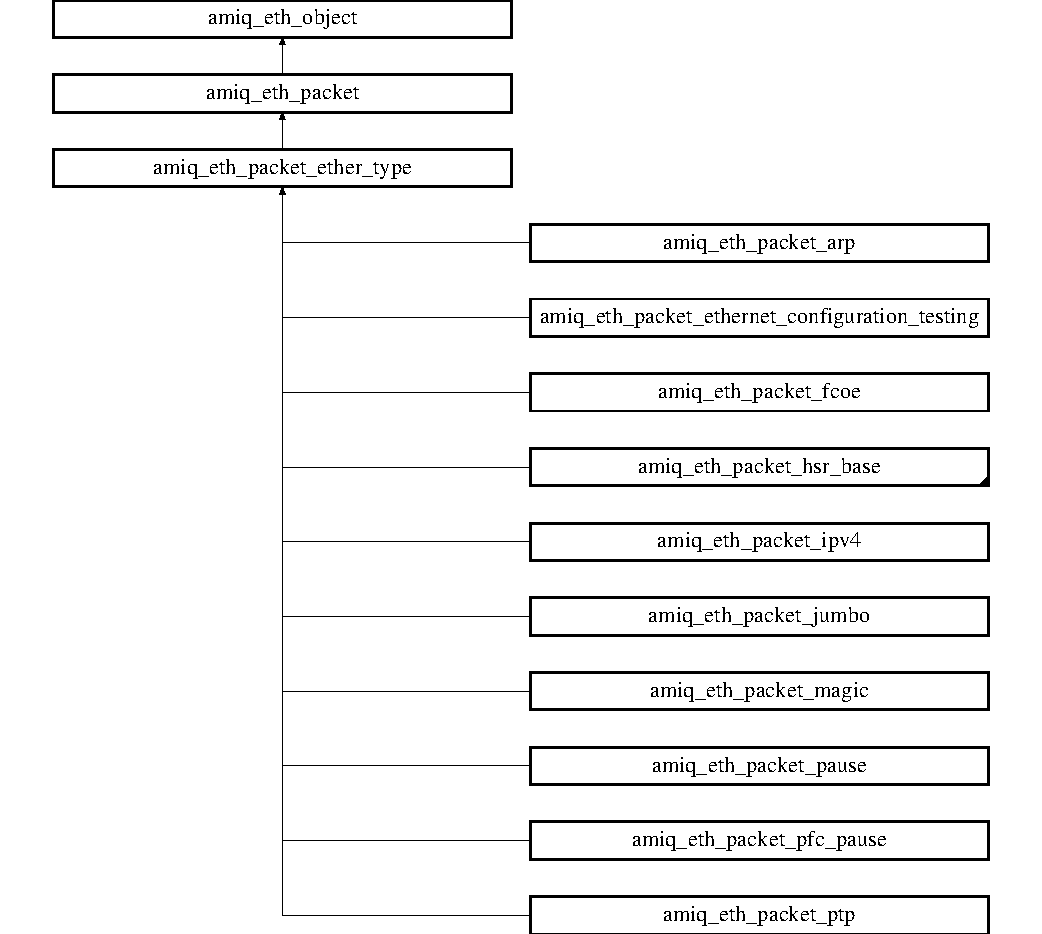
\includegraphics[height=12cm]{classamiq__eth__packet__ether__type}
\end{center}
\end{figure}
\subsection*{Public Member Functions}
\begin{DoxyCompactItemize}
\item 
\hyperlink{classamiq__eth__packet__ether__type_a1564c7b9fd6f3ecde8d224c2bb3f4294}{amiq\_\-eth\_\-packet\_\-ether\_\-type} ()
\item 
virtual \hyperlink{classamiq__eth__packet__ether__type_a7e5ab86fde67a32a33aa71871be5023b}{$\sim$amiq\_\-eth\_\-packet\_\-ether\_\-type} ()
\item 
virtual void \hyperlink{classamiq__eth__packet__ether__type_a9b2852fa1aaf278138fde2232e446f63}{do\_\-print} (ostream \&out) const 
\item 
virtual void \hyperlink{classamiq__eth__packet__ether__type_ac7056e1a4bc251384bcea25055ee62da}{pack\_\-ether\_\-type} (\hyperlink{classamiq__eth__packer}{amiq\_\-eth\_\-packer} \&packer) const 
\item 
virtual void \hyperlink{classamiq__eth__packet__ether__type_a62fe5f26a466f0bd0045599b89aa6926}{do\_\-pack} (\hyperlink{classamiq__eth__packer}{amiq\_\-eth\_\-packer} \&packer) const 
\item 
virtual void \hyperlink{classamiq__eth__packet__ether__type_a0c86ef80c46bbed384739b23e5efb0ef}{do\_\-unpack} (\hyperlink{classamiq__eth__packer}{amiq\_\-eth\_\-packer} \&packer)
\item 
virtual void \hyperlink{classamiq__eth__packet__ether__type_aaa85cf778650e1c1b377392a975cb7bc}{do\_\-pack\_\-for\_\-fcs} (\hyperlink{classamiq__eth__packer}{amiq\_\-eth\_\-packer} \&packer) const 
\end{DoxyCompactItemize}
\subsection*{Public Attributes}
\begin{DoxyCompactItemize}
\item 
\hyperlink{amiq__eth__types_8cpp_a37b16207afec6c164b234103e61309c4}{ethernet\_\-legal\_\-protocols} \hyperlink{classamiq__eth__packet__ether__type_a6d7d60a348004a078df2635936c8483a}{ether\_\-type}
\end{DoxyCompactItemize}


\subsection{Detailed Description}


Definition at line 32 of file amiq\_\-eth\_\-packet\_\-ether\_\-type.cpp.

\subsection{Constructor \& Destructor Documentation}
\hypertarget{classamiq__eth__packet__ether__type_a1564c7b9fd6f3ecde8d224c2bb3f4294}{
\index{amiq\_\-eth\_\-packet\_\-ether\_\-type@{amiq\_\-eth\_\-packet\_\-ether\_\-type}!amiq\_\-eth\_\-packet\_\-ether\_\-type@{amiq\_\-eth\_\-packet\_\-ether\_\-type}}
\index{amiq\_\-eth\_\-packet\_\-ether\_\-type@{amiq\_\-eth\_\-packet\_\-ether\_\-type}!amiq_eth_packet_ether_type@{amiq\_\-eth\_\-packet\_\-ether\_\-type}}
\subsubsection[{amiq\_\-eth\_\-packet\_\-ether\_\-type}]{\setlength{\rightskip}{0pt plus 5cm}amiq\_\-eth\_\-packet\_\-ether\_\-type::amiq\_\-eth\_\-packet\_\-ether\_\-type ()\hspace{0.3cm}{\ttfamily  \mbox{[}inline\mbox{]}}}}
\label{classamiq__eth__packet__ether__type_a1564c7b9fd6f3ecde8d224c2bb3f4294}


Definition at line 40 of file amiq\_\-eth\_\-packet\_\-ether\_\-type.cpp.

References ether\_\-type.\hypertarget{classamiq__eth__packet__ether__type_a7e5ab86fde67a32a33aa71871be5023b}{
\index{amiq\_\-eth\_\-packet\_\-ether\_\-type@{amiq\_\-eth\_\-packet\_\-ether\_\-type}!$\sim$amiq\_\-eth\_\-packet\_\-ether\_\-type@{$\sim$amiq\_\-eth\_\-packet\_\-ether\_\-type}}
\index{$\sim$amiq\_\-eth\_\-packet\_\-ether\_\-type@{$\sim$amiq\_\-eth\_\-packet\_\-ether\_\-type}!amiq_eth_packet_ether_type@{amiq\_\-eth\_\-packet\_\-ether\_\-type}}
\subsubsection[{$\sim$amiq\_\-eth\_\-packet\_\-ether\_\-type}]{\setlength{\rightskip}{0pt plus 5cm}virtual amiq\_\-eth\_\-packet\_\-ether\_\-type::$\sim$amiq\_\-eth\_\-packet\_\-ether\_\-type ()\hspace{0.3cm}{\ttfamily  \mbox{[}inline, virtual\mbox{]}}}}
\label{classamiq__eth__packet__ether__type_a7e5ab86fde67a32a33aa71871be5023b}


Definition at line 45 of file amiq\_\-eth\_\-packet\_\-ether\_\-type.cpp.

\subsection{Member Function Documentation}
\hypertarget{classamiq__eth__packet__ether__type_a62fe5f26a466f0bd0045599b89aa6926}{
\index{amiq\_\-eth\_\-packet\_\-ether\_\-type@{amiq\_\-eth\_\-packet\_\-ether\_\-type}!do\_\-pack@{do\_\-pack}}
\index{do\_\-pack@{do\_\-pack}!amiq_eth_packet_ether_type@{amiq\_\-eth\_\-packet\_\-ether\_\-type}}
\subsubsection[{do\_\-pack}]{\setlength{\rightskip}{0pt plus 5cm}virtual void amiq\_\-eth\_\-packet\_\-ether\_\-type::do\_\-pack ({\bf amiq\_\-eth\_\-packer} \& {\em packer}) const\hspace{0.3cm}{\ttfamily  \mbox{[}inline, virtual\mbox{]}}}}
\label{classamiq__eth__packet__ether__type_a62fe5f26a466f0bd0045599b89aa6926}


Reimplemented from \hyperlink{classamiq__eth__packet_ab580d89fb44208f5a0fe31443619473e}{amiq\_\-eth\_\-packet}.

Reimplemented in \hyperlink{classamiq__eth__packet__arp_aa0919231910bf804ffafd9b1b771785f}{amiq\_\-eth\_\-packet\_\-arp}, \hyperlink{classamiq__eth__packet__ethernet__configuration__testing_a4ae6c0485066d7661170544fa64c7e49}{amiq\_\-eth\_\-packet\_\-ethernet\_\-configuration\_\-testing}, \hyperlink{classamiq__eth__packet__fcoe_ae119ce0a219ea22eef14da61262afbb7}{amiq\_\-eth\_\-packet\_\-fcoe}, \hyperlink{classamiq__eth__packet__hsr__base_a6dc22f94409c889f248908b1454af8b0}{amiq\_\-eth\_\-packet\_\-hsr\_\-base}, \hyperlink{classamiq__eth__packet__hsr__standard_a1dce9b763e3222c2fe257b15df912514}{amiq\_\-eth\_\-packet\_\-hsr\_\-standard}, \hyperlink{classamiq__eth__packet__ipv4_a8130e24da66bbd16c4edc7b6a608a5e9}{amiq\_\-eth\_\-packet\_\-ipv4}, \hyperlink{classamiq__eth__packet__jumbo_a1f2906c7128a79c356e152368584d2e8}{amiq\_\-eth\_\-packet\_\-jumbo}, \hyperlink{classamiq__eth__packet__magic_ad026a187c1d882aa1698a3b0d4209472}{amiq\_\-eth\_\-packet\_\-magic}, \hyperlink{classamiq__eth__packet__pause_aaea61c8cafc5274eac5d2b5428876868}{amiq\_\-eth\_\-packet\_\-pause}, \hyperlink{classamiq__eth__packet__pfc__pause_ac06dfc3d16b73113bbd42460ddbc9c4b}{amiq\_\-eth\_\-packet\_\-pfc\_\-pause}, and \hyperlink{classamiq__eth__packet__ptp_a5d415af5fcb6ed2cb603aaf0105fdd43}{amiq\_\-eth\_\-packet\_\-ptp}.

Definition at line 67 of file amiq\_\-eth\_\-packet\_\-ether\_\-type.cpp.

References pack\_\-ether\_\-type().\hypertarget{classamiq__eth__packet__ether__type_aaa85cf778650e1c1b377392a975cb7bc}{
\index{amiq\_\-eth\_\-packet\_\-ether\_\-type@{amiq\_\-eth\_\-packet\_\-ether\_\-type}!do\_\-pack\_\-for\_\-fcs@{do\_\-pack\_\-for\_\-fcs}}
\index{do\_\-pack\_\-for\_\-fcs@{do\_\-pack\_\-for\_\-fcs}!amiq_eth_packet_ether_type@{amiq\_\-eth\_\-packet\_\-ether\_\-type}}
\subsubsection[{do\_\-pack\_\-for\_\-fcs}]{\setlength{\rightskip}{0pt plus 5cm}virtual void amiq\_\-eth\_\-packet\_\-ether\_\-type::do\_\-pack\_\-for\_\-fcs ({\bf amiq\_\-eth\_\-packer} \& {\em packer}) const\hspace{0.3cm}{\ttfamily  \mbox{[}inline, virtual\mbox{]}}}}
\label{classamiq__eth__packet__ether__type_aaa85cf778650e1c1b377392a975cb7bc}


Reimplemented from \hyperlink{classamiq__eth__packet_aacbc675df31e2674b5b4c73c9bd9961e}{amiq\_\-eth\_\-packet}.

Reimplemented in \hyperlink{classamiq__eth__packet__arp_aa94e012455f436aa874eb6e27e02b5fa}{amiq\_\-eth\_\-packet\_\-arp}, \hyperlink{classamiq__eth__packet__ipv4_a9292f2b244e6baae39ba4aeea7b97e8f}{amiq\_\-eth\_\-packet\_\-ipv4}, \hyperlink{classamiq__eth__packet__jumbo_ad1b7057e4292645ccb65b57bcea3a549}{amiq\_\-eth\_\-packet\_\-jumbo}, \hyperlink{classamiq__eth__packet__magic_a0a40225ac5c36e70f413cd6d8ffd9a24}{amiq\_\-eth\_\-packet\_\-magic}, and \hyperlink{classamiq__eth__packet__ptp_a68337ad7c7971f267b692dfbd92ede7b}{amiq\_\-eth\_\-packet\_\-ptp}.

Definition at line 84 of file amiq\_\-eth\_\-packet\_\-ether\_\-type.cpp.

References pack\_\-ether\_\-type().\hypertarget{classamiq__eth__packet__ether__type_a9b2852fa1aaf278138fde2232e446f63}{
\index{amiq\_\-eth\_\-packet\_\-ether\_\-type@{amiq\_\-eth\_\-packet\_\-ether\_\-type}!do\_\-print@{do\_\-print}}
\index{do\_\-print@{do\_\-print}!amiq_eth_packet_ether_type@{amiq\_\-eth\_\-packet\_\-ether\_\-type}}
\subsubsection[{do\_\-print}]{\setlength{\rightskip}{0pt plus 5cm}virtual void amiq\_\-eth\_\-packet\_\-ether\_\-type::do\_\-print (ostream \& {\em out}) const\hspace{0.3cm}{\ttfamily  \mbox{[}inline, virtual\mbox{]}}}}
\label{classamiq__eth__packet__ether__type_a9b2852fa1aaf278138fde2232e446f63}


Reimplemented from \hyperlink{classamiq__eth__packet_aa179c700ae183f1b884a9222a73fed4e}{amiq\_\-eth\_\-packet}.

Reimplemented in \hyperlink{classamiq__eth__packet__arp_abbb862d7b7abe9b1c6d49455f80f6921}{amiq\_\-eth\_\-packet\_\-arp}, \hyperlink{classamiq__eth__packet__ethernet__configuration__testing_aaac4abb2c0104900e30360871e01bbbd}{amiq\_\-eth\_\-packet\_\-ethernet\_\-configuration\_\-testing}, \hyperlink{classamiq__eth__packet__fcoe_a39fa215f83aa71ff06c5fd699de8e427}{amiq\_\-eth\_\-packet\_\-fcoe}, \hyperlink{classamiq__eth__packet__hsr__base_a83b7ccb4b601e00ba5cfbbfde6658632}{amiq\_\-eth\_\-packet\_\-hsr\_\-base}, \hyperlink{classamiq__eth__packet__hsr__standard_abaa39d881f90e05ae4acbb7fe5ebca0d}{amiq\_\-eth\_\-packet\_\-hsr\_\-standard}, \hyperlink{classamiq__eth__packet__ipv4_a5e93e2455918061cdc524f30626d4043}{amiq\_\-eth\_\-packet\_\-ipv4}, \hyperlink{classamiq__eth__packet__jumbo_a744d47397c29884a7da15e5582b331a2}{amiq\_\-eth\_\-packet\_\-jumbo}, \hyperlink{classamiq__eth__packet__magic_a57354d611adb80b1a8f4ad00c4f307a3}{amiq\_\-eth\_\-packet\_\-magic}, \hyperlink{classamiq__eth__packet__pause_a7ea960bd9c079375b0d4cd72a762d695}{amiq\_\-eth\_\-packet\_\-pause}, \hyperlink{classamiq__eth__packet__pfc__pause_a58c67ea445a72bc6c1c584625d642899}{amiq\_\-eth\_\-packet\_\-pfc\_\-pause}, and \hyperlink{classamiq__eth__packet__ptp_a52db9ab62ab743317a7ca4745a823a82}{amiq\_\-eth\_\-packet\_\-ptp}.

Definition at line 51 of file amiq\_\-eth\_\-packet\_\-ether\_\-type.cpp.

References AMIQ\_\-ETH\_\-FIELD\_\-SEPARATOR, and ether\_\-type.\hypertarget{classamiq__eth__packet__ether__type_a0c86ef80c46bbed384739b23e5efb0ef}{
\index{amiq\_\-eth\_\-packet\_\-ether\_\-type@{amiq\_\-eth\_\-packet\_\-ether\_\-type}!do\_\-unpack@{do\_\-unpack}}
\index{do\_\-unpack@{do\_\-unpack}!amiq_eth_packet_ether_type@{amiq\_\-eth\_\-packet\_\-ether\_\-type}}
\subsubsection[{do\_\-unpack}]{\setlength{\rightskip}{0pt plus 5cm}virtual void amiq\_\-eth\_\-packet\_\-ether\_\-type::do\_\-unpack ({\bf amiq\_\-eth\_\-packer} \& {\em packer})\hspace{0.3cm}{\ttfamily  \mbox{[}inline, virtual\mbox{]}}}}
\label{classamiq__eth__packet__ether__type_a0c86ef80c46bbed384739b23e5efb0ef}


Reimplemented from \hyperlink{classamiq__eth__packet_a909eb3860185125564fa530496ed1c9e}{amiq\_\-eth\_\-packet}.

Reimplemented in \hyperlink{classamiq__eth__packet__arp_afa8463360e8e62b24e1171093b00a798}{amiq\_\-eth\_\-packet\_\-arp}, \hyperlink{classamiq__eth__packet__ethernet__configuration__testing_aff2640ccc3b20b80b16bb6ab20842f76}{amiq\_\-eth\_\-packet\_\-ethernet\_\-configuration\_\-testing}, \hyperlink{classamiq__eth__packet__fcoe_afb550561999badc5693283b852be2f70}{amiq\_\-eth\_\-packet\_\-fcoe}, \hyperlink{classamiq__eth__packet__hsr__base_ae61de71bd90f7a1c605e094845af5ccc}{amiq\_\-eth\_\-packet\_\-hsr\_\-base}, \hyperlink{classamiq__eth__packet__hsr__standard_aac95578ea89db3bd0ec190ca87e731c8}{amiq\_\-eth\_\-packet\_\-hsr\_\-standard}, \hyperlink{classamiq__eth__packet__ipv4_af85e08566b37953edee4566c40400f05}{amiq\_\-eth\_\-packet\_\-ipv4}, \hyperlink{classamiq__eth__packet__jumbo_a2d1f1c25847363d774336f8828384635}{amiq\_\-eth\_\-packet\_\-jumbo}, \hyperlink{classamiq__eth__packet__magic_a400a90ae523af44eb0c38ba64ea6afe7}{amiq\_\-eth\_\-packet\_\-magic}, \hyperlink{classamiq__eth__packet__pause_aa458964a73aa61bca99cb30ffa56f54c}{amiq\_\-eth\_\-packet\_\-pause}, \hyperlink{classamiq__eth__packet__pfc__pause_abc86009030a38ab03469c697ffec73f6}{amiq\_\-eth\_\-packet\_\-pfc\_\-pause}, and \hyperlink{classamiq__eth__packet__ptp_a831addd66dff7e42f2e2e9edb6f976b3}{amiq\_\-eth\_\-packet\_\-ptp}.

Definition at line 74 of file amiq\_\-eth\_\-packet\_\-ether\_\-type.cpp.

References amiq\_\-eth\_\-do\_\-unpack(), and ether\_\-type.\hypertarget{classamiq__eth__packet__ether__type_ac7056e1a4bc251384bcea25055ee62da}{
\index{amiq\_\-eth\_\-packet\_\-ether\_\-type@{amiq\_\-eth\_\-packet\_\-ether\_\-type}!pack\_\-ether\_\-type@{pack\_\-ether\_\-type}}
\index{pack\_\-ether\_\-type@{pack\_\-ether\_\-type}!amiq_eth_packet_ether_type@{amiq\_\-eth\_\-packet\_\-ether\_\-type}}
\subsubsection[{pack\_\-ether\_\-type}]{\setlength{\rightskip}{0pt plus 5cm}virtual void amiq\_\-eth\_\-packet\_\-ether\_\-type::pack\_\-ether\_\-type ({\bf amiq\_\-eth\_\-packer} \& {\em packer}) const\hspace{0.3cm}{\ttfamily  \mbox{[}inline, virtual\mbox{]}}}}
\label{classamiq__eth__packet__ether__type_ac7056e1a4bc251384bcea25055ee62da}


Definition at line 60 of file amiq\_\-eth\_\-packet\_\-ether\_\-type.cpp.

References amiq\_\-eth\_\-do\_\-pack(), and ether\_\-type.

Referenced by do\_\-pack(), and do\_\-pack\_\-for\_\-fcs().

\subsection{Member Data Documentation}
\hypertarget{classamiq__eth__packet__ether__type_a6d7d60a348004a078df2635936c8483a}{
\index{amiq\_\-eth\_\-packet\_\-ether\_\-type@{amiq\_\-eth\_\-packet\_\-ether\_\-type}!ether\_\-type@{ether\_\-type}}
\index{ether\_\-type@{ether\_\-type}!amiq_eth_packet_ether_type@{amiq\_\-eth\_\-packet\_\-ether\_\-type}}
\subsubsection[{ether\_\-type}]{\setlength{\rightskip}{0pt plus 5cm}{\bf ethernet\_\-legal\_\-protocols} {\bf amiq\_\-eth\_\-packet\_\-ether\_\-type::ether\_\-type}}}
\label{classamiq__eth__packet__ether__type_a6d7d60a348004a078df2635936c8483a}


Definition at line 37 of file amiq\_\-eth\_\-packet\_\-ether\_\-type.cpp.

Referenced by amiq\_\-eth\_\-packet\_\-ether\_\-type(), amiq\_\-eth\_\-packet\_\-ethernet\_\-configuration\_\-testing::amiq\_\-eth\_\-packet\_\-ethernet\_\-configuration\_\-testing(), amiq\_\-eth\_\-packet\_\-fcoe::amiq\_\-eth\_\-packet\_\-fcoe(), amiq\_\-eth\_\-packet\_\-hsr\_\-base::amiq\_\-eth\_\-packet\_\-hsr\_\-base(), amiq\_\-eth\_\-packet\_\-pause::amiq\_\-eth\_\-packet\_\-pause(), amiq\_\-eth\_\-packet\_\-pfc\_\-pause::amiq\_\-eth\_\-packet\_\-pfc\_\-pause(), amiq\_\-eth\_\-packet\_\-ptp::amiq\_\-eth\_\-packet\_\-ptp(), do\_\-print(), do\_\-unpack(), and pack\_\-ether\_\-type().

The documentation for this class was generated from the following file:\begin{DoxyCompactItemize}
\item 
/home/cristian.slav/work/amiq/projects/sv/amiq\_\-eth/sc/\hyperlink{amiq__eth__packet__ether__type_8cpp}{amiq\_\-eth\_\-packet\_\-ether\_\-type.cpp}\end{DoxyCompactItemize}

\hypertarget{classamiq__eth__packet__ethernet__configuration__testing}{
\section{amiq\_\-eth\_\-packet\_\-ethernet\_\-configuration\_\-testing Class Reference}
\label{classamiq__eth__packet__ethernet__configuration__testing}\index{amiq\_\-eth\_\-packet\_\-ethernet\_\-configuration\_\-testing@{amiq\_\-eth\_\-packet\_\-ethernet\_\-configuration\_\-testing}}
}
Inheritance diagram for amiq\_\-eth\_\-packet\_\-ethernet\_\-configuration\_\-testing::\begin{figure}[H]
\begin{center}
\leavevmode
\includegraphics[height=4cm]{classamiq__eth__packet__ethernet__configuration__testing}
\end{center}
\end{figure}
\subsection*{Public Member Functions}
\begin{DoxyCompactItemize}
\item 
\hyperlink{classamiq__eth__packet__ethernet__configuration__testing_aa8c3ffe26aecf8f091bef33b574cfefc}{amiq\_\-eth\_\-packet\_\-ethernet\_\-configuration\_\-testing} ()
\item 
virtual \hyperlink{classamiq__eth__packet__ethernet__configuration__testing_a7841ec746b28b5480d500606aeeac506}{$\sim$amiq\_\-eth\_\-packet\_\-ethernet\_\-configuration\_\-testing} ()
\item 
virtual void \hyperlink{classamiq__eth__packet__ethernet__configuration__testing_aaac4abb2c0104900e30360871e01bbbd}{do\_\-print} (ostream \&out) const 
\item 
virtual void \hyperlink{classamiq__eth__packet__ethernet__configuration__testing_a4ae6c0485066d7661170544fa64c7e49}{do\_\-pack} (\hyperlink{classamiq__eth__packer}{amiq\_\-eth\_\-packer} \&packer) const 
\item 
virtual void \hyperlink{classamiq__eth__packet__ethernet__configuration__testing_aff2640ccc3b20b80b16bb6ab20842f76}{do\_\-unpack} (\hyperlink{classamiq__eth__packer}{amiq\_\-eth\_\-packer} \&packer)
\item 
virtual tlm\_\-generic\_\-payload $\ast$ \hyperlink{classamiq__eth__packet__ethernet__configuration__testing_a0134f20913a67a5dafe334a450be8bb3}{to\_\-generic\_\-payload} () const 
\end{DoxyCompactItemize}
\subsection*{Public Attributes}
\begin{DoxyCompactItemize}
\item 
\hyperlink{amiq__eth__types_8cpp_aaeb6b67f18d2fb2fcd870c5db61c5a9e}{amiq\_\-eth\_\-ethernet\_\-configuration\_\-testing\_\-skipcount} \hyperlink{classamiq__eth__packet__ethernet__configuration__testing_a0e0c3dab008be4317aa19dfbe1a75be1}{skipcount}
\item 
\hyperlink{amiq__eth__types_8cpp_a11e211f9a3ab99b4cf88c206bd785658}{amiq\_\-eth\_\-ethernet\_\-configuration\_\-testing\_\-function} \hyperlink{classamiq__eth__packet__ethernet__configuration__testing_a8f0790eac9bf1d803112ce23788e4fc7}{cfg\_\-test\_\-function}
\item 
\hyperlink{amiq__eth__types_8cpp_a1381089182c9f964cb292e74680df434}{amiq\_\-eth\_\-ethernet\_\-configuration\_\-testing\_\-data\_\-size} \hyperlink{classamiq__eth__packet__ethernet__configuration__testing_a296a5b8f577059bed0991b13b4337c83}{data\_\-size}
\item 
\hyperlink{amiq__eth__types_8cpp_a3595a0a508d433d383d3e5521fc0b723}{amiq\_\-eth\_\-data} $\ast$ \hyperlink{classamiq__eth__packet__ethernet__configuration__testing_a93c7b061e19eafe5aa00fdf822e26008}{data}
\item 
\hyperlink{amiq__eth__types_8cpp_adb511dc715b55539c6abdad1de981a9f}{amiq\_\-eth\_\-fcs} \hyperlink{classamiq__eth__packet__ethernet__configuration__testing_a5e8b2f14ebe61f3e98618033ebe246e4}{fcs}
\item 
bool \hyperlink{classamiq__eth__packet__ethernet__configuration__testing_a9804a9d571b8172916ee9dd61d1860c5}{print\_\-lists}
\end{DoxyCompactItemize}


\subsection{Detailed Description}


Definition at line 28 of file amiq\_\-eth\_\-packet\_\-ethernet\_\-configuration\_\-testing.cpp.

\subsection{Constructor \& Destructor Documentation}
\hypertarget{classamiq__eth__packet__ethernet__configuration__testing_aa8c3ffe26aecf8f091bef33b574cfefc}{
\index{amiq\_\-eth\_\-packet\_\-ethernet\_\-configuration\_\-testing@{amiq\_\-eth\_\-packet\_\-ethernet\_\-configuration\_\-testing}!amiq\_\-eth\_\-packet\_\-ethernet\_\-configuration\_\-testing@{amiq\_\-eth\_\-packet\_\-ethernet\_\-configuration\_\-testing}}
\index{amiq\_\-eth\_\-packet\_\-ethernet\_\-configuration\_\-testing@{amiq\_\-eth\_\-packet\_\-ethernet\_\-configuration\_\-testing}!amiq_eth_packet_ethernet_configuration_testing@{amiq\_\-eth\_\-packet\_\-ethernet\_\-configuration\_\-testing}}
\subsubsection[{amiq\_\-eth\_\-packet\_\-ethernet\_\-configuration\_\-testing}]{\setlength{\rightskip}{0pt plus 5cm}amiq\_\-eth\_\-packet\_\-ethernet\_\-configuration\_\-testing::amiq\_\-eth\_\-packet\_\-ethernet\_\-configuration\_\-testing ()\hspace{0.3cm}{\ttfamily  \mbox{[}inline\mbox{]}}}}
\label{classamiq__eth__packet__ethernet__configuration__testing_aa8c3ffe26aecf8f091bef33b574cfefc}


Definition at line 46 of file amiq\_\-eth\_\-packet\_\-ethernet\_\-configuration\_\-testing.cpp.

References amiq\_\-eth\_\-packet\_\-ether\_\-type::ether\_\-type, print\_\-lists, and SC\_\-AMIQ\_\-ETH\_\-ETHERNET\_\-CONFIGURATION\_\-TESTING\_\-PROTOCOL.\hypertarget{classamiq__eth__packet__ethernet__configuration__testing_a7841ec746b28b5480d500606aeeac506}{
\index{amiq\_\-eth\_\-packet\_\-ethernet\_\-configuration\_\-testing@{amiq\_\-eth\_\-packet\_\-ethernet\_\-configuration\_\-testing}!$\sim$amiq\_\-eth\_\-packet\_\-ethernet\_\-configuration\_\-testing@{$\sim$amiq\_\-eth\_\-packet\_\-ethernet\_\-configuration\_\-testing}}
\index{$\sim$amiq\_\-eth\_\-packet\_\-ethernet\_\-configuration\_\-testing@{$\sim$amiq\_\-eth\_\-packet\_\-ethernet\_\-configuration\_\-testing}!amiq_eth_packet_ethernet_configuration_testing@{amiq\_\-eth\_\-packet\_\-ethernet\_\-configuration\_\-testing}}
\subsubsection[{$\sim$amiq\_\-eth\_\-packet\_\-ethernet\_\-configuration\_\-testing}]{\setlength{\rightskip}{0pt plus 5cm}virtual amiq\_\-eth\_\-packet\_\-ethernet\_\-configuration\_\-testing::$\sim$amiq\_\-eth\_\-packet\_\-ethernet\_\-configuration\_\-testing ()\hspace{0.3cm}{\ttfamily  \mbox{[}inline, virtual\mbox{]}}}}
\label{classamiq__eth__packet__ethernet__configuration__testing_a7841ec746b28b5480d500606aeeac506}


Definition at line 52 of file amiq\_\-eth\_\-packet\_\-ethernet\_\-configuration\_\-testing.cpp.

\subsection{Member Function Documentation}
\hypertarget{classamiq__eth__packet__ethernet__configuration__testing_a4ae6c0485066d7661170544fa64c7e49}{
\index{amiq\_\-eth\_\-packet\_\-ethernet\_\-configuration\_\-testing@{amiq\_\-eth\_\-packet\_\-ethernet\_\-configuration\_\-testing}!do\_\-pack@{do\_\-pack}}
\index{do\_\-pack@{do\_\-pack}!amiq_eth_packet_ethernet_configuration_testing@{amiq\_\-eth\_\-packet\_\-ethernet\_\-configuration\_\-testing}}
\subsubsection[{do\_\-pack}]{\setlength{\rightskip}{0pt plus 5cm}virtual void amiq\_\-eth\_\-packet\_\-ethernet\_\-configuration\_\-testing::do\_\-pack ({\bf amiq\_\-eth\_\-packer} \& {\em packer}) const\hspace{0.3cm}{\ttfamily  \mbox{[}inline, virtual\mbox{]}}}}
\label{classamiq__eth__packet__ethernet__configuration__testing_a4ae6c0485066d7661170544fa64c7e49}


Reimplemented from \hyperlink{classamiq__eth__packet__ether__type_a62fe5f26a466f0bd0045599b89aa6926}{amiq\_\-eth\_\-packet\_\-ether\_\-type}.

Definition at line 73 of file amiq\_\-eth\_\-packet\_\-ethernet\_\-configuration\_\-testing.cpp.

References amiq\_\-eth\_\-do\_\-pack(), cfg\_\-test\_\-function, data, data\_\-size, fcs, and skipcount.\hypertarget{classamiq__eth__packet__ethernet__configuration__testing_aaac4abb2c0104900e30360871e01bbbd}{
\index{amiq\_\-eth\_\-packet\_\-ethernet\_\-configuration\_\-testing@{amiq\_\-eth\_\-packet\_\-ethernet\_\-configuration\_\-testing}!do\_\-print@{do\_\-print}}
\index{do\_\-print@{do\_\-print}!amiq_eth_packet_ethernet_configuration_testing@{amiq\_\-eth\_\-packet\_\-ethernet\_\-configuration\_\-testing}}
\subsubsection[{do\_\-print}]{\setlength{\rightskip}{0pt plus 5cm}virtual void amiq\_\-eth\_\-packet\_\-ethernet\_\-configuration\_\-testing::do\_\-print (ostream \& {\em out}) const\hspace{0.3cm}{\ttfamily  \mbox{[}inline, virtual\mbox{]}}}}
\label{classamiq__eth__packet__ethernet__configuration__testing_aaac4abb2c0104900e30360871e01bbbd}


Reimplemented from \hyperlink{classamiq__eth__packet__ether__type_a9b2852fa1aaf278138fde2232e446f63}{amiq\_\-eth\_\-packet\_\-ether\_\-type}.

Definition at line 57 of file amiq\_\-eth\_\-packet\_\-ethernet\_\-configuration\_\-testing.cpp.

References AMIQ\_\-ETH\_\-FIELD\_\-SEPARATOR, cfg\_\-test\_\-function, data, data\_\-size, fcs, print\_\-lists, and skipcount.\hypertarget{classamiq__eth__packet__ethernet__configuration__testing_aff2640ccc3b20b80b16bb6ab20842f76}{
\index{amiq\_\-eth\_\-packet\_\-ethernet\_\-configuration\_\-testing@{amiq\_\-eth\_\-packet\_\-ethernet\_\-configuration\_\-testing}!do\_\-unpack@{do\_\-unpack}}
\index{do\_\-unpack@{do\_\-unpack}!amiq_eth_packet_ethernet_configuration_testing@{amiq\_\-eth\_\-packet\_\-ethernet\_\-configuration\_\-testing}}
\subsubsection[{do\_\-unpack}]{\setlength{\rightskip}{0pt plus 5cm}virtual void amiq\_\-eth\_\-packet\_\-ethernet\_\-configuration\_\-testing::do\_\-unpack ({\bf amiq\_\-eth\_\-packer} \& {\em packer})\hspace{0.3cm}{\ttfamily  \mbox{[}inline, virtual\mbox{]}}}}
\label{classamiq__eth__packet__ethernet__configuration__testing_aff2640ccc3b20b80b16bb6ab20842f76}


Reimplemented from \hyperlink{classamiq__eth__packet__ether__type_a0c86ef80c46bbed384739b23e5efb0ef}{amiq\_\-eth\_\-packet\_\-ether\_\-type}.

Definition at line 94 of file amiq\_\-eth\_\-packet\_\-ethernet\_\-configuration\_\-testing.cpp.

References amiq\_\-eth\_\-do\_\-unpack(), cfg\_\-test\_\-function, data, data\_\-size, fcs, and skipcount.\hypertarget{classamiq__eth__packet__ethernet__configuration__testing_a0134f20913a67a5dafe334a450be8bb3}{
\index{amiq\_\-eth\_\-packet\_\-ethernet\_\-configuration\_\-testing@{amiq\_\-eth\_\-packet\_\-ethernet\_\-configuration\_\-testing}!to\_\-generic\_\-payload@{to\_\-generic\_\-payload}}
\index{to\_\-generic\_\-payload@{to\_\-generic\_\-payload}!amiq_eth_packet_ethernet_configuration_testing@{amiq\_\-eth\_\-packet\_\-ethernet\_\-configuration\_\-testing}}
\subsubsection[{to\_\-generic\_\-payload}]{\setlength{\rightskip}{0pt plus 5cm}virtual tlm\_\-generic\_\-payload$\ast$ amiq\_\-eth\_\-packet\_\-ethernet\_\-configuration\_\-testing::to\_\-generic\_\-payload () const\hspace{0.3cm}{\ttfamily  \mbox{[}inline, virtual\mbox{]}}}}
\label{classamiq__eth__packet__ethernet__configuration__testing_a0134f20913a67a5dafe334a450be8bb3}


Reimplemented from \hyperlink{classamiq__eth__packet_a6dd92751d8172eeaa347d71bb415b0d5}{amiq\_\-eth\_\-packet}.

Definition at line 117 of file amiq\_\-eth\_\-packet\_\-ethernet\_\-configuration\_\-testing.cpp.

References AMIQ\_\-ETH\_\-PACKET\_\-ETHERNET\_\-CONFIGURATION\_\-TESTING\_\-CODE.

\subsection{Member Data Documentation}
\hypertarget{classamiq__eth__packet__ethernet__configuration__testing_a8f0790eac9bf1d803112ce23788e4fc7}{
\index{amiq\_\-eth\_\-packet\_\-ethernet\_\-configuration\_\-testing@{amiq\_\-eth\_\-packet\_\-ethernet\_\-configuration\_\-testing}!cfg\_\-test\_\-function@{cfg\_\-test\_\-function}}
\index{cfg\_\-test\_\-function@{cfg\_\-test\_\-function}!amiq_eth_packet_ethernet_configuration_testing@{amiq\_\-eth\_\-packet\_\-ethernet\_\-configuration\_\-testing}}
\subsubsection[{cfg\_\-test\_\-function}]{\setlength{\rightskip}{0pt plus 5cm}{\bf amiq\_\-eth\_\-ethernet\_\-configuration\_\-testing\_\-function} {\bf amiq\_\-eth\_\-packet\_\-ethernet\_\-configuration\_\-testing::cfg\_\-test\_\-function}}}
\label{classamiq__eth__packet__ethernet__configuration__testing_a8f0790eac9bf1d803112ce23788e4fc7}


Definition at line 35 of file amiq\_\-eth\_\-packet\_\-ethernet\_\-configuration\_\-testing.cpp.

Referenced by do\_\-pack(), do\_\-print(), and do\_\-unpack().\hypertarget{classamiq__eth__packet__ethernet__configuration__testing_a93c7b061e19eafe5aa00fdf822e26008}{
\index{amiq\_\-eth\_\-packet\_\-ethernet\_\-configuration\_\-testing@{amiq\_\-eth\_\-packet\_\-ethernet\_\-configuration\_\-testing}!data@{data}}
\index{data@{data}!amiq_eth_packet_ethernet_configuration_testing@{amiq\_\-eth\_\-packet\_\-ethernet\_\-configuration\_\-testing}}
\subsubsection[{data}]{\setlength{\rightskip}{0pt plus 5cm}{\bf amiq\_\-eth\_\-data}$\ast$ {\bf amiq\_\-eth\_\-packet\_\-ethernet\_\-configuration\_\-testing::data}}}
\label{classamiq__eth__packet__ethernet__configuration__testing_a93c7b061e19eafe5aa00fdf822e26008}


Definition at line 38 of file amiq\_\-eth\_\-packet\_\-ethernet\_\-configuration\_\-testing.cpp.

Referenced by do\_\-pack(), do\_\-print(), and do\_\-unpack().\hypertarget{classamiq__eth__packet__ethernet__configuration__testing_a296a5b8f577059bed0991b13b4337c83}{
\index{amiq\_\-eth\_\-packet\_\-ethernet\_\-configuration\_\-testing@{amiq\_\-eth\_\-packet\_\-ethernet\_\-configuration\_\-testing}!data\_\-size@{data\_\-size}}
\index{data\_\-size@{data\_\-size}!amiq_eth_packet_ethernet_configuration_testing@{amiq\_\-eth\_\-packet\_\-ethernet\_\-configuration\_\-testing}}
\subsubsection[{data\_\-size}]{\setlength{\rightskip}{0pt plus 5cm}{\bf amiq\_\-eth\_\-ethernet\_\-configuration\_\-testing\_\-data\_\-size} {\bf amiq\_\-eth\_\-packet\_\-ethernet\_\-configuration\_\-testing::data\_\-size}}}
\label{classamiq__eth__packet__ethernet__configuration__testing_a296a5b8f577059bed0991b13b4337c83}


Definition at line 37 of file amiq\_\-eth\_\-packet\_\-ethernet\_\-configuration\_\-testing.cpp.

Referenced by do\_\-pack(), do\_\-print(), and do\_\-unpack().\hypertarget{classamiq__eth__packet__ethernet__configuration__testing_a5e8b2f14ebe61f3e98618033ebe246e4}{
\index{amiq\_\-eth\_\-packet\_\-ethernet\_\-configuration\_\-testing@{amiq\_\-eth\_\-packet\_\-ethernet\_\-configuration\_\-testing}!fcs@{fcs}}
\index{fcs@{fcs}!amiq_eth_packet_ethernet_configuration_testing@{amiq\_\-eth\_\-packet\_\-ethernet\_\-configuration\_\-testing}}
\subsubsection[{fcs}]{\setlength{\rightskip}{0pt plus 5cm}{\bf amiq\_\-eth\_\-fcs} {\bf amiq\_\-eth\_\-packet\_\-ethernet\_\-configuration\_\-testing::fcs}}}
\label{classamiq__eth__packet__ethernet__configuration__testing_a5e8b2f14ebe61f3e98618033ebe246e4}


Definition at line 40 of file amiq\_\-eth\_\-packet\_\-ethernet\_\-configuration\_\-testing.cpp.

Referenced by do\_\-pack(), do\_\-print(), and do\_\-unpack().\hypertarget{classamiq__eth__packet__ethernet__configuration__testing_a9804a9d571b8172916ee9dd61d1860c5}{
\index{amiq\_\-eth\_\-packet\_\-ethernet\_\-configuration\_\-testing@{amiq\_\-eth\_\-packet\_\-ethernet\_\-configuration\_\-testing}!print\_\-lists@{print\_\-lists}}
\index{print\_\-lists@{print\_\-lists}!amiq_eth_packet_ethernet_configuration_testing@{amiq\_\-eth\_\-packet\_\-ethernet\_\-configuration\_\-testing}}
\subsubsection[{print\_\-lists}]{\setlength{\rightskip}{0pt plus 5cm}bool {\bf amiq\_\-eth\_\-packet\_\-ethernet\_\-configuration\_\-testing::print\_\-lists}}}
\label{classamiq__eth__packet__ethernet__configuration__testing_a9804a9d571b8172916ee9dd61d1860c5}


Definition at line 43 of file amiq\_\-eth\_\-packet\_\-ethernet\_\-configuration\_\-testing.cpp.

Referenced by amiq\_\-eth\_\-packet\_\-ethernet\_\-configuration\_\-testing(), and do\_\-print().\hypertarget{classamiq__eth__packet__ethernet__configuration__testing_a0e0c3dab008be4317aa19dfbe1a75be1}{
\index{amiq\_\-eth\_\-packet\_\-ethernet\_\-configuration\_\-testing@{amiq\_\-eth\_\-packet\_\-ethernet\_\-configuration\_\-testing}!skipcount@{skipcount}}
\index{skipcount@{skipcount}!amiq_eth_packet_ethernet_configuration_testing@{amiq\_\-eth\_\-packet\_\-ethernet\_\-configuration\_\-testing}}
\subsubsection[{skipcount}]{\setlength{\rightskip}{0pt plus 5cm}{\bf amiq\_\-eth\_\-ethernet\_\-configuration\_\-testing\_\-skipcount} {\bf amiq\_\-eth\_\-packet\_\-ethernet\_\-configuration\_\-testing::skipcount}}}
\label{classamiq__eth__packet__ethernet__configuration__testing_a0e0c3dab008be4317aa19dfbe1a75be1}


Definition at line 33 of file amiq\_\-eth\_\-packet\_\-ethernet\_\-configuration\_\-testing.cpp.

Referenced by do\_\-pack(), do\_\-print(), and do\_\-unpack().

The documentation for this class was generated from the following file:\begin{DoxyCompactItemize}
\item 
/home/cristian.slav/work/amiq/projects/sv/amiq\_\-eth/sc/\hyperlink{amiq__eth__packet__ethernet__configuration__testing_8cpp}{amiq\_\-eth\_\-packet\_\-ethernet\_\-configuration\_\-testing.cpp}\end{DoxyCompactItemize}

\hypertarget{classamiq__eth__packet__fcoe}{
\section{amiq\_\-eth\_\-packet\_\-fcoe Class Reference}
\label{classamiq__eth__packet__fcoe}\index{amiq\_\-eth\_\-packet\_\-fcoe@{amiq\_\-eth\_\-packet\_\-fcoe}}
}
Inheritance diagram for amiq\_\-eth\_\-packet\_\-fcoe::\begin{figure}[H]
\begin{center}
\leavevmode
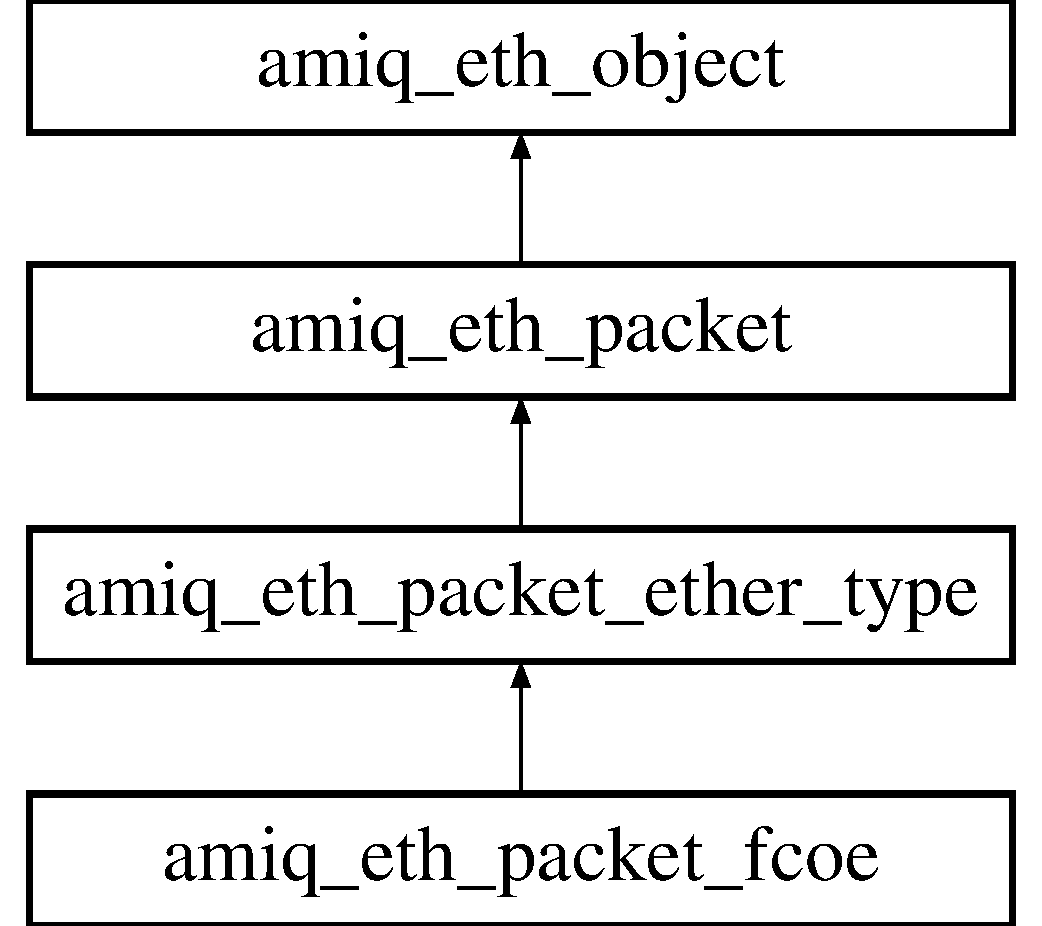
\includegraphics[height=4cm]{classamiq__eth__packet__fcoe}
\end{center}
\end{figure}
\subsection*{Public Member Functions}
\begin{DoxyCompactItemize}
\item 
\hyperlink{classamiq__eth__packet__fcoe_a8f9a82423c47abe1533b65751bc75e19}{amiq\_\-eth\_\-packet\_\-fcoe} ()
\item 
virtual \hyperlink{classamiq__eth__packet__fcoe_a44032a18eefcad771294b141167dcf14}{$\sim$amiq\_\-eth\_\-packet\_\-fcoe} ()
\item 
virtual void \hyperlink{classamiq__eth__packet__fcoe_a39fa215f83aa71ff06c5fd699de8e427}{do\_\-print} (ostream \&out) const 
\item 
virtual void \hyperlink{classamiq__eth__packet__fcoe_ae119ce0a219ea22eef14da61262afbb7}{do\_\-pack} (\hyperlink{classamiq__eth__packer}{amiq\_\-eth\_\-packer} \&packer) const 
\item 
virtual void \hyperlink{classamiq__eth__packet__fcoe_afb550561999badc5693283b852be2f70}{do\_\-unpack} (\hyperlink{classamiq__eth__packer}{amiq\_\-eth\_\-packer} \&packer)
\item 
virtual tlm\_\-generic\_\-payload $\ast$ \hyperlink{classamiq__eth__packet__fcoe_aa341b2f7df8abf278713e98015565c9f}{to\_\-generic\_\-payload} () const 
\end{DoxyCompactItemize}
\subsection*{Public Attributes}
\begin{DoxyCompactItemize}
\item 
\hyperlink{amiq__eth__types_8cpp_a52c27a397c2f1734227ff0fa20c3c463}{amiq\_\-eth\_\-fcoe\_\-version} \hyperlink{classamiq__eth__packet__fcoe_ad8ebe22dab7fcf728dbcb1353aead75a}{version}
\item 
\hyperlink{amiq__eth__types_8cpp_ab91426b193c9d785b26eab0fafeb37d4}{amiq\_\-eth\_\-fcoe\_\-reserved\_\-size} $\ast$ \hyperlink{classamiq__eth__packet__fcoe_a12c47cb7c8c88a33452e77cc939a537e}{fcoe\_\-reserved\_\-before\_\-sof}
\item 
\hyperlink{amiq__eth__types_8cpp_af76674e5304b9edc017f724a00bb450c}{amiq\_\-sof\_\-legal} \hyperlink{classamiq__eth__packet__fcoe_aa6a32da303dff37582cf2aa1ec127531}{sof}
\item 
\hyperlink{amiq__eth__types_8cpp_a6c8c792413bc1b4fdfcef78d585dc59b}{amiq\_\-eth\_\-fcoe\_\-frame\_\-size} \hyperlink{classamiq__eth__packet__fcoe_a3bff6efa35437af20ee1bc17af91ec45}{fc\_\-frame\_\-size}
\item 
\hyperlink{amiq__eth__types_8cpp_a3595a0a508d433d383d3e5521fc0b723}{amiq\_\-eth\_\-data} $\ast$ \hyperlink{classamiq__eth__packet__fcoe_a64d80e48f4ede107bb86908f9f1b8b1b}{fc\_\-frame}
\item 
\hyperlink{amiq__eth__types_8cpp_af8426b958ea3d0f17a118a0306312920}{amiq\_\-eth\_\-fcoe\_\-eof} \hyperlink{classamiq__eth__packet__fcoe_a36a4571a088c2cfb6fdf850926bee2eb}{eof}
\item 
\hyperlink{amiq__eth__types_8cpp_ab91426b193c9d785b26eab0fafeb37d4}{amiq\_\-eth\_\-fcoe\_\-reserved\_\-size} $\ast$ \hyperlink{classamiq__eth__packet__fcoe_a266138e5bb3e111d68da8d3c1e22f562}{fcoe\_\-reserved\_\-after\_\-eof}
\item 
\hyperlink{amiq__eth__types_8cpp_adb511dc715b55539c6abdad1de981a9f}{amiq\_\-eth\_\-fcs} \hyperlink{classamiq__eth__packet__fcoe_a487ea28eaec60b68c048d93908c304ff}{fcs}
\item 
bool \hyperlink{classamiq__eth__packet__fcoe_aa30ddf7a61b901c161522c827db7fa3e}{use\_\-fcs}
\item 
bool \hyperlink{classamiq__eth__packet__fcoe_a5bf897bdb64335afe41e55c2a879ac5d}{print\_\-lists}
\end{DoxyCompactItemize}


\subsection{Detailed Description}


Definition at line 28 of file amiq\_\-eth\_\-packet\_\-fcoe.cpp.

\subsection{Constructor \& Destructor Documentation}
\hypertarget{classamiq__eth__packet__fcoe_a8f9a82423c47abe1533b65751bc75e19}{
\index{amiq\_\-eth\_\-packet\_\-fcoe@{amiq\_\-eth\_\-packet\_\-fcoe}!amiq\_\-eth\_\-packet\_\-fcoe@{amiq\_\-eth\_\-packet\_\-fcoe}}
\index{amiq\_\-eth\_\-packet\_\-fcoe@{amiq\_\-eth\_\-packet\_\-fcoe}!amiq_eth_packet_fcoe@{amiq\_\-eth\_\-packet\_\-fcoe}}
\subsubsection[{amiq\_\-eth\_\-packet\_\-fcoe}]{\setlength{\rightskip}{0pt plus 5cm}amiq\_\-eth\_\-packet\_\-fcoe::amiq\_\-eth\_\-packet\_\-fcoe ()\hspace{0.3cm}{\ttfamily  \mbox{[}inline\mbox{]}}}}
\label{classamiq__eth__packet__fcoe_a8f9a82423c47abe1533b65751bc75e19}


Definition at line 60 of file amiq\_\-eth\_\-packet\_\-fcoe.cpp.

References AMIQ\_\-ETH\_\-FCOE\_\-RESERVED\_\-AFTER\_\-EOF\_\-SIZE, AMIQ\_\-ETH\_\-FCOE\_\-RESERVED\_\-BEFORE\_\-SOF\_\-SIZE, amiq\_\-eth\_\-packet\_\-ether\_\-type::ether\_\-type, fcoe\_\-reserved\_\-after\_\-eof, fcoe\_\-reserved\_\-before\_\-sof, print\_\-lists, SC\_\-AMIQ\_\-ETH\_\-FCOE, and use\_\-fcs.\hypertarget{classamiq__eth__packet__fcoe_a44032a18eefcad771294b141167dcf14}{
\index{amiq\_\-eth\_\-packet\_\-fcoe@{amiq\_\-eth\_\-packet\_\-fcoe}!$\sim$amiq\_\-eth\_\-packet\_\-fcoe@{$\sim$amiq\_\-eth\_\-packet\_\-fcoe}}
\index{$\sim$amiq\_\-eth\_\-packet\_\-fcoe@{$\sim$amiq\_\-eth\_\-packet\_\-fcoe}!amiq_eth_packet_fcoe@{amiq\_\-eth\_\-packet\_\-fcoe}}
\subsubsection[{$\sim$amiq\_\-eth\_\-packet\_\-fcoe}]{\setlength{\rightskip}{0pt plus 5cm}virtual amiq\_\-eth\_\-packet\_\-fcoe::$\sim$amiq\_\-eth\_\-packet\_\-fcoe ()\hspace{0.3cm}{\ttfamily  \mbox{[}inline, virtual\mbox{]}}}}
\label{classamiq__eth__packet__fcoe_a44032a18eefcad771294b141167dcf14}


Definition at line 75 of file amiq\_\-eth\_\-packet\_\-fcoe.cpp.

\subsection{Member Function Documentation}
\hypertarget{classamiq__eth__packet__fcoe_ae119ce0a219ea22eef14da61262afbb7}{
\index{amiq\_\-eth\_\-packet\_\-fcoe@{amiq\_\-eth\_\-packet\_\-fcoe}!do\_\-pack@{do\_\-pack}}
\index{do\_\-pack@{do\_\-pack}!amiq_eth_packet_fcoe@{amiq\_\-eth\_\-packet\_\-fcoe}}
\subsubsection[{do\_\-pack}]{\setlength{\rightskip}{0pt plus 5cm}virtual void amiq\_\-eth\_\-packet\_\-fcoe::do\_\-pack ({\bf amiq\_\-eth\_\-packer} \& {\em packer}) const\hspace{0.3cm}{\ttfamily  \mbox{[}inline, virtual\mbox{]}}}}
\label{classamiq__eth__packet__fcoe_ae119ce0a219ea22eef14da61262afbb7}


Reimplemented from \hyperlink{classamiq__eth__packet__ether__type_a62fe5f26a466f0bd0045599b89aa6926}{amiq\_\-eth\_\-packet\_\-ether\_\-type}.

Definition at line 107 of file amiq\_\-eth\_\-packet\_\-fcoe.cpp.

References amiq\_\-eth\_\-do\_\-pack(), AMIQ\_\-ETH\_\-FCOE\_\-RESERVED\_\-AFTER\_\-EOF\_\-SIZE, AMIQ\_\-ETH\_\-FCOE\_\-RESERVED\_\-BEFORE\_\-SOF\_\-SIZE, eof, fc\_\-frame, fc\_\-frame\_\-size, fcoe\_\-reserved\_\-after\_\-eof, fcoe\_\-reserved\_\-before\_\-sof, fcs, sof, use\_\-fcs, and version.\hypertarget{classamiq__eth__packet__fcoe_a39fa215f83aa71ff06c5fd699de8e427}{
\index{amiq\_\-eth\_\-packet\_\-fcoe@{amiq\_\-eth\_\-packet\_\-fcoe}!do\_\-print@{do\_\-print}}
\index{do\_\-print@{do\_\-print}!amiq_eth_packet_fcoe@{amiq\_\-eth\_\-packet\_\-fcoe}}
\subsubsection[{do\_\-print}]{\setlength{\rightskip}{0pt plus 5cm}virtual void amiq\_\-eth\_\-packet\_\-fcoe::do\_\-print (ostream \& {\em out}) const\hspace{0.3cm}{\ttfamily  \mbox{[}inline, virtual\mbox{]}}}}
\label{classamiq__eth__packet__fcoe_a39fa215f83aa71ff06c5fd699de8e427}


Reimplemented from \hyperlink{classamiq__eth__packet__ether__type_a9b2852fa1aaf278138fde2232e446f63}{amiq\_\-eth\_\-packet\_\-ether\_\-type}.

Definition at line 80 of file amiq\_\-eth\_\-packet\_\-fcoe.cpp.

References AMIQ\_\-ETH\_\-FCOE\_\-RESERVED\_\-AFTER\_\-EOF\_\-SIZE, AMIQ\_\-ETH\_\-FCOE\_\-RESERVED\_\-BEFORE\_\-SOF\_\-SIZE, AMIQ\_\-ETH\_\-FIELD\_\-SEPARATOR, eof, fc\_\-frame, fc\_\-frame\_\-size, fcoe\_\-reserved\_\-after\_\-eof, fcoe\_\-reserved\_\-before\_\-sof, fcs, print\_\-lists, sof, and version.\hypertarget{classamiq__eth__packet__fcoe_afb550561999badc5693283b852be2f70}{
\index{amiq\_\-eth\_\-packet\_\-fcoe@{amiq\_\-eth\_\-packet\_\-fcoe}!do\_\-unpack@{do\_\-unpack}}
\index{do\_\-unpack@{do\_\-unpack}!amiq_eth_packet_fcoe@{amiq\_\-eth\_\-packet\_\-fcoe}}
\subsubsection[{do\_\-unpack}]{\setlength{\rightskip}{0pt plus 5cm}virtual void amiq\_\-eth\_\-packet\_\-fcoe::do\_\-unpack ({\bf amiq\_\-eth\_\-packer} \& {\em packer})\hspace{0.3cm}{\ttfamily  \mbox{[}inline, virtual\mbox{]}}}}
\label{classamiq__eth__packet__fcoe_afb550561999badc5693283b852be2f70}


Reimplemented from \hyperlink{classamiq__eth__packet__ether__type_a0c86ef80c46bbed384739b23e5efb0ef}{amiq\_\-eth\_\-packet\_\-ether\_\-type}.

Definition at line 141 of file amiq\_\-eth\_\-packet\_\-fcoe.cpp.

References amiq\_\-eth\_\-do\_\-unpack(), AMIQ\_\-ETH\_\-FCOE\_\-RESERVED\_\-AFTER\_\-EOF\_\-SIZE, AMIQ\_\-ETH\_\-FCOE\_\-RESERVED\_\-BEFORE\_\-SOF\_\-SIZE, eof, fc\_\-frame, fc\_\-frame\_\-size, fcoe\_\-reserved\_\-after\_\-eof, fcoe\_\-reserved\_\-before\_\-sof, fcs, sof, use\_\-fcs, and version.\hypertarget{classamiq__eth__packet__fcoe_aa341b2f7df8abf278713e98015565c9f}{
\index{amiq\_\-eth\_\-packet\_\-fcoe@{amiq\_\-eth\_\-packet\_\-fcoe}!to\_\-generic\_\-payload@{to\_\-generic\_\-payload}}
\index{to\_\-generic\_\-payload@{to\_\-generic\_\-payload}!amiq_eth_packet_fcoe@{amiq\_\-eth\_\-packet\_\-fcoe}}
\subsubsection[{to\_\-generic\_\-payload}]{\setlength{\rightskip}{0pt plus 5cm}virtual tlm\_\-generic\_\-payload$\ast$ amiq\_\-eth\_\-packet\_\-fcoe::to\_\-generic\_\-payload () const\hspace{0.3cm}{\ttfamily  \mbox{[}inline, virtual\mbox{]}}}}
\label{classamiq__eth__packet__fcoe_aa341b2f7df8abf278713e98015565c9f}


Reimplemented from \hyperlink{classamiq__eth__packet_a6dd92751d8172eeaa347d71bb415b0d5}{amiq\_\-eth\_\-packet}.

Definition at line 182 of file amiq\_\-eth\_\-packet\_\-fcoe.cpp.

References AMIQ\_\-ETH\_\-PACKET\_\-FCOE\_\-CODE.

\subsection{Member Data Documentation}
\hypertarget{classamiq__eth__packet__fcoe_a36a4571a088c2cfb6fdf850926bee2eb}{
\index{amiq\_\-eth\_\-packet\_\-fcoe@{amiq\_\-eth\_\-packet\_\-fcoe}!eof@{eof}}
\index{eof@{eof}!amiq_eth_packet_fcoe@{amiq\_\-eth\_\-packet\_\-fcoe}}
\subsubsection[{eof}]{\setlength{\rightskip}{0pt plus 5cm}{\bf amiq\_\-eth\_\-fcoe\_\-eof} {\bf amiq\_\-eth\_\-packet\_\-fcoe::eof}}}
\label{classamiq__eth__packet__fcoe_a36a4571a088c2cfb6fdf850926bee2eb}


Definition at line 46 of file amiq\_\-eth\_\-packet\_\-fcoe.cpp.

Referenced by do\_\-pack(), do\_\-print(), and do\_\-unpack().\hypertarget{classamiq__eth__packet__fcoe_a64d80e48f4ede107bb86908f9f1b8b1b}{
\index{amiq\_\-eth\_\-packet\_\-fcoe@{amiq\_\-eth\_\-packet\_\-fcoe}!fc\_\-frame@{fc\_\-frame}}
\index{fc\_\-frame@{fc\_\-frame}!amiq_eth_packet_fcoe@{amiq\_\-eth\_\-packet\_\-fcoe}}
\subsubsection[{fc\_\-frame}]{\setlength{\rightskip}{0pt plus 5cm}{\bf amiq\_\-eth\_\-data}$\ast$ {\bf amiq\_\-eth\_\-packet\_\-fcoe::fc\_\-frame}}}
\label{classamiq__eth__packet__fcoe_a64d80e48f4ede107bb86908f9f1b8b1b}


Definition at line 43 of file amiq\_\-eth\_\-packet\_\-fcoe.cpp.

Referenced by do\_\-pack(), do\_\-print(), and do\_\-unpack().\hypertarget{classamiq__eth__packet__fcoe_a3bff6efa35437af20ee1bc17af91ec45}{
\index{amiq\_\-eth\_\-packet\_\-fcoe@{amiq\_\-eth\_\-packet\_\-fcoe}!fc\_\-frame\_\-size@{fc\_\-frame\_\-size}}
\index{fc\_\-frame\_\-size@{fc\_\-frame\_\-size}!amiq_eth_packet_fcoe@{amiq\_\-eth\_\-packet\_\-fcoe}}
\subsubsection[{fc\_\-frame\_\-size}]{\setlength{\rightskip}{0pt plus 5cm}{\bf amiq\_\-eth\_\-fcoe\_\-frame\_\-size} {\bf amiq\_\-eth\_\-packet\_\-fcoe::fc\_\-frame\_\-size}}}
\label{classamiq__eth__packet__fcoe_a3bff6efa35437af20ee1bc17af91ec45}


Definition at line 42 of file amiq\_\-eth\_\-packet\_\-fcoe.cpp.

Referenced by do\_\-pack(), do\_\-print(), and do\_\-unpack().\hypertarget{classamiq__eth__packet__fcoe_a266138e5bb3e111d68da8d3c1e22f562}{
\index{amiq\_\-eth\_\-packet\_\-fcoe@{amiq\_\-eth\_\-packet\_\-fcoe}!fcoe\_\-reserved\_\-after\_\-eof@{fcoe\_\-reserved\_\-after\_\-eof}}
\index{fcoe\_\-reserved\_\-after\_\-eof@{fcoe\_\-reserved\_\-after\_\-eof}!amiq_eth_packet_fcoe@{amiq\_\-eth\_\-packet\_\-fcoe}}
\subsubsection[{fcoe\_\-reserved\_\-after\_\-eof}]{\setlength{\rightskip}{0pt plus 5cm}{\bf amiq\_\-eth\_\-fcoe\_\-reserved\_\-size}$\ast$ {\bf amiq\_\-eth\_\-packet\_\-fcoe::fcoe\_\-reserved\_\-after\_\-eof}}}
\label{classamiq__eth__packet__fcoe_a266138e5bb3e111d68da8d3c1e22f562}


Definition at line 49 of file amiq\_\-eth\_\-packet\_\-fcoe.cpp.

Referenced by amiq\_\-eth\_\-packet\_\-fcoe(), do\_\-pack(), do\_\-print(), and do\_\-unpack().\hypertarget{classamiq__eth__packet__fcoe_a12c47cb7c8c88a33452e77cc939a537e}{
\index{amiq\_\-eth\_\-packet\_\-fcoe@{amiq\_\-eth\_\-packet\_\-fcoe}!fcoe\_\-reserved\_\-before\_\-sof@{fcoe\_\-reserved\_\-before\_\-sof}}
\index{fcoe\_\-reserved\_\-before\_\-sof@{fcoe\_\-reserved\_\-before\_\-sof}!amiq_eth_packet_fcoe@{amiq\_\-eth\_\-packet\_\-fcoe}}
\subsubsection[{fcoe\_\-reserved\_\-before\_\-sof}]{\setlength{\rightskip}{0pt plus 5cm}{\bf amiq\_\-eth\_\-fcoe\_\-reserved\_\-size}$\ast$ {\bf amiq\_\-eth\_\-packet\_\-fcoe::fcoe\_\-reserved\_\-before\_\-sof}}}
\label{classamiq__eth__packet__fcoe_a12c47cb7c8c88a33452e77cc939a537e}


Definition at line 36 of file amiq\_\-eth\_\-packet\_\-fcoe.cpp.

Referenced by amiq\_\-eth\_\-packet\_\-fcoe(), do\_\-pack(), do\_\-print(), and do\_\-unpack().\hypertarget{classamiq__eth__packet__fcoe_a487ea28eaec60b68c048d93908c304ff}{
\index{amiq\_\-eth\_\-packet\_\-fcoe@{amiq\_\-eth\_\-packet\_\-fcoe}!fcs@{fcs}}
\index{fcs@{fcs}!amiq_eth_packet_fcoe@{amiq\_\-eth\_\-packet\_\-fcoe}}
\subsubsection[{fcs}]{\setlength{\rightskip}{0pt plus 5cm}{\bf amiq\_\-eth\_\-fcs} {\bf amiq\_\-eth\_\-packet\_\-fcoe::fcs}}}
\label{classamiq__eth__packet__fcoe_a487ea28eaec60b68c048d93908c304ff}


Definition at line 52 of file amiq\_\-eth\_\-packet\_\-fcoe.cpp.

Referenced by do\_\-pack(), do\_\-print(), and do\_\-unpack().\hypertarget{classamiq__eth__packet__fcoe_a5bf897bdb64335afe41e55c2a879ac5d}{
\index{amiq\_\-eth\_\-packet\_\-fcoe@{amiq\_\-eth\_\-packet\_\-fcoe}!print\_\-lists@{print\_\-lists}}
\index{print\_\-lists@{print\_\-lists}!amiq_eth_packet_fcoe@{amiq\_\-eth\_\-packet\_\-fcoe}}
\subsubsection[{print\_\-lists}]{\setlength{\rightskip}{0pt plus 5cm}bool {\bf amiq\_\-eth\_\-packet\_\-fcoe::print\_\-lists}}}
\label{classamiq__eth__packet__fcoe_a5bf897bdb64335afe41e55c2a879ac5d}


Definition at line 57 of file amiq\_\-eth\_\-packet\_\-fcoe.cpp.

Referenced by amiq\_\-eth\_\-packet\_\-fcoe(), and do\_\-print().\hypertarget{classamiq__eth__packet__fcoe_aa6a32da303dff37582cf2aa1ec127531}{
\index{amiq\_\-eth\_\-packet\_\-fcoe@{amiq\_\-eth\_\-packet\_\-fcoe}!sof@{sof}}
\index{sof@{sof}!amiq_eth_packet_fcoe@{amiq\_\-eth\_\-packet\_\-fcoe}}
\subsubsection[{sof}]{\setlength{\rightskip}{0pt plus 5cm}{\bf amiq\_\-sof\_\-legal} {\bf amiq\_\-eth\_\-packet\_\-fcoe::sof}}}
\label{classamiq__eth__packet__fcoe_aa6a32da303dff37582cf2aa1ec127531}


Definition at line 39 of file amiq\_\-eth\_\-packet\_\-fcoe.cpp.

Referenced by do\_\-pack(), do\_\-print(), and do\_\-unpack().\hypertarget{classamiq__eth__packet__fcoe_aa30ddf7a61b901c161522c827db7fa3e}{
\index{amiq\_\-eth\_\-packet\_\-fcoe@{amiq\_\-eth\_\-packet\_\-fcoe}!use\_\-fcs@{use\_\-fcs}}
\index{use\_\-fcs@{use\_\-fcs}!amiq_eth_packet_fcoe@{amiq\_\-eth\_\-packet\_\-fcoe}}
\subsubsection[{use\_\-fcs}]{\setlength{\rightskip}{0pt plus 5cm}bool {\bf amiq\_\-eth\_\-packet\_\-fcoe::use\_\-fcs}}}
\label{classamiq__eth__packet__fcoe_aa30ddf7a61b901c161522c827db7fa3e}


Definition at line 54 of file amiq\_\-eth\_\-packet\_\-fcoe.cpp.

Referenced by amiq\_\-eth\_\-packet\_\-fcoe(), do\_\-pack(), and do\_\-unpack().\hypertarget{classamiq__eth__packet__fcoe_ad8ebe22dab7fcf728dbcb1353aead75a}{
\index{amiq\_\-eth\_\-packet\_\-fcoe@{amiq\_\-eth\_\-packet\_\-fcoe}!version@{version}}
\index{version@{version}!amiq_eth_packet_fcoe@{amiq\_\-eth\_\-packet\_\-fcoe}}
\subsubsection[{version}]{\setlength{\rightskip}{0pt plus 5cm}{\bf amiq\_\-eth\_\-fcoe\_\-version} {\bf amiq\_\-eth\_\-packet\_\-fcoe::version}}}
\label{classamiq__eth__packet__fcoe_ad8ebe22dab7fcf728dbcb1353aead75a}


Definition at line 33 of file amiq\_\-eth\_\-packet\_\-fcoe.cpp.

Referenced by do\_\-pack(), do\_\-print(), and do\_\-unpack().

The documentation for this class was generated from the following file:\begin{DoxyCompactItemize}
\item 
/home/cristian.slav/work/amiq/projects/sv/amiq\_\-eth/sc/\hyperlink{amiq__eth__packet__fcoe_8cpp}{amiq\_\-eth\_\-packet\_\-fcoe.cpp}\end{DoxyCompactItemize}

\hypertarget{classamiq__eth__packet__hsr__base}{
\section{amiq\_\-eth\_\-packet\_\-hsr\_\-base Class Reference}
\label{classamiq__eth__packet__hsr__base}\index{amiq\_\-eth\_\-packet\_\-hsr\_\-base@{amiq\_\-eth\_\-packet\_\-hsr\_\-base}}
}
Inheritance diagram for amiq\_\-eth\_\-packet\_\-hsr\_\-base::\begin{figure}[H]
\begin{center}
\leavevmode
\includegraphics[height=5cm]{classamiq__eth__packet__hsr__base}
\end{center}
\end{figure}
\subsection*{Public Member Functions}
\begin{DoxyCompactItemize}
\item 
\hyperlink{classamiq__eth__packet__hsr__base_a2c991d5a518f757b9243d34a5adf4854}{amiq\_\-eth\_\-packet\_\-hsr\_\-base} ()
\item 
virtual \hyperlink{classamiq__eth__packet__hsr__base_a6615f6811f3ea2c0a42cc19b44233cee}{$\sim$amiq\_\-eth\_\-packet\_\-hsr\_\-base} ()
\item 
virtual void \hyperlink{classamiq__eth__packet__hsr__base_a83b7ccb4b601e00ba5cfbbfde6658632}{do\_\-print} (ostream \&out) const 
\item 
virtual void \hyperlink{classamiq__eth__packet__hsr__base_a6dc22f94409c889f248908b1454af8b0}{do\_\-pack} (\hyperlink{classamiq__eth__packer}{amiq\_\-eth\_\-packer} \&packer) const 
\item 
virtual void \hyperlink{classamiq__eth__packet__hsr__base_ae61de71bd90f7a1c605e094845af5ccc}{do\_\-unpack} (\hyperlink{classamiq__eth__packer}{amiq\_\-eth\_\-packer} \&packer)
\end{DoxyCompactItemize}
\subsection*{Public Attributes}
\begin{DoxyCompactItemize}
\item 
\hyperlink{amiq__eth__types_8cpp_a711678215c846f8acb30e2e6afdccd91}{amiq\_\-eth\_\-hsr\_\-path} \hyperlink{classamiq__eth__packet__hsr__base_a27533834175513de14aaf23193acec8c}{path}
\item 
\hyperlink{amiq__eth__types_8cpp_ac7dad46587d420a4c73201a465e51ae4}{amiq\_\-eth\_\-hsr\_\-size} \hyperlink{classamiq__eth__packet__hsr__base_aeb5c412d0bf3e9fda200043e041b0cb9}{size}
\item 
\hyperlink{amiq__eth__types_8cpp_a1c11c5ae0884f43b68ec9dd80a9b6356}{amiq\_\-eth\_\-hsr\_\-seq} \hyperlink{classamiq__eth__packet__hsr__base_a15d40516f06a90dfaf7f977e6fa71a98}{seq}
\end{DoxyCompactItemize}


\subsection{Detailed Description}


Definition at line 28 of file amiq\_\-eth\_\-packet\_\-hsr\_\-base.cpp.

\subsection{Constructor \& Destructor Documentation}
\hypertarget{classamiq__eth__packet__hsr__base_a2c991d5a518f757b9243d34a5adf4854}{
\index{amiq\_\-eth\_\-packet\_\-hsr\_\-base@{amiq\_\-eth\_\-packet\_\-hsr\_\-base}!amiq\_\-eth\_\-packet\_\-hsr\_\-base@{amiq\_\-eth\_\-packet\_\-hsr\_\-base}}
\index{amiq\_\-eth\_\-packet\_\-hsr\_\-base@{amiq\_\-eth\_\-packet\_\-hsr\_\-base}!amiq_eth_packet_hsr_base@{amiq\_\-eth\_\-packet\_\-hsr\_\-base}}
\subsubsection[{amiq\_\-eth\_\-packet\_\-hsr\_\-base}]{\setlength{\rightskip}{0pt plus 5cm}amiq\_\-eth\_\-packet\_\-hsr\_\-base::amiq\_\-eth\_\-packet\_\-hsr\_\-base ()\hspace{0.3cm}{\ttfamily  \mbox{[}inline\mbox{]}}}}
\label{classamiq__eth__packet__hsr__base_a2c991d5a518f757b9243d34a5adf4854}


Definition at line 42 of file amiq\_\-eth\_\-packet\_\-hsr\_\-base.cpp.

References amiq\_\-eth\_\-packet\_\-ether\_\-type::ether\_\-type, and SC\_\-AMIQ\_\-ETH\_\-HSR.\hypertarget{classamiq__eth__packet__hsr__base_a6615f6811f3ea2c0a42cc19b44233cee}{
\index{amiq\_\-eth\_\-packet\_\-hsr\_\-base@{amiq\_\-eth\_\-packet\_\-hsr\_\-base}!$\sim$amiq\_\-eth\_\-packet\_\-hsr\_\-base@{$\sim$amiq\_\-eth\_\-packet\_\-hsr\_\-base}}
\index{$\sim$amiq\_\-eth\_\-packet\_\-hsr\_\-base@{$\sim$amiq\_\-eth\_\-packet\_\-hsr\_\-base}!amiq_eth_packet_hsr_base@{amiq\_\-eth\_\-packet\_\-hsr\_\-base}}
\subsubsection[{$\sim$amiq\_\-eth\_\-packet\_\-hsr\_\-base}]{\setlength{\rightskip}{0pt plus 5cm}virtual amiq\_\-eth\_\-packet\_\-hsr\_\-base::$\sim$amiq\_\-eth\_\-packet\_\-hsr\_\-base ()\hspace{0.3cm}{\ttfamily  \mbox{[}inline, virtual\mbox{]}}}}
\label{classamiq__eth__packet__hsr__base_a6615f6811f3ea2c0a42cc19b44233cee}


Definition at line 47 of file amiq\_\-eth\_\-packet\_\-hsr\_\-base.cpp.

\subsection{Member Function Documentation}
\hypertarget{classamiq__eth__packet__hsr__base_a6dc22f94409c889f248908b1454af8b0}{
\index{amiq\_\-eth\_\-packet\_\-hsr\_\-base@{amiq\_\-eth\_\-packet\_\-hsr\_\-base}!do\_\-pack@{do\_\-pack}}
\index{do\_\-pack@{do\_\-pack}!amiq_eth_packet_hsr_base@{amiq\_\-eth\_\-packet\_\-hsr\_\-base}}
\subsubsection[{do\_\-pack}]{\setlength{\rightskip}{0pt plus 5cm}virtual void amiq\_\-eth\_\-packet\_\-hsr\_\-base::do\_\-pack ({\bf amiq\_\-eth\_\-packer} \& {\em packer}) const\hspace{0.3cm}{\ttfamily  \mbox{[}inline, virtual\mbox{]}}}}
\label{classamiq__eth__packet__hsr__base_a6dc22f94409c889f248908b1454af8b0}


Reimplemented from \hyperlink{classamiq__eth__packet__ether__type_a62fe5f26a466f0bd0045599b89aa6926}{amiq\_\-eth\_\-packet\_\-ether\_\-type}.

Reimplemented in \hyperlink{classamiq__eth__packet__hsr__standard_a1dce9b763e3222c2fe257b15df912514}{amiq\_\-eth\_\-packet\_\-hsr\_\-standard}.

Definition at line 62 of file amiq\_\-eth\_\-packet\_\-hsr\_\-base.cpp.

References amiq\_\-eth\_\-do\_\-pack(), path, seq, and size.\hypertarget{classamiq__eth__packet__hsr__base_a83b7ccb4b601e00ba5cfbbfde6658632}{
\index{amiq\_\-eth\_\-packet\_\-hsr\_\-base@{amiq\_\-eth\_\-packet\_\-hsr\_\-base}!do\_\-print@{do\_\-print}}
\index{do\_\-print@{do\_\-print}!amiq_eth_packet_hsr_base@{amiq\_\-eth\_\-packet\_\-hsr\_\-base}}
\subsubsection[{do\_\-print}]{\setlength{\rightskip}{0pt plus 5cm}virtual void amiq\_\-eth\_\-packet\_\-hsr\_\-base::do\_\-print (ostream \& {\em out}) const\hspace{0.3cm}{\ttfamily  \mbox{[}inline, virtual\mbox{]}}}}
\label{classamiq__eth__packet__hsr__base_a83b7ccb4b601e00ba5cfbbfde6658632}


Reimplemented from \hyperlink{classamiq__eth__packet__ether__type_a9b2852fa1aaf278138fde2232e446f63}{amiq\_\-eth\_\-packet\_\-ether\_\-type}.

Reimplemented in \hyperlink{classamiq__eth__packet__hsr__standard_abaa39d881f90e05ae4acbb7fe5ebca0d}{amiq\_\-eth\_\-packet\_\-hsr\_\-standard}.

Definition at line 52 of file amiq\_\-eth\_\-packet\_\-hsr\_\-base.cpp.

References AMIQ\_\-ETH\_\-FIELD\_\-SEPARATOR, path, seq, and size.\hypertarget{classamiq__eth__packet__hsr__base_ae61de71bd90f7a1c605e094845af5ccc}{
\index{amiq\_\-eth\_\-packet\_\-hsr\_\-base@{amiq\_\-eth\_\-packet\_\-hsr\_\-base}!do\_\-unpack@{do\_\-unpack}}
\index{do\_\-unpack@{do\_\-unpack}!amiq_eth_packet_hsr_base@{amiq\_\-eth\_\-packet\_\-hsr\_\-base}}
\subsubsection[{do\_\-unpack}]{\setlength{\rightskip}{0pt plus 5cm}virtual void amiq\_\-eth\_\-packet\_\-hsr\_\-base::do\_\-unpack ({\bf amiq\_\-eth\_\-packer} \& {\em packer})\hspace{0.3cm}{\ttfamily  \mbox{[}inline, virtual\mbox{]}}}}
\label{classamiq__eth__packet__hsr__base_ae61de71bd90f7a1c605e094845af5ccc}


Reimplemented from \hyperlink{classamiq__eth__packet__ether__type_a0c86ef80c46bbed384739b23e5efb0ef}{amiq\_\-eth\_\-packet\_\-ether\_\-type}.

Reimplemented in \hyperlink{classamiq__eth__packet__hsr__standard_aac95578ea89db3bd0ec190ca87e731c8}{amiq\_\-eth\_\-packet\_\-hsr\_\-standard}.

Definition at line 74 of file amiq\_\-eth\_\-packet\_\-hsr\_\-base.cpp.

References amiq\_\-eth\_\-do\_\-unpack(), path, seq, and size.

\subsection{Member Data Documentation}
\hypertarget{classamiq__eth__packet__hsr__base_a27533834175513de14aaf23193acec8c}{
\index{amiq\_\-eth\_\-packet\_\-hsr\_\-base@{amiq\_\-eth\_\-packet\_\-hsr\_\-base}!path@{path}}
\index{path@{path}!amiq_eth_packet_hsr_base@{amiq\_\-eth\_\-packet\_\-hsr\_\-base}}
\subsubsection[{path}]{\setlength{\rightskip}{0pt plus 5cm}{\bf amiq\_\-eth\_\-hsr\_\-path} {\bf amiq\_\-eth\_\-packet\_\-hsr\_\-base::path}}}
\label{classamiq__eth__packet__hsr__base_a27533834175513de14aaf23193acec8c}


Definition at line 33 of file amiq\_\-eth\_\-packet\_\-hsr\_\-base.cpp.

Referenced by do\_\-pack(), do\_\-print(), and do\_\-unpack().\hypertarget{classamiq__eth__packet__hsr__base_a15d40516f06a90dfaf7f977e6fa71a98}{
\index{amiq\_\-eth\_\-packet\_\-hsr\_\-base@{amiq\_\-eth\_\-packet\_\-hsr\_\-base}!seq@{seq}}
\index{seq@{seq}!amiq_eth_packet_hsr_base@{amiq\_\-eth\_\-packet\_\-hsr\_\-base}}
\subsubsection[{seq}]{\setlength{\rightskip}{0pt plus 5cm}{\bf amiq\_\-eth\_\-hsr\_\-seq} {\bf amiq\_\-eth\_\-packet\_\-hsr\_\-base::seq}}}
\label{classamiq__eth__packet__hsr__base_a15d40516f06a90dfaf7f977e6fa71a98}


Definition at line 39 of file amiq\_\-eth\_\-packet\_\-hsr\_\-base.cpp.

Referenced by do\_\-pack(), do\_\-print(), and do\_\-unpack().\hypertarget{classamiq__eth__packet__hsr__base_aeb5c412d0bf3e9fda200043e041b0cb9}{
\index{amiq\_\-eth\_\-packet\_\-hsr\_\-base@{amiq\_\-eth\_\-packet\_\-hsr\_\-base}!size@{size}}
\index{size@{size}!amiq_eth_packet_hsr_base@{amiq\_\-eth\_\-packet\_\-hsr\_\-base}}
\subsubsection[{size}]{\setlength{\rightskip}{0pt plus 5cm}{\bf amiq\_\-eth\_\-hsr\_\-size} {\bf amiq\_\-eth\_\-packet\_\-hsr\_\-base::size}}}
\label{classamiq__eth__packet__hsr__base_aeb5c412d0bf3e9fda200043e041b0cb9}


Definition at line 36 of file amiq\_\-eth\_\-packet\_\-hsr\_\-base.cpp.

Referenced by amiq\_\-eth\_\-packet\_\-hsr\_\-standard::do\_\-pack(), do\_\-pack(), amiq\_\-eth\_\-packet\_\-hsr\_\-standard::do\_\-print(), do\_\-print(), amiq\_\-eth\_\-packet\_\-hsr\_\-standard::do\_\-unpack(), and do\_\-unpack().

The documentation for this class was generated from the following file:\begin{DoxyCompactItemize}
\item 
/home/cristian.slav/work/amiq/projects/sv/amiq\_\-eth/sc/\hyperlink{amiq__eth__packet__hsr__base_8cpp}{amiq\_\-eth\_\-packet\_\-hsr\_\-base.cpp}\end{DoxyCompactItemize}

\hypertarget{classamiq__eth__packet__hsr__standard}{
\section{amiq\_\-eth\_\-packet\_\-hsr\_\-standard Class Reference}
\label{classamiq__eth__packet__hsr__standard}\index{amiq\_\-eth\_\-packet\_\-hsr\_\-standard@{amiq\_\-eth\_\-packet\_\-hsr\_\-standard}}
}
Inheritance diagram for amiq\_\-eth\_\-packet\_\-hsr\_\-standard::\begin{figure}[H]
\begin{center}
\leavevmode
\includegraphics[height=5cm]{classamiq__eth__packet__hsr__standard}
\end{center}
\end{figure}
\subsection*{Public Member Functions}
\begin{DoxyCompactItemize}
\item 
\hyperlink{classamiq__eth__packet__hsr__standard_ace3c49d093728ce7571f30c3ab5d3e83}{amiq\_\-eth\_\-packet\_\-hsr\_\-standard} ()
\item 
virtual \hyperlink{classamiq__eth__packet__hsr__standard_a0a708cd8f8aef3f459ce8efe1e6ff935}{$\sim$amiq\_\-eth\_\-packet\_\-hsr\_\-standard} ()
\item 
virtual void \hyperlink{classamiq__eth__packet__hsr__standard_abaa39d881f90e05ae4acbb7fe5ebca0d}{do\_\-print} (ostream \&out) const 
\item 
virtual void \hyperlink{classamiq__eth__packet__hsr__standard_a1dce9b763e3222c2fe257b15df912514}{do\_\-pack} (\hyperlink{classamiq__eth__packer}{amiq\_\-eth\_\-packer} \&packer) const 
\item 
virtual void \hyperlink{classamiq__eth__packet__hsr__standard_aac95578ea89db3bd0ec190ca87e731c8}{do\_\-unpack} (\hyperlink{classamiq__eth__packer}{amiq\_\-eth\_\-packer} \&packer)
\item 
virtual tlm\_\-generic\_\-payload $\ast$ \hyperlink{classamiq__eth__packet__hsr__standard_aa145fe8cc2731124d2c9e0bfb61bacf2}{to\_\-generic\_\-payload} () const 
\end{DoxyCompactItemize}
\subsection*{Public Attributes}
\begin{DoxyCompactItemize}
\item 
\hyperlink{amiq__eth__types_8cpp_a37b16207afec6c164b234103e61309c4}{ethernet\_\-legal\_\-protocols} \hyperlink{classamiq__eth__packet__hsr__standard_ae6fe72549c1e9b93ab31ec552ff1e680}{protocol}
\item 
\hyperlink{amiq__eth__types_8cpp_a3595a0a508d433d383d3e5521fc0b723}{amiq\_\-eth\_\-data} $\ast$ \hyperlink{classamiq__eth__packet__hsr__standard_aa97b57d96337c895348c2676fac35d5d}{lpdu}
\item 
\hyperlink{amiq__eth__types_8cpp_adb511dc715b55539c6abdad1de981a9f}{amiq\_\-eth\_\-fcs} \hyperlink{classamiq__eth__packet__hsr__standard_ac4b90aa3ac89010f2fcfb0fb28d0d06b}{fcs}
\item 
bool \hyperlink{classamiq__eth__packet__hsr__standard_aa666ed5570f3bb6215fd613e7dc139ae}{print\_\-lists}
\end{DoxyCompactItemize}


\subsection{Detailed Description}


Definition at line 28 of file amiq\_\-eth\_\-packet\_\-hsr\_\-standard.cpp.

\subsection{Constructor \& Destructor Documentation}
\hypertarget{classamiq__eth__packet__hsr__standard_ace3c49d093728ce7571f30c3ab5d3e83}{
\index{amiq\_\-eth\_\-packet\_\-hsr\_\-standard@{amiq\_\-eth\_\-packet\_\-hsr\_\-standard}!amiq\_\-eth\_\-packet\_\-hsr\_\-standard@{amiq\_\-eth\_\-packet\_\-hsr\_\-standard}}
\index{amiq\_\-eth\_\-packet\_\-hsr\_\-standard@{amiq\_\-eth\_\-packet\_\-hsr\_\-standard}!amiq_eth_packet_hsr_standard@{amiq\_\-eth\_\-packet\_\-hsr\_\-standard}}
\subsubsection[{amiq\_\-eth\_\-packet\_\-hsr\_\-standard}]{\setlength{\rightskip}{0pt plus 5cm}amiq\_\-eth\_\-packet\_\-hsr\_\-standard::amiq\_\-eth\_\-packet\_\-hsr\_\-standard ()\hspace{0.3cm}{\ttfamily  \mbox{[}inline\mbox{]}}}}
\label{classamiq__eth__packet__hsr__standard_ace3c49d093728ce7571f30c3ab5d3e83}


Definition at line 43 of file amiq\_\-eth\_\-packet\_\-hsr\_\-standard.cpp.

References print\_\-lists.\hypertarget{classamiq__eth__packet__hsr__standard_a0a708cd8f8aef3f459ce8efe1e6ff935}{
\index{amiq\_\-eth\_\-packet\_\-hsr\_\-standard@{amiq\_\-eth\_\-packet\_\-hsr\_\-standard}!$\sim$amiq\_\-eth\_\-packet\_\-hsr\_\-standard@{$\sim$amiq\_\-eth\_\-packet\_\-hsr\_\-standard}}
\index{$\sim$amiq\_\-eth\_\-packet\_\-hsr\_\-standard@{$\sim$amiq\_\-eth\_\-packet\_\-hsr\_\-standard}!amiq_eth_packet_hsr_standard@{amiq\_\-eth\_\-packet\_\-hsr\_\-standard}}
\subsubsection[{$\sim$amiq\_\-eth\_\-packet\_\-hsr\_\-standard}]{\setlength{\rightskip}{0pt plus 5cm}virtual amiq\_\-eth\_\-packet\_\-hsr\_\-standard::$\sim$amiq\_\-eth\_\-packet\_\-hsr\_\-standard ()\hspace{0.3cm}{\ttfamily  \mbox{[}inline, virtual\mbox{]}}}}
\label{classamiq__eth__packet__hsr__standard_a0a708cd8f8aef3f459ce8efe1e6ff935}


Definition at line 48 of file amiq\_\-eth\_\-packet\_\-hsr\_\-standard.cpp.

\subsection{Member Function Documentation}
\hypertarget{classamiq__eth__packet__hsr__standard_a1dce9b763e3222c2fe257b15df912514}{
\index{amiq\_\-eth\_\-packet\_\-hsr\_\-standard@{amiq\_\-eth\_\-packet\_\-hsr\_\-standard}!do\_\-pack@{do\_\-pack}}
\index{do\_\-pack@{do\_\-pack}!amiq_eth_packet_hsr_standard@{amiq\_\-eth\_\-packet\_\-hsr\_\-standard}}
\subsubsection[{do\_\-pack}]{\setlength{\rightskip}{0pt plus 5cm}virtual void amiq\_\-eth\_\-packet\_\-hsr\_\-standard::do\_\-pack ({\bf amiq\_\-eth\_\-packer} \& {\em packer}) const\hspace{0.3cm}{\ttfamily  \mbox{[}inline, virtual\mbox{]}}}}
\label{classamiq__eth__packet__hsr__standard_a1dce9b763e3222c2fe257b15df912514}


Reimplemented from \hyperlink{classamiq__eth__packet__hsr__base_a6dc22f94409c889f248908b1454af8b0}{amiq\_\-eth\_\-packet\_\-hsr\_\-base}.

Definition at line 70 of file amiq\_\-eth\_\-packet\_\-hsr\_\-standard.cpp.

References amiq\_\-eth\_\-do\_\-pack(), AMIQ\_\-ETH\_\-HSR\_\-PATH\_\-WIDTH, AMIQ\_\-ETH\_\-HSR\_\-STANDARD\_\-PROTOCOL\_\-WIDTH, AMIQ\_\-ETH\_\-HSR\_\-STANDARD\_\-SEQ\_\-WIDTH, AMIQ\_\-ETH\_\-HSR\_\-STANDARD\_\-SIZE\_\-WIDTH, fcs, lpdu, protocol, and amiq\_\-eth\_\-packet\_\-hsr\_\-base::size.\hypertarget{classamiq__eth__packet__hsr__standard_abaa39d881f90e05ae4acbb7fe5ebca0d}{
\index{amiq\_\-eth\_\-packet\_\-hsr\_\-standard@{amiq\_\-eth\_\-packet\_\-hsr\_\-standard}!do\_\-print@{do\_\-print}}
\index{do\_\-print@{do\_\-print}!amiq_eth_packet_hsr_standard@{amiq\_\-eth\_\-packet\_\-hsr\_\-standard}}
\subsubsection[{do\_\-print}]{\setlength{\rightskip}{0pt plus 5cm}virtual void amiq\_\-eth\_\-packet\_\-hsr\_\-standard::do\_\-print (ostream \& {\em out}) const\hspace{0.3cm}{\ttfamily  \mbox{[}inline, virtual\mbox{]}}}}
\label{classamiq__eth__packet__hsr__standard_abaa39d881f90e05ae4acbb7fe5ebca0d}


Reimplemented from \hyperlink{classamiq__eth__packet__hsr__base_a83b7ccb4b601e00ba5cfbbfde6658632}{amiq\_\-eth\_\-packet\_\-hsr\_\-base}.

Definition at line 53 of file amiq\_\-eth\_\-packet\_\-hsr\_\-standard.cpp.

References AMIQ\_\-ETH\_\-FIELD\_\-SEPARATOR, AMIQ\_\-ETH\_\-HSR\_\-PATH\_\-WIDTH, AMIQ\_\-ETH\_\-HSR\_\-STANDARD\_\-PROTOCOL\_\-WIDTH, AMIQ\_\-ETH\_\-HSR\_\-STANDARD\_\-SEQ\_\-WIDTH, AMIQ\_\-ETH\_\-HSR\_\-STANDARD\_\-SIZE\_\-WIDTH, fcs, lpdu, print\_\-lists, protocol, and amiq\_\-eth\_\-packet\_\-hsr\_\-base::size.\hypertarget{classamiq__eth__packet__hsr__standard_aac95578ea89db3bd0ec190ca87e731c8}{
\index{amiq\_\-eth\_\-packet\_\-hsr\_\-standard@{amiq\_\-eth\_\-packet\_\-hsr\_\-standard}!do\_\-unpack@{do\_\-unpack}}
\index{do\_\-unpack@{do\_\-unpack}!amiq_eth_packet_hsr_standard@{amiq\_\-eth\_\-packet\_\-hsr\_\-standard}}
\subsubsection[{do\_\-unpack}]{\setlength{\rightskip}{0pt plus 5cm}virtual void amiq\_\-eth\_\-packet\_\-hsr\_\-standard::do\_\-unpack ({\bf amiq\_\-eth\_\-packer} \& {\em packer})\hspace{0.3cm}{\ttfamily  \mbox{[}inline, virtual\mbox{]}}}}
\label{classamiq__eth__packet__hsr__standard_aac95578ea89db3bd0ec190ca87e731c8}


Reimplemented from \hyperlink{classamiq__eth__packet__hsr__base_ae61de71bd90f7a1c605e094845af5ccc}{amiq\_\-eth\_\-packet\_\-hsr\_\-base}.

Definition at line 87 of file amiq\_\-eth\_\-packet\_\-hsr\_\-standard.cpp.

References amiq\_\-eth\_\-do\_\-unpack(), AMIQ\_\-ETH\_\-HSR\_\-PATH\_\-WIDTH, AMIQ\_\-ETH\_\-HSR\_\-STANDARD\_\-PROTOCOL\_\-WIDTH, AMIQ\_\-ETH\_\-HSR\_\-STANDARD\_\-SEQ\_\-WIDTH, AMIQ\_\-ETH\_\-HSR\_\-STANDARD\_\-SIZE\_\-WIDTH, fcs, lpdu, protocol, and amiq\_\-eth\_\-packet\_\-hsr\_\-base::size.\hypertarget{classamiq__eth__packet__hsr__standard_aa145fe8cc2731124d2c9e0bfb61bacf2}{
\index{amiq\_\-eth\_\-packet\_\-hsr\_\-standard@{amiq\_\-eth\_\-packet\_\-hsr\_\-standard}!to\_\-generic\_\-payload@{to\_\-generic\_\-payload}}
\index{to\_\-generic\_\-payload@{to\_\-generic\_\-payload}!amiq_eth_packet_hsr_standard@{amiq\_\-eth\_\-packet\_\-hsr\_\-standard}}
\subsubsection[{to\_\-generic\_\-payload}]{\setlength{\rightskip}{0pt plus 5cm}virtual tlm\_\-generic\_\-payload$\ast$ amiq\_\-eth\_\-packet\_\-hsr\_\-standard::to\_\-generic\_\-payload () const\hspace{0.3cm}{\ttfamily  \mbox{[}inline, virtual\mbox{]}}}}
\label{classamiq__eth__packet__hsr__standard_aa145fe8cc2731124d2c9e0bfb61bacf2}


Reimplemented from \hyperlink{classamiq__eth__packet_a6dd92751d8172eeaa347d71bb415b0d5}{amiq\_\-eth\_\-packet}.

Definition at line 107 of file amiq\_\-eth\_\-packet\_\-hsr\_\-standard.cpp.

References AMIQ\_\-ETH\_\-PACKET\_\-HSR\_\-STANDARD\_\-CODE.

\subsection{Member Data Documentation}
\hypertarget{classamiq__eth__packet__hsr__standard_ac4b90aa3ac89010f2fcfb0fb28d0d06b}{
\index{amiq\_\-eth\_\-packet\_\-hsr\_\-standard@{amiq\_\-eth\_\-packet\_\-hsr\_\-standard}!fcs@{fcs}}
\index{fcs@{fcs}!amiq_eth_packet_hsr_standard@{amiq\_\-eth\_\-packet\_\-hsr\_\-standard}}
\subsubsection[{fcs}]{\setlength{\rightskip}{0pt plus 5cm}{\bf amiq\_\-eth\_\-fcs} {\bf amiq\_\-eth\_\-packet\_\-hsr\_\-standard::fcs}}}
\label{classamiq__eth__packet__hsr__standard_ac4b90aa3ac89010f2fcfb0fb28d0d06b}


Definition at line 37 of file amiq\_\-eth\_\-packet\_\-hsr\_\-standard.cpp.

Referenced by do\_\-pack(), do\_\-print(), and do\_\-unpack().\hypertarget{classamiq__eth__packet__hsr__standard_aa97b57d96337c895348c2676fac35d5d}{
\index{amiq\_\-eth\_\-packet\_\-hsr\_\-standard@{amiq\_\-eth\_\-packet\_\-hsr\_\-standard}!lpdu@{lpdu}}
\index{lpdu@{lpdu}!amiq_eth_packet_hsr_standard@{amiq\_\-eth\_\-packet\_\-hsr\_\-standard}}
\subsubsection[{lpdu}]{\setlength{\rightskip}{0pt plus 5cm}{\bf amiq\_\-eth\_\-data}$\ast$ {\bf amiq\_\-eth\_\-packet\_\-hsr\_\-standard::lpdu}}}
\label{classamiq__eth__packet__hsr__standard_aa97b57d96337c895348c2676fac35d5d}


Definition at line 34 of file amiq\_\-eth\_\-packet\_\-hsr\_\-standard.cpp.

Referenced by do\_\-pack(), do\_\-print(), and do\_\-unpack().\hypertarget{classamiq__eth__packet__hsr__standard_aa666ed5570f3bb6215fd613e7dc139ae}{
\index{amiq\_\-eth\_\-packet\_\-hsr\_\-standard@{amiq\_\-eth\_\-packet\_\-hsr\_\-standard}!print\_\-lists@{print\_\-lists}}
\index{print\_\-lists@{print\_\-lists}!amiq_eth_packet_hsr_standard@{amiq\_\-eth\_\-packet\_\-hsr\_\-standard}}
\subsubsection[{print\_\-lists}]{\setlength{\rightskip}{0pt plus 5cm}bool {\bf amiq\_\-eth\_\-packet\_\-hsr\_\-standard::print\_\-lists}}}
\label{classamiq__eth__packet__hsr__standard_aa666ed5570f3bb6215fd613e7dc139ae}


Definition at line 40 of file amiq\_\-eth\_\-packet\_\-hsr\_\-standard.cpp.

Referenced by amiq\_\-eth\_\-packet\_\-hsr\_\-standard(), and do\_\-print().\hypertarget{classamiq__eth__packet__hsr__standard_ae6fe72549c1e9b93ab31ec552ff1e680}{
\index{amiq\_\-eth\_\-packet\_\-hsr\_\-standard@{amiq\_\-eth\_\-packet\_\-hsr\_\-standard}!protocol@{protocol}}
\index{protocol@{protocol}!amiq_eth_packet_hsr_standard@{amiq\_\-eth\_\-packet\_\-hsr\_\-standard}}
\subsubsection[{protocol}]{\setlength{\rightskip}{0pt plus 5cm}{\bf ethernet\_\-legal\_\-protocols} {\bf amiq\_\-eth\_\-packet\_\-hsr\_\-standard::protocol}}}
\label{classamiq__eth__packet__hsr__standard_ae6fe72549c1e9b93ab31ec552ff1e680}


Definition at line 33 of file amiq\_\-eth\_\-packet\_\-hsr\_\-standard.cpp.

Referenced by do\_\-pack(), do\_\-print(), and do\_\-unpack().

The documentation for this class was generated from the following file:\begin{DoxyCompactItemize}
\item 
/home/cristian.slav/work/amiq/projects/sv/amiq\_\-eth/sc/\hyperlink{amiq__eth__packet__hsr__standard_8cpp}{amiq\_\-eth\_\-packet\_\-hsr\_\-standard.cpp}\end{DoxyCompactItemize}

\hypertarget{classamiq__eth__packet__ipv4}{
\section{amiq\_\-eth\_\-packet\_\-ipv4 Class Reference}
\label{classamiq__eth__packet__ipv4}\index{amiq\_\-eth\_\-packet\_\-ipv4@{amiq\_\-eth\_\-packet\_\-ipv4}}
}
Inheritance diagram for amiq\_\-eth\_\-packet\_\-ipv4::\begin{figure}[H]
\begin{center}
\leavevmode
\includegraphics[height=4cm]{classamiq__eth__packet__ipv4}
\end{center}
\end{figure}
\subsection*{Public Member Functions}
\begin{DoxyCompactItemize}
\item 
\hyperlink{classamiq__eth__packet__ipv4_ae65fecb0be5e741a21db65015c05afa9}{amiq\_\-eth\_\-packet\_\-ipv4} ()
\item 
virtual \hyperlink{classamiq__eth__packet__ipv4_abfc12e657f4ec983b98868e43da66977}{$\sim$amiq\_\-eth\_\-packet\_\-ipv4} ()
\item 
virtual unsigned int \hyperlink{classamiq__eth__packet__ipv4_af92a061a75e5ab1a6406f3dae1000b45}{get\_\-pad\_\-size\_\-by\_\-fields} (int unsigned \hyperlink{classamiq__eth__packet_a4e1eca2891cd445b62dbd17a98a5fc22}{min\_\-frame\_\-size}, \hyperlink{classamiq__eth__packet__ipv4__header}{amiq\_\-eth\_\-packet\_\-ipv4\_\-header} \hyperlink{classamiq__eth__packet__ipv4_af1028494effe0d4be6fd2f57088de03e}{header}) const 
\item 
virtual unsigned int \hyperlink{classamiq__eth__packet__ipv4_ae2b9fabf7983bced45ccfe392d0c1e95}{get\_\-pad\_\-size} () const 
\item 
virtual void \hyperlink{classamiq__eth__packet__ipv4_ab9ba03ff0d5aafd804c64001871a7a75}{pack\_\-data} (\hyperlink{classamiq__eth__packer}{amiq\_\-eth\_\-packer} \&packer) const 
\item 
virtual void \hyperlink{classamiq__eth__packet__ipv4_a5f525dd46092d237056f2c27901467f8}{pack\_\-pad} (\hyperlink{classamiq__eth__packer}{amiq\_\-eth\_\-packer} \&packer) const 
\item 
virtual void \hyperlink{classamiq__eth__packet__ipv4_abc9d3857d1f9355c5057cb4d2825e7ea}{pack\_\-fcs} (\hyperlink{classamiq__eth__packer}{amiq\_\-eth\_\-packer} \&packer) const 
\item 
virtual void \hyperlink{classamiq__eth__packet__ipv4_a8130e24da66bbd16c4edc7b6a608a5e9}{do\_\-pack} (\hyperlink{classamiq__eth__packer}{amiq\_\-eth\_\-packer} \&packer) const 
\item 
virtual void \hyperlink{classamiq__eth__packet__ipv4_af85e08566b37953edee4566c40400f05}{do\_\-unpack} (\hyperlink{classamiq__eth__packer}{amiq\_\-eth\_\-packer} \&packer)
\item 
virtual void \hyperlink{classamiq__eth__packet__ipv4_a9292f2b244e6baae39ba4aeea7b97e8f}{do\_\-pack\_\-for\_\-fcs} (\hyperlink{classamiq__eth__packer}{amiq\_\-eth\_\-packer} \&packer) const 
\item 
virtual void \hyperlink{classamiq__eth__packet__ipv4_a5e93e2455918061cdc524f30626d4043}{do\_\-print} (ostream \&out) const 
\item 
virtual tlm\_\-generic\_\-payload $\ast$ \hyperlink{classamiq__eth__packet__ipv4_aefadeb6546366f09657c03790fe4ce90}{to\_\-generic\_\-payload} () const 
\end{DoxyCompactItemize}
\subsection*{Public Attributes}
\begin{DoxyCompactItemize}
\item 
\hyperlink{classamiq__eth__packet__ipv4__header}{amiq\_\-eth\_\-packet\_\-ipv4\_\-header} \hyperlink{classamiq__eth__packet__ipv4_af1028494effe0d4be6fd2f57088de03e}{header}
\item 
\hyperlink{amiq__eth__types_8cpp_a3595a0a508d433d383d3e5521fc0b723}{amiq\_\-eth\_\-data} $\ast$ \hyperlink{classamiq__eth__packet__ipv4_aeed97aa2e747b98e424e7333be15c736}{data}
\item 
\hyperlink{amiq__eth__types_8cpp_a3595a0a508d433d383d3e5521fc0b723}{amiq\_\-eth\_\-data} $\ast$ \hyperlink{classamiq__eth__packet__ipv4_a093b46458ac73198c5e397bb5f84c43e}{pad}
\item 
\hyperlink{amiq__eth__types_8cpp_adb511dc715b55539c6abdad1de981a9f}{amiq\_\-eth\_\-fcs} \hyperlink{classamiq__eth__packet__ipv4_aaaedb42289e1a245801096d885a714b6}{fcs}
\end{DoxyCompactItemize}


\subsection{Detailed Description}


Definition at line 210 of file amiq\_\-eth\_\-packet\_\-ipv4.cpp.

\subsection{Constructor \& Destructor Documentation}
\hypertarget{classamiq__eth__packet__ipv4_ae65fecb0be5e741a21db65015c05afa9}{
\index{amiq\_\-eth\_\-packet\_\-ipv4@{amiq\_\-eth\_\-packet\_\-ipv4}!amiq\_\-eth\_\-packet\_\-ipv4@{amiq\_\-eth\_\-packet\_\-ipv4}}
\index{amiq\_\-eth\_\-packet\_\-ipv4@{amiq\_\-eth\_\-packet\_\-ipv4}!amiq_eth_packet_ipv4@{amiq\_\-eth\_\-packet\_\-ipv4}}
\subsubsection[{amiq\_\-eth\_\-packet\_\-ipv4}]{\setlength{\rightskip}{0pt plus 5cm}amiq\_\-eth\_\-packet\_\-ipv4::amiq\_\-eth\_\-packet\_\-ipv4 ()\hspace{0.3cm}{\ttfamily  \mbox{[}inline\mbox{]}}}}
\label{classamiq__eth__packet__ipv4_ae65fecb0be5e741a21db65015c05afa9}


Definition at line 227 of file amiq\_\-eth\_\-packet\_\-ipv4.cpp.

References data, header, NULL, and pad.\hypertarget{classamiq__eth__packet__ipv4_abfc12e657f4ec983b98868e43da66977}{
\index{amiq\_\-eth\_\-packet\_\-ipv4@{amiq\_\-eth\_\-packet\_\-ipv4}!$\sim$amiq\_\-eth\_\-packet\_\-ipv4@{$\sim$amiq\_\-eth\_\-packet\_\-ipv4}}
\index{$\sim$amiq\_\-eth\_\-packet\_\-ipv4@{$\sim$amiq\_\-eth\_\-packet\_\-ipv4}!amiq_eth_packet_ipv4@{amiq\_\-eth\_\-packet\_\-ipv4}}
\subsubsection[{$\sim$amiq\_\-eth\_\-packet\_\-ipv4}]{\setlength{\rightskip}{0pt plus 5cm}virtual amiq\_\-eth\_\-packet\_\-ipv4::$\sim$amiq\_\-eth\_\-packet\_\-ipv4 ()\hspace{0.3cm}{\ttfamily  \mbox{[}inline, virtual\mbox{]}}}}
\label{classamiq__eth__packet__ipv4_abfc12e657f4ec983b98868e43da66977}


Definition at line 234 of file amiq\_\-eth\_\-packet\_\-ipv4.cpp.

References data, header, NULL, and pad.

\subsection{Member Function Documentation}
\hypertarget{classamiq__eth__packet__ipv4_a8130e24da66bbd16c4edc7b6a608a5e9}{
\index{amiq\_\-eth\_\-packet\_\-ipv4@{amiq\_\-eth\_\-packet\_\-ipv4}!do\_\-pack@{do\_\-pack}}
\index{do\_\-pack@{do\_\-pack}!amiq_eth_packet_ipv4@{amiq\_\-eth\_\-packet\_\-ipv4}}
\subsubsection[{do\_\-pack}]{\setlength{\rightskip}{0pt plus 5cm}virtual void amiq\_\-eth\_\-packet\_\-ipv4::do\_\-pack ({\bf amiq\_\-eth\_\-packer} \& {\em packer}) const\hspace{0.3cm}{\ttfamily  \mbox{[}inline, virtual\mbox{]}}}}
\label{classamiq__eth__packet__ipv4_a8130e24da66bbd16c4edc7b6a608a5e9}


Reimplemented from \hyperlink{classamiq__eth__packet__ether__type_a62fe5f26a466f0bd0045599b89aa6926}{amiq\_\-eth\_\-packet\_\-ether\_\-type}.

Definition at line 285 of file amiq\_\-eth\_\-packet\_\-ipv4.cpp.

References amiq\_\-eth\_\-packet\_\-ipv4\_\-header::do\_\-pack(), header, pack\_\-data(), pack\_\-fcs(), and pack\_\-pad().\hypertarget{classamiq__eth__packet__ipv4_a9292f2b244e6baae39ba4aeea7b97e8f}{
\index{amiq\_\-eth\_\-packet\_\-ipv4@{amiq\_\-eth\_\-packet\_\-ipv4}!do\_\-pack\_\-for\_\-fcs@{do\_\-pack\_\-for\_\-fcs}}
\index{do\_\-pack\_\-for\_\-fcs@{do\_\-pack\_\-for\_\-fcs}!amiq_eth_packet_ipv4@{amiq\_\-eth\_\-packet\_\-ipv4}}
\subsubsection[{do\_\-pack\_\-for\_\-fcs}]{\setlength{\rightskip}{0pt plus 5cm}virtual void amiq\_\-eth\_\-packet\_\-ipv4::do\_\-pack\_\-for\_\-fcs ({\bf amiq\_\-eth\_\-packer} \& {\em packer}) const\hspace{0.3cm}{\ttfamily  \mbox{[}inline, virtual\mbox{]}}}}
\label{classamiq__eth__packet__ipv4_a9292f2b244e6baae39ba4aeea7b97e8f}


Reimplemented from \hyperlink{classamiq__eth__packet__ether__type_aaa85cf778650e1c1b377392a975cb7bc}{amiq\_\-eth\_\-packet\_\-ether\_\-type}.

Definition at line 320 of file amiq\_\-eth\_\-packet\_\-ipv4.cpp.

References amiq\_\-eth\_\-packet\_\-ipv4\_\-header::do\_\-pack(), header, and pack\_\-data().\hypertarget{classamiq__eth__packet__ipv4_a5e93e2455918061cdc524f30626d4043}{
\index{amiq\_\-eth\_\-packet\_\-ipv4@{amiq\_\-eth\_\-packet\_\-ipv4}!do\_\-print@{do\_\-print}}
\index{do\_\-print@{do\_\-print}!amiq_eth_packet_ipv4@{amiq\_\-eth\_\-packet\_\-ipv4}}
\subsubsection[{do\_\-print}]{\setlength{\rightskip}{0pt plus 5cm}virtual void amiq\_\-eth\_\-packet\_\-ipv4::do\_\-print (ostream \& {\em out}) const\hspace{0.3cm}{\ttfamily  \mbox{[}inline, virtual\mbox{]}}}}
\label{classamiq__eth__packet__ipv4_a5e93e2455918061cdc524f30626d4043}


Reimplemented from \hyperlink{classamiq__eth__packet__ether__type_a9b2852fa1aaf278138fde2232e446f63}{amiq\_\-eth\_\-packet\_\-ether\_\-type}.

Definition at line 328 of file amiq\_\-eth\_\-packet\_\-ipv4.cpp.

References AMIQ\_\-ETH\_\-FIELD\_\-SEPARATOR, amiq\_\-eth\_\-packet\_\-ipv4\_\-header::do\_\-print(), fcs, amiq\_\-eth\_\-packet::get\_\-correct\_\-fcs(), amiq\_\-eth\_\-packet\_\-ipv4\_\-header::get\_\-data\_\-length\_\-in\_\-bytes(), get\_\-pad\_\-size(), and header.\hypertarget{classamiq__eth__packet__ipv4_af85e08566b37953edee4566c40400f05}{
\index{amiq\_\-eth\_\-packet\_\-ipv4@{amiq\_\-eth\_\-packet\_\-ipv4}!do\_\-unpack@{do\_\-unpack}}
\index{do\_\-unpack@{do\_\-unpack}!amiq_eth_packet_ipv4@{amiq\_\-eth\_\-packet\_\-ipv4}}
\subsubsection[{do\_\-unpack}]{\setlength{\rightskip}{0pt plus 5cm}virtual void amiq\_\-eth\_\-packet\_\-ipv4::do\_\-unpack ({\bf amiq\_\-eth\_\-packer} \& {\em packer})\hspace{0.3cm}{\ttfamily  \mbox{[}inline, virtual\mbox{]}}}}
\label{classamiq__eth__packet__ipv4_af85e08566b37953edee4566c40400f05}


Reimplemented from \hyperlink{classamiq__eth__packet__ether__type_a0c86ef80c46bbed384739b23e5efb0ef}{amiq\_\-eth\_\-packet\_\-ether\_\-type}.

Definition at line 295 of file amiq\_\-eth\_\-packet\_\-ipv4.cpp.

References amiq\_\-eth\_\-do\_\-unpack(), data, amiq\_\-eth\_\-packet\_\-ipv4\_\-header::do\_\-unpack(), fcs, amiq\_\-eth\_\-packet\_\-ipv4\_\-header::get\_\-data\_\-length\_\-in\_\-bytes(), get\_\-pad\_\-size(), header, and pad.\hypertarget{classamiq__eth__packet__ipv4_ae2b9fabf7983bced45ccfe392d0c1e95}{
\index{amiq\_\-eth\_\-packet\_\-ipv4@{amiq\_\-eth\_\-packet\_\-ipv4}!get\_\-pad\_\-size@{get\_\-pad\_\-size}}
\index{get\_\-pad\_\-size@{get\_\-pad\_\-size}!amiq_eth_packet_ipv4@{amiq\_\-eth\_\-packet\_\-ipv4}}
\subsubsection[{get\_\-pad\_\-size}]{\setlength{\rightskip}{0pt plus 5cm}virtual unsigned int amiq\_\-eth\_\-packet\_\-ipv4::get\_\-pad\_\-size () const\hspace{0.3cm}{\ttfamily  \mbox{[}inline, virtual\mbox{]}}}}
\label{classamiq__eth__packet__ipv4_ae2b9fabf7983bced45ccfe392d0c1e95}


Definition at line 256 of file amiq\_\-eth\_\-packet\_\-ipv4.cpp.

References get\_\-pad\_\-size\_\-by\_\-fields(), header, and amiq\_\-eth\_\-packet::min\_\-frame\_\-size.

Referenced by do\_\-print(), do\_\-unpack(), and pack\_\-pad().\hypertarget{classamiq__eth__packet__ipv4_af92a061a75e5ab1a6406f3dae1000b45}{
\index{amiq\_\-eth\_\-packet\_\-ipv4@{amiq\_\-eth\_\-packet\_\-ipv4}!get\_\-pad\_\-size\_\-by\_\-fields@{get\_\-pad\_\-size\_\-by\_\-fields}}
\index{get\_\-pad\_\-size\_\-by\_\-fields@{get\_\-pad\_\-size\_\-by\_\-fields}!amiq_eth_packet_ipv4@{amiq\_\-eth\_\-packet\_\-ipv4}}
\subsubsection[{get\_\-pad\_\-size\_\-by\_\-fields}]{\setlength{\rightskip}{0pt plus 5cm}virtual unsigned int amiq\_\-eth\_\-packet\_\-ipv4::get\_\-pad\_\-size\_\-by\_\-fields (int unsigned {\em min\_\-frame\_\-size}, \/  {\bf amiq\_\-eth\_\-packet\_\-ipv4\_\-header} {\em header}) const\hspace{0.3cm}{\ttfamily  \mbox{[}inline, virtual\mbox{]}}}}
\label{classamiq__eth__packet__ipv4_af92a061a75e5ab1a6406f3dae1000b45}


Definition at line 244 of file amiq\_\-eth\_\-packet\_\-ipv4.cpp.

References AMIQ\_\-ETH\_\-ADDRESS\_\-WIDTH, and amiq\_\-eth\_\-packet\_\-ipv4\_\-header::total\_\-length.

Referenced by get\_\-pad\_\-size().\hypertarget{classamiq__eth__packet__ipv4_ab9ba03ff0d5aafd804c64001871a7a75}{
\index{amiq\_\-eth\_\-packet\_\-ipv4@{amiq\_\-eth\_\-packet\_\-ipv4}!pack\_\-data@{pack\_\-data}}
\index{pack\_\-data@{pack\_\-data}!amiq_eth_packet_ipv4@{amiq\_\-eth\_\-packet\_\-ipv4}}
\subsubsection[{pack\_\-data}]{\setlength{\rightskip}{0pt plus 5cm}virtual void amiq\_\-eth\_\-packet\_\-ipv4::pack\_\-data ({\bf amiq\_\-eth\_\-packer} \& {\em packer}) const\hspace{0.3cm}{\ttfamily  \mbox{[}inline, virtual\mbox{]}}}}
\label{classamiq__eth__packet__ipv4_ab9ba03ff0d5aafd804c64001871a7a75}


Definition at line 262 of file amiq\_\-eth\_\-packet\_\-ipv4.cpp.

References amiq\_\-eth\_\-do\_\-pack(), data, amiq\_\-eth\_\-packet\_\-ipv4\_\-header::get\_\-data\_\-length\_\-in\_\-bytes(), and header.

Referenced by do\_\-pack(), and do\_\-pack\_\-for\_\-fcs().\hypertarget{classamiq__eth__packet__ipv4_abc9d3857d1f9355c5057cb4d2825e7ea}{
\index{amiq\_\-eth\_\-packet\_\-ipv4@{amiq\_\-eth\_\-packet\_\-ipv4}!pack\_\-fcs@{pack\_\-fcs}}
\index{pack\_\-fcs@{pack\_\-fcs}!amiq_eth_packet_ipv4@{amiq\_\-eth\_\-packet\_\-ipv4}}
\subsubsection[{pack\_\-fcs}]{\setlength{\rightskip}{0pt plus 5cm}virtual void amiq\_\-eth\_\-packet\_\-ipv4::pack\_\-fcs ({\bf amiq\_\-eth\_\-packer} \& {\em packer}) const\hspace{0.3cm}{\ttfamily  \mbox{[}inline, virtual\mbox{]}}}}
\label{classamiq__eth__packet__ipv4_abc9d3857d1f9355c5057cb4d2825e7ea}


Definition at line 279 of file amiq\_\-eth\_\-packet\_\-ipv4.cpp.

References amiq\_\-eth\_\-do\_\-pack(), and fcs.

Referenced by do\_\-pack().\hypertarget{classamiq__eth__packet__ipv4_a5f525dd46092d237056f2c27901467f8}{
\index{amiq\_\-eth\_\-packet\_\-ipv4@{amiq\_\-eth\_\-packet\_\-ipv4}!pack\_\-pad@{pack\_\-pad}}
\index{pack\_\-pad@{pack\_\-pad}!amiq_eth_packet_ipv4@{amiq\_\-eth\_\-packet\_\-ipv4}}
\subsubsection[{pack\_\-pad}]{\setlength{\rightskip}{0pt plus 5cm}virtual void amiq\_\-eth\_\-packet\_\-ipv4::pack\_\-pad ({\bf amiq\_\-eth\_\-packer} \& {\em packer}) const\hspace{0.3cm}{\ttfamily  \mbox{[}inline, virtual\mbox{]}}}}
\label{classamiq__eth__packet__ipv4_a5f525dd46092d237056f2c27901467f8}


Definition at line 270 of file amiq\_\-eth\_\-packet\_\-ipv4.cpp.

References amiq\_\-eth\_\-do\_\-pack(), get\_\-pad\_\-size(), and pad.

Referenced by do\_\-pack().\hypertarget{classamiq__eth__packet__ipv4_aefadeb6546366f09657c03790fe4ce90}{
\index{amiq\_\-eth\_\-packet\_\-ipv4@{amiq\_\-eth\_\-packet\_\-ipv4}!to\_\-generic\_\-payload@{to\_\-generic\_\-payload}}
\index{to\_\-generic\_\-payload@{to\_\-generic\_\-payload}!amiq_eth_packet_ipv4@{amiq\_\-eth\_\-packet\_\-ipv4}}
\subsubsection[{to\_\-generic\_\-payload}]{\setlength{\rightskip}{0pt plus 5cm}virtual tlm\_\-generic\_\-payload$\ast$ amiq\_\-eth\_\-packet\_\-ipv4::to\_\-generic\_\-payload () const\hspace{0.3cm}{\ttfamily  \mbox{[}inline, virtual\mbox{]}}}}
\label{classamiq__eth__packet__ipv4_aefadeb6546366f09657c03790fe4ce90}


Reimplemented from \hyperlink{classamiq__eth__packet_a6dd92751d8172eeaa347d71bb415b0d5}{amiq\_\-eth\_\-packet}.

Definition at line 351 of file amiq\_\-eth\_\-packet\_\-ipv4.cpp.

References AMIQ\_\-ETH\_\-PACKET\_\-IPV4\_\-CODE.

\subsection{Member Data Documentation}
\hypertarget{classamiq__eth__packet__ipv4_aeed97aa2e747b98e424e7333be15c736}{
\index{amiq\_\-eth\_\-packet\_\-ipv4@{amiq\_\-eth\_\-packet\_\-ipv4}!data@{data}}
\index{data@{data}!amiq_eth_packet_ipv4@{amiq\_\-eth\_\-packet\_\-ipv4}}
\subsubsection[{data}]{\setlength{\rightskip}{0pt plus 5cm}{\bf amiq\_\-eth\_\-data}$\ast$ {\bf amiq\_\-eth\_\-packet\_\-ipv4::data}}}
\label{classamiq__eth__packet__ipv4_aeed97aa2e747b98e424e7333be15c736}


Definition at line 218 of file amiq\_\-eth\_\-packet\_\-ipv4.cpp.

Referenced by amiq\_\-eth\_\-packet\_\-ipv4(), do\_\-unpack(), pack\_\-data(), and $\sim$amiq\_\-eth\_\-packet\_\-ipv4().\hypertarget{classamiq__eth__packet__ipv4_aaaedb42289e1a245801096d885a714b6}{
\index{amiq\_\-eth\_\-packet\_\-ipv4@{amiq\_\-eth\_\-packet\_\-ipv4}!fcs@{fcs}}
\index{fcs@{fcs}!amiq_eth_packet_ipv4@{amiq\_\-eth\_\-packet\_\-ipv4}}
\subsubsection[{fcs}]{\setlength{\rightskip}{0pt plus 5cm}{\bf amiq\_\-eth\_\-fcs} {\bf amiq\_\-eth\_\-packet\_\-ipv4::fcs}}}
\label{classamiq__eth__packet__ipv4_aaaedb42289e1a245801096d885a714b6}


Definition at line 224 of file amiq\_\-eth\_\-packet\_\-ipv4.cpp.

Referenced by do\_\-print(), do\_\-unpack(), and pack\_\-fcs().\hypertarget{classamiq__eth__packet__ipv4_af1028494effe0d4be6fd2f57088de03e}{
\index{amiq\_\-eth\_\-packet\_\-ipv4@{amiq\_\-eth\_\-packet\_\-ipv4}!header@{header}}
\index{header@{header}!amiq_eth_packet_ipv4@{amiq\_\-eth\_\-packet\_\-ipv4}}
\subsubsection[{header}]{\setlength{\rightskip}{0pt plus 5cm}{\bf amiq\_\-eth\_\-packet\_\-ipv4\_\-header} {\bf amiq\_\-eth\_\-packet\_\-ipv4::header}}}
\label{classamiq__eth__packet__ipv4_af1028494effe0d4be6fd2f57088de03e}


Definition at line 215 of file amiq\_\-eth\_\-packet\_\-ipv4.cpp.

Referenced by amiq\_\-eth\_\-packet\_\-ipv4(), do\_\-pack(), do\_\-pack\_\-for\_\-fcs(), do\_\-print(), do\_\-unpack(), get\_\-pad\_\-size(), pack\_\-data(), and $\sim$amiq\_\-eth\_\-packet\_\-ipv4().\hypertarget{classamiq__eth__packet__ipv4_a093b46458ac73198c5e397bb5f84c43e}{
\index{amiq\_\-eth\_\-packet\_\-ipv4@{amiq\_\-eth\_\-packet\_\-ipv4}!pad@{pad}}
\index{pad@{pad}!amiq_eth_packet_ipv4@{amiq\_\-eth\_\-packet\_\-ipv4}}
\subsubsection[{pad}]{\setlength{\rightskip}{0pt plus 5cm}{\bf amiq\_\-eth\_\-data}$\ast$ {\bf amiq\_\-eth\_\-packet\_\-ipv4::pad}}}
\label{classamiq__eth__packet__ipv4_a093b46458ac73198c5e397bb5f84c43e}


Definition at line 221 of file amiq\_\-eth\_\-packet\_\-ipv4.cpp.

Referenced by amiq\_\-eth\_\-packet\_\-ipv4(), do\_\-unpack(), pack\_\-pad(), and $\sim$amiq\_\-eth\_\-packet\_\-ipv4().

The documentation for this class was generated from the following file:\begin{DoxyCompactItemize}
\item 
/home/cristian.slav/work/amiq/projects/sv/amiq\_\-eth/sc/\hyperlink{amiq__eth__packet__ipv4_8cpp}{amiq\_\-eth\_\-packet\_\-ipv4.cpp}\end{DoxyCompactItemize}

\hypertarget{classamiq__eth__packet__ipv4__header}{
\section{amiq\_\-eth\_\-packet\_\-ipv4\_\-header Class Reference}
\label{classamiq__eth__packet__ipv4__header}\index{amiq\_\-eth\_\-packet\_\-ipv4\_\-header@{amiq\_\-eth\_\-packet\_\-ipv4\_\-header}}
}
\subsection*{Public Member Functions}
\begin{DoxyCompactItemize}
\item 
\hyperlink{classamiq__eth__packet__ipv4__header_aa149a70e2d1e46b5a676fdda303b86bb}{amiq\_\-eth\_\-packet\_\-ipv4\_\-header} ()
\item 
\hyperlink{classamiq__eth__packet__ipv4__header_a6daae16cb693db34fe01bb601cb45bb1}{$\sim$amiq\_\-eth\_\-packet\_\-ipv4\_\-header} ()
\item 
virtual unsigned int \hyperlink{classamiq__eth__packet__ipv4__header_a3e9b9781d9edc8dc3c6579439a9fb537}{get\_\-minimum\_\-header\_\-length\_\-in\_\-bits} () const 
\item 
virtual unsigned int \hyperlink{classamiq__eth__packet__ipv4__header_a9678136b08ef617c2b2db99745155207}{get\_\-minimum\_\-header\_\-length\_\-in\_\-bytes} ()
\item 
virtual unsigned int \hyperlink{classamiq__eth__packet__ipv4__header_a2f853ab62e598a7e7ea8240ba959430f}{get\_\-minimum\_\-header\_\-length\_\-in\_\-words} () const 
\item 
virtual unsigned int \hyperlink{classamiq__eth__packet__ipv4__header_aef70a380caba7a48db3391ebc7e89637}{get\_\-options\_\-size\_\-in\_\-words} () const 
\item 
virtual unsigned int \hyperlink{classamiq__eth__packet__ipv4__header_acfb6bc2bf22a9465b410bce2c9ad48bc}{get\_\-header\_\-length\_\-in\_\-bytes} () const 
\item 
virtual unsigned int \hyperlink{classamiq__eth__packet__ipv4__header_a0af563bb75c1d671878c550927656a12}{get\_\-data\_\-length\_\-in\_\-bytes} () const 
\item 
virtual void \hyperlink{classamiq__eth__packet__ipv4__header_a614be36fe34072ca8e260dd7ae7567ad}{do\_\-pack} (\hyperlink{classamiq__eth__packer}{amiq\_\-eth\_\-packer} \&packer) const 
\item 
virtual void \hyperlink{classamiq__eth__packet__ipv4__header_a4852822c4486879107ba944d7d649e68}{do\_\-unpack} (\hyperlink{classamiq__eth__packer}{amiq\_\-eth\_\-packer} \&packer)
\item 
virtual void \hyperlink{classamiq__eth__packet__ipv4__header_ae3c2ee52b4d7ee6950e76559fd3fcabf}{do\_\-print} (ostream \&out) const 
\end{DoxyCompactItemize}
\subsection*{Public Attributes}
\begin{DoxyCompactItemize}
\item 
\hyperlink{amiq__eth__types_8cpp_aff833347673c16ffca7cdc578df8a129}{amiq\_\-eth\_\-ipv4\_\-header\_\-version} \hyperlink{classamiq__eth__packet__ipv4__header_a423a9a3c8cff764466c8e8505175b389}{version}
\item 
\hyperlink{amiq__eth__types_8cpp_a67bcb1310f8e6b5011291dc92473c069}{amiq\_\-eth\_\-ipv4\_\-header\_\-ihl} \hyperlink{classamiq__eth__packet__ipv4__header_a1471c85788c2bda39aa344b62ba438d2}{ihl}
\item 
\hyperlink{amiq__eth__types_8cpp_a746acfee4abef933c8b5324401c41488}{amiq\_\-eth\_\-ipv4\_\-header\_\-dscp} \hyperlink{classamiq__eth__packet__ipv4__header_a8e82ba2350cd440d4a1e2e93a2979de6}{dscp}
\item 
\hyperlink{amiq__eth__types_8cpp_a3f41cfbf8793e170377ae7eeb07ad9ea}{amiq\_\-eth\_\-ipv4\_\-header\_\-ecn} \hyperlink{classamiq__eth__packet__ipv4__header_aaf142f739eebdae4966502146fb9a75b}{ecn}
\item 
\hyperlink{amiq__eth__types_8cpp_a412c06b1b8d0c33aa114c47d2a2fe158}{amiq\_\-eth\_\-ipv4\_\-header\_\-total\_\-length} \hyperlink{classamiq__eth__packet__ipv4__header_af8ba7e7d94dd07cfe3bf05262d4f768f}{total\_\-length}
\item 
\hyperlink{amiq__eth__types_8cpp_a78cd9f893a317511db4616928beb7b7a}{amiq\_\-eth\_\-ipv4\_\-header\_\-identification} \hyperlink{classamiq__eth__packet__ipv4__header_aa98286d51e49bc5296fe0c1ab08214c3}{identification}
\item 
\hyperlink{amiq__eth__types_8cpp_ac36c2f44d5ca5d99502342f80c748a64}{amiq\_\-eth\_\-ipv4\_\-header\_\-flags} \hyperlink{classamiq__eth__packet__ipv4__header_aea7ee65cc360e6ba9a900ddd459af4cd}{flags}
\item 
\hyperlink{amiq__eth__types_8cpp_a2737e3266b8669b20348759c155b859a}{amiq\_\-eth\_\-ipv4\_\-header\_\-fragment\_\-offset} \hyperlink{classamiq__eth__packet__ipv4__header_ab74e113c5af1421e19bcd0d3cee96ddf}{fragment\_\-offset}
\item 
\hyperlink{amiq__eth__types_8cpp_a7e8272e3f3274eda285549aedfb236bd}{amiq\_\-eth\_\-ipv4\_\-header\_\-ttl} \hyperlink{classamiq__eth__packet__ipv4__header_afd5c82dd540f32719d126eab22109646}{ttl}
\item 
\hyperlink{amiq__eth__types_8cpp_a7f7f43efd6c68e3e1350b10587f7f3c4}{amiq\_\-eth\_\-ipv4\_\-header\_\-protocol} \hyperlink{classamiq__eth__packet__ipv4__header_a953d6c50b41f787b55de8da471264515}{protocol}
\item 
\hyperlink{amiq__eth__types_8cpp_aa96f7d0d833a00c7c37e0e777061f9a1}{amiq\_\-eth\_\-ipv4\_\-header\_\-checksum} \hyperlink{classamiq__eth__packet__ipv4__header_a115c8df31edf4ce462e76eccaa26cfeb}{checksum}
\item 
\hyperlink{amiq__eth__types_8cpp_a0755937539ec0776cc28378336460890}{amiq\_\-eth\_\-ipv4\_\-header\_\-source\_\-ip\_\-address} \hyperlink{classamiq__eth__packet__ipv4__header_aef58c0b2b3514612e8292c869230459d}{source\_\-ip\_\-address}
\item 
\hyperlink{amiq__eth__types_8cpp_adae60250f9312cab3a6b0e17c53bc95a}{amiq\_\-eth\_\-ipv4\_\-header\_\-destination\_\-ip\_\-address} \hyperlink{classamiq__eth__packet__ipv4__header_a28faea90dac453c655706af92d137ab1}{destination\_\-ip\_\-address}
\item 
\hyperlink{amiq__eth__types_8cpp_a794f90aa7884b3b371e18c6a4189ecf0}{amiq\_\-eth\_\-ipv4\_\-header\_\-option} $\ast$ \hyperlink{classamiq__eth__packet__ipv4__header_a9dbcfcbb3889c13241a1e66f6221d177}{options}
\end{DoxyCompactItemize}


\subsection{Detailed Description}


Definition at line 29 of file amiq\_\-eth\_\-packet\_\-ipv4.cpp.

\subsection{Constructor \& Destructor Documentation}
\hypertarget{classamiq__eth__packet__ipv4__header_aa149a70e2d1e46b5a676fdda303b86bb}{
\index{amiq\_\-eth\_\-packet\_\-ipv4\_\-header@{amiq\_\-eth\_\-packet\_\-ipv4\_\-header}!amiq\_\-eth\_\-packet\_\-ipv4\_\-header@{amiq\_\-eth\_\-packet\_\-ipv4\_\-header}}
\index{amiq\_\-eth\_\-packet\_\-ipv4\_\-header@{amiq\_\-eth\_\-packet\_\-ipv4\_\-header}!amiq_eth_packet_ipv4_header@{amiq\_\-eth\_\-packet\_\-ipv4\_\-header}}
\subsubsection[{amiq\_\-eth\_\-packet\_\-ipv4\_\-header}]{\setlength{\rightskip}{0pt plus 5cm}amiq\_\-eth\_\-packet\_\-ipv4\_\-header::amiq\_\-eth\_\-packet\_\-ipv4\_\-header ()\hspace{0.3cm}{\ttfamily  \mbox{[}inline\mbox{]}}}}
\label{classamiq__eth__packet__ipv4__header_aa149a70e2d1e46b5a676fdda303b86bb}


Definition at line 75 of file amiq\_\-eth\_\-packet\_\-ipv4.cpp.

References NULL, and options.\hypertarget{classamiq__eth__packet__ipv4__header_a6daae16cb693db34fe01bb601cb45bb1}{
\index{amiq\_\-eth\_\-packet\_\-ipv4\_\-header@{amiq\_\-eth\_\-packet\_\-ipv4\_\-header}!$\sim$amiq\_\-eth\_\-packet\_\-ipv4\_\-header@{$\sim$amiq\_\-eth\_\-packet\_\-ipv4\_\-header}}
\index{$\sim$amiq\_\-eth\_\-packet\_\-ipv4\_\-header@{$\sim$amiq\_\-eth\_\-packet\_\-ipv4\_\-header}!amiq_eth_packet_ipv4_header@{amiq\_\-eth\_\-packet\_\-ipv4\_\-header}}
\subsubsection[{$\sim$amiq\_\-eth\_\-packet\_\-ipv4\_\-header}]{\setlength{\rightskip}{0pt plus 5cm}amiq\_\-eth\_\-packet\_\-ipv4\_\-header::$\sim$amiq\_\-eth\_\-packet\_\-ipv4\_\-header ()\hspace{0.3cm}{\ttfamily  \mbox{[}inline\mbox{]}}}}
\label{classamiq__eth__packet__ipv4__header_a6daae16cb693db34fe01bb601cb45bb1}


Definition at line 80 of file amiq\_\-eth\_\-packet\_\-ipv4.cpp.

References NULL, and options.

\subsection{Member Function Documentation}
\hypertarget{classamiq__eth__packet__ipv4__header_a614be36fe34072ca8e260dd7ae7567ad}{
\index{amiq\_\-eth\_\-packet\_\-ipv4\_\-header@{amiq\_\-eth\_\-packet\_\-ipv4\_\-header}!do\_\-pack@{do\_\-pack}}
\index{do\_\-pack@{do\_\-pack}!amiq_eth_packet_ipv4_header@{amiq\_\-eth\_\-packet\_\-ipv4\_\-header}}
\subsubsection[{do\_\-pack}]{\setlength{\rightskip}{0pt plus 5cm}virtual void amiq\_\-eth\_\-packet\_\-ipv4\_\-header::do\_\-pack ({\bf amiq\_\-eth\_\-packer} \& {\em packer}) const\hspace{0.3cm}{\ttfamily  \mbox{[}inline, virtual\mbox{]}}}}
\label{classamiq__eth__packet__ipv4__header_a614be36fe34072ca8e260dd7ae7567ad}


Definition at line 139 of file amiq\_\-eth\_\-packet\_\-ipv4.cpp.

References amiq\_\-eth\_\-do\_\-pack(), checksum, destination\_\-ip\_\-address, dscp, ecn, flags, fragment\_\-offset, get\_\-options\_\-size\_\-in\_\-words(), identification, ihl, options, protocol, source\_\-ip\_\-address, total\_\-length, ttl, and version.

Referenced by amiq\_\-eth\_\-packet\_\-ipv4::do\_\-pack(), and amiq\_\-eth\_\-packet\_\-ipv4::do\_\-pack\_\-for\_\-fcs().\hypertarget{classamiq__eth__packet__ipv4__header_ae3c2ee52b4d7ee6950e76559fd3fcabf}{
\index{amiq\_\-eth\_\-packet\_\-ipv4\_\-header@{amiq\_\-eth\_\-packet\_\-ipv4\_\-header}!do\_\-print@{do\_\-print}}
\index{do\_\-print@{do\_\-print}!amiq_eth_packet_ipv4_header@{amiq\_\-eth\_\-packet\_\-ipv4\_\-header}}
\subsubsection[{do\_\-print}]{\setlength{\rightskip}{0pt plus 5cm}virtual void amiq\_\-eth\_\-packet\_\-ipv4\_\-header::do\_\-print (ostream \& {\em out}) const\hspace{0.3cm}{\ttfamily  \mbox{[}inline, virtual\mbox{]}}}}
\label{classamiq__eth__packet__ipv4__header_ae3c2ee52b4d7ee6950e76559fd3fcabf}


Definition at line 189 of file amiq\_\-eth\_\-packet\_\-ipv4.cpp.

References AMIQ\_\-ETH\_\-FIELD\_\-SEPARATOR, checksum, destination\_\-ip\_\-address, dscp, ecn, flags, fragment\_\-offset, get\_\-options\_\-size\_\-in\_\-words(), identification, ihl, protocol, source\_\-ip\_\-address, total\_\-length, ttl, and version.

Referenced by amiq\_\-eth\_\-packet\_\-ipv4::do\_\-print().\hypertarget{classamiq__eth__packet__ipv4__header_a4852822c4486879107ba944d7d649e68}{
\index{amiq\_\-eth\_\-packet\_\-ipv4\_\-header@{amiq\_\-eth\_\-packet\_\-ipv4\_\-header}!do\_\-unpack@{do\_\-unpack}}
\index{do\_\-unpack@{do\_\-unpack}!amiq_eth_packet_ipv4_header@{amiq\_\-eth\_\-packet\_\-ipv4\_\-header}}
\subsubsection[{do\_\-unpack}]{\setlength{\rightskip}{0pt plus 5cm}virtual void amiq\_\-eth\_\-packet\_\-ipv4\_\-header::do\_\-unpack ({\bf amiq\_\-eth\_\-packer} \& {\em packer})\hspace{0.3cm}{\ttfamily  \mbox{[}inline, virtual\mbox{]}}}}
\label{classamiq__eth__packet__ipv4__header_a4852822c4486879107ba944d7d649e68}


Definition at line 162 of file amiq\_\-eth\_\-packet\_\-ipv4.cpp.

References amiq\_\-eth\_\-do\_\-unpack(), checksum, destination\_\-ip\_\-address, dscp, ecn, flags, fragment\_\-offset, get\_\-options\_\-size\_\-in\_\-words(), identification, ihl, options, protocol, source\_\-ip\_\-address, total\_\-length, ttl, and version.

Referenced by amiq\_\-eth\_\-packet\_\-ipv4::do\_\-unpack().\hypertarget{classamiq__eth__packet__ipv4__header_a0af563bb75c1d671878c550927656a12}{
\index{amiq\_\-eth\_\-packet\_\-ipv4\_\-header@{amiq\_\-eth\_\-packet\_\-ipv4\_\-header}!get\_\-data\_\-length\_\-in\_\-bytes@{get\_\-data\_\-length\_\-in\_\-bytes}}
\index{get\_\-data\_\-length\_\-in\_\-bytes@{get\_\-data\_\-length\_\-in\_\-bytes}!amiq_eth_packet_ipv4_header@{amiq\_\-eth\_\-packet\_\-ipv4\_\-header}}
\subsubsection[{get\_\-data\_\-length\_\-in\_\-bytes}]{\setlength{\rightskip}{0pt plus 5cm}virtual unsigned int amiq\_\-eth\_\-packet\_\-ipv4\_\-header::get\_\-data\_\-length\_\-in\_\-bytes () const\hspace{0.3cm}{\ttfamily  \mbox{[}inline, virtual\mbox{]}}}}
\label{classamiq__eth__packet__ipv4__header_a0af563bb75c1d671878c550927656a12}


Definition at line 126 of file amiq\_\-eth\_\-packet\_\-ipv4.cpp.

References get\_\-header\_\-length\_\-in\_\-bytes(), and total\_\-length.

Referenced by amiq\_\-eth\_\-packet\_\-ipv4::do\_\-print(), amiq\_\-eth\_\-packet\_\-ipv4::do\_\-unpack(), and amiq\_\-eth\_\-packet\_\-ipv4::pack\_\-data().\hypertarget{classamiq__eth__packet__ipv4__header_acfb6bc2bf22a9465b410bce2c9ad48bc}{
\index{amiq\_\-eth\_\-packet\_\-ipv4\_\-header@{amiq\_\-eth\_\-packet\_\-ipv4\_\-header}!get\_\-header\_\-length\_\-in\_\-bytes@{get\_\-header\_\-length\_\-in\_\-bytes}}
\index{get\_\-header\_\-length\_\-in\_\-bytes@{get\_\-header\_\-length\_\-in\_\-bytes}!amiq_eth_packet_ipv4_header@{amiq\_\-eth\_\-packet\_\-ipv4\_\-header}}
\subsubsection[{get\_\-header\_\-length\_\-in\_\-bytes}]{\setlength{\rightskip}{0pt plus 5cm}virtual unsigned int amiq\_\-eth\_\-packet\_\-ipv4\_\-header::get\_\-header\_\-length\_\-in\_\-bytes () const\hspace{0.3cm}{\ttfamily  \mbox{[}inline, virtual\mbox{]}}}}
\label{classamiq__eth__packet__ipv4__header_acfb6bc2bf22a9465b410bce2c9ad48bc}


Definition at line 120 of file amiq\_\-eth\_\-packet\_\-ipv4.cpp.

References ihl.

Referenced by get\_\-data\_\-length\_\-in\_\-bytes().\hypertarget{classamiq__eth__packet__ipv4__header_a3e9b9781d9edc8dc3c6579439a9fb537}{
\index{amiq\_\-eth\_\-packet\_\-ipv4\_\-header@{amiq\_\-eth\_\-packet\_\-ipv4\_\-header}!get\_\-minimum\_\-header\_\-length\_\-in\_\-bits@{get\_\-minimum\_\-header\_\-length\_\-in\_\-bits}}
\index{get\_\-minimum\_\-header\_\-length\_\-in\_\-bits@{get\_\-minimum\_\-header\_\-length\_\-in\_\-bits}!amiq_eth_packet_ipv4_header@{amiq\_\-eth\_\-packet\_\-ipv4\_\-header}}
\subsubsection[{get\_\-minimum\_\-header\_\-length\_\-in\_\-bits}]{\setlength{\rightskip}{0pt plus 5cm}virtual unsigned int amiq\_\-eth\_\-packet\_\-ipv4\_\-header::get\_\-minimum\_\-header\_\-length\_\-in\_\-bits () const\hspace{0.3cm}{\ttfamily  \mbox{[}inline, virtual\mbox{]}}}}
\label{classamiq__eth__packet__ipv4__header_a3e9b9781d9edc8dc3c6579439a9fb537}


Definition at line 86 of file amiq\_\-eth\_\-packet\_\-ipv4.cpp.

References AMIQ\_\-ETH\_\-IPV4\_\-HEADER\_\-CHECKSUM\_\-WIDTH, AMIQ\_\-ETH\_\-IPV4\_\-HEADER\_\-DESTINATION\_\-IP\_\-ADDRESS\_\-WIDTH, AMIQ\_\-ETH\_\-IPV4\_\-HEADER\_\-DSCP\_\-WIDTH, AMIQ\_\-ETH\_\-IPV4\_\-HEADER\_\-ECN\_\-WIDTH, AMIQ\_\-ETH\_\-IPV4\_\-HEADER\_\-FLAGS\_\-WIDTH, AMIQ\_\-ETH\_\-IPV4\_\-HEADER\_\-FRAGMENT\_\-OFFSET\_\-WIDTH, AMIQ\_\-ETH\_\-IPV4\_\-HEADER\_\-IDENTIFICATION\_\-WIDTH, AMIQ\_\-ETH\_\-IPV4\_\-HEADER\_\-IHL\_\-WIDTH, AMIQ\_\-ETH\_\-IPV4\_\-HEADER\_\-PROTOCOL\_\-WIDTH, AMIQ\_\-ETH\_\-IPV4\_\-HEADER\_\-SOURCE\_\-IP\_\-ADDRESS\_\-WIDTH, AMIQ\_\-ETH\_\-IPV4\_\-HEADER\_\-TOTAL\_\-LENGTH\_\-WIDTH, AMIQ\_\-ETH\_\-IPV4\_\-HEADER\_\-TTL\_\-WIDTH, and AMIQ\_\-ETH\_\-IPV4\_\-HEADER\_\-VERSION\_\-WIDTH.

Referenced by get\_\-minimum\_\-header\_\-length\_\-in\_\-bytes(), and get\_\-minimum\_\-header\_\-length\_\-in\_\-words().\hypertarget{classamiq__eth__packet__ipv4__header_a9678136b08ef617c2b2db99745155207}{
\index{amiq\_\-eth\_\-packet\_\-ipv4\_\-header@{amiq\_\-eth\_\-packet\_\-ipv4\_\-header}!get\_\-minimum\_\-header\_\-length\_\-in\_\-bytes@{get\_\-minimum\_\-header\_\-length\_\-in\_\-bytes}}
\index{get\_\-minimum\_\-header\_\-length\_\-in\_\-bytes@{get\_\-minimum\_\-header\_\-length\_\-in\_\-bytes}!amiq_eth_packet_ipv4_header@{amiq\_\-eth\_\-packet\_\-ipv4\_\-header}}
\subsubsection[{get\_\-minimum\_\-header\_\-length\_\-in\_\-bytes}]{\setlength{\rightskip}{0pt plus 5cm}virtual unsigned int amiq\_\-eth\_\-packet\_\-ipv4\_\-header::get\_\-minimum\_\-header\_\-length\_\-in\_\-bytes ()\hspace{0.3cm}{\ttfamily  \mbox{[}inline, virtual\mbox{]}}}}
\label{classamiq__eth__packet__ipv4__header_a9678136b08ef617c2b2db99745155207}


Definition at line 94 of file amiq\_\-eth\_\-packet\_\-ipv4.cpp.

References get\_\-minimum\_\-header\_\-length\_\-in\_\-bits().\hypertarget{classamiq__eth__packet__ipv4__header_a2f853ab62e598a7e7ea8240ba959430f}{
\index{amiq\_\-eth\_\-packet\_\-ipv4\_\-header@{amiq\_\-eth\_\-packet\_\-ipv4\_\-header}!get\_\-minimum\_\-header\_\-length\_\-in\_\-words@{get\_\-minimum\_\-header\_\-length\_\-in\_\-words}}
\index{get\_\-minimum\_\-header\_\-length\_\-in\_\-words@{get\_\-minimum\_\-header\_\-length\_\-in\_\-words}!amiq_eth_packet_ipv4_header@{amiq\_\-eth\_\-packet\_\-ipv4\_\-header}}
\subsubsection[{get\_\-minimum\_\-header\_\-length\_\-in\_\-words}]{\setlength{\rightskip}{0pt plus 5cm}virtual unsigned int amiq\_\-eth\_\-packet\_\-ipv4\_\-header::get\_\-minimum\_\-header\_\-length\_\-in\_\-words () const\hspace{0.3cm}{\ttfamily  \mbox{[}inline, virtual\mbox{]}}}}
\label{classamiq__eth__packet__ipv4__header_a2f853ab62e598a7e7ea8240ba959430f}


Definition at line 100 of file amiq\_\-eth\_\-packet\_\-ipv4.cpp.

References get\_\-minimum\_\-header\_\-length\_\-in\_\-bits().

Referenced by get\_\-options\_\-size\_\-in\_\-words().\hypertarget{classamiq__eth__packet__ipv4__header_aef70a380caba7a48db3391ebc7e89637}{
\index{amiq\_\-eth\_\-packet\_\-ipv4\_\-header@{amiq\_\-eth\_\-packet\_\-ipv4\_\-header}!get\_\-options\_\-size\_\-in\_\-words@{get\_\-options\_\-size\_\-in\_\-words}}
\index{get\_\-options\_\-size\_\-in\_\-words@{get\_\-options\_\-size\_\-in\_\-words}!amiq_eth_packet_ipv4_header@{amiq\_\-eth\_\-packet\_\-ipv4\_\-header}}
\subsubsection[{get\_\-options\_\-size\_\-in\_\-words}]{\setlength{\rightskip}{0pt plus 5cm}virtual unsigned int amiq\_\-eth\_\-packet\_\-ipv4\_\-header::get\_\-options\_\-size\_\-in\_\-words () const\hspace{0.3cm}{\ttfamily  \mbox{[}inline, virtual\mbox{]}}}}
\label{classamiq__eth__packet__ipv4__header_aef70a380caba7a48db3391ebc7e89637}


Definition at line 107 of file amiq\_\-eth\_\-packet\_\-ipv4.cpp.

References get\_\-minimum\_\-header\_\-length\_\-in\_\-words(), and ihl.

Referenced by do\_\-pack(), do\_\-print(), and do\_\-unpack().

\subsection{Member Data Documentation}
\hypertarget{classamiq__eth__packet__ipv4__header_a115c8df31edf4ce462e76eccaa26cfeb}{
\index{amiq\_\-eth\_\-packet\_\-ipv4\_\-header@{amiq\_\-eth\_\-packet\_\-ipv4\_\-header}!checksum@{checksum}}
\index{checksum@{checksum}!amiq_eth_packet_ipv4_header@{amiq\_\-eth\_\-packet\_\-ipv4\_\-header}}
\subsubsection[{checksum}]{\setlength{\rightskip}{0pt plus 5cm}{\bf amiq\_\-eth\_\-ipv4\_\-header\_\-checksum} {\bf amiq\_\-eth\_\-packet\_\-ipv4\_\-header::checksum}}}
\label{classamiq__eth__packet__ipv4__header_a115c8df31edf4ce462e76eccaa26cfeb}


Definition at line 63 of file amiq\_\-eth\_\-packet\_\-ipv4.cpp.

Referenced by do\_\-pack(), do\_\-print(), and do\_\-unpack().\hypertarget{classamiq__eth__packet__ipv4__header_a28faea90dac453c655706af92d137ab1}{
\index{amiq\_\-eth\_\-packet\_\-ipv4\_\-header@{amiq\_\-eth\_\-packet\_\-ipv4\_\-header}!destination\_\-ip\_\-address@{destination\_\-ip\_\-address}}
\index{destination\_\-ip\_\-address@{destination\_\-ip\_\-address}!amiq_eth_packet_ipv4_header@{amiq\_\-eth\_\-packet\_\-ipv4\_\-header}}
\subsubsection[{destination\_\-ip\_\-address}]{\setlength{\rightskip}{0pt plus 5cm}{\bf amiq\_\-eth\_\-ipv4\_\-header\_\-destination\_\-ip\_\-address} {\bf amiq\_\-eth\_\-packet\_\-ipv4\_\-header::destination\_\-ip\_\-address}}}
\label{classamiq__eth__packet__ipv4__header_a28faea90dac453c655706af92d137ab1}


Definition at line 69 of file amiq\_\-eth\_\-packet\_\-ipv4.cpp.

Referenced by do\_\-pack(), do\_\-print(), and do\_\-unpack().\hypertarget{classamiq__eth__packet__ipv4__header_a8e82ba2350cd440d4a1e2e93a2979de6}{
\index{amiq\_\-eth\_\-packet\_\-ipv4\_\-header@{amiq\_\-eth\_\-packet\_\-ipv4\_\-header}!dscp@{dscp}}
\index{dscp@{dscp}!amiq_eth_packet_ipv4_header@{amiq\_\-eth\_\-packet\_\-ipv4\_\-header}}
\subsubsection[{dscp}]{\setlength{\rightskip}{0pt plus 5cm}{\bf amiq\_\-eth\_\-ipv4\_\-header\_\-dscp} {\bf amiq\_\-eth\_\-packet\_\-ipv4\_\-header::dscp}}}
\label{classamiq__eth__packet__ipv4__header_a8e82ba2350cd440d4a1e2e93a2979de6}


Definition at line 39 of file amiq\_\-eth\_\-packet\_\-ipv4.cpp.

Referenced by do\_\-pack(), do\_\-print(), and do\_\-unpack().\hypertarget{classamiq__eth__packet__ipv4__header_aaf142f739eebdae4966502146fb9a75b}{
\index{amiq\_\-eth\_\-packet\_\-ipv4\_\-header@{amiq\_\-eth\_\-packet\_\-ipv4\_\-header}!ecn@{ecn}}
\index{ecn@{ecn}!amiq_eth_packet_ipv4_header@{amiq\_\-eth\_\-packet\_\-ipv4\_\-header}}
\subsubsection[{ecn}]{\setlength{\rightskip}{0pt plus 5cm}{\bf amiq\_\-eth\_\-ipv4\_\-header\_\-ecn} {\bf amiq\_\-eth\_\-packet\_\-ipv4\_\-header::ecn}}}
\label{classamiq__eth__packet__ipv4__header_aaf142f739eebdae4966502146fb9a75b}


Definition at line 42 of file amiq\_\-eth\_\-packet\_\-ipv4.cpp.

Referenced by do\_\-pack(), do\_\-print(), and do\_\-unpack().\hypertarget{classamiq__eth__packet__ipv4__header_aea7ee65cc360e6ba9a900ddd459af4cd}{
\index{amiq\_\-eth\_\-packet\_\-ipv4\_\-header@{amiq\_\-eth\_\-packet\_\-ipv4\_\-header}!flags@{flags}}
\index{flags@{flags}!amiq_eth_packet_ipv4_header@{amiq\_\-eth\_\-packet\_\-ipv4\_\-header}}
\subsubsection[{flags}]{\setlength{\rightskip}{0pt plus 5cm}{\bf amiq\_\-eth\_\-ipv4\_\-header\_\-flags} {\bf amiq\_\-eth\_\-packet\_\-ipv4\_\-header::flags}}}
\label{classamiq__eth__packet__ipv4__header_aea7ee65cc360e6ba9a900ddd459af4cd}


Definition at line 51 of file amiq\_\-eth\_\-packet\_\-ipv4.cpp.

Referenced by do\_\-pack(), do\_\-print(), and do\_\-unpack().\hypertarget{classamiq__eth__packet__ipv4__header_ab74e113c5af1421e19bcd0d3cee96ddf}{
\index{amiq\_\-eth\_\-packet\_\-ipv4\_\-header@{amiq\_\-eth\_\-packet\_\-ipv4\_\-header}!fragment\_\-offset@{fragment\_\-offset}}
\index{fragment\_\-offset@{fragment\_\-offset}!amiq_eth_packet_ipv4_header@{amiq\_\-eth\_\-packet\_\-ipv4\_\-header}}
\subsubsection[{fragment\_\-offset}]{\setlength{\rightskip}{0pt plus 5cm}{\bf amiq\_\-eth\_\-ipv4\_\-header\_\-fragment\_\-offset} {\bf amiq\_\-eth\_\-packet\_\-ipv4\_\-header::fragment\_\-offset}}}
\label{classamiq__eth__packet__ipv4__header_ab74e113c5af1421e19bcd0d3cee96ddf}


Definition at line 54 of file amiq\_\-eth\_\-packet\_\-ipv4.cpp.

Referenced by do\_\-pack(), do\_\-print(), and do\_\-unpack().\hypertarget{classamiq__eth__packet__ipv4__header_aa98286d51e49bc5296fe0c1ab08214c3}{
\index{amiq\_\-eth\_\-packet\_\-ipv4\_\-header@{amiq\_\-eth\_\-packet\_\-ipv4\_\-header}!identification@{identification}}
\index{identification@{identification}!amiq_eth_packet_ipv4_header@{amiq\_\-eth\_\-packet\_\-ipv4\_\-header}}
\subsubsection[{identification}]{\setlength{\rightskip}{0pt plus 5cm}{\bf amiq\_\-eth\_\-ipv4\_\-header\_\-identification} {\bf amiq\_\-eth\_\-packet\_\-ipv4\_\-header::identification}}}
\label{classamiq__eth__packet__ipv4__header_aa98286d51e49bc5296fe0c1ab08214c3}


Definition at line 48 of file amiq\_\-eth\_\-packet\_\-ipv4.cpp.

Referenced by do\_\-pack(), do\_\-print(), and do\_\-unpack().\hypertarget{classamiq__eth__packet__ipv4__header_a1471c85788c2bda39aa344b62ba438d2}{
\index{amiq\_\-eth\_\-packet\_\-ipv4\_\-header@{amiq\_\-eth\_\-packet\_\-ipv4\_\-header}!ihl@{ihl}}
\index{ihl@{ihl}!amiq_eth_packet_ipv4_header@{amiq\_\-eth\_\-packet\_\-ipv4\_\-header}}
\subsubsection[{ihl}]{\setlength{\rightskip}{0pt plus 5cm}{\bf amiq\_\-eth\_\-ipv4\_\-header\_\-ihl} {\bf amiq\_\-eth\_\-packet\_\-ipv4\_\-header::ihl}}}
\label{classamiq__eth__packet__ipv4__header_a1471c85788c2bda39aa344b62ba438d2}


Definition at line 36 of file amiq\_\-eth\_\-packet\_\-ipv4.cpp.

Referenced by do\_\-pack(), do\_\-print(), do\_\-unpack(), get\_\-header\_\-length\_\-in\_\-bytes(), and get\_\-options\_\-size\_\-in\_\-words().\hypertarget{classamiq__eth__packet__ipv4__header_a9dbcfcbb3889c13241a1e66f6221d177}{
\index{amiq\_\-eth\_\-packet\_\-ipv4\_\-header@{amiq\_\-eth\_\-packet\_\-ipv4\_\-header}!options@{options}}
\index{options@{options}!amiq_eth_packet_ipv4_header@{amiq\_\-eth\_\-packet\_\-ipv4\_\-header}}
\subsubsection[{options}]{\setlength{\rightskip}{0pt plus 5cm}{\bf amiq\_\-eth\_\-ipv4\_\-header\_\-option}$\ast$ {\bf amiq\_\-eth\_\-packet\_\-ipv4\_\-header::options}}}
\label{classamiq__eth__packet__ipv4__header_a9dbcfcbb3889c13241a1e66f6221d177}


Definition at line 72 of file amiq\_\-eth\_\-packet\_\-ipv4.cpp.

Referenced by amiq\_\-eth\_\-packet\_\-ipv4\_\-header(), do\_\-pack(), do\_\-unpack(), and $\sim$amiq\_\-eth\_\-packet\_\-ipv4\_\-header().\hypertarget{classamiq__eth__packet__ipv4__header_a953d6c50b41f787b55de8da471264515}{
\index{amiq\_\-eth\_\-packet\_\-ipv4\_\-header@{amiq\_\-eth\_\-packet\_\-ipv4\_\-header}!protocol@{protocol}}
\index{protocol@{protocol}!amiq_eth_packet_ipv4_header@{amiq\_\-eth\_\-packet\_\-ipv4\_\-header}}
\subsubsection[{protocol}]{\setlength{\rightskip}{0pt plus 5cm}{\bf amiq\_\-eth\_\-ipv4\_\-header\_\-protocol} {\bf amiq\_\-eth\_\-packet\_\-ipv4\_\-header::protocol}}}
\label{classamiq__eth__packet__ipv4__header_a953d6c50b41f787b55de8da471264515}


Definition at line 60 of file amiq\_\-eth\_\-packet\_\-ipv4.cpp.

Referenced by do\_\-pack(), do\_\-print(), and do\_\-unpack().\hypertarget{classamiq__eth__packet__ipv4__header_aef58c0b2b3514612e8292c869230459d}{
\index{amiq\_\-eth\_\-packet\_\-ipv4\_\-header@{amiq\_\-eth\_\-packet\_\-ipv4\_\-header}!source\_\-ip\_\-address@{source\_\-ip\_\-address}}
\index{source\_\-ip\_\-address@{source\_\-ip\_\-address}!amiq_eth_packet_ipv4_header@{amiq\_\-eth\_\-packet\_\-ipv4\_\-header}}
\subsubsection[{source\_\-ip\_\-address}]{\setlength{\rightskip}{0pt plus 5cm}{\bf amiq\_\-eth\_\-ipv4\_\-header\_\-source\_\-ip\_\-address} {\bf amiq\_\-eth\_\-packet\_\-ipv4\_\-header::source\_\-ip\_\-address}}}
\label{classamiq__eth__packet__ipv4__header_aef58c0b2b3514612e8292c869230459d}


Definition at line 66 of file amiq\_\-eth\_\-packet\_\-ipv4.cpp.

Referenced by do\_\-pack(), do\_\-print(), and do\_\-unpack().\hypertarget{classamiq__eth__packet__ipv4__header_af8ba7e7d94dd07cfe3bf05262d4f768f}{
\index{amiq\_\-eth\_\-packet\_\-ipv4\_\-header@{amiq\_\-eth\_\-packet\_\-ipv4\_\-header}!total\_\-length@{total\_\-length}}
\index{total\_\-length@{total\_\-length}!amiq_eth_packet_ipv4_header@{amiq\_\-eth\_\-packet\_\-ipv4\_\-header}}
\subsubsection[{total\_\-length}]{\setlength{\rightskip}{0pt plus 5cm}{\bf amiq\_\-eth\_\-ipv4\_\-header\_\-total\_\-length} {\bf amiq\_\-eth\_\-packet\_\-ipv4\_\-header::total\_\-length}}}
\label{classamiq__eth__packet__ipv4__header_af8ba7e7d94dd07cfe3bf05262d4f768f}


Definition at line 45 of file amiq\_\-eth\_\-packet\_\-ipv4.cpp.

Referenced by do\_\-pack(), do\_\-print(), do\_\-unpack(), get\_\-data\_\-length\_\-in\_\-bytes(), and amiq\_\-eth\_\-packet\_\-ipv4::get\_\-pad\_\-size\_\-by\_\-fields().\hypertarget{classamiq__eth__packet__ipv4__header_afd5c82dd540f32719d126eab22109646}{
\index{amiq\_\-eth\_\-packet\_\-ipv4\_\-header@{amiq\_\-eth\_\-packet\_\-ipv4\_\-header}!ttl@{ttl}}
\index{ttl@{ttl}!amiq_eth_packet_ipv4_header@{amiq\_\-eth\_\-packet\_\-ipv4\_\-header}}
\subsubsection[{ttl}]{\setlength{\rightskip}{0pt plus 5cm}{\bf amiq\_\-eth\_\-ipv4\_\-header\_\-ttl} {\bf amiq\_\-eth\_\-packet\_\-ipv4\_\-header::ttl}}}
\label{classamiq__eth__packet__ipv4__header_afd5c82dd540f32719d126eab22109646}


Definition at line 57 of file amiq\_\-eth\_\-packet\_\-ipv4.cpp.

Referenced by do\_\-pack(), do\_\-print(), and do\_\-unpack().\hypertarget{classamiq__eth__packet__ipv4__header_a423a9a3c8cff764466c8e8505175b389}{
\index{amiq\_\-eth\_\-packet\_\-ipv4\_\-header@{amiq\_\-eth\_\-packet\_\-ipv4\_\-header}!version@{version}}
\index{version@{version}!amiq_eth_packet_ipv4_header@{amiq\_\-eth\_\-packet\_\-ipv4\_\-header}}
\subsubsection[{version}]{\setlength{\rightskip}{0pt plus 5cm}{\bf amiq\_\-eth\_\-ipv4\_\-header\_\-version} {\bf amiq\_\-eth\_\-packet\_\-ipv4\_\-header::version}}}
\label{classamiq__eth__packet__ipv4__header_a423a9a3c8cff764466c8e8505175b389}


Definition at line 33 of file amiq\_\-eth\_\-packet\_\-ipv4.cpp.

Referenced by do\_\-pack(), do\_\-print(), and do\_\-unpack().

The documentation for this class was generated from the following file:\begin{DoxyCompactItemize}
\item 
/home/cristian.slav/work/amiq/projects/sv/amiq\_\-eth/sc/\hyperlink{amiq__eth__packet__ipv4_8cpp}{amiq\_\-eth\_\-packet\_\-ipv4.cpp}\end{DoxyCompactItemize}

\hypertarget{classamiq__eth__packet__jumbo}{
\section{amiq\_\-eth\_\-packet\_\-jumbo Class Reference}
\label{classamiq__eth__packet__jumbo}\index{amiq\_\-eth\_\-packet\_\-jumbo@{amiq\_\-eth\_\-packet\_\-jumbo}}
}
Inheritance diagram for amiq\_\-eth\_\-packet\_\-jumbo::\begin{figure}[H]
\begin{center}
\leavevmode
\includegraphics[height=4cm]{classamiq__eth__packet__jumbo}
\end{center}
\end{figure}
\subsection*{Public Member Functions}
\begin{DoxyCompactItemize}
\item 
\hyperlink{classamiq__eth__packet__jumbo_a860096fdee8dda024573e33010090017}{amiq\_\-eth\_\-packet\_\-jumbo} ()
\item 
virtual \hyperlink{classamiq__eth__packet__jumbo_ad3d4e0fc8070e503c1848e18dd32eabc}{$\sim$amiq\_\-eth\_\-packet\_\-jumbo} ()
\item 
virtual void \hyperlink{classamiq__eth__packet__jumbo_ab53103b74f5b88bd563c647ef28b088e}{pack\_\-fcs} (\hyperlink{classamiq__eth__packer}{amiq\_\-eth\_\-packer} \&packer) const 
\item 
virtual void \hyperlink{classamiq__eth__packet__jumbo_a1f2906c7128a79c356e152368584d2e8}{do\_\-pack} (\hyperlink{classamiq__eth__packer}{amiq\_\-eth\_\-packer} \&packer) const 
\item 
virtual void \hyperlink{classamiq__eth__packet__jumbo_a2d1f1c25847363d774336f8828384635}{do\_\-unpack} (\hyperlink{classamiq__eth__packer}{amiq\_\-eth\_\-packer} \&packer)
\item 
virtual void \hyperlink{classamiq__eth__packet__jumbo_ad1b7057e4292645ccb65b57bcea3a549}{do\_\-pack\_\-for\_\-fcs} (\hyperlink{classamiq__eth__packer}{amiq\_\-eth\_\-packer} \&packer) const 
\item 
virtual void \hyperlink{classamiq__eth__packet__jumbo_a744d47397c29884a7da15e5582b331a2}{do\_\-print} (ostream \&out) const 
\item 
virtual tlm\_\-generic\_\-payload $\ast$ \hyperlink{classamiq__eth__packet__jumbo_a3d838f8920b63ead671eaab21483d74f}{to\_\-generic\_\-payload} () const 
\end{DoxyCompactItemize}
\subsection*{Public Attributes}
\begin{DoxyCompactItemize}
\item 
\hyperlink{amiq__eth__types_8cpp_a91e895e78bf9f23c2cab9db2fb280e8b}{amiq\_\-eth\_\-jumbo\_\-client\_\-data\_\-size} \hyperlink{classamiq__eth__packet__jumbo_ac651c15c773a591d6ea0a84dc2f87c31}{client\_\-data\_\-size}
\item 
\hyperlink{amiq__eth__types_8cpp_a3595a0a508d433d383d3e5521fc0b723}{amiq\_\-eth\_\-data} $\ast$ \hyperlink{classamiq__eth__packet__jumbo_a88160a7a89c8c9cbb8ad2603dfa64c8b}{client\_\-data}
\item 
\hyperlink{amiq__eth__types_8cpp_adb511dc715b55539c6abdad1de981a9f}{amiq\_\-eth\_\-fcs} \hyperlink{classamiq__eth__packet__jumbo_a64e909b3c1041768d6fabe8bc0d0b634}{fcs}
\end{DoxyCompactItemize}


\subsection{Detailed Description}


Definition at line 33 of file amiq\_\-eth\_\-packet\_\-jumbo.cpp.

\subsection{Constructor \& Destructor Documentation}
\hypertarget{classamiq__eth__packet__jumbo_a860096fdee8dda024573e33010090017}{
\index{amiq\_\-eth\_\-packet\_\-jumbo@{amiq\_\-eth\_\-packet\_\-jumbo}!amiq\_\-eth\_\-packet\_\-jumbo@{amiq\_\-eth\_\-packet\_\-jumbo}}
\index{amiq\_\-eth\_\-packet\_\-jumbo@{amiq\_\-eth\_\-packet\_\-jumbo}!amiq_eth_packet_jumbo@{amiq\_\-eth\_\-packet\_\-jumbo}}
\subsubsection[{amiq\_\-eth\_\-packet\_\-jumbo}]{\setlength{\rightskip}{0pt plus 5cm}amiq\_\-eth\_\-packet\_\-jumbo::amiq\_\-eth\_\-packet\_\-jumbo ()\hspace{0.3cm}{\ttfamily  \mbox{[}inline\mbox{]}}}}
\label{classamiq__eth__packet__jumbo_a860096fdee8dda024573e33010090017}


Definition at line 47 of file amiq\_\-eth\_\-packet\_\-jumbo.cpp.

References client\_\-data, and NULL.\hypertarget{classamiq__eth__packet__jumbo_ad3d4e0fc8070e503c1848e18dd32eabc}{
\index{amiq\_\-eth\_\-packet\_\-jumbo@{amiq\_\-eth\_\-packet\_\-jumbo}!$\sim$amiq\_\-eth\_\-packet\_\-jumbo@{$\sim$amiq\_\-eth\_\-packet\_\-jumbo}}
\index{$\sim$amiq\_\-eth\_\-packet\_\-jumbo@{$\sim$amiq\_\-eth\_\-packet\_\-jumbo}!amiq_eth_packet_jumbo@{amiq\_\-eth\_\-packet\_\-jumbo}}
\subsubsection[{$\sim$amiq\_\-eth\_\-packet\_\-jumbo}]{\setlength{\rightskip}{0pt plus 5cm}virtual amiq\_\-eth\_\-packet\_\-jumbo::$\sim$amiq\_\-eth\_\-packet\_\-jumbo ()\hspace{0.3cm}{\ttfamily  \mbox{[}inline, virtual\mbox{]}}}}
\label{classamiq__eth__packet__jumbo_ad3d4e0fc8070e503c1848e18dd32eabc}


Definition at line 52 of file amiq\_\-eth\_\-packet\_\-jumbo.cpp.

References client\_\-data, and NULL.

\subsection{Member Function Documentation}
\hypertarget{classamiq__eth__packet__jumbo_a1f2906c7128a79c356e152368584d2e8}{
\index{amiq\_\-eth\_\-packet\_\-jumbo@{amiq\_\-eth\_\-packet\_\-jumbo}!do\_\-pack@{do\_\-pack}}
\index{do\_\-pack@{do\_\-pack}!amiq_eth_packet_jumbo@{amiq\_\-eth\_\-packet\_\-jumbo}}
\subsubsection[{do\_\-pack}]{\setlength{\rightskip}{0pt plus 5cm}virtual void amiq\_\-eth\_\-packet\_\-jumbo::do\_\-pack ({\bf amiq\_\-eth\_\-packer} \& {\em packer}) const\hspace{0.3cm}{\ttfamily  \mbox{[}inline, virtual\mbox{]}}}}
\label{classamiq__eth__packet__jumbo_a1f2906c7128a79c356e152368584d2e8}


Reimplemented from \hyperlink{classamiq__eth__packet__ether__type_a62fe5f26a466f0bd0045599b89aa6926}{amiq\_\-eth\_\-packet\_\-ether\_\-type}.

Definition at line 64 of file amiq\_\-eth\_\-packet\_\-jumbo.cpp.

References amiq\_\-eth\_\-do\_\-pack(), client\_\-data, client\_\-data\_\-size, and pack\_\-fcs().\hypertarget{classamiq__eth__packet__jumbo_ad1b7057e4292645ccb65b57bcea3a549}{
\index{amiq\_\-eth\_\-packet\_\-jumbo@{amiq\_\-eth\_\-packet\_\-jumbo}!do\_\-pack\_\-for\_\-fcs@{do\_\-pack\_\-for\_\-fcs}}
\index{do\_\-pack\_\-for\_\-fcs@{do\_\-pack\_\-for\_\-fcs}!amiq_eth_packet_jumbo@{amiq\_\-eth\_\-packet\_\-jumbo}}
\subsubsection[{do\_\-pack\_\-for\_\-fcs}]{\setlength{\rightskip}{0pt plus 5cm}virtual void amiq\_\-eth\_\-packet\_\-jumbo::do\_\-pack\_\-for\_\-fcs ({\bf amiq\_\-eth\_\-packer} \& {\em packer}) const\hspace{0.3cm}{\ttfamily  \mbox{[}inline, virtual\mbox{]}}}}
\label{classamiq__eth__packet__jumbo_ad1b7057e4292645ccb65b57bcea3a549}


Reimplemented from \hyperlink{classamiq__eth__packet__ether__type_aaa85cf778650e1c1b377392a975cb7bc}{amiq\_\-eth\_\-packet\_\-ether\_\-type}.

Definition at line 96 of file amiq\_\-eth\_\-packet\_\-jumbo.cpp.

References amiq\_\-eth\_\-do\_\-pack(), client\_\-data, and client\_\-data\_\-size.\hypertarget{classamiq__eth__packet__jumbo_a744d47397c29884a7da15e5582b331a2}{
\index{amiq\_\-eth\_\-packet\_\-jumbo@{amiq\_\-eth\_\-packet\_\-jumbo}!do\_\-print@{do\_\-print}}
\index{do\_\-print@{do\_\-print}!amiq_eth_packet_jumbo@{amiq\_\-eth\_\-packet\_\-jumbo}}
\subsubsection[{do\_\-print}]{\setlength{\rightskip}{0pt plus 5cm}virtual void amiq\_\-eth\_\-packet\_\-jumbo::do\_\-print (ostream \& {\em out}) const\hspace{0.3cm}{\ttfamily  \mbox{[}inline, virtual\mbox{]}}}}
\label{classamiq__eth__packet__jumbo_a744d47397c29884a7da15e5582b331a2}


Reimplemented from \hyperlink{classamiq__eth__packet__ether__type_a9b2852fa1aaf278138fde2232e446f63}{amiq\_\-eth\_\-packet\_\-ether\_\-type}.

Definition at line 108 of file amiq\_\-eth\_\-packet\_\-jumbo.cpp.

References AMIQ\_\-ETH\_\-FIELD\_\-SEPARATOR, client\_\-data\_\-size, fcs, and amiq\_\-eth\_\-packet::get\_\-correct\_\-fcs().\hypertarget{classamiq__eth__packet__jumbo_a2d1f1c25847363d774336f8828384635}{
\index{amiq\_\-eth\_\-packet\_\-jumbo@{amiq\_\-eth\_\-packet\_\-jumbo}!do\_\-unpack@{do\_\-unpack}}
\index{do\_\-unpack@{do\_\-unpack}!amiq_eth_packet_jumbo@{amiq\_\-eth\_\-packet\_\-jumbo}}
\subsubsection[{do\_\-unpack}]{\setlength{\rightskip}{0pt plus 5cm}virtual void amiq\_\-eth\_\-packet\_\-jumbo::do\_\-unpack ({\bf amiq\_\-eth\_\-packer} \& {\em packer})\hspace{0.3cm}{\ttfamily  \mbox{[}inline, virtual\mbox{]}}}}
\label{classamiq__eth__packet__jumbo_a2d1f1c25847363d774336f8828384635}


Reimplemented from \hyperlink{classamiq__eth__packet__ether__type_a0c86ef80c46bbed384739b23e5efb0ef}{amiq\_\-eth\_\-packet\_\-ether\_\-type}.

Definition at line 78 of file amiq\_\-eth\_\-packet\_\-jumbo.cpp.

References amiq\_\-eth\_\-do\_\-unpack(), client\_\-data, client\_\-data\_\-size, and fcs.\hypertarget{classamiq__eth__packet__jumbo_ab53103b74f5b88bd563c647ef28b088e}{
\index{amiq\_\-eth\_\-packet\_\-jumbo@{amiq\_\-eth\_\-packet\_\-jumbo}!pack\_\-fcs@{pack\_\-fcs}}
\index{pack\_\-fcs@{pack\_\-fcs}!amiq_eth_packet_jumbo@{amiq\_\-eth\_\-packet\_\-jumbo}}
\subsubsection[{pack\_\-fcs}]{\setlength{\rightskip}{0pt plus 5cm}virtual void amiq\_\-eth\_\-packet\_\-jumbo::pack\_\-fcs ({\bf amiq\_\-eth\_\-packer} \& {\em packer}) const\hspace{0.3cm}{\ttfamily  \mbox{[}inline, virtual\mbox{]}}}}
\label{classamiq__eth__packet__jumbo_ab53103b74f5b88bd563c647ef28b088e}


Definition at line 58 of file amiq\_\-eth\_\-packet\_\-jumbo.cpp.

References amiq\_\-eth\_\-do\_\-pack(), and fcs.

Referenced by do\_\-pack().\hypertarget{classamiq__eth__packet__jumbo_a3d838f8920b63ead671eaab21483d74f}{
\index{amiq\_\-eth\_\-packet\_\-jumbo@{amiq\_\-eth\_\-packet\_\-jumbo}!to\_\-generic\_\-payload@{to\_\-generic\_\-payload}}
\index{to\_\-generic\_\-payload@{to\_\-generic\_\-payload}!amiq_eth_packet_jumbo@{amiq\_\-eth\_\-packet\_\-jumbo}}
\subsubsection[{to\_\-generic\_\-payload}]{\setlength{\rightskip}{0pt plus 5cm}virtual tlm\_\-generic\_\-payload$\ast$ amiq\_\-eth\_\-packet\_\-jumbo::to\_\-generic\_\-payload () const\hspace{0.3cm}{\ttfamily  \mbox{[}inline, virtual\mbox{]}}}}
\label{classamiq__eth__packet__jumbo_a3d838f8920b63ead671eaab21483d74f}


Reimplemented from \hyperlink{classamiq__eth__packet_a6dd92751d8172eeaa347d71bb415b0d5}{amiq\_\-eth\_\-packet}.

Definition at line 128 of file amiq\_\-eth\_\-packet\_\-jumbo.cpp.

References AMIQ\_\-ETH\_\-PACKET\_\-JUMBO\_\-CODE.

\subsection{Member Data Documentation}
\hypertarget{classamiq__eth__packet__jumbo_a88160a7a89c8c9cbb8ad2603dfa64c8b}{
\index{amiq\_\-eth\_\-packet\_\-jumbo@{amiq\_\-eth\_\-packet\_\-jumbo}!client\_\-data@{client\_\-data}}
\index{client\_\-data@{client\_\-data}!amiq_eth_packet_jumbo@{amiq\_\-eth\_\-packet\_\-jumbo}}
\subsubsection[{client\_\-data}]{\setlength{\rightskip}{0pt plus 5cm}{\bf amiq\_\-eth\_\-data}$\ast$ {\bf amiq\_\-eth\_\-packet\_\-jumbo::client\_\-data}}}
\label{classamiq__eth__packet__jumbo_a88160a7a89c8c9cbb8ad2603dfa64c8b}


Definition at line 41 of file amiq\_\-eth\_\-packet\_\-jumbo.cpp.

Referenced by amiq\_\-eth\_\-packet\_\-jumbo(), do\_\-pack(), do\_\-pack\_\-for\_\-fcs(), do\_\-unpack(), and $\sim$amiq\_\-eth\_\-packet\_\-jumbo().\hypertarget{classamiq__eth__packet__jumbo_ac651c15c773a591d6ea0a84dc2f87c31}{
\index{amiq\_\-eth\_\-packet\_\-jumbo@{amiq\_\-eth\_\-packet\_\-jumbo}!client\_\-data\_\-size@{client\_\-data\_\-size}}
\index{client\_\-data\_\-size@{client\_\-data\_\-size}!amiq_eth_packet_jumbo@{amiq\_\-eth\_\-packet\_\-jumbo}}
\subsubsection[{client\_\-data\_\-size}]{\setlength{\rightskip}{0pt plus 5cm}{\bf amiq\_\-eth\_\-jumbo\_\-client\_\-data\_\-size} {\bf amiq\_\-eth\_\-packet\_\-jumbo::client\_\-data\_\-size}}}
\label{classamiq__eth__packet__jumbo_ac651c15c773a591d6ea0a84dc2f87c31}


Definition at line 38 of file amiq\_\-eth\_\-packet\_\-jumbo.cpp.

Referenced by do\_\-pack(), do\_\-pack\_\-for\_\-fcs(), do\_\-print(), and do\_\-unpack().\hypertarget{classamiq__eth__packet__jumbo_a64e909b3c1041768d6fabe8bc0d0b634}{
\index{amiq\_\-eth\_\-packet\_\-jumbo@{amiq\_\-eth\_\-packet\_\-jumbo}!fcs@{fcs}}
\index{fcs@{fcs}!amiq_eth_packet_jumbo@{amiq\_\-eth\_\-packet\_\-jumbo}}
\subsubsection[{fcs}]{\setlength{\rightskip}{0pt plus 5cm}{\bf amiq\_\-eth\_\-fcs} {\bf amiq\_\-eth\_\-packet\_\-jumbo::fcs}}}
\label{classamiq__eth__packet__jumbo_a64e909b3c1041768d6fabe8bc0d0b634}


Definition at line 44 of file amiq\_\-eth\_\-packet\_\-jumbo.cpp.

Referenced by do\_\-print(), do\_\-unpack(), and pack\_\-fcs().

The documentation for this class was generated from the following file:\begin{DoxyCompactItemize}
\item 
/home/cristian.slav/work/amiq/projects/sv/amiq\_\-eth/sc/\hyperlink{amiq__eth__packet__jumbo_8cpp}{amiq\_\-eth\_\-packet\_\-jumbo.cpp}\end{DoxyCompactItemize}

\hypertarget{classamiq__eth__packet__length}{
\section{amiq\_\-eth\_\-packet\_\-length Class Reference}
\label{classamiq__eth__packet__length}\index{amiq\_\-eth\_\-packet\_\-length@{amiq\_\-eth\_\-packet\_\-length}}
}
Inheritance diagram for amiq\_\-eth\_\-packet\_\-length::\begin{figure}[H]
\begin{center}
\leavevmode
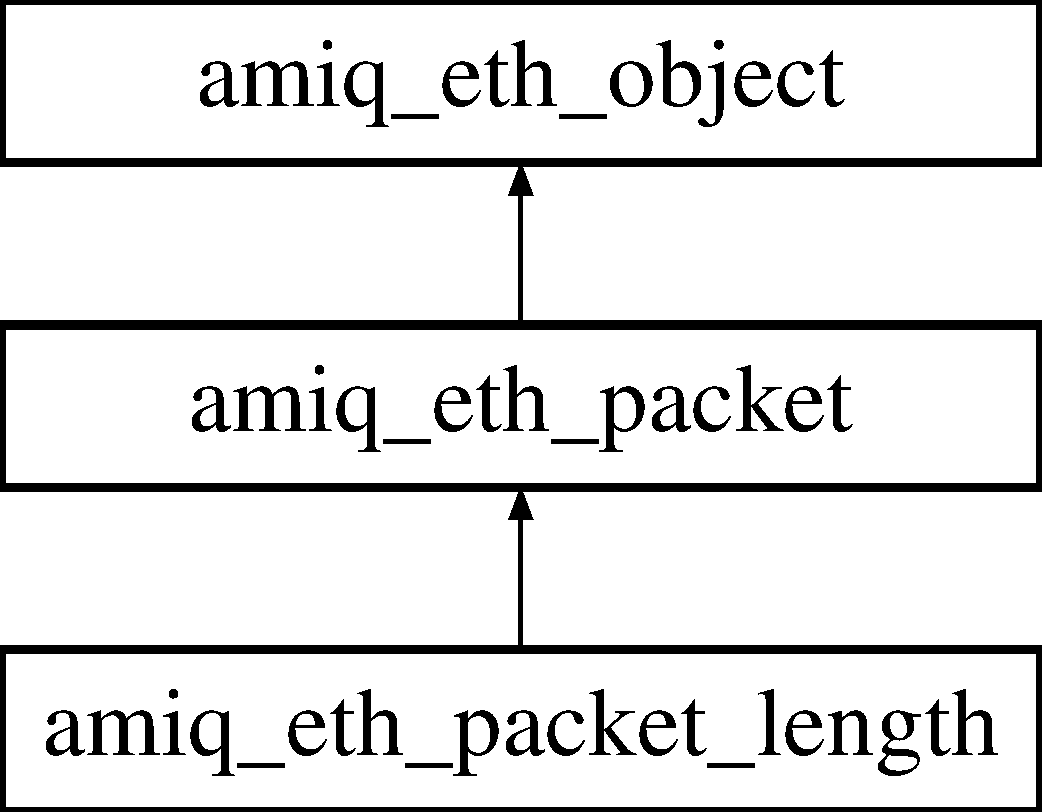
\includegraphics[height=3cm]{classamiq__eth__packet__length}
\end{center}
\end{figure}
\subsection*{Public Member Functions}
\begin{DoxyCompactItemize}
\item 
\hyperlink{classamiq__eth__packet__length_a7967fef155cea572ef45f46baaa2e9a4}{amiq\_\-eth\_\-packet\_\-length} ()
\item 
virtual \hyperlink{classamiq__eth__packet__length_aa58226b9a57fb5a13ed5914686d2e5c1}{$\sim$amiq\_\-eth\_\-packet\_\-length} ()
\item 
virtual void \hyperlink{classamiq__eth__packet__length_a2caccb08da11dbb3ab39178bc41bca75}{do\_\-print} (ostream \&out) const 
\item 
virtual void \hyperlink{classamiq__eth__packet__length_a0e4e4b570a84eda1274ff8f0e76b45df}{do\_\-pack} (\hyperlink{classamiq__eth__packer}{amiq\_\-eth\_\-packer} \&packer) const 
\item 
virtual void \hyperlink{classamiq__eth__packet__length_ab496b25828caaf23edd5fa6d4729c578}{do\_\-unpack} (\hyperlink{classamiq__eth__packer}{amiq\_\-eth\_\-packer} \&packer)
\end{DoxyCompactItemize}
\subsection*{Public Attributes}
\begin{DoxyCompactItemize}
\item 
\hyperlink{amiq__eth__types_8cpp_a4d2be172e6524c991fe389337947afc0}{amiq\_\-eth\_\-length\_\-type} \hyperlink{classamiq__eth__packet__length_aed41233fe35015c65e02b57a496e2072}{length\_\-type}
\item 
\hyperlink{amiq__eth__types_8cpp_a3595a0a508d433d383d3e5521fc0b723}{amiq\_\-eth\_\-data} $\ast$ \hyperlink{classamiq__eth__packet__length_a66584df88e48a4d67f104806d762636a}{payload}
\item 
\hyperlink{amiq__eth__types_8cpp_adb511dc715b55539c6abdad1de981a9f}{amiq\_\-eth\_\-fcs} \hyperlink{classamiq__eth__packet__length_a955aef311a4f2fb0e7d9f10aa756e68a}{fcs}
\end{DoxyCompactItemize}


\subsection{Detailed Description}


Definition at line 32 of file amiq\_\-eth\_\-packet\_\-length.cpp.

\subsection{Constructor \& Destructor Documentation}
\hypertarget{classamiq__eth__packet__length_a7967fef155cea572ef45f46baaa2e9a4}{
\index{amiq\_\-eth\_\-packet\_\-length@{amiq\_\-eth\_\-packet\_\-length}!amiq\_\-eth\_\-packet\_\-length@{amiq\_\-eth\_\-packet\_\-length}}
\index{amiq\_\-eth\_\-packet\_\-length@{amiq\_\-eth\_\-packet\_\-length}!amiq_eth_packet_length@{amiq\_\-eth\_\-packet\_\-length}}
\subsubsection[{amiq\_\-eth\_\-packet\_\-length}]{\setlength{\rightskip}{0pt plus 5cm}amiq\_\-eth\_\-packet\_\-length::amiq\_\-eth\_\-packet\_\-length ()\hspace{0.3cm}{\ttfamily  \mbox{[}inline\mbox{]}}}}
\label{classamiq__eth__packet__length_a7967fef155cea572ef45f46baaa2e9a4}


Definition at line 46 of file amiq\_\-eth\_\-packet\_\-length.cpp.

References NULL, and payload.\hypertarget{classamiq__eth__packet__length_aa58226b9a57fb5a13ed5914686d2e5c1}{
\index{amiq\_\-eth\_\-packet\_\-length@{amiq\_\-eth\_\-packet\_\-length}!$\sim$amiq\_\-eth\_\-packet\_\-length@{$\sim$amiq\_\-eth\_\-packet\_\-length}}
\index{$\sim$amiq\_\-eth\_\-packet\_\-length@{$\sim$amiq\_\-eth\_\-packet\_\-length}!amiq_eth_packet_length@{amiq\_\-eth\_\-packet\_\-length}}
\subsubsection[{$\sim$amiq\_\-eth\_\-packet\_\-length}]{\setlength{\rightskip}{0pt plus 5cm}virtual amiq\_\-eth\_\-packet\_\-length::$\sim$amiq\_\-eth\_\-packet\_\-length ()\hspace{0.3cm}{\ttfamily  \mbox{[}inline, virtual\mbox{]}}}}
\label{classamiq__eth__packet__length_aa58226b9a57fb5a13ed5914686d2e5c1}


Definition at line 51 of file amiq\_\-eth\_\-packet\_\-length.cpp.

References payload.

\subsection{Member Function Documentation}
\hypertarget{classamiq__eth__packet__length_a0e4e4b570a84eda1274ff8f0e76b45df}{
\index{amiq\_\-eth\_\-packet\_\-length@{amiq\_\-eth\_\-packet\_\-length}!do\_\-pack@{do\_\-pack}}
\index{do\_\-pack@{do\_\-pack}!amiq_eth_packet_length@{amiq\_\-eth\_\-packet\_\-length}}
\subsubsection[{do\_\-pack}]{\setlength{\rightskip}{0pt plus 5cm}virtual void amiq\_\-eth\_\-packet\_\-length::do\_\-pack ({\bf amiq\_\-eth\_\-packer} \& {\em packer}) const\hspace{0.3cm}{\ttfamily  \mbox{[}inline, virtual\mbox{]}}}}
\label{classamiq__eth__packet__length_a0e4e4b570a84eda1274ff8f0e76b45df}


Reimplemented from \hyperlink{classamiq__eth__packet_ab580d89fb44208f5a0fe31443619473e}{amiq\_\-eth\_\-packet}.

Definition at line 63 of file amiq\_\-eth\_\-packet\_\-length.cpp.

References amiq\_\-eth\_\-do\_\-pack(), fcs, length\_\-type, and payload.\hypertarget{classamiq__eth__packet__length_a2caccb08da11dbb3ab39178bc41bca75}{
\index{amiq\_\-eth\_\-packet\_\-length@{amiq\_\-eth\_\-packet\_\-length}!do\_\-print@{do\_\-print}}
\index{do\_\-print@{do\_\-print}!amiq_eth_packet_length@{amiq\_\-eth\_\-packet\_\-length}}
\subsubsection[{do\_\-print}]{\setlength{\rightskip}{0pt plus 5cm}virtual void amiq\_\-eth\_\-packet\_\-length::do\_\-print (ostream \& {\em out}) const\hspace{0.3cm}{\ttfamily  \mbox{[}inline, virtual\mbox{]}}}}
\label{classamiq__eth__packet__length_a2caccb08da11dbb3ab39178bc41bca75}


Reimplemented from \hyperlink{classamiq__eth__packet_aa179c700ae183f1b884a9222a73fed4e}{amiq\_\-eth\_\-packet}.

Definition at line 57 of file amiq\_\-eth\_\-packet\_\-length.cpp.\hypertarget{classamiq__eth__packet__length_ab496b25828caaf23edd5fa6d4729c578}{
\index{amiq\_\-eth\_\-packet\_\-length@{amiq\_\-eth\_\-packet\_\-length}!do\_\-unpack@{do\_\-unpack}}
\index{do\_\-unpack@{do\_\-unpack}!amiq_eth_packet_length@{amiq\_\-eth\_\-packet\_\-length}}
\subsubsection[{do\_\-unpack}]{\setlength{\rightskip}{0pt plus 5cm}virtual void amiq\_\-eth\_\-packet\_\-length::do\_\-unpack ({\bf amiq\_\-eth\_\-packer} \& {\em packer})\hspace{0.3cm}{\ttfamily  \mbox{[}inline, virtual\mbox{]}}}}
\label{classamiq__eth__packet__length_ab496b25828caaf23edd5fa6d4729c578}


Reimplemented from \hyperlink{classamiq__eth__packet_a909eb3860185125564fa530496ed1c9e}{amiq\_\-eth\_\-packet}.

Definition at line 77 of file amiq\_\-eth\_\-packet\_\-length.cpp.

References amiq\_\-eth\_\-do\_\-unpack(), fcs, length\_\-type, and payload.

\subsection{Member Data Documentation}
\hypertarget{classamiq__eth__packet__length_a955aef311a4f2fb0e7d9f10aa756e68a}{
\index{amiq\_\-eth\_\-packet\_\-length@{amiq\_\-eth\_\-packet\_\-length}!fcs@{fcs}}
\index{fcs@{fcs}!amiq_eth_packet_length@{amiq\_\-eth\_\-packet\_\-length}}
\subsubsection[{fcs}]{\setlength{\rightskip}{0pt plus 5cm}{\bf amiq\_\-eth\_\-fcs} {\bf amiq\_\-eth\_\-packet\_\-length::fcs}}}
\label{classamiq__eth__packet__length_a955aef311a4f2fb0e7d9f10aa756e68a}


Definition at line 43 of file amiq\_\-eth\_\-packet\_\-length.cpp.

Referenced by do\_\-pack(), and do\_\-unpack().\hypertarget{classamiq__eth__packet__length_aed41233fe35015c65e02b57a496e2072}{
\index{amiq\_\-eth\_\-packet\_\-length@{amiq\_\-eth\_\-packet\_\-length}!length\_\-type@{length\_\-type}}
\index{length\_\-type@{length\_\-type}!amiq_eth_packet_length@{amiq\_\-eth\_\-packet\_\-length}}
\subsubsection[{length\_\-type}]{\setlength{\rightskip}{0pt plus 5cm}{\bf amiq\_\-eth\_\-length\_\-type} {\bf amiq\_\-eth\_\-packet\_\-length::length\_\-type}}}
\label{classamiq__eth__packet__length_aed41233fe35015c65e02b57a496e2072}


Definition at line 37 of file amiq\_\-eth\_\-packet\_\-length.cpp.

Referenced by do\_\-pack(), and do\_\-unpack().\hypertarget{classamiq__eth__packet__length_a66584df88e48a4d67f104806d762636a}{
\index{amiq\_\-eth\_\-packet\_\-length@{amiq\_\-eth\_\-packet\_\-length}!payload@{payload}}
\index{payload@{payload}!amiq_eth_packet_length@{amiq\_\-eth\_\-packet\_\-length}}
\subsubsection[{payload}]{\setlength{\rightskip}{0pt plus 5cm}{\bf amiq\_\-eth\_\-data}$\ast$ {\bf amiq\_\-eth\_\-packet\_\-length::payload}}}
\label{classamiq__eth__packet__length_a66584df88e48a4d67f104806d762636a}


Definition at line 40 of file amiq\_\-eth\_\-packet\_\-length.cpp.

Referenced by amiq\_\-eth\_\-packet\_\-length(), do\_\-pack(), do\_\-unpack(), and $\sim$amiq\_\-eth\_\-packet\_\-length().

The documentation for this class was generated from the following file:\begin{DoxyCompactItemize}
\item 
/home/cristian.slav/work/amiq/projects/sv/amiq\_\-eth/sc/\hyperlink{amiq__eth__packet__length_8cpp}{amiq\_\-eth\_\-packet\_\-length.cpp}\end{DoxyCompactItemize}

\hypertarget{classamiq__eth__packet__magic}{
\section{amiq\_\-eth\_\-packet\_\-magic Class Reference}
\label{classamiq__eth__packet__magic}\index{amiq\_\-eth\_\-packet\_\-magic@{amiq\_\-eth\_\-packet\_\-magic}}
}
Inheritance diagram for amiq\_\-eth\_\-packet\_\-magic::\begin{figure}[H]
\begin{center}
\leavevmode
\includegraphics[height=4cm]{classamiq__eth__packet__magic}
\end{center}
\end{figure}
\subsection*{Public Member Functions}
\begin{DoxyCompactItemize}
\item 
\hyperlink{classamiq__eth__packet__magic_ad980d72550a76056113b94a6e2105123}{amiq\_\-eth\_\-packet\_\-magic} ()
\item 
virtual \hyperlink{classamiq__eth__packet__magic_a56f19042d3acfd4cd22d05b25962936f}{$\sim$amiq\_\-eth\_\-packet\_\-magic} ()
\item 
virtual void \hyperlink{classamiq__eth__packet__magic_aad43e3e40b85ee732b3e883b85a63ca6}{pack\_\-fcs} (\hyperlink{classamiq__eth__packer}{amiq\_\-eth\_\-packer} \&packer) const 
\item 
virtual void \hyperlink{classamiq__eth__packet__magic_ad026a187c1d882aa1698a3b0d4209472}{do\_\-pack} (\hyperlink{classamiq__eth__packer}{amiq\_\-eth\_\-packer} \&packer) const 
\item 
virtual void \hyperlink{classamiq__eth__packet__magic_a400a90ae523af44eb0c38ba64ea6afe7}{do\_\-unpack} (\hyperlink{classamiq__eth__packer}{amiq\_\-eth\_\-packer} \&packer)
\item 
virtual void \hyperlink{classamiq__eth__packet__magic_a0a40225ac5c36e70f413cd6d8ffd9a24}{do\_\-pack\_\-for\_\-fcs} (\hyperlink{classamiq__eth__packer}{amiq\_\-eth\_\-packer} \&packer) const 
\item 
virtual void \hyperlink{classamiq__eth__packet__magic_a57354d611adb80b1a8f4ad00c4f307a3}{do\_\-print} (ostream \&out) const 
\item 
virtual void \hyperlink{classamiq__eth__packet__magic_a88cbdc3d686e90941c250d758a72c8be}{set\_\-useful\_\-info\_\-in\_\-client\_\-data} ()
\item 
virtual void \hyperlink{classamiq__eth__packet__magic_aa9451a4b2d3566114694bd4a578759da}{get\_\-useful\_\-info\_\-from\_\-client\_\-data} ()
\item 
virtual tlm\_\-generic\_\-payload $\ast$ \hyperlink{classamiq__eth__packet__magic_adfe68e5b2702826b23d606caf90ab2bc}{to\_\-generic\_\-payload} () const 
\end{DoxyCompactItemize}
\subsection*{Public Attributes}
\begin{DoxyCompactItemize}
\item 
\hyperlink{amiq__eth__types_8cpp_a76a5a0c4430f7bd4f0773ac89fcc104a}{amiq\_\-eth\_\-address} \hyperlink{classamiq__eth__packet__magic_a637e45b53f846df836bf9cc3ac3dfcd6}{target\_\-mac}
\item 
unsigned int \hyperlink{classamiq__eth__packet__magic_a9886d0fb22aecb6ff6223bc527391a46}{password\_\-size}
\item 
\hyperlink{amiq__eth__types_8cpp_a3595a0a508d433d383d3e5521fc0b723}{amiq\_\-eth\_\-data} $\ast$ \hyperlink{classamiq__eth__packet__magic_a42adfe3e292a6b67e466ded58dfa7d1c}{password}
\item 
\hyperlink{amiq__eth__types_8cpp_a91e895e78bf9f23c2cab9db2fb280e8b}{amiq\_\-eth\_\-jumbo\_\-client\_\-data\_\-size} \hyperlink{classamiq__eth__packet__magic_abc186b414e871bb0b06544bfb4bea774}{client\_\-data\_\-size}
\item 
\hyperlink{amiq__eth__types_8cpp_a3595a0a508d433d383d3e5521fc0b723}{amiq\_\-eth\_\-data} $\ast$ \hyperlink{classamiq__eth__packet__magic_a1f725ceba2f857032fbae819b7af409f}{client\_\-data}
\item 
\hyperlink{amiq__eth__types_8cpp_adb511dc715b55539c6abdad1de981a9f}{amiq\_\-eth\_\-fcs} \hyperlink{classamiq__eth__packet__magic_af8870f1b03256d0bed2dedc39a74d0f5}{fcs}
\item 
int \hyperlink{classamiq__eth__packet__magic_adf2528cb7352ff0a1876232483803a4f}{synch\_\-stream\_\-starting\_\-index}
\end{DoxyCompactItemize}


\subsection{Detailed Description}


Definition at line 33 of file amiq\_\-eth\_\-packet\_\-magic.cpp.

\subsection{Constructor \& Destructor Documentation}
\hypertarget{classamiq__eth__packet__magic_ad980d72550a76056113b94a6e2105123}{
\index{amiq\_\-eth\_\-packet\_\-magic@{amiq\_\-eth\_\-packet\_\-magic}!amiq\_\-eth\_\-packet\_\-magic@{amiq\_\-eth\_\-packet\_\-magic}}
\index{amiq\_\-eth\_\-packet\_\-magic@{amiq\_\-eth\_\-packet\_\-magic}!amiq_eth_packet_magic@{amiq\_\-eth\_\-packet\_\-magic}}
\subsubsection[{amiq\_\-eth\_\-packet\_\-magic}]{\setlength{\rightskip}{0pt plus 5cm}amiq\_\-eth\_\-packet\_\-magic::amiq\_\-eth\_\-packet\_\-magic ()\hspace{0.3cm}{\ttfamily  \mbox{[}inline\mbox{]}}}}
\label{classamiq__eth__packet__magic_ad980d72550a76056113b94a6e2105123}


Definition at line 59 of file amiq\_\-eth\_\-packet\_\-magic.cpp.

References client\_\-data, NULL, password, and synch\_\-stream\_\-starting\_\-index.\hypertarget{classamiq__eth__packet__magic_a56f19042d3acfd4cd22d05b25962936f}{
\index{amiq\_\-eth\_\-packet\_\-magic@{amiq\_\-eth\_\-packet\_\-magic}!$\sim$amiq\_\-eth\_\-packet\_\-magic@{$\sim$amiq\_\-eth\_\-packet\_\-magic}}
\index{$\sim$amiq\_\-eth\_\-packet\_\-magic@{$\sim$amiq\_\-eth\_\-packet\_\-magic}!amiq_eth_packet_magic@{amiq\_\-eth\_\-packet\_\-magic}}
\subsubsection[{$\sim$amiq\_\-eth\_\-packet\_\-magic}]{\setlength{\rightskip}{0pt plus 5cm}virtual amiq\_\-eth\_\-packet\_\-magic::$\sim$amiq\_\-eth\_\-packet\_\-magic ()\hspace{0.3cm}{\ttfamily  \mbox{[}inline, virtual\mbox{]}}}}
\label{classamiq__eth__packet__magic_a56f19042d3acfd4cd22d05b25962936f}


Definition at line 66 of file amiq\_\-eth\_\-packet\_\-magic.cpp.

References client\_\-data, NULL, and password.

\subsection{Member Function Documentation}
\hypertarget{classamiq__eth__packet__magic_ad026a187c1d882aa1698a3b0d4209472}{
\index{amiq\_\-eth\_\-packet\_\-magic@{amiq\_\-eth\_\-packet\_\-magic}!do\_\-pack@{do\_\-pack}}
\index{do\_\-pack@{do\_\-pack}!amiq_eth_packet_magic@{amiq\_\-eth\_\-packet\_\-magic}}
\subsubsection[{do\_\-pack}]{\setlength{\rightskip}{0pt plus 5cm}virtual void amiq\_\-eth\_\-packet\_\-magic::do\_\-pack ({\bf amiq\_\-eth\_\-packer} \& {\em packer}) const\hspace{0.3cm}{\ttfamily  \mbox{[}inline, virtual\mbox{]}}}}
\label{classamiq__eth__packet__magic_ad026a187c1d882aa1698a3b0d4209472}


Reimplemented from \hyperlink{classamiq__eth__packet__ether__type_a62fe5f26a466f0bd0045599b89aa6926}{amiq\_\-eth\_\-packet\_\-ether\_\-type}.

Definition at line 79 of file amiq\_\-eth\_\-packet\_\-magic.cpp.

References amiq\_\-eth\_\-do\_\-pack(), client\_\-data, client\_\-data\_\-size, and pack\_\-fcs().\hypertarget{classamiq__eth__packet__magic_a0a40225ac5c36e70f413cd6d8ffd9a24}{
\index{amiq\_\-eth\_\-packet\_\-magic@{amiq\_\-eth\_\-packet\_\-magic}!do\_\-pack\_\-for\_\-fcs@{do\_\-pack\_\-for\_\-fcs}}
\index{do\_\-pack\_\-for\_\-fcs@{do\_\-pack\_\-for\_\-fcs}!amiq_eth_packet_magic@{amiq\_\-eth\_\-packet\_\-magic}}
\subsubsection[{do\_\-pack\_\-for\_\-fcs}]{\setlength{\rightskip}{0pt plus 5cm}virtual void amiq\_\-eth\_\-packet\_\-magic::do\_\-pack\_\-for\_\-fcs ({\bf amiq\_\-eth\_\-packer} \& {\em packer}) const\hspace{0.3cm}{\ttfamily  \mbox{[}inline, virtual\mbox{]}}}}
\label{classamiq__eth__packet__magic_a0a40225ac5c36e70f413cd6d8ffd9a24}


Reimplemented from \hyperlink{classamiq__eth__packet__ether__type_aaa85cf778650e1c1b377392a975cb7bc}{amiq\_\-eth\_\-packet\_\-ether\_\-type}.

Definition at line 115 of file amiq\_\-eth\_\-packet\_\-magic.cpp.

References amiq\_\-eth\_\-do\_\-pack(), client\_\-data, and client\_\-data\_\-size.\hypertarget{classamiq__eth__packet__magic_a57354d611adb80b1a8f4ad00c4f307a3}{
\index{amiq\_\-eth\_\-packet\_\-magic@{amiq\_\-eth\_\-packet\_\-magic}!do\_\-print@{do\_\-print}}
\index{do\_\-print@{do\_\-print}!amiq_eth_packet_magic@{amiq\_\-eth\_\-packet\_\-magic}}
\subsubsection[{do\_\-print}]{\setlength{\rightskip}{0pt plus 5cm}virtual void amiq\_\-eth\_\-packet\_\-magic::do\_\-print (ostream \& {\em out}) const\hspace{0.3cm}{\ttfamily  \mbox{[}inline, virtual\mbox{]}}}}
\label{classamiq__eth__packet__magic_a57354d611adb80b1a8f4ad00c4f307a3}


Reimplemented from \hyperlink{classamiq__eth__packet__ether__type_a9b2852fa1aaf278138fde2232e446f63}{amiq\_\-eth\_\-packet\_\-ether\_\-type}.

Definition at line 127 of file amiq\_\-eth\_\-packet\_\-magic.cpp.

References AMIQ\_\-ETH\_\-FIELD\_\-SEPARATOR, client\_\-data\_\-size, fcs, amiq\_\-eth\_\-packet::get\_\-correct\_\-fcs(), synch\_\-stream\_\-starting\_\-index, and target\_\-mac.

Referenced by get\_\-useful\_\-info\_\-from\_\-client\_\-data().\hypertarget{classamiq__eth__packet__magic_a400a90ae523af44eb0c38ba64ea6afe7}{
\index{amiq\_\-eth\_\-packet\_\-magic@{amiq\_\-eth\_\-packet\_\-magic}!do\_\-unpack@{do\_\-unpack}}
\index{do\_\-unpack@{do\_\-unpack}!amiq_eth_packet_magic@{amiq\_\-eth\_\-packet\_\-magic}}
\subsubsection[{do\_\-unpack}]{\setlength{\rightskip}{0pt plus 5cm}virtual void amiq\_\-eth\_\-packet\_\-magic::do\_\-unpack ({\bf amiq\_\-eth\_\-packer} \& {\em packer})\hspace{0.3cm}{\ttfamily  \mbox{[}inline, virtual\mbox{]}}}}
\label{classamiq__eth__packet__magic_a400a90ae523af44eb0c38ba64ea6afe7}


Reimplemented from \hyperlink{classamiq__eth__packet__ether__type_a0c86ef80c46bbed384739b23e5efb0ef}{amiq\_\-eth\_\-packet\_\-ether\_\-type}.

Definition at line 95 of file amiq\_\-eth\_\-packet\_\-magic.cpp.

References amiq\_\-eth\_\-do\_\-unpack(), client\_\-data, client\_\-data\_\-size, fcs, and get\_\-useful\_\-info\_\-from\_\-client\_\-data().\hypertarget{classamiq__eth__packet__magic_aa9451a4b2d3566114694bd4a578759da}{
\index{amiq\_\-eth\_\-packet\_\-magic@{amiq\_\-eth\_\-packet\_\-magic}!get\_\-useful\_\-info\_\-from\_\-client\_\-data@{get\_\-useful\_\-info\_\-from\_\-client\_\-data}}
\index{get\_\-useful\_\-info\_\-from\_\-client\_\-data@{get\_\-useful\_\-info\_\-from\_\-client\_\-data}!amiq_eth_packet_magic@{amiq\_\-eth\_\-packet\_\-magic}}
\subsubsection[{get\_\-useful\_\-info\_\-from\_\-client\_\-data}]{\setlength{\rightskip}{0pt plus 5cm}virtual void amiq\_\-eth\_\-packet\_\-magic::get\_\-useful\_\-info\_\-from\_\-client\_\-data ()\hspace{0.3cm}{\ttfamily  \mbox{[}inline, virtual\mbox{]}}}}
\label{classamiq__eth__packet__magic_aa9451a4b2d3566114694bd4a578759da}


Definition at line 187 of file amiq\_\-eth\_\-packet\_\-magic.cpp.

References AMIQ\_\-ETH\_\-ADDRESS\_\-WIDTH, amiq\_\-eth\_\-do\_\-pack(), AMIQ\_\-ETH\_\-MAGIC\_\-PACKET\_\-SYNCH\_\-STREAM, AMIQ\_\-ETH\_\-MAGIC\_\-PACKET\_\-SYNCH\_\-STREAM\_\-WIDTH, AMIQ\_\-ETH\_\-MAGIC\_\-PACKET\_\-TARGET\_\-MAC\_\-REPETITIONS, client\_\-data, client\_\-data\_\-size, do\_\-print(), amiq\_\-eth\_\-packer::get\_\-bytes(), password, password\_\-size, amiq\_\-eth\_\-packer::reset(), synch\_\-stream\_\-starting\_\-index, and target\_\-mac.

Referenced by do\_\-unpack().\hypertarget{classamiq__eth__packet__magic_aad43e3e40b85ee732b3e883b85a63ca6}{
\index{amiq\_\-eth\_\-packet\_\-magic@{amiq\_\-eth\_\-packet\_\-magic}!pack\_\-fcs@{pack\_\-fcs}}
\index{pack\_\-fcs@{pack\_\-fcs}!amiq_eth_packet_magic@{amiq\_\-eth\_\-packet\_\-magic}}
\subsubsection[{pack\_\-fcs}]{\setlength{\rightskip}{0pt plus 5cm}virtual void amiq\_\-eth\_\-packet\_\-magic::pack\_\-fcs ({\bf amiq\_\-eth\_\-packer} \& {\em packer}) const\hspace{0.3cm}{\ttfamily  \mbox{[}inline, virtual\mbox{]}}}}
\label{classamiq__eth__packet__magic_aad43e3e40b85ee732b3e883b85a63ca6}


Definition at line 73 of file amiq\_\-eth\_\-packet\_\-magic.cpp.

References amiq\_\-eth\_\-do\_\-pack(), and fcs.

Referenced by do\_\-pack().\hypertarget{classamiq__eth__packet__magic_a88cbdc3d686e90941c250d758a72c8be}{
\index{amiq\_\-eth\_\-packet\_\-magic@{amiq\_\-eth\_\-packet\_\-magic}!set\_\-useful\_\-info\_\-in\_\-client\_\-data@{set\_\-useful\_\-info\_\-in\_\-client\_\-data}}
\index{set\_\-useful\_\-info\_\-in\_\-client\_\-data@{set\_\-useful\_\-info\_\-in\_\-client\_\-data}!amiq_eth_packet_magic@{amiq\_\-eth\_\-packet\_\-magic}}
\subsubsection[{set\_\-useful\_\-info\_\-in\_\-client\_\-data}]{\setlength{\rightskip}{0pt plus 5cm}virtual void amiq\_\-eth\_\-packet\_\-magic::set\_\-useful\_\-info\_\-in\_\-client\_\-data ()\hspace{0.3cm}{\ttfamily  \mbox{[}inline, virtual\mbox{]}}}}
\label{classamiq__eth__packet__magic_a88cbdc3d686e90941c250d758a72c8be}


Definition at line 148 of file amiq\_\-eth\_\-packet\_\-magic.cpp.

References AMIQ\_\-ETH\_\-ADDRESS\_\-WIDTH, amiq\_\-eth\_\-do\_\-pack(), AMIQ\_\-ETH\_\-MAGIC\_\-PACKET\_\-SYNCH\_\-STREAM, AMIQ\_\-ETH\_\-MAGIC\_\-PACKET\_\-SYNCH\_\-STREAM\_\-WIDTH, AMIQ\_\-ETH\_\-MAGIC\_\-PACKET\_\-TARGET\_\-MAC\_\-REPETITIONS, client\_\-data, amiq\_\-eth\_\-packer::get\_\-bytes(), amiq\_\-eth\_\-packer::reset(), synch\_\-stream\_\-starting\_\-index, and target\_\-mac.\hypertarget{classamiq__eth__packet__magic_adfe68e5b2702826b23d606caf90ab2bc}{
\index{amiq\_\-eth\_\-packet\_\-magic@{amiq\_\-eth\_\-packet\_\-magic}!to\_\-generic\_\-payload@{to\_\-generic\_\-payload}}
\index{to\_\-generic\_\-payload@{to\_\-generic\_\-payload}!amiq_eth_packet_magic@{amiq\_\-eth\_\-packet\_\-magic}}
\subsubsection[{to\_\-generic\_\-payload}]{\setlength{\rightskip}{0pt plus 5cm}virtual tlm\_\-generic\_\-payload$\ast$ amiq\_\-eth\_\-packet\_\-magic::to\_\-generic\_\-payload () const\hspace{0.3cm}{\ttfamily  \mbox{[}inline, virtual\mbox{]}}}}
\label{classamiq__eth__packet__magic_adfe68e5b2702826b23d606caf90ab2bc}


Reimplemented from \hyperlink{classamiq__eth__packet_a6dd92751d8172eeaa347d71bb415b0d5}{amiq\_\-eth\_\-packet}.

Definition at line 306 of file amiq\_\-eth\_\-packet\_\-magic.cpp.

References AMIQ\_\-ETH\_\-PACKET\_\-MAGIC\_\-CODE.

\subsection{Member Data Documentation}
\hypertarget{classamiq__eth__packet__magic_a1f725ceba2f857032fbae819b7af409f}{
\index{amiq\_\-eth\_\-packet\_\-magic@{amiq\_\-eth\_\-packet\_\-magic}!client\_\-data@{client\_\-data}}
\index{client\_\-data@{client\_\-data}!amiq_eth_packet_magic@{amiq\_\-eth\_\-packet\_\-magic}}
\subsubsection[{client\_\-data}]{\setlength{\rightskip}{0pt plus 5cm}{\bf amiq\_\-eth\_\-data}$\ast$ {\bf amiq\_\-eth\_\-packet\_\-magic::client\_\-data}}}
\label{classamiq__eth__packet__magic_a1f725ceba2f857032fbae819b7af409f}


Definition at line 50 of file amiq\_\-eth\_\-packet\_\-magic.cpp.

Referenced by amiq\_\-eth\_\-packet\_\-magic(), do\_\-pack(), do\_\-pack\_\-for\_\-fcs(), do\_\-unpack(), get\_\-useful\_\-info\_\-from\_\-client\_\-data(), set\_\-useful\_\-info\_\-in\_\-client\_\-data(), and $\sim$amiq\_\-eth\_\-packet\_\-magic().\hypertarget{classamiq__eth__packet__magic_abc186b414e871bb0b06544bfb4bea774}{
\index{amiq\_\-eth\_\-packet\_\-magic@{amiq\_\-eth\_\-packet\_\-magic}!client\_\-data\_\-size@{client\_\-data\_\-size}}
\index{client\_\-data\_\-size@{client\_\-data\_\-size}!amiq_eth_packet_magic@{amiq\_\-eth\_\-packet\_\-magic}}
\subsubsection[{client\_\-data\_\-size}]{\setlength{\rightskip}{0pt plus 5cm}{\bf amiq\_\-eth\_\-jumbo\_\-client\_\-data\_\-size} {\bf amiq\_\-eth\_\-packet\_\-magic::client\_\-data\_\-size}}}
\label{classamiq__eth__packet__magic_abc186b414e871bb0b06544bfb4bea774}


Definition at line 47 of file amiq\_\-eth\_\-packet\_\-magic.cpp.

Referenced by do\_\-pack(), do\_\-pack\_\-for\_\-fcs(), do\_\-print(), do\_\-unpack(), and get\_\-useful\_\-info\_\-from\_\-client\_\-data().\hypertarget{classamiq__eth__packet__magic_af8870f1b03256d0bed2dedc39a74d0f5}{
\index{amiq\_\-eth\_\-packet\_\-magic@{amiq\_\-eth\_\-packet\_\-magic}!fcs@{fcs}}
\index{fcs@{fcs}!amiq_eth_packet_magic@{amiq\_\-eth\_\-packet\_\-magic}}
\subsubsection[{fcs}]{\setlength{\rightskip}{0pt plus 5cm}{\bf amiq\_\-eth\_\-fcs} {\bf amiq\_\-eth\_\-packet\_\-magic::fcs}}}
\label{classamiq__eth__packet__magic_af8870f1b03256d0bed2dedc39a74d0f5}


Definition at line 53 of file amiq\_\-eth\_\-packet\_\-magic.cpp.

Referenced by do\_\-print(), do\_\-unpack(), and pack\_\-fcs().\hypertarget{classamiq__eth__packet__magic_a42adfe3e292a6b67e466ded58dfa7d1c}{
\index{amiq\_\-eth\_\-packet\_\-magic@{amiq\_\-eth\_\-packet\_\-magic}!password@{password}}
\index{password@{password}!amiq_eth_packet_magic@{amiq\_\-eth\_\-packet\_\-magic}}
\subsubsection[{password}]{\setlength{\rightskip}{0pt plus 5cm}{\bf amiq\_\-eth\_\-data}$\ast$ {\bf amiq\_\-eth\_\-packet\_\-magic::password}}}
\label{classamiq__eth__packet__magic_a42adfe3e292a6b67e466ded58dfa7d1c}


Definition at line 44 of file amiq\_\-eth\_\-packet\_\-magic.cpp.

Referenced by amiq\_\-eth\_\-packet\_\-magic(), get\_\-useful\_\-info\_\-from\_\-client\_\-data(), and $\sim$amiq\_\-eth\_\-packet\_\-magic().\hypertarget{classamiq__eth__packet__magic_a9886d0fb22aecb6ff6223bc527391a46}{
\index{amiq\_\-eth\_\-packet\_\-magic@{amiq\_\-eth\_\-packet\_\-magic}!password\_\-size@{password\_\-size}}
\index{password\_\-size@{password\_\-size}!amiq_eth_packet_magic@{amiq\_\-eth\_\-packet\_\-magic}}
\subsubsection[{password\_\-size}]{\setlength{\rightskip}{0pt plus 5cm}unsigned int {\bf amiq\_\-eth\_\-packet\_\-magic::password\_\-size}}}
\label{classamiq__eth__packet__magic_a9886d0fb22aecb6ff6223bc527391a46}


Definition at line 41 of file amiq\_\-eth\_\-packet\_\-magic.cpp.

Referenced by get\_\-useful\_\-info\_\-from\_\-client\_\-data().\hypertarget{classamiq__eth__packet__magic_adf2528cb7352ff0a1876232483803a4f}{
\index{amiq\_\-eth\_\-packet\_\-magic@{amiq\_\-eth\_\-packet\_\-magic}!synch\_\-stream\_\-starting\_\-index@{synch\_\-stream\_\-starting\_\-index}}
\index{synch\_\-stream\_\-starting\_\-index@{synch\_\-stream\_\-starting\_\-index}!amiq_eth_packet_magic@{amiq\_\-eth\_\-packet\_\-magic}}
\subsubsection[{synch\_\-stream\_\-starting\_\-index}]{\setlength{\rightskip}{0pt plus 5cm}int {\bf amiq\_\-eth\_\-packet\_\-magic::synch\_\-stream\_\-starting\_\-index}}}
\label{classamiq__eth__packet__magic_adf2528cb7352ff0a1876232483803a4f}


Definition at line 56 of file amiq\_\-eth\_\-packet\_\-magic.cpp.

Referenced by amiq\_\-eth\_\-packet\_\-magic(), do\_\-print(), get\_\-useful\_\-info\_\-from\_\-client\_\-data(), and set\_\-useful\_\-info\_\-in\_\-client\_\-data().\hypertarget{classamiq__eth__packet__magic_a637e45b53f846df836bf9cc3ac3dfcd6}{
\index{amiq\_\-eth\_\-packet\_\-magic@{amiq\_\-eth\_\-packet\_\-magic}!target\_\-mac@{target\_\-mac}}
\index{target\_\-mac@{target\_\-mac}!amiq_eth_packet_magic@{amiq\_\-eth\_\-packet\_\-magic}}
\subsubsection[{target\_\-mac}]{\setlength{\rightskip}{0pt plus 5cm}{\bf amiq\_\-eth\_\-address} {\bf amiq\_\-eth\_\-packet\_\-magic::target\_\-mac}}}
\label{classamiq__eth__packet__magic_a637e45b53f846df836bf9cc3ac3dfcd6}


Definition at line 38 of file amiq\_\-eth\_\-packet\_\-magic.cpp.

Referenced by do\_\-print(), get\_\-useful\_\-info\_\-from\_\-client\_\-data(), and set\_\-useful\_\-info\_\-in\_\-client\_\-data().

The documentation for this class was generated from the following file:\begin{DoxyCompactItemize}
\item 
/home/cristian.slav/work/amiq/projects/sv/amiq\_\-eth/sc/\hyperlink{amiq__eth__packet__magic_8cpp}{amiq\_\-eth\_\-packet\_\-magic.cpp}\end{DoxyCompactItemize}

\hypertarget{classamiq__eth__packet__pause}{
\section{amiq\_\-eth\_\-packet\_\-pause Class Reference}
\label{classamiq__eth__packet__pause}\index{amiq\_\-eth\_\-packet\_\-pause@{amiq\_\-eth\_\-packet\_\-pause}}
}
Inheritance diagram for amiq\_\-eth\_\-packet\_\-pause::\begin{figure}[H]
\begin{center}
\leavevmode
\includegraphics[height=4cm]{classamiq__eth__packet__pause}
\end{center}
\end{figure}
\subsection*{Public Member Functions}
\begin{DoxyCompactItemize}
\item 
\hyperlink{classamiq__eth__packet__pause_ade911eec6984347c30f8b537b585c095}{amiq\_\-eth\_\-packet\_\-pause} ()
\item 
virtual \hyperlink{classamiq__eth__packet__pause_abe069c9121e346b2fbbc5aa693ab6a8d}{$\sim$amiq\_\-eth\_\-packet\_\-pause} ()
\item 
virtual void \hyperlink{classamiq__eth__packet__pause_a7ea960bd9c079375b0d4cd72a762d695}{do\_\-print} (ostream \&out) const 
\item 
virtual void \hyperlink{classamiq__eth__packet__pause_aaea61c8cafc5274eac5d2b5428876868}{do\_\-pack} (\hyperlink{classamiq__eth__packer}{amiq\_\-eth\_\-packer} \&packer) const 
\item 
virtual void \hyperlink{classamiq__eth__packet__pause_aa458964a73aa61bca99cb30ffa56f54c}{do\_\-unpack} (\hyperlink{classamiq__eth__packer}{amiq\_\-eth\_\-packer} \&packer)
\item 
virtual tlm\_\-generic\_\-payload $\ast$ \hyperlink{classamiq__eth__packet__pause_ab59bd7087700e15e79018f72d809d76a}{to\_\-generic\_\-payload} () const 
\end{DoxyCompactItemize}
\subsection*{Public Attributes}
\begin{DoxyCompactItemize}
\item 
\hyperlink{amiq__eth__types_8cpp_a882c4ca2cfd45ca7e4ab471fbaf6f348}{amiq\_\-eth\_\-pause\_\-opcode} \hyperlink{classamiq__eth__packet__pause_a31d48860ec5bc33e5e3c76a88a5cbd94}{pause\_\-opcode}
\item 
\hyperlink{amiq__eth__types_8cpp_a9506f5917bf0b1e03bd6946e62cc4a55}{amiq\_\-eth\_\-pause\_\-parameter} \hyperlink{classamiq__eth__packet__pause_ab767bf1d61f35e59a74babfe730ffe20}{pause\_\-parameter}
\item 
\hyperlink{amiq__eth__types_8cpp_a3595a0a508d433d383d3e5521fc0b723}{amiq\_\-eth\_\-data} $\ast$ \hyperlink{classamiq__eth__packet__pause_a23b5341742ff52a6144b1088cfe86ff8}{pad}
\item 
\hyperlink{amiq__eth__types_8cpp_adb511dc715b55539c6abdad1de981a9f}{amiq\_\-eth\_\-fcs} \hyperlink{classamiq__eth__packet__pause_a2ea030b909dafbd1470053eb13960eaa}{fcs}
\item 
unsigned int \hyperlink{classamiq__eth__packet__pause_ab2323424453362f82d9fc86ee9667e46}{pad\_\-size}
\end{DoxyCompactItemize}


\subsection{Detailed Description}


Definition at line 30 of file amiq\_\-eth\_\-packet\_\-pause.cpp.

\subsection{Constructor \& Destructor Documentation}
\hypertarget{classamiq__eth__packet__pause_ade911eec6984347c30f8b537b585c095}{
\index{amiq\_\-eth\_\-packet\_\-pause@{amiq\_\-eth\_\-packet\_\-pause}!amiq\_\-eth\_\-packet\_\-pause@{amiq\_\-eth\_\-packet\_\-pause}}
\index{amiq\_\-eth\_\-packet\_\-pause@{amiq\_\-eth\_\-packet\_\-pause}!amiq_eth_packet_pause@{amiq\_\-eth\_\-packet\_\-pause}}
\subsubsection[{amiq\_\-eth\_\-packet\_\-pause}]{\setlength{\rightskip}{0pt plus 5cm}amiq\_\-eth\_\-packet\_\-pause::amiq\_\-eth\_\-packet\_\-pause ()\hspace{0.3cm}{\ttfamily  \mbox{[}inline\mbox{]}}}}
\label{classamiq__eth__packet__pause_ade911eec6984347c30f8b537b585c095}


Definition at line 46 of file amiq\_\-eth\_\-packet\_\-pause.cpp.

References AMIQ\_\-ETH\_\-DATA\_\-WIDTH, AMIQ\_\-ETH\_\-PAUSE\_\-OPCODE, AMIQ\_\-ETH\_\-PAUSE\_\-OPCODE\_\-WIDTH, AMIQ\_\-ETH\_\-PAUSE\_\-PACKET\_\-DESTINATION\_\-ADDRESS, AMIQ\_\-ETH\_\-PAUSE\_\-PARAMETER\_\-WIDTH, AMIQ\_\-ETH\_\-PAYLOAD\_\-SIZE\_\-MIN, amiq\_\-eth\_\-packet::destination\_\-address, amiq\_\-eth\_\-packet\_\-ether\_\-type::ether\_\-type, NULL, pad, pad\_\-size, pause\_\-opcode, and SC\_\-AMIQ\_\-ETH\_\-MAC\_\-CONTROL.\hypertarget{classamiq__eth__packet__pause_abe069c9121e346b2fbbc5aa693ab6a8d}{
\index{amiq\_\-eth\_\-packet\_\-pause@{amiq\_\-eth\_\-packet\_\-pause}!$\sim$amiq\_\-eth\_\-packet\_\-pause@{$\sim$amiq\_\-eth\_\-packet\_\-pause}}
\index{$\sim$amiq\_\-eth\_\-packet\_\-pause@{$\sim$amiq\_\-eth\_\-packet\_\-pause}!amiq_eth_packet_pause@{amiq\_\-eth\_\-packet\_\-pause}}
\subsubsection[{$\sim$amiq\_\-eth\_\-packet\_\-pause}]{\setlength{\rightskip}{0pt plus 5cm}virtual amiq\_\-eth\_\-packet\_\-pause::$\sim$amiq\_\-eth\_\-packet\_\-pause ()\hspace{0.3cm}{\ttfamily  \mbox{[}inline, virtual\mbox{]}}}}
\label{classamiq__eth__packet__pause_abe069c9121e346b2fbbc5aa693ab6a8d}


Definition at line 59 of file amiq\_\-eth\_\-packet\_\-pause.cpp.

\subsection{Member Function Documentation}
\hypertarget{classamiq__eth__packet__pause_aaea61c8cafc5274eac5d2b5428876868}{
\index{amiq\_\-eth\_\-packet\_\-pause@{amiq\_\-eth\_\-packet\_\-pause}!do\_\-pack@{do\_\-pack}}
\index{do\_\-pack@{do\_\-pack}!amiq_eth_packet_pause@{amiq\_\-eth\_\-packet\_\-pause}}
\subsubsection[{do\_\-pack}]{\setlength{\rightskip}{0pt plus 5cm}virtual void amiq\_\-eth\_\-packet\_\-pause::do\_\-pack ({\bf amiq\_\-eth\_\-packer} \& {\em packer}) const\hspace{0.3cm}{\ttfamily  \mbox{[}inline, virtual\mbox{]}}}}
\label{classamiq__eth__packet__pause_aaea61c8cafc5274eac5d2b5428876868}


Reimplemented from \hyperlink{classamiq__eth__packet__ether__type_a62fe5f26a466f0bd0045599b89aa6926}{amiq\_\-eth\_\-packet\_\-ether\_\-type}.

Definition at line 75 of file amiq\_\-eth\_\-packet\_\-pause.cpp.

References amiq\_\-eth\_\-do\_\-pack(), fcs, pad, pad\_\-size, pause\_\-opcode, and pause\_\-parameter.\hypertarget{classamiq__eth__packet__pause_a7ea960bd9c079375b0d4cd72a762d695}{
\index{amiq\_\-eth\_\-packet\_\-pause@{amiq\_\-eth\_\-packet\_\-pause}!do\_\-print@{do\_\-print}}
\index{do\_\-print@{do\_\-print}!amiq_eth_packet_pause@{amiq\_\-eth\_\-packet\_\-pause}}
\subsubsection[{do\_\-print}]{\setlength{\rightskip}{0pt plus 5cm}virtual void amiq\_\-eth\_\-packet\_\-pause::do\_\-print (ostream \& {\em out}) const\hspace{0.3cm}{\ttfamily  \mbox{[}inline, virtual\mbox{]}}}}
\label{classamiq__eth__packet__pause_a7ea960bd9c079375b0d4cd72a762d695}


Reimplemented from \hyperlink{classamiq__eth__packet__ether__type_a9b2852fa1aaf278138fde2232e446f63}{amiq\_\-eth\_\-packet\_\-ether\_\-type}.

Definition at line 64 of file amiq\_\-eth\_\-packet\_\-pause.cpp.

References AMIQ\_\-ETH\_\-FIELD\_\-SEPARATOR, fcs, pad\_\-size, pause\_\-opcode, and pause\_\-parameter.\hypertarget{classamiq__eth__packet__pause_aa458964a73aa61bca99cb30ffa56f54c}{
\index{amiq\_\-eth\_\-packet\_\-pause@{amiq\_\-eth\_\-packet\_\-pause}!do\_\-unpack@{do\_\-unpack}}
\index{do\_\-unpack@{do\_\-unpack}!amiq_eth_packet_pause@{amiq\_\-eth\_\-packet\_\-pause}}
\subsubsection[{do\_\-unpack}]{\setlength{\rightskip}{0pt plus 5cm}virtual void amiq\_\-eth\_\-packet\_\-pause::do\_\-unpack ({\bf amiq\_\-eth\_\-packer} \& {\em packer})\hspace{0.3cm}{\ttfamily  \mbox{[}inline, virtual\mbox{]}}}}
\label{classamiq__eth__packet__pause_aa458964a73aa61bca99cb30ffa56f54c}


Reimplemented from \hyperlink{classamiq__eth__packet__ether__type_a0c86ef80c46bbed384739b23e5efb0ef}{amiq\_\-eth\_\-packet\_\-ether\_\-type}.

Definition at line 91 of file amiq\_\-eth\_\-packet\_\-pause.cpp.

References amiq\_\-eth\_\-do\_\-unpack(), fcs, pad, pad\_\-size, pause\_\-opcode, and pause\_\-parameter.\hypertarget{classamiq__eth__packet__pause_ab59bd7087700e15e79018f72d809d76a}{
\index{amiq\_\-eth\_\-packet\_\-pause@{amiq\_\-eth\_\-packet\_\-pause}!to\_\-generic\_\-payload@{to\_\-generic\_\-payload}}
\index{to\_\-generic\_\-payload@{to\_\-generic\_\-payload}!amiq_eth_packet_pause@{amiq\_\-eth\_\-packet\_\-pause}}
\subsubsection[{to\_\-generic\_\-payload}]{\setlength{\rightskip}{0pt plus 5cm}virtual tlm\_\-generic\_\-payload$\ast$ amiq\_\-eth\_\-packet\_\-pause::to\_\-generic\_\-payload () const\hspace{0.3cm}{\ttfamily  \mbox{[}inline, virtual\mbox{]}}}}
\label{classamiq__eth__packet__pause_ab59bd7087700e15e79018f72d809d76a}


Reimplemented from \hyperlink{classamiq__eth__packet_a6dd92751d8172eeaa347d71bb415b0d5}{amiq\_\-eth\_\-packet}.

Definition at line 109 of file amiq\_\-eth\_\-packet\_\-pause.cpp.

References AMIQ\_\-ETH\_\-PACKET\_\-PAUSE\_\-CODE.

\subsection{Member Data Documentation}
\hypertarget{classamiq__eth__packet__pause_a2ea030b909dafbd1470053eb13960eaa}{
\index{amiq\_\-eth\_\-packet\_\-pause@{amiq\_\-eth\_\-packet\_\-pause}!fcs@{fcs}}
\index{fcs@{fcs}!amiq_eth_packet_pause@{amiq\_\-eth\_\-packet\_\-pause}}
\subsubsection[{fcs}]{\setlength{\rightskip}{0pt plus 5cm}{\bf amiq\_\-eth\_\-fcs} {\bf amiq\_\-eth\_\-packet\_\-pause::fcs}}}
\label{classamiq__eth__packet__pause_a2ea030b909dafbd1470053eb13960eaa}


Definition at line 41 of file amiq\_\-eth\_\-packet\_\-pause.cpp.

Referenced by do\_\-pack(), do\_\-print(), and do\_\-unpack().\hypertarget{classamiq__eth__packet__pause_a23b5341742ff52a6144b1088cfe86ff8}{
\index{amiq\_\-eth\_\-packet\_\-pause@{amiq\_\-eth\_\-packet\_\-pause}!pad@{pad}}
\index{pad@{pad}!amiq_eth_packet_pause@{amiq\_\-eth\_\-packet\_\-pause}}
\subsubsection[{pad}]{\setlength{\rightskip}{0pt plus 5cm}{\bf amiq\_\-eth\_\-data}$\ast$ {\bf amiq\_\-eth\_\-packet\_\-pause::pad}}}
\label{classamiq__eth__packet__pause_a23b5341742ff52a6144b1088cfe86ff8}


Definition at line 39 of file amiq\_\-eth\_\-packet\_\-pause.cpp.

Referenced by amiq\_\-eth\_\-packet\_\-pause(), do\_\-pack(), and do\_\-unpack().\hypertarget{classamiq__eth__packet__pause_ab2323424453362f82d9fc86ee9667e46}{
\index{amiq\_\-eth\_\-packet\_\-pause@{amiq\_\-eth\_\-packet\_\-pause}!pad\_\-size@{pad\_\-size}}
\index{pad\_\-size@{pad\_\-size}!amiq_eth_packet_pause@{amiq\_\-eth\_\-packet\_\-pause}}
\subsubsection[{pad\_\-size}]{\setlength{\rightskip}{0pt plus 5cm}unsigned int {\bf amiq\_\-eth\_\-packet\_\-pause::pad\_\-size}}}
\label{classamiq__eth__packet__pause_ab2323424453362f82d9fc86ee9667e46}


Definition at line 43 of file amiq\_\-eth\_\-packet\_\-pause.cpp.

Referenced by amiq\_\-eth\_\-packet\_\-pause(), do\_\-pack(), do\_\-print(), and do\_\-unpack().\hypertarget{classamiq__eth__packet__pause_a31d48860ec5bc33e5e3c76a88a5cbd94}{
\index{amiq\_\-eth\_\-packet\_\-pause@{amiq\_\-eth\_\-packet\_\-pause}!pause\_\-opcode@{pause\_\-opcode}}
\index{pause\_\-opcode@{pause\_\-opcode}!amiq_eth_packet_pause@{amiq\_\-eth\_\-packet\_\-pause}}
\subsubsection[{pause\_\-opcode}]{\setlength{\rightskip}{0pt plus 5cm}{\bf amiq\_\-eth\_\-pause\_\-opcode} {\bf amiq\_\-eth\_\-packet\_\-pause::pause\_\-opcode}}}
\label{classamiq__eth__packet__pause_a31d48860ec5bc33e5e3c76a88a5cbd94}


Definition at line 35 of file amiq\_\-eth\_\-packet\_\-pause.cpp.

Referenced by amiq\_\-eth\_\-packet\_\-pause(), do\_\-pack(), do\_\-print(), and do\_\-unpack().\hypertarget{classamiq__eth__packet__pause_ab767bf1d61f35e59a74babfe730ffe20}{
\index{amiq\_\-eth\_\-packet\_\-pause@{amiq\_\-eth\_\-packet\_\-pause}!pause\_\-parameter@{pause\_\-parameter}}
\index{pause\_\-parameter@{pause\_\-parameter}!amiq_eth_packet_pause@{amiq\_\-eth\_\-packet\_\-pause}}
\subsubsection[{pause\_\-parameter}]{\setlength{\rightskip}{0pt plus 5cm}{\bf amiq\_\-eth\_\-pause\_\-parameter} {\bf amiq\_\-eth\_\-packet\_\-pause::pause\_\-parameter}}}
\label{classamiq__eth__packet__pause_ab767bf1d61f35e59a74babfe730ffe20}


Definition at line 37 of file amiq\_\-eth\_\-packet\_\-pause.cpp.

Referenced by do\_\-pack(), do\_\-print(), and do\_\-unpack().

The documentation for this class was generated from the following file:\begin{DoxyCompactItemize}
\item 
/home/cristian.slav/work/amiq/projects/sv/amiq\_\-eth/sc/\hyperlink{amiq__eth__packet__pause_8cpp}{amiq\_\-eth\_\-packet\_\-pause.cpp}\end{DoxyCompactItemize}

\hypertarget{classamiq__eth__packet__pfc__pause}{
\section{amiq\_\-eth\_\-packet\_\-pfc\_\-pause Class Reference}
\label{classamiq__eth__packet__pfc__pause}\index{amiq\_\-eth\_\-packet\_\-pfc\_\-pause@{amiq\_\-eth\_\-packet\_\-pfc\_\-pause}}
}
Inheritance diagram for amiq\_\-eth\_\-packet\_\-pfc\_\-pause::\begin{figure}[H]
\begin{center}
\leavevmode
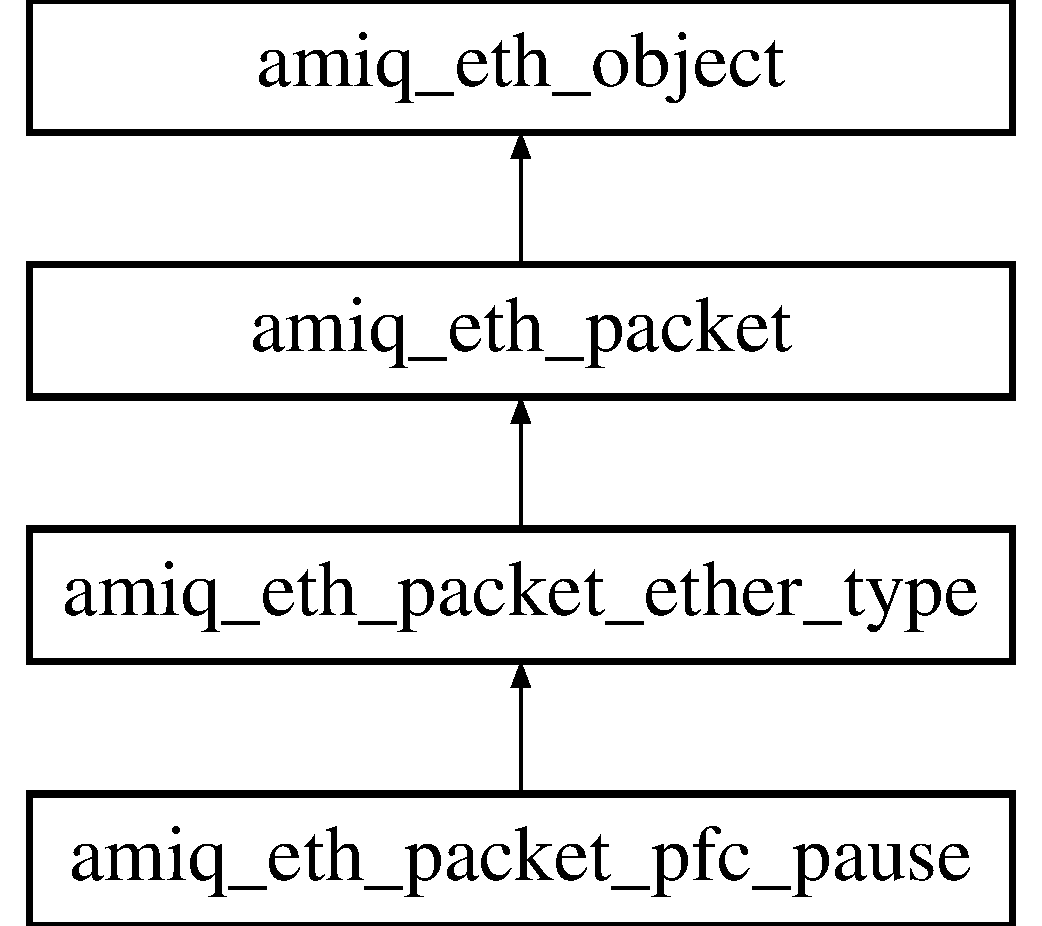
\includegraphics[height=4cm]{classamiq__eth__packet__pfc__pause}
\end{center}
\end{figure}
\subsection*{Public Member Functions}
\begin{DoxyCompactItemize}
\item 
\hyperlink{classamiq__eth__packet__pfc__pause_a28632a96a7692e0c6671be8e6f274b38}{amiq\_\-eth\_\-packet\_\-pfc\_\-pause} ()
\item 
virtual \hyperlink{classamiq__eth__packet__pfc__pause_ac065ae8ab2a4be786b1aee99ebfc8aeb}{$\sim$amiq\_\-eth\_\-packet\_\-pfc\_\-pause} ()
\item 
virtual void \hyperlink{classamiq__eth__packet__pfc__pause_a58c67ea445a72bc6c1c584625d642899}{do\_\-print} (ostream \&out) const 
\item 
virtual void \hyperlink{classamiq__eth__packet__pfc__pause_ac06dfc3d16b73113bbd42460ddbc9c4b}{do\_\-pack} (\hyperlink{classamiq__eth__packer}{amiq\_\-eth\_\-packer} \&packer) const 
\item 
virtual void \hyperlink{classamiq__eth__packet__pfc__pause_abc86009030a38ab03469c697ffec73f6}{do\_\-unpack} (\hyperlink{classamiq__eth__packer}{amiq\_\-eth\_\-packer} \&packer)
\item 
virtual tlm\_\-generic\_\-payload $\ast$ \hyperlink{classamiq__eth__packet__pfc__pause_aaf46b734371ab160eba8764a4e398516}{to\_\-generic\_\-payload} () const 
\end{DoxyCompactItemize}
\subsection*{Public Attributes}
\begin{DoxyCompactItemize}
\item 
\hyperlink{amiq__eth__types_8cpp_a882c4ca2cfd45ca7e4ab471fbaf6f348}{amiq\_\-eth\_\-pause\_\-opcode} \hyperlink{classamiq__eth__packet__pfc__pause_a3248fdfd92b4e26b170f0bd2d0d26229}{pfc\_\-opcode}
\item 
\hyperlink{amiq__eth__types_8cpp_acc82296c2a916d6803e1dd4db06b8a92}{amiq\_\-eth\_\-pfc\_\-class\_\-enable\_\-vector} \hyperlink{classamiq__eth__packet__pfc__pause_a9f34f218b2b2fdb3f9459277a465f220}{pfc\_\-class\_\-enable\_\-vector}
\item 
\hyperlink{amiq__eth__types_8cpp_a9506f5917bf0b1e03bd6946e62cc4a55}{amiq\_\-eth\_\-pause\_\-parameter} $\ast$ \hyperlink{classamiq__eth__packet__pfc__pause_a3cb76fb31642258056bfb06d8844b0cf}{pfc\_\-parameter}
\item 
\hyperlink{amiq__eth__types_8cpp_a3595a0a508d433d383d3e5521fc0b723}{amiq\_\-eth\_\-data} $\ast$ \hyperlink{classamiq__eth__packet__pfc__pause_a70fc4ed398159e0af2d8fc40f0476ed3}{pad}
\item 
\hyperlink{amiq__eth__types_8cpp_adb511dc715b55539c6abdad1de981a9f}{amiq\_\-eth\_\-fcs} \hyperlink{classamiq__eth__packet__pfc__pause_a5cc679d0d63288a1494f7e5bc6316012}{fcs}
\item 
unsigned int \hyperlink{classamiq__eth__packet__pfc__pause_af7531f2b33d11bf9b841357d611bfd8f}{pfc\_\-parameter\_\-size}
\item 
unsigned int \hyperlink{classamiq__eth__packet__pfc__pause_a74ea8b2618525e64c9cad21dc4927f6b}{pad\_\-size}
\item 
bool \hyperlink{classamiq__eth__packet__pfc__pause_a83a474ef0ddf54b1a5d67d4ec155fb37}{print\_\-lists}
\end{DoxyCompactItemize}


\subsection{Detailed Description}


Definition at line 30 of file amiq\_\-eth\_\-packet\_\-pfc\_\-pause.cpp.

\subsection{Constructor \& Destructor Documentation}
\hypertarget{classamiq__eth__packet__pfc__pause_a28632a96a7692e0c6671be8e6f274b38}{
\index{amiq\_\-eth\_\-packet\_\-pfc\_\-pause@{amiq\_\-eth\_\-packet\_\-pfc\_\-pause}!amiq\_\-eth\_\-packet\_\-pfc\_\-pause@{amiq\_\-eth\_\-packet\_\-pfc\_\-pause}}
\index{amiq\_\-eth\_\-packet\_\-pfc\_\-pause@{amiq\_\-eth\_\-packet\_\-pfc\_\-pause}!amiq_eth_packet_pfc_pause@{amiq\_\-eth\_\-packet\_\-pfc\_\-pause}}
\subsubsection[{amiq\_\-eth\_\-packet\_\-pfc\_\-pause}]{\setlength{\rightskip}{0pt plus 5cm}amiq\_\-eth\_\-packet\_\-pfc\_\-pause::amiq\_\-eth\_\-packet\_\-pfc\_\-pause ()\hspace{0.3cm}{\ttfamily  \mbox{[}inline\mbox{]}}}}
\label{classamiq__eth__packet__pfc__pause_a28632a96a7692e0c6671be8e6f274b38}


Definition at line 57 of file amiq\_\-eth\_\-packet\_\-pfc\_\-pause.cpp.

References AMIQ\_\-ETH\_\-DATA\_\-WIDTH, AMIQ\_\-ETH\_\-PAYLOAD\_\-SIZE\_\-MIN, AMIQ\_\-ETH\_\-PFC\_\-CLASS\_\-ENABLE\_\-VECTOR\_\-WIDTH, AMIQ\_\-ETH\_\-PFC\_\-NUMBER\_\-OF\_\-PARAMETERS, AMIQ\_\-ETH\_\-PFC\_\-OPCODE, AMIQ\_\-ETH\_\-PFC\_\-OPCODE\_\-WIDTH, AMIQ\_\-ETH\_\-PFC\_\-PACKET\_\-DESTINATION\_\-ADDRESS, AMIQ\_\-ETH\_\-PFC\_\-PARAMETER\_\-WIDTH, amiq\_\-eth\_\-packet::destination\_\-address, amiq\_\-eth\_\-packet\_\-ether\_\-type::ether\_\-type, NULL, pad, pad\_\-size, pfc\_\-opcode, pfc\_\-parameter, pfc\_\-parameter\_\-size, print\_\-lists, and SC\_\-AMIQ\_\-ETH\_\-MAC\_\-CONTROL.\hypertarget{classamiq__eth__packet__pfc__pause_ac065ae8ab2a4be786b1aee99ebfc8aeb}{
\index{amiq\_\-eth\_\-packet\_\-pfc\_\-pause@{amiq\_\-eth\_\-packet\_\-pfc\_\-pause}!$\sim$amiq\_\-eth\_\-packet\_\-pfc\_\-pause@{$\sim$amiq\_\-eth\_\-packet\_\-pfc\_\-pause}}
\index{$\sim$amiq\_\-eth\_\-packet\_\-pfc\_\-pause@{$\sim$amiq\_\-eth\_\-packet\_\-pfc\_\-pause}!amiq_eth_packet_pfc_pause@{amiq\_\-eth\_\-packet\_\-pfc\_\-pause}}
\subsubsection[{$\sim$amiq\_\-eth\_\-packet\_\-pfc\_\-pause}]{\setlength{\rightskip}{0pt plus 5cm}virtual amiq\_\-eth\_\-packet\_\-pfc\_\-pause::$\sim$amiq\_\-eth\_\-packet\_\-pfc\_\-pause ()\hspace{0.3cm}{\ttfamily  \mbox{[}inline, virtual\mbox{]}}}}
\label{classamiq__eth__packet__pfc__pause_ac065ae8ab2a4be786b1aee99ebfc8aeb}


Definition at line 74 of file amiq\_\-eth\_\-packet\_\-pfc\_\-pause.cpp.

\subsection{Member Function Documentation}
\hypertarget{classamiq__eth__packet__pfc__pause_ac06dfc3d16b73113bbd42460ddbc9c4b}{
\index{amiq\_\-eth\_\-packet\_\-pfc\_\-pause@{amiq\_\-eth\_\-packet\_\-pfc\_\-pause}!do\_\-pack@{do\_\-pack}}
\index{do\_\-pack@{do\_\-pack}!amiq_eth_packet_pfc_pause@{amiq\_\-eth\_\-packet\_\-pfc\_\-pause}}
\subsubsection[{do\_\-pack}]{\setlength{\rightskip}{0pt plus 5cm}virtual void amiq\_\-eth\_\-packet\_\-pfc\_\-pause::do\_\-pack ({\bf amiq\_\-eth\_\-packer} \& {\em packer}) const\hspace{0.3cm}{\ttfamily  \mbox{[}inline, virtual\mbox{]}}}}
\label{classamiq__eth__packet__pfc__pause_ac06dfc3d16b73113bbd42460ddbc9c4b}


Reimplemented from \hyperlink{classamiq__eth__packet__ether__type_a62fe5f26a466f0bd0045599b89aa6926}{amiq\_\-eth\_\-packet\_\-ether\_\-type}.

Definition at line 96 of file amiq\_\-eth\_\-packet\_\-pfc\_\-pause.cpp.

References amiq\_\-eth\_\-do\_\-pack(), fcs, pad, pad\_\-size, pfc\_\-class\_\-enable\_\-vector, pfc\_\-opcode, pfc\_\-parameter, and pfc\_\-parameter\_\-size.\hypertarget{classamiq__eth__packet__pfc__pause_a58c67ea445a72bc6c1c584625d642899}{
\index{amiq\_\-eth\_\-packet\_\-pfc\_\-pause@{amiq\_\-eth\_\-packet\_\-pfc\_\-pause}!do\_\-print@{do\_\-print}}
\index{do\_\-print@{do\_\-print}!amiq_eth_packet_pfc_pause@{amiq\_\-eth\_\-packet\_\-pfc\_\-pause}}
\subsubsection[{do\_\-print}]{\setlength{\rightskip}{0pt plus 5cm}virtual void amiq\_\-eth\_\-packet\_\-pfc\_\-pause::do\_\-print (ostream \& {\em out}) const\hspace{0.3cm}{\ttfamily  \mbox{[}inline, virtual\mbox{]}}}}
\label{classamiq__eth__packet__pfc__pause_a58c67ea445a72bc6c1c584625d642899}


Reimplemented from \hyperlink{classamiq__eth__packet__ether__type_a9b2852fa1aaf278138fde2232e446f63}{amiq\_\-eth\_\-packet\_\-ether\_\-type}.

Definition at line 79 of file amiq\_\-eth\_\-packet\_\-pfc\_\-pause.cpp.

References AMIQ\_\-ETH\_\-FIELD\_\-SEPARATOR, fcs, pad\_\-size, pfc\_\-class\_\-enable\_\-vector, pfc\_\-opcode, pfc\_\-parameter, pfc\_\-parameter\_\-size, and print\_\-lists.\hypertarget{classamiq__eth__packet__pfc__pause_abc86009030a38ab03469c697ffec73f6}{
\index{amiq\_\-eth\_\-packet\_\-pfc\_\-pause@{amiq\_\-eth\_\-packet\_\-pfc\_\-pause}!do\_\-unpack@{do\_\-unpack}}
\index{do\_\-unpack@{do\_\-unpack}!amiq_eth_packet_pfc_pause@{amiq\_\-eth\_\-packet\_\-pfc\_\-pause}}
\subsubsection[{do\_\-unpack}]{\setlength{\rightskip}{0pt plus 5cm}virtual void amiq\_\-eth\_\-packet\_\-pfc\_\-pause::do\_\-unpack ({\bf amiq\_\-eth\_\-packer} \& {\em packer})\hspace{0.3cm}{\ttfamily  \mbox{[}inline, virtual\mbox{]}}}}
\label{classamiq__eth__packet__pfc__pause_abc86009030a38ab03469c697ffec73f6}


Reimplemented from \hyperlink{classamiq__eth__packet__ether__type_a0c86ef80c46bbed384739b23e5efb0ef}{amiq\_\-eth\_\-packet\_\-ether\_\-type}.

Definition at line 116 of file amiq\_\-eth\_\-packet\_\-pfc\_\-pause.cpp.

References amiq\_\-eth\_\-do\_\-unpack(), fcs, pad, pad\_\-size, pfc\_\-class\_\-enable\_\-vector, pfc\_\-opcode, pfc\_\-parameter, and pfc\_\-parameter\_\-size.\hypertarget{classamiq__eth__packet__pfc__pause_aaf46b734371ab160eba8764a4e398516}{
\index{amiq\_\-eth\_\-packet\_\-pfc\_\-pause@{amiq\_\-eth\_\-packet\_\-pfc\_\-pause}!to\_\-generic\_\-payload@{to\_\-generic\_\-payload}}
\index{to\_\-generic\_\-payload@{to\_\-generic\_\-payload}!amiq_eth_packet_pfc_pause@{amiq\_\-eth\_\-packet\_\-pfc\_\-pause}}
\subsubsection[{to\_\-generic\_\-payload}]{\setlength{\rightskip}{0pt plus 5cm}virtual tlm\_\-generic\_\-payload$\ast$ amiq\_\-eth\_\-packet\_\-pfc\_\-pause::to\_\-generic\_\-payload () const\hspace{0.3cm}{\ttfamily  \mbox{[}inline, virtual\mbox{]}}}}
\label{classamiq__eth__packet__pfc__pause_aaf46b734371ab160eba8764a4e398516}


Reimplemented from \hyperlink{classamiq__eth__packet_a6dd92751d8172eeaa347d71bb415b0d5}{amiq\_\-eth\_\-packet}.

Definition at line 140 of file amiq\_\-eth\_\-packet\_\-pfc\_\-pause.cpp.

References AMIQ\_\-ETH\_\-PACKET\_\-PFC\_\-PAUSE\_\-CODE.

\subsection{Member Data Documentation}
\hypertarget{classamiq__eth__packet__pfc__pause_a5cc679d0d63288a1494f7e5bc6316012}{
\index{amiq\_\-eth\_\-packet\_\-pfc\_\-pause@{amiq\_\-eth\_\-packet\_\-pfc\_\-pause}!fcs@{fcs}}
\index{fcs@{fcs}!amiq_eth_packet_pfc_pause@{amiq\_\-eth\_\-packet\_\-pfc\_\-pause}}
\subsubsection[{fcs}]{\setlength{\rightskip}{0pt plus 5cm}{\bf amiq\_\-eth\_\-fcs} {\bf amiq\_\-eth\_\-packet\_\-pfc\_\-pause::fcs}}}
\label{classamiq__eth__packet__pfc__pause_a5cc679d0d63288a1494f7e5bc6316012}


Definition at line 47 of file amiq\_\-eth\_\-packet\_\-pfc\_\-pause.cpp.

Referenced by do\_\-pack(), do\_\-print(), and do\_\-unpack().\hypertarget{classamiq__eth__packet__pfc__pause_a70fc4ed398159e0af2d8fc40f0476ed3}{
\index{amiq\_\-eth\_\-packet\_\-pfc\_\-pause@{amiq\_\-eth\_\-packet\_\-pfc\_\-pause}!pad@{pad}}
\index{pad@{pad}!amiq_eth_packet_pfc_pause@{amiq\_\-eth\_\-packet\_\-pfc\_\-pause}}
\subsubsection[{pad}]{\setlength{\rightskip}{0pt plus 5cm}{\bf amiq\_\-eth\_\-data}$\ast$ {\bf amiq\_\-eth\_\-packet\_\-pfc\_\-pause::pad}}}
\label{classamiq__eth__packet__pfc__pause_a70fc4ed398159e0af2d8fc40f0476ed3}


Definition at line 44 of file amiq\_\-eth\_\-packet\_\-pfc\_\-pause.cpp.

Referenced by amiq\_\-eth\_\-packet\_\-pfc\_\-pause(), do\_\-pack(), and do\_\-unpack().\hypertarget{classamiq__eth__packet__pfc__pause_a74ea8b2618525e64c9cad21dc4927f6b}{
\index{amiq\_\-eth\_\-packet\_\-pfc\_\-pause@{amiq\_\-eth\_\-packet\_\-pfc\_\-pause}!pad\_\-size@{pad\_\-size}}
\index{pad\_\-size@{pad\_\-size}!amiq_eth_packet_pfc_pause@{amiq\_\-eth\_\-packet\_\-pfc\_\-pause}}
\subsubsection[{pad\_\-size}]{\setlength{\rightskip}{0pt plus 5cm}unsigned int {\bf amiq\_\-eth\_\-packet\_\-pfc\_\-pause::pad\_\-size}}}
\label{classamiq__eth__packet__pfc__pause_a74ea8b2618525e64c9cad21dc4927f6b}


Definition at line 51 of file amiq\_\-eth\_\-packet\_\-pfc\_\-pause.cpp.

Referenced by amiq\_\-eth\_\-packet\_\-pfc\_\-pause(), do\_\-pack(), do\_\-print(), and do\_\-unpack().\hypertarget{classamiq__eth__packet__pfc__pause_a9f34f218b2b2fdb3f9459277a465f220}{
\index{amiq\_\-eth\_\-packet\_\-pfc\_\-pause@{amiq\_\-eth\_\-packet\_\-pfc\_\-pause}!pfc\_\-class\_\-enable\_\-vector@{pfc\_\-class\_\-enable\_\-vector}}
\index{pfc\_\-class\_\-enable\_\-vector@{pfc\_\-class\_\-enable\_\-vector}!amiq_eth_packet_pfc_pause@{amiq\_\-eth\_\-packet\_\-pfc\_\-pause}}
\subsubsection[{pfc\_\-class\_\-enable\_\-vector}]{\setlength{\rightskip}{0pt plus 5cm}{\bf amiq\_\-eth\_\-pfc\_\-class\_\-enable\_\-vector} {\bf amiq\_\-eth\_\-packet\_\-pfc\_\-pause::pfc\_\-class\_\-enable\_\-vector}}}
\label{classamiq__eth__packet__pfc__pause_a9f34f218b2b2fdb3f9459277a465f220}


Definition at line 38 of file amiq\_\-eth\_\-packet\_\-pfc\_\-pause.cpp.

Referenced by do\_\-pack(), do\_\-print(), and do\_\-unpack().\hypertarget{classamiq__eth__packet__pfc__pause_a3248fdfd92b4e26b170f0bd2d0d26229}{
\index{amiq\_\-eth\_\-packet\_\-pfc\_\-pause@{amiq\_\-eth\_\-packet\_\-pfc\_\-pause}!pfc\_\-opcode@{pfc\_\-opcode}}
\index{pfc\_\-opcode@{pfc\_\-opcode}!amiq_eth_packet_pfc_pause@{amiq\_\-eth\_\-packet\_\-pfc\_\-pause}}
\subsubsection[{pfc\_\-opcode}]{\setlength{\rightskip}{0pt plus 5cm}{\bf amiq\_\-eth\_\-pause\_\-opcode} {\bf amiq\_\-eth\_\-packet\_\-pfc\_\-pause::pfc\_\-opcode}}}
\label{classamiq__eth__packet__pfc__pause_a3248fdfd92b4e26b170f0bd2d0d26229}


Definition at line 35 of file amiq\_\-eth\_\-packet\_\-pfc\_\-pause.cpp.

Referenced by amiq\_\-eth\_\-packet\_\-pfc\_\-pause(), do\_\-pack(), do\_\-print(), and do\_\-unpack().\hypertarget{classamiq__eth__packet__pfc__pause_a3cb76fb31642258056bfb06d8844b0cf}{
\index{amiq\_\-eth\_\-packet\_\-pfc\_\-pause@{amiq\_\-eth\_\-packet\_\-pfc\_\-pause}!pfc\_\-parameter@{pfc\_\-parameter}}
\index{pfc\_\-parameter@{pfc\_\-parameter}!amiq_eth_packet_pfc_pause@{amiq\_\-eth\_\-packet\_\-pfc\_\-pause}}
\subsubsection[{pfc\_\-parameter}]{\setlength{\rightskip}{0pt plus 5cm}{\bf amiq\_\-eth\_\-pause\_\-parameter}$\ast$ {\bf amiq\_\-eth\_\-packet\_\-pfc\_\-pause::pfc\_\-parameter}}}
\label{classamiq__eth__packet__pfc__pause_a3cb76fb31642258056bfb06d8844b0cf}


Definition at line 41 of file amiq\_\-eth\_\-packet\_\-pfc\_\-pause.cpp.

Referenced by amiq\_\-eth\_\-packet\_\-pfc\_\-pause(), do\_\-pack(), do\_\-print(), and do\_\-unpack().\hypertarget{classamiq__eth__packet__pfc__pause_af7531f2b33d11bf9b841357d611bfd8f}{
\index{amiq\_\-eth\_\-packet\_\-pfc\_\-pause@{amiq\_\-eth\_\-packet\_\-pfc\_\-pause}!pfc\_\-parameter\_\-size@{pfc\_\-parameter\_\-size}}
\index{pfc\_\-parameter\_\-size@{pfc\_\-parameter\_\-size}!amiq_eth_packet_pfc_pause@{amiq\_\-eth\_\-packet\_\-pfc\_\-pause}}
\subsubsection[{pfc\_\-parameter\_\-size}]{\setlength{\rightskip}{0pt plus 5cm}unsigned int {\bf amiq\_\-eth\_\-packet\_\-pfc\_\-pause::pfc\_\-parameter\_\-size}}}
\label{classamiq__eth__packet__pfc__pause_af7531f2b33d11bf9b841357d611bfd8f}


Definition at line 49 of file amiq\_\-eth\_\-packet\_\-pfc\_\-pause.cpp.

Referenced by amiq\_\-eth\_\-packet\_\-pfc\_\-pause(), do\_\-pack(), do\_\-print(), and do\_\-unpack().\hypertarget{classamiq__eth__packet__pfc__pause_a83a474ef0ddf54b1a5d67d4ec155fb37}{
\index{amiq\_\-eth\_\-packet\_\-pfc\_\-pause@{amiq\_\-eth\_\-packet\_\-pfc\_\-pause}!print\_\-lists@{print\_\-lists}}
\index{print\_\-lists@{print\_\-lists}!amiq_eth_packet_pfc_pause@{amiq\_\-eth\_\-packet\_\-pfc\_\-pause}}
\subsubsection[{print\_\-lists}]{\setlength{\rightskip}{0pt plus 5cm}bool {\bf amiq\_\-eth\_\-packet\_\-pfc\_\-pause::print\_\-lists}}}
\label{classamiq__eth__packet__pfc__pause_a83a474ef0ddf54b1a5d67d4ec155fb37}


Definition at line 54 of file amiq\_\-eth\_\-packet\_\-pfc\_\-pause.cpp.

Referenced by amiq\_\-eth\_\-packet\_\-pfc\_\-pause(), and do\_\-print().

The documentation for this class was generated from the following file:\begin{DoxyCompactItemize}
\item 
/home/cristian.slav/work/amiq/projects/sv/amiq\_\-eth/sc/\hyperlink{amiq__eth__packet__pfc__pause_8cpp}{amiq\_\-eth\_\-packet\_\-pfc\_\-pause.cpp}\end{DoxyCompactItemize}

\hypertarget{classamiq__eth__packet__ptp}{
\section{amiq\_\-eth\_\-packet\_\-ptp Class Reference}
\label{classamiq__eth__packet__ptp}\index{amiq\_\-eth\_\-packet\_\-ptp@{amiq\_\-eth\_\-packet\_\-ptp}}
}
Inheritance diagram for amiq\_\-eth\_\-packet\_\-ptp::\begin{figure}[H]
\begin{center}
\leavevmode
\includegraphics[height=4cm]{classamiq__eth__packet__ptp}
\end{center}
\end{figure}
\subsection*{Public Member Functions}
\begin{DoxyCompactItemize}
\item 
\hyperlink{classamiq__eth__packet__ptp_a20167ddce08cead24360e27ac9e1e570}{amiq\_\-eth\_\-packet\_\-ptp} ()
\item 
virtual \hyperlink{classamiq__eth__packet__ptp_a3970961ac5aec4bb174e10bc463117bb}{$\sim$amiq\_\-eth\_\-packet\_\-ptp} ()
\item 
virtual void \hyperlink{classamiq__eth__packet__ptp_ab7bc36daf8f06a4c65e4cbe4c84a04a7}{pack\_\-fcs} (\hyperlink{classamiq__eth__packer}{amiq\_\-eth\_\-packer} \&packer) const 
\item 
virtual void \hyperlink{classamiq__eth__packet__ptp_aa9c14abac259c28ca17c69eecaa5a403}{pack\_\-body} (\hyperlink{classamiq__eth__packer}{amiq\_\-eth\_\-packer} \&packer) const 
\item 
virtual void \hyperlink{classamiq__eth__packet__ptp_a5d415af5fcb6ed2cb603aaf0105fdd43}{do\_\-pack} (\hyperlink{classamiq__eth__packer}{amiq\_\-eth\_\-packer} \&packer) const 
\item 
virtual void \hyperlink{classamiq__eth__packet__ptp_a831addd66dff7e42f2e2e9edb6f976b3}{do\_\-unpack} (\hyperlink{classamiq__eth__packer}{amiq\_\-eth\_\-packer} \&packer)
\item 
virtual void \hyperlink{classamiq__eth__packet__ptp_a68337ad7c7971f267b692dfbd92ede7b}{do\_\-pack\_\-for\_\-fcs} (\hyperlink{classamiq__eth__packer}{amiq\_\-eth\_\-packer} \&packer) const 
\item 
virtual void \hyperlink{classamiq__eth__packet__ptp_a52db9ab62ab743317a7ca4745a823a82}{do\_\-print} (ostream \&out) const 
\item 
virtual tlm\_\-generic\_\-payload $\ast$ \hyperlink{classamiq__eth__packet__ptp_a7c1a6b1207ce7e9e604e05cd883bccc0}{to\_\-generic\_\-payload} () const 
\end{DoxyCompactItemize}
\subsection*{Public Attributes}
\begin{DoxyCompactItemize}
\item 
\hyperlink{classamiq__eth__packet__ptp__header}{amiq\_\-eth\_\-packet\_\-ptp\_\-header} \hyperlink{classamiq__eth__packet__ptp_a09df382a165bd23e508f402ff0833c36}{header}
\item 
\hyperlink{classamiq__eth__packet__ptp__announce__message}{amiq\_\-eth\_\-packet\_\-ptp\_\-announce\_\-message} \hyperlink{classamiq__eth__packet__ptp_a6d3636995bf83da8721a245b27495e24}{announce\_\-message\_\-body}
\item 
\hyperlink{classamiq__eth__packet__ptp__sync__message}{amiq\_\-eth\_\-packet\_\-ptp\_\-sync\_\-message} \hyperlink{classamiq__eth__packet__ptp_ad28ea57af5d6111b1724fb14e995d30c}{sync\_\-message\_\-body}
\item 
\hyperlink{classamiq__eth__packet__ptp__delay__req__message}{amiq\_\-eth\_\-packet\_\-ptp\_\-delay\_\-req\_\-message} \hyperlink{classamiq__eth__packet__ptp_ad1117b52c9080df91e256d2649281547}{delay\_\-req\_\-message\_\-body}
\item 
\hyperlink{amiq__eth__types_8cpp_adb511dc715b55539c6abdad1de981a9f}{amiq\_\-eth\_\-fcs} \hyperlink{classamiq__eth__packet__ptp_a05a43b6fa83d4473878a59b44b8be088}{fcs}
\end{DoxyCompactItemize}


\subsection{Detailed Description}


Definition at line 469 of file amiq\_\-eth\_\-packet\_\-ptp.cpp.

\subsection{Constructor \& Destructor Documentation}
\hypertarget{classamiq__eth__packet__ptp_a20167ddce08cead24360e27ac9e1e570}{
\index{amiq\_\-eth\_\-packet\_\-ptp@{amiq\_\-eth\_\-packet\_\-ptp}!amiq\_\-eth\_\-packet\_\-ptp@{amiq\_\-eth\_\-packet\_\-ptp}}
\index{amiq\_\-eth\_\-packet\_\-ptp@{amiq\_\-eth\_\-packet\_\-ptp}!amiq_eth_packet_ptp@{amiq\_\-eth\_\-packet\_\-ptp}}
\subsubsection[{amiq\_\-eth\_\-packet\_\-ptp}]{\setlength{\rightskip}{0pt plus 5cm}amiq\_\-eth\_\-packet\_\-ptp::amiq\_\-eth\_\-packet\_\-ptp ()\hspace{0.3cm}{\ttfamily  \mbox{[}inline\mbox{]}}}}
\label{classamiq__eth__packet__ptp_a20167ddce08cead24360e27ac9e1e570}


Definition at line 485 of file amiq\_\-eth\_\-packet\_\-ptp.cpp.

References delay\_\-req\_\-message\_\-body, amiq\_\-eth\_\-packet\_\-ether\_\-type::ether\_\-type, header, SC\_\-AMIQ\_\-ETH\_\-PTP, and sync\_\-message\_\-body.\hypertarget{classamiq__eth__packet__ptp_a3970961ac5aec4bb174e10bc463117bb}{
\index{amiq\_\-eth\_\-packet\_\-ptp@{amiq\_\-eth\_\-packet\_\-ptp}!$\sim$amiq\_\-eth\_\-packet\_\-ptp@{$\sim$amiq\_\-eth\_\-packet\_\-ptp}}
\index{$\sim$amiq\_\-eth\_\-packet\_\-ptp@{$\sim$amiq\_\-eth\_\-packet\_\-ptp}!amiq_eth_packet_ptp@{amiq\_\-eth\_\-packet\_\-ptp}}
\subsubsection[{$\sim$amiq\_\-eth\_\-packet\_\-ptp}]{\setlength{\rightskip}{0pt plus 5cm}virtual amiq\_\-eth\_\-packet\_\-ptp::$\sim$amiq\_\-eth\_\-packet\_\-ptp ()\hspace{0.3cm}{\ttfamily  \mbox{[}inline, virtual\mbox{]}}}}
\label{classamiq__eth__packet__ptp_a3970961ac5aec4bb174e10bc463117bb}


Definition at line 493 of file amiq\_\-eth\_\-packet\_\-ptp.cpp.

References delay\_\-req\_\-message\_\-body, header, and sync\_\-message\_\-body.

\subsection{Member Function Documentation}
\hypertarget{classamiq__eth__packet__ptp_a5d415af5fcb6ed2cb603aaf0105fdd43}{
\index{amiq\_\-eth\_\-packet\_\-ptp@{amiq\_\-eth\_\-packet\_\-ptp}!do\_\-pack@{do\_\-pack}}
\index{do\_\-pack@{do\_\-pack}!amiq_eth_packet_ptp@{amiq\_\-eth\_\-packet\_\-ptp}}
\subsubsection[{do\_\-pack}]{\setlength{\rightskip}{0pt plus 5cm}virtual void amiq\_\-eth\_\-packet\_\-ptp::do\_\-pack ({\bf amiq\_\-eth\_\-packer} \& {\em packer}) const\hspace{0.3cm}{\ttfamily  \mbox{[}inline, virtual\mbox{]}}}}
\label{classamiq__eth__packet__ptp_a5d415af5fcb6ed2cb603aaf0105fdd43}


Reimplemented from \hyperlink{classamiq__eth__packet__ether__type_a62fe5f26a466f0bd0045599b89aa6926}{amiq\_\-eth\_\-packet\_\-ether\_\-type}.

Definition at line 529 of file amiq\_\-eth\_\-packet\_\-ptp.cpp.

References amiq\_\-eth\_\-packet\_\-ptp\_\-header::do\_\-pack(), header, pack\_\-body(), and pack\_\-fcs().\hypertarget{classamiq__eth__packet__ptp_a68337ad7c7971f267b692dfbd92ede7b}{
\index{amiq\_\-eth\_\-packet\_\-ptp@{amiq\_\-eth\_\-packet\_\-ptp}!do\_\-pack\_\-for\_\-fcs@{do\_\-pack\_\-for\_\-fcs}}
\index{do\_\-pack\_\-for\_\-fcs@{do\_\-pack\_\-for\_\-fcs}!amiq_eth_packet_ptp@{amiq\_\-eth\_\-packet\_\-ptp}}
\subsubsection[{do\_\-pack\_\-for\_\-fcs}]{\setlength{\rightskip}{0pt plus 5cm}virtual void amiq\_\-eth\_\-packet\_\-ptp::do\_\-pack\_\-for\_\-fcs ({\bf amiq\_\-eth\_\-packer} \& {\em packer}) const\hspace{0.3cm}{\ttfamily  \mbox{[}inline, virtual\mbox{]}}}}
\label{classamiq__eth__packet__ptp_a68337ad7c7971f267b692dfbd92ede7b}


Reimplemented from \hyperlink{classamiq__eth__packet__ether__type_aaa85cf778650e1c1b377392a975cb7bc}{amiq\_\-eth\_\-packet\_\-ether\_\-type}.

Definition at line 565 of file amiq\_\-eth\_\-packet\_\-ptp.cpp.

References amiq\_\-eth\_\-packet\_\-ptp\_\-header::do\_\-pack(), header, and pack\_\-body().\hypertarget{classamiq__eth__packet__ptp_a52db9ab62ab743317a7ca4745a823a82}{
\index{amiq\_\-eth\_\-packet\_\-ptp@{amiq\_\-eth\_\-packet\_\-ptp}!do\_\-print@{do\_\-print}}
\index{do\_\-print@{do\_\-print}!amiq_eth_packet_ptp@{amiq\_\-eth\_\-packet\_\-ptp}}
\subsubsection[{do\_\-print}]{\setlength{\rightskip}{0pt plus 5cm}virtual void amiq\_\-eth\_\-packet\_\-ptp::do\_\-print (ostream \& {\em out}) const\hspace{0.3cm}{\ttfamily  \mbox{[}inline, virtual\mbox{]}}}}
\label{classamiq__eth__packet__ptp_a52db9ab62ab743317a7ca4745a823a82}


Reimplemented from \hyperlink{classamiq__eth__packet__ether__type_a9b2852fa1aaf278138fde2232e446f63}{amiq\_\-eth\_\-packet\_\-ether\_\-type}.

Definition at line 573 of file amiq\_\-eth\_\-packet\_\-ptp.cpp.

References AMIQ\_\-ETH\_\-FIELD\_\-SEPARATOR, announce\_\-message\_\-body, delay\_\-req\_\-message\_\-body, amiq\_\-eth\_\-packet\_\-ptp\_\-delay\_\-req\_\-message::do\_\-print(), amiq\_\-eth\_\-packet\_\-ptp\_\-sync\_\-message::do\_\-print(), amiq\_\-eth\_\-packet\_\-ptp\_\-announce\_\-message::do\_\-print(), amiq\_\-eth\_\-packet\_\-ptp\_\-header::do\_\-print(), fcs, amiq\_\-eth\_\-packet::get\_\-correct\_\-fcs(), header, amiq\_\-eth\_\-packet\_\-ptp\_\-header::message\_\-type, PTP\_\-AnnounceMessage, PTP\_\-Delay\_\-ReqMessage, PTP\_\-SyncMessage, and sync\_\-message\_\-body.\hypertarget{classamiq__eth__packet__ptp_a831addd66dff7e42f2e2e9edb6f976b3}{
\index{amiq\_\-eth\_\-packet\_\-ptp@{amiq\_\-eth\_\-packet\_\-ptp}!do\_\-unpack@{do\_\-unpack}}
\index{do\_\-unpack@{do\_\-unpack}!amiq_eth_packet_ptp@{amiq\_\-eth\_\-packet\_\-ptp}}
\subsubsection[{do\_\-unpack}]{\setlength{\rightskip}{0pt plus 5cm}virtual void amiq\_\-eth\_\-packet\_\-ptp::do\_\-unpack ({\bf amiq\_\-eth\_\-packer} \& {\em packer})\hspace{0.3cm}{\ttfamily  \mbox{[}inline, virtual\mbox{]}}}}
\label{classamiq__eth__packet__ptp_a831addd66dff7e42f2e2e9edb6f976b3}


Reimplemented from \hyperlink{classamiq__eth__packet__ether__type_a0c86ef80c46bbed384739b23e5efb0ef}{amiq\_\-eth\_\-packet\_\-ether\_\-type}.

Definition at line 538 of file amiq\_\-eth\_\-packet\_\-ptp.cpp.

References amiq\_\-eth\_\-do\_\-unpack(), announce\_\-message\_\-body, delay\_\-req\_\-message\_\-body, amiq\_\-eth\_\-packet\_\-ptp\_\-delay\_\-req\_\-message::do\_\-unpack(), amiq\_\-eth\_\-packet\_\-ptp\_\-sync\_\-message::do\_\-unpack(), amiq\_\-eth\_\-packet\_\-ptp\_\-announce\_\-message::do\_\-unpack(), amiq\_\-eth\_\-packet\_\-ptp\_\-header::do\_\-unpack(), fcs, header, amiq\_\-eth\_\-packet\_\-ptp\_\-header::message\_\-type, PTP\_\-AnnounceMessage, PTP\_\-Delay\_\-ReqMessage, PTP\_\-SyncMessage, and sync\_\-message\_\-body.\hypertarget{classamiq__eth__packet__ptp_aa9c14abac259c28ca17c69eecaa5a403}{
\index{amiq\_\-eth\_\-packet\_\-ptp@{amiq\_\-eth\_\-packet\_\-ptp}!pack\_\-body@{pack\_\-body}}
\index{pack\_\-body@{pack\_\-body}!amiq_eth_packet_ptp@{amiq\_\-eth\_\-packet\_\-ptp}}
\subsubsection[{pack\_\-body}]{\setlength{\rightskip}{0pt plus 5cm}virtual void amiq\_\-eth\_\-packet\_\-ptp::pack\_\-body ({\bf amiq\_\-eth\_\-packer} \& {\em packer}) const\hspace{0.3cm}{\ttfamily  \mbox{[}inline, virtual\mbox{]}}}}
\label{classamiq__eth__packet__ptp_aa9c14abac259c28ca17c69eecaa5a403}


Definition at line 507 of file amiq\_\-eth\_\-packet\_\-ptp.cpp.

References announce\_\-message\_\-body, delay\_\-req\_\-message\_\-body, amiq\_\-eth\_\-packet\_\-ptp\_\-delay\_\-req\_\-message::do\_\-pack(), amiq\_\-eth\_\-packet\_\-ptp\_\-sync\_\-message::do\_\-pack(), amiq\_\-eth\_\-packet\_\-ptp\_\-announce\_\-message::do\_\-pack(), header, amiq\_\-eth\_\-packet\_\-ptp\_\-header::message\_\-type, PTP\_\-AnnounceMessage, PTP\_\-Delay\_\-ReqMessage, PTP\_\-SyncMessage, and sync\_\-message\_\-body.

Referenced by do\_\-pack(), and do\_\-pack\_\-for\_\-fcs().\hypertarget{classamiq__eth__packet__ptp_ab7bc36daf8f06a4c65e4cbe4c84a04a7}{
\index{amiq\_\-eth\_\-packet\_\-ptp@{amiq\_\-eth\_\-packet\_\-ptp}!pack\_\-fcs@{pack\_\-fcs}}
\index{pack\_\-fcs@{pack\_\-fcs}!amiq_eth_packet_ptp@{amiq\_\-eth\_\-packet\_\-ptp}}
\subsubsection[{pack\_\-fcs}]{\setlength{\rightskip}{0pt plus 5cm}virtual void amiq\_\-eth\_\-packet\_\-ptp::pack\_\-fcs ({\bf amiq\_\-eth\_\-packer} \& {\em packer}) const\hspace{0.3cm}{\ttfamily  \mbox{[}inline, virtual\mbox{]}}}}
\label{classamiq__eth__packet__ptp_ab7bc36daf8f06a4c65e4cbe4c84a04a7}


Definition at line 501 of file amiq\_\-eth\_\-packet\_\-ptp.cpp.

References amiq\_\-eth\_\-do\_\-pack(), and fcs.

Referenced by do\_\-pack().\hypertarget{classamiq__eth__packet__ptp_a7c1a6b1207ce7e9e604e05cd883bccc0}{
\index{amiq\_\-eth\_\-packet\_\-ptp@{amiq\_\-eth\_\-packet\_\-ptp}!to\_\-generic\_\-payload@{to\_\-generic\_\-payload}}
\index{to\_\-generic\_\-payload@{to\_\-generic\_\-payload}!amiq_eth_packet_ptp@{amiq\_\-eth\_\-packet\_\-ptp}}
\subsubsection[{to\_\-generic\_\-payload}]{\setlength{\rightskip}{0pt plus 5cm}virtual tlm\_\-generic\_\-payload$\ast$ amiq\_\-eth\_\-packet\_\-ptp::to\_\-generic\_\-payload () const\hspace{0.3cm}{\ttfamily  \mbox{[}inline, virtual\mbox{]}}}}
\label{classamiq__eth__packet__ptp_a7c1a6b1207ce7e9e604e05cd883bccc0}


Reimplemented from \hyperlink{classamiq__eth__packet_a6dd92751d8172eeaa347d71bb415b0d5}{amiq\_\-eth\_\-packet}.

Definition at line 610 of file amiq\_\-eth\_\-packet\_\-ptp.cpp.

References AMIQ\_\-ETH\_\-PACKET\_\-PTP\_\-CODE.

\subsection{Member Data Documentation}
\hypertarget{classamiq__eth__packet__ptp_a6d3636995bf83da8721a245b27495e24}{
\index{amiq\_\-eth\_\-packet\_\-ptp@{amiq\_\-eth\_\-packet\_\-ptp}!announce\_\-message\_\-body@{announce\_\-message\_\-body}}
\index{announce\_\-message\_\-body@{announce\_\-message\_\-body}!amiq_eth_packet_ptp@{amiq\_\-eth\_\-packet\_\-ptp}}
\subsubsection[{announce\_\-message\_\-body}]{\setlength{\rightskip}{0pt plus 5cm}{\bf amiq\_\-eth\_\-packet\_\-ptp\_\-announce\_\-message} {\bf amiq\_\-eth\_\-packet\_\-ptp::announce\_\-message\_\-body}}}
\label{classamiq__eth__packet__ptp_a6d3636995bf83da8721a245b27495e24}


Definition at line 477 of file amiq\_\-eth\_\-packet\_\-ptp.cpp.

Referenced by do\_\-print(), do\_\-unpack(), and pack\_\-body().\hypertarget{classamiq__eth__packet__ptp_ad1117b52c9080df91e256d2649281547}{
\index{amiq\_\-eth\_\-packet\_\-ptp@{amiq\_\-eth\_\-packet\_\-ptp}!delay\_\-req\_\-message\_\-body@{delay\_\-req\_\-message\_\-body}}
\index{delay\_\-req\_\-message\_\-body@{delay\_\-req\_\-message\_\-body}!amiq_eth_packet_ptp@{amiq\_\-eth\_\-packet\_\-ptp}}
\subsubsection[{delay\_\-req\_\-message\_\-body}]{\setlength{\rightskip}{0pt plus 5cm}{\bf amiq\_\-eth\_\-packet\_\-ptp\_\-delay\_\-req\_\-message} {\bf amiq\_\-eth\_\-packet\_\-ptp::delay\_\-req\_\-message\_\-body}}}
\label{classamiq__eth__packet__ptp_ad1117b52c9080df91e256d2649281547}


Definition at line 479 of file amiq\_\-eth\_\-packet\_\-ptp.cpp.

Referenced by amiq\_\-eth\_\-packet\_\-ptp(), do\_\-print(), do\_\-unpack(), pack\_\-body(), and $\sim$amiq\_\-eth\_\-packet\_\-ptp().\hypertarget{classamiq__eth__packet__ptp_a05a43b6fa83d4473878a59b44b8be088}{
\index{amiq\_\-eth\_\-packet\_\-ptp@{amiq\_\-eth\_\-packet\_\-ptp}!fcs@{fcs}}
\index{fcs@{fcs}!amiq_eth_packet_ptp@{amiq\_\-eth\_\-packet\_\-ptp}}
\subsubsection[{fcs}]{\setlength{\rightskip}{0pt plus 5cm}{\bf amiq\_\-eth\_\-fcs} {\bf amiq\_\-eth\_\-packet\_\-ptp::fcs}}}
\label{classamiq__eth__packet__ptp_a05a43b6fa83d4473878a59b44b8be088}


Definition at line 482 of file amiq\_\-eth\_\-packet\_\-ptp.cpp.

Referenced by do\_\-print(), do\_\-unpack(), and pack\_\-fcs().\hypertarget{classamiq__eth__packet__ptp_a09df382a165bd23e508f402ff0833c36}{
\index{amiq\_\-eth\_\-packet\_\-ptp@{amiq\_\-eth\_\-packet\_\-ptp}!header@{header}}
\index{header@{header}!amiq_eth_packet_ptp@{amiq\_\-eth\_\-packet\_\-ptp}}
\subsubsection[{header}]{\setlength{\rightskip}{0pt plus 5cm}{\bf amiq\_\-eth\_\-packet\_\-ptp\_\-header} {\bf amiq\_\-eth\_\-packet\_\-ptp::header}}}
\label{classamiq__eth__packet__ptp_a09df382a165bd23e508f402ff0833c36}


Definition at line 474 of file amiq\_\-eth\_\-packet\_\-ptp.cpp.

Referenced by amiq\_\-eth\_\-packet\_\-ptp(), do\_\-pack(), do\_\-pack\_\-for\_\-fcs(), do\_\-print(), do\_\-unpack(), pack\_\-body(), and $\sim$amiq\_\-eth\_\-packet\_\-ptp().\hypertarget{classamiq__eth__packet__ptp_ad28ea57af5d6111b1724fb14e995d30c}{
\index{amiq\_\-eth\_\-packet\_\-ptp@{amiq\_\-eth\_\-packet\_\-ptp}!sync\_\-message\_\-body@{sync\_\-message\_\-body}}
\index{sync\_\-message\_\-body@{sync\_\-message\_\-body}!amiq_eth_packet_ptp@{amiq\_\-eth\_\-packet\_\-ptp}}
\subsubsection[{sync\_\-message\_\-body}]{\setlength{\rightskip}{0pt plus 5cm}{\bf amiq\_\-eth\_\-packet\_\-ptp\_\-sync\_\-message} {\bf amiq\_\-eth\_\-packet\_\-ptp::sync\_\-message\_\-body}}}
\label{classamiq__eth__packet__ptp_ad28ea57af5d6111b1724fb14e995d30c}


Definition at line 478 of file amiq\_\-eth\_\-packet\_\-ptp.cpp.

Referenced by amiq\_\-eth\_\-packet\_\-ptp(), do\_\-print(), do\_\-unpack(), pack\_\-body(), and $\sim$amiq\_\-eth\_\-packet\_\-ptp().

The documentation for this class was generated from the following file:\begin{DoxyCompactItemize}
\item 
/home/cristian.slav/work/amiq/projects/sv/amiq\_\-eth/sc/\hyperlink{amiq__eth__packet__ptp_8cpp}{amiq\_\-eth\_\-packet\_\-ptp.cpp}\end{DoxyCompactItemize}

\hypertarget{classamiq__eth__packet__ptp__announce__message}{
\section{amiq\_\-eth\_\-packet\_\-ptp\_\-announce\_\-message Class Reference}
\label{classamiq__eth__packet__ptp__announce__message}\index{amiq\_\-eth\_\-packet\_\-ptp\_\-announce\_\-message@{amiq\_\-eth\_\-packet\_\-ptp\_\-announce\_\-message}}
}
Inheritance diagram for amiq\_\-eth\_\-packet\_\-ptp\_\-announce\_\-message::\begin{figure}[H]
\begin{center}
\leavevmode
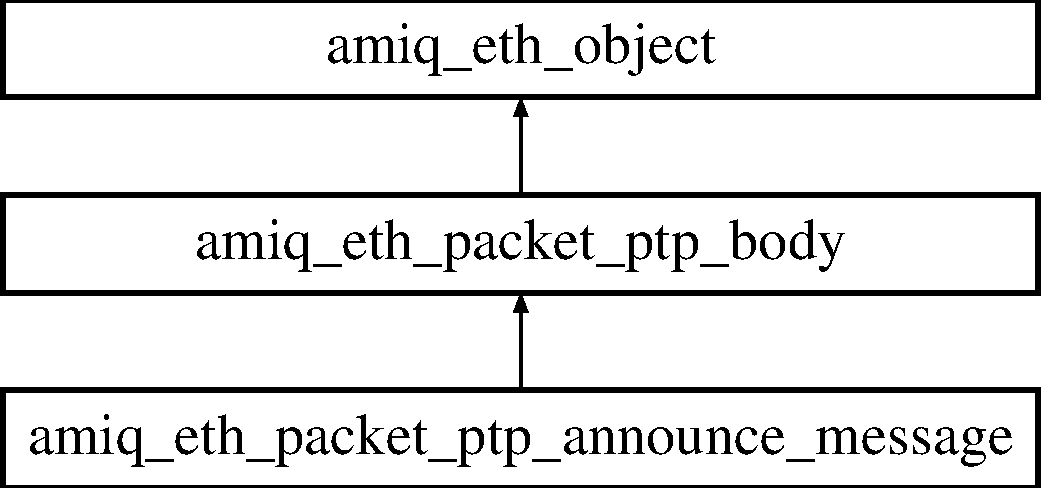
\includegraphics[height=3cm]{classamiq__eth__packet__ptp__announce__message}
\end{center}
\end{figure}
\subsection*{Public Member Functions}
\begin{DoxyCompactItemize}
\item 
\hyperlink{classamiq__eth__packet__ptp__announce__message_a50c67961ebff6d26140d5718004e922f}{amiq\_\-eth\_\-packet\_\-ptp\_\-announce\_\-message} ()
\item 
\hyperlink{classamiq__eth__packet__ptp__announce__message_a2fb1709d53f4e22c9acaa0d78926fe82}{$\sim$amiq\_\-eth\_\-packet\_\-ptp\_\-announce\_\-message} ()
\item 
virtual void \hyperlink{classamiq__eth__packet__ptp__announce__message_a158d8eb0b4081bdfbce9d4b34be6daf7}{do\_\-pack} (\hyperlink{classamiq__eth__packer}{amiq\_\-eth\_\-packer} \&packer) const 
\item 
virtual void \hyperlink{classamiq__eth__packet__ptp__announce__message_ad5f6e496679c3ba130275b5330a23366}{do\_\-unpack} (\hyperlink{classamiq__eth__packer}{amiq\_\-eth\_\-packer} \&packer)
\item 
virtual void \hyperlink{classamiq__eth__packet__ptp__announce__message_aba766be017b0eb4137a5fac7143c598b}{do\_\-print} (ostream \&out) const 
\end{DoxyCompactItemize}
\subsection*{Public Attributes}
\begin{DoxyCompactItemize}
\item 
\hyperlink{amiq__eth__types_8cpp_add82721f4ff373d2b82269bbf5941032}{amiq\_\-eth\_\-ptp\_\-origin\_\-timestamp} $\ast$ \hyperlink{classamiq__eth__packet__ptp__announce__message_a8eb45448fa61158d4a03b9d3e94e1271}{origin\_\-timestamp}
\item 
\hyperlink{amiq__eth__types_8cpp_a2e4008c65de41c88cb0a31e7da8c5d12}{amiq\_\-eth\_\-ptp\_\-announce\_\-message\_\-current\_\-utc\_\-offset} \hyperlink{classamiq__eth__packet__ptp__announce__message_aa0d05c2c4d2e45e899dd2e2d921c790a}{current\_\-utc\_\-offset}
\item 
\hyperlink{amiq__eth__types_8cpp_ad10b57e0e913c9526272e60a5d0b7402}{amiq\_\-eth\_\-ptp\_\-reserved} $\ast$ \hyperlink{classamiq__eth__packet__ptp__announce__message_ad4949245331aa207e7d5780c34c79d8e}{ptp\_\-announce\_\-message\_\-reserved}
\item 
\hyperlink{amiq__eth__types_8cpp_a7facc1b3ea33d79c32845cd7464c0857}{amiq\_\-eth\_\-ptp\_\-announce\_\-message\_\-grandmaster\_\-priority\_\-1} \hyperlink{classamiq__eth__packet__ptp__announce__message_ae258080e7315ca186aea221d7e41f9a4}{grandmaster\_\-priority\_\-1}
\item 
\hyperlink{amiq__eth__types_8cpp_aef318716376eb3c45f5ccdf0158ec4eb}{amiq\_\-eth\_\-ptp\_\-announce\_\-message\_\-grandmaster\_\-clock\_\-quality} \hyperlink{classamiq__eth__packet__ptp__announce__message_a866b981ee7e7f2676da3489c03471ce3}{grandmaster\_\-clock\_\-quality}
\item 
\hyperlink{amiq__eth__types_8cpp_ae7c7c3f73f55a2d63fba35722704b7f0}{amiq\_\-eth\_\-ptp\_\-announce\_\-message\_\-grandmaster\_\-priority\_\-2} \hyperlink{classamiq__eth__packet__ptp__announce__message_a4f6c2c42d48173f1b7573aaf6aa63d01}{grandmaster\_\-priority\_\-2}
\item 
\hyperlink{amiq__eth__types_8cpp_ab8d5aeef81a214d4cda947f8bd4bd609}{amiq\_\-eth\_\-ptp\_\-announce\_\-message\_\-grandmaster\_\-identity} \hyperlink{classamiq__eth__packet__ptp__announce__message_af5f4614eb76c459fe344b070103c11e7}{grandmaster\_\-identity}
\item 
\hyperlink{amiq__eth__types_8cpp_a6a730bd06108652c67c16032f3157369}{amiq\_\-eth\_\-ptp\_\-announce\_\-message\_\-steps\_\-removed} \hyperlink{classamiq__eth__packet__ptp__announce__message_a3bbde8f5edb3a9b9b606a489620375a8}{steps\_\-removed}
\item 
\hyperlink{amiq__eth__types_8cpp_a4df18979e2279ef0f4a378507a506d96}{amiq\_\-eth\_\-ptp\_\-announce\_\-message\_\-time\_\-source} \hyperlink{classamiq__eth__packet__ptp__announce__message_a1cbc8a5fe3f254291ec7787daf4c1054}{time\_\-source}
\item 
bool \hyperlink{classamiq__eth__packet__ptp__announce__message_abdea2756813db75cbf294607dbc8a78f}{print\_\-lists}
\end{DoxyCompactItemize}


\subsection{Detailed Description}


Definition at line 247 of file amiq\_\-eth\_\-packet\_\-ptp.cpp.

\subsection{Constructor \& Destructor Documentation}
\hypertarget{classamiq__eth__packet__ptp__announce__message_a50c67961ebff6d26140d5718004e922f}{
\index{amiq\_\-eth\_\-packet\_\-ptp\_\-announce\_\-message@{amiq\_\-eth\_\-packet\_\-ptp\_\-announce\_\-message}!amiq\_\-eth\_\-packet\_\-ptp\_\-announce\_\-message@{amiq\_\-eth\_\-packet\_\-ptp\_\-announce\_\-message}}
\index{amiq\_\-eth\_\-packet\_\-ptp\_\-announce\_\-message@{amiq\_\-eth\_\-packet\_\-ptp\_\-announce\_\-message}!amiq_eth_packet_ptp_announce_message@{amiq\_\-eth\_\-packet\_\-ptp\_\-announce\_\-message}}
\subsubsection[{amiq\_\-eth\_\-packet\_\-ptp\_\-announce\_\-message}]{\setlength{\rightskip}{0pt plus 5cm}amiq\_\-eth\_\-packet\_\-ptp\_\-announce\_\-message::amiq\_\-eth\_\-packet\_\-ptp\_\-announce\_\-message ()\hspace{0.3cm}{\ttfamily  \mbox{[}inline\mbox{]}}}}
\label{classamiq__eth__packet__ptp__announce__message_a50c67961ebff6d26140d5718004e922f}


Definition at line 272 of file amiq\_\-eth\_\-packet\_\-ptp.cpp.

References AMIQ\_\-ETH\_\-PTP\_\-ANNOUNCE\_\-MESSAGE\_\-RESERVED\_\-WIDTH, AMIQ\_\-ETH\_\-PTP\_\-ORIGIN\_\-TIMESTAMP\_\-SIZE, origin\_\-timestamp, print\_\-lists, and ptp\_\-announce\_\-message\_\-reserved.\hypertarget{classamiq__eth__packet__ptp__announce__message_a2fb1709d53f4e22c9acaa0d78926fe82}{
\index{amiq\_\-eth\_\-packet\_\-ptp\_\-announce\_\-message@{amiq\_\-eth\_\-packet\_\-ptp\_\-announce\_\-message}!$\sim$amiq\_\-eth\_\-packet\_\-ptp\_\-announce\_\-message@{$\sim$amiq\_\-eth\_\-packet\_\-ptp\_\-announce\_\-message}}
\index{$\sim$amiq\_\-eth\_\-packet\_\-ptp\_\-announce\_\-message@{$\sim$amiq\_\-eth\_\-packet\_\-ptp\_\-announce\_\-message}!amiq_eth_packet_ptp_announce_message@{amiq\_\-eth\_\-packet\_\-ptp\_\-announce\_\-message}}
\subsubsection[{$\sim$amiq\_\-eth\_\-packet\_\-ptp\_\-announce\_\-message}]{\setlength{\rightskip}{0pt plus 5cm}amiq\_\-eth\_\-packet\_\-ptp\_\-announce\_\-message::$\sim$amiq\_\-eth\_\-packet\_\-ptp\_\-announce\_\-message ()\hspace{0.3cm}{\ttfamily  \mbox{[}inline\mbox{]}}}}
\label{classamiq__eth__packet__ptp__announce__message_a2fb1709d53f4e22c9acaa0d78926fe82}


Definition at line 282 of file amiq\_\-eth\_\-packet\_\-ptp.cpp.

\subsection{Member Function Documentation}
\hypertarget{classamiq__eth__packet__ptp__announce__message_a158d8eb0b4081bdfbce9d4b34be6daf7}{
\index{amiq\_\-eth\_\-packet\_\-ptp\_\-announce\_\-message@{amiq\_\-eth\_\-packet\_\-ptp\_\-announce\_\-message}!do\_\-pack@{do\_\-pack}}
\index{do\_\-pack@{do\_\-pack}!amiq_eth_packet_ptp_announce_message@{amiq\_\-eth\_\-packet\_\-ptp\_\-announce\_\-message}}
\subsubsection[{do\_\-pack}]{\setlength{\rightskip}{0pt plus 5cm}virtual void amiq\_\-eth\_\-packet\_\-ptp\_\-announce\_\-message::do\_\-pack ({\bf amiq\_\-eth\_\-packer} \& {\em packer}) const\hspace{0.3cm}{\ttfamily  \mbox{[}inline, virtual\mbox{]}}}}
\label{classamiq__eth__packet__ptp__announce__message_a158d8eb0b4081bdfbce9d4b34be6daf7}


Reimplemented from \hyperlink{classamiq__eth__packet__ptp__body_a3df3ad9b3a4ef7ec42357565d44ede05}{amiq\_\-eth\_\-packet\_\-ptp\_\-body}.

Definition at line 287 of file amiq\_\-eth\_\-packet\_\-ptp.cpp.

References amiq\_\-eth\_\-do\_\-pack(), AMIQ\_\-ETH\_\-PTP\_\-ANNOUNCE\_\-MESSAGE\_\-RESERVED\_\-WIDTH, AMIQ\_\-ETH\_\-PTP\_\-ORIGIN\_\-TIMESTAMP\_\-SIZE, current\_\-utc\_\-offset, grandmaster\_\-clock\_\-quality, grandmaster\_\-identity, grandmaster\_\-priority\_\-1, grandmaster\_\-priority\_\-2, origin\_\-timestamp, ptp\_\-announce\_\-message\_\-reserved, steps\_\-removed, and time\_\-source.

Referenced by amiq\_\-eth\_\-packet\_\-ptp::pack\_\-body().\hypertarget{classamiq__eth__packet__ptp__announce__message_aba766be017b0eb4137a5fac7143c598b}{
\index{amiq\_\-eth\_\-packet\_\-ptp\_\-announce\_\-message@{amiq\_\-eth\_\-packet\_\-ptp\_\-announce\_\-message}!do\_\-print@{do\_\-print}}
\index{do\_\-print@{do\_\-print}!amiq_eth_packet_ptp_announce_message@{amiq\_\-eth\_\-packet\_\-ptp\_\-announce\_\-message}}
\subsubsection[{do\_\-print}]{\setlength{\rightskip}{0pt plus 5cm}virtual void amiq\_\-eth\_\-packet\_\-ptp\_\-announce\_\-message::do\_\-print (ostream \& {\em out}) const\hspace{0.3cm}{\ttfamily  \mbox{[}inline, virtual\mbox{]}}}}
\label{classamiq__eth__packet__ptp__announce__message_aba766be017b0eb4137a5fac7143c598b}


Reimplemented from \hyperlink{classamiq__eth__packet__ptp__body_a44ff8df4c84f236f8bab792ceb338e6a}{amiq\_\-eth\_\-packet\_\-ptp\_\-body}.

Definition at line 337 of file amiq\_\-eth\_\-packet\_\-ptp.cpp.

References AMIQ\_\-ETH\_\-FIELD\_\-SEPARATOR, AMIQ\_\-ETH\_\-PTP\_\-ANNOUNCE\_\-MESSAGE\_\-RESERVED\_\-WIDTH, AMIQ\_\-ETH\_\-PTP\_\-ORIGIN\_\-TIMESTAMP\_\-SIZE, current\_\-utc\_\-offset, grandmaster\_\-clock\_\-quality, grandmaster\_\-identity, grandmaster\_\-priority\_\-1, grandmaster\_\-priority\_\-2, origin\_\-timestamp, print\_\-lists, ptp\_\-announce\_\-message\_\-reserved, steps\_\-removed, and time\_\-source.

Referenced by amiq\_\-eth\_\-packet\_\-ptp::do\_\-print().\hypertarget{classamiq__eth__packet__ptp__announce__message_ad5f6e496679c3ba130275b5330a23366}{
\index{amiq\_\-eth\_\-packet\_\-ptp\_\-announce\_\-message@{amiq\_\-eth\_\-packet\_\-ptp\_\-announce\_\-message}!do\_\-unpack@{do\_\-unpack}}
\index{do\_\-unpack@{do\_\-unpack}!amiq_eth_packet_ptp_announce_message@{amiq\_\-eth\_\-packet\_\-ptp\_\-announce\_\-message}}
\subsubsection[{do\_\-unpack}]{\setlength{\rightskip}{0pt plus 5cm}virtual void amiq\_\-eth\_\-packet\_\-ptp\_\-announce\_\-message::do\_\-unpack ({\bf amiq\_\-eth\_\-packer} \& {\em packer})\hspace{0.3cm}{\ttfamily  \mbox{[}inline, virtual\mbox{]}}}}
\label{classamiq__eth__packet__ptp__announce__message_ad5f6e496679c3ba130275b5330a23366}


Reimplemented from \hyperlink{classamiq__eth__packet__ptp__body_a17a10ad537b6553f35b54d2f037d4f0d}{amiq\_\-eth\_\-packet\_\-ptp\_\-body}.

Definition at line 310 of file amiq\_\-eth\_\-packet\_\-ptp.cpp.

References amiq\_\-eth\_\-do\_\-unpack(), AMIQ\_\-ETH\_\-PTP\_\-ANNOUNCE\_\-MESSAGE\_\-RESERVED\_\-WIDTH, AMIQ\_\-ETH\_\-PTP\_\-ORIGIN\_\-TIMESTAMP\_\-SIZE, current\_\-utc\_\-offset, grandmaster\_\-clock\_\-quality, grandmaster\_\-identity, grandmaster\_\-priority\_\-1, grandmaster\_\-priority\_\-2, origin\_\-timestamp, ptp\_\-announce\_\-message\_\-reserved, steps\_\-removed, and time\_\-source.

Referenced by amiq\_\-eth\_\-packet\_\-ptp::do\_\-unpack().

\subsection{Member Data Documentation}
\hypertarget{classamiq__eth__packet__ptp__announce__message_aa0d05c2c4d2e45e899dd2e2d921c790a}{
\index{amiq\_\-eth\_\-packet\_\-ptp\_\-announce\_\-message@{amiq\_\-eth\_\-packet\_\-ptp\_\-announce\_\-message}!current\_\-utc\_\-offset@{current\_\-utc\_\-offset}}
\index{current\_\-utc\_\-offset@{current\_\-utc\_\-offset}!amiq_eth_packet_ptp_announce_message@{amiq\_\-eth\_\-packet\_\-ptp\_\-announce\_\-message}}
\subsubsection[{current\_\-utc\_\-offset}]{\setlength{\rightskip}{0pt plus 5cm}{\bf amiq\_\-eth\_\-ptp\_\-announce\_\-message\_\-current\_\-utc\_\-offset} {\bf amiq\_\-eth\_\-packet\_\-ptp\_\-announce\_\-message::current\_\-utc\_\-offset}}}
\label{classamiq__eth__packet__ptp__announce__message_aa0d05c2c4d2e45e899dd2e2d921c790a}


Definition at line 252 of file amiq\_\-eth\_\-packet\_\-ptp.cpp.

Referenced by do\_\-pack(), do\_\-print(), and do\_\-unpack().\hypertarget{classamiq__eth__packet__ptp__announce__message_a866b981ee7e7f2676da3489c03471ce3}{
\index{amiq\_\-eth\_\-packet\_\-ptp\_\-announce\_\-message@{amiq\_\-eth\_\-packet\_\-ptp\_\-announce\_\-message}!grandmaster\_\-clock\_\-quality@{grandmaster\_\-clock\_\-quality}}
\index{grandmaster\_\-clock\_\-quality@{grandmaster\_\-clock\_\-quality}!amiq_eth_packet_ptp_announce_message@{amiq\_\-eth\_\-packet\_\-ptp\_\-announce\_\-message}}
\subsubsection[{grandmaster\_\-clock\_\-quality}]{\setlength{\rightskip}{0pt plus 5cm}{\bf amiq\_\-eth\_\-ptp\_\-announce\_\-message\_\-grandmaster\_\-clock\_\-quality} {\bf amiq\_\-eth\_\-packet\_\-ptp\_\-announce\_\-message::grandmaster\_\-clock\_\-quality}}}
\label{classamiq__eth__packet__ptp__announce__message_a866b981ee7e7f2676da3489c03471ce3}


Definition at line 258 of file amiq\_\-eth\_\-packet\_\-ptp.cpp.

Referenced by do\_\-pack(), do\_\-print(), and do\_\-unpack().\hypertarget{classamiq__eth__packet__ptp__announce__message_af5f4614eb76c459fe344b070103c11e7}{
\index{amiq\_\-eth\_\-packet\_\-ptp\_\-announce\_\-message@{amiq\_\-eth\_\-packet\_\-ptp\_\-announce\_\-message}!grandmaster\_\-identity@{grandmaster\_\-identity}}
\index{grandmaster\_\-identity@{grandmaster\_\-identity}!amiq_eth_packet_ptp_announce_message@{amiq\_\-eth\_\-packet\_\-ptp\_\-announce\_\-message}}
\subsubsection[{grandmaster\_\-identity}]{\setlength{\rightskip}{0pt plus 5cm}{\bf amiq\_\-eth\_\-ptp\_\-announce\_\-message\_\-grandmaster\_\-identity} {\bf amiq\_\-eth\_\-packet\_\-ptp\_\-announce\_\-message::grandmaster\_\-identity}}}
\label{classamiq__eth__packet__ptp__announce__message_af5f4614eb76c459fe344b070103c11e7}


Definition at line 262 of file amiq\_\-eth\_\-packet\_\-ptp.cpp.

Referenced by do\_\-pack(), do\_\-print(), and do\_\-unpack().\hypertarget{classamiq__eth__packet__ptp__announce__message_ae258080e7315ca186aea221d7e41f9a4}{
\index{amiq\_\-eth\_\-packet\_\-ptp\_\-announce\_\-message@{amiq\_\-eth\_\-packet\_\-ptp\_\-announce\_\-message}!grandmaster\_\-priority\_\-1@{grandmaster\_\-priority\_\-1}}
\index{grandmaster\_\-priority\_\-1@{grandmaster\_\-priority\_\-1}!amiq_eth_packet_ptp_announce_message@{amiq\_\-eth\_\-packet\_\-ptp\_\-announce\_\-message}}
\subsubsection[{grandmaster\_\-priority\_\-1}]{\setlength{\rightskip}{0pt plus 5cm}{\bf amiq\_\-eth\_\-ptp\_\-announce\_\-message\_\-grandmaster\_\-priority\_\-1} {\bf amiq\_\-eth\_\-packet\_\-ptp\_\-announce\_\-message::grandmaster\_\-priority\_\-1}}}
\label{classamiq__eth__packet__ptp__announce__message_ae258080e7315ca186aea221d7e41f9a4}


Definition at line 256 of file amiq\_\-eth\_\-packet\_\-ptp.cpp.

Referenced by do\_\-pack(), do\_\-print(), and do\_\-unpack().\hypertarget{classamiq__eth__packet__ptp__announce__message_a4f6c2c42d48173f1b7573aaf6aa63d01}{
\index{amiq\_\-eth\_\-packet\_\-ptp\_\-announce\_\-message@{amiq\_\-eth\_\-packet\_\-ptp\_\-announce\_\-message}!grandmaster\_\-priority\_\-2@{grandmaster\_\-priority\_\-2}}
\index{grandmaster\_\-priority\_\-2@{grandmaster\_\-priority\_\-2}!amiq_eth_packet_ptp_announce_message@{amiq\_\-eth\_\-packet\_\-ptp\_\-announce\_\-message}}
\subsubsection[{grandmaster\_\-priority\_\-2}]{\setlength{\rightskip}{0pt plus 5cm}{\bf amiq\_\-eth\_\-ptp\_\-announce\_\-message\_\-grandmaster\_\-priority\_\-2} {\bf amiq\_\-eth\_\-packet\_\-ptp\_\-announce\_\-message::grandmaster\_\-priority\_\-2}}}
\label{classamiq__eth__packet__ptp__announce__message_a4f6c2c42d48173f1b7573aaf6aa63d01}


Definition at line 260 of file amiq\_\-eth\_\-packet\_\-ptp.cpp.

Referenced by do\_\-pack(), do\_\-print(), and do\_\-unpack().\hypertarget{classamiq__eth__packet__ptp__announce__message_a8eb45448fa61158d4a03b9d3e94e1271}{
\index{amiq\_\-eth\_\-packet\_\-ptp\_\-announce\_\-message@{amiq\_\-eth\_\-packet\_\-ptp\_\-announce\_\-message}!origin\_\-timestamp@{origin\_\-timestamp}}
\index{origin\_\-timestamp@{origin\_\-timestamp}!amiq_eth_packet_ptp_announce_message@{amiq\_\-eth\_\-packet\_\-ptp\_\-announce\_\-message}}
\subsubsection[{origin\_\-timestamp}]{\setlength{\rightskip}{0pt plus 5cm}{\bf amiq\_\-eth\_\-ptp\_\-origin\_\-timestamp}$\ast$ {\bf amiq\_\-eth\_\-packet\_\-ptp\_\-announce\_\-message::origin\_\-timestamp}}}
\label{classamiq__eth__packet__ptp__announce__message_a8eb45448fa61158d4a03b9d3e94e1271}


Definition at line 250 of file amiq\_\-eth\_\-packet\_\-ptp.cpp.

Referenced by amiq\_\-eth\_\-packet\_\-ptp\_\-announce\_\-message(), do\_\-pack(), do\_\-print(), and do\_\-unpack().\hypertarget{classamiq__eth__packet__ptp__announce__message_abdea2756813db75cbf294607dbc8a78f}{
\index{amiq\_\-eth\_\-packet\_\-ptp\_\-announce\_\-message@{amiq\_\-eth\_\-packet\_\-ptp\_\-announce\_\-message}!print\_\-lists@{print\_\-lists}}
\index{print\_\-lists@{print\_\-lists}!amiq_eth_packet_ptp_announce_message@{amiq\_\-eth\_\-packet\_\-ptp\_\-announce\_\-message}}
\subsubsection[{print\_\-lists}]{\setlength{\rightskip}{0pt plus 5cm}bool {\bf amiq\_\-eth\_\-packet\_\-ptp\_\-announce\_\-message::print\_\-lists}}}
\label{classamiq__eth__packet__ptp__announce__message_abdea2756813db75cbf294607dbc8a78f}


Definition at line 269 of file amiq\_\-eth\_\-packet\_\-ptp.cpp.

Referenced by amiq\_\-eth\_\-packet\_\-ptp\_\-announce\_\-message(), and do\_\-print().\hypertarget{classamiq__eth__packet__ptp__announce__message_ad4949245331aa207e7d5780c34c79d8e}{
\index{amiq\_\-eth\_\-packet\_\-ptp\_\-announce\_\-message@{amiq\_\-eth\_\-packet\_\-ptp\_\-announce\_\-message}!ptp\_\-announce\_\-message\_\-reserved@{ptp\_\-announce\_\-message\_\-reserved}}
\index{ptp\_\-announce\_\-message\_\-reserved@{ptp\_\-announce\_\-message\_\-reserved}!amiq_eth_packet_ptp_announce_message@{amiq\_\-eth\_\-packet\_\-ptp\_\-announce\_\-message}}
\subsubsection[{ptp\_\-announce\_\-message\_\-reserved}]{\setlength{\rightskip}{0pt plus 5cm}{\bf amiq\_\-eth\_\-ptp\_\-reserved}$\ast$ {\bf amiq\_\-eth\_\-packet\_\-ptp\_\-announce\_\-message::ptp\_\-announce\_\-message\_\-reserved}}}
\label{classamiq__eth__packet__ptp__announce__message_ad4949245331aa207e7d5780c34c79d8e}


Definition at line 254 of file amiq\_\-eth\_\-packet\_\-ptp.cpp.

Referenced by amiq\_\-eth\_\-packet\_\-ptp\_\-announce\_\-message(), do\_\-pack(), do\_\-print(), and do\_\-unpack().\hypertarget{classamiq__eth__packet__ptp__announce__message_a3bbde8f5edb3a9b9b606a489620375a8}{
\index{amiq\_\-eth\_\-packet\_\-ptp\_\-announce\_\-message@{amiq\_\-eth\_\-packet\_\-ptp\_\-announce\_\-message}!steps\_\-removed@{steps\_\-removed}}
\index{steps\_\-removed@{steps\_\-removed}!amiq_eth_packet_ptp_announce_message@{amiq\_\-eth\_\-packet\_\-ptp\_\-announce\_\-message}}
\subsubsection[{steps\_\-removed}]{\setlength{\rightskip}{0pt plus 5cm}{\bf amiq\_\-eth\_\-ptp\_\-announce\_\-message\_\-steps\_\-removed} {\bf amiq\_\-eth\_\-packet\_\-ptp\_\-announce\_\-message::steps\_\-removed}}}
\label{classamiq__eth__packet__ptp__announce__message_a3bbde8f5edb3a9b9b606a489620375a8}


Definition at line 264 of file amiq\_\-eth\_\-packet\_\-ptp.cpp.

Referenced by do\_\-pack(), do\_\-print(), and do\_\-unpack().\hypertarget{classamiq__eth__packet__ptp__announce__message_a1cbc8a5fe3f254291ec7787daf4c1054}{
\index{amiq\_\-eth\_\-packet\_\-ptp\_\-announce\_\-message@{amiq\_\-eth\_\-packet\_\-ptp\_\-announce\_\-message}!time\_\-source@{time\_\-source}}
\index{time\_\-source@{time\_\-source}!amiq_eth_packet_ptp_announce_message@{amiq\_\-eth\_\-packet\_\-ptp\_\-announce\_\-message}}
\subsubsection[{time\_\-source}]{\setlength{\rightskip}{0pt plus 5cm}{\bf amiq\_\-eth\_\-ptp\_\-announce\_\-message\_\-time\_\-source} {\bf amiq\_\-eth\_\-packet\_\-ptp\_\-announce\_\-message::time\_\-source}}}
\label{classamiq__eth__packet__ptp__announce__message_a1cbc8a5fe3f254291ec7787daf4c1054}


Definition at line 266 of file amiq\_\-eth\_\-packet\_\-ptp.cpp.

Referenced by do\_\-pack(), do\_\-print(), and do\_\-unpack().

The documentation for this class was generated from the following file:\begin{DoxyCompactItemize}
\item 
/home/cristian.slav/work/amiq/projects/sv/amiq\_\-eth/sc/\hyperlink{amiq__eth__packet__ptp_8cpp}{amiq\_\-eth\_\-packet\_\-ptp.cpp}\end{DoxyCompactItemize}

\hypertarget{classamiq__eth__packet__ptp__body}{
\section{amiq\_\-eth\_\-packet\_\-ptp\_\-body Class Reference}
\label{classamiq__eth__packet__ptp__body}\index{amiq\_\-eth\_\-packet\_\-ptp\_\-body@{amiq\_\-eth\_\-packet\_\-ptp\_\-body}}
}
Inheritance diagram for amiq\_\-eth\_\-packet\_\-ptp\_\-body::\begin{figure}[H]
\begin{center}
\leavevmode
\includegraphics[height=2.1875cm]{classamiq__eth__packet__ptp__body}
\end{center}
\end{figure}
\subsection*{Public Member Functions}
\begin{DoxyCompactItemize}
\item 
\hyperlink{classamiq__eth__packet__ptp__body_a9bc5473367cced49e72242ea64262c52}{amiq\_\-eth\_\-packet\_\-ptp\_\-body} ()
\item 
\hyperlink{classamiq__eth__packet__ptp__body_a6fe39e892a2b0b45c7b5046c858bff07}{$\sim$amiq\_\-eth\_\-packet\_\-ptp\_\-body} ()
\item 
virtual void \hyperlink{classamiq__eth__packet__ptp__body_a3df3ad9b3a4ef7ec42357565d44ede05}{do\_\-pack} (\hyperlink{classamiq__eth__packer}{amiq\_\-eth\_\-packer} \&packer) const 
\item 
virtual void \hyperlink{classamiq__eth__packet__ptp__body_a17a10ad537b6553f35b54d2f037d4f0d}{do\_\-unpack} (\hyperlink{classamiq__eth__packer}{amiq\_\-eth\_\-packer} \&packer)
\item 
virtual void \hyperlink{classamiq__eth__packet__ptp__body_a44ff8df4c84f236f8bab792ceb338e6a}{do\_\-print} (ostream \&out) const 
\end{DoxyCompactItemize}


\subsection{Detailed Description}


Definition at line 217 of file amiq\_\-eth\_\-packet\_\-ptp.cpp.

\subsection{Constructor \& Destructor Documentation}
\hypertarget{classamiq__eth__packet__ptp__body_a9bc5473367cced49e72242ea64262c52}{
\index{amiq\_\-eth\_\-packet\_\-ptp\_\-body@{amiq\_\-eth\_\-packet\_\-ptp\_\-body}!amiq\_\-eth\_\-packet\_\-ptp\_\-body@{amiq\_\-eth\_\-packet\_\-ptp\_\-body}}
\index{amiq\_\-eth\_\-packet\_\-ptp\_\-body@{amiq\_\-eth\_\-packet\_\-ptp\_\-body}!amiq_eth_packet_ptp_body@{amiq\_\-eth\_\-packet\_\-ptp\_\-body}}
\subsubsection[{amiq\_\-eth\_\-packet\_\-ptp\_\-body}]{\setlength{\rightskip}{0pt plus 5cm}amiq\_\-eth\_\-packet\_\-ptp\_\-body::amiq\_\-eth\_\-packet\_\-ptp\_\-body ()\hspace{0.3cm}{\ttfamily  \mbox{[}inline\mbox{]}}}}
\label{classamiq__eth__packet__ptp__body_a9bc5473367cced49e72242ea64262c52}


Definition at line 221 of file amiq\_\-eth\_\-packet\_\-ptp.cpp.\hypertarget{classamiq__eth__packet__ptp__body_a6fe39e892a2b0b45c7b5046c858bff07}{
\index{amiq\_\-eth\_\-packet\_\-ptp\_\-body@{amiq\_\-eth\_\-packet\_\-ptp\_\-body}!$\sim$amiq\_\-eth\_\-packet\_\-ptp\_\-body@{$\sim$amiq\_\-eth\_\-packet\_\-ptp\_\-body}}
\index{$\sim$amiq\_\-eth\_\-packet\_\-ptp\_\-body@{$\sim$amiq\_\-eth\_\-packet\_\-ptp\_\-body}!amiq_eth_packet_ptp_body@{amiq\_\-eth\_\-packet\_\-ptp\_\-body}}
\subsubsection[{$\sim$amiq\_\-eth\_\-packet\_\-ptp\_\-body}]{\setlength{\rightskip}{0pt plus 5cm}amiq\_\-eth\_\-packet\_\-ptp\_\-body::$\sim$amiq\_\-eth\_\-packet\_\-ptp\_\-body ()\hspace{0.3cm}{\ttfamily  \mbox{[}inline\mbox{]}}}}
\label{classamiq__eth__packet__ptp__body_a6fe39e892a2b0b45c7b5046c858bff07}


Definition at line 225 of file amiq\_\-eth\_\-packet\_\-ptp.cpp.

\subsection{Member Function Documentation}
\hypertarget{classamiq__eth__packet__ptp__body_a3df3ad9b3a4ef7ec42357565d44ede05}{
\index{amiq\_\-eth\_\-packet\_\-ptp\_\-body@{amiq\_\-eth\_\-packet\_\-ptp\_\-body}!do\_\-pack@{do\_\-pack}}
\index{do\_\-pack@{do\_\-pack}!amiq_eth_packet_ptp_body@{amiq\_\-eth\_\-packet\_\-ptp\_\-body}}
\subsubsection[{do\_\-pack}]{\setlength{\rightskip}{0pt plus 5cm}virtual void amiq\_\-eth\_\-packet\_\-ptp\_\-body::do\_\-pack ({\bf amiq\_\-eth\_\-packer} \& {\em packer}) const\hspace{0.3cm}{\ttfamily  \mbox{[}inline, virtual\mbox{]}}}}
\label{classamiq__eth__packet__ptp__body_a3df3ad9b3a4ef7ec42357565d44ede05}


Reimplemented from \hyperlink{classamiq__eth__object_a1c8e3c7f04c5a75ccfdb5140f1559879}{amiq\_\-eth\_\-object}.

Reimplemented in \hyperlink{classamiq__eth__packet__ptp__announce__message_a158d8eb0b4081bdfbce9d4b34be6daf7}{amiq\_\-eth\_\-packet\_\-ptp\_\-announce\_\-message}, \hyperlink{classamiq__eth__packet__ptp__sync__message_a5bb7abd15c0d2d2d733f042ad13c898d}{amiq\_\-eth\_\-packet\_\-ptp\_\-sync\_\-message}, and \hyperlink{classamiq__eth__packet__ptp__delay__req__message_a746ff6b9bc45d17e7158525b6433f21a}{amiq\_\-eth\_\-packet\_\-ptp\_\-delay\_\-req\_\-message}.

Definition at line 230 of file amiq\_\-eth\_\-packet\_\-ptp.cpp.\hypertarget{classamiq__eth__packet__ptp__body_a44ff8df4c84f236f8bab792ceb338e6a}{
\index{amiq\_\-eth\_\-packet\_\-ptp\_\-body@{amiq\_\-eth\_\-packet\_\-ptp\_\-body}!do\_\-print@{do\_\-print}}
\index{do\_\-print@{do\_\-print}!amiq_eth_packet_ptp_body@{amiq\_\-eth\_\-packet\_\-ptp\_\-body}}
\subsubsection[{do\_\-print}]{\setlength{\rightskip}{0pt plus 5cm}virtual void amiq\_\-eth\_\-packet\_\-ptp\_\-body::do\_\-print (ostream \& {\em out}) const\hspace{0.3cm}{\ttfamily  \mbox{[}inline, virtual\mbox{]}}}}
\label{classamiq__eth__packet__ptp__body_a44ff8df4c84f236f8bab792ceb338e6a}


Reimplemented in \hyperlink{classamiq__eth__packet__ptp__announce__message_aba766be017b0eb4137a5fac7143c598b}{amiq\_\-eth\_\-packet\_\-ptp\_\-announce\_\-message}, \hyperlink{classamiq__eth__packet__ptp__sync__message_a3eca4a1338800bcac5fdac104f350366}{amiq\_\-eth\_\-packet\_\-ptp\_\-sync\_\-message}, and \hyperlink{classamiq__eth__packet__ptp__delay__req__message_aac81caa439938e5eb0c2af2dbd9c82ee}{amiq\_\-eth\_\-packet\_\-ptp\_\-delay\_\-req\_\-message}.

Definition at line 240 of file amiq\_\-eth\_\-packet\_\-ptp.cpp.\hypertarget{classamiq__eth__packet__ptp__body_a17a10ad537b6553f35b54d2f037d4f0d}{
\index{amiq\_\-eth\_\-packet\_\-ptp\_\-body@{amiq\_\-eth\_\-packet\_\-ptp\_\-body}!do\_\-unpack@{do\_\-unpack}}
\index{do\_\-unpack@{do\_\-unpack}!amiq_eth_packet_ptp_body@{amiq\_\-eth\_\-packet\_\-ptp\_\-body}}
\subsubsection[{do\_\-unpack}]{\setlength{\rightskip}{0pt plus 5cm}virtual void amiq\_\-eth\_\-packet\_\-ptp\_\-body::do\_\-unpack ({\bf amiq\_\-eth\_\-packer} \& {\em packer})\hspace{0.3cm}{\ttfamily  \mbox{[}inline, virtual\mbox{]}}}}
\label{classamiq__eth__packet__ptp__body_a17a10ad537b6553f35b54d2f037d4f0d}


Reimplemented from \hyperlink{classamiq__eth__object_aaa82659e656422df7dcf2cce578fc7d7}{amiq\_\-eth\_\-object}.

Reimplemented in \hyperlink{classamiq__eth__packet__ptp__announce__message_ad5f6e496679c3ba130275b5330a23366}{amiq\_\-eth\_\-packet\_\-ptp\_\-announce\_\-message}, \hyperlink{classamiq__eth__packet__ptp__sync__message_ad0756fb94c7d9ea5ea0da34ca6b41a53}{amiq\_\-eth\_\-packet\_\-ptp\_\-sync\_\-message}, and \hyperlink{classamiq__eth__packet__ptp__delay__req__message_aadf94c8b12005e5bdcbc01e5ca8adef6}{amiq\_\-eth\_\-packet\_\-ptp\_\-delay\_\-req\_\-message}.

Definition at line 235 of file amiq\_\-eth\_\-packet\_\-ptp.cpp.

The documentation for this class was generated from the following file:\begin{DoxyCompactItemize}
\item 
/home/cristian.slav/work/amiq/projects/sv/amiq\_\-eth/sc/\hyperlink{amiq__eth__packet__ptp_8cpp}{amiq\_\-eth\_\-packet\_\-ptp.cpp}\end{DoxyCompactItemize}

\hypertarget{classamiq__eth__packet__ptp__delay__req__message}{
\section{amiq\_\-eth\_\-packet\_\-ptp\_\-delay\_\-req\_\-message Class Reference}
\label{classamiq__eth__packet__ptp__delay__req__message}\index{amiq\_\-eth\_\-packet\_\-ptp\_\-delay\_\-req\_\-message@{amiq\_\-eth\_\-packet\_\-ptp\_\-delay\_\-req\_\-message}}
}
Inheritance diagram for amiq\_\-eth\_\-packet\_\-ptp\_\-delay\_\-req\_\-message::\begin{figure}[H]
\begin{center}
\leavevmode
\includegraphics[height=3cm]{classamiq__eth__packet__ptp__delay__req__message}
\end{center}
\end{figure}
\subsection*{Public Member Functions}
\begin{DoxyCompactItemize}
\item 
\hyperlink{classamiq__eth__packet__ptp__delay__req__message_a87e28dcb09619404e683577e2aff94d3}{amiq\_\-eth\_\-packet\_\-ptp\_\-delay\_\-req\_\-message} ()
\item 
\hyperlink{classamiq__eth__packet__ptp__delay__req__message_a56dccff94f0c8618cc32e89cfbeff0f2}{$\sim$amiq\_\-eth\_\-packet\_\-ptp\_\-delay\_\-req\_\-message} ()
\item 
virtual void \hyperlink{classamiq__eth__packet__ptp__delay__req__message_a746ff6b9bc45d17e7158525b6433f21a}{do\_\-pack} (\hyperlink{classamiq__eth__packer}{amiq\_\-eth\_\-packer} \&packer) const 
\item 
virtual void \hyperlink{classamiq__eth__packet__ptp__delay__req__message_aadf94c8b12005e5bdcbc01e5ca8adef6}{do\_\-unpack} (\hyperlink{classamiq__eth__packer}{amiq\_\-eth\_\-packer} \&packer)
\item 
virtual void \hyperlink{classamiq__eth__packet__ptp__delay__req__message_aac81caa439938e5eb0c2af2dbd9c82ee}{do\_\-print} (ostream \&out) const 
\end{DoxyCompactItemize}
\subsection*{Public Attributes}
\begin{DoxyCompactItemize}
\item 
\hyperlink{amiq__eth__types_8cpp_add82721f4ff373d2b82269bbf5941032}{amiq\_\-eth\_\-ptp\_\-origin\_\-timestamp} $\ast$ \hyperlink{classamiq__eth__packet__ptp__delay__req__message_a7cb4eb7b14be4ac43a1628330093184c}{origin\_\-timestamp}
\item 
bool \hyperlink{classamiq__eth__packet__ptp__delay__req__message_a1f833793f6438b06b6f26ce40ae1cd83}{print\_\-lists}
\end{DoxyCompactItemize}


\subsection{Detailed Description}


Definition at line 415 of file amiq\_\-eth\_\-packet\_\-ptp.cpp.

\subsection{Constructor \& Destructor Documentation}
\hypertarget{classamiq__eth__packet__ptp__delay__req__message_a87e28dcb09619404e683577e2aff94d3}{
\index{amiq\_\-eth\_\-packet\_\-ptp\_\-delay\_\-req\_\-message@{amiq\_\-eth\_\-packet\_\-ptp\_\-delay\_\-req\_\-message}!amiq\_\-eth\_\-packet\_\-ptp\_\-delay\_\-req\_\-message@{amiq\_\-eth\_\-packet\_\-ptp\_\-delay\_\-req\_\-message}}
\index{amiq\_\-eth\_\-packet\_\-ptp\_\-delay\_\-req\_\-message@{amiq\_\-eth\_\-packet\_\-ptp\_\-delay\_\-req\_\-message}!amiq_eth_packet_ptp_delay_req_message@{amiq\_\-eth\_\-packet\_\-ptp\_\-delay\_\-req\_\-message}}
\subsubsection[{amiq\_\-eth\_\-packet\_\-ptp\_\-delay\_\-req\_\-message}]{\setlength{\rightskip}{0pt plus 5cm}amiq\_\-eth\_\-packet\_\-ptp\_\-delay\_\-req\_\-message::amiq\_\-eth\_\-packet\_\-ptp\_\-delay\_\-req\_\-message ()\hspace{0.3cm}{\ttfamily  \mbox{[}inline\mbox{]}}}}
\label{classamiq__eth__packet__ptp__delay__req__message_a87e28dcb09619404e683577e2aff94d3}


Definition at line 424 of file amiq\_\-eth\_\-packet\_\-ptp.cpp.

References AMIQ\_\-ETH\_\-PTP\_\-ORIGIN\_\-TIMESTAMP\_\-SIZE, origin\_\-timestamp, and print\_\-lists.\hypertarget{classamiq__eth__packet__ptp__delay__req__message_a56dccff94f0c8618cc32e89cfbeff0f2}{
\index{amiq\_\-eth\_\-packet\_\-ptp\_\-delay\_\-req\_\-message@{amiq\_\-eth\_\-packet\_\-ptp\_\-delay\_\-req\_\-message}!$\sim$amiq\_\-eth\_\-packet\_\-ptp\_\-delay\_\-req\_\-message@{$\sim$amiq\_\-eth\_\-packet\_\-ptp\_\-delay\_\-req\_\-message}}
\index{$\sim$amiq\_\-eth\_\-packet\_\-ptp\_\-delay\_\-req\_\-message@{$\sim$amiq\_\-eth\_\-packet\_\-ptp\_\-delay\_\-req\_\-message}!amiq_eth_packet_ptp_delay_req_message@{amiq\_\-eth\_\-packet\_\-ptp\_\-delay\_\-req\_\-message}}
\subsubsection[{$\sim$amiq\_\-eth\_\-packet\_\-ptp\_\-delay\_\-req\_\-message}]{\setlength{\rightskip}{0pt plus 5cm}amiq\_\-eth\_\-packet\_\-ptp\_\-delay\_\-req\_\-message::$\sim$amiq\_\-eth\_\-packet\_\-ptp\_\-delay\_\-req\_\-message ()\hspace{0.3cm}{\ttfamily  \mbox{[}inline\mbox{]}}}}
\label{classamiq__eth__packet__ptp__delay__req__message_a56dccff94f0c8618cc32e89cfbeff0f2}


Definition at line 430 of file amiq\_\-eth\_\-packet\_\-ptp.cpp.

\subsection{Member Function Documentation}
\hypertarget{classamiq__eth__packet__ptp__delay__req__message_a746ff6b9bc45d17e7158525b6433f21a}{
\index{amiq\_\-eth\_\-packet\_\-ptp\_\-delay\_\-req\_\-message@{amiq\_\-eth\_\-packet\_\-ptp\_\-delay\_\-req\_\-message}!do\_\-pack@{do\_\-pack}}
\index{do\_\-pack@{do\_\-pack}!amiq_eth_packet_ptp_delay_req_message@{amiq\_\-eth\_\-packet\_\-ptp\_\-delay\_\-req\_\-message}}
\subsubsection[{do\_\-pack}]{\setlength{\rightskip}{0pt plus 5cm}virtual void amiq\_\-eth\_\-packet\_\-ptp\_\-delay\_\-req\_\-message::do\_\-pack ({\bf amiq\_\-eth\_\-packer} \& {\em packer}) const\hspace{0.3cm}{\ttfamily  \mbox{[}inline, virtual\mbox{]}}}}
\label{classamiq__eth__packet__ptp__delay__req__message_a746ff6b9bc45d17e7158525b6433f21a}


Reimplemented from \hyperlink{classamiq__eth__packet__ptp__body_a3df3ad9b3a4ef7ec42357565d44ede05}{amiq\_\-eth\_\-packet\_\-ptp\_\-body}.

Definition at line 435 of file amiq\_\-eth\_\-packet\_\-ptp.cpp.

References amiq\_\-eth\_\-do\_\-pack(), AMIQ\_\-ETH\_\-PTP\_\-ORIGIN\_\-TIMESTAMP\_\-SIZE, and origin\_\-timestamp.

Referenced by amiq\_\-eth\_\-packet\_\-ptp::pack\_\-body().\hypertarget{classamiq__eth__packet__ptp__delay__req__message_aac81caa439938e5eb0c2af2dbd9c82ee}{
\index{amiq\_\-eth\_\-packet\_\-ptp\_\-delay\_\-req\_\-message@{amiq\_\-eth\_\-packet\_\-ptp\_\-delay\_\-req\_\-message}!do\_\-print@{do\_\-print}}
\index{do\_\-print@{do\_\-print}!amiq_eth_packet_ptp_delay_req_message@{amiq\_\-eth\_\-packet\_\-ptp\_\-delay\_\-req\_\-message}}
\subsubsection[{do\_\-print}]{\setlength{\rightskip}{0pt plus 5cm}virtual void amiq\_\-eth\_\-packet\_\-ptp\_\-delay\_\-req\_\-message::do\_\-print (ostream \& {\em out}) const\hspace{0.3cm}{\ttfamily  \mbox{[}inline, virtual\mbox{]}}}}
\label{classamiq__eth__packet__ptp__delay__req__message_aac81caa439938e5eb0c2af2dbd9c82ee}


Reimplemented from \hyperlink{classamiq__eth__packet__ptp__body_a44ff8df4c84f236f8bab792ceb338e6a}{amiq\_\-eth\_\-packet\_\-ptp\_\-body}.

Definition at line 457 of file amiq\_\-eth\_\-packet\_\-ptp.cpp.

References AMIQ\_\-ETH\_\-FIELD\_\-SEPARATOR, AMIQ\_\-ETH\_\-PTP\_\-ORIGIN\_\-TIMESTAMP\_\-SIZE, origin\_\-timestamp, and print\_\-lists.

Referenced by amiq\_\-eth\_\-packet\_\-ptp::do\_\-print().\hypertarget{classamiq__eth__packet__ptp__delay__req__message_aadf94c8b12005e5bdcbc01e5ca8adef6}{
\index{amiq\_\-eth\_\-packet\_\-ptp\_\-delay\_\-req\_\-message@{amiq\_\-eth\_\-packet\_\-ptp\_\-delay\_\-req\_\-message}!do\_\-unpack@{do\_\-unpack}}
\index{do\_\-unpack@{do\_\-unpack}!amiq_eth_packet_ptp_delay_req_message@{amiq\_\-eth\_\-packet\_\-ptp\_\-delay\_\-req\_\-message}}
\subsubsection[{do\_\-unpack}]{\setlength{\rightskip}{0pt plus 5cm}virtual void amiq\_\-eth\_\-packet\_\-ptp\_\-delay\_\-req\_\-message::do\_\-unpack ({\bf amiq\_\-eth\_\-packer} \& {\em packer})\hspace{0.3cm}{\ttfamily  \mbox{[}inline, virtual\mbox{]}}}}
\label{classamiq__eth__packet__ptp__delay__req__message_aadf94c8b12005e5bdcbc01e5ca8adef6}


Reimplemented from \hyperlink{classamiq__eth__packet__ptp__body_a17a10ad537b6553f35b54d2f037d4f0d}{amiq\_\-eth\_\-packet\_\-ptp\_\-body}.

Definition at line 445 of file amiq\_\-eth\_\-packet\_\-ptp.cpp.

References amiq\_\-eth\_\-do\_\-unpack(), AMIQ\_\-ETH\_\-PTP\_\-ORIGIN\_\-TIMESTAMP\_\-SIZE, and origin\_\-timestamp.

Referenced by amiq\_\-eth\_\-packet\_\-ptp::do\_\-unpack().

\subsection{Member Data Documentation}
\hypertarget{classamiq__eth__packet__ptp__delay__req__message_a7cb4eb7b14be4ac43a1628330093184c}{
\index{amiq\_\-eth\_\-packet\_\-ptp\_\-delay\_\-req\_\-message@{amiq\_\-eth\_\-packet\_\-ptp\_\-delay\_\-req\_\-message}!origin\_\-timestamp@{origin\_\-timestamp}}
\index{origin\_\-timestamp@{origin\_\-timestamp}!amiq_eth_packet_ptp_delay_req_message@{amiq\_\-eth\_\-packet\_\-ptp\_\-delay\_\-req\_\-message}}
\subsubsection[{origin\_\-timestamp}]{\setlength{\rightskip}{0pt plus 5cm}{\bf amiq\_\-eth\_\-ptp\_\-origin\_\-timestamp}$\ast$ {\bf amiq\_\-eth\_\-packet\_\-ptp\_\-delay\_\-req\_\-message::origin\_\-timestamp}}}
\label{classamiq__eth__packet__ptp__delay__req__message_a7cb4eb7b14be4ac43a1628330093184c}


Definition at line 418 of file amiq\_\-eth\_\-packet\_\-ptp.cpp.

Referenced by amiq\_\-eth\_\-packet\_\-ptp\_\-delay\_\-req\_\-message(), do\_\-pack(), do\_\-print(), and do\_\-unpack().\hypertarget{classamiq__eth__packet__ptp__delay__req__message_a1f833793f6438b06b6f26ce40ae1cd83}{
\index{amiq\_\-eth\_\-packet\_\-ptp\_\-delay\_\-req\_\-message@{amiq\_\-eth\_\-packet\_\-ptp\_\-delay\_\-req\_\-message}!print\_\-lists@{print\_\-lists}}
\index{print\_\-lists@{print\_\-lists}!amiq_eth_packet_ptp_delay_req_message@{amiq\_\-eth\_\-packet\_\-ptp\_\-delay\_\-req\_\-message}}
\subsubsection[{print\_\-lists}]{\setlength{\rightskip}{0pt plus 5cm}bool {\bf amiq\_\-eth\_\-packet\_\-ptp\_\-delay\_\-req\_\-message::print\_\-lists}}}
\label{classamiq__eth__packet__ptp__delay__req__message_a1f833793f6438b06b6f26ce40ae1cd83}


Definition at line 421 of file amiq\_\-eth\_\-packet\_\-ptp.cpp.

Referenced by amiq\_\-eth\_\-packet\_\-ptp\_\-delay\_\-req\_\-message(), and do\_\-print().

The documentation for this class was generated from the following file:\begin{DoxyCompactItemize}
\item 
/home/cristian.slav/work/amiq/projects/sv/amiq\_\-eth/sc/\hyperlink{amiq__eth__packet__ptp_8cpp}{amiq\_\-eth\_\-packet\_\-ptp.cpp}\end{DoxyCompactItemize}

\hypertarget{classamiq__eth__packet__ptp__header}{
\section{amiq\_\-eth\_\-packet\_\-ptp\_\-header Class Reference}
\label{classamiq__eth__packet__ptp__header}\index{amiq\_\-eth\_\-packet\_\-ptp\_\-header@{amiq\_\-eth\_\-packet\_\-ptp\_\-header}}
}
Inheritance diagram for amiq\_\-eth\_\-packet\_\-ptp\_\-header::\begin{figure}[H]
\begin{center}
\leavevmode
\includegraphics[height=2cm]{classamiq__eth__packet__ptp__header}
\end{center}
\end{figure}
\subsection*{Public Member Functions}
\begin{DoxyCompactItemize}
\item 
\hyperlink{classamiq__eth__packet__ptp__header_a4c7b83f795d49fb4ea8c4d84a9d8a5e1}{amiq\_\-eth\_\-packet\_\-ptp\_\-header} ()
\item 
\hyperlink{classamiq__eth__packet__ptp__header_aaad24bd23da748697622c571a00628fa}{$\sim$amiq\_\-eth\_\-packet\_\-ptp\_\-header} ()
\item 
virtual void \hyperlink{classamiq__eth__packet__ptp__header_ad850767754579cc65075215571e59d85}{do\_\-pack} (\hyperlink{classamiq__eth__packer}{amiq\_\-eth\_\-packer} \&packer) const 
\item 
virtual void \hyperlink{classamiq__eth__packet__ptp__header_a50b81480d0408ec14a9634e0bc888b4e}{do\_\-unpack} (\hyperlink{classamiq__eth__packer}{amiq\_\-eth\_\-packer} \&packer)
\item 
virtual void \hyperlink{classamiq__eth__packet__ptp__header_a2cf47a7607074bea8c5977e6beb26389}{do\_\-print} (ostream \&out) const 
\end{DoxyCompactItemize}
\subsection*{Public Attributes}
\begin{DoxyCompactItemize}
\item 
\hyperlink{amiq__eth__types_8cpp_aab37995d6465c50fd72265140440db08}{amiq\_\-eth\_\-ptp\_\-transport\_\-specific} \hyperlink{classamiq__eth__packet__ptp__header_a3ed673b4781a4400bf3fa0c65a0cb6d7}{transport\_\-specific}
\item 
\hyperlink{amiq__eth__types_8cpp_a619ff98cdb5a79f8d8e57f83999fc4a9}{amiq\_\-eth\_\-ptp\_\-message\_\-type} \hyperlink{classamiq__eth__packet__ptp__header_a77d4684093a9017850a8abddbba8dde4}{message\_\-type}
\item 
\hyperlink{amiq__eth__types_8cpp_ad10b57e0e913c9526272e60a5d0b7402}{amiq\_\-eth\_\-ptp\_\-reserved} $\ast$ \hyperlink{classamiq__eth__packet__ptp__header_a761cd2dccbba318c56f98137da6de429}{ptp\_\-reserved\_\-1}
\item 
\hyperlink{amiq__eth__types_8cpp_a9f7c461ab52ea5b854eee3bb53db892a}{amiq\_\-eth\_\-ptp\_\-version} \hyperlink{classamiq__eth__packet__ptp__header_a6d5c2946688a068e73a6878edf967644}{version}
\item 
\hyperlink{amiq__eth__types_8cpp_a9fea32b60281db26dda428ba033f0d93}{amiq\_\-eth\_\-ptp\_\-message\_\-length} \hyperlink{classamiq__eth__packet__ptp__header_a815ae17dbbf6f031982993da0e714be5}{message\_\-length}
\item 
\hyperlink{amiq__eth__types_8cpp_a139096cb6b92040d2036153fa1964e4f}{amiq\_\-eth\_\-ptp\_\-domain\_\-number} \hyperlink{classamiq__eth__packet__ptp__header_acd74f33993f8d252846b11407105598a}{domain\_\-number}
\item 
\hyperlink{amiq__eth__types_8cpp_ad10b57e0e913c9526272e60a5d0b7402}{amiq\_\-eth\_\-ptp\_\-reserved} $\ast$ \hyperlink{classamiq__eth__packet__ptp__header_a990527bd407cce0280f9003dad5dcd78}{ptp\_\-reserved\_\-2}
\item 
\hyperlink{amiq__eth__types_8cpp_a6ecd97cfb8d9ee3a2cfabc9e74fc7608}{amiq\_\-eth\_\-ptp\_\-flags} \hyperlink{classamiq__eth__packet__ptp__header_a167d8513bbd0a8c00983dcc29998ebf5}{flags}
\item 
\hyperlink{amiq__eth__types_8cpp_a8e7986e048c50f116f0991095a86fc0f}{amiq\_\-eth\_\-ptp\_\-correction\_\-field} \hyperlink{classamiq__eth__packet__ptp__header_ac985b496e7edef0abbb81b23f5a2d585}{correction\_\-field}
\item 
\hyperlink{amiq__eth__types_8cpp_ad10b57e0e913c9526272e60a5d0b7402}{amiq\_\-eth\_\-ptp\_\-reserved} $\ast$ \hyperlink{classamiq__eth__packet__ptp__header_a1aa9a91e12f4b734de610092f8abd6cb}{ptp\_\-reserved\_\-3}
\item 
\hyperlink{amiq__eth__types_8cpp_a7b096840c16198d2ce0842b243717a35}{amiq\_\-eth\_\-ptp\_\-source\_\-port\_\-identity} $\ast$ \hyperlink{classamiq__eth__packet__ptp__header_aa66d99d4acc74866ed54741a0dff543e}{source\_\-port\_\-identity}
\item 
\hyperlink{amiq__eth__types_8cpp_aaea31f7f426979f21cdaf229cfdd46ad}{amiq\_\-eth\_\-ptp\_\-sequence\_\-id} \hyperlink{classamiq__eth__packet__ptp__header_a7a93c17fb2f7e9d104b8456678cb6085}{sequence\_\-id}
\item 
\hyperlink{amiq__eth__types_8cpp_ab23b2951ab7f4c22548f39f4c9a9e33c}{amiq\_\-eth\_\-ptp\_\-control\_\-field} \hyperlink{classamiq__eth__packet__ptp__header_a0ac39ffa7e8fccfebafd2ed81188e3ee}{control\_\-field}
\item 
\hyperlink{amiq__eth__types_8cpp_a336894c24b80e460e8ddf8f16027504d}{amiq\_\-eth\_\-ptp\_\-log\_\-message} \hyperlink{classamiq__eth__packet__ptp__header_a0318633469361ac605e5271d83c6b75e}{log\_\-message}
\item 
bool \hyperlink{classamiq__eth__packet__ptp__header_a0461d63c0667a1d6a1fb32185fa4fcf0}{print\_\-lists}
\end{DoxyCompactItemize}


\subsection{Detailed Description}


Definition at line 28 of file amiq\_\-eth\_\-packet\_\-ptp.cpp.

\subsection{Constructor \& Destructor Documentation}
\hypertarget{classamiq__eth__packet__ptp__header_a4c7b83f795d49fb4ea8c4d84a9d8a5e1}{
\index{amiq\_\-eth\_\-packet\_\-ptp\_\-header@{amiq\_\-eth\_\-packet\_\-ptp\_\-header}!amiq\_\-eth\_\-packet\_\-ptp\_\-header@{amiq\_\-eth\_\-packet\_\-ptp\_\-header}}
\index{amiq\_\-eth\_\-packet\_\-ptp\_\-header@{amiq\_\-eth\_\-packet\_\-ptp\_\-header}!amiq_eth_packet_ptp_header@{amiq\_\-eth\_\-packet\_\-ptp\_\-header}}
\subsubsection[{amiq\_\-eth\_\-packet\_\-ptp\_\-header}]{\setlength{\rightskip}{0pt plus 5cm}amiq\_\-eth\_\-packet\_\-ptp\_\-header::amiq\_\-eth\_\-packet\_\-ptp\_\-header ()\hspace{0.3cm}{\ttfamily  \mbox{[}inline\mbox{]}}}}
\label{classamiq__eth__packet__ptp__header_a4c7b83f795d49fb4ea8c4d84a9d8a5e1}


Definition at line 63 of file amiq\_\-eth\_\-packet\_\-ptp.cpp.

References AMIQ\_\-ETH\_\-PTP\_\-RESERVED\_\-1\_\-WIDTH, AMIQ\_\-ETH\_\-PTP\_\-RESERVED\_\-2\_\-WIDTH, AMIQ\_\-ETH\_\-PTP\_\-RESERVED\_\-3\_\-WIDTH, AMIQ\_\-ETH\_\-PTP\_\-SOURCE\_\-PORT\_\-IDENTITY\_\-SIZE, print\_\-lists, ptp\_\-reserved\_\-1, ptp\_\-reserved\_\-2, ptp\_\-reserved\_\-3, and source\_\-port\_\-identity.\hypertarget{classamiq__eth__packet__ptp__header_aaad24bd23da748697622c571a00628fa}{
\index{amiq\_\-eth\_\-packet\_\-ptp\_\-header@{amiq\_\-eth\_\-packet\_\-ptp\_\-header}!$\sim$amiq\_\-eth\_\-packet\_\-ptp\_\-header@{$\sim$amiq\_\-eth\_\-packet\_\-ptp\_\-header}}
\index{$\sim$amiq\_\-eth\_\-packet\_\-ptp\_\-header@{$\sim$amiq\_\-eth\_\-packet\_\-ptp\_\-header}!amiq_eth_packet_ptp_header@{amiq\_\-eth\_\-packet\_\-ptp\_\-header}}
\subsubsection[{$\sim$amiq\_\-eth\_\-packet\_\-ptp\_\-header}]{\setlength{\rightskip}{0pt plus 5cm}amiq\_\-eth\_\-packet\_\-ptp\_\-header::$\sim$amiq\_\-eth\_\-packet\_\-ptp\_\-header ()\hspace{0.3cm}{\ttfamily  \mbox{[}inline\mbox{]}}}}
\label{classamiq__eth__packet__ptp__header_aaad24bd23da748697622c571a00628fa}


Definition at line 81 of file amiq\_\-eth\_\-packet\_\-ptp.cpp.

\subsection{Member Function Documentation}
\hypertarget{classamiq__eth__packet__ptp__header_ad850767754579cc65075215571e59d85}{
\index{amiq\_\-eth\_\-packet\_\-ptp\_\-header@{amiq\_\-eth\_\-packet\_\-ptp\_\-header}!do\_\-pack@{do\_\-pack}}
\index{do\_\-pack@{do\_\-pack}!amiq_eth_packet_ptp_header@{amiq\_\-eth\_\-packet\_\-ptp\_\-header}}
\subsubsection[{do\_\-pack}]{\setlength{\rightskip}{0pt plus 5cm}virtual void amiq\_\-eth\_\-packet\_\-ptp\_\-header::do\_\-pack ({\bf amiq\_\-eth\_\-packer} \& {\em packer}) const\hspace{0.3cm}{\ttfamily  \mbox{[}inline, virtual\mbox{]}}}}
\label{classamiq__eth__packet__ptp__header_ad850767754579cc65075215571e59d85}


Reimplemented from \hyperlink{classamiq__eth__object_a1c8e3c7f04c5a75ccfdb5140f1559879}{amiq\_\-eth\_\-object}.

Definition at line 86 of file amiq\_\-eth\_\-packet\_\-ptp.cpp.

References amiq\_\-eth\_\-do\_\-pack(), AMIQ\_\-ETH\_\-PTP\_\-RESERVED\_\-1\_\-WIDTH, AMIQ\_\-ETH\_\-PTP\_\-RESERVED\_\-2\_\-WIDTH, AMIQ\_\-ETH\_\-PTP\_\-RESERVED\_\-3\_\-WIDTH, AMIQ\_\-ETH\_\-PTP\_\-SOURCE\_\-PORT\_\-IDENTITY\_\-SIZE, control\_\-field, correction\_\-field, domain\_\-number, flags, log\_\-message, message\_\-length, message\_\-type, ptp\_\-reserved\_\-1, ptp\_\-reserved\_\-2, ptp\_\-reserved\_\-3, sequence\_\-id, source\_\-port\_\-identity, transport\_\-specific, and version.

Referenced by amiq\_\-eth\_\-packet\_\-ptp::do\_\-pack(), and amiq\_\-eth\_\-packet\_\-ptp::do\_\-pack\_\-for\_\-fcs().\hypertarget{classamiq__eth__packet__ptp__header_a2cf47a7607074bea8c5977e6beb26389}{
\index{amiq\_\-eth\_\-packet\_\-ptp\_\-header@{amiq\_\-eth\_\-packet\_\-ptp\_\-header}!do\_\-print@{do\_\-print}}
\index{do\_\-print@{do\_\-print}!amiq_eth_packet_ptp_header@{amiq\_\-eth\_\-packet\_\-ptp\_\-header}}
\subsubsection[{do\_\-print}]{\setlength{\rightskip}{0pt plus 5cm}virtual void amiq\_\-eth\_\-packet\_\-ptp\_\-header::do\_\-print (ostream \& {\em out}) const\hspace{0.3cm}{\ttfamily  \mbox{[}inline, virtual\mbox{]}}}}
\label{classamiq__eth__packet__ptp__header_a2cf47a7607074bea8c5977e6beb26389}


Definition at line 180 of file amiq\_\-eth\_\-packet\_\-ptp.cpp.

References AMIQ\_\-ETH\_\-FIELD\_\-SEPARATOR, AMIQ\_\-ETH\_\-PTP\_\-RESERVED\_\-1\_\-WIDTH, AMIQ\_\-ETH\_\-PTP\_\-RESERVED\_\-2\_\-WIDTH, AMIQ\_\-ETH\_\-PTP\_\-RESERVED\_\-3\_\-WIDTH, AMIQ\_\-ETH\_\-PTP\_\-SOURCE\_\-PORT\_\-IDENTITY\_\-SIZE, control\_\-field, correction\_\-field, domain\_\-number, flags, log\_\-message, message\_\-length, message\_\-type, print\_\-lists, ptp\_\-reserved\_\-1, ptp\_\-reserved\_\-2, ptp\_\-reserved\_\-3, sequence\_\-id, source\_\-port\_\-identity, transport\_\-specific, and version.

Referenced by amiq\_\-eth\_\-packet\_\-ptp::do\_\-print().\hypertarget{classamiq__eth__packet__ptp__header_a50b81480d0408ec14a9634e0bc888b4e}{
\index{amiq\_\-eth\_\-packet\_\-ptp\_\-header@{amiq\_\-eth\_\-packet\_\-ptp\_\-header}!do\_\-unpack@{do\_\-unpack}}
\index{do\_\-unpack@{do\_\-unpack}!amiq_eth_packet_ptp_header@{amiq\_\-eth\_\-packet\_\-ptp\_\-header}}
\subsubsection[{do\_\-unpack}]{\setlength{\rightskip}{0pt plus 5cm}virtual void amiq\_\-eth\_\-packet\_\-ptp\_\-header::do\_\-unpack ({\bf amiq\_\-eth\_\-packer} \& {\em packer})\hspace{0.3cm}{\ttfamily  \mbox{[}inline, virtual\mbox{]}}}}
\label{classamiq__eth__packet__ptp__header_a50b81480d0408ec14a9634e0bc888b4e}


Reimplemented from \hyperlink{classamiq__eth__object_aaa82659e656422df7dcf2cce578fc7d7}{amiq\_\-eth\_\-object}.

Definition at line 129 of file amiq\_\-eth\_\-packet\_\-ptp.cpp.

References amiq\_\-eth\_\-do\_\-unpack(), AMIQ\_\-ETH\_\-PTP\_\-RESERVED\_\-1\_\-WIDTH, AMIQ\_\-ETH\_\-PTP\_\-RESERVED\_\-2\_\-WIDTH, AMIQ\_\-ETH\_\-PTP\_\-RESERVED\_\-3\_\-WIDTH, AMIQ\_\-ETH\_\-PTP\_\-SOURCE\_\-PORT\_\-IDENTITY\_\-SIZE, control\_\-field, correction\_\-field, domain\_\-number, flags, log\_\-message, message\_\-length, message\_\-type, ptp\_\-reserved\_\-1, ptp\_\-reserved\_\-2, ptp\_\-reserved\_\-3, sequence\_\-id, source\_\-port\_\-identity, transport\_\-specific, and version.

Referenced by amiq\_\-eth\_\-packet\_\-ptp::do\_\-unpack().

\subsection{Member Data Documentation}
\hypertarget{classamiq__eth__packet__ptp__header_a0ac39ffa7e8fccfebafd2ed81188e3ee}{
\index{amiq\_\-eth\_\-packet\_\-ptp\_\-header@{amiq\_\-eth\_\-packet\_\-ptp\_\-header}!control\_\-field@{control\_\-field}}
\index{control\_\-field@{control\_\-field}!amiq_eth_packet_ptp_header@{amiq\_\-eth\_\-packet\_\-ptp\_\-header}}
\subsubsection[{control\_\-field}]{\setlength{\rightskip}{0pt plus 5cm}{\bf amiq\_\-eth\_\-ptp\_\-control\_\-field} {\bf amiq\_\-eth\_\-packet\_\-ptp\_\-header::control\_\-field}}}
\label{classamiq__eth__packet__ptp__header_a0ac39ffa7e8fccfebafd2ed81188e3ee}


Definition at line 55 of file amiq\_\-eth\_\-packet\_\-ptp.cpp.

Referenced by do\_\-pack(), do\_\-print(), and do\_\-unpack().\hypertarget{classamiq__eth__packet__ptp__header_ac985b496e7edef0abbb81b23f5a2d585}{
\index{amiq\_\-eth\_\-packet\_\-ptp\_\-header@{amiq\_\-eth\_\-packet\_\-ptp\_\-header}!correction\_\-field@{correction\_\-field}}
\index{correction\_\-field@{correction\_\-field}!amiq_eth_packet_ptp_header@{amiq\_\-eth\_\-packet\_\-ptp\_\-header}}
\subsubsection[{correction\_\-field}]{\setlength{\rightskip}{0pt plus 5cm}{\bf amiq\_\-eth\_\-ptp\_\-correction\_\-field} {\bf amiq\_\-eth\_\-packet\_\-ptp\_\-header::correction\_\-field}}}
\label{classamiq__eth__packet__ptp__header_ac985b496e7edef0abbb81b23f5a2d585}


Definition at line 47 of file amiq\_\-eth\_\-packet\_\-ptp.cpp.

Referenced by do\_\-pack(), do\_\-print(), and do\_\-unpack().\hypertarget{classamiq__eth__packet__ptp__header_acd74f33993f8d252846b11407105598a}{
\index{amiq\_\-eth\_\-packet\_\-ptp\_\-header@{amiq\_\-eth\_\-packet\_\-ptp\_\-header}!domain\_\-number@{domain\_\-number}}
\index{domain\_\-number@{domain\_\-number}!amiq_eth_packet_ptp_header@{amiq\_\-eth\_\-packet\_\-ptp\_\-header}}
\subsubsection[{domain\_\-number}]{\setlength{\rightskip}{0pt plus 5cm}{\bf amiq\_\-eth\_\-ptp\_\-domain\_\-number} {\bf amiq\_\-eth\_\-packet\_\-ptp\_\-header::domain\_\-number}}}
\label{classamiq__eth__packet__ptp__header_acd74f33993f8d252846b11407105598a}


Definition at line 41 of file amiq\_\-eth\_\-packet\_\-ptp.cpp.

Referenced by do\_\-pack(), do\_\-print(), and do\_\-unpack().\hypertarget{classamiq__eth__packet__ptp__header_a167d8513bbd0a8c00983dcc29998ebf5}{
\index{amiq\_\-eth\_\-packet\_\-ptp\_\-header@{amiq\_\-eth\_\-packet\_\-ptp\_\-header}!flags@{flags}}
\index{flags@{flags}!amiq_eth_packet_ptp_header@{amiq\_\-eth\_\-packet\_\-ptp\_\-header}}
\subsubsection[{flags}]{\setlength{\rightskip}{0pt plus 5cm}{\bf amiq\_\-eth\_\-ptp\_\-flags} {\bf amiq\_\-eth\_\-packet\_\-ptp\_\-header::flags}}}
\label{classamiq__eth__packet__ptp__header_a167d8513bbd0a8c00983dcc29998ebf5}


Definition at line 45 of file amiq\_\-eth\_\-packet\_\-ptp.cpp.

Referenced by do\_\-pack(), do\_\-print(), and do\_\-unpack().\hypertarget{classamiq__eth__packet__ptp__header_a0318633469361ac605e5271d83c6b75e}{
\index{amiq\_\-eth\_\-packet\_\-ptp\_\-header@{amiq\_\-eth\_\-packet\_\-ptp\_\-header}!log\_\-message@{log\_\-message}}
\index{log\_\-message@{log\_\-message}!amiq_eth_packet_ptp_header@{amiq\_\-eth\_\-packet\_\-ptp\_\-header}}
\subsubsection[{log\_\-message}]{\setlength{\rightskip}{0pt plus 5cm}{\bf amiq\_\-eth\_\-ptp\_\-log\_\-message} {\bf amiq\_\-eth\_\-packet\_\-ptp\_\-header::log\_\-message}}}
\label{classamiq__eth__packet__ptp__header_a0318633469361ac605e5271d83c6b75e}


Definition at line 57 of file amiq\_\-eth\_\-packet\_\-ptp.cpp.

Referenced by do\_\-pack(), do\_\-print(), and do\_\-unpack().\hypertarget{classamiq__eth__packet__ptp__header_a815ae17dbbf6f031982993da0e714be5}{
\index{amiq\_\-eth\_\-packet\_\-ptp\_\-header@{amiq\_\-eth\_\-packet\_\-ptp\_\-header}!message\_\-length@{message\_\-length}}
\index{message\_\-length@{message\_\-length}!amiq_eth_packet_ptp_header@{amiq\_\-eth\_\-packet\_\-ptp\_\-header}}
\subsubsection[{message\_\-length}]{\setlength{\rightskip}{0pt plus 5cm}{\bf amiq\_\-eth\_\-ptp\_\-message\_\-length} {\bf amiq\_\-eth\_\-packet\_\-ptp\_\-header::message\_\-length}}}
\label{classamiq__eth__packet__ptp__header_a815ae17dbbf6f031982993da0e714be5}


Definition at line 39 of file amiq\_\-eth\_\-packet\_\-ptp.cpp.

Referenced by do\_\-pack(), do\_\-print(), and do\_\-unpack().\hypertarget{classamiq__eth__packet__ptp__header_a77d4684093a9017850a8abddbba8dde4}{
\index{amiq\_\-eth\_\-packet\_\-ptp\_\-header@{amiq\_\-eth\_\-packet\_\-ptp\_\-header}!message\_\-type@{message\_\-type}}
\index{message\_\-type@{message\_\-type}!amiq_eth_packet_ptp_header@{amiq\_\-eth\_\-packet\_\-ptp\_\-header}}
\subsubsection[{message\_\-type}]{\setlength{\rightskip}{0pt plus 5cm}{\bf amiq\_\-eth\_\-ptp\_\-message\_\-type} {\bf amiq\_\-eth\_\-packet\_\-ptp\_\-header::message\_\-type}}}
\label{classamiq__eth__packet__ptp__header_a77d4684093a9017850a8abddbba8dde4}


Definition at line 33 of file amiq\_\-eth\_\-packet\_\-ptp.cpp.

Referenced by do\_\-pack(), amiq\_\-eth\_\-packet\_\-ptp::do\_\-print(), do\_\-print(), amiq\_\-eth\_\-packet\_\-ptp::do\_\-unpack(), do\_\-unpack(), and amiq\_\-eth\_\-packet\_\-ptp::pack\_\-body().\hypertarget{classamiq__eth__packet__ptp__header_a0461d63c0667a1d6a1fb32185fa4fcf0}{
\index{amiq\_\-eth\_\-packet\_\-ptp\_\-header@{amiq\_\-eth\_\-packet\_\-ptp\_\-header}!print\_\-lists@{print\_\-lists}}
\index{print\_\-lists@{print\_\-lists}!amiq_eth_packet_ptp_header@{amiq\_\-eth\_\-packet\_\-ptp\_\-header}}
\subsubsection[{print\_\-lists}]{\setlength{\rightskip}{0pt plus 5cm}bool {\bf amiq\_\-eth\_\-packet\_\-ptp\_\-header::print\_\-lists}}}
\label{classamiq__eth__packet__ptp__header_a0461d63c0667a1d6a1fb32185fa4fcf0}


Definition at line 60 of file amiq\_\-eth\_\-packet\_\-ptp.cpp.

Referenced by amiq\_\-eth\_\-packet\_\-ptp\_\-header(), and do\_\-print().\hypertarget{classamiq__eth__packet__ptp__header_a761cd2dccbba318c56f98137da6de429}{
\index{amiq\_\-eth\_\-packet\_\-ptp\_\-header@{amiq\_\-eth\_\-packet\_\-ptp\_\-header}!ptp\_\-reserved\_\-1@{ptp\_\-reserved\_\-1}}
\index{ptp\_\-reserved\_\-1@{ptp\_\-reserved\_\-1}!amiq_eth_packet_ptp_header@{amiq\_\-eth\_\-packet\_\-ptp\_\-header}}
\subsubsection[{ptp\_\-reserved\_\-1}]{\setlength{\rightskip}{0pt plus 5cm}{\bf amiq\_\-eth\_\-ptp\_\-reserved}$\ast$ {\bf amiq\_\-eth\_\-packet\_\-ptp\_\-header::ptp\_\-reserved\_\-1}}}
\label{classamiq__eth__packet__ptp__header_a761cd2dccbba318c56f98137da6de429}


Definition at line 35 of file amiq\_\-eth\_\-packet\_\-ptp.cpp.

Referenced by amiq\_\-eth\_\-packet\_\-ptp\_\-header(), do\_\-pack(), do\_\-print(), and do\_\-unpack().\hypertarget{classamiq__eth__packet__ptp__header_a990527bd407cce0280f9003dad5dcd78}{
\index{amiq\_\-eth\_\-packet\_\-ptp\_\-header@{amiq\_\-eth\_\-packet\_\-ptp\_\-header}!ptp\_\-reserved\_\-2@{ptp\_\-reserved\_\-2}}
\index{ptp\_\-reserved\_\-2@{ptp\_\-reserved\_\-2}!amiq_eth_packet_ptp_header@{amiq\_\-eth\_\-packet\_\-ptp\_\-header}}
\subsubsection[{ptp\_\-reserved\_\-2}]{\setlength{\rightskip}{0pt plus 5cm}{\bf amiq\_\-eth\_\-ptp\_\-reserved}$\ast$ {\bf amiq\_\-eth\_\-packet\_\-ptp\_\-header::ptp\_\-reserved\_\-2}}}
\label{classamiq__eth__packet__ptp__header_a990527bd407cce0280f9003dad5dcd78}


Definition at line 43 of file amiq\_\-eth\_\-packet\_\-ptp.cpp.

Referenced by amiq\_\-eth\_\-packet\_\-ptp\_\-header(), do\_\-pack(), do\_\-print(), and do\_\-unpack().\hypertarget{classamiq__eth__packet__ptp__header_a1aa9a91e12f4b734de610092f8abd6cb}{
\index{amiq\_\-eth\_\-packet\_\-ptp\_\-header@{amiq\_\-eth\_\-packet\_\-ptp\_\-header}!ptp\_\-reserved\_\-3@{ptp\_\-reserved\_\-3}}
\index{ptp\_\-reserved\_\-3@{ptp\_\-reserved\_\-3}!amiq_eth_packet_ptp_header@{amiq\_\-eth\_\-packet\_\-ptp\_\-header}}
\subsubsection[{ptp\_\-reserved\_\-3}]{\setlength{\rightskip}{0pt plus 5cm}{\bf amiq\_\-eth\_\-ptp\_\-reserved}$\ast$ {\bf amiq\_\-eth\_\-packet\_\-ptp\_\-header::ptp\_\-reserved\_\-3}}}
\label{classamiq__eth__packet__ptp__header_a1aa9a91e12f4b734de610092f8abd6cb}


Definition at line 49 of file amiq\_\-eth\_\-packet\_\-ptp.cpp.

Referenced by amiq\_\-eth\_\-packet\_\-ptp\_\-header(), do\_\-pack(), do\_\-print(), and do\_\-unpack().\hypertarget{classamiq__eth__packet__ptp__header_a7a93c17fb2f7e9d104b8456678cb6085}{
\index{amiq\_\-eth\_\-packet\_\-ptp\_\-header@{amiq\_\-eth\_\-packet\_\-ptp\_\-header}!sequence\_\-id@{sequence\_\-id}}
\index{sequence\_\-id@{sequence\_\-id}!amiq_eth_packet_ptp_header@{amiq\_\-eth\_\-packet\_\-ptp\_\-header}}
\subsubsection[{sequence\_\-id}]{\setlength{\rightskip}{0pt plus 5cm}{\bf amiq\_\-eth\_\-ptp\_\-sequence\_\-id} {\bf amiq\_\-eth\_\-packet\_\-ptp\_\-header::sequence\_\-id}}}
\label{classamiq__eth__packet__ptp__header_a7a93c17fb2f7e9d104b8456678cb6085}


Definition at line 53 of file amiq\_\-eth\_\-packet\_\-ptp.cpp.

Referenced by do\_\-pack(), do\_\-print(), and do\_\-unpack().\hypertarget{classamiq__eth__packet__ptp__header_aa66d99d4acc74866ed54741a0dff543e}{
\index{amiq\_\-eth\_\-packet\_\-ptp\_\-header@{amiq\_\-eth\_\-packet\_\-ptp\_\-header}!source\_\-port\_\-identity@{source\_\-port\_\-identity}}
\index{source\_\-port\_\-identity@{source\_\-port\_\-identity}!amiq_eth_packet_ptp_header@{amiq\_\-eth\_\-packet\_\-ptp\_\-header}}
\subsubsection[{source\_\-port\_\-identity}]{\setlength{\rightskip}{0pt plus 5cm}{\bf amiq\_\-eth\_\-ptp\_\-source\_\-port\_\-identity}$\ast$ {\bf amiq\_\-eth\_\-packet\_\-ptp\_\-header::source\_\-port\_\-identity}}}
\label{classamiq__eth__packet__ptp__header_aa66d99d4acc74866ed54741a0dff543e}


Definition at line 51 of file amiq\_\-eth\_\-packet\_\-ptp.cpp.

Referenced by amiq\_\-eth\_\-packet\_\-ptp\_\-header(), do\_\-pack(), do\_\-print(), and do\_\-unpack().\hypertarget{classamiq__eth__packet__ptp__header_a3ed673b4781a4400bf3fa0c65a0cb6d7}{
\index{amiq\_\-eth\_\-packet\_\-ptp\_\-header@{amiq\_\-eth\_\-packet\_\-ptp\_\-header}!transport\_\-specific@{transport\_\-specific}}
\index{transport\_\-specific@{transport\_\-specific}!amiq_eth_packet_ptp_header@{amiq\_\-eth\_\-packet\_\-ptp\_\-header}}
\subsubsection[{transport\_\-specific}]{\setlength{\rightskip}{0pt plus 5cm}{\bf amiq\_\-eth\_\-ptp\_\-transport\_\-specific} {\bf amiq\_\-eth\_\-packet\_\-ptp\_\-header::transport\_\-specific}}}
\label{classamiq__eth__packet__ptp__header_a3ed673b4781a4400bf3fa0c65a0cb6d7}


Definition at line 31 of file amiq\_\-eth\_\-packet\_\-ptp.cpp.

Referenced by do\_\-pack(), do\_\-print(), and do\_\-unpack().\hypertarget{classamiq__eth__packet__ptp__header_a6d5c2946688a068e73a6878edf967644}{
\index{amiq\_\-eth\_\-packet\_\-ptp\_\-header@{amiq\_\-eth\_\-packet\_\-ptp\_\-header}!version@{version}}
\index{version@{version}!amiq_eth_packet_ptp_header@{amiq\_\-eth\_\-packet\_\-ptp\_\-header}}
\subsubsection[{version}]{\setlength{\rightskip}{0pt plus 5cm}{\bf amiq\_\-eth\_\-ptp\_\-version} {\bf amiq\_\-eth\_\-packet\_\-ptp\_\-header::version}}}
\label{classamiq__eth__packet__ptp__header_a6d5c2946688a068e73a6878edf967644}


Definition at line 37 of file amiq\_\-eth\_\-packet\_\-ptp.cpp.

Referenced by do\_\-pack(), do\_\-print(), and do\_\-unpack().

The documentation for this class was generated from the following file:\begin{DoxyCompactItemize}
\item 
/home/cristian.slav/work/amiq/projects/sv/amiq\_\-eth/sc/\hyperlink{amiq__eth__packet__ptp_8cpp}{amiq\_\-eth\_\-packet\_\-ptp.cpp}\end{DoxyCompactItemize}

\hypertarget{classamiq__eth__packet__ptp__sync__message}{
\section{amiq\_\-eth\_\-packet\_\-ptp\_\-sync\_\-message Class Reference}
\label{classamiq__eth__packet__ptp__sync__message}\index{amiq\_\-eth\_\-packet\_\-ptp\_\-sync\_\-message@{amiq\_\-eth\_\-packet\_\-ptp\_\-sync\_\-message}}
}
Inheritance diagram for amiq\_\-eth\_\-packet\_\-ptp\_\-sync\_\-message::\begin{figure}[H]
\begin{center}
\leavevmode
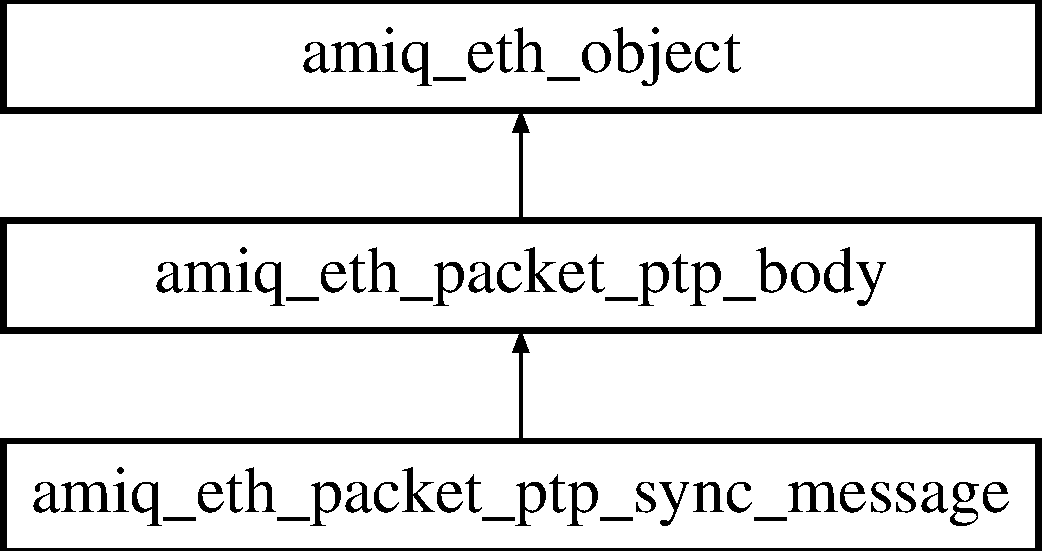
\includegraphics[height=3cm]{classamiq__eth__packet__ptp__sync__message}
\end{center}
\end{figure}
\subsection*{Public Member Functions}
\begin{DoxyCompactItemize}
\item 
\hyperlink{classamiq__eth__packet__ptp__sync__message_ad640a426a022d3a795d2ca5930faf864}{amiq\_\-eth\_\-packet\_\-ptp\_\-sync\_\-message} ()
\item 
\hyperlink{classamiq__eth__packet__ptp__sync__message_aa41c9c0ca4a366b0b16ead16d6777bb0}{$\sim$amiq\_\-eth\_\-packet\_\-ptp\_\-sync\_\-message} ()
\item 
virtual void \hyperlink{classamiq__eth__packet__ptp__sync__message_a5bb7abd15c0d2d2d733f042ad13c898d}{do\_\-pack} (\hyperlink{classamiq__eth__packer}{amiq\_\-eth\_\-packer} \&packer) const 
\item 
virtual void \hyperlink{classamiq__eth__packet__ptp__sync__message_ad0756fb94c7d9ea5ea0da34ca6b41a53}{do\_\-unpack} (\hyperlink{classamiq__eth__packer}{amiq\_\-eth\_\-packer} \&packer)
\item 
virtual void \hyperlink{classamiq__eth__packet__ptp__sync__message_a3eca4a1338800bcac5fdac104f350366}{do\_\-print} (ostream \&out) const 
\end{DoxyCompactItemize}
\subsection*{Public Attributes}
\begin{DoxyCompactItemize}
\item 
\hyperlink{amiq__eth__types_8cpp_add82721f4ff373d2b82269bbf5941032}{amiq\_\-eth\_\-ptp\_\-origin\_\-timestamp} $\ast$ \hyperlink{classamiq__eth__packet__ptp__sync__message_a33121ee506581632ab544ead48cbe342}{origin\_\-timestamp}
\item 
bool \hyperlink{classamiq__eth__packet__ptp__sync__message_ae7f8f44c6b98c23c6f826bbc29e7598c}{print\_\-lists}
\end{DoxyCompactItemize}


\subsection{Detailed Description}


Definition at line 361 of file amiq\_\-eth\_\-packet\_\-ptp.cpp.

\subsection{Constructor \& Destructor Documentation}
\hypertarget{classamiq__eth__packet__ptp__sync__message_ad640a426a022d3a795d2ca5930faf864}{
\index{amiq\_\-eth\_\-packet\_\-ptp\_\-sync\_\-message@{amiq\_\-eth\_\-packet\_\-ptp\_\-sync\_\-message}!amiq\_\-eth\_\-packet\_\-ptp\_\-sync\_\-message@{amiq\_\-eth\_\-packet\_\-ptp\_\-sync\_\-message}}
\index{amiq\_\-eth\_\-packet\_\-ptp\_\-sync\_\-message@{amiq\_\-eth\_\-packet\_\-ptp\_\-sync\_\-message}!amiq_eth_packet_ptp_sync_message@{amiq\_\-eth\_\-packet\_\-ptp\_\-sync\_\-message}}
\subsubsection[{amiq\_\-eth\_\-packet\_\-ptp\_\-sync\_\-message}]{\setlength{\rightskip}{0pt plus 5cm}amiq\_\-eth\_\-packet\_\-ptp\_\-sync\_\-message::amiq\_\-eth\_\-packet\_\-ptp\_\-sync\_\-message ()\hspace{0.3cm}{\ttfamily  \mbox{[}inline\mbox{]}}}}
\label{classamiq__eth__packet__ptp__sync__message_ad640a426a022d3a795d2ca5930faf864}


Definition at line 370 of file amiq\_\-eth\_\-packet\_\-ptp.cpp.

References AMIQ\_\-ETH\_\-PTP\_\-ORIGIN\_\-TIMESTAMP\_\-SIZE, origin\_\-timestamp, and print\_\-lists.\hypertarget{classamiq__eth__packet__ptp__sync__message_aa41c9c0ca4a366b0b16ead16d6777bb0}{
\index{amiq\_\-eth\_\-packet\_\-ptp\_\-sync\_\-message@{amiq\_\-eth\_\-packet\_\-ptp\_\-sync\_\-message}!$\sim$amiq\_\-eth\_\-packet\_\-ptp\_\-sync\_\-message@{$\sim$amiq\_\-eth\_\-packet\_\-ptp\_\-sync\_\-message}}
\index{$\sim$amiq\_\-eth\_\-packet\_\-ptp\_\-sync\_\-message@{$\sim$amiq\_\-eth\_\-packet\_\-ptp\_\-sync\_\-message}!amiq_eth_packet_ptp_sync_message@{amiq\_\-eth\_\-packet\_\-ptp\_\-sync\_\-message}}
\subsubsection[{$\sim$amiq\_\-eth\_\-packet\_\-ptp\_\-sync\_\-message}]{\setlength{\rightskip}{0pt plus 5cm}amiq\_\-eth\_\-packet\_\-ptp\_\-sync\_\-message::$\sim$amiq\_\-eth\_\-packet\_\-ptp\_\-sync\_\-message ()\hspace{0.3cm}{\ttfamily  \mbox{[}inline\mbox{]}}}}
\label{classamiq__eth__packet__ptp__sync__message_aa41c9c0ca4a366b0b16ead16d6777bb0}


Definition at line 376 of file amiq\_\-eth\_\-packet\_\-ptp.cpp.

\subsection{Member Function Documentation}
\hypertarget{classamiq__eth__packet__ptp__sync__message_a5bb7abd15c0d2d2d733f042ad13c898d}{
\index{amiq\_\-eth\_\-packet\_\-ptp\_\-sync\_\-message@{amiq\_\-eth\_\-packet\_\-ptp\_\-sync\_\-message}!do\_\-pack@{do\_\-pack}}
\index{do\_\-pack@{do\_\-pack}!amiq_eth_packet_ptp_sync_message@{amiq\_\-eth\_\-packet\_\-ptp\_\-sync\_\-message}}
\subsubsection[{do\_\-pack}]{\setlength{\rightskip}{0pt plus 5cm}virtual void amiq\_\-eth\_\-packet\_\-ptp\_\-sync\_\-message::do\_\-pack ({\bf amiq\_\-eth\_\-packer} \& {\em packer}) const\hspace{0.3cm}{\ttfamily  \mbox{[}inline, virtual\mbox{]}}}}
\label{classamiq__eth__packet__ptp__sync__message_a5bb7abd15c0d2d2d733f042ad13c898d}


Reimplemented from \hyperlink{classamiq__eth__packet__ptp__body_a3df3ad9b3a4ef7ec42357565d44ede05}{amiq\_\-eth\_\-packet\_\-ptp\_\-body}.

Definition at line 381 of file amiq\_\-eth\_\-packet\_\-ptp.cpp.

References amiq\_\-eth\_\-do\_\-pack(), AMIQ\_\-ETH\_\-PTP\_\-ORIGIN\_\-TIMESTAMP\_\-SIZE, and origin\_\-timestamp.

Referenced by amiq\_\-eth\_\-packet\_\-ptp::pack\_\-body().\hypertarget{classamiq__eth__packet__ptp__sync__message_a3eca4a1338800bcac5fdac104f350366}{
\index{amiq\_\-eth\_\-packet\_\-ptp\_\-sync\_\-message@{amiq\_\-eth\_\-packet\_\-ptp\_\-sync\_\-message}!do\_\-print@{do\_\-print}}
\index{do\_\-print@{do\_\-print}!amiq_eth_packet_ptp_sync_message@{amiq\_\-eth\_\-packet\_\-ptp\_\-sync\_\-message}}
\subsubsection[{do\_\-print}]{\setlength{\rightskip}{0pt plus 5cm}virtual void amiq\_\-eth\_\-packet\_\-ptp\_\-sync\_\-message::do\_\-print (ostream \& {\em out}) const\hspace{0.3cm}{\ttfamily  \mbox{[}inline, virtual\mbox{]}}}}
\label{classamiq__eth__packet__ptp__sync__message_a3eca4a1338800bcac5fdac104f350366}


Reimplemented from \hyperlink{classamiq__eth__packet__ptp__body_a44ff8df4c84f236f8bab792ceb338e6a}{amiq\_\-eth\_\-packet\_\-ptp\_\-body}.

Definition at line 403 of file amiq\_\-eth\_\-packet\_\-ptp.cpp.

References AMIQ\_\-ETH\_\-FIELD\_\-SEPARATOR, AMIQ\_\-ETH\_\-PTP\_\-ORIGIN\_\-TIMESTAMP\_\-SIZE, origin\_\-timestamp, and print\_\-lists.

Referenced by amiq\_\-eth\_\-packet\_\-ptp::do\_\-print().\hypertarget{classamiq__eth__packet__ptp__sync__message_ad0756fb94c7d9ea5ea0da34ca6b41a53}{
\index{amiq\_\-eth\_\-packet\_\-ptp\_\-sync\_\-message@{amiq\_\-eth\_\-packet\_\-ptp\_\-sync\_\-message}!do\_\-unpack@{do\_\-unpack}}
\index{do\_\-unpack@{do\_\-unpack}!amiq_eth_packet_ptp_sync_message@{amiq\_\-eth\_\-packet\_\-ptp\_\-sync\_\-message}}
\subsubsection[{do\_\-unpack}]{\setlength{\rightskip}{0pt plus 5cm}virtual void amiq\_\-eth\_\-packet\_\-ptp\_\-sync\_\-message::do\_\-unpack ({\bf amiq\_\-eth\_\-packer} \& {\em packer})\hspace{0.3cm}{\ttfamily  \mbox{[}inline, virtual\mbox{]}}}}
\label{classamiq__eth__packet__ptp__sync__message_ad0756fb94c7d9ea5ea0da34ca6b41a53}


Reimplemented from \hyperlink{classamiq__eth__packet__ptp__body_a17a10ad537b6553f35b54d2f037d4f0d}{amiq\_\-eth\_\-packet\_\-ptp\_\-body}.

Definition at line 391 of file amiq\_\-eth\_\-packet\_\-ptp.cpp.

References amiq\_\-eth\_\-do\_\-unpack(), AMIQ\_\-ETH\_\-PTP\_\-ORIGIN\_\-TIMESTAMP\_\-SIZE, and origin\_\-timestamp.

Referenced by amiq\_\-eth\_\-packet\_\-ptp::do\_\-unpack().

\subsection{Member Data Documentation}
\hypertarget{classamiq__eth__packet__ptp__sync__message_a33121ee506581632ab544ead48cbe342}{
\index{amiq\_\-eth\_\-packet\_\-ptp\_\-sync\_\-message@{amiq\_\-eth\_\-packet\_\-ptp\_\-sync\_\-message}!origin\_\-timestamp@{origin\_\-timestamp}}
\index{origin\_\-timestamp@{origin\_\-timestamp}!amiq_eth_packet_ptp_sync_message@{amiq\_\-eth\_\-packet\_\-ptp\_\-sync\_\-message}}
\subsubsection[{origin\_\-timestamp}]{\setlength{\rightskip}{0pt plus 5cm}{\bf amiq\_\-eth\_\-ptp\_\-origin\_\-timestamp}$\ast$ {\bf amiq\_\-eth\_\-packet\_\-ptp\_\-sync\_\-message::origin\_\-timestamp}}}
\label{classamiq__eth__packet__ptp__sync__message_a33121ee506581632ab544ead48cbe342}


Definition at line 364 of file amiq\_\-eth\_\-packet\_\-ptp.cpp.

Referenced by amiq\_\-eth\_\-packet\_\-ptp\_\-sync\_\-message(), do\_\-pack(), do\_\-print(), and do\_\-unpack().\hypertarget{classamiq__eth__packet__ptp__sync__message_ae7f8f44c6b98c23c6f826bbc29e7598c}{
\index{amiq\_\-eth\_\-packet\_\-ptp\_\-sync\_\-message@{amiq\_\-eth\_\-packet\_\-ptp\_\-sync\_\-message}!print\_\-lists@{print\_\-lists}}
\index{print\_\-lists@{print\_\-lists}!amiq_eth_packet_ptp_sync_message@{amiq\_\-eth\_\-packet\_\-ptp\_\-sync\_\-message}}
\subsubsection[{print\_\-lists}]{\setlength{\rightskip}{0pt plus 5cm}bool {\bf amiq\_\-eth\_\-packet\_\-ptp\_\-sync\_\-message::print\_\-lists}}}
\label{classamiq__eth__packet__ptp__sync__message_ae7f8f44c6b98c23c6f826bbc29e7598c}


Definition at line 367 of file amiq\_\-eth\_\-packet\_\-ptp.cpp.

Referenced by amiq\_\-eth\_\-packet\_\-ptp\_\-sync\_\-message(), and do\_\-print().

The documentation for this class was generated from the following file:\begin{DoxyCompactItemize}
\item 
/home/cristian.slav/work/amiq/projects/sv/amiq\_\-eth/sc/\hyperlink{amiq__eth__packet__ptp_8cpp}{amiq\_\-eth\_\-packet\_\-ptp.cpp}\end{DoxyCompactItemize}

\hypertarget{classamiq__eth__packet__snap}{
\section{amiq\_\-eth\_\-packet\_\-snap Class Reference}
\label{classamiq__eth__packet__snap}\index{amiq\_\-eth\_\-packet\_\-snap@{amiq\_\-eth\_\-packet\_\-snap}}
}
Inheritance diagram for amiq\_\-eth\_\-packet\_\-snap::\begin{figure}[H]
\begin{center}
\leavevmode
\includegraphics[height=3cm]{classamiq__eth__packet__snap}
\end{center}
\end{figure}
\subsection*{Public Member Functions}
\begin{DoxyCompactItemize}
\item 
\hyperlink{classamiq__eth__packet__snap_a768dde5515c9a9d5ca0cb56b1d01d14b}{amiq\_\-eth\_\-packet\_\-snap} ()
\item 
virtual \hyperlink{classamiq__eth__packet__snap_a4e5486a36616f6fda29c1248796704fb}{$\sim$amiq\_\-eth\_\-packet\_\-snap} ()
\item 
virtual void \hyperlink{classamiq__eth__packet__snap_ace29c0c126f983a5e88ff933f1b34ff6}{do\_\-pack} (\hyperlink{classamiq__eth__packer}{amiq\_\-eth\_\-packer} \&packer) const 
\item 
virtual void \hyperlink{classamiq__eth__packet__snap_a7bb9ce14ff76d5bacb715a53382a7816}{do\_\-unpack} (\hyperlink{classamiq__eth__packer}{amiq\_\-eth\_\-packer} \&packer)
\item 
virtual void \hyperlink{classamiq__eth__packet__snap_a042b049988a9e938cb80acb497cfafe5}{do\_\-pack\_\-for\_\-fcs} (\hyperlink{classamiq__eth__packer}{amiq\_\-eth\_\-packer} \&packer) const 
\item 
virtual void \hyperlink{classamiq__eth__packet__snap_af0ca9e38d460f39767d5abf60f48cee9}{do\_\-print} (ostream \&out) const 
\item 
virtual tlm\_\-generic\_\-payload $\ast$ \hyperlink{classamiq__eth__packet__snap_a99256008f171d933ec625d7957b64270}{to\_\-generic\_\-payload} () const 
\end{DoxyCompactItemize}
\subsection*{Public Attributes}
\begin{DoxyCompactItemize}
\item 
\hyperlink{amiq__eth__types_8cpp_a4d2be172e6524c991fe389337947afc0}{amiq\_\-eth\_\-length\_\-type} \hyperlink{classamiq__eth__packet__snap_aab2892c994afa1c55c560ae287f96f19}{length}
\item 
\hyperlink{amiq__eth__types_8cpp_a3595a0a508d433d383d3e5521fc0b723}{amiq\_\-eth\_\-data} \hyperlink{classamiq__eth__packet__snap_a3472137088bb7bc9085610f4f848527f}{dsap}
\item 
\hyperlink{amiq__eth__types_8cpp_a3595a0a508d433d383d3e5521fc0b723}{amiq\_\-eth\_\-data} \hyperlink{classamiq__eth__packet__snap_a6acbe3de6637a59ffae0b491b8567991}{ssap}
\item 
\hyperlink{amiq__eth__types_8cpp_a3595a0a508d433d383d3e5521fc0b723}{amiq\_\-eth\_\-data} \hyperlink{classamiq__eth__packet__snap_ae4146189e20b5d48c0563c0fa575b578}{ctl}
\item 
\hyperlink{amiq__eth__types_8cpp_a8595e88502ca3eddef1de16991a4a6ef}{amiq\_\-eth\_\-snap\_\-protocol\_\-identifier} \hyperlink{classamiq__eth__packet__snap_a248cb95f457543532684f7a86e2481b3}{protocol\_\-identifier}
\item 
\hyperlink{amiq__eth__types_8cpp_a3595a0a508d433d383d3e5521fc0b723}{amiq\_\-eth\_\-data} $\ast$ \hyperlink{classamiq__eth__packet__snap_aef5354d102ccd32cc521388767ca23fe}{protocol\_\-data}
\item 
\hyperlink{amiq__eth__types_8cpp_adb511dc715b55539c6abdad1de981a9f}{amiq\_\-eth\_\-fcs} \hyperlink{classamiq__eth__packet__snap_aca86c29ed386cc63461db470932b70bc}{fcs}
\end{DoxyCompactItemize}


\subsection{Detailed Description}


Definition at line 32 of file amiq\_\-eth\_\-packet\_\-snap.cpp.

\subsection{Constructor \& Destructor Documentation}
\hypertarget{classamiq__eth__packet__snap_a768dde5515c9a9d5ca0cb56b1d01d14b}{
\index{amiq\_\-eth\_\-packet\_\-snap@{amiq\_\-eth\_\-packet\_\-snap}!amiq\_\-eth\_\-packet\_\-snap@{amiq\_\-eth\_\-packet\_\-snap}}
\index{amiq\_\-eth\_\-packet\_\-snap@{amiq\_\-eth\_\-packet\_\-snap}!amiq_eth_packet_snap@{amiq\_\-eth\_\-packet\_\-snap}}
\subsubsection[{amiq\_\-eth\_\-packet\_\-snap}]{\setlength{\rightskip}{0pt plus 5cm}amiq\_\-eth\_\-packet\_\-snap::amiq\_\-eth\_\-packet\_\-snap ()\hspace{0.3cm}{\ttfamily  \mbox{[}inline\mbox{]}}}}
\label{classamiq__eth__packet__snap_a768dde5515c9a9d5ca0cb56b1d01d14b}


Definition at line 58 of file amiq\_\-eth\_\-packet\_\-snap.cpp.

References NULL, and protocol\_\-data.\hypertarget{classamiq__eth__packet__snap_a4e5486a36616f6fda29c1248796704fb}{
\index{amiq\_\-eth\_\-packet\_\-snap@{amiq\_\-eth\_\-packet\_\-snap}!$\sim$amiq\_\-eth\_\-packet\_\-snap@{$\sim$amiq\_\-eth\_\-packet\_\-snap}}
\index{$\sim$amiq\_\-eth\_\-packet\_\-snap@{$\sim$amiq\_\-eth\_\-packet\_\-snap}!amiq_eth_packet_snap@{amiq\_\-eth\_\-packet\_\-snap}}
\subsubsection[{$\sim$amiq\_\-eth\_\-packet\_\-snap}]{\setlength{\rightskip}{0pt plus 5cm}virtual amiq\_\-eth\_\-packet\_\-snap::$\sim$amiq\_\-eth\_\-packet\_\-snap ()\hspace{0.3cm}{\ttfamily  \mbox{[}inline, virtual\mbox{]}}}}
\label{classamiq__eth__packet__snap_a4e5486a36616f6fda29c1248796704fb}


Definition at line 63 of file amiq\_\-eth\_\-packet\_\-snap.cpp.

References NULL, and protocol\_\-data.

\subsection{Member Function Documentation}
\hypertarget{classamiq__eth__packet__snap_ace29c0c126f983a5e88ff933f1b34ff6}{
\index{amiq\_\-eth\_\-packet\_\-snap@{amiq\_\-eth\_\-packet\_\-snap}!do\_\-pack@{do\_\-pack}}
\index{do\_\-pack@{do\_\-pack}!amiq_eth_packet_snap@{amiq\_\-eth\_\-packet\_\-snap}}
\subsubsection[{do\_\-pack}]{\setlength{\rightskip}{0pt plus 5cm}virtual void amiq\_\-eth\_\-packet\_\-snap::do\_\-pack ({\bf amiq\_\-eth\_\-packer} \& {\em packer}) const\hspace{0.3cm}{\ttfamily  \mbox{[}inline, virtual\mbox{]}}}}
\label{classamiq__eth__packet__snap_ace29c0c126f983a5e88ff933f1b34ff6}


Reimplemented from \hyperlink{classamiq__eth__packet_ab580d89fb44208f5a0fe31443619473e}{amiq\_\-eth\_\-packet}.

Definition at line 69 of file amiq\_\-eth\_\-packet\_\-snap.cpp.

References amiq\_\-eth\_\-do\_\-pack(), ctl, dsap, fcs, length, protocol\_\-data, protocol\_\-identifier, and ssap.\hypertarget{classamiq__eth__packet__snap_a042b049988a9e938cb80acb497cfafe5}{
\index{amiq\_\-eth\_\-packet\_\-snap@{amiq\_\-eth\_\-packet\_\-snap}!do\_\-pack\_\-for\_\-fcs@{do\_\-pack\_\-for\_\-fcs}}
\index{do\_\-pack\_\-for\_\-fcs@{do\_\-pack\_\-for\_\-fcs}!amiq_eth_packet_snap@{amiq\_\-eth\_\-packet\_\-snap}}
\subsubsection[{do\_\-pack\_\-for\_\-fcs}]{\setlength{\rightskip}{0pt plus 5cm}virtual void amiq\_\-eth\_\-packet\_\-snap::do\_\-pack\_\-for\_\-fcs ({\bf amiq\_\-eth\_\-packer} \& {\em packer}) const\hspace{0.3cm}{\ttfamily  \mbox{[}inline, virtual\mbox{]}}}}
\label{classamiq__eth__packet__snap_a042b049988a9e938cb80acb497cfafe5}


Reimplemented from \hyperlink{classamiq__eth__packet_aacbc675df31e2674b5b4c73c9bd9961e}{amiq\_\-eth\_\-packet}.

Definition at line 107 of file amiq\_\-eth\_\-packet\_\-snap.cpp.

References amiq\_\-eth\_\-do\_\-pack(), ctl, dsap, length, protocol\_\-data, protocol\_\-identifier, and ssap.\hypertarget{classamiq__eth__packet__snap_af0ca9e38d460f39767d5abf60f48cee9}{
\index{amiq\_\-eth\_\-packet\_\-snap@{amiq\_\-eth\_\-packet\_\-snap}!do\_\-print@{do\_\-print}}
\index{do\_\-print@{do\_\-print}!amiq_eth_packet_snap@{amiq\_\-eth\_\-packet\_\-snap}}
\subsubsection[{do\_\-print}]{\setlength{\rightskip}{0pt plus 5cm}virtual void amiq\_\-eth\_\-packet\_\-snap::do\_\-print (ostream \& {\em out}) const\hspace{0.3cm}{\ttfamily  \mbox{[}inline, virtual\mbox{]}}}}
\label{classamiq__eth__packet__snap_af0ca9e38d460f39767d5abf60f48cee9}


Reimplemented from \hyperlink{classamiq__eth__packet_aa179c700ae183f1b884a9222a73fed4e}{amiq\_\-eth\_\-packet}.

Definition at line 123 of file amiq\_\-eth\_\-packet\_\-snap.cpp.

References AMIQ\_\-ETH\_\-FIELD\_\-SEPARATOR, ctl, dsap, fcs, amiq\_\-eth\_\-packet::get\_\-correct\_\-fcs(), length, protocol\_\-identifier, and ssap.\hypertarget{classamiq__eth__packet__snap_a7bb9ce14ff76d5bacb715a53382a7816}{
\index{amiq\_\-eth\_\-packet\_\-snap@{amiq\_\-eth\_\-packet\_\-snap}!do\_\-unpack@{do\_\-unpack}}
\index{do\_\-unpack@{do\_\-unpack}!amiq_eth_packet_snap@{amiq\_\-eth\_\-packet\_\-snap}}
\subsubsection[{do\_\-unpack}]{\setlength{\rightskip}{0pt plus 5cm}virtual void amiq\_\-eth\_\-packet\_\-snap::do\_\-unpack ({\bf amiq\_\-eth\_\-packer} \& {\em packer})\hspace{0.3cm}{\ttfamily  \mbox{[}inline, virtual\mbox{]}}}}
\label{classamiq__eth__packet__snap_a7bb9ce14ff76d5bacb715a53382a7816}


Reimplemented from \hyperlink{classamiq__eth__packet_a909eb3860185125564fa530496ed1c9e}{amiq\_\-eth\_\-packet}.

Definition at line 86 of file amiq\_\-eth\_\-packet\_\-snap.cpp.

References amiq\_\-eth\_\-do\_\-unpack(), ctl, dsap, fcs, length, protocol\_\-data, protocol\_\-identifier, and ssap.\hypertarget{classamiq__eth__packet__snap_a99256008f171d933ec625d7957b64270}{
\index{amiq\_\-eth\_\-packet\_\-snap@{amiq\_\-eth\_\-packet\_\-snap}!to\_\-generic\_\-payload@{to\_\-generic\_\-payload}}
\index{to\_\-generic\_\-payload@{to\_\-generic\_\-payload}!amiq_eth_packet_snap@{amiq\_\-eth\_\-packet\_\-snap}}
\subsubsection[{to\_\-generic\_\-payload}]{\setlength{\rightskip}{0pt plus 5cm}virtual tlm\_\-generic\_\-payload$\ast$ amiq\_\-eth\_\-packet\_\-snap::to\_\-generic\_\-payload () const\hspace{0.3cm}{\ttfamily  \mbox{[}inline, virtual\mbox{]}}}}
\label{classamiq__eth__packet__snap_a99256008f171d933ec625d7957b64270}


Reimplemented from \hyperlink{classamiq__eth__packet_a6dd92751d8172eeaa347d71bb415b0d5}{amiq\_\-eth\_\-packet}.

Definition at line 147 of file amiq\_\-eth\_\-packet\_\-snap.cpp.

References AMIQ\_\-ETH\_\-PACKET\_\-SNAP\_\-CODE.

\subsection{Member Data Documentation}
\hypertarget{classamiq__eth__packet__snap_ae4146189e20b5d48c0563c0fa575b578}{
\index{amiq\_\-eth\_\-packet\_\-snap@{amiq\_\-eth\_\-packet\_\-snap}!ctl@{ctl}}
\index{ctl@{ctl}!amiq_eth_packet_snap@{amiq\_\-eth\_\-packet\_\-snap}}
\subsubsection[{ctl}]{\setlength{\rightskip}{0pt plus 5cm}{\bf amiq\_\-eth\_\-data} {\bf amiq\_\-eth\_\-packet\_\-snap::ctl}}}
\label{classamiq__eth__packet__snap_ae4146189e20b5d48c0563c0fa575b578}


Definition at line 46 of file amiq\_\-eth\_\-packet\_\-snap.cpp.

Referenced by do\_\-pack(), do\_\-pack\_\-for\_\-fcs(), do\_\-print(), and do\_\-unpack().\hypertarget{classamiq__eth__packet__snap_a3472137088bb7bc9085610f4f848527f}{
\index{amiq\_\-eth\_\-packet\_\-snap@{amiq\_\-eth\_\-packet\_\-snap}!dsap@{dsap}}
\index{dsap@{dsap}!amiq_eth_packet_snap@{amiq\_\-eth\_\-packet\_\-snap}}
\subsubsection[{dsap}]{\setlength{\rightskip}{0pt plus 5cm}{\bf amiq\_\-eth\_\-data} {\bf amiq\_\-eth\_\-packet\_\-snap::dsap}}}
\label{classamiq__eth__packet__snap_a3472137088bb7bc9085610f4f848527f}


Definition at line 40 of file amiq\_\-eth\_\-packet\_\-snap.cpp.

Referenced by do\_\-pack(), do\_\-pack\_\-for\_\-fcs(), do\_\-print(), and do\_\-unpack().\hypertarget{classamiq__eth__packet__snap_aca86c29ed386cc63461db470932b70bc}{
\index{amiq\_\-eth\_\-packet\_\-snap@{amiq\_\-eth\_\-packet\_\-snap}!fcs@{fcs}}
\index{fcs@{fcs}!amiq_eth_packet_snap@{amiq\_\-eth\_\-packet\_\-snap}}
\subsubsection[{fcs}]{\setlength{\rightskip}{0pt plus 5cm}{\bf amiq\_\-eth\_\-fcs} {\bf amiq\_\-eth\_\-packet\_\-snap::fcs}}}
\label{classamiq__eth__packet__snap_aca86c29ed386cc63461db470932b70bc}


Definition at line 55 of file amiq\_\-eth\_\-packet\_\-snap.cpp.

Referenced by do\_\-pack(), do\_\-print(), and do\_\-unpack().\hypertarget{classamiq__eth__packet__snap_aab2892c994afa1c55c560ae287f96f19}{
\index{amiq\_\-eth\_\-packet\_\-snap@{amiq\_\-eth\_\-packet\_\-snap}!length@{length}}
\index{length@{length}!amiq_eth_packet_snap@{amiq\_\-eth\_\-packet\_\-snap}}
\subsubsection[{length}]{\setlength{\rightskip}{0pt plus 5cm}{\bf amiq\_\-eth\_\-length\_\-type} {\bf amiq\_\-eth\_\-packet\_\-snap::length}}}
\label{classamiq__eth__packet__snap_aab2892c994afa1c55c560ae287f96f19}


Definition at line 37 of file amiq\_\-eth\_\-packet\_\-snap.cpp.

Referenced by do\_\-pack(), do\_\-pack\_\-for\_\-fcs(), do\_\-print(), and do\_\-unpack().\hypertarget{classamiq__eth__packet__snap_aef5354d102ccd32cc521388767ca23fe}{
\index{amiq\_\-eth\_\-packet\_\-snap@{amiq\_\-eth\_\-packet\_\-snap}!protocol\_\-data@{protocol\_\-data}}
\index{protocol\_\-data@{protocol\_\-data}!amiq_eth_packet_snap@{amiq\_\-eth\_\-packet\_\-snap}}
\subsubsection[{protocol\_\-data}]{\setlength{\rightskip}{0pt plus 5cm}{\bf amiq\_\-eth\_\-data}$\ast$ {\bf amiq\_\-eth\_\-packet\_\-snap::protocol\_\-data}}}
\label{classamiq__eth__packet__snap_aef5354d102ccd32cc521388767ca23fe}


Definition at line 52 of file amiq\_\-eth\_\-packet\_\-snap.cpp.

Referenced by amiq\_\-eth\_\-packet\_\-snap(), do\_\-pack(), do\_\-pack\_\-for\_\-fcs(), do\_\-unpack(), and $\sim$amiq\_\-eth\_\-packet\_\-snap().\hypertarget{classamiq__eth__packet__snap_a248cb95f457543532684f7a86e2481b3}{
\index{amiq\_\-eth\_\-packet\_\-snap@{amiq\_\-eth\_\-packet\_\-snap}!protocol\_\-identifier@{protocol\_\-identifier}}
\index{protocol\_\-identifier@{protocol\_\-identifier}!amiq_eth_packet_snap@{amiq\_\-eth\_\-packet\_\-snap}}
\subsubsection[{protocol\_\-identifier}]{\setlength{\rightskip}{0pt plus 5cm}{\bf amiq\_\-eth\_\-snap\_\-protocol\_\-identifier} {\bf amiq\_\-eth\_\-packet\_\-snap::protocol\_\-identifier}}}
\label{classamiq__eth__packet__snap_a248cb95f457543532684f7a86e2481b3}


Definition at line 49 of file amiq\_\-eth\_\-packet\_\-snap.cpp.

Referenced by do\_\-pack(), do\_\-pack\_\-for\_\-fcs(), do\_\-print(), and do\_\-unpack().\hypertarget{classamiq__eth__packet__snap_a6acbe3de6637a59ffae0b491b8567991}{
\index{amiq\_\-eth\_\-packet\_\-snap@{amiq\_\-eth\_\-packet\_\-snap}!ssap@{ssap}}
\index{ssap@{ssap}!amiq_eth_packet_snap@{amiq\_\-eth\_\-packet\_\-snap}}
\subsubsection[{ssap}]{\setlength{\rightskip}{0pt plus 5cm}{\bf amiq\_\-eth\_\-data} {\bf amiq\_\-eth\_\-packet\_\-snap::ssap}}}
\label{classamiq__eth__packet__snap_a6acbe3de6637a59ffae0b491b8567991}


Definition at line 43 of file amiq\_\-eth\_\-packet\_\-snap.cpp.

Referenced by do\_\-pack(), do\_\-pack\_\-for\_\-fcs(), do\_\-print(), and do\_\-unpack().

The documentation for this class was generated from the following file:\begin{DoxyCompactItemize}
\item 
/home/cristian.slav/work/amiq/projects/sv/amiq\_\-eth/sc/\hyperlink{amiq__eth__packet__snap_8cpp}{amiq\_\-eth\_\-packet\_\-snap.cpp}\end{DoxyCompactItemize}

\chapter{File Documentation}
\hypertarget{amiq__eth_8h}{
\section{/home/cristian.slav/work/amiq/projects/sv/amiq\_\-eth/sc/amiq\_\-eth.h File Reference}
\label{amiq__eth_8h}\index{/home/cristian.slav/work/amiq/projects/sv/amiq\_\-eth/sc/amiq\_\-eth.h@{/home/cristian.slav/work/amiq/projects/sv/amiq\_\-eth/sc/amiq\_\-eth.h}}
}
{\ttfamily \#include $<$systemc.h$>$}\par
{\ttfamily \#include \char`\"{}sysc/utils/sc\_\-report.h\char`\"{}}\par
{\ttfamily \#include \char`\"{}amiq\_\-eth\_\-defines.cpp\char`\"{}}\par
{\ttfamily \#include \char`\"{}amiq\_\-eth\_\-ethernet\_\-protocols.cpp\char`\"{}}\par
{\ttfamily \#include \char`\"{}amiq\_\-eth\_\-packer.cpp\char`\"{}}\par
{\ttfamily \#include \char`\"{}amiq\_\-eth\_\-types.cpp\char`\"{}}\par
{\ttfamily \#include \char`\"{}amiq\_\-eth\_\-packet.cpp\char`\"{}}\par
{\ttfamily \#include \char`\"{}amiq\_\-eth\_\-packet\_\-ether\_\-type.cpp\char`\"{}}\par
{\ttfamily \#include \char`\"{}amiq\_\-eth\_\-packet\_\-length.cpp\char`\"{}}\par
{\ttfamily \#include \char`\"{}amiq\_\-eth\_\-packet\_\-pause.cpp\char`\"{}}\par
{\ttfamily \#include \char`\"{}amiq\_\-eth\_\-packet\_\-pfc\_\-pause.cpp\char`\"{}}\par
{\ttfamily \#include \char`\"{}amiq\_\-eth\_\-packet\_\-snap.cpp\char`\"{}}\par
{\ttfamily \#include \char`\"{}amiq\_\-eth\_\-packet\_\-jumbo.cpp\char`\"{}}\par
{\ttfamily \#include \char`\"{}amiq\_\-eth\_\-packet\_\-magic.cpp\char`\"{}}\par
{\ttfamily \#include \char`\"{}amiq\_\-eth\_\-packet\_\-ethernet\_\-configuration\_\-testing.cpp\char`\"{}}\par
{\ttfamily \#include \char`\"{}amiq\_\-eth\_\-packet\_\-ipv4.cpp\char`\"{}}\par
{\ttfamily \#include \char`\"{}amiq\_\-eth\_\-packet\_\-hsr\_\-base.cpp\char`\"{}}\par
{\ttfamily \#include \char`\"{}amiq\_\-eth\_\-packet\_\-hsr\_\-standard.cpp\char`\"{}}\par
{\ttfamily \#include \char`\"{}amiq\_\-eth\_\-packet\_\-fcoe.cpp\char`\"{}}\par
{\ttfamily \#include \char`\"{}amiq\_\-eth\_\-packet\_\-arp.cpp\char`\"{}}\par
{\ttfamily \#include \char`\"{}amiq\_\-eth\_\-packet\_\-ptp.cpp\char`\"{}}\par

\hypertarget{amiq__eth__defines_8cpp}{
\section{/home/cristian.slav/work/amiq/projects/sv/amiq\_\-eth/sc/amiq\_\-eth\_\-defines.cpp File Reference}
\label{amiq__eth__defines_8cpp}\index{/home/cristian.slav/work/amiq/projects/sv/amiq\_\-eth/sc/amiq\_\-eth\_\-defines.cpp@{/home/cristian.slav/work/amiq/projects/sv/amiq\_\-eth/sc/amiq\_\-eth\_\-defines.cpp}}
}
\subsection*{Defines}
\begin{DoxyCompactItemize}
\item 
\#define \hyperlink{amiq__eth__defines_8cpp_a1a81d3983b81172476503f359ce9dfac}{AMIQ\_\-ETH\_\-PREAMBLE\_\-WIDTH}~56
\item 
\#define \hyperlink{amiq__eth__defines_8cpp_a2c8303adb60323cb3917849894a9899c}{AMIQ\_\-ETH\_\-SFD\_\-WIDTH}~8
\item 
\#define \hyperlink{amiq__eth__defines_8cpp_abccf8c7e5f2790d16ce28d956e5ff753}{AMIQ\_\-ETH\_\-ADDRESS\_\-WIDTH}~48
\item 
\#define \hyperlink{amiq__eth__defines_8cpp_a08f3aff9f1eb8058dd8ed6c0834c8ed8}{AMIQ\_\-ETH\_\-LENGTH\_\-TYPE\_\-WIDTH}~16
\item 
\#define \hyperlink{amiq__eth__defines_8cpp_a3dbbbcd385c079790d56fbeb36a7194f}{AMIQ\_\-ETH\_\-FCS\_\-WIDTH}~32
\item 
\#define \hyperlink{amiq__eth__defines_8cpp_accecf3c33c6536745442a8fdcd7b2b5c}{AMIQ\_\-ETH\_\-DATA\_\-WIDTH}~8
\item 
\#define \hyperlink{amiq__eth__defines_8cpp_ac05728e6a241e4e607d58b0fb53398e6}{AMIQ\_\-ETH\_\-EXTENSION\_\-WIDTH}~1
\item 
\#define \hyperlink{amiq__eth__defines_8cpp_a23b2f089a4ec3f350161050925552576}{AMIQ\_\-ETH\_\-MIN\_\-JUMBO\_\-PAYLOAD\_\-SIZE}~1501
\item 
\#define \hyperlink{amiq__eth__defines_8cpp_ad7bf02da973872373bff72dd93934980}{AMIQ\_\-ETH\_\-MAX\_\-JUMBO\_\-PAYLOAD\_\-SIZE}~9000
\item 
\#define \hyperlink{amiq__eth__defines_8cpp_afa9e11f72f8a6149d052fd711b8e21e3}{AMIQ\_\-ETH\_\-PAUSE\_\-PACKET\_\-DESTINATION\_\-ADDRESS}~0x0180C2000001
\item 
\#define \hyperlink{amiq__eth__defines_8cpp_af64e1e91062d942177026f37484d1367}{AMIQ\_\-ETH\_\-PFC\_\-PACKET\_\-DESTINATION\_\-ADDRESS}~0x0180C2000001
\item 
\#define \hyperlink{amiq__eth__defines_8cpp_a341563819d9b55c5a493cb4545309f3e}{AMIQ\_\-ETH\_\-PAUSE\_\-OPCODE\_\-WIDTH}~16
\item 
\#define \hyperlink{amiq__eth__defines_8cpp_a2a4c15ecbab2a6d4d433996d36970c1d}{AMIQ\_\-ETH\_\-PAUSE\_\-PARAMETER\_\-WIDTH}~16
\item 
\#define \hyperlink{amiq__eth__defines_8cpp_adeffa8eccfb426ec430b78c45043f018}{AMIQ\_\-ETH\_\-PAUSE\_\-OPCODE}~0x0001
\item 
\#define \hyperlink{amiq__eth__defines_8cpp_a990996abe206504d41de2b1b25ad79bc}{AMIQ\_\-ETH\_\-PAUSE\_\-PARAMETER\_\-MAX}~0xFFFF
\item 
\#define \hyperlink{amiq__eth__defines_8cpp_abfb674656489ec19d7043e2cb256a117}{AMIQ\_\-ETH\_\-PAUSE\_\-PARAMETER\_\-MIN}~0x0000
\item 
\#define \hyperlink{amiq__eth__defines_8cpp_a3685260c12037630bf6078542c0d21b3}{AMIQ\_\-ETH\_\-PFC\_\-OPCODE\_\-WIDTH}~16
\item 
\#define \hyperlink{amiq__eth__defines_8cpp_acc4b849bcb0d8226b6fba17a91c33dee}{AMIQ\_\-ETH\_\-PFC\_\-OPCODE}~0x0101
\item 
\#define \hyperlink{amiq__eth__defines_8cpp_aeca682c1c5c899656b2479b0f285a0c5}{AMIQ\_\-ETH\_\-PFC\_\-CLASS\_\-ENABLE\_\-VECTOR\_\-WIDTH}~16
\item 
\#define \hyperlink{amiq__eth__defines_8cpp_a7a27841b7d2ce9d34fa84fe1ba164fea}{AMIQ\_\-ETH\_\-PFC\_\-CLASS\_\-ENABLE\_\-VECTOR\_\-MAX}~0x0000
\item 
\#define \hyperlink{amiq__eth__defines_8cpp_a2b1268f5c17941574942dedf550a8bce}{AMIQ\_\-ETH\_\-PFC\_\-CLASS\_\-ENABLE\_\-VECTOR\_\-MIN}~0x00FF
\item 
\#define \hyperlink{amiq__eth__defines_8cpp_a6bea84e0e6714654c77df55cab594ad2}{AMIQ\_\-ETH\_\-PFC\_\-NUMBER\_\-OF\_\-PARAMETERS}~8
\item 
\#define \hyperlink{amiq__eth__defines_8cpp_a9fa828d7723c567f639fef7b03eb873f}{AMIQ\_\-ETH\_\-PFC\_\-PARAMETER\_\-WIDTH}~16
\item 
\#define \hyperlink{amiq__eth__defines_8cpp_a4a36ab23cfdf955ce2f51771836dff10}{AMIQ\_\-ETH\_\-PFC\_\-PARAMETER\_\-MAX}~0xFFFF
\item 
\#define \hyperlink{amiq__eth__defines_8cpp_a202002be468883cdf69f9c179eae4be1}{AMIQ\_\-ETH\_\-PFC\_\-PARAMETER\_\-MIN}~0x0000
\item 
\#define \hyperlink{amiq__eth__defines_8cpp_a27e6a4837bba8be284c6834b6724c1a1}{AMIQ\_\-ETH\_\-PAYLOAD\_\-SIZE\_\-MIN}~46
\item 
\#define \hyperlink{amiq__eth__defines_8cpp_a6835fa2c6a5e9092b06a4889dd49746d}{AMIQ\_\-ETH\_\-PAYLOAD\_\-SIZE\_\-MAX}~1500
\item 
\#define \hyperlink{amiq__eth__defines_8cpp_a767097e15d1a1cb5357324a920ccdb8d}{AMIQ\_\-ETH\_\-MAGIC\_\-PACKET\_\-DEFAULT\_\-ADDRESS\_\-REPETITIONS}~6
\item 
\#define \hyperlink{amiq__eth__defines_8cpp_aa5567531807ac00cb5f942effd9261df}{AMIQ\_\-ETH\_\-MAGIC\_\-PACKET\_\-PATTERN\_\-WIDTH}~48
\item 
\#define \hyperlink{amiq__eth__defines_8cpp_afa19898f0b351641ef75ba5beb672539}{AMIQ\_\-ETH\_\-DEFAULT\_\-MAGIC\_\-PACKET\_\-PATTERN}~0xFFFFFF
\item 
\#define \hyperlink{amiq__eth__defines_8cpp_a108698cb26f5589dcfa459310b318446}{AMIQ\_\-ETH\_\-DEFAULT\_\-SNAP\_\-PACKET\_\-DSAP}~0xAA
\item 
\#define \hyperlink{amiq__eth__defines_8cpp_a266b680baae8b66ae868d3c9602be684}{AMIQ\_\-ETH\_\-DEFAULT\_\-SNAP\_\-PACKET\_\-SSAP}~0xAA
\item 
\#define \hyperlink{amiq__eth__defines_8cpp_afd36706f31e60aa8a867341a94b94e53}{AMIQ\_\-ETH\_\-DEFAULT\_\-SNAP\_\-PACKET\_\-CTL}~0x03
\item 
\#define \hyperlink{amiq__eth__defines_8cpp_ae762fc39125a67a962fbea6f4ba2f566}{AMIQ\_\-ETH\_\-SNAP\_\-PACKET\_\-PROTOCOL\_\-IDENTIFIER\_\-WIDTH}~40
\item 
\#define \hyperlink{amiq__eth__defines_8cpp_a5490a4970da11306aef1bed5cd2e6446}{AMIQ\_\-ETH\_\-JUMBO\_\-CLIENT\_\-DATA\_\-SIZE\_\-WIDTH}~32
\item 
\#define \hyperlink{amiq__eth__defines_8cpp_aa248346edfbcbb489b18fe73e31cacfc}{AMIQ\_\-ETH\_\-MAGIC\_\-CLIENT\_\-DATA\_\-SIZE\_\-WIDTH}~32
\item 
\#define \hyperlink{amiq__eth__defines_8cpp_a070d2ce7b6bb7e5c05602aa8c308d0c4}{NULL}~0
\item 
\#define \hyperlink{amiq__eth__defines_8cpp_adc826a1ca80fe74b62a6f2d740218b20}{AMIQ\_\-ETH\_\-MAGIC\_\-PACKET\_\-SYNCH\_\-STREAM\_\-WIDTH}~48
\item 
\#define \hyperlink{amiq__eth__defines_8cpp_a49a0bd5a38e25455911b30f8b327439f}{AMIQ\_\-ETH\_\-MAGIC\_\-PACKET\_\-TARGET\_\-MAC\_\-REPETITIONS}~6
\item 
\#define \hyperlink{amiq__eth__defines_8cpp_acc5a795332ae57b8fc75a0249b722f3b}{AMIQ\_\-ETH\_\-MAGIC\_\-PACKET\_\-SYNCH\_\-STREAM}~0xFFFFFFFFFFFF
\item 
\#define \hyperlink{amiq__eth__defines_8cpp_aeb0e21c96a7d60fd2dd04687593aa2d0}{AMIQ\_\-ETH\_\-ETHERNET\_\-CONFIGURATION\_\-TESTING\_\-SKIPCOUNT\_\-WIDTH}~16
\item 
\#define \hyperlink{amiq__eth__defines_8cpp_a8b1bfc9c81b655acad0bb1700c2574fc}{AMIQ\_\-ETH\_\-ETHERNET\_\-CONFIGURATION\_\-TESTING\_\-FUNCTION\_\-WIDTH}~16
\item 
\#define \hyperlink{amiq__eth__defines_8cpp_a23847e0991633cb478e0750a0255cdbc}{AMIQ\_\-ETH\_\-ETHERNET\_\-CONFIGURATION\_\-TESTING\_\-REPLY\_\-FUNCTION}~1
\item 
\#define \hyperlink{amiq__eth__defines_8cpp_a17e9e02c762f507286f90f637d6a414b}{AMIQ\_\-ETH\_\-ETHERNET\_\-CONFIGURATION\_\-TESTING\_\-FORWARD\_\-FUNCTION}~2
\item 
\#define \hyperlink{amiq__eth__defines_8cpp_a86439f3e717bf9d1091dfc1c643cbfb5}{AMIQ\_\-ETH\_\-ETHERNET\_\-CONFIGURATION\_\-TESTING\_\-SKIPCOUNT\_\-MAX}~1498
\item 
\#define \hyperlink{amiq__eth__defines_8cpp_ad51b62e3d582337e818507cda8283c17}{AMIQ\_\-ETH\_\-ETHERNET\_\-CONFIGURATION\_\-TESTING\_\-DATA\_\-MAX}~1496
\item 
\#define \hyperlink{amiq__eth__defines_8cpp_a574d4db26b0c3e28620d6fc4881f9d11}{AMIQ\_\-ETH\_\-ETHERNET\_\-CONFIGURATION\_\-TESTING\_\-DATA\_\-MIN}~42
\item 
\#define \hyperlink{amiq__eth__defines_8cpp_aa244b3b627be0d51d9df8373df4ad1fd}{AMIQ\_\-ETH\_\-HSR\_\-PATH\_\-WIDTH}~4
\item 
\#define \hyperlink{amiq__eth__defines_8cpp_ab026edf610a5263aab13dbf590bc17d4}{AMIQ\_\-ETH\_\-HSR\_\-STANDARD\_\-SIZE\_\-WIDTH}~12
\item 
\#define \hyperlink{amiq__eth__defines_8cpp_ac96848aeea7313493d2e8d5e83884ef7}{AMIQ\_\-ETH\_\-HSR\_\-STANDARD\_\-SEQ\_\-WIDTH}~16
\item 
\#define \hyperlink{amiq__eth__defines_8cpp_a0cb5e45355dc2ddb7a8ed3640500759c}{AMIQ\_\-ETH\_\-HSR\_\-STANDARD\_\-PROTOCOL\_\-WIDTH}~16
\item 
\#define \hyperlink{amiq__eth__defines_8cpp_aef465453e6e88d10161c1019dc3d0f8e}{AMIQ\_\-ETH\_\-HSR\_\-STANDARD\_\-LPDU\_\-MAX}~1500
\item 
\#define \hyperlink{amiq__eth__defines_8cpp_aee14c2d36f512d6b0e1c3577d46dced6}{AMIQ\_\-ETH\_\-HSR\_\-STANDARD\_\-LPDU\_\-MIN}~40
\item 
\#define \hyperlink{amiq__eth__defines_8cpp_acb9fafef374cd7ac44fae90838c9090b}{AMIQ\_\-ETH\_\-PACKET\_\-MAGIC\_\-CODE}~0x00000000
\item 
\#define \hyperlink{amiq__eth__defines_8cpp_aa0368ffc00ee7bc17f217d4e893f08fe}{AMIQ\_\-ETH\_\-PACKET\_\-JUMBO\_\-CODE}~0x00000001
\item 
\#define \hyperlink{amiq__eth__defines_8cpp_ad30476f221687c3d9db235c8a7dc938c}{AMIQ\_\-ETH\_\-PACKET\_\-SNAP\_\-CODE}~0x00000002
\item 
\#define \hyperlink{amiq__eth__defines_8cpp_a7f7ba7c9afdae6613eed080dce6613de}{AMIQ\_\-ETH\_\-PACKET\_\-PAUSE\_\-CODE}~0x00000003
\item 
\#define \hyperlink{amiq__eth__defines_8cpp_a6d2e405af406d4dc51823d788a23d9a1}{AMIQ\_\-ETH\_\-PACKET\_\-PFC\_\-PAUSE\_\-CODE}~0x00000004
\item 
\#define \hyperlink{amiq__eth__defines_8cpp_a0cb2bca9a0f41affe9927246d4a8bf2b}{AMIQ\_\-ETH\_\-PACKET\_\-LENGTH\_\-CODE}~0x00000005
\item 
\#define \hyperlink{amiq__eth__defines_8cpp_aeae4c706f718952b4bb59106450fa937}{AMIQ\_\-ETH\_\-PACKET\_\-ETHERNET\_\-CONFIGURATION\_\-TESTING\_\-CODE}~0x00000006
\item 
\#define \hyperlink{amiq__eth__defines_8cpp_acf7f68b41052a54ad1bdf087392b5b62}{AMIQ\_\-ETH\_\-PACKET\_\-IPV4\_\-CODE}~0x00000007
\item 
\#define \hyperlink{amiq__eth__defines_8cpp_ab3c7c45c0d2ae2b783aa92a7f9379f9c}{AMIQ\_\-ETH\_\-PACKET\_\-HSR\_\-STANDARD\_\-CODE}~0x00000008
\item 
\#define \hyperlink{amiq__eth__defines_8cpp_aa5e74f0f82e89c173aa162a69f2ec70d}{AMIQ\_\-ETH\_\-PACKET\_\-ARP\_\-CODE}~0x00000009
\item 
\#define \hyperlink{amiq__eth__defines_8cpp_a31f57f297010390fc9fd6aa782857c80}{AMIQ\_\-ETH\_\-PACKET\_\-FCOE\_\-CODE}~0x0000000A
\item 
\#define \hyperlink{amiq__eth__defines_8cpp_ac41972a0c368cb1f8e9118ec21a95130}{AMIQ\_\-ETH\_\-PACKET\_\-PTP\_\-CODE}~0x0000000C
\item 
\#define \hyperlink{amiq__eth__defines_8cpp_ab1211030ba5e6916d7229fb610225935}{AMIQ\_\-ETH\_\-FIELD\_\-SEPARATOR}~\char`\"{}, \char`\"{}
\item 
\#define \hyperlink{amiq__eth__defines_8cpp_ac2c6387561f1a6f1ebd262849c45791d}{AMIQ\_\-ETH\_\-IPV4\_\-HEADER\_\-VERSION\_\-VALUE}~4
\item 
\#define \hyperlink{amiq__eth__defines_8cpp_ad629d1f18e8800766fd32201ecc6c92d}{AMIQ\_\-ETH\_\-IPV4\_\-HEADER\_\-VERSION\_\-WIDTH}~4
\item 
\#define \hyperlink{amiq__eth__defines_8cpp_abfe8c7e00871d24cac259ca154ba0e31}{AMIQ\_\-ETH\_\-IPV4\_\-HEADER\_\-IHL\_\-WIDTH}~4
\item 
\#define \hyperlink{amiq__eth__defines_8cpp_a7d362806c7eb21b35b93a40067370d45}{AMIQ\_\-ETH\_\-IPV4\_\-HEADER\_\-DSCP\_\-WIDTH}~6
\item 
\#define \hyperlink{amiq__eth__defines_8cpp_a84d79bb67e300d361c5777635bcb67ef}{AMIQ\_\-ETH\_\-IPV4\_\-HEADER\_\-ECN\_\-WIDTH}~2
\item 
\#define \hyperlink{amiq__eth__defines_8cpp_af86ff15ea3a4e15d64c07e42543cc093}{AMIQ\_\-ETH\_\-IPV4\_\-HEADER\_\-TOTAL\_\-LENGTH\_\-WIDTH}~16
\item 
\#define \hyperlink{amiq__eth__defines_8cpp_aa3e975b4a8154c41193314ed736fe28c}{AMIQ\_\-ETH\_\-IPV4\_\-HEADER\_\-IDENTIFICATION\_\-WIDTH}~16
\item 
\#define \hyperlink{amiq__eth__defines_8cpp_a3c00a30ba46fb5fe9b2d78f541ff05f9}{AMIQ\_\-ETH\_\-IPV4\_\-HEADER\_\-FLAGS\_\-WIDTH}~3
\item 
\#define \hyperlink{amiq__eth__defines_8cpp_a94dd4e3c9ce2d6ed9cfce9d4ef0ae990}{AMIQ\_\-ETH\_\-IPV4\_\-HEADER\_\-FRAGMENT\_\-OFFSET\_\-WIDTH}~13
\item 
\#define \hyperlink{amiq__eth__defines_8cpp_ad8e20bfc82b2877b495bdbd0e17f2f1b}{AMIQ\_\-ETH\_\-IPV4\_\-HEADER\_\-TTL\_\-WIDTH}~8
\item 
\#define \hyperlink{amiq__eth__defines_8cpp_acf4ddfde34ffa3163669349164fe9485}{AMIQ\_\-ETH\_\-IPV4\_\-HEADER\_\-PROTOCOL\_\-WIDTH}~8
\item 
\#define \hyperlink{amiq__eth__defines_8cpp_a6e7db673c9da36f4387727139f8f7252}{AMIQ\_\-ETH\_\-IPV4\_\-HEADER\_\-CHECKSUM\_\-WIDTH}~16
\item 
\#define \hyperlink{amiq__eth__defines_8cpp_a763f1b92ade7928c1413e8a980a4e3f9}{AMIQ\_\-ETH\_\-IPV4\_\-HEADER\_\-SOURCE\_\-IP\_\-ADDRESS\_\-WIDTH}~32
\item 
\#define \hyperlink{amiq__eth__defines_8cpp_a61372d6d90fd5e4adccc710f07bd61c6}{AMIQ\_\-ETH\_\-IPV4\_\-HEADER\_\-DESTINATION\_\-IP\_\-ADDRESS\_\-WIDTH}~32
\item 
\#define \hyperlink{amiq__eth__defines_8cpp_a88ad7062339d39adeabcd62f1df35942}{AMIQ\_\-ETH\_\-IPV4\_\-HEADER\_\-OPTION\_\-WIDTH}~32
\item 
\#define \hyperlink{amiq__eth__defines_8cpp_a42938ed66e6a6962143b0f521a545e1d}{AMIQ\_\-ETH\_\-ETHERNET\_\-CONFIGURATION\_\-TESTING\_\-DATA\_\-SIZE\_\-WIDTH}~32
\item 
\#define \hyperlink{amiq__eth__defines_8cpp_aee51e157bdc266357ebd0f65aa17caf4}{AMIQ\_\-ETH\_\-CRC32\_\-CCITT\_\-SEED}~0xFFFFFFFF
\item 
\#define \hyperlink{amiq__eth__defines_8cpp_a4b27c3257c8f07f770f4847327ae420f}{AMIQ\_\-ETH\_\-DEFAULT\_\-MIN\_\-FRAME\_\-SIZE}~64
\item 
\#define \hyperlink{amiq__eth__defines_8cpp_a6ff04512993f3236992c59e8bf5f043f}{AMIQ\_\-ETH\_\-FCOE\_\-VERSION\_\-WIDTH}~4
\item 
\#define \hyperlink{amiq__eth__defines_8cpp_a99f1b5f475ecda5e56e21757268e493e}{AMIQ\_\-ETH\_\-FCOE\_\-RESERVED\_\-BEFORE\_\-SOF\_\-SIZE}~100
\item 
\#define \hyperlink{amiq__eth__defines_8cpp_ad4a329c2640847cda31c39ecea7dc11e}{AMIQ\_\-ETH\_\-FCOE\_\-SOF\_\-WIDTH}~8
\item 
\#define \hyperlink{amiq__eth__defines_8cpp_ace627f7271b445c976986e405f1a6f53}{AMIQ\_\-ETH\_\-FCOE\_\-SOFf}~0x28
\item 
\#define \hyperlink{amiq__eth__defines_8cpp_a2b1ab7e92d265d438b267777c6774c25}{AMIQ\_\-ETH\_\-FCOE\_\-SOFi2}~0x2D
\item 
\#define \hyperlink{amiq__eth__defines_8cpp_ac0d9e0333ad322935cde28822ef1885c}{AMIQ\_\-ETH\_\-FCOE\_\-SOFn2}~0x35
\item 
\#define \hyperlink{amiq__eth__defines_8cpp_a278fb0488d88e24376eaaaf1fb21b236}{AMIQ\_\-ETH\_\-FCOE\_\-SOFi3}~0x2E
\item 
\#define \hyperlink{amiq__eth__defines_8cpp_a90a23ed013d6d6fa393654ac773ee68b}{AMIQ\_\-ETH\_\-FCOE\_\-SOFn3}~0x36
\item 
\#define \hyperlink{amiq__eth__defines_8cpp_ab4bd95da9601289e5c40d637e8577d6a}{AMIQ\_\-ETH\_\-FCOE\_\-SOFi4}~0x29
\item 
\#define \hyperlink{amiq__eth__defines_8cpp_a1fe1b576a2df651a69cd8ee48cec4189}{AMIQ\_\-ETH\_\-FCOE\_\-SOFn4}~0x31
\item 
\#define \hyperlink{amiq__eth__defines_8cpp_adcc7e8826c480a83907dbe732206ed27}{AMIQ\_\-ETH\_\-FCOE\_\-SOFc4}~0x39
\item 
\#define \hyperlink{amiq__eth__defines_8cpp_ad26f285c722c83f106400630b719f4ba}{AMIQ\_\-ETH\_\-ARP\_\-HTYPE\_\-WIDTH}~16
\item 
\#define \hyperlink{amiq__eth__defines_8cpp_ae3b240d571b148205ea1449462d6c2ca}{AMIQ\_\-ETH\_\-ARP\_\-PTYPE\_\-WIDTH}~16
\item 
\#define \hyperlink{amiq__eth__defines_8cpp_a481918457e2040e094fc539c342cdb72}{AMIQ\_\-ETH\_\-ARP\_\-HLEN\_\-WIDTH}~8
\item 
\#define \hyperlink{amiq__eth__defines_8cpp_aeb0da3d1f14520d3033726d5a09388a1}{AMIQ\_\-ETH\_\-ARP\_\-PLEN\_\-WIDTH}~8
\item 
\#define \hyperlink{amiq__eth__defines_8cpp_aa5eb7724f6ad1b7cecfff3185eb5110a}{AMIQ\_\-ETH\_\-ARP\_\-OPER\_\-WIDTH}~16
\item 
\#define \hyperlink{amiq__eth__defines_8cpp_aad9f115fc0f3bfc48032ad0d647e8ece}{AMIQ\_\-ETH\_\-ARP\_\-SHA\_\-WIDTH}~48
\item 
\#define \hyperlink{amiq__eth__defines_8cpp_a2331f4d444370cc551fa8b4cc373ef49}{AMIQ\_\-ETH\_\-ARP\_\-SPA\_\-WIDTH}~32
\item 
\#define \hyperlink{amiq__eth__defines_8cpp_afddaccb8a0d90ac49ccc74635bf24e15}{AMIQ\_\-ETH\_\-ARP\_\-THA\_\-WIDTH}~48
\item 
\#define \hyperlink{amiq__eth__defines_8cpp_af5dee84f59591775a044845b70f915a2}{AMIQ\_\-ETH\_\-ARP\_\-TPA\_\-WIDTH}~32
\item 
\#define \hyperlink{amiq__eth__defines_8cpp_a8dcae98b60085af8f7613069e5f5dc24}{AMIQ\_\-ETH\_\-PTP\_\-TRANSPORT\_\-SPECIFIC\_\-WIDTH}~4
\item 
\#define \hyperlink{amiq__eth__defines_8cpp_a48582d1a3ba03d80016c1f3b39056f9a}{AMIQ\_\-ETH\_\-PTP\_\-IN\_\-IEEE1588}~0
\item 
\#define \hyperlink{amiq__eth__defines_8cpp_a51e41e76a4c7d5afcf8d92265f1e67fc}{AMIQ\_\-ETH\_\-PTP\_\-IN\_\-802\_\-1\_\-AS}~1
\item 
\#define \hyperlink{amiq__eth__defines_8cpp_a230efd1fdbe4ed6d7ad3c87eee2d957a}{AMIQ\_\-ETH\_\-PTP\_\-MESSAGE\_\-TYPE\_\-WIDTH}~4
\item 
\#define \hyperlink{amiq__eth__defines_8cpp_a662f325a8e651017a813d6b97271eae3}{AMIQ\_\-ETH\_\-PTP\_\-SYNCMESSAGE}~0
\item 
\#define \hyperlink{amiq__eth__defines_8cpp_a500e851df3501203db833559bd7d830a}{AMIQ\_\-ETH\_\-PTP\_\-DELAY\_\-REQMESSAGE}~1
\item 
\#define \hyperlink{amiq__eth__defines_8cpp_acb211fba6f89c9ef77929e558219a777}{AMIQ\_\-ETH\_\-PTP\_\-PDELAY\_\-REQMESSAGE}~2
\item 
\#define \hyperlink{amiq__eth__defines_8cpp_a73dd958fb399495edeea4b67040bc560}{AMIQ\_\-ETH\_\-PTP\_\-PDELAY\_\-RESPMESSAGE}~3
\item 
\#define \hyperlink{amiq__eth__defines_8cpp_ae805212cac29aac3fd98e89798fbc7d8}{AMIQ\_\-ETH\_\-PTP\_\-FOLLOW\_\-UPMESSAGE}~8
\item 
\#define \hyperlink{amiq__eth__defines_8cpp_a84b01da2158ebcff71cf2f3d66d23db7}{AMIQ\_\-ETH\_\-PTP\_\-DELAY\_\-RESPMESSAGE}~9
\item 
\#define \hyperlink{amiq__eth__defines_8cpp_ab1529a1650bc7aa37c842dfa3e2e38bd}{AMIQ\_\-ETH\_\-PTP\_\-PDELAY\_\-RESP\_\-FOLLOW\_\-UPMESSAGE}~10
\item 
\#define \hyperlink{amiq__eth__defines_8cpp_a8c56d4cff906ab2e6b60306a1ad0baf2}{AMIQ\_\-ETH\_\-PTP\_\-ANNOUNCEMESSAGE}~11
\item 
\#define \hyperlink{amiq__eth__defines_8cpp_ad23ff06cd2d7d2d775a51b43088c6c46}{AMIQ\_\-ETH\_\-PTP\_\-SIGNALLINGMESSAGE}~12
\item 
\#define \hyperlink{amiq__eth__defines_8cpp_af45f867245f693e3b2135e502c60c147}{AMIQ\_\-ETH\_\-PTP\_\-MANAGEMENTMESSAGE}~13
\item 
\#define \hyperlink{amiq__eth__defines_8cpp_a48783653b9c0a79ec31154ed3a73a737}{AMIQ\_\-ETH\_\-PTP\_\-SYNCMESSAGE\_\-CTRL}~0
\item 
\#define \hyperlink{amiq__eth__defines_8cpp_a5346311ed591d2a5d2a06db096ad6b67}{AMIQ\_\-ETH\_\-PTP\_\-DELAY\_\-REQMESSAGE\_\-CTRL}~1
\item 
\#define \hyperlink{amiq__eth__defines_8cpp_aaaaca65c91f48c8b850fd5f26180f22f}{AMIQ\_\-ETH\_\-PTP\_\-FOLLOW\_\-UPMESSAGE\_\-CTRL}~2
\item 
\#define \hyperlink{amiq__eth__defines_8cpp_a235a636123728a3149a19a735c3f19fb}{AMIQ\_\-ETH\_\-PTP\_\-DELAY\_\-RESPMESSAGE\_\-CTRL}~3
\item 
\#define \hyperlink{amiq__eth__defines_8cpp_a64ab3cdcb37896f6bb615cd8d8b93b98}{AMIQ\_\-ETH\_\-PTP\_\-MANAGEMENTMESSAGE\_\-CTRL}~4
\item 
\#define \hyperlink{amiq__eth__defines_8cpp_a45bd25abe09af2e132487c883cfb4211}{AMIQ\_\-ETH\_\-PTP\_\-RESERVED\_\-WIDTH}~1
\item 
\#define \hyperlink{amiq__eth__defines_8cpp_a8e4be2349c3f85790dda4681b79a5f94}{AMIQ\_\-ETH\_\-PTP\_\-RESERVED\_\-1\_\-WIDTH}~4
\item 
\#define \hyperlink{amiq__eth__defines_8cpp_af8bef8f4e0edde9756e696ba5e3a73d3}{AMIQ\_\-ETH\_\-PTP\_\-VERSION\_\-WIDTH}~4
\item 
\#define \hyperlink{amiq__eth__defines_8cpp_a0cc3a24b4d95c2ad5af9150e545ea1e1}{AMIQ\_\-ETH\_\-PTP\_\-MESSAGE\_\-LENGTH\_\-WIDTH}~16
\item 
\#define \hyperlink{amiq__eth__defines_8cpp_a051f1d841c8cd6cf193773b931e3d377}{AMIQ\_\-ETH\_\-PTP\_\-DOMAIN\_\-NUMBER\_\-WIDTH}~8
\item 
\#define \hyperlink{amiq__eth__defines_8cpp_a7f28f65c97e4a94a90b73354d9d24101}{AMIQ\_\-ETH\_\-PTP\_\-RESERVED\_\-2\_\-WIDTH}~8
\item 
\#define \hyperlink{amiq__eth__defines_8cpp_a2e51c99a6fc602bc0c7229f285de0c08}{AMIQ\_\-ETH\_\-PTP\_\-FLAGS\_\-WIDTH}~16
\item 
\#define \hyperlink{amiq__eth__defines_8cpp_a37d4fc090e820610019d9b1f5eef89ff}{AMIQ\_\-ETH\_\-PTP\_\-CORRECTION\_\-FIELD\_\-WIDTH}~64
\item 
\#define \hyperlink{amiq__eth__defines_8cpp_a5aa8b80a95d6c1ce70c55d1951087e02}{AMIQ\_\-ETH\_\-PTP\_\-RESERVED\_\-3\_\-WIDTH}~32
\item 
\#define \hyperlink{amiq__eth__defines_8cpp_a4f68590e296a39ac5618e9e4f7bbe165}{AMIQ\_\-ETH\_\-PTP\_\-SOURCE\_\-PORT\_\-IDENTITY\_\-WIDTH}~8
\item 
\#define \hyperlink{amiq__eth__defines_8cpp_aa1b87a069ab41f7ad9bb42e005c8b4d3}{AMIQ\_\-ETH\_\-PTP\_\-SOURCE\_\-PORT\_\-IDENTITY\_\-SIZE}~10
\item 
\#define \hyperlink{amiq__eth__defines_8cpp_ae0a44e684bbf78903b6689d0cd08f469}{AMIQ\_\-ETH\_\-PTP\_\-SEQUENCE\_\-ID\_\-WIDTH}~16
\item 
\#define \hyperlink{amiq__eth__defines_8cpp_a71db0d479447b6bc1a1c0d8155d21d49}{AMIQ\_\-ETH\_\-PTP\_\-CONTROL\_\-FIELD\_\-WIDTH}~8
\item 
\#define \hyperlink{amiq__eth__defines_8cpp_ad63cfda69c5b8cbae0f675044ac2b264}{AMIQ\_\-ETH\_\-PTP\_\-LOG\_\-MESSAGE\_\-WIDTH}~8
\item 
\#define \hyperlink{amiq__eth__defines_8cpp_ac6453a8efa0715a273accceffa1c7578}{AMIQ\_\-ETH\_\-PTP\_\-ORIGIN\_\-TIMESTAMP\_\-WIDTH}~8
\item 
\#define \hyperlink{amiq__eth__defines_8cpp_a9b820e85aa81331296e3423c6615d6bf}{AMIQ\_\-ETH\_\-PTP\_\-ORIGIN\_\-TIMESTAMP\_\-SIZE}~10
\item 
\#define \hyperlink{amiq__eth__defines_8cpp_ab2633cc982f8cf52f6614ac6c0c545b8}{AMIQ\_\-ETH\_\-PTP\_\-ANNOUNCE\_\-MESSAGE\_\-CURRENT\_\-UTC\_\-OFFSET\_\-WIDTH}~16
\item 
\#define \hyperlink{amiq__eth__defines_8cpp_a0739516c5664d1134752dbb9bf55d07a}{AMIQ\_\-ETH\_\-PTP\_\-ANNOUNCE\_\-MESSAGE\_\-RESERVED\_\-WIDTH}~8
\item 
\#define \hyperlink{amiq__eth__defines_8cpp_a5385fbf9f147ce7557bb80e6b6f74e62}{AMIQ\_\-ETH\_\-PTP\_\-ANNOUNCE\_\-MESSAGE\_\-GRANDMASTER\_\-PRIORITY\_\-1\_\-WIDTH}~8
\item 
\#define \hyperlink{amiq__eth__defines_8cpp_a4cc22af6abc23f550de4d953fdc99de2}{AMIQ\_\-ETH\_\-PTP\_\-ANNOUNCE\_\-MESSAGE\_\-GRANDMASTER\_\-CLOCK\_\-QUALITY\_\-WIDTH}~32
\item 
\#define \hyperlink{amiq__eth__defines_8cpp_a28c7eb0034a08532c91cb26ebc168f5a}{AMIQ\_\-ETH\_\-PTP\_\-ANNOUNCE\_\-MESSAGE\_\-GRANDMASTER\_\-PRIORITY\_\-2\_\-WIDTH}~8
\item 
\#define \hyperlink{amiq__eth__defines_8cpp_a97a945734cb9404ac2ff73be1d3a029c}{AMIQ\_\-ETH\_\-PTP\_\-ANNOUNCE\_\-MESSAGE\_\-GRANDMASTER\_\-IDENTITY\_\-WIDTH}~64
\item 
\#define \hyperlink{amiq__eth__defines_8cpp_a75bf99054424ff0cdbcf0282036f78df}{AMIQ\_\-ETH\_\-PTP\_\-ANNOUNCE\_\-MESSAGE\_\-STEPS\_\-REMOVED\_\-WIDTH}~16
\item 
\#define \hyperlink{amiq__eth__defines_8cpp_a54dff504d4fed6067070114df0e0612f}{AMIQ\_\-ETH\_\-PTP\_\-ANNOUNCE\_\-MESSAGE\_\-TIME\_\-SOURCE\_\-WIDTH}~8
\item 
\#define \hyperlink{amiq__eth__defines_8cpp_a8d6e068db906f7468ea3c66a2c7f10ae}{AMIQ\_\-ETH\_\-FCOE\_\-EOF\_\-WIDTH}~8
\item 
\#define \hyperlink{amiq__eth__defines_8cpp_a4a9fbcb07eb714a59b1a14bc440e129d}{AMIQ\_\-ETH\_\-FCOE\_\-RESERVED\_\-AFTER\_\-EOF\_\-SIZE}~24
\item 
\#define \hyperlink{amiq__eth__defines_8cpp_a5ed861ce1ff62a5a0ddbfbaa2dab6247}{AMIQ\_\-ETH\_\-FCOE\_\-EOFn}~0x41
\item 
\#define \hyperlink{amiq__eth__defines_8cpp_a117a98a3ea114f9edc1fe2f1ce03ea1f}{AMIQ\_\-ETH\_\-FCOE\_\-EOFt}~0x42
\item 
\#define \hyperlink{amiq__eth__defines_8cpp_a4a8a8ec615e472ed9ee360db8f6256d9}{AMIQ\_\-ETH\_\-FCOE\_\-EOFni}~0x49
\item 
\#define \hyperlink{amiq__eth__defines_8cpp_a1d54c43fffaa0572c792ab9597349751}{AMIQ\_\-ETH\_\-FCOE\_\-EOFa}~0x50
\item 
\#define \hyperlink{amiq__eth__defines_8cpp_a009c079486211dfc565dafff99fc8dbc}{AMIQ\_\-ETH\_\-FCOE\_\-EOFrt}~0x44
\item 
\#define \hyperlink{amiq__eth__defines_8cpp_aa96954ad5ac47fb27949036dc874accc}{AMIQ\_\-ETH\_\-FCOE\_\-EOFdt}~0x46
\item 
\#define \hyperlink{amiq__eth__defines_8cpp_a6d0eb9c74f01f30efb54a9249cbd6a37}{AMIQ\_\-ETH\_\-FCOE\_\-EOFdti}~0x4E
\item 
\#define \hyperlink{amiq__eth__defines_8cpp_afa9f2aa25259cc3bd47911c50c1c303f}{AMIQ\_\-ETH\_\-FCOE\_\-EOFrti}~0x4F
\item 
\#define \hyperlink{amiq__eth__defines_8cpp_a4bcf0eead975c4b7514f41dd8af941ac}{AMIQ\_\-ETH\_\-FCOE\_\-FC\_\-FRAME\_\-SIZE\_\-MIN}~28
\item 
\#define \hyperlink{amiq__eth__defines_8cpp_aa05c651cbd481d732021ba908929f863}{AMIQ\_\-ETH\_\-FCOE\_\-FC\_\-FRAME\_\-SIZE\_\-MAX}~2180
\item 
\#define \hyperlink{amiq__eth__defines_8cpp_a22a8b34dd0a09e96e0f44428932b0517}{AMIQ\_\-ETH\_\-FCOE\_\-FRAME\_\-SIZE\_\-WIDTH}~32
\item 
\#define \hyperlink{amiq__eth__defines_8cpp_ac007b5c9229ff5a95d7c4fd6fb8b784d}{AMIQ\_\-ETH\_\-FCOE\_\-RESERVED\_\-SIZE\_\-WIDTH}~1
\end{DoxyCompactItemize}


\subsection{Define Documentation}
\hypertarget{amiq__eth__defines_8cpp_abccf8c7e5f2790d16ce28d956e5ff753}{
\index{amiq\_\-eth\_\-defines.cpp@{amiq\_\-eth\_\-defines.cpp}!AMIQ\_\-ETH\_\-ADDRESS\_\-WIDTH@{AMIQ\_\-ETH\_\-ADDRESS\_\-WIDTH}}
\index{AMIQ\_\-ETH\_\-ADDRESS\_\-WIDTH@{AMIQ\_\-ETH\_\-ADDRESS\_\-WIDTH}!amiq_eth_defines.cpp@{amiq\_\-eth\_\-defines.cpp}}
\subsubsection[{AMIQ\_\-ETH\_\-ADDRESS\_\-WIDTH}]{\setlength{\rightskip}{0pt plus 5cm}\#define AMIQ\_\-ETH\_\-ADDRESS\_\-WIDTH~48}}
\label{amiq__eth__defines_8cpp_abccf8c7e5f2790d16ce28d956e5ff753}


Definition at line 37 of file amiq\_\-eth\_\-defines.cpp.

Referenced by amiq\_\-eth\_\-packet\_\-ipv4::get\_\-pad\_\-size\_\-by\_\-fields(), amiq\_\-eth\_\-packet\_\-magic::get\_\-useful\_\-info\_\-from\_\-client\_\-data(), and amiq\_\-eth\_\-packet\_\-magic::set\_\-useful\_\-info\_\-in\_\-client\_\-data().\hypertarget{amiq__eth__defines_8cpp_a481918457e2040e094fc539c342cdb72}{
\index{amiq\_\-eth\_\-defines.cpp@{amiq\_\-eth\_\-defines.cpp}!AMIQ\_\-ETH\_\-ARP\_\-HLEN\_\-WIDTH@{AMIQ\_\-ETH\_\-ARP\_\-HLEN\_\-WIDTH}}
\index{AMIQ\_\-ETH\_\-ARP\_\-HLEN\_\-WIDTH@{AMIQ\_\-ETH\_\-ARP\_\-HLEN\_\-WIDTH}!amiq_eth_defines.cpp@{amiq\_\-eth\_\-defines.cpp}}
\subsubsection[{AMIQ\_\-ETH\_\-ARP\_\-HLEN\_\-WIDTH}]{\setlength{\rightskip}{0pt plus 5cm}\#define AMIQ\_\-ETH\_\-ARP\_\-HLEN\_\-WIDTH~8}}
\label{amiq__eth__defines_8cpp_a481918457e2040e094fc539c342cdb72}


Definition at line 486 of file amiq\_\-eth\_\-defines.cpp.\hypertarget{amiq__eth__defines_8cpp_ad26f285c722c83f106400630b719f4ba}{
\index{amiq\_\-eth\_\-defines.cpp@{amiq\_\-eth\_\-defines.cpp}!AMIQ\_\-ETH\_\-ARP\_\-HTYPE\_\-WIDTH@{AMIQ\_\-ETH\_\-ARP\_\-HTYPE\_\-WIDTH}}
\index{AMIQ\_\-ETH\_\-ARP\_\-HTYPE\_\-WIDTH@{AMIQ\_\-ETH\_\-ARP\_\-HTYPE\_\-WIDTH}!amiq_eth_defines.cpp@{amiq\_\-eth\_\-defines.cpp}}
\subsubsection[{AMIQ\_\-ETH\_\-ARP\_\-HTYPE\_\-WIDTH}]{\setlength{\rightskip}{0pt plus 5cm}\#define AMIQ\_\-ETH\_\-ARP\_\-HTYPE\_\-WIDTH~16}}
\label{amiq__eth__defines_8cpp_ad26f285c722c83f106400630b719f4ba}


Definition at line 476 of file amiq\_\-eth\_\-defines.cpp.\hypertarget{amiq__eth__defines_8cpp_aa5eb7724f6ad1b7cecfff3185eb5110a}{
\index{amiq\_\-eth\_\-defines.cpp@{amiq\_\-eth\_\-defines.cpp}!AMIQ\_\-ETH\_\-ARP\_\-OPER\_\-WIDTH@{AMIQ\_\-ETH\_\-ARP\_\-OPER\_\-WIDTH}}
\index{AMIQ\_\-ETH\_\-ARP\_\-OPER\_\-WIDTH@{AMIQ\_\-ETH\_\-ARP\_\-OPER\_\-WIDTH}!amiq_eth_defines.cpp@{amiq\_\-eth\_\-defines.cpp}}
\subsubsection[{AMIQ\_\-ETH\_\-ARP\_\-OPER\_\-WIDTH}]{\setlength{\rightskip}{0pt plus 5cm}\#define AMIQ\_\-ETH\_\-ARP\_\-OPER\_\-WIDTH~16}}
\label{amiq__eth__defines_8cpp_aa5eb7724f6ad1b7cecfff3185eb5110a}


Definition at line 496 of file amiq\_\-eth\_\-defines.cpp.\hypertarget{amiq__eth__defines_8cpp_aeb0da3d1f14520d3033726d5a09388a1}{
\index{amiq\_\-eth\_\-defines.cpp@{amiq\_\-eth\_\-defines.cpp}!AMIQ\_\-ETH\_\-ARP\_\-PLEN\_\-WIDTH@{AMIQ\_\-ETH\_\-ARP\_\-PLEN\_\-WIDTH}}
\index{AMIQ\_\-ETH\_\-ARP\_\-PLEN\_\-WIDTH@{AMIQ\_\-ETH\_\-ARP\_\-PLEN\_\-WIDTH}!amiq_eth_defines.cpp@{amiq\_\-eth\_\-defines.cpp}}
\subsubsection[{AMIQ\_\-ETH\_\-ARP\_\-PLEN\_\-WIDTH}]{\setlength{\rightskip}{0pt plus 5cm}\#define AMIQ\_\-ETH\_\-ARP\_\-PLEN\_\-WIDTH~8}}
\label{amiq__eth__defines_8cpp_aeb0da3d1f14520d3033726d5a09388a1}


Definition at line 491 of file amiq\_\-eth\_\-defines.cpp.\hypertarget{amiq__eth__defines_8cpp_ae3b240d571b148205ea1449462d6c2ca}{
\index{amiq\_\-eth\_\-defines.cpp@{amiq\_\-eth\_\-defines.cpp}!AMIQ\_\-ETH\_\-ARP\_\-PTYPE\_\-WIDTH@{AMIQ\_\-ETH\_\-ARP\_\-PTYPE\_\-WIDTH}}
\index{AMIQ\_\-ETH\_\-ARP\_\-PTYPE\_\-WIDTH@{AMIQ\_\-ETH\_\-ARP\_\-PTYPE\_\-WIDTH}!amiq_eth_defines.cpp@{amiq\_\-eth\_\-defines.cpp}}
\subsubsection[{AMIQ\_\-ETH\_\-ARP\_\-PTYPE\_\-WIDTH}]{\setlength{\rightskip}{0pt plus 5cm}\#define AMIQ\_\-ETH\_\-ARP\_\-PTYPE\_\-WIDTH~16}}
\label{amiq__eth__defines_8cpp_ae3b240d571b148205ea1449462d6c2ca}


Definition at line 481 of file amiq\_\-eth\_\-defines.cpp.\hypertarget{amiq__eth__defines_8cpp_aad9f115fc0f3bfc48032ad0d647e8ece}{
\index{amiq\_\-eth\_\-defines.cpp@{amiq\_\-eth\_\-defines.cpp}!AMIQ\_\-ETH\_\-ARP\_\-SHA\_\-WIDTH@{AMIQ\_\-ETH\_\-ARP\_\-SHA\_\-WIDTH}}
\index{AMIQ\_\-ETH\_\-ARP\_\-SHA\_\-WIDTH@{AMIQ\_\-ETH\_\-ARP\_\-SHA\_\-WIDTH}!amiq_eth_defines.cpp@{amiq\_\-eth\_\-defines.cpp}}
\subsubsection[{AMIQ\_\-ETH\_\-ARP\_\-SHA\_\-WIDTH}]{\setlength{\rightskip}{0pt plus 5cm}\#define AMIQ\_\-ETH\_\-ARP\_\-SHA\_\-WIDTH~48}}
\label{amiq__eth__defines_8cpp_aad9f115fc0f3bfc48032ad0d647e8ece}


Definition at line 501 of file amiq\_\-eth\_\-defines.cpp.\hypertarget{amiq__eth__defines_8cpp_a2331f4d444370cc551fa8b4cc373ef49}{
\index{amiq\_\-eth\_\-defines.cpp@{amiq\_\-eth\_\-defines.cpp}!AMIQ\_\-ETH\_\-ARP\_\-SPA\_\-WIDTH@{AMIQ\_\-ETH\_\-ARP\_\-SPA\_\-WIDTH}}
\index{AMIQ\_\-ETH\_\-ARP\_\-SPA\_\-WIDTH@{AMIQ\_\-ETH\_\-ARP\_\-SPA\_\-WIDTH}!amiq_eth_defines.cpp@{amiq\_\-eth\_\-defines.cpp}}
\subsubsection[{AMIQ\_\-ETH\_\-ARP\_\-SPA\_\-WIDTH}]{\setlength{\rightskip}{0pt plus 5cm}\#define AMIQ\_\-ETH\_\-ARP\_\-SPA\_\-WIDTH~32}}
\label{amiq__eth__defines_8cpp_a2331f4d444370cc551fa8b4cc373ef49}


Definition at line 506 of file amiq\_\-eth\_\-defines.cpp.\hypertarget{amiq__eth__defines_8cpp_afddaccb8a0d90ac49ccc74635bf24e15}{
\index{amiq\_\-eth\_\-defines.cpp@{amiq\_\-eth\_\-defines.cpp}!AMIQ\_\-ETH\_\-ARP\_\-THA\_\-WIDTH@{AMIQ\_\-ETH\_\-ARP\_\-THA\_\-WIDTH}}
\index{AMIQ\_\-ETH\_\-ARP\_\-THA\_\-WIDTH@{AMIQ\_\-ETH\_\-ARP\_\-THA\_\-WIDTH}!amiq_eth_defines.cpp@{amiq\_\-eth\_\-defines.cpp}}
\subsubsection[{AMIQ\_\-ETH\_\-ARP\_\-THA\_\-WIDTH}]{\setlength{\rightskip}{0pt plus 5cm}\#define AMIQ\_\-ETH\_\-ARP\_\-THA\_\-WIDTH~48}}
\label{amiq__eth__defines_8cpp_afddaccb8a0d90ac49ccc74635bf24e15}


Definition at line 511 of file amiq\_\-eth\_\-defines.cpp.\hypertarget{amiq__eth__defines_8cpp_af5dee84f59591775a044845b70f915a2}{
\index{amiq\_\-eth\_\-defines.cpp@{amiq\_\-eth\_\-defines.cpp}!AMIQ\_\-ETH\_\-ARP\_\-TPA\_\-WIDTH@{AMIQ\_\-ETH\_\-ARP\_\-TPA\_\-WIDTH}}
\index{AMIQ\_\-ETH\_\-ARP\_\-TPA\_\-WIDTH@{AMIQ\_\-ETH\_\-ARP\_\-TPA\_\-WIDTH}!amiq_eth_defines.cpp@{amiq\_\-eth\_\-defines.cpp}}
\subsubsection[{AMIQ\_\-ETH\_\-ARP\_\-TPA\_\-WIDTH}]{\setlength{\rightskip}{0pt plus 5cm}\#define AMIQ\_\-ETH\_\-ARP\_\-TPA\_\-WIDTH~32}}
\label{amiq__eth__defines_8cpp_af5dee84f59591775a044845b70f915a2}


Definition at line 516 of file amiq\_\-eth\_\-defines.cpp.\hypertarget{amiq__eth__defines_8cpp_aee51e157bdc266357ebd0f65aa17caf4}{
\index{amiq\_\-eth\_\-defines.cpp@{amiq\_\-eth\_\-defines.cpp}!AMIQ\_\-ETH\_\-CRC32\_\-CCITT\_\-SEED@{AMIQ\_\-ETH\_\-CRC32\_\-CCITT\_\-SEED}}
\index{AMIQ\_\-ETH\_\-CRC32\_\-CCITT\_\-SEED@{AMIQ\_\-ETH\_\-CRC32\_\-CCITT\_\-SEED}!amiq_eth_defines.cpp@{amiq\_\-eth\_\-defines.cpp}}
\subsubsection[{AMIQ\_\-ETH\_\-CRC32\_\-CCITT\_\-SEED}]{\setlength{\rightskip}{0pt plus 5cm}\#define AMIQ\_\-ETH\_\-CRC32\_\-CCITT\_\-SEED~0xFFFFFFFF}}
\label{amiq__eth__defines_8cpp_aee51e157bdc266357ebd0f65aa17caf4}


Definition at line 411 of file amiq\_\-eth\_\-defines.cpp.

Referenced by amiq\_\-eth\_\-packet::get\_\-crc32\_\-ccitt().\hypertarget{amiq__eth__defines_8cpp_accecf3c33c6536745442a8fdcd7b2b5c}{
\index{amiq\_\-eth\_\-defines.cpp@{amiq\_\-eth\_\-defines.cpp}!AMIQ\_\-ETH\_\-DATA\_\-WIDTH@{AMIQ\_\-ETH\_\-DATA\_\-WIDTH}}
\index{AMIQ\_\-ETH\_\-DATA\_\-WIDTH@{AMIQ\_\-ETH\_\-DATA\_\-WIDTH}!amiq_eth_defines.cpp@{amiq\_\-eth\_\-defines.cpp}}
\subsubsection[{AMIQ\_\-ETH\_\-DATA\_\-WIDTH}]{\setlength{\rightskip}{0pt plus 5cm}\#define AMIQ\_\-ETH\_\-DATA\_\-WIDTH~8}}
\label{amiq__eth__defines_8cpp_accecf3c33c6536745442a8fdcd7b2b5c}


Definition at line 52 of file amiq\_\-eth\_\-defines.cpp.

Referenced by amiq\_\-eth\_\-packet\_\-pause::amiq\_\-eth\_\-packet\_\-pause(), and amiq\_\-eth\_\-packet\_\-pfc\_\-pause::amiq\_\-eth\_\-packet\_\-pfc\_\-pause().\hypertarget{amiq__eth__defines_8cpp_afa19898f0b351641ef75ba5beb672539}{
\index{amiq\_\-eth\_\-defines.cpp@{amiq\_\-eth\_\-defines.cpp}!AMIQ\_\-ETH\_\-DEFAULT\_\-MAGIC\_\-PACKET\_\-PATTERN@{AMIQ\_\-ETH\_\-DEFAULT\_\-MAGIC\_\-PACKET\_\-PATTERN}}
\index{AMIQ\_\-ETH\_\-DEFAULT\_\-MAGIC\_\-PACKET\_\-PATTERN@{AMIQ\_\-ETH\_\-DEFAULT\_\-MAGIC\_\-PACKET\_\-PATTERN}!amiq_eth_defines.cpp@{amiq\_\-eth\_\-defines.cpp}}
\subsubsection[{AMIQ\_\-ETH\_\-DEFAULT\_\-MAGIC\_\-PACKET\_\-PATTERN}]{\setlength{\rightskip}{0pt plus 5cm}\#define AMIQ\_\-ETH\_\-DEFAULT\_\-MAGIC\_\-PACKET\_\-PATTERN~0xFFFFFF}}
\label{amiq__eth__defines_8cpp_afa19898f0b351641ef75ba5beb672539}


Definition at line 172 of file amiq\_\-eth\_\-defines.cpp.\hypertarget{amiq__eth__defines_8cpp_a4b27c3257c8f07f770f4847327ae420f}{
\index{amiq\_\-eth\_\-defines.cpp@{amiq\_\-eth\_\-defines.cpp}!AMIQ\_\-ETH\_\-DEFAULT\_\-MIN\_\-FRAME\_\-SIZE@{AMIQ\_\-ETH\_\-DEFAULT\_\-MIN\_\-FRAME\_\-SIZE}}
\index{AMIQ\_\-ETH\_\-DEFAULT\_\-MIN\_\-FRAME\_\-SIZE@{AMIQ\_\-ETH\_\-DEFAULT\_\-MIN\_\-FRAME\_\-SIZE}!amiq_eth_defines.cpp@{amiq\_\-eth\_\-defines.cpp}}
\subsubsection[{AMIQ\_\-ETH\_\-DEFAULT\_\-MIN\_\-FRAME\_\-SIZE}]{\setlength{\rightskip}{0pt plus 5cm}\#define AMIQ\_\-ETH\_\-DEFAULT\_\-MIN\_\-FRAME\_\-SIZE~64}}
\label{amiq__eth__defines_8cpp_a4b27c3257c8f07f770f4847327ae420f}


Definition at line 416 of file amiq\_\-eth\_\-defines.cpp.

Referenced by amiq\_\-eth\_\-packet::amiq\_\-eth\_\-packet().\hypertarget{amiq__eth__defines_8cpp_afd36706f31e60aa8a867341a94b94e53}{
\index{amiq\_\-eth\_\-defines.cpp@{amiq\_\-eth\_\-defines.cpp}!AMIQ\_\-ETH\_\-DEFAULT\_\-SNAP\_\-PACKET\_\-CTL@{AMIQ\_\-ETH\_\-DEFAULT\_\-SNAP\_\-PACKET\_\-CTL}}
\index{AMIQ\_\-ETH\_\-DEFAULT\_\-SNAP\_\-PACKET\_\-CTL@{AMIQ\_\-ETH\_\-DEFAULT\_\-SNAP\_\-PACKET\_\-CTL}!amiq_eth_defines.cpp@{amiq\_\-eth\_\-defines.cpp}}
\subsubsection[{AMIQ\_\-ETH\_\-DEFAULT\_\-SNAP\_\-PACKET\_\-CTL}]{\setlength{\rightskip}{0pt plus 5cm}\#define AMIQ\_\-ETH\_\-DEFAULT\_\-SNAP\_\-PACKET\_\-CTL~0x03}}
\label{amiq__eth__defines_8cpp_afd36706f31e60aa8a867341a94b94e53}


Definition at line 187 of file amiq\_\-eth\_\-defines.cpp.\hypertarget{amiq__eth__defines_8cpp_a108698cb26f5589dcfa459310b318446}{
\index{amiq\_\-eth\_\-defines.cpp@{amiq\_\-eth\_\-defines.cpp}!AMIQ\_\-ETH\_\-DEFAULT\_\-SNAP\_\-PACKET\_\-DSAP@{AMIQ\_\-ETH\_\-DEFAULT\_\-SNAP\_\-PACKET\_\-DSAP}}
\index{AMIQ\_\-ETH\_\-DEFAULT\_\-SNAP\_\-PACKET\_\-DSAP@{AMIQ\_\-ETH\_\-DEFAULT\_\-SNAP\_\-PACKET\_\-DSAP}!amiq_eth_defines.cpp@{amiq\_\-eth\_\-defines.cpp}}
\subsubsection[{AMIQ\_\-ETH\_\-DEFAULT\_\-SNAP\_\-PACKET\_\-DSAP}]{\setlength{\rightskip}{0pt plus 5cm}\#define AMIQ\_\-ETH\_\-DEFAULT\_\-SNAP\_\-PACKET\_\-DSAP~0xAA}}
\label{amiq__eth__defines_8cpp_a108698cb26f5589dcfa459310b318446}


Definition at line 177 of file amiq\_\-eth\_\-defines.cpp.\hypertarget{amiq__eth__defines_8cpp_a266b680baae8b66ae868d3c9602be684}{
\index{amiq\_\-eth\_\-defines.cpp@{amiq\_\-eth\_\-defines.cpp}!AMIQ\_\-ETH\_\-DEFAULT\_\-SNAP\_\-PACKET\_\-SSAP@{AMIQ\_\-ETH\_\-DEFAULT\_\-SNAP\_\-PACKET\_\-SSAP}}
\index{AMIQ\_\-ETH\_\-DEFAULT\_\-SNAP\_\-PACKET\_\-SSAP@{AMIQ\_\-ETH\_\-DEFAULT\_\-SNAP\_\-PACKET\_\-SSAP}!amiq_eth_defines.cpp@{amiq\_\-eth\_\-defines.cpp}}
\subsubsection[{AMIQ\_\-ETH\_\-DEFAULT\_\-SNAP\_\-PACKET\_\-SSAP}]{\setlength{\rightskip}{0pt plus 5cm}\#define AMIQ\_\-ETH\_\-DEFAULT\_\-SNAP\_\-PACKET\_\-SSAP~0xAA}}
\label{amiq__eth__defines_8cpp_a266b680baae8b66ae868d3c9602be684}


Definition at line 182 of file amiq\_\-eth\_\-defines.cpp.\hypertarget{amiq__eth__defines_8cpp_ad51b62e3d582337e818507cda8283c17}{
\index{amiq\_\-eth\_\-defines.cpp@{amiq\_\-eth\_\-defines.cpp}!AMIQ\_\-ETH\_\-ETHERNET\_\-CONFIGURATION\_\-TESTING\_\-DATA\_\-MAX@{AMIQ\_\-ETH\_\-ETHERNET\_\-CONFIGURATION\_\-TESTING\_\-DATA\_\-MAX}}
\index{AMIQ\_\-ETH\_\-ETHERNET\_\-CONFIGURATION\_\-TESTING\_\-DATA\_\-MAX@{AMIQ\_\-ETH\_\-ETHERNET\_\-CONFIGURATION\_\-TESTING\_\-DATA\_\-MAX}!amiq_eth_defines.cpp@{amiq\_\-eth\_\-defines.cpp}}
\subsubsection[{AMIQ\_\-ETH\_\-ETHERNET\_\-CONFIGURATION\_\-TESTING\_\-DATA\_\-MAX}]{\setlength{\rightskip}{0pt plus 5cm}\#define AMIQ\_\-ETH\_\-ETHERNET\_\-CONFIGURATION\_\-TESTING\_\-DATA\_\-MAX~1496}}
\label{amiq__eth__defines_8cpp_ad51b62e3d582337e818507cda8283c17}


Definition at line 251 of file amiq\_\-eth\_\-defines.cpp.\hypertarget{amiq__eth__defines_8cpp_a574d4db26b0c3e28620d6fc4881f9d11}{
\index{amiq\_\-eth\_\-defines.cpp@{amiq\_\-eth\_\-defines.cpp}!AMIQ\_\-ETH\_\-ETHERNET\_\-CONFIGURATION\_\-TESTING\_\-DATA\_\-MIN@{AMIQ\_\-ETH\_\-ETHERNET\_\-CONFIGURATION\_\-TESTING\_\-DATA\_\-MIN}}
\index{AMIQ\_\-ETH\_\-ETHERNET\_\-CONFIGURATION\_\-TESTING\_\-DATA\_\-MIN@{AMIQ\_\-ETH\_\-ETHERNET\_\-CONFIGURATION\_\-TESTING\_\-DATA\_\-MIN}!amiq_eth_defines.cpp@{amiq\_\-eth\_\-defines.cpp}}
\subsubsection[{AMIQ\_\-ETH\_\-ETHERNET\_\-CONFIGURATION\_\-TESTING\_\-DATA\_\-MIN}]{\setlength{\rightskip}{0pt plus 5cm}\#define AMIQ\_\-ETH\_\-ETHERNET\_\-CONFIGURATION\_\-TESTING\_\-DATA\_\-MIN~42}}
\label{amiq__eth__defines_8cpp_a574d4db26b0c3e28620d6fc4881f9d11}


Definition at line 256 of file amiq\_\-eth\_\-defines.cpp.\hypertarget{amiq__eth__defines_8cpp_a42938ed66e6a6962143b0f521a545e1d}{
\index{amiq\_\-eth\_\-defines.cpp@{amiq\_\-eth\_\-defines.cpp}!AMIQ\_\-ETH\_\-ETHERNET\_\-CONFIGURATION\_\-TESTING\_\-DATA\_\-SIZE\_\-WIDTH@{AMIQ\_\-ETH\_\-ETHERNET\_\-CONFIGURATION\_\-TESTING\_\-DATA\_\-SIZE\_\-WIDTH}}
\index{AMIQ\_\-ETH\_\-ETHERNET\_\-CONFIGURATION\_\-TESTING\_\-DATA\_\-SIZE\_\-WIDTH@{AMIQ\_\-ETH\_\-ETHERNET\_\-CONFIGURATION\_\-TESTING\_\-DATA\_\-SIZE\_\-WIDTH}!amiq_eth_defines.cpp@{amiq\_\-eth\_\-defines.cpp}}
\subsubsection[{AMIQ\_\-ETH\_\-ETHERNET\_\-CONFIGURATION\_\-TESTING\_\-DATA\_\-SIZE\_\-WIDTH}]{\setlength{\rightskip}{0pt plus 5cm}\#define AMIQ\_\-ETH\_\-ETHERNET\_\-CONFIGURATION\_\-TESTING\_\-DATA\_\-SIZE\_\-WIDTH~32}}
\label{amiq__eth__defines_8cpp_a42938ed66e6a6962143b0f521a545e1d}


Definition at line 406 of file amiq\_\-eth\_\-defines.cpp.\hypertarget{amiq__eth__defines_8cpp_a17e9e02c762f507286f90f637d6a414b}{
\index{amiq\_\-eth\_\-defines.cpp@{amiq\_\-eth\_\-defines.cpp}!AMIQ\_\-ETH\_\-ETHERNET\_\-CONFIGURATION\_\-TESTING\_\-FORWARD\_\-FUNCTION@{AMIQ\_\-ETH\_\-ETHERNET\_\-CONFIGURATION\_\-TESTING\_\-FORWARD\_\-FUNCTION}}
\index{AMIQ\_\-ETH\_\-ETHERNET\_\-CONFIGURATION\_\-TESTING\_\-FORWARD\_\-FUNCTION@{AMIQ\_\-ETH\_\-ETHERNET\_\-CONFIGURATION\_\-TESTING\_\-FORWARD\_\-FUNCTION}!amiq_eth_defines.cpp@{amiq\_\-eth\_\-defines.cpp}}
\subsubsection[{AMIQ\_\-ETH\_\-ETHERNET\_\-CONFIGURATION\_\-TESTING\_\-FORWARD\_\-FUNCTION}]{\setlength{\rightskip}{0pt plus 5cm}\#define AMIQ\_\-ETH\_\-ETHERNET\_\-CONFIGURATION\_\-TESTING\_\-FORWARD\_\-FUNCTION~2}}
\label{amiq__eth__defines_8cpp_a17e9e02c762f507286f90f637d6a414b}


Definition at line 241 of file amiq\_\-eth\_\-defines.cpp.\hypertarget{amiq__eth__defines_8cpp_a8b1bfc9c81b655acad0bb1700c2574fc}{
\index{amiq\_\-eth\_\-defines.cpp@{amiq\_\-eth\_\-defines.cpp}!AMIQ\_\-ETH\_\-ETHERNET\_\-CONFIGURATION\_\-TESTING\_\-FUNCTION\_\-WIDTH@{AMIQ\_\-ETH\_\-ETHERNET\_\-CONFIGURATION\_\-TESTING\_\-FUNCTION\_\-WIDTH}}
\index{AMIQ\_\-ETH\_\-ETHERNET\_\-CONFIGURATION\_\-TESTING\_\-FUNCTION\_\-WIDTH@{AMIQ\_\-ETH\_\-ETHERNET\_\-CONFIGURATION\_\-TESTING\_\-FUNCTION\_\-WIDTH}!amiq_eth_defines.cpp@{amiq\_\-eth\_\-defines.cpp}}
\subsubsection[{AMIQ\_\-ETH\_\-ETHERNET\_\-CONFIGURATION\_\-TESTING\_\-FUNCTION\_\-WIDTH}]{\setlength{\rightskip}{0pt plus 5cm}\#define AMIQ\_\-ETH\_\-ETHERNET\_\-CONFIGURATION\_\-TESTING\_\-FUNCTION\_\-WIDTH~16}}
\label{amiq__eth__defines_8cpp_a8b1bfc9c81b655acad0bb1700c2574fc}


Definition at line 231 of file amiq\_\-eth\_\-defines.cpp.\hypertarget{amiq__eth__defines_8cpp_a23847e0991633cb478e0750a0255cdbc}{
\index{amiq\_\-eth\_\-defines.cpp@{amiq\_\-eth\_\-defines.cpp}!AMIQ\_\-ETH\_\-ETHERNET\_\-CONFIGURATION\_\-TESTING\_\-REPLY\_\-FUNCTION@{AMIQ\_\-ETH\_\-ETHERNET\_\-CONFIGURATION\_\-TESTING\_\-REPLY\_\-FUNCTION}}
\index{AMIQ\_\-ETH\_\-ETHERNET\_\-CONFIGURATION\_\-TESTING\_\-REPLY\_\-FUNCTION@{AMIQ\_\-ETH\_\-ETHERNET\_\-CONFIGURATION\_\-TESTING\_\-REPLY\_\-FUNCTION}!amiq_eth_defines.cpp@{amiq\_\-eth\_\-defines.cpp}}
\subsubsection[{AMIQ\_\-ETH\_\-ETHERNET\_\-CONFIGURATION\_\-TESTING\_\-REPLY\_\-FUNCTION}]{\setlength{\rightskip}{0pt plus 5cm}\#define AMIQ\_\-ETH\_\-ETHERNET\_\-CONFIGURATION\_\-TESTING\_\-REPLY\_\-FUNCTION~1}}
\label{amiq__eth__defines_8cpp_a23847e0991633cb478e0750a0255cdbc}


Definition at line 236 of file amiq\_\-eth\_\-defines.cpp.\hypertarget{amiq__eth__defines_8cpp_a86439f3e717bf9d1091dfc1c643cbfb5}{
\index{amiq\_\-eth\_\-defines.cpp@{amiq\_\-eth\_\-defines.cpp}!AMIQ\_\-ETH\_\-ETHERNET\_\-CONFIGURATION\_\-TESTING\_\-SKIPCOUNT\_\-MAX@{AMIQ\_\-ETH\_\-ETHERNET\_\-CONFIGURATION\_\-TESTING\_\-SKIPCOUNT\_\-MAX}}
\index{AMIQ\_\-ETH\_\-ETHERNET\_\-CONFIGURATION\_\-TESTING\_\-SKIPCOUNT\_\-MAX@{AMIQ\_\-ETH\_\-ETHERNET\_\-CONFIGURATION\_\-TESTING\_\-SKIPCOUNT\_\-MAX}!amiq_eth_defines.cpp@{amiq\_\-eth\_\-defines.cpp}}
\subsubsection[{AMIQ\_\-ETH\_\-ETHERNET\_\-CONFIGURATION\_\-TESTING\_\-SKIPCOUNT\_\-MAX}]{\setlength{\rightskip}{0pt plus 5cm}\#define AMIQ\_\-ETH\_\-ETHERNET\_\-CONFIGURATION\_\-TESTING\_\-SKIPCOUNT\_\-MAX~1498}}
\label{amiq__eth__defines_8cpp_a86439f3e717bf9d1091dfc1c643cbfb5}


Definition at line 246 of file amiq\_\-eth\_\-defines.cpp.\hypertarget{amiq__eth__defines_8cpp_aeb0e21c96a7d60fd2dd04687593aa2d0}{
\index{amiq\_\-eth\_\-defines.cpp@{amiq\_\-eth\_\-defines.cpp}!AMIQ\_\-ETH\_\-ETHERNET\_\-CONFIGURATION\_\-TESTING\_\-SKIPCOUNT\_\-WIDTH@{AMIQ\_\-ETH\_\-ETHERNET\_\-CONFIGURATION\_\-TESTING\_\-SKIPCOUNT\_\-WIDTH}}
\index{AMIQ\_\-ETH\_\-ETHERNET\_\-CONFIGURATION\_\-TESTING\_\-SKIPCOUNT\_\-WIDTH@{AMIQ\_\-ETH\_\-ETHERNET\_\-CONFIGURATION\_\-TESTING\_\-SKIPCOUNT\_\-WIDTH}!amiq_eth_defines.cpp@{amiq\_\-eth\_\-defines.cpp}}
\subsubsection[{AMIQ\_\-ETH\_\-ETHERNET\_\-CONFIGURATION\_\-TESTING\_\-SKIPCOUNT\_\-WIDTH}]{\setlength{\rightskip}{0pt plus 5cm}\#define AMIQ\_\-ETH\_\-ETHERNET\_\-CONFIGURATION\_\-TESTING\_\-SKIPCOUNT\_\-WIDTH~16}}
\label{amiq__eth__defines_8cpp_aeb0e21c96a7d60fd2dd04687593aa2d0}


Definition at line 226 of file amiq\_\-eth\_\-defines.cpp.\hypertarget{amiq__eth__defines_8cpp_ac05728e6a241e4e607d58b0fb53398e6}{
\index{amiq\_\-eth\_\-defines.cpp@{amiq\_\-eth\_\-defines.cpp}!AMIQ\_\-ETH\_\-EXTENSION\_\-WIDTH@{AMIQ\_\-ETH\_\-EXTENSION\_\-WIDTH}}
\index{AMIQ\_\-ETH\_\-EXTENSION\_\-WIDTH@{AMIQ\_\-ETH\_\-EXTENSION\_\-WIDTH}!amiq_eth_defines.cpp@{amiq\_\-eth\_\-defines.cpp}}
\subsubsection[{AMIQ\_\-ETH\_\-EXTENSION\_\-WIDTH}]{\setlength{\rightskip}{0pt plus 5cm}\#define AMIQ\_\-ETH\_\-EXTENSION\_\-WIDTH~1}}
\label{amiq__eth__defines_8cpp_ac05728e6a241e4e607d58b0fb53398e6}


Definition at line 57 of file amiq\_\-eth\_\-defines.cpp.\hypertarget{amiq__eth__defines_8cpp_a8d6e068db906f7468ea3c66a2c7f10ae}{
\index{amiq\_\-eth\_\-defines.cpp@{amiq\_\-eth\_\-defines.cpp}!AMIQ\_\-ETH\_\-FCOE\_\-EOF\_\-WIDTH@{AMIQ\_\-ETH\_\-FCOE\_\-EOF\_\-WIDTH}}
\index{AMIQ\_\-ETH\_\-FCOE\_\-EOF\_\-WIDTH@{AMIQ\_\-ETH\_\-FCOE\_\-EOF\_\-WIDTH}!amiq_eth_defines.cpp@{amiq\_\-eth\_\-defines.cpp}}
\subsubsection[{AMIQ\_\-ETH\_\-FCOE\_\-EOF\_\-WIDTH}]{\setlength{\rightskip}{0pt plus 5cm}\#define AMIQ\_\-ETH\_\-FCOE\_\-EOF\_\-WIDTH~8}}
\label{amiq__eth__defines_8cpp_a8d6e068db906f7468ea3c66a2c7f10ae}


Definition at line 736 of file amiq\_\-eth\_\-defines.cpp.\hypertarget{amiq__eth__defines_8cpp_a1d54c43fffaa0572c792ab9597349751}{
\index{amiq\_\-eth\_\-defines.cpp@{amiq\_\-eth\_\-defines.cpp}!AMIQ\_\-ETH\_\-FCOE\_\-EOFa@{AMIQ\_\-ETH\_\-FCOE\_\-EOFa}}
\index{AMIQ\_\-ETH\_\-FCOE\_\-EOFa@{AMIQ\_\-ETH\_\-FCOE\_\-EOFa}!amiq_eth_defines.cpp@{amiq\_\-eth\_\-defines.cpp}}
\subsubsection[{AMIQ\_\-ETH\_\-FCOE\_\-EOFa}]{\setlength{\rightskip}{0pt plus 5cm}\#define AMIQ\_\-ETH\_\-FCOE\_\-EOFa~0x50}}
\label{amiq__eth__defines_8cpp_a1d54c43fffaa0572c792ab9597349751}


Definition at line 761 of file amiq\_\-eth\_\-defines.cpp.\hypertarget{amiq__eth__defines_8cpp_aa96954ad5ac47fb27949036dc874accc}{
\index{amiq\_\-eth\_\-defines.cpp@{amiq\_\-eth\_\-defines.cpp}!AMIQ\_\-ETH\_\-FCOE\_\-EOFdt@{AMIQ\_\-ETH\_\-FCOE\_\-EOFdt}}
\index{AMIQ\_\-ETH\_\-FCOE\_\-EOFdt@{AMIQ\_\-ETH\_\-FCOE\_\-EOFdt}!amiq_eth_defines.cpp@{amiq\_\-eth\_\-defines.cpp}}
\subsubsection[{AMIQ\_\-ETH\_\-FCOE\_\-EOFdt}]{\setlength{\rightskip}{0pt plus 5cm}\#define AMIQ\_\-ETH\_\-FCOE\_\-EOFdt~0x46}}
\label{amiq__eth__defines_8cpp_aa96954ad5ac47fb27949036dc874accc}


Definition at line 771 of file amiq\_\-eth\_\-defines.cpp.\hypertarget{amiq__eth__defines_8cpp_a6d0eb9c74f01f30efb54a9249cbd6a37}{
\index{amiq\_\-eth\_\-defines.cpp@{amiq\_\-eth\_\-defines.cpp}!AMIQ\_\-ETH\_\-FCOE\_\-EOFdti@{AMIQ\_\-ETH\_\-FCOE\_\-EOFdti}}
\index{AMIQ\_\-ETH\_\-FCOE\_\-EOFdti@{AMIQ\_\-ETH\_\-FCOE\_\-EOFdti}!amiq_eth_defines.cpp@{amiq\_\-eth\_\-defines.cpp}}
\subsubsection[{AMIQ\_\-ETH\_\-FCOE\_\-EOFdti}]{\setlength{\rightskip}{0pt plus 5cm}\#define AMIQ\_\-ETH\_\-FCOE\_\-EOFdti~0x4E}}
\label{amiq__eth__defines_8cpp_a6d0eb9c74f01f30efb54a9249cbd6a37}


Definition at line 776 of file amiq\_\-eth\_\-defines.cpp.\hypertarget{amiq__eth__defines_8cpp_a5ed861ce1ff62a5a0ddbfbaa2dab6247}{
\index{amiq\_\-eth\_\-defines.cpp@{amiq\_\-eth\_\-defines.cpp}!AMIQ\_\-ETH\_\-FCOE\_\-EOFn@{AMIQ\_\-ETH\_\-FCOE\_\-EOFn}}
\index{AMIQ\_\-ETH\_\-FCOE\_\-EOFn@{AMIQ\_\-ETH\_\-FCOE\_\-EOFn}!amiq_eth_defines.cpp@{amiq\_\-eth\_\-defines.cpp}}
\subsubsection[{AMIQ\_\-ETH\_\-FCOE\_\-EOFn}]{\setlength{\rightskip}{0pt plus 5cm}\#define AMIQ\_\-ETH\_\-FCOE\_\-EOFn~0x41}}
\label{amiq__eth__defines_8cpp_a5ed861ce1ff62a5a0ddbfbaa2dab6247}


Definition at line 746 of file amiq\_\-eth\_\-defines.cpp.\hypertarget{amiq__eth__defines_8cpp_a4a8a8ec615e472ed9ee360db8f6256d9}{
\index{amiq\_\-eth\_\-defines.cpp@{amiq\_\-eth\_\-defines.cpp}!AMIQ\_\-ETH\_\-FCOE\_\-EOFni@{AMIQ\_\-ETH\_\-FCOE\_\-EOFni}}
\index{AMIQ\_\-ETH\_\-FCOE\_\-EOFni@{AMIQ\_\-ETH\_\-FCOE\_\-EOFni}!amiq_eth_defines.cpp@{amiq\_\-eth\_\-defines.cpp}}
\subsubsection[{AMIQ\_\-ETH\_\-FCOE\_\-EOFni}]{\setlength{\rightskip}{0pt plus 5cm}\#define AMIQ\_\-ETH\_\-FCOE\_\-EOFni~0x49}}
\label{amiq__eth__defines_8cpp_a4a8a8ec615e472ed9ee360db8f6256d9}


Definition at line 756 of file amiq\_\-eth\_\-defines.cpp.\hypertarget{amiq__eth__defines_8cpp_a009c079486211dfc565dafff99fc8dbc}{
\index{amiq\_\-eth\_\-defines.cpp@{amiq\_\-eth\_\-defines.cpp}!AMIQ\_\-ETH\_\-FCOE\_\-EOFrt@{AMIQ\_\-ETH\_\-FCOE\_\-EOFrt}}
\index{AMIQ\_\-ETH\_\-FCOE\_\-EOFrt@{AMIQ\_\-ETH\_\-FCOE\_\-EOFrt}!amiq_eth_defines.cpp@{amiq\_\-eth\_\-defines.cpp}}
\subsubsection[{AMIQ\_\-ETH\_\-FCOE\_\-EOFrt}]{\setlength{\rightskip}{0pt plus 5cm}\#define AMIQ\_\-ETH\_\-FCOE\_\-EOFrt~0x44}}
\label{amiq__eth__defines_8cpp_a009c079486211dfc565dafff99fc8dbc}


Definition at line 766 of file amiq\_\-eth\_\-defines.cpp.\hypertarget{amiq__eth__defines_8cpp_afa9f2aa25259cc3bd47911c50c1c303f}{
\index{amiq\_\-eth\_\-defines.cpp@{amiq\_\-eth\_\-defines.cpp}!AMIQ\_\-ETH\_\-FCOE\_\-EOFrti@{AMIQ\_\-ETH\_\-FCOE\_\-EOFrti}}
\index{AMIQ\_\-ETH\_\-FCOE\_\-EOFrti@{AMIQ\_\-ETH\_\-FCOE\_\-EOFrti}!amiq_eth_defines.cpp@{amiq\_\-eth\_\-defines.cpp}}
\subsubsection[{AMIQ\_\-ETH\_\-FCOE\_\-EOFrti}]{\setlength{\rightskip}{0pt plus 5cm}\#define AMIQ\_\-ETH\_\-FCOE\_\-EOFrti~0x4F}}
\label{amiq__eth__defines_8cpp_afa9f2aa25259cc3bd47911c50c1c303f}


Definition at line 781 of file amiq\_\-eth\_\-defines.cpp.\hypertarget{amiq__eth__defines_8cpp_a117a98a3ea114f9edc1fe2f1ce03ea1f}{
\index{amiq\_\-eth\_\-defines.cpp@{amiq\_\-eth\_\-defines.cpp}!AMIQ\_\-ETH\_\-FCOE\_\-EOFt@{AMIQ\_\-ETH\_\-FCOE\_\-EOFt}}
\index{AMIQ\_\-ETH\_\-FCOE\_\-EOFt@{AMIQ\_\-ETH\_\-FCOE\_\-EOFt}!amiq_eth_defines.cpp@{amiq\_\-eth\_\-defines.cpp}}
\subsubsection[{AMIQ\_\-ETH\_\-FCOE\_\-EOFt}]{\setlength{\rightskip}{0pt plus 5cm}\#define AMIQ\_\-ETH\_\-FCOE\_\-EOFt~0x42}}
\label{amiq__eth__defines_8cpp_a117a98a3ea114f9edc1fe2f1ce03ea1f}


Definition at line 751 of file amiq\_\-eth\_\-defines.cpp.\hypertarget{amiq__eth__defines_8cpp_aa05c651cbd481d732021ba908929f863}{
\index{amiq\_\-eth\_\-defines.cpp@{amiq\_\-eth\_\-defines.cpp}!AMIQ\_\-ETH\_\-FCOE\_\-FC\_\-FRAME\_\-SIZE\_\-MAX@{AMIQ\_\-ETH\_\-FCOE\_\-FC\_\-FRAME\_\-SIZE\_\-MAX}}
\index{AMIQ\_\-ETH\_\-FCOE\_\-FC\_\-FRAME\_\-SIZE\_\-MAX@{AMIQ\_\-ETH\_\-FCOE\_\-FC\_\-FRAME\_\-SIZE\_\-MAX}!amiq_eth_defines.cpp@{amiq\_\-eth\_\-defines.cpp}}
\subsubsection[{AMIQ\_\-ETH\_\-FCOE\_\-FC\_\-FRAME\_\-SIZE\_\-MAX}]{\setlength{\rightskip}{0pt plus 5cm}\#define AMIQ\_\-ETH\_\-FCOE\_\-FC\_\-FRAME\_\-SIZE\_\-MAX~2180}}
\label{amiq__eth__defines_8cpp_aa05c651cbd481d732021ba908929f863}


Definition at line 791 of file amiq\_\-eth\_\-defines.cpp.\hypertarget{amiq__eth__defines_8cpp_a4bcf0eead975c4b7514f41dd8af941ac}{
\index{amiq\_\-eth\_\-defines.cpp@{amiq\_\-eth\_\-defines.cpp}!AMIQ\_\-ETH\_\-FCOE\_\-FC\_\-FRAME\_\-SIZE\_\-MIN@{AMIQ\_\-ETH\_\-FCOE\_\-FC\_\-FRAME\_\-SIZE\_\-MIN}}
\index{AMIQ\_\-ETH\_\-FCOE\_\-FC\_\-FRAME\_\-SIZE\_\-MIN@{AMIQ\_\-ETH\_\-FCOE\_\-FC\_\-FRAME\_\-SIZE\_\-MIN}!amiq_eth_defines.cpp@{amiq\_\-eth\_\-defines.cpp}}
\subsubsection[{AMIQ\_\-ETH\_\-FCOE\_\-FC\_\-FRAME\_\-SIZE\_\-MIN}]{\setlength{\rightskip}{0pt plus 5cm}\#define AMIQ\_\-ETH\_\-FCOE\_\-FC\_\-FRAME\_\-SIZE\_\-MIN~28}}
\label{amiq__eth__defines_8cpp_a4bcf0eead975c4b7514f41dd8af941ac}


Definition at line 786 of file amiq\_\-eth\_\-defines.cpp.\hypertarget{amiq__eth__defines_8cpp_a22a8b34dd0a09e96e0f44428932b0517}{
\index{amiq\_\-eth\_\-defines.cpp@{amiq\_\-eth\_\-defines.cpp}!AMIQ\_\-ETH\_\-FCOE\_\-FRAME\_\-SIZE\_\-WIDTH@{AMIQ\_\-ETH\_\-FCOE\_\-FRAME\_\-SIZE\_\-WIDTH}}
\index{AMIQ\_\-ETH\_\-FCOE\_\-FRAME\_\-SIZE\_\-WIDTH@{AMIQ\_\-ETH\_\-FCOE\_\-FRAME\_\-SIZE\_\-WIDTH}!amiq_eth_defines.cpp@{amiq\_\-eth\_\-defines.cpp}}
\subsubsection[{AMIQ\_\-ETH\_\-FCOE\_\-FRAME\_\-SIZE\_\-WIDTH}]{\setlength{\rightskip}{0pt plus 5cm}\#define AMIQ\_\-ETH\_\-FCOE\_\-FRAME\_\-SIZE\_\-WIDTH~32}}
\label{amiq__eth__defines_8cpp_a22a8b34dd0a09e96e0f44428932b0517}


Definition at line 796 of file amiq\_\-eth\_\-defines.cpp.\hypertarget{amiq__eth__defines_8cpp_a4a9fbcb07eb714a59b1a14bc440e129d}{
\index{amiq\_\-eth\_\-defines.cpp@{amiq\_\-eth\_\-defines.cpp}!AMIQ\_\-ETH\_\-FCOE\_\-RESERVED\_\-AFTER\_\-EOF\_\-SIZE@{AMIQ\_\-ETH\_\-FCOE\_\-RESERVED\_\-AFTER\_\-EOF\_\-SIZE}}
\index{AMIQ\_\-ETH\_\-FCOE\_\-RESERVED\_\-AFTER\_\-EOF\_\-SIZE@{AMIQ\_\-ETH\_\-FCOE\_\-RESERVED\_\-AFTER\_\-EOF\_\-SIZE}!amiq_eth_defines.cpp@{amiq\_\-eth\_\-defines.cpp}}
\subsubsection[{AMIQ\_\-ETH\_\-FCOE\_\-RESERVED\_\-AFTER\_\-EOF\_\-SIZE}]{\setlength{\rightskip}{0pt plus 5cm}\#define AMIQ\_\-ETH\_\-FCOE\_\-RESERVED\_\-AFTER\_\-EOF\_\-SIZE~24}}
\label{amiq__eth__defines_8cpp_a4a9fbcb07eb714a59b1a14bc440e129d}


Definition at line 741 of file amiq\_\-eth\_\-defines.cpp.

Referenced by amiq\_\-eth\_\-packet\_\-fcoe::amiq\_\-eth\_\-packet\_\-fcoe(), amiq\_\-eth\_\-packet\_\-fcoe::do\_\-pack(), amiq\_\-eth\_\-packet\_\-fcoe::do\_\-print(), and amiq\_\-eth\_\-packet\_\-fcoe::do\_\-unpack().\hypertarget{amiq__eth__defines_8cpp_a99f1b5f475ecda5e56e21757268e493e}{
\index{amiq\_\-eth\_\-defines.cpp@{amiq\_\-eth\_\-defines.cpp}!AMIQ\_\-ETH\_\-FCOE\_\-RESERVED\_\-BEFORE\_\-SOF\_\-SIZE@{AMIQ\_\-ETH\_\-FCOE\_\-RESERVED\_\-BEFORE\_\-SOF\_\-SIZE}}
\index{AMIQ\_\-ETH\_\-FCOE\_\-RESERVED\_\-BEFORE\_\-SOF\_\-SIZE@{AMIQ\_\-ETH\_\-FCOE\_\-RESERVED\_\-BEFORE\_\-SOF\_\-SIZE}!amiq_eth_defines.cpp@{amiq\_\-eth\_\-defines.cpp}}
\subsubsection[{AMIQ\_\-ETH\_\-FCOE\_\-RESERVED\_\-BEFORE\_\-SOF\_\-SIZE}]{\setlength{\rightskip}{0pt plus 5cm}\#define AMIQ\_\-ETH\_\-FCOE\_\-RESERVED\_\-BEFORE\_\-SOF\_\-SIZE~100}}
\label{amiq__eth__defines_8cpp_a99f1b5f475ecda5e56e21757268e493e}


Definition at line 426 of file amiq\_\-eth\_\-defines.cpp.

Referenced by amiq\_\-eth\_\-packet\_\-fcoe::amiq\_\-eth\_\-packet\_\-fcoe(), amiq\_\-eth\_\-packet\_\-fcoe::do\_\-pack(), amiq\_\-eth\_\-packet\_\-fcoe::do\_\-print(), and amiq\_\-eth\_\-packet\_\-fcoe::do\_\-unpack().\hypertarget{amiq__eth__defines_8cpp_ac007b5c9229ff5a95d7c4fd6fb8b784d}{
\index{amiq\_\-eth\_\-defines.cpp@{amiq\_\-eth\_\-defines.cpp}!AMIQ\_\-ETH\_\-FCOE\_\-RESERVED\_\-SIZE\_\-WIDTH@{AMIQ\_\-ETH\_\-FCOE\_\-RESERVED\_\-SIZE\_\-WIDTH}}
\index{AMIQ\_\-ETH\_\-FCOE\_\-RESERVED\_\-SIZE\_\-WIDTH@{AMIQ\_\-ETH\_\-FCOE\_\-RESERVED\_\-SIZE\_\-WIDTH}!amiq_eth_defines.cpp@{amiq\_\-eth\_\-defines.cpp}}
\subsubsection[{AMIQ\_\-ETH\_\-FCOE\_\-RESERVED\_\-SIZE\_\-WIDTH}]{\setlength{\rightskip}{0pt plus 5cm}\#define AMIQ\_\-ETH\_\-FCOE\_\-RESERVED\_\-SIZE\_\-WIDTH~1}}
\label{amiq__eth__defines_8cpp_ac007b5c9229ff5a95d7c4fd6fb8b784d}


Definition at line 801 of file amiq\_\-eth\_\-defines.cpp.\hypertarget{amiq__eth__defines_8cpp_ad4a329c2640847cda31c39ecea7dc11e}{
\index{amiq\_\-eth\_\-defines.cpp@{amiq\_\-eth\_\-defines.cpp}!AMIQ\_\-ETH\_\-FCOE\_\-SOF\_\-WIDTH@{AMIQ\_\-ETH\_\-FCOE\_\-SOF\_\-WIDTH}}
\index{AMIQ\_\-ETH\_\-FCOE\_\-SOF\_\-WIDTH@{AMIQ\_\-ETH\_\-FCOE\_\-SOF\_\-WIDTH}!amiq_eth_defines.cpp@{amiq\_\-eth\_\-defines.cpp}}
\subsubsection[{AMIQ\_\-ETH\_\-FCOE\_\-SOF\_\-WIDTH}]{\setlength{\rightskip}{0pt plus 5cm}\#define AMIQ\_\-ETH\_\-FCOE\_\-SOF\_\-WIDTH~8}}
\label{amiq__eth__defines_8cpp_ad4a329c2640847cda31c39ecea7dc11e}


Definition at line 431 of file amiq\_\-eth\_\-defines.cpp.\hypertarget{amiq__eth__defines_8cpp_adcc7e8826c480a83907dbe732206ed27}{
\index{amiq\_\-eth\_\-defines.cpp@{amiq\_\-eth\_\-defines.cpp}!AMIQ\_\-ETH\_\-FCOE\_\-SOFc4@{AMIQ\_\-ETH\_\-FCOE\_\-SOFc4}}
\index{AMIQ\_\-ETH\_\-FCOE\_\-SOFc4@{AMIQ\_\-ETH\_\-FCOE\_\-SOFc4}!amiq_eth_defines.cpp@{amiq\_\-eth\_\-defines.cpp}}
\subsubsection[{AMIQ\_\-ETH\_\-FCOE\_\-SOFc4}]{\setlength{\rightskip}{0pt plus 5cm}\#define AMIQ\_\-ETH\_\-FCOE\_\-SOFc4~0x39}}
\label{amiq__eth__defines_8cpp_adcc7e8826c480a83907dbe732206ed27}


Definition at line 471 of file amiq\_\-eth\_\-defines.cpp.\hypertarget{amiq__eth__defines_8cpp_ace627f7271b445c976986e405f1a6f53}{
\index{amiq\_\-eth\_\-defines.cpp@{amiq\_\-eth\_\-defines.cpp}!AMIQ\_\-ETH\_\-FCOE\_\-SOFf@{AMIQ\_\-ETH\_\-FCOE\_\-SOFf}}
\index{AMIQ\_\-ETH\_\-FCOE\_\-SOFf@{AMIQ\_\-ETH\_\-FCOE\_\-SOFf}!amiq_eth_defines.cpp@{amiq\_\-eth\_\-defines.cpp}}
\subsubsection[{AMIQ\_\-ETH\_\-FCOE\_\-SOFf}]{\setlength{\rightskip}{0pt plus 5cm}\#define AMIQ\_\-ETH\_\-FCOE\_\-SOFf~0x28}}
\label{amiq__eth__defines_8cpp_ace627f7271b445c976986e405f1a6f53}


Definition at line 436 of file amiq\_\-eth\_\-defines.cpp.\hypertarget{amiq__eth__defines_8cpp_a2b1ab7e92d265d438b267777c6774c25}{
\index{amiq\_\-eth\_\-defines.cpp@{amiq\_\-eth\_\-defines.cpp}!AMIQ\_\-ETH\_\-FCOE\_\-SOFi2@{AMIQ\_\-ETH\_\-FCOE\_\-SOFi2}}
\index{AMIQ\_\-ETH\_\-FCOE\_\-SOFi2@{AMIQ\_\-ETH\_\-FCOE\_\-SOFi2}!amiq_eth_defines.cpp@{amiq\_\-eth\_\-defines.cpp}}
\subsubsection[{AMIQ\_\-ETH\_\-FCOE\_\-SOFi2}]{\setlength{\rightskip}{0pt plus 5cm}\#define AMIQ\_\-ETH\_\-FCOE\_\-SOFi2~0x2D}}
\label{amiq__eth__defines_8cpp_a2b1ab7e92d265d438b267777c6774c25}


Definition at line 441 of file amiq\_\-eth\_\-defines.cpp.\hypertarget{amiq__eth__defines_8cpp_a278fb0488d88e24376eaaaf1fb21b236}{
\index{amiq\_\-eth\_\-defines.cpp@{amiq\_\-eth\_\-defines.cpp}!AMIQ\_\-ETH\_\-FCOE\_\-SOFi3@{AMIQ\_\-ETH\_\-FCOE\_\-SOFi3}}
\index{AMIQ\_\-ETH\_\-FCOE\_\-SOFi3@{AMIQ\_\-ETH\_\-FCOE\_\-SOFi3}!amiq_eth_defines.cpp@{amiq\_\-eth\_\-defines.cpp}}
\subsubsection[{AMIQ\_\-ETH\_\-FCOE\_\-SOFi3}]{\setlength{\rightskip}{0pt plus 5cm}\#define AMIQ\_\-ETH\_\-FCOE\_\-SOFi3~0x2E}}
\label{amiq__eth__defines_8cpp_a278fb0488d88e24376eaaaf1fb21b236}


Definition at line 451 of file amiq\_\-eth\_\-defines.cpp.\hypertarget{amiq__eth__defines_8cpp_ab4bd95da9601289e5c40d637e8577d6a}{
\index{amiq\_\-eth\_\-defines.cpp@{amiq\_\-eth\_\-defines.cpp}!AMIQ\_\-ETH\_\-FCOE\_\-SOFi4@{AMIQ\_\-ETH\_\-FCOE\_\-SOFi4}}
\index{AMIQ\_\-ETH\_\-FCOE\_\-SOFi4@{AMIQ\_\-ETH\_\-FCOE\_\-SOFi4}!amiq_eth_defines.cpp@{amiq\_\-eth\_\-defines.cpp}}
\subsubsection[{AMIQ\_\-ETH\_\-FCOE\_\-SOFi4}]{\setlength{\rightskip}{0pt plus 5cm}\#define AMIQ\_\-ETH\_\-FCOE\_\-SOFi4~0x29}}
\label{amiq__eth__defines_8cpp_ab4bd95da9601289e5c40d637e8577d6a}


Definition at line 461 of file amiq\_\-eth\_\-defines.cpp.\hypertarget{amiq__eth__defines_8cpp_ac0d9e0333ad322935cde28822ef1885c}{
\index{amiq\_\-eth\_\-defines.cpp@{amiq\_\-eth\_\-defines.cpp}!AMIQ\_\-ETH\_\-FCOE\_\-SOFn2@{AMIQ\_\-ETH\_\-FCOE\_\-SOFn2}}
\index{AMIQ\_\-ETH\_\-FCOE\_\-SOFn2@{AMIQ\_\-ETH\_\-FCOE\_\-SOFn2}!amiq_eth_defines.cpp@{amiq\_\-eth\_\-defines.cpp}}
\subsubsection[{AMIQ\_\-ETH\_\-FCOE\_\-SOFn2}]{\setlength{\rightskip}{0pt plus 5cm}\#define AMIQ\_\-ETH\_\-FCOE\_\-SOFn2~0x35}}
\label{amiq__eth__defines_8cpp_ac0d9e0333ad322935cde28822ef1885c}


Definition at line 446 of file amiq\_\-eth\_\-defines.cpp.\hypertarget{amiq__eth__defines_8cpp_a90a23ed013d6d6fa393654ac773ee68b}{
\index{amiq\_\-eth\_\-defines.cpp@{amiq\_\-eth\_\-defines.cpp}!AMIQ\_\-ETH\_\-FCOE\_\-SOFn3@{AMIQ\_\-ETH\_\-FCOE\_\-SOFn3}}
\index{AMIQ\_\-ETH\_\-FCOE\_\-SOFn3@{AMIQ\_\-ETH\_\-FCOE\_\-SOFn3}!amiq_eth_defines.cpp@{amiq\_\-eth\_\-defines.cpp}}
\subsubsection[{AMIQ\_\-ETH\_\-FCOE\_\-SOFn3}]{\setlength{\rightskip}{0pt plus 5cm}\#define AMIQ\_\-ETH\_\-FCOE\_\-SOFn3~0x36}}
\label{amiq__eth__defines_8cpp_a90a23ed013d6d6fa393654ac773ee68b}


Definition at line 456 of file amiq\_\-eth\_\-defines.cpp.\hypertarget{amiq__eth__defines_8cpp_a1fe1b576a2df651a69cd8ee48cec4189}{
\index{amiq\_\-eth\_\-defines.cpp@{amiq\_\-eth\_\-defines.cpp}!AMIQ\_\-ETH\_\-FCOE\_\-SOFn4@{AMIQ\_\-ETH\_\-FCOE\_\-SOFn4}}
\index{AMIQ\_\-ETH\_\-FCOE\_\-SOFn4@{AMIQ\_\-ETH\_\-FCOE\_\-SOFn4}!amiq_eth_defines.cpp@{amiq\_\-eth\_\-defines.cpp}}
\subsubsection[{AMIQ\_\-ETH\_\-FCOE\_\-SOFn4}]{\setlength{\rightskip}{0pt plus 5cm}\#define AMIQ\_\-ETH\_\-FCOE\_\-SOFn4~0x31}}
\label{amiq__eth__defines_8cpp_a1fe1b576a2df651a69cd8ee48cec4189}


Definition at line 466 of file amiq\_\-eth\_\-defines.cpp.\hypertarget{amiq__eth__defines_8cpp_a6ff04512993f3236992c59e8bf5f043f}{
\index{amiq\_\-eth\_\-defines.cpp@{amiq\_\-eth\_\-defines.cpp}!AMIQ\_\-ETH\_\-FCOE\_\-VERSION\_\-WIDTH@{AMIQ\_\-ETH\_\-FCOE\_\-VERSION\_\-WIDTH}}
\index{AMIQ\_\-ETH\_\-FCOE\_\-VERSION\_\-WIDTH@{AMIQ\_\-ETH\_\-FCOE\_\-VERSION\_\-WIDTH}!amiq_eth_defines.cpp@{amiq\_\-eth\_\-defines.cpp}}
\subsubsection[{AMIQ\_\-ETH\_\-FCOE\_\-VERSION\_\-WIDTH}]{\setlength{\rightskip}{0pt plus 5cm}\#define AMIQ\_\-ETH\_\-FCOE\_\-VERSION\_\-WIDTH~4}}
\label{amiq__eth__defines_8cpp_a6ff04512993f3236992c59e8bf5f043f}


Definition at line 421 of file amiq\_\-eth\_\-defines.cpp.\hypertarget{amiq__eth__defines_8cpp_a3dbbbcd385c079790d56fbeb36a7194f}{
\index{amiq\_\-eth\_\-defines.cpp@{amiq\_\-eth\_\-defines.cpp}!AMIQ\_\-ETH\_\-FCS\_\-WIDTH@{AMIQ\_\-ETH\_\-FCS\_\-WIDTH}}
\index{AMIQ\_\-ETH\_\-FCS\_\-WIDTH@{AMIQ\_\-ETH\_\-FCS\_\-WIDTH}!amiq_eth_defines.cpp@{amiq\_\-eth\_\-defines.cpp}}
\subsubsection[{AMIQ\_\-ETH\_\-FCS\_\-WIDTH}]{\setlength{\rightskip}{0pt plus 5cm}\#define AMIQ\_\-ETH\_\-FCS\_\-WIDTH~32}}
\label{amiq__eth__defines_8cpp_a3dbbbcd385c079790d56fbeb36a7194f}


Definition at line 47 of file amiq\_\-eth\_\-defines.cpp.\hypertarget{amiq__eth__defines_8cpp_ab1211030ba5e6916d7229fb610225935}{
\index{amiq\_\-eth\_\-defines.cpp@{amiq\_\-eth\_\-defines.cpp}!AMIQ\_\-ETH\_\-FIELD\_\-SEPARATOR@{AMIQ\_\-ETH\_\-FIELD\_\-SEPARATOR}}
\index{AMIQ\_\-ETH\_\-FIELD\_\-SEPARATOR@{AMIQ\_\-ETH\_\-FIELD\_\-SEPARATOR}!amiq_eth_defines.cpp@{amiq\_\-eth\_\-defines.cpp}}
\subsubsection[{AMIQ\_\-ETH\_\-FIELD\_\-SEPARATOR}]{\setlength{\rightskip}{0pt plus 5cm}\#define AMIQ\_\-ETH\_\-FIELD\_\-SEPARATOR~\char`\"{}, \char`\"{}}}
\label{amiq__eth__defines_8cpp_ab1211030ba5e6916d7229fb610225935}


Definition at line 327 of file amiq\_\-eth\_\-defines.cpp.

Referenced by amiq\_\-eth\_\-packet\_\-snap::do\_\-print(), amiq\_\-eth\_\-packet\_\-ptp::do\_\-print(), amiq\_\-eth\_\-packet\_\-ptp\_\-delay\_\-req\_\-message::do\_\-print(), amiq\_\-eth\_\-packet\_\-ptp\_\-sync\_\-message::do\_\-print(), amiq\_\-eth\_\-packet\_\-ptp\_\-announce\_\-message::do\_\-print(), amiq\_\-eth\_\-packet\_\-ptp\_\-header::do\_\-print(), amiq\_\-eth\_\-packet\_\-pfc\_\-pause::do\_\-print(), amiq\_\-eth\_\-packet\_\-pause::do\_\-print(), amiq\_\-eth\_\-packet\_\-magic::do\_\-print(), amiq\_\-eth\_\-packet\_\-jumbo::do\_\-print(), amiq\_\-eth\_\-packet\_\-ipv4::do\_\-print(), amiq\_\-eth\_\-packet\_\-ipv4\_\-header::do\_\-print(), amiq\_\-eth\_\-packet\_\-hsr\_\-standard::do\_\-print(), amiq\_\-eth\_\-packet\_\-hsr\_\-base::do\_\-print(), amiq\_\-eth\_\-packet\_\-fcoe::do\_\-print(), amiq\_\-eth\_\-packet\_\-ethernet\_\-configuration\_\-testing::do\_\-print(), amiq\_\-eth\_\-packet\_\-ether\_\-type::do\_\-print(), amiq\_\-eth\_\-packet\_\-arp::do\_\-print(), and amiq\_\-eth\_\-packet::do\_\-print().\hypertarget{amiq__eth__defines_8cpp_aa244b3b627be0d51d9df8373df4ad1fd}{
\index{amiq\_\-eth\_\-defines.cpp@{amiq\_\-eth\_\-defines.cpp}!AMIQ\_\-ETH\_\-HSR\_\-PATH\_\-WIDTH@{AMIQ\_\-ETH\_\-HSR\_\-PATH\_\-WIDTH}}
\index{AMIQ\_\-ETH\_\-HSR\_\-PATH\_\-WIDTH@{AMIQ\_\-ETH\_\-HSR\_\-PATH\_\-WIDTH}!amiq_eth_defines.cpp@{amiq\_\-eth\_\-defines.cpp}}
\subsubsection[{AMIQ\_\-ETH\_\-HSR\_\-PATH\_\-WIDTH}]{\setlength{\rightskip}{0pt plus 5cm}\#define AMIQ\_\-ETH\_\-HSR\_\-PATH\_\-WIDTH~4}}
\label{amiq__eth__defines_8cpp_aa244b3b627be0d51d9df8373df4ad1fd}


Definition at line 261 of file amiq\_\-eth\_\-defines.cpp.

Referenced by amiq\_\-eth\_\-packet\_\-hsr\_\-standard::do\_\-pack(), amiq\_\-eth\_\-packet\_\-hsr\_\-standard::do\_\-print(), and amiq\_\-eth\_\-packet\_\-hsr\_\-standard::do\_\-unpack().\hypertarget{amiq__eth__defines_8cpp_aef465453e6e88d10161c1019dc3d0f8e}{
\index{amiq\_\-eth\_\-defines.cpp@{amiq\_\-eth\_\-defines.cpp}!AMIQ\_\-ETH\_\-HSR\_\-STANDARD\_\-LPDU\_\-MAX@{AMIQ\_\-ETH\_\-HSR\_\-STANDARD\_\-LPDU\_\-MAX}}
\index{AMIQ\_\-ETH\_\-HSR\_\-STANDARD\_\-LPDU\_\-MAX@{AMIQ\_\-ETH\_\-HSR\_\-STANDARD\_\-LPDU\_\-MAX}!amiq_eth_defines.cpp@{amiq\_\-eth\_\-defines.cpp}}
\subsubsection[{AMIQ\_\-ETH\_\-HSR\_\-STANDARD\_\-LPDU\_\-MAX}]{\setlength{\rightskip}{0pt plus 5cm}\#define AMIQ\_\-ETH\_\-HSR\_\-STANDARD\_\-LPDU\_\-MAX~1500}}
\label{amiq__eth__defines_8cpp_aef465453e6e88d10161c1019dc3d0f8e}


Definition at line 281 of file amiq\_\-eth\_\-defines.cpp.\hypertarget{amiq__eth__defines_8cpp_aee14c2d36f512d6b0e1c3577d46dced6}{
\index{amiq\_\-eth\_\-defines.cpp@{amiq\_\-eth\_\-defines.cpp}!AMIQ\_\-ETH\_\-HSR\_\-STANDARD\_\-LPDU\_\-MIN@{AMIQ\_\-ETH\_\-HSR\_\-STANDARD\_\-LPDU\_\-MIN}}
\index{AMIQ\_\-ETH\_\-HSR\_\-STANDARD\_\-LPDU\_\-MIN@{AMIQ\_\-ETH\_\-HSR\_\-STANDARD\_\-LPDU\_\-MIN}!amiq_eth_defines.cpp@{amiq\_\-eth\_\-defines.cpp}}
\subsubsection[{AMIQ\_\-ETH\_\-HSR\_\-STANDARD\_\-LPDU\_\-MIN}]{\setlength{\rightskip}{0pt plus 5cm}\#define AMIQ\_\-ETH\_\-HSR\_\-STANDARD\_\-LPDU\_\-MIN~40}}
\label{amiq__eth__defines_8cpp_aee14c2d36f512d6b0e1c3577d46dced6}


Definition at line 286 of file amiq\_\-eth\_\-defines.cpp.\hypertarget{amiq__eth__defines_8cpp_a0cb5e45355dc2ddb7a8ed3640500759c}{
\index{amiq\_\-eth\_\-defines.cpp@{amiq\_\-eth\_\-defines.cpp}!AMIQ\_\-ETH\_\-HSR\_\-STANDARD\_\-PROTOCOL\_\-WIDTH@{AMIQ\_\-ETH\_\-HSR\_\-STANDARD\_\-PROTOCOL\_\-WIDTH}}
\index{AMIQ\_\-ETH\_\-HSR\_\-STANDARD\_\-PROTOCOL\_\-WIDTH@{AMIQ\_\-ETH\_\-HSR\_\-STANDARD\_\-PROTOCOL\_\-WIDTH}!amiq_eth_defines.cpp@{amiq\_\-eth\_\-defines.cpp}}
\subsubsection[{AMIQ\_\-ETH\_\-HSR\_\-STANDARD\_\-PROTOCOL\_\-WIDTH}]{\setlength{\rightskip}{0pt plus 5cm}\#define AMIQ\_\-ETH\_\-HSR\_\-STANDARD\_\-PROTOCOL\_\-WIDTH~16}}
\label{amiq__eth__defines_8cpp_a0cb5e45355dc2ddb7a8ed3640500759c}


Definition at line 276 of file amiq\_\-eth\_\-defines.cpp.

Referenced by amiq\_\-eth\_\-packet\_\-hsr\_\-standard::do\_\-pack(), amiq\_\-eth\_\-packet\_\-hsr\_\-standard::do\_\-print(), and amiq\_\-eth\_\-packet\_\-hsr\_\-standard::do\_\-unpack().\hypertarget{amiq__eth__defines_8cpp_ac96848aeea7313493d2e8d5e83884ef7}{
\index{amiq\_\-eth\_\-defines.cpp@{amiq\_\-eth\_\-defines.cpp}!AMIQ\_\-ETH\_\-HSR\_\-STANDARD\_\-SEQ\_\-WIDTH@{AMIQ\_\-ETH\_\-HSR\_\-STANDARD\_\-SEQ\_\-WIDTH}}
\index{AMIQ\_\-ETH\_\-HSR\_\-STANDARD\_\-SEQ\_\-WIDTH@{AMIQ\_\-ETH\_\-HSR\_\-STANDARD\_\-SEQ\_\-WIDTH}!amiq_eth_defines.cpp@{amiq\_\-eth\_\-defines.cpp}}
\subsubsection[{AMIQ\_\-ETH\_\-HSR\_\-STANDARD\_\-SEQ\_\-WIDTH}]{\setlength{\rightskip}{0pt plus 5cm}\#define AMIQ\_\-ETH\_\-HSR\_\-STANDARD\_\-SEQ\_\-WIDTH~16}}
\label{amiq__eth__defines_8cpp_ac96848aeea7313493d2e8d5e83884ef7}


Definition at line 271 of file amiq\_\-eth\_\-defines.cpp.

Referenced by amiq\_\-eth\_\-packet\_\-hsr\_\-standard::do\_\-pack(), amiq\_\-eth\_\-packet\_\-hsr\_\-standard::do\_\-print(), and amiq\_\-eth\_\-packet\_\-hsr\_\-standard::do\_\-unpack().\hypertarget{amiq__eth__defines_8cpp_ab026edf610a5263aab13dbf590bc17d4}{
\index{amiq\_\-eth\_\-defines.cpp@{amiq\_\-eth\_\-defines.cpp}!AMIQ\_\-ETH\_\-HSR\_\-STANDARD\_\-SIZE\_\-WIDTH@{AMIQ\_\-ETH\_\-HSR\_\-STANDARD\_\-SIZE\_\-WIDTH}}
\index{AMIQ\_\-ETH\_\-HSR\_\-STANDARD\_\-SIZE\_\-WIDTH@{AMIQ\_\-ETH\_\-HSR\_\-STANDARD\_\-SIZE\_\-WIDTH}!amiq_eth_defines.cpp@{amiq\_\-eth\_\-defines.cpp}}
\subsubsection[{AMIQ\_\-ETH\_\-HSR\_\-STANDARD\_\-SIZE\_\-WIDTH}]{\setlength{\rightskip}{0pt plus 5cm}\#define AMIQ\_\-ETH\_\-HSR\_\-STANDARD\_\-SIZE\_\-WIDTH~12}}
\label{amiq__eth__defines_8cpp_ab026edf610a5263aab13dbf590bc17d4}


Definition at line 266 of file amiq\_\-eth\_\-defines.cpp.

Referenced by amiq\_\-eth\_\-packet\_\-hsr\_\-standard::do\_\-pack(), amiq\_\-eth\_\-packet\_\-hsr\_\-standard::do\_\-print(), and amiq\_\-eth\_\-packet\_\-hsr\_\-standard::do\_\-unpack().\hypertarget{amiq__eth__defines_8cpp_a6e7db673c9da36f4387727139f8f7252}{
\index{amiq\_\-eth\_\-defines.cpp@{amiq\_\-eth\_\-defines.cpp}!AMIQ\_\-ETH\_\-IPV4\_\-HEADER\_\-CHECKSUM\_\-WIDTH@{AMIQ\_\-ETH\_\-IPV4\_\-HEADER\_\-CHECKSUM\_\-WIDTH}}
\index{AMIQ\_\-ETH\_\-IPV4\_\-HEADER\_\-CHECKSUM\_\-WIDTH@{AMIQ\_\-ETH\_\-IPV4\_\-HEADER\_\-CHECKSUM\_\-WIDTH}!amiq_eth_defines.cpp@{amiq\_\-eth\_\-defines.cpp}}
\subsubsection[{AMIQ\_\-ETH\_\-IPV4\_\-HEADER\_\-CHECKSUM\_\-WIDTH}]{\setlength{\rightskip}{0pt plus 5cm}\#define AMIQ\_\-ETH\_\-IPV4\_\-HEADER\_\-CHECKSUM\_\-WIDTH~16}}
\label{amiq__eth__defines_8cpp_a6e7db673c9da36f4387727139f8f7252}


Definition at line 387 of file amiq\_\-eth\_\-defines.cpp.

Referenced by amiq\_\-eth\_\-packet\_\-ipv4\_\-header::get\_\-minimum\_\-header\_\-length\_\-in\_\-bits().\hypertarget{amiq__eth__defines_8cpp_a61372d6d90fd5e4adccc710f07bd61c6}{
\index{amiq\_\-eth\_\-defines.cpp@{amiq\_\-eth\_\-defines.cpp}!AMIQ\_\-ETH\_\-IPV4\_\-HEADER\_\-DESTINATION\_\-IP\_\-ADDRESS\_\-WIDTH@{AMIQ\_\-ETH\_\-IPV4\_\-HEADER\_\-DESTINATION\_\-IP\_\-ADDRESS\_\-WIDTH}}
\index{AMIQ\_\-ETH\_\-IPV4\_\-HEADER\_\-DESTINATION\_\-IP\_\-ADDRESS\_\-WIDTH@{AMIQ\_\-ETH\_\-IPV4\_\-HEADER\_\-DESTINATION\_\-IP\_\-ADDRESS\_\-WIDTH}!amiq_eth_defines.cpp@{amiq\_\-eth\_\-defines.cpp}}
\subsubsection[{AMIQ\_\-ETH\_\-IPV4\_\-HEADER\_\-DESTINATION\_\-IP\_\-ADDRESS\_\-WIDTH}]{\setlength{\rightskip}{0pt plus 5cm}\#define AMIQ\_\-ETH\_\-IPV4\_\-HEADER\_\-DESTINATION\_\-IP\_\-ADDRESS\_\-WIDTH~32}}
\label{amiq__eth__defines_8cpp_a61372d6d90fd5e4adccc710f07bd61c6}


Definition at line 397 of file amiq\_\-eth\_\-defines.cpp.

Referenced by amiq\_\-eth\_\-packet\_\-ipv4\_\-header::get\_\-minimum\_\-header\_\-length\_\-in\_\-bits().\hypertarget{amiq__eth__defines_8cpp_a7d362806c7eb21b35b93a40067370d45}{
\index{amiq\_\-eth\_\-defines.cpp@{amiq\_\-eth\_\-defines.cpp}!AMIQ\_\-ETH\_\-IPV4\_\-HEADER\_\-DSCP\_\-WIDTH@{AMIQ\_\-ETH\_\-IPV4\_\-HEADER\_\-DSCP\_\-WIDTH}}
\index{AMIQ\_\-ETH\_\-IPV4\_\-HEADER\_\-DSCP\_\-WIDTH@{AMIQ\_\-ETH\_\-IPV4\_\-HEADER\_\-DSCP\_\-WIDTH}!amiq_eth_defines.cpp@{amiq\_\-eth\_\-defines.cpp}}
\subsubsection[{AMIQ\_\-ETH\_\-IPV4\_\-HEADER\_\-DSCP\_\-WIDTH}]{\setlength{\rightskip}{0pt plus 5cm}\#define AMIQ\_\-ETH\_\-IPV4\_\-HEADER\_\-DSCP\_\-WIDTH~6}}
\label{amiq__eth__defines_8cpp_a7d362806c7eb21b35b93a40067370d45}


Definition at line 347 of file amiq\_\-eth\_\-defines.cpp.

Referenced by amiq\_\-eth\_\-packet\_\-ipv4\_\-header::get\_\-minimum\_\-header\_\-length\_\-in\_\-bits().\hypertarget{amiq__eth__defines_8cpp_a84d79bb67e300d361c5777635bcb67ef}{
\index{amiq\_\-eth\_\-defines.cpp@{amiq\_\-eth\_\-defines.cpp}!AMIQ\_\-ETH\_\-IPV4\_\-HEADER\_\-ECN\_\-WIDTH@{AMIQ\_\-ETH\_\-IPV4\_\-HEADER\_\-ECN\_\-WIDTH}}
\index{AMIQ\_\-ETH\_\-IPV4\_\-HEADER\_\-ECN\_\-WIDTH@{AMIQ\_\-ETH\_\-IPV4\_\-HEADER\_\-ECN\_\-WIDTH}!amiq_eth_defines.cpp@{amiq\_\-eth\_\-defines.cpp}}
\subsubsection[{AMIQ\_\-ETH\_\-IPV4\_\-HEADER\_\-ECN\_\-WIDTH}]{\setlength{\rightskip}{0pt plus 5cm}\#define AMIQ\_\-ETH\_\-IPV4\_\-HEADER\_\-ECN\_\-WIDTH~2}}
\label{amiq__eth__defines_8cpp_a84d79bb67e300d361c5777635bcb67ef}


Definition at line 352 of file amiq\_\-eth\_\-defines.cpp.

Referenced by amiq\_\-eth\_\-packet\_\-ipv4\_\-header::get\_\-minimum\_\-header\_\-length\_\-in\_\-bits().\hypertarget{amiq__eth__defines_8cpp_a3c00a30ba46fb5fe9b2d78f541ff05f9}{
\index{amiq\_\-eth\_\-defines.cpp@{amiq\_\-eth\_\-defines.cpp}!AMIQ\_\-ETH\_\-IPV4\_\-HEADER\_\-FLAGS\_\-WIDTH@{AMIQ\_\-ETH\_\-IPV4\_\-HEADER\_\-FLAGS\_\-WIDTH}}
\index{AMIQ\_\-ETH\_\-IPV4\_\-HEADER\_\-FLAGS\_\-WIDTH@{AMIQ\_\-ETH\_\-IPV4\_\-HEADER\_\-FLAGS\_\-WIDTH}!amiq_eth_defines.cpp@{amiq\_\-eth\_\-defines.cpp}}
\subsubsection[{AMIQ\_\-ETH\_\-IPV4\_\-HEADER\_\-FLAGS\_\-WIDTH}]{\setlength{\rightskip}{0pt plus 5cm}\#define AMIQ\_\-ETH\_\-IPV4\_\-HEADER\_\-FLAGS\_\-WIDTH~3}}
\label{amiq__eth__defines_8cpp_a3c00a30ba46fb5fe9b2d78f541ff05f9}


Definition at line 367 of file amiq\_\-eth\_\-defines.cpp.

Referenced by amiq\_\-eth\_\-packet\_\-ipv4\_\-header::get\_\-minimum\_\-header\_\-length\_\-in\_\-bits().\hypertarget{amiq__eth__defines_8cpp_a94dd4e3c9ce2d6ed9cfce9d4ef0ae990}{
\index{amiq\_\-eth\_\-defines.cpp@{amiq\_\-eth\_\-defines.cpp}!AMIQ\_\-ETH\_\-IPV4\_\-HEADER\_\-FRAGMENT\_\-OFFSET\_\-WIDTH@{AMIQ\_\-ETH\_\-IPV4\_\-HEADER\_\-FRAGMENT\_\-OFFSET\_\-WIDTH}}
\index{AMIQ\_\-ETH\_\-IPV4\_\-HEADER\_\-FRAGMENT\_\-OFFSET\_\-WIDTH@{AMIQ\_\-ETH\_\-IPV4\_\-HEADER\_\-FRAGMENT\_\-OFFSET\_\-WIDTH}!amiq_eth_defines.cpp@{amiq\_\-eth\_\-defines.cpp}}
\subsubsection[{AMIQ\_\-ETH\_\-IPV4\_\-HEADER\_\-FRAGMENT\_\-OFFSET\_\-WIDTH}]{\setlength{\rightskip}{0pt plus 5cm}\#define AMIQ\_\-ETH\_\-IPV4\_\-HEADER\_\-FRAGMENT\_\-OFFSET\_\-WIDTH~13}}
\label{amiq__eth__defines_8cpp_a94dd4e3c9ce2d6ed9cfce9d4ef0ae990}


Definition at line 372 of file amiq\_\-eth\_\-defines.cpp.

Referenced by amiq\_\-eth\_\-packet\_\-ipv4\_\-header::get\_\-minimum\_\-header\_\-length\_\-in\_\-bits().\hypertarget{amiq__eth__defines_8cpp_aa3e975b4a8154c41193314ed736fe28c}{
\index{amiq\_\-eth\_\-defines.cpp@{amiq\_\-eth\_\-defines.cpp}!AMIQ\_\-ETH\_\-IPV4\_\-HEADER\_\-IDENTIFICATION\_\-WIDTH@{AMIQ\_\-ETH\_\-IPV4\_\-HEADER\_\-IDENTIFICATION\_\-WIDTH}}
\index{AMIQ\_\-ETH\_\-IPV4\_\-HEADER\_\-IDENTIFICATION\_\-WIDTH@{AMIQ\_\-ETH\_\-IPV4\_\-HEADER\_\-IDENTIFICATION\_\-WIDTH}!amiq_eth_defines.cpp@{amiq\_\-eth\_\-defines.cpp}}
\subsubsection[{AMIQ\_\-ETH\_\-IPV4\_\-HEADER\_\-IDENTIFICATION\_\-WIDTH}]{\setlength{\rightskip}{0pt plus 5cm}\#define AMIQ\_\-ETH\_\-IPV4\_\-HEADER\_\-IDENTIFICATION\_\-WIDTH~16}}
\label{amiq__eth__defines_8cpp_aa3e975b4a8154c41193314ed736fe28c}


Definition at line 362 of file amiq\_\-eth\_\-defines.cpp.

Referenced by amiq\_\-eth\_\-packet\_\-ipv4\_\-header::get\_\-minimum\_\-header\_\-length\_\-in\_\-bits().\hypertarget{amiq__eth__defines_8cpp_abfe8c7e00871d24cac259ca154ba0e31}{
\index{amiq\_\-eth\_\-defines.cpp@{amiq\_\-eth\_\-defines.cpp}!AMIQ\_\-ETH\_\-IPV4\_\-HEADER\_\-IHL\_\-WIDTH@{AMIQ\_\-ETH\_\-IPV4\_\-HEADER\_\-IHL\_\-WIDTH}}
\index{AMIQ\_\-ETH\_\-IPV4\_\-HEADER\_\-IHL\_\-WIDTH@{AMIQ\_\-ETH\_\-IPV4\_\-HEADER\_\-IHL\_\-WIDTH}!amiq_eth_defines.cpp@{amiq\_\-eth\_\-defines.cpp}}
\subsubsection[{AMIQ\_\-ETH\_\-IPV4\_\-HEADER\_\-IHL\_\-WIDTH}]{\setlength{\rightskip}{0pt plus 5cm}\#define AMIQ\_\-ETH\_\-IPV4\_\-HEADER\_\-IHL\_\-WIDTH~4}}
\label{amiq__eth__defines_8cpp_abfe8c7e00871d24cac259ca154ba0e31}


Definition at line 342 of file amiq\_\-eth\_\-defines.cpp.

Referenced by amiq\_\-eth\_\-packet\_\-ipv4\_\-header::get\_\-minimum\_\-header\_\-length\_\-in\_\-bits().\hypertarget{amiq__eth__defines_8cpp_a88ad7062339d39adeabcd62f1df35942}{
\index{amiq\_\-eth\_\-defines.cpp@{amiq\_\-eth\_\-defines.cpp}!AMIQ\_\-ETH\_\-IPV4\_\-HEADER\_\-OPTION\_\-WIDTH@{AMIQ\_\-ETH\_\-IPV4\_\-HEADER\_\-OPTION\_\-WIDTH}}
\index{AMIQ\_\-ETH\_\-IPV4\_\-HEADER\_\-OPTION\_\-WIDTH@{AMIQ\_\-ETH\_\-IPV4\_\-HEADER\_\-OPTION\_\-WIDTH}!amiq_eth_defines.cpp@{amiq\_\-eth\_\-defines.cpp}}
\subsubsection[{AMIQ\_\-ETH\_\-IPV4\_\-HEADER\_\-OPTION\_\-WIDTH}]{\setlength{\rightskip}{0pt plus 5cm}\#define AMIQ\_\-ETH\_\-IPV4\_\-HEADER\_\-OPTION\_\-WIDTH~32}}
\label{amiq__eth__defines_8cpp_a88ad7062339d39adeabcd62f1df35942}


Definition at line 402 of file amiq\_\-eth\_\-defines.cpp.\hypertarget{amiq__eth__defines_8cpp_acf4ddfde34ffa3163669349164fe9485}{
\index{amiq\_\-eth\_\-defines.cpp@{amiq\_\-eth\_\-defines.cpp}!AMIQ\_\-ETH\_\-IPV4\_\-HEADER\_\-PROTOCOL\_\-WIDTH@{AMIQ\_\-ETH\_\-IPV4\_\-HEADER\_\-PROTOCOL\_\-WIDTH}}
\index{AMIQ\_\-ETH\_\-IPV4\_\-HEADER\_\-PROTOCOL\_\-WIDTH@{AMIQ\_\-ETH\_\-IPV4\_\-HEADER\_\-PROTOCOL\_\-WIDTH}!amiq_eth_defines.cpp@{amiq\_\-eth\_\-defines.cpp}}
\subsubsection[{AMIQ\_\-ETH\_\-IPV4\_\-HEADER\_\-PROTOCOL\_\-WIDTH}]{\setlength{\rightskip}{0pt plus 5cm}\#define AMIQ\_\-ETH\_\-IPV4\_\-HEADER\_\-PROTOCOL\_\-WIDTH~8}}
\label{amiq__eth__defines_8cpp_acf4ddfde34ffa3163669349164fe9485}


Definition at line 382 of file amiq\_\-eth\_\-defines.cpp.

Referenced by amiq\_\-eth\_\-packet\_\-ipv4\_\-header::get\_\-minimum\_\-header\_\-length\_\-in\_\-bits().\hypertarget{amiq__eth__defines_8cpp_a763f1b92ade7928c1413e8a980a4e3f9}{
\index{amiq\_\-eth\_\-defines.cpp@{amiq\_\-eth\_\-defines.cpp}!AMIQ\_\-ETH\_\-IPV4\_\-HEADER\_\-SOURCE\_\-IP\_\-ADDRESS\_\-WIDTH@{AMIQ\_\-ETH\_\-IPV4\_\-HEADER\_\-SOURCE\_\-IP\_\-ADDRESS\_\-WIDTH}}
\index{AMIQ\_\-ETH\_\-IPV4\_\-HEADER\_\-SOURCE\_\-IP\_\-ADDRESS\_\-WIDTH@{AMIQ\_\-ETH\_\-IPV4\_\-HEADER\_\-SOURCE\_\-IP\_\-ADDRESS\_\-WIDTH}!amiq_eth_defines.cpp@{amiq\_\-eth\_\-defines.cpp}}
\subsubsection[{AMIQ\_\-ETH\_\-IPV4\_\-HEADER\_\-SOURCE\_\-IP\_\-ADDRESS\_\-WIDTH}]{\setlength{\rightskip}{0pt plus 5cm}\#define AMIQ\_\-ETH\_\-IPV4\_\-HEADER\_\-SOURCE\_\-IP\_\-ADDRESS\_\-WIDTH~32}}
\label{amiq__eth__defines_8cpp_a763f1b92ade7928c1413e8a980a4e3f9}


Definition at line 392 of file amiq\_\-eth\_\-defines.cpp.

Referenced by amiq\_\-eth\_\-packet\_\-ipv4\_\-header::get\_\-minimum\_\-header\_\-length\_\-in\_\-bits().\hypertarget{amiq__eth__defines_8cpp_af86ff15ea3a4e15d64c07e42543cc093}{
\index{amiq\_\-eth\_\-defines.cpp@{amiq\_\-eth\_\-defines.cpp}!AMIQ\_\-ETH\_\-IPV4\_\-HEADER\_\-TOTAL\_\-LENGTH\_\-WIDTH@{AMIQ\_\-ETH\_\-IPV4\_\-HEADER\_\-TOTAL\_\-LENGTH\_\-WIDTH}}
\index{AMIQ\_\-ETH\_\-IPV4\_\-HEADER\_\-TOTAL\_\-LENGTH\_\-WIDTH@{AMIQ\_\-ETH\_\-IPV4\_\-HEADER\_\-TOTAL\_\-LENGTH\_\-WIDTH}!amiq_eth_defines.cpp@{amiq\_\-eth\_\-defines.cpp}}
\subsubsection[{AMIQ\_\-ETH\_\-IPV4\_\-HEADER\_\-TOTAL\_\-LENGTH\_\-WIDTH}]{\setlength{\rightskip}{0pt plus 5cm}\#define AMIQ\_\-ETH\_\-IPV4\_\-HEADER\_\-TOTAL\_\-LENGTH\_\-WIDTH~16}}
\label{amiq__eth__defines_8cpp_af86ff15ea3a4e15d64c07e42543cc093}


Definition at line 357 of file amiq\_\-eth\_\-defines.cpp.

Referenced by amiq\_\-eth\_\-packet\_\-ipv4\_\-header::get\_\-minimum\_\-header\_\-length\_\-in\_\-bits().\hypertarget{amiq__eth__defines_8cpp_ad8e20bfc82b2877b495bdbd0e17f2f1b}{
\index{amiq\_\-eth\_\-defines.cpp@{amiq\_\-eth\_\-defines.cpp}!AMIQ\_\-ETH\_\-IPV4\_\-HEADER\_\-TTL\_\-WIDTH@{AMIQ\_\-ETH\_\-IPV4\_\-HEADER\_\-TTL\_\-WIDTH}}
\index{AMIQ\_\-ETH\_\-IPV4\_\-HEADER\_\-TTL\_\-WIDTH@{AMIQ\_\-ETH\_\-IPV4\_\-HEADER\_\-TTL\_\-WIDTH}!amiq_eth_defines.cpp@{amiq\_\-eth\_\-defines.cpp}}
\subsubsection[{AMIQ\_\-ETH\_\-IPV4\_\-HEADER\_\-TTL\_\-WIDTH}]{\setlength{\rightskip}{0pt plus 5cm}\#define AMIQ\_\-ETH\_\-IPV4\_\-HEADER\_\-TTL\_\-WIDTH~8}}
\label{amiq__eth__defines_8cpp_ad8e20bfc82b2877b495bdbd0e17f2f1b}


Definition at line 377 of file amiq\_\-eth\_\-defines.cpp.

Referenced by amiq\_\-eth\_\-packet\_\-ipv4\_\-header::get\_\-minimum\_\-header\_\-length\_\-in\_\-bits().\hypertarget{amiq__eth__defines_8cpp_ac2c6387561f1a6f1ebd262849c45791d}{
\index{amiq\_\-eth\_\-defines.cpp@{amiq\_\-eth\_\-defines.cpp}!AMIQ\_\-ETH\_\-IPV4\_\-HEADER\_\-VERSION\_\-VALUE@{AMIQ\_\-ETH\_\-IPV4\_\-HEADER\_\-VERSION\_\-VALUE}}
\index{AMIQ\_\-ETH\_\-IPV4\_\-HEADER\_\-VERSION\_\-VALUE@{AMIQ\_\-ETH\_\-IPV4\_\-HEADER\_\-VERSION\_\-VALUE}!amiq_eth_defines.cpp@{amiq\_\-eth\_\-defines.cpp}}
\subsubsection[{AMIQ\_\-ETH\_\-IPV4\_\-HEADER\_\-VERSION\_\-VALUE}]{\setlength{\rightskip}{0pt plus 5cm}\#define AMIQ\_\-ETH\_\-IPV4\_\-HEADER\_\-VERSION\_\-VALUE~4}}
\label{amiq__eth__defines_8cpp_ac2c6387561f1a6f1ebd262849c45791d}


Definition at line 332 of file amiq\_\-eth\_\-defines.cpp.\hypertarget{amiq__eth__defines_8cpp_ad629d1f18e8800766fd32201ecc6c92d}{
\index{amiq\_\-eth\_\-defines.cpp@{amiq\_\-eth\_\-defines.cpp}!AMIQ\_\-ETH\_\-IPV4\_\-HEADER\_\-VERSION\_\-WIDTH@{AMIQ\_\-ETH\_\-IPV4\_\-HEADER\_\-VERSION\_\-WIDTH}}
\index{AMIQ\_\-ETH\_\-IPV4\_\-HEADER\_\-VERSION\_\-WIDTH@{AMIQ\_\-ETH\_\-IPV4\_\-HEADER\_\-VERSION\_\-WIDTH}!amiq_eth_defines.cpp@{amiq\_\-eth\_\-defines.cpp}}
\subsubsection[{AMIQ\_\-ETH\_\-IPV4\_\-HEADER\_\-VERSION\_\-WIDTH}]{\setlength{\rightskip}{0pt plus 5cm}\#define AMIQ\_\-ETH\_\-IPV4\_\-HEADER\_\-VERSION\_\-WIDTH~4}}
\label{amiq__eth__defines_8cpp_ad629d1f18e8800766fd32201ecc6c92d}


Definition at line 337 of file amiq\_\-eth\_\-defines.cpp.

Referenced by amiq\_\-eth\_\-packet\_\-ipv4\_\-header::get\_\-minimum\_\-header\_\-length\_\-in\_\-bits().\hypertarget{amiq__eth__defines_8cpp_a5490a4970da11306aef1bed5cd2e6446}{
\index{amiq\_\-eth\_\-defines.cpp@{amiq\_\-eth\_\-defines.cpp}!AMIQ\_\-ETH\_\-JUMBO\_\-CLIENT\_\-DATA\_\-SIZE\_\-WIDTH@{AMIQ\_\-ETH\_\-JUMBO\_\-CLIENT\_\-DATA\_\-SIZE\_\-WIDTH}}
\index{AMIQ\_\-ETH\_\-JUMBO\_\-CLIENT\_\-DATA\_\-SIZE\_\-WIDTH@{AMIQ\_\-ETH\_\-JUMBO\_\-CLIENT\_\-DATA\_\-SIZE\_\-WIDTH}!amiq_eth_defines.cpp@{amiq\_\-eth\_\-defines.cpp}}
\subsubsection[{AMIQ\_\-ETH\_\-JUMBO\_\-CLIENT\_\-DATA\_\-SIZE\_\-WIDTH}]{\setlength{\rightskip}{0pt plus 5cm}\#define AMIQ\_\-ETH\_\-JUMBO\_\-CLIENT\_\-DATA\_\-SIZE\_\-WIDTH~32}}
\label{amiq__eth__defines_8cpp_a5490a4970da11306aef1bed5cd2e6446}


Definition at line 197 of file amiq\_\-eth\_\-defines.cpp.\hypertarget{amiq__eth__defines_8cpp_a08f3aff9f1eb8058dd8ed6c0834c8ed8}{
\index{amiq\_\-eth\_\-defines.cpp@{amiq\_\-eth\_\-defines.cpp}!AMIQ\_\-ETH\_\-LENGTH\_\-TYPE\_\-WIDTH@{AMIQ\_\-ETH\_\-LENGTH\_\-TYPE\_\-WIDTH}}
\index{AMIQ\_\-ETH\_\-LENGTH\_\-TYPE\_\-WIDTH@{AMIQ\_\-ETH\_\-LENGTH\_\-TYPE\_\-WIDTH}!amiq_eth_defines.cpp@{amiq\_\-eth\_\-defines.cpp}}
\subsubsection[{AMIQ\_\-ETH\_\-LENGTH\_\-TYPE\_\-WIDTH}]{\setlength{\rightskip}{0pt plus 5cm}\#define AMIQ\_\-ETH\_\-LENGTH\_\-TYPE\_\-WIDTH~16}}
\label{amiq__eth__defines_8cpp_a08f3aff9f1eb8058dd8ed6c0834c8ed8}


Definition at line 42 of file amiq\_\-eth\_\-defines.cpp.\hypertarget{amiq__eth__defines_8cpp_aa248346edfbcbb489b18fe73e31cacfc}{
\index{amiq\_\-eth\_\-defines.cpp@{amiq\_\-eth\_\-defines.cpp}!AMIQ\_\-ETH\_\-MAGIC\_\-CLIENT\_\-DATA\_\-SIZE\_\-WIDTH@{AMIQ\_\-ETH\_\-MAGIC\_\-CLIENT\_\-DATA\_\-SIZE\_\-WIDTH}}
\index{AMIQ\_\-ETH\_\-MAGIC\_\-CLIENT\_\-DATA\_\-SIZE\_\-WIDTH@{AMIQ\_\-ETH\_\-MAGIC\_\-CLIENT\_\-DATA\_\-SIZE\_\-WIDTH}!amiq_eth_defines.cpp@{amiq\_\-eth\_\-defines.cpp}}
\subsubsection[{AMIQ\_\-ETH\_\-MAGIC\_\-CLIENT\_\-DATA\_\-SIZE\_\-WIDTH}]{\setlength{\rightskip}{0pt plus 5cm}\#define AMIQ\_\-ETH\_\-MAGIC\_\-CLIENT\_\-DATA\_\-SIZE\_\-WIDTH~32}}
\label{amiq__eth__defines_8cpp_aa248346edfbcbb489b18fe73e31cacfc}


Definition at line 202 of file amiq\_\-eth\_\-defines.cpp.\hypertarget{amiq__eth__defines_8cpp_a767097e15d1a1cb5357324a920ccdb8d}{
\index{amiq\_\-eth\_\-defines.cpp@{amiq\_\-eth\_\-defines.cpp}!AMIQ\_\-ETH\_\-MAGIC\_\-PACKET\_\-DEFAULT\_\-ADDRESS\_\-REPETITIONS@{AMIQ\_\-ETH\_\-MAGIC\_\-PACKET\_\-DEFAULT\_\-ADDRESS\_\-REPETITIONS}}
\index{AMIQ\_\-ETH\_\-MAGIC\_\-PACKET\_\-DEFAULT\_\-ADDRESS\_\-REPETITIONS@{AMIQ\_\-ETH\_\-MAGIC\_\-PACKET\_\-DEFAULT\_\-ADDRESS\_\-REPETITIONS}!amiq_eth_defines.cpp@{amiq\_\-eth\_\-defines.cpp}}
\subsubsection[{AMIQ\_\-ETH\_\-MAGIC\_\-PACKET\_\-DEFAULT\_\-ADDRESS\_\-REPETITIONS}]{\setlength{\rightskip}{0pt plus 5cm}\#define AMIQ\_\-ETH\_\-MAGIC\_\-PACKET\_\-DEFAULT\_\-ADDRESS\_\-REPETITIONS~6}}
\label{amiq__eth__defines_8cpp_a767097e15d1a1cb5357324a920ccdb8d}


Definition at line 162 of file amiq\_\-eth\_\-defines.cpp.\hypertarget{amiq__eth__defines_8cpp_aa5567531807ac00cb5f942effd9261df}{
\index{amiq\_\-eth\_\-defines.cpp@{amiq\_\-eth\_\-defines.cpp}!AMIQ\_\-ETH\_\-MAGIC\_\-PACKET\_\-PATTERN\_\-WIDTH@{AMIQ\_\-ETH\_\-MAGIC\_\-PACKET\_\-PATTERN\_\-WIDTH}}
\index{AMIQ\_\-ETH\_\-MAGIC\_\-PACKET\_\-PATTERN\_\-WIDTH@{AMIQ\_\-ETH\_\-MAGIC\_\-PACKET\_\-PATTERN\_\-WIDTH}!amiq_eth_defines.cpp@{amiq\_\-eth\_\-defines.cpp}}
\subsubsection[{AMIQ\_\-ETH\_\-MAGIC\_\-PACKET\_\-PATTERN\_\-WIDTH}]{\setlength{\rightskip}{0pt plus 5cm}\#define AMIQ\_\-ETH\_\-MAGIC\_\-PACKET\_\-PATTERN\_\-WIDTH~48}}
\label{amiq__eth__defines_8cpp_aa5567531807ac00cb5f942effd9261df}


Definition at line 167 of file amiq\_\-eth\_\-defines.cpp.\hypertarget{amiq__eth__defines_8cpp_acc5a795332ae57b8fc75a0249b722f3b}{
\index{amiq\_\-eth\_\-defines.cpp@{amiq\_\-eth\_\-defines.cpp}!AMIQ\_\-ETH\_\-MAGIC\_\-PACKET\_\-SYNCH\_\-STREAM@{AMIQ\_\-ETH\_\-MAGIC\_\-PACKET\_\-SYNCH\_\-STREAM}}
\index{AMIQ\_\-ETH\_\-MAGIC\_\-PACKET\_\-SYNCH\_\-STREAM@{AMIQ\_\-ETH\_\-MAGIC\_\-PACKET\_\-SYNCH\_\-STREAM}!amiq_eth_defines.cpp@{amiq\_\-eth\_\-defines.cpp}}
\subsubsection[{AMIQ\_\-ETH\_\-MAGIC\_\-PACKET\_\-SYNCH\_\-STREAM}]{\setlength{\rightskip}{0pt plus 5cm}\#define AMIQ\_\-ETH\_\-MAGIC\_\-PACKET\_\-SYNCH\_\-STREAM~0xFFFFFFFFFFFF}}
\label{amiq__eth__defines_8cpp_acc5a795332ae57b8fc75a0249b722f3b}


Definition at line 221 of file amiq\_\-eth\_\-defines.cpp.

Referenced by amiq\_\-eth\_\-packet\_\-magic::get\_\-useful\_\-info\_\-from\_\-client\_\-data(), and amiq\_\-eth\_\-packet\_\-magic::set\_\-useful\_\-info\_\-in\_\-client\_\-data().\hypertarget{amiq__eth__defines_8cpp_adc826a1ca80fe74b62a6f2d740218b20}{
\index{amiq\_\-eth\_\-defines.cpp@{amiq\_\-eth\_\-defines.cpp}!AMIQ\_\-ETH\_\-MAGIC\_\-PACKET\_\-SYNCH\_\-STREAM\_\-WIDTH@{AMIQ\_\-ETH\_\-MAGIC\_\-PACKET\_\-SYNCH\_\-STREAM\_\-WIDTH}}
\index{AMIQ\_\-ETH\_\-MAGIC\_\-PACKET\_\-SYNCH\_\-STREAM\_\-WIDTH@{AMIQ\_\-ETH\_\-MAGIC\_\-PACKET\_\-SYNCH\_\-STREAM\_\-WIDTH}!amiq_eth_defines.cpp@{amiq\_\-eth\_\-defines.cpp}}
\subsubsection[{AMIQ\_\-ETH\_\-MAGIC\_\-PACKET\_\-SYNCH\_\-STREAM\_\-WIDTH}]{\setlength{\rightskip}{0pt plus 5cm}\#define AMIQ\_\-ETH\_\-MAGIC\_\-PACKET\_\-SYNCH\_\-STREAM\_\-WIDTH~48}}
\label{amiq__eth__defines_8cpp_adc826a1ca80fe74b62a6f2d740218b20}


Definition at line 211 of file amiq\_\-eth\_\-defines.cpp.

Referenced by amiq\_\-eth\_\-packet\_\-magic::get\_\-useful\_\-info\_\-from\_\-client\_\-data(), and amiq\_\-eth\_\-packet\_\-magic::set\_\-useful\_\-info\_\-in\_\-client\_\-data().\hypertarget{amiq__eth__defines_8cpp_a49a0bd5a38e25455911b30f8b327439f}{
\index{amiq\_\-eth\_\-defines.cpp@{amiq\_\-eth\_\-defines.cpp}!AMIQ\_\-ETH\_\-MAGIC\_\-PACKET\_\-TARGET\_\-MAC\_\-REPETITIONS@{AMIQ\_\-ETH\_\-MAGIC\_\-PACKET\_\-TARGET\_\-MAC\_\-REPETITIONS}}
\index{AMIQ\_\-ETH\_\-MAGIC\_\-PACKET\_\-TARGET\_\-MAC\_\-REPETITIONS@{AMIQ\_\-ETH\_\-MAGIC\_\-PACKET\_\-TARGET\_\-MAC\_\-REPETITIONS}!amiq_eth_defines.cpp@{amiq\_\-eth\_\-defines.cpp}}
\subsubsection[{AMIQ\_\-ETH\_\-MAGIC\_\-PACKET\_\-TARGET\_\-MAC\_\-REPETITIONS}]{\setlength{\rightskip}{0pt plus 5cm}\#define AMIQ\_\-ETH\_\-MAGIC\_\-PACKET\_\-TARGET\_\-MAC\_\-REPETITIONS~6}}
\label{amiq__eth__defines_8cpp_a49a0bd5a38e25455911b30f8b327439f}


Definition at line 216 of file amiq\_\-eth\_\-defines.cpp.

Referenced by amiq\_\-eth\_\-packet\_\-magic::get\_\-useful\_\-info\_\-from\_\-client\_\-data(), and amiq\_\-eth\_\-packet\_\-magic::set\_\-useful\_\-info\_\-in\_\-client\_\-data().\hypertarget{amiq__eth__defines_8cpp_ad7bf02da973872373bff72dd93934980}{
\index{amiq\_\-eth\_\-defines.cpp@{amiq\_\-eth\_\-defines.cpp}!AMIQ\_\-ETH\_\-MAX\_\-JUMBO\_\-PAYLOAD\_\-SIZE@{AMIQ\_\-ETH\_\-MAX\_\-JUMBO\_\-PAYLOAD\_\-SIZE}}
\index{AMIQ\_\-ETH\_\-MAX\_\-JUMBO\_\-PAYLOAD\_\-SIZE@{AMIQ\_\-ETH\_\-MAX\_\-JUMBO\_\-PAYLOAD\_\-SIZE}!amiq_eth_defines.cpp@{amiq\_\-eth\_\-defines.cpp}}
\subsubsection[{AMIQ\_\-ETH\_\-MAX\_\-JUMBO\_\-PAYLOAD\_\-SIZE}]{\setlength{\rightskip}{0pt plus 5cm}\#define AMIQ\_\-ETH\_\-MAX\_\-JUMBO\_\-PAYLOAD\_\-SIZE~9000}}
\label{amiq__eth__defines_8cpp_ad7bf02da973872373bff72dd93934980}


Definition at line 67 of file amiq\_\-eth\_\-defines.cpp.\hypertarget{amiq__eth__defines_8cpp_a23b2f089a4ec3f350161050925552576}{
\index{amiq\_\-eth\_\-defines.cpp@{amiq\_\-eth\_\-defines.cpp}!AMIQ\_\-ETH\_\-MIN\_\-JUMBO\_\-PAYLOAD\_\-SIZE@{AMIQ\_\-ETH\_\-MIN\_\-JUMBO\_\-PAYLOAD\_\-SIZE}}
\index{AMIQ\_\-ETH\_\-MIN\_\-JUMBO\_\-PAYLOAD\_\-SIZE@{AMIQ\_\-ETH\_\-MIN\_\-JUMBO\_\-PAYLOAD\_\-SIZE}!amiq_eth_defines.cpp@{amiq\_\-eth\_\-defines.cpp}}
\subsubsection[{AMIQ\_\-ETH\_\-MIN\_\-JUMBO\_\-PAYLOAD\_\-SIZE}]{\setlength{\rightskip}{0pt plus 5cm}\#define AMIQ\_\-ETH\_\-MIN\_\-JUMBO\_\-PAYLOAD\_\-SIZE~1501}}
\label{amiq__eth__defines_8cpp_a23b2f089a4ec3f350161050925552576}


Definition at line 62 of file amiq\_\-eth\_\-defines.cpp.\hypertarget{amiq__eth__defines_8cpp_aa5e74f0f82e89c173aa162a69f2ec70d}{
\index{amiq\_\-eth\_\-defines.cpp@{amiq\_\-eth\_\-defines.cpp}!AMIQ\_\-ETH\_\-PACKET\_\-ARP\_\-CODE@{AMIQ\_\-ETH\_\-PACKET\_\-ARP\_\-CODE}}
\index{AMIQ\_\-ETH\_\-PACKET\_\-ARP\_\-CODE@{AMIQ\_\-ETH\_\-PACKET\_\-ARP\_\-CODE}!amiq_eth_defines.cpp@{amiq\_\-eth\_\-defines.cpp}}
\subsubsection[{AMIQ\_\-ETH\_\-PACKET\_\-ARP\_\-CODE}]{\setlength{\rightskip}{0pt plus 5cm}\#define AMIQ\_\-ETH\_\-PACKET\_\-ARP\_\-CODE~0x00000009}}
\label{amiq__eth__defines_8cpp_aa5e74f0f82e89c173aa162a69f2ec70d}


Definition at line 317 of file amiq\_\-eth\_\-defines.cpp.

Referenced by amiq\_\-eth\_\-packet\_\-arp::to\_\-generic\_\-payload().\hypertarget{amiq__eth__defines_8cpp_aeae4c706f718952b4bb59106450fa937}{
\index{amiq\_\-eth\_\-defines.cpp@{amiq\_\-eth\_\-defines.cpp}!AMIQ\_\-ETH\_\-PACKET\_\-ETHERNET\_\-CONFIGURATION\_\-TESTING\_\-CODE@{AMIQ\_\-ETH\_\-PACKET\_\-ETHERNET\_\-CONFIGURATION\_\-TESTING\_\-CODE}}
\index{AMIQ\_\-ETH\_\-PACKET\_\-ETHERNET\_\-CONFIGURATION\_\-TESTING\_\-CODE@{AMIQ\_\-ETH\_\-PACKET\_\-ETHERNET\_\-CONFIGURATION\_\-TESTING\_\-CODE}!amiq_eth_defines.cpp@{amiq\_\-eth\_\-defines.cpp}}
\subsubsection[{AMIQ\_\-ETH\_\-PACKET\_\-ETHERNET\_\-CONFIGURATION\_\-TESTING\_\-CODE}]{\setlength{\rightskip}{0pt plus 5cm}\#define AMIQ\_\-ETH\_\-PACKET\_\-ETHERNET\_\-CONFIGURATION\_\-TESTING\_\-CODE~0x00000006}}
\label{amiq__eth__defines_8cpp_aeae4c706f718952b4bb59106450fa937}


Definition at line 308 of file amiq\_\-eth\_\-defines.cpp.

Referenced by amiq\_\-eth\_\-packet\_\-ethernet\_\-configuration\_\-testing::to\_\-generic\_\-payload().\hypertarget{amiq__eth__defines_8cpp_a31f57f297010390fc9fd6aa782857c80}{
\index{amiq\_\-eth\_\-defines.cpp@{amiq\_\-eth\_\-defines.cpp}!AMIQ\_\-ETH\_\-PACKET\_\-FCOE\_\-CODE@{AMIQ\_\-ETH\_\-PACKET\_\-FCOE\_\-CODE}}
\index{AMIQ\_\-ETH\_\-PACKET\_\-FCOE\_\-CODE@{AMIQ\_\-ETH\_\-PACKET\_\-FCOE\_\-CODE}!amiq_eth_defines.cpp@{amiq\_\-eth\_\-defines.cpp}}
\subsubsection[{AMIQ\_\-ETH\_\-PACKET\_\-FCOE\_\-CODE}]{\setlength{\rightskip}{0pt plus 5cm}\#define AMIQ\_\-ETH\_\-PACKET\_\-FCOE\_\-CODE~0x0000000A}}
\label{amiq__eth__defines_8cpp_a31f57f297010390fc9fd6aa782857c80}


Definition at line 320 of file amiq\_\-eth\_\-defines.cpp.

Referenced by amiq\_\-eth\_\-packet\_\-fcoe::to\_\-generic\_\-payload().\hypertarget{amiq__eth__defines_8cpp_ab3c7c45c0d2ae2b783aa92a7f9379f9c}{
\index{amiq\_\-eth\_\-defines.cpp@{amiq\_\-eth\_\-defines.cpp}!AMIQ\_\-ETH\_\-PACKET\_\-HSR\_\-STANDARD\_\-CODE@{AMIQ\_\-ETH\_\-PACKET\_\-HSR\_\-STANDARD\_\-CODE}}
\index{AMIQ\_\-ETH\_\-PACKET\_\-HSR\_\-STANDARD\_\-CODE@{AMIQ\_\-ETH\_\-PACKET\_\-HSR\_\-STANDARD\_\-CODE}!amiq_eth_defines.cpp@{amiq\_\-eth\_\-defines.cpp}}
\subsubsection[{AMIQ\_\-ETH\_\-PACKET\_\-HSR\_\-STANDARD\_\-CODE}]{\setlength{\rightskip}{0pt plus 5cm}\#define AMIQ\_\-ETH\_\-PACKET\_\-HSR\_\-STANDARD\_\-CODE~0x00000008}}
\label{amiq__eth__defines_8cpp_ab3c7c45c0d2ae2b783aa92a7f9379f9c}


Definition at line 314 of file amiq\_\-eth\_\-defines.cpp.

Referenced by amiq\_\-eth\_\-packet\_\-hsr\_\-standard::to\_\-generic\_\-payload().\hypertarget{amiq__eth__defines_8cpp_acf7f68b41052a54ad1bdf087392b5b62}{
\index{amiq\_\-eth\_\-defines.cpp@{amiq\_\-eth\_\-defines.cpp}!AMIQ\_\-ETH\_\-PACKET\_\-IPV4\_\-CODE@{AMIQ\_\-ETH\_\-PACKET\_\-IPV4\_\-CODE}}
\index{AMIQ\_\-ETH\_\-PACKET\_\-IPV4\_\-CODE@{AMIQ\_\-ETH\_\-PACKET\_\-IPV4\_\-CODE}!amiq_eth_defines.cpp@{amiq\_\-eth\_\-defines.cpp}}
\subsubsection[{AMIQ\_\-ETH\_\-PACKET\_\-IPV4\_\-CODE}]{\setlength{\rightskip}{0pt plus 5cm}\#define AMIQ\_\-ETH\_\-PACKET\_\-IPV4\_\-CODE~0x00000007}}
\label{amiq__eth__defines_8cpp_acf7f68b41052a54ad1bdf087392b5b62}


Definition at line 311 of file amiq\_\-eth\_\-defines.cpp.

Referenced by amiq\_\-eth\_\-packet\_\-ipv4::to\_\-generic\_\-payload().\hypertarget{amiq__eth__defines_8cpp_aa0368ffc00ee7bc17f217d4e893f08fe}{
\index{amiq\_\-eth\_\-defines.cpp@{amiq\_\-eth\_\-defines.cpp}!AMIQ\_\-ETH\_\-PACKET\_\-JUMBO\_\-CODE@{AMIQ\_\-ETH\_\-PACKET\_\-JUMBO\_\-CODE}}
\index{AMIQ\_\-ETH\_\-PACKET\_\-JUMBO\_\-CODE@{AMIQ\_\-ETH\_\-PACKET\_\-JUMBO\_\-CODE}!amiq_eth_defines.cpp@{amiq\_\-eth\_\-defines.cpp}}
\subsubsection[{AMIQ\_\-ETH\_\-PACKET\_\-JUMBO\_\-CODE}]{\setlength{\rightskip}{0pt plus 5cm}\#define AMIQ\_\-ETH\_\-PACKET\_\-JUMBO\_\-CODE~0x00000001}}
\label{amiq__eth__defines_8cpp_aa0368ffc00ee7bc17f217d4e893f08fe}


Definition at line 293 of file amiq\_\-eth\_\-defines.cpp.

Referenced by amiq\_\-eth\_\-packet\_\-jumbo::to\_\-generic\_\-payload().\hypertarget{amiq__eth__defines_8cpp_a0cb2bca9a0f41affe9927246d4a8bf2b}{
\index{amiq\_\-eth\_\-defines.cpp@{amiq\_\-eth\_\-defines.cpp}!AMIQ\_\-ETH\_\-PACKET\_\-LENGTH\_\-CODE@{AMIQ\_\-ETH\_\-PACKET\_\-LENGTH\_\-CODE}}
\index{AMIQ\_\-ETH\_\-PACKET\_\-LENGTH\_\-CODE@{AMIQ\_\-ETH\_\-PACKET\_\-LENGTH\_\-CODE}!amiq_eth_defines.cpp@{amiq\_\-eth\_\-defines.cpp}}
\subsubsection[{AMIQ\_\-ETH\_\-PACKET\_\-LENGTH\_\-CODE}]{\setlength{\rightskip}{0pt plus 5cm}\#define AMIQ\_\-ETH\_\-PACKET\_\-LENGTH\_\-CODE~0x00000005}}
\label{amiq__eth__defines_8cpp_a0cb2bca9a0f41affe9927246d4a8bf2b}


Definition at line 305 of file amiq\_\-eth\_\-defines.cpp.\hypertarget{amiq__eth__defines_8cpp_acb9fafef374cd7ac44fae90838c9090b}{
\index{amiq\_\-eth\_\-defines.cpp@{amiq\_\-eth\_\-defines.cpp}!AMIQ\_\-ETH\_\-PACKET\_\-MAGIC\_\-CODE@{AMIQ\_\-ETH\_\-PACKET\_\-MAGIC\_\-CODE}}
\index{AMIQ\_\-ETH\_\-PACKET\_\-MAGIC\_\-CODE@{AMIQ\_\-ETH\_\-PACKET\_\-MAGIC\_\-CODE}!amiq_eth_defines.cpp@{amiq\_\-eth\_\-defines.cpp}}
\subsubsection[{AMIQ\_\-ETH\_\-PACKET\_\-MAGIC\_\-CODE}]{\setlength{\rightskip}{0pt plus 5cm}\#define AMIQ\_\-ETH\_\-PACKET\_\-MAGIC\_\-CODE~0x00000000}}
\label{amiq__eth__defines_8cpp_acb9fafef374cd7ac44fae90838c9090b}


Definition at line 290 of file amiq\_\-eth\_\-defines.cpp.

Referenced by amiq\_\-eth\_\-packet\_\-magic::to\_\-generic\_\-payload().\hypertarget{amiq__eth__defines_8cpp_a7f7ba7c9afdae6613eed080dce6613de}{
\index{amiq\_\-eth\_\-defines.cpp@{amiq\_\-eth\_\-defines.cpp}!AMIQ\_\-ETH\_\-PACKET\_\-PAUSE\_\-CODE@{AMIQ\_\-ETH\_\-PACKET\_\-PAUSE\_\-CODE}}
\index{AMIQ\_\-ETH\_\-PACKET\_\-PAUSE\_\-CODE@{AMIQ\_\-ETH\_\-PACKET\_\-PAUSE\_\-CODE}!amiq_eth_defines.cpp@{amiq\_\-eth\_\-defines.cpp}}
\subsubsection[{AMIQ\_\-ETH\_\-PACKET\_\-PAUSE\_\-CODE}]{\setlength{\rightskip}{0pt plus 5cm}\#define AMIQ\_\-ETH\_\-PACKET\_\-PAUSE\_\-CODE~0x00000003}}
\label{amiq__eth__defines_8cpp_a7f7ba7c9afdae6613eed080dce6613de}


Definition at line 299 of file amiq\_\-eth\_\-defines.cpp.

Referenced by amiq\_\-eth\_\-packet\_\-pause::to\_\-generic\_\-payload().\hypertarget{amiq__eth__defines_8cpp_a6d2e405af406d4dc51823d788a23d9a1}{
\index{amiq\_\-eth\_\-defines.cpp@{amiq\_\-eth\_\-defines.cpp}!AMIQ\_\-ETH\_\-PACKET\_\-PFC\_\-PAUSE\_\-CODE@{AMIQ\_\-ETH\_\-PACKET\_\-PFC\_\-PAUSE\_\-CODE}}
\index{AMIQ\_\-ETH\_\-PACKET\_\-PFC\_\-PAUSE\_\-CODE@{AMIQ\_\-ETH\_\-PACKET\_\-PFC\_\-PAUSE\_\-CODE}!amiq_eth_defines.cpp@{amiq\_\-eth\_\-defines.cpp}}
\subsubsection[{AMIQ\_\-ETH\_\-PACKET\_\-PFC\_\-PAUSE\_\-CODE}]{\setlength{\rightskip}{0pt plus 5cm}\#define AMIQ\_\-ETH\_\-PACKET\_\-PFC\_\-PAUSE\_\-CODE~0x00000004}}
\label{amiq__eth__defines_8cpp_a6d2e405af406d4dc51823d788a23d9a1}


Definition at line 302 of file amiq\_\-eth\_\-defines.cpp.

Referenced by amiq\_\-eth\_\-packet\_\-pfc\_\-pause::to\_\-generic\_\-payload().\hypertarget{amiq__eth__defines_8cpp_ac41972a0c368cb1f8e9118ec21a95130}{
\index{amiq\_\-eth\_\-defines.cpp@{amiq\_\-eth\_\-defines.cpp}!AMIQ\_\-ETH\_\-PACKET\_\-PTP\_\-CODE@{AMIQ\_\-ETH\_\-PACKET\_\-PTP\_\-CODE}}
\index{AMIQ\_\-ETH\_\-PACKET\_\-PTP\_\-CODE@{AMIQ\_\-ETH\_\-PACKET\_\-PTP\_\-CODE}!amiq_eth_defines.cpp@{amiq\_\-eth\_\-defines.cpp}}
\subsubsection[{AMIQ\_\-ETH\_\-PACKET\_\-PTP\_\-CODE}]{\setlength{\rightskip}{0pt plus 5cm}\#define AMIQ\_\-ETH\_\-PACKET\_\-PTP\_\-CODE~0x0000000C}}
\label{amiq__eth__defines_8cpp_ac41972a0c368cb1f8e9118ec21a95130}


Definition at line 323 of file amiq\_\-eth\_\-defines.cpp.

Referenced by amiq\_\-eth\_\-packet\_\-ptp::to\_\-generic\_\-payload().\hypertarget{amiq__eth__defines_8cpp_ad30476f221687c3d9db235c8a7dc938c}{
\index{amiq\_\-eth\_\-defines.cpp@{amiq\_\-eth\_\-defines.cpp}!AMIQ\_\-ETH\_\-PACKET\_\-SNAP\_\-CODE@{AMIQ\_\-ETH\_\-PACKET\_\-SNAP\_\-CODE}}
\index{AMIQ\_\-ETH\_\-PACKET\_\-SNAP\_\-CODE@{AMIQ\_\-ETH\_\-PACKET\_\-SNAP\_\-CODE}!amiq_eth_defines.cpp@{amiq\_\-eth\_\-defines.cpp}}
\subsubsection[{AMIQ\_\-ETH\_\-PACKET\_\-SNAP\_\-CODE}]{\setlength{\rightskip}{0pt plus 5cm}\#define AMIQ\_\-ETH\_\-PACKET\_\-SNAP\_\-CODE~0x00000002}}
\label{amiq__eth__defines_8cpp_ad30476f221687c3d9db235c8a7dc938c}


Definition at line 296 of file amiq\_\-eth\_\-defines.cpp.

Referenced by amiq\_\-eth\_\-packet\_\-snap::to\_\-generic\_\-payload().\hypertarget{amiq__eth__defines_8cpp_adeffa8eccfb426ec430b78c45043f018}{
\index{amiq\_\-eth\_\-defines.cpp@{amiq\_\-eth\_\-defines.cpp}!AMIQ\_\-ETH\_\-PAUSE\_\-OPCODE@{AMIQ\_\-ETH\_\-PAUSE\_\-OPCODE}}
\index{AMIQ\_\-ETH\_\-PAUSE\_\-OPCODE@{AMIQ\_\-ETH\_\-PAUSE\_\-OPCODE}!amiq_eth_defines.cpp@{amiq\_\-eth\_\-defines.cpp}}
\subsubsection[{AMIQ\_\-ETH\_\-PAUSE\_\-OPCODE}]{\setlength{\rightskip}{0pt plus 5cm}\#define AMIQ\_\-ETH\_\-PAUSE\_\-OPCODE~0x0001}}
\label{amiq__eth__defines_8cpp_adeffa8eccfb426ec430b78c45043f018}


Definition at line 92 of file amiq\_\-eth\_\-defines.cpp.

Referenced by amiq\_\-eth\_\-packet\_\-pause::amiq\_\-eth\_\-packet\_\-pause().\hypertarget{amiq__eth__defines_8cpp_a341563819d9b55c5a493cb4545309f3e}{
\index{amiq\_\-eth\_\-defines.cpp@{amiq\_\-eth\_\-defines.cpp}!AMIQ\_\-ETH\_\-PAUSE\_\-OPCODE\_\-WIDTH@{AMIQ\_\-ETH\_\-PAUSE\_\-OPCODE\_\-WIDTH}}
\index{AMIQ\_\-ETH\_\-PAUSE\_\-OPCODE\_\-WIDTH@{AMIQ\_\-ETH\_\-PAUSE\_\-OPCODE\_\-WIDTH}!amiq_eth_defines.cpp@{amiq\_\-eth\_\-defines.cpp}}
\subsubsection[{AMIQ\_\-ETH\_\-PAUSE\_\-OPCODE\_\-WIDTH}]{\setlength{\rightskip}{0pt plus 5cm}\#define AMIQ\_\-ETH\_\-PAUSE\_\-OPCODE\_\-WIDTH~16}}
\label{amiq__eth__defines_8cpp_a341563819d9b55c5a493cb4545309f3e}


Definition at line 82 of file amiq\_\-eth\_\-defines.cpp.

Referenced by amiq\_\-eth\_\-packet\_\-pause::amiq\_\-eth\_\-packet\_\-pause().\hypertarget{amiq__eth__defines_8cpp_afa9e11f72f8a6149d052fd711b8e21e3}{
\index{amiq\_\-eth\_\-defines.cpp@{amiq\_\-eth\_\-defines.cpp}!AMIQ\_\-ETH\_\-PAUSE\_\-PACKET\_\-DESTINATION\_\-ADDRESS@{AMIQ\_\-ETH\_\-PAUSE\_\-PACKET\_\-DESTINATION\_\-ADDRESS}}
\index{AMIQ\_\-ETH\_\-PAUSE\_\-PACKET\_\-DESTINATION\_\-ADDRESS@{AMIQ\_\-ETH\_\-PAUSE\_\-PACKET\_\-DESTINATION\_\-ADDRESS}!amiq_eth_defines.cpp@{amiq\_\-eth\_\-defines.cpp}}
\subsubsection[{AMIQ\_\-ETH\_\-PAUSE\_\-PACKET\_\-DESTINATION\_\-ADDRESS}]{\setlength{\rightskip}{0pt plus 5cm}\#define AMIQ\_\-ETH\_\-PAUSE\_\-PACKET\_\-DESTINATION\_\-ADDRESS~0x0180C2000001}}
\label{amiq__eth__defines_8cpp_afa9e11f72f8a6149d052fd711b8e21e3}


Definition at line 72 of file amiq\_\-eth\_\-defines.cpp.

Referenced by amiq\_\-eth\_\-packet\_\-pause::amiq\_\-eth\_\-packet\_\-pause().\hypertarget{amiq__eth__defines_8cpp_a990996abe206504d41de2b1b25ad79bc}{
\index{amiq\_\-eth\_\-defines.cpp@{amiq\_\-eth\_\-defines.cpp}!AMIQ\_\-ETH\_\-PAUSE\_\-PARAMETER\_\-MAX@{AMIQ\_\-ETH\_\-PAUSE\_\-PARAMETER\_\-MAX}}
\index{AMIQ\_\-ETH\_\-PAUSE\_\-PARAMETER\_\-MAX@{AMIQ\_\-ETH\_\-PAUSE\_\-PARAMETER\_\-MAX}!amiq_eth_defines.cpp@{amiq\_\-eth\_\-defines.cpp}}
\subsubsection[{AMIQ\_\-ETH\_\-PAUSE\_\-PARAMETER\_\-MAX}]{\setlength{\rightskip}{0pt plus 5cm}\#define AMIQ\_\-ETH\_\-PAUSE\_\-PARAMETER\_\-MAX~0xFFFF}}
\label{amiq__eth__defines_8cpp_a990996abe206504d41de2b1b25ad79bc}


Definition at line 97 of file amiq\_\-eth\_\-defines.cpp.\hypertarget{amiq__eth__defines_8cpp_abfb674656489ec19d7043e2cb256a117}{
\index{amiq\_\-eth\_\-defines.cpp@{amiq\_\-eth\_\-defines.cpp}!AMIQ\_\-ETH\_\-PAUSE\_\-PARAMETER\_\-MIN@{AMIQ\_\-ETH\_\-PAUSE\_\-PARAMETER\_\-MIN}}
\index{AMIQ\_\-ETH\_\-PAUSE\_\-PARAMETER\_\-MIN@{AMIQ\_\-ETH\_\-PAUSE\_\-PARAMETER\_\-MIN}!amiq_eth_defines.cpp@{amiq\_\-eth\_\-defines.cpp}}
\subsubsection[{AMIQ\_\-ETH\_\-PAUSE\_\-PARAMETER\_\-MIN}]{\setlength{\rightskip}{0pt plus 5cm}\#define AMIQ\_\-ETH\_\-PAUSE\_\-PARAMETER\_\-MIN~0x0000}}
\label{amiq__eth__defines_8cpp_abfb674656489ec19d7043e2cb256a117}


Definition at line 102 of file amiq\_\-eth\_\-defines.cpp.\hypertarget{amiq__eth__defines_8cpp_a2a4c15ecbab2a6d4d433996d36970c1d}{
\index{amiq\_\-eth\_\-defines.cpp@{amiq\_\-eth\_\-defines.cpp}!AMIQ\_\-ETH\_\-PAUSE\_\-PARAMETER\_\-WIDTH@{AMIQ\_\-ETH\_\-PAUSE\_\-PARAMETER\_\-WIDTH}}
\index{AMIQ\_\-ETH\_\-PAUSE\_\-PARAMETER\_\-WIDTH@{AMIQ\_\-ETH\_\-PAUSE\_\-PARAMETER\_\-WIDTH}!amiq_eth_defines.cpp@{amiq\_\-eth\_\-defines.cpp}}
\subsubsection[{AMIQ\_\-ETH\_\-PAUSE\_\-PARAMETER\_\-WIDTH}]{\setlength{\rightskip}{0pt plus 5cm}\#define AMIQ\_\-ETH\_\-PAUSE\_\-PARAMETER\_\-WIDTH~16}}
\label{amiq__eth__defines_8cpp_a2a4c15ecbab2a6d4d433996d36970c1d}


Definition at line 87 of file amiq\_\-eth\_\-defines.cpp.

Referenced by amiq\_\-eth\_\-packet\_\-pause::amiq\_\-eth\_\-packet\_\-pause().\hypertarget{amiq__eth__defines_8cpp_a6835fa2c6a5e9092b06a4889dd49746d}{
\index{amiq\_\-eth\_\-defines.cpp@{amiq\_\-eth\_\-defines.cpp}!AMIQ\_\-ETH\_\-PAYLOAD\_\-SIZE\_\-MAX@{AMIQ\_\-ETH\_\-PAYLOAD\_\-SIZE\_\-MAX}}
\index{AMIQ\_\-ETH\_\-PAYLOAD\_\-SIZE\_\-MAX@{AMIQ\_\-ETH\_\-PAYLOAD\_\-SIZE\_\-MAX}!amiq_eth_defines.cpp@{amiq\_\-eth\_\-defines.cpp}}
\subsubsection[{AMIQ\_\-ETH\_\-PAYLOAD\_\-SIZE\_\-MAX}]{\setlength{\rightskip}{0pt plus 5cm}\#define AMIQ\_\-ETH\_\-PAYLOAD\_\-SIZE\_\-MAX~1500}}
\label{amiq__eth__defines_8cpp_a6835fa2c6a5e9092b06a4889dd49746d}


Definition at line 157 of file amiq\_\-eth\_\-defines.cpp.\hypertarget{amiq__eth__defines_8cpp_a27e6a4837bba8be284c6834b6724c1a1}{
\index{amiq\_\-eth\_\-defines.cpp@{amiq\_\-eth\_\-defines.cpp}!AMIQ\_\-ETH\_\-PAYLOAD\_\-SIZE\_\-MIN@{AMIQ\_\-ETH\_\-PAYLOAD\_\-SIZE\_\-MIN}}
\index{AMIQ\_\-ETH\_\-PAYLOAD\_\-SIZE\_\-MIN@{AMIQ\_\-ETH\_\-PAYLOAD\_\-SIZE\_\-MIN}!amiq_eth_defines.cpp@{amiq\_\-eth\_\-defines.cpp}}
\subsubsection[{AMIQ\_\-ETH\_\-PAYLOAD\_\-SIZE\_\-MIN}]{\setlength{\rightskip}{0pt plus 5cm}\#define AMIQ\_\-ETH\_\-PAYLOAD\_\-SIZE\_\-MIN~46}}
\label{amiq__eth__defines_8cpp_a27e6a4837bba8be284c6834b6724c1a1}


Definition at line 152 of file amiq\_\-eth\_\-defines.cpp.

Referenced by amiq\_\-eth\_\-packet\_\-pause::amiq\_\-eth\_\-packet\_\-pause(), and amiq\_\-eth\_\-packet\_\-pfc\_\-pause::amiq\_\-eth\_\-packet\_\-pfc\_\-pause().\hypertarget{amiq__eth__defines_8cpp_a7a27841b7d2ce9d34fa84fe1ba164fea}{
\index{amiq\_\-eth\_\-defines.cpp@{amiq\_\-eth\_\-defines.cpp}!AMIQ\_\-ETH\_\-PFC\_\-CLASS\_\-ENABLE\_\-VECTOR\_\-MAX@{AMIQ\_\-ETH\_\-PFC\_\-CLASS\_\-ENABLE\_\-VECTOR\_\-MAX}}
\index{AMIQ\_\-ETH\_\-PFC\_\-CLASS\_\-ENABLE\_\-VECTOR\_\-MAX@{AMIQ\_\-ETH\_\-PFC\_\-CLASS\_\-ENABLE\_\-VECTOR\_\-MAX}!amiq_eth_defines.cpp@{amiq\_\-eth\_\-defines.cpp}}
\subsubsection[{AMIQ\_\-ETH\_\-PFC\_\-CLASS\_\-ENABLE\_\-VECTOR\_\-MAX}]{\setlength{\rightskip}{0pt plus 5cm}\#define AMIQ\_\-ETH\_\-PFC\_\-CLASS\_\-ENABLE\_\-VECTOR\_\-MAX~0x0000}}
\label{amiq__eth__defines_8cpp_a7a27841b7d2ce9d34fa84fe1ba164fea}


Definition at line 122 of file amiq\_\-eth\_\-defines.cpp.\hypertarget{amiq__eth__defines_8cpp_a2b1268f5c17941574942dedf550a8bce}{
\index{amiq\_\-eth\_\-defines.cpp@{amiq\_\-eth\_\-defines.cpp}!AMIQ\_\-ETH\_\-PFC\_\-CLASS\_\-ENABLE\_\-VECTOR\_\-MIN@{AMIQ\_\-ETH\_\-PFC\_\-CLASS\_\-ENABLE\_\-VECTOR\_\-MIN}}
\index{AMIQ\_\-ETH\_\-PFC\_\-CLASS\_\-ENABLE\_\-VECTOR\_\-MIN@{AMIQ\_\-ETH\_\-PFC\_\-CLASS\_\-ENABLE\_\-VECTOR\_\-MIN}!amiq_eth_defines.cpp@{amiq\_\-eth\_\-defines.cpp}}
\subsubsection[{AMIQ\_\-ETH\_\-PFC\_\-CLASS\_\-ENABLE\_\-VECTOR\_\-MIN}]{\setlength{\rightskip}{0pt plus 5cm}\#define AMIQ\_\-ETH\_\-PFC\_\-CLASS\_\-ENABLE\_\-VECTOR\_\-MIN~0x00FF}}
\label{amiq__eth__defines_8cpp_a2b1268f5c17941574942dedf550a8bce}


Definition at line 127 of file amiq\_\-eth\_\-defines.cpp.\hypertarget{amiq__eth__defines_8cpp_aeca682c1c5c899656b2479b0f285a0c5}{
\index{amiq\_\-eth\_\-defines.cpp@{amiq\_\-eth\_\-defines.cpp}!AMIQ\_\-ETH\_\-PFC\_\-CLASS\_\-ENABLE\_\-VECTOR\_\-WIDTH@{AMIQ\_\-ETH\_\-PFC\_\-CLASS\_\-ENABLE\_\-VECTOR\_\-WIDTH}}
\index{AMIQ\_\-ETH\_\-PFC\_\-CLASS\_\-ENABLE\_\-VECTOR\_\-WIDTH@{AMIQ\_\-ETH\_\-PFC\_\-CLASS\_\-ENABLE\_\-VECTOR\_\-WIDTH}!amiq_eth_defines.cpp@{amiq\_\-eth\_\-defines.cpp}}
\subsubsection[{AMIQ\_\-ETH\_\-PFC\_\-CLASS\_\-ENABLE\_\-VECTOR\_\-WIDTH}]{\setlength{\rightskip}{0pt plus 5cm}\#define AMIQ\_\-ETH\_\-PFC\_\-CLASS\_\-ENABLE\_\-VECTOR\_\-WIDTH~16}}
\label{amiq__eth__defines_8cpp_aeca682c1c5c899656b2479b0f285a0c5}


Definition at line 117 of file amiq\_\-eth\_\-defines.cpp.

Referenced by amiq\_\-eth\_\-packet\_\-pfc\_\-pause::amiq\_\-eth\_\-packet\_\-pfc\_\-pause().\hypertarget{amiq__eth__defines_8cpp_a6bea84e0e6714654c77df55cab594ad2}{
\index{amiq\_\-eth\_\-defines.cpp@{amiq\_\-eth\_\-defines.cpp}!AMIQ\_\-ETH\_\-PFC\_\-NUMBER\_\-OF\_\-PARAMETERS@{AMIQ\_\-ETH\_\-PFC\_\-NUMBER\_\-OF\_\-PARAMETERS}}
\index{AMIQ\_\-ETH\_\-PFC\_\-NUMBER\_\-OF\_\-PARAMETERS@{AMIQ\_\-ETH\_\-PFC\_\-NUMBER\_\-OF\_\-PARAMETERS}!amiq_eth_defines.cpp@{amiq\_\-eth\_\-defines.cpp}}
\subsubsection[{AMIQ\_\-ETH\_\-PFC\_\-NUMBER\_\-OF\_\-PARAMETERS}]{\setlength{\rightskip}{0pt plus 5cm}\#define AMIQ\_\-ETH\_\-PFC\_\-NUMBER\_\-OF\_\-PARAMETERS~8}}
\label{amiq__eth__defines_8cpp_a6bea84e0e6714654c77df55cab594ad2}


Definition at line 132 of file amiq\_\-eth\_\-defines.cpp.

Referenced by amiq\_\-eth\_\-packet\_\-pfc\_\-pause::amiq\_\-eth\_\-packet\_\-pfc\_\-pause().\hypertarget{amiq__eth__defines_8cpp_acc4b849bcb0d8226b6fba17a91c33dee}{
\index{amiq\_\-eth\_\-defines.cpp@{amiq\_\-eth\_\-defines.cpp}!AMIQ\_\-ETH\_\-PFC\_\-OPCODE@{AMIQ\_\-ETH\_\-PFC\_\-OPCODE}}
\index{AMIQ\_\-ETH\_\-PFC\_\-OPCODE@{AMIQ\_\-ETH\_\-PFC\_\-OPCODE}!amiq_eth_defines.cpp@{amiq\_\-eth\_\-defines.cpp}}
\subsubsection[{AMIQ\_\-ETH\_\-PFC\_\-OPCODE}]{\setlength{\rightskip}{0pt plus 5cm}\#define AMIQ\_\-ETH\_\-PFC\_\-OPCODE~0x0101}}
\label{amiq__eth__defines_8cpp_acc4b849bcb0d8226b6fba17a91c33dee}


Definition at line 112 of file amiq\_\-eth\_\-defines.cpp.

Referenced by amiq\_\-eth\_\-packet\_\-pfc\_\-pause::amiq\_\-eth\_\-packet\_\-pfc\_\-pause().\hypertarget{amiq__eth__defines_8cpp_a3685260c12037630bf6078542c0d21b3}{
\index{amiq\_\-eth\_\-defines.cpp@{amiq\_\-eth\_\-defines.cpp}!AMIQ\_\-ETH\_\-PFC\_\-OPCODE\_\-WIDTH@{AMIQ\_\-ETH\_\-PFC\_\-OPCODE\_\-WIDTH}}
\index{AMIQ\_\-ETH\_\-PFC\_\-OPCODE\_\-WIDTH@{AMIQ\_\-ETH\_\-PFC\_\-OPCODE\_\-WIDTH}!amiq_eth_defines.cpp@{amiq\_\-eth\_\-defines.cpp}}
\subsubsection[{AMIQ\_\-ETH\_\-PFC\_\-OPCODE\_\-WIDTH}]{\setlength{\rightskip}{0pt plus 5cm}\#define AMIQ\_\-ETH\_\-PFC\_\-OPCODE\_\-WIDTH~16}}
\label{amiq__eth__defines_8cpp_a3685260c12037630bf6078542c0d21b3}


Definition at line 107 of file amiq\_\-eth\_\-defines.cpp.

Referenced by amiq\_\-eth\_\-packet\_\-pfc\_\-pause::amiq\_\-eth\_\-packet\_\-pfc\_\-pause().\hypertarget{amiq__eth__defines_8cpp_af64e1e91062d942177026f37484d1367}{
\index{amiq\_\-eth\_\-defines.cpp@{amiq\_\-eth\_\-defines.cpp}!AMIQ\_\-ETH\_\-PFC\_\-PACKET\_\-DESTINATION\_\-ADDRESS@{AMIQ\_\-ETH\_\-PFC\_\-PACKET\_\-DESTINATION\_\-ADDRESS}}
\index{AMIQ\_\-ETH\_\-PFC\_\-PACKET\_\-DESTINATION\_\-ADDRESS@{AMIQ\_\-ETH\_\-PFC\_\-PACKET\_\-DESTINATION\_\-ADDRESS}!amiq_eth_defines.cpp@{amiq\_\-eth\_\-defines.cpp}}
\subsubsection[{AMIQ\_\-ETH\_\-PFC\_\-PACKET\_\-DESTINATION\_\-ADDRESS}]{\setlength{\rightskip}{0pt plus 5cm}\#define AMIQ\_\-ETH\_\-PFC\_\-PACKET\_\-DESTINATION\_\-ADDRESS~0x0180C2000001}}
\label{amiq__eth__defines_8cpp_af64e1e91062d942177026f37484d1367}


Definition at line 77 of file amiq\_\-eth\_\-defines.cpp.

Referenced by amiq\_\-eth\_\-packet\_\-pfc\_\-pause::amiq\_\-eth\_\-packet\_\-pfc\_\-pause().\hypertarget{amiq__eth__defines_8cpp_a4a36ab23cfdf955ce2f51771836dff10}{
\index{amiq\_\-eth\_\-defines.cpp@{amiq\_\-eth\_\-defines.cpp}!AMIQ\_\-ETH\_\-PFC\_\-PARAMETER\_\-MAX@{AMIQ\_\-ETH\_\-PFC\_\-PARAMETER\_\-MAX}}
\index{AMIQ\_\-ETH\_\-PFC\_\-PARAMETER\_\-MAX@{AMIQ\_\-ETH\_\-PFC\_\-PARAMETER\_\-MAX}!amiq_eth_defines.cpp@{amiq\_\-eth\_\-defines.cpp}}
\subsubsection[{AMIQ\_\-ETH\_\-PFC\_\-PARAMETER\_\-MAX}]{\setlength{\rightskip}{0pt plus 5cm}\#define AMIQ\_\-ETH\_\-PFC\_\-PARAMETER\_\-MAX~0xFFFF}}
\label{amiq__eth__defines_8cpp_a4a36ab23cfdf955ce2f51771836dff10}


Definition at line 142 of file amiq\_\-eth\_\-defines.cpp.\hypertarget{amiq__eth__defines_8cpp_a202002be468883cdf69f9c179eae4be1}{
\index{amiq\_\-eth\_\-defines.cpp@{amiq\_\-eth\_\-defines.cpp}!AMIQ\_\-ETH\_\-PFC\_\-PARAMETER\_\-MIN@{AMIQ\_\-ETH\_\-PFC\_\-PARAMETER\_\-MIN}}
\index{AMIQ\_\-ETH\_\-PFC\_\-PARAMETER\_\-MIN@{AMIQ\_\-ETH\_\-PFC\_\-PARAMETER\_\-MIN}!amiq_eth_defines.cpp@{amiq\_\-eth\_\-defines.cpp}}
\subsubsection[{AMIQ\_\-ETH\_\-PFC\_\-PARAMETER\_\-MIN}]{\setlength{\rightskip}{0pt plus 5cm}\#define AMIQ\_\-ETH\_\-PFC\_\-PARAMETER\_\-MIN~0x0000}}
\label{amiq__eth__defines_8cpp_a202002be468883cdf69f9c179eae4be1}


Definition at line 147 of file amiq\_\-eth\_\-defines.cpp.\hypertarget{amiq__eth__defines_8cpp_a9fa828d7723c567f639fef7b03eb873f}{
\index{amiq\_\-eth\_\-defines.cpp@{amiq\_\-eth\_\-defines.cpp}!AMIQ\_\-ETH\_\-PFC\_\-PARAMETER\_\-WIDTH@{AMIQ\_\-ETH\_\-PFC\_\-PARAMETER\_\-WIDTH}}
\index{AMIQ\_\-ETH\_\-PFC\_\-PARAMETER\_\-WIDTH@{AMIQ\_\-ETH\_\-PFC\_\-PARAMETER\_\-WIDTH}!amiq_eth_defines.cpp@{amiq\_\-eth\_\-defines.cpp}}
\subsubsection[{AMIQ\_\-ETH\_\-PFC\_\-PARAMETER\_\-WIDTH}]{\setlength{\rightskip}{0pt plus 5cm}\#define AMIQ\_\-ETH\_\-PFC\_\-PARAMETER\_\-WIDTH~16}}
\label{amiq__eth__defines_8cpp_a9fa828d7723c567f639fef7b03eb873f}


Definition at line 137 of file amiq\_\-eth\_\-defines.cpp.

Referenced by amiq\_\-eth\_\-packet\_\-pfc\_\-pause::amiq\_\-eth\_\-packet\_\-pfc\_\-pause().\hypertarget{amiq__eth__defines_8cpp_a1a81d3983b81172476503f359ce9dfac}{
\index{amiq\_\-eth\_\-defines.cpp@{amiq\_\-eth\_\-defines.cpp}!AMIQ\_\-ETH\_\-PREAMBLE\_\-WIDTH@{AMIQ\_\-ETH\_\-PREAMBLE\_\-WIDTH}}
\index{AMIQ\_\-ETH\_\-PREAMBLE\_\-WIDTH@{AMIQ\_\-ETH\_\-PREAMBLE\_\-WIDTH}!amiq_eth_defines.cpp@{amiq\_\-eth\_\-defines.cpp}}
\subsubsection[{AMIQ\_\-ETH\_\-PREAMBLE\_\-WIDTH}]{\setlength{\rightskip}{0pt plus 5cm}\#define AMIQ\_\-ETH\_\-PREAMBLE\_\-WIDTH~56}}
\label{amiq__eth__defines_8cpp_a1a81d3983b81172476503f359ce9dfac}


Definition at line 27 of file amiq\_\-eth\_\-defines.cpp.\hypertarget{amiq__eth__defines_8cpp_ab2633cc982f8cf52f6614ac6c0c545b8}{
\index{amiq\_\-eth\_\-defines.cpp@{amiq\_\-eth\_\-defines.cpp}!AMIQ\_\-ETH\_\-PTP\_\-ANNOUNCE\_\-MESSAGE\_\-CURRENT\_\-UTC\_\-OFFSET\_\-WIDTH@{AMIQ\_\-ETH\_\-PTP\_\-ANNOUNCE\_\-MESSAGE\_\-CURRENT\_\-UTC\_\-OFFSET\_\-WIDTH}}
\index{AMIQ\_\-ETH\_\-PTP\_\-ANNOUNCE\_\-MESSAGE\_\-CURRENT\_\-UTC\_\-OFFSET\_\-WIDTH@{AMIQ\_\-ETH\_\-PTP\_\-ANNOUNCE\_\-MESSAGE\_\-CURRENT\_\-UTC\_\-OFFSET\_\-WIDTH}!amiq_eth_defines.cpp@{amiq\_\-eth\_\-defines.cpp}}
\subsubsection[{AMIQ\_\-ETH\_\-PTP\_\-ANNOUNCE\_\-MESSAGE\_\-CURRENT\_\-UTC\_\-OFFSET\_\-WIDTH}]{\setlength{\rightskip}{0pt plus 5cm}\#define AMIQ\_\-ETH\_\-PTP\_\-ANNOUNCE\_\-MESSAGE\_\-CURRENT\_\-UTC\_\-OFFSET\_\-WIDTH~16}}
\label{amiq__eth__defines_8cpp_ab2633cc982f8cf52f6614ac6c0c545b8}


Definition at line 696 of file amiq\_\-eth\_\-defines.cpp.\hypertarget{amiq__eth__defines_8cpp_a4cc22af6abc23f550de4d953fdc99de2}{
\index{amiq\_\-eth\_\-defines.cpp@{amiq\_\-eth\_\-defines.cpp}!AMIQ\_\-ETH\_\-PTP\_\-ANNOUNCE\_\-MESSAGE\_\-GRANDMASTER\_\-CLOCK\_\-QUALITY\_\-WIDTH@{AMIQ\_\-ETH\_\-PTP\_\-ANNOUNCE\_\-MESSAGE\_\-GRANDMASTER\_\-CLOCK\_\-QUALITY\_\-WIDTH}}
\index{AMIQ\_\-ETH\_\-PTP\_\-ANNOUNCE\_\-MESSAGE\_\-GRANDMASTER\_\-CLOCK\_\-QUALITY\_\-WIDTH@{AMIQ\_\-ETH\_\-PTP\_\-ANNOUNCE\_\-MESSAGE\_\-GRANDMASTER\_\-CLOCK\_\-QUALITY\_\-WIDTH}!amiq_eth_defines.cpp@{amiq\_\-eth\_\-defines.cpp}}
\subsubsection[{AMIQ\_\-ETH\_\-PTP\_\-ANNOUNCE\_\-MESSAGE\_\-GRANDMASTER\_\-CLOCK\_\-QUALITY\_\-WIDTH}]{\setlength{\rightskip}{0pt plus 5cm}\#define AMIQ\_\-ETH\_\-PTP\_\-ANNOUNCE\_\-MESSAGE\_\-GRANDMASTER\_\-CLOCK\_\-QUALITY\_\-WIDTH~32}}
\label{amiq__eth__defines_8cpp_a4cc22af6abc23f550de4d953fdc99de2}


Definition at line 711 of file amiq\_\-eth\_\-defines.cpp.\hypertarget{amiq__eth__defines_8cpp_a97a945734cb9404ac2ff73be1d3a029c}{
\index{amiq\_\-eth\_\-defines.cpp@{amiq\_\-eth\_\-defines.cpp}!AMIQ\_\-ETH\_\-PTP\_\-ANNOUNCE\_\-MESSAGE\_\-GRANDMASTER\_\-IDENTITY\_\-WIDTH@{AMIQ\_\-ETH\_\-PTP\_\-ANNOUNCE\_\-MESSAGE\_\-GRANDMASTER\_\-IDENTITY\_\-WIDTH}}
\index{AMIQ\_\-ETH\_\-PTP\_\-ANNOUNCE\_\-MESSAGE\_\-GRANDMASTER\_\-IDENTITY\_\-WIDTH@{AMIQ\_\-ETH\_\-PTP\_\-ANNOUNCE\_\-MESSAGE\_\-GRANDMASTER\_\-IDENTITY\_\-WIDTH}!amiq_eth_defines.cpp@{amiq\_\-eth\_\-defines.cpp}}
\subsubsection[{AMIQ\_\-ETH\_\-PTP\_\-ANNOUNCE\_\-MESSAGE\_\-GRANDMASTER\_\-IDENTITY\_\-WIDTH}]{\setlength{\rightskip}{0pt plus 5cm}\#define AMIQ\_\-ETH\_\-PTP\_\-ANNOUNCE\_\-MESSAGE\_\-GRANDMASTER\_\-IDENTITY\_\-WIDTH~64}}
\label{amiq__eth__defines_8cpp_a97a945734cb9404ac2ff73be1d3a029c}


Definition at line 721 of file amiq\_\-eth\_\-defines.cpp.\hypertarget{amiq__eth__defines_8cpp_a5385fbf9f147ce7557bb80e6b6f74e62}{
\index{amiq\_\-eth\_\-defines.cpp@{amiq\_\-eth\_\-defines.cpp}!AMIQ\_\-ETH\_\-PTP\_\-ANNOUNCE\_\-MESSAGE\_\-GRANDMASTER\_\-PRIORITY\_\-1\_\-WIDTH@{AMIQ\_\-ETH\_\-PTP\_\-ANNOUNCE\_\-MESSAGE\_\-GRANDMASTER\_\-PRIORITY\_\-1\_\-WIDTH}}
\index{AMIQ\_\-ETH\_\-PTP\_\-ANNOUNCE\_\-MESSAGE\_\-GRANDMASTER\_\-PRIORITY\_\-1\_\-WIDTH@{AMIQ\_\-ETH\_\-PTP\_\-ANNOUNCE\_\-MESSAGE\_\-GRANDMASTER\_\-PRIORITY\_\-1\_\-WIDTH}!amiq_eth_defines.cpp@{amiq\_\-eth\_\-defines.cpp}}
\subsubsection[{AMIQ\_\-ETH\_\-PTP\_\-ANNOUNCE\_\-MESSAGE\_\-GRANDMASTER\_\-PRIORITY\_\-1\_\-WIDTH}]{\setlength{\rightskip}{0pt plus 5cm}\#define AMIQ\_\-ETH\_\-PTP\_\-ANNOUNCE\_\-MESSAGE\_\-GRANDMASTER\_\-PRIORITY\_\-1\_\-WIDTH~8}}
\label{amiq__eth__defines_8cpp_a5385fbf9f147ce7557bb80e6b6f74e62}


Definition at line 706 of file amiq\_\-eth\_\-defines.cpp.\hypertarget{amiq__eth__defines_8cpp_a28c7eb0034a08532c91cb26ebc168f5a}{
\index{amiq\_\-eth\_\-defines.cpp@{amiq\_\-eth\_\-defines.cpp}!AMIQ\_\-ETH\_\-PTP\_\-ANNOUNCE\_\-MESSAGE\_\-GRANDMASTER\_\-PRIORITY\_\-2\_\-WIDTH@{AMIQ\_\-ETH\_\-PTP\_\-ANNOUNCE\_\-MESSAGE\_\-GRANDMASTER\_\-PRIORITY\_\-2\_\-WIDTH}}
\index{AMIQ\_\-ETH\_\-PTP\_\-ANNOUNCE\_\-MESSAGE\_\-GRANDMASTER\_\-PRIORITY\_\-2\_\-WIDTH@{AMIQ\_\-ETH\_\-PTP\_\-ANNOUNCE\_\-MESSAGE\_\-GRANDMASTER\_\-PRIORITY\_\-2\_\-WIDTH}!amiq_eth_defines.cpp@{amiq\_\-eth\_\-defines.cpp}}
\subsubsection[{AMIQ\_\-ETH\_\-PTP\_\-ANNOUNCE\_\-MESSAGE\_\-GRANDMASTER\_\-PRIORITY\_\-2\_\-WIDTH}]{\setlength{\rightskip}{0pt plus 5cm}\#define AMIQ\_\-ETH\_\-PTP\_\-ANNOUNCE\_\-MESSAGE\_\-GRANDMASTER\_\-PRIORITY\_\-2\_\-WIDTH~8}}
\label{amiq__eth__defines_8cpp_a28c7eb0034a08532c91cb26ebc168f5a}


Definition at line 716 of file amiq\_\-eth\_\-defines.cpp.\hypertarget{amiq__eth__defines_8cpp_a0739516c5664d1134752dbb9bf55d07a}{
\index{amiq\_\-eth\_\-defines.cpp@{amiq\_\-eth\_\-defines.cpp}!AMIQ\_\-ETH\_\-PTP\_\-ANNOUNCE\_\-MESSAGE\_\-RESERVED\_\-WIDTH@{AMIQ\_\-ETH\_\-PTP\_\-ANNOUNCE\_\-MESSAGE\_\-RESERVED\_\-WIDTH}}
\index{AMIQ\_\-ETH\_\-PTP\_\-ANNOUNCE\_\-MESSAGE\_\-RESERVED\_\-WIDTH@{AMIQ\_\-ETH\_\-PTP\_\-ANNOUNCE\_\-MESSAGE\_\-RESERVED\_\-WIDTH}!amiq_eth_defines.cpp@{amiq\_\-eth\_\-defines.cpp}}
\subsubsection[{AMIQ\_\-ETH\_\-PTP\_\-ANNOUNCE\_\-MESSAGE\_\-RESERVED\_\-WIDTH}]{\setlength{\rightskip}{0pt plus 5cm}\#define AMIQ\_\-ETH\_\-PTP\_\-ANNOUNCE\_\-MESSAGE\_\-RESERVED\_\-WIDTH~8}}
\label{amiq__eth__defines_8cpp_a0739516c5664d1134752dbb9bf55d07a}


Definition at line 701 of file amiq\_\-eth\_\-defines.cpp.

Referenced by amiq\_\-eth\_\-packet\_\-ptp\_\-announce\_\-message::amiq\_\-eth\_\-packet\_\-ptp\_\-announce\_\-message(), amiq\_\-eth\_\-packet\_\-ptp\_\-announce\_\-message::do\_\-pack(), amiq\_\-eth\_\-packet\_\-ptp\_\-announce\_\-message::do\_\-print(), and amiq\_\-eth\_\-packet\_\-ptp\_\-announce\_\-message::do\_\-unpack().\hypertarget{amiq__eth__defines_8cpp_a75bf99054424ff0cdbcf0282036f78df}{
\index{amiq\_\-eth\_\-defines.cpp@{amiq\_\-eth\_\-defines.cpp}!AMIQ\_\-ETH\_\-PTP\_\-ANNOUNCE\_\-MESSAGE\_\-STEPS\_\-REMOVED\_\-WIDTH@{AMIQ\_\-ETH\_\-PTP\_\-ANNOUNCE\_\-MESSAGE\_\-STEPS\_\-REMOVED\_\-WIDTH}}
\index{AMIQ\_\-ETH\_\-PTP\_\-ANNOUNCE\_\-MESSAGE\_\-STEPS\_\-REMOVED\_\-WIDTH@{AMIQ\_\-ETH\_\-PTP\_\-ANNOUNCE\_\-MESSAGE\_\-STEPS\_\-REMOVED\_\-WIDTH}!amiq_eth_defines.cpp@{amiq\_\-eth\_\-defines.cpp}}
\subsubsection[{AMIQ\_\-ETH\_\-PTP\_\-ANNOUNCE\_\-MESSAGE\_\-STEPS\_\-REMOVED\_\-WIDTH}]{\setlength{\rightskip}{0pt plus 5cm}\#define AMIQ\_\-ETH\_\-PTP\_\-ANNOUNCE\_\-MESSAGE\_\-STEPS\_\-REMOVED\_\-WIDTH~16}}
\label{amiq__eth__defines_8cpp_a75bf99054424ff0cdbcf0282036f78df}


Definition at line 726 of file amiq\_\-eth\_\-defines.cpp.\hypertarget{amiq__eth__defines_8cpp_a54dff504d4fed6067070114df0e0612f}{
\index{amiq\_\-eth\_\-defines.cpp@{amiq\_\-eth\_\-defines.cpp}!AMIQ\_\-ETH\_\-PTP\_\-ANNOUNCE\_\-MESSAGE\_\-TIME\_\-SOURCE\_\-WIDTH@{AMIQ\_\-ETH\_\-PTP\_\-ANNOUNCE\_\-MESSAGE\_\-TIME\_\-SOURCE\_\-WIDTH}}
\index{AMIQ\_\-ETH\_\-PTP\_\-ANNOUNCE\_\-MESSAGE\_\-TIME\_\-SOURCE\_\-WIDTH@{AMIQ\_\-ETH\_\-PTP\_\-ANNOUNCE\_\-MESSAGE\_\-TIME\_\-SOURCE\_\-WIDTH}!amiq_eth_defines.cpp@{amiq\_\-eth\_\-defines.cpp}}
\subsubsection[{AMIQ\_\-ETH\_\-PTP\_\-ANNOUNCE\_\-MESSAGE\_\-TIME\_\-SOURCE\_\-WIDTH}]{\setlength{\rightskip}{0pt plus 5cm}\#define AMIQ\_\-ETH\_\-PTP\_\-ANNOUNCE\_\-MESSAGE\_\-TIME\_\-SOURCE\_\-WIDTH~8}}
\label{amiq__eth__defines_8cpp_a54dff504d4fed6067070114df0e0612f}


Definition at line 731 of file amiq\_\-eth\_\-defines.cpp.\hypertarget{amiq__eth__defines_8cpp_a8c56d4cff906ab2e6b60306a1ad0baf2}{
\index{amiq\_\-eth\_\-defines.cpp@{amiq\_\-eth\_\-defines.cpp}!AMIQ\_\-ETH\_\-PTP\_\-ANNOUNCEMESSAGE@{AMIQ\_\-ETH\_\-PTP\_\-ANNOUNCEMESSAGE}}
\index{AMIQ\_\-ETH\_\-PTP\_\-ANNOUNCEMESSAGE@{AMIQ\_\-ETH\_\-PTP\_\-ANNOUNCEMESSAGE}!amiq_eth_defines.cpp@{amiq\_\-eth\_\-defines.cpp}}
\subsubsection[{AMIQ\_\-ETH\_\-PTP\_\-ANNOUNCEMESSAGE}]{\setlength{\rightskip}{0pt plus 5cm}\#define AMIQ\_\-ETH\_\-PTP\_\-ANNOUNCEMESSAGE~11}}
\label{amiq__eth__defines_8cpp_a8c56d4cff906ab2e6b60306a1ad0baf2}


Definition at line 576 of file amiq\_\-eth\_\-defines.cpp.\hypertarget{amiq__eth__defines_8cpp_a71db0d479447b6bc1a1c0d8155d21d49}{
\index{amiq\_\-eth\_\-defines.cpp@{amiq\_\-eth\_\-defines.cpp}!AMIQ\_\-ETH\_\-PTP\_\-CONTROL\_\-FIELD\_\-WIDTH@{AMIQ\_\-ETH\_\-PTP\_\-CONTROL\_\-FIELD\_\-WIDTH}}
\index{AMIQ\_\-ETH\_\-PTP\_\-CONTROL\_\-FIELD\_\-WIDTH@{AMIQ\_\-ETH\_\-PTP\_\-CONTROL\_\-FIELD\_\-WIDTH}!amiq_eth_defines.cpp@{amiq\_\-eth\_\-defines.cpp}}
\subsubsection[{AMIQ\_\-ETH\_\-PTP\_\-CONTROL\_\-FIELD\_\-WIDTH}]{\setlength{\rightskip}{0pt plus 5cm}\#define AMIQ\_\-ETH\_\-PTP\_\-CONTROL\_\-FIELD\_\-WIDTH~8}}
\label{amiq__eth__defines_8cpp_a71db0d479447b6bc1a1c0d8155d21d49}


Definition at line 676 of file amiq\_\-eth\_\-defines.cpp.\hypertarget{amiq__eth__defines_8cpp_a37d4fc090e820610019d9b1f5eef89ff}{
\index{amiq\_\-eth\_\-defines.cpp@{amiq\_\-eth\_\-defines.cpp}!AMIQ\_\-ETH\_\-PTP\_\-CORRECTION\_\-FIELD\_\-WIDTH@{AMIQ\_\-ETH\_\-PTP\_\-CORRECTION\_\-FIELD\_\-WIDTH}}
\index{AMIQ\_\-ETH\_\-PTP\_\-CORRECTION\_\-FIELD\_\-WIDTH@{AMIQ\_\-ETH\_\-PTP\_\-CORRECTION\_\-FIELD\_\-WIDTH}!amiq_eth_defines.cpp@{amiq\_\-eth\_\-defines.cpp}}
\subsubsection[{AMIQ\_\-ETH\_\-PTP\_\-CORRECTION\_\-FIELD\_\-WIDTH}]{\setlength{\rightskip}{0pt plus 5cm}\#define AMIQ\_\-ETH\_\-PTP\_\-CORRECTION\_\-FIELD\_\-WIDTH~64}}
\label{amiq__eth__defines_8cpp_a37d4fc090e820610019d9b1f5eef89ff}


Definition at line 651 of file amiq\_\-eth\_\-defines.cpp.\hypertarget{amiq__eth__defines_8cpp_a500e851df3501203db833559bd7d830a}{
\index{amiq\_\-eth\_\-defines.cpp@{amiq\_\-eth\_\-defines.cpp}!AMIQ\_\-ETH\_\-PTP\_\-DELAY\_\-REQMESSAGE@{AMIQ\_\-ETH\_\-PTP\_\-DELAY\_\-REQMESSAGE}}
\index{AMIQ\_\-ETH\_\-PTP\_\-DELAY\_\-REQMESSAGE@{AMIQ\_\-ETH\_\-PTP\_\-DELAY\_\-REQMESSAGE}!amiq_eth_defines.cpp@{amiq\_\-eth\_\-defines.cpp}}
\subsubsection[{AMIQ\_\-ETH\_\-PTP\_\-DELAY\_\-REQMESSAGE}]{\setlength{\rightskip}{0pt plus 5cm}\#define AMIQ\_\-ETH\_\-PTP\_\-DELAY\_\-REQMESSAGE~1}}
\label{amiq__eth__defines_8cpp_a500e851df3501203db833559bd7d830a}


Definition at line 546 of file amiq\_\-eth\_\-defines.cpp.\hypertarget{amiq__eth__defines_8cpp_a5346311ed591d2a5d2a06db096ad6b67}{
\index{amiq\_\-eth\_\-defines.cpp@{amiq\_\-eth\_\-defines.cpp}!AMIQ\_\-ETH\_\-PTP\_\-DELAY\_\-REQMESSAGE\_\-CTRL@{AMIQ\_\-ETH\_\-PTP\_\-DELAY\_\-REQMESSAGE\_\-CTRL}}
\index{AMIQ\_\-ETH\_\-PTP\_\-DELAY\_\-REQMESSAGE\_\-CTRL@{AMIQ\_\-ETH\_\-PTP\_\-DELAY\_\-REQMESSAGE\_\-CTRL}!amiq_eth_defines.cpp@{amiq\_\-eth\_\-defines.cpp}}
\subsubsection[{AMIQ\_\-ETH\_\-PTP\_\-DELAY\_\-REQMESSAGE\_\-CTRL}]{\setlength{\rightskip}{0pt plus 5cm}\#define AMIQ\_\-ETH\_\-PTP\_\-DELAY\_\-REQMESSAGE\_\-CTRL~1}}
\label{amiq__eth__defines_8cpp_a5346311ed591d2a5d2a06db096ad6b67}


Definition at line 596 of file amiq\_\-eth\_\-defines.cpp.\hypertarget{amiq__eth__defines_8cpp_a84b01da2158ebcff71cf2f3d66d23db7}{
\index{amiq\_\-eth\_\-defines.cpp@{amiq\_\-eth\_\-defines.cpp}!AMIQ\_\-ETH\_\-PTP\_\-DELAY\_\-RESPMESSAGE@{AMIQ\_\-ETH\_\-PTP\_\-DELAY\_\-RESPMESSAGE}}
\index{AMIQ\_\-ETH\_\-PTP\_\-DELAY\_\-RESPMESSAGE@{AMIQ\_\-ETH\_\-PTP\_\-DELAY\_\-RESPMESSAGE}!amiq_eth_defines.cpp@{amiq\_\-eth\_\-defines.cpp}}
\subsubsection[{AMIQ\_\-ETH\_\-PTP\_\-DELAY\_\-RESPMESSAGE}]{\setlength{\rightskip}{0pt plus 5cm}\#define AMIQ\_\-ETH\_\-PTP\_\-DELAY\_\-RESPMESSAGE~9}}
\label{amiq__eth__defines_8cpp_a84b01da2158ebcff71cf2f3d66d23db7}


Definition at line 566 of file amiq\_\-eth\_\-defines.cpp.\hypertarget{amiq__eth__defines_8cpp_a235a636123728a3149a19a735c3f19fb}{
\index{amiq\_\-eth\_\-defines.cpp@{amiq\_\-eth\_\-defines.cpp}!AMIQ\_\-ETH\_\-PTP\_\-DELAY\_\-RESPMESSAGE\_\-CTRL@{AMIQ\_\-ETH\_\-PTP\_\-DELAY\_\-RESPMESSAGE\_\-CTRL}}
\index{AMIQ\_\-ETH\_\-PTP\_\-DELAY\_\-RESPMESSAGE\_\-CTRL@{AMIQ\_\-ETH\_\-PTP\_\-DELAY\_\-RESPMESSAGE\_\-CTRL}!amiq_eth_defines.cpp@{amiq\_\-eth\_\-defines.cpp}}
\subsubsection[{AMIQ\_\-ETH\_\-PTP\_\-DELAY\_\-RESPMESSAGE\_\-CTRL}]{\setlength{\rightskip}{0pt plus 5cm}\#define AMIQ\_\-ETH\_\-PTP\_\-DELAY\_\-RESPMESSAGE\_\-CTRL~3}}
\label{amiq__eth__defines_8cpp_a235a636123728a3149a19a735c3f19fb}


Definition at line 606 of file amiq\_\-eth\_\-defines.cpp.\hypertarget{amiq__eth__defines_8cpp_a051f1d841c8cd6cf193773b931e3d377}{
\index{amiq\_\-eth\_\-defines.cpp@{amiq\_\-eth\_\-defines.cpp}!AMIQ\_\-ETH\_\-PTP\_\-DOMAIN\_\-NUMBER\_\-WIDTH@{AMIQ\_\-ETH\_\-PTP\_\-DOMAIN\_\-NUMBER\_\-WIDTH}}
\index{AMIQ\_\-ETH\_\-PTP\_\-DOMAIN\_\-NUMBER\_\-WIDTH@{AMIQ\_\-ETH\_\-PTP\_\-DOMAIN\_\-NUMBER\_\-WIDTH}!amiq_eth_defines.cpp@{amiq\_\-eth\_\-defines.cpp}}
\subsubsection[{AMIQ\_\-ETH\_\-PTP\_\-DOMAIN\_\-NUMBER\_\-WIDTH}]{\setlength{\rightskip}{0pt plus 5cm}\#define AMIQ\_\-ETH\_\-PTP\_\-DOMAIN\_\-NUMBER\_\-WIDTH~8}}
\label{amiq__eth__defines_8cpp_a051f1d841c8cd6cf193773b931e3d377}


Definition at line 636 of file amiq\_\-eth\_\-defines.cpp.\hypertarget{amiq__eth__defines_8cpp_a2e51c99a6fc602bc0c7229f285de0c08}{
\index{amiq\_\-eth\_\-defines.cpp@{amiq\_\-eth\_\-defines.cpp}!AMIQ\_\-ETH\_\-PTP\_\-FLAGS\_\-WIDTH@{AMIQ\_\-ETH\_\-PTP\_\-FLAGS\_\-WIDTH}}
\index{AMIQ\_\-ETH\_\-PTP\_\-FLAGS\_\-WIDTH@{AMIQ\_\-ETH\_\-PTP\_\-FLAGS\_\-WIDTH}!amiq_eth_defines.cpp@{amiq\_\-eth\_\-defines.cpp}}
\subsubsection[{AMIQ\_\-ETH\_\-PTP\_\-FLAGS\_\-WIDTH}]{\setlength{\rightskip}{0pt plus 5cm}\#define AMIQ\_\-ETH\_\-PTP\_\-FLAGS\_\-WIDTH~16}}
\label{amiq__eth__defines_8cpp_a2e51c99a6fc602bc0c7229f285de0c08}


Definition at line 646 of file amiq\_\-eth\_\-defines.cpp.\hypertarget{amiq__eth__defines_8cpp_ae805212cac29aac3fd98e89798fbc7d8}{
\index{amiq\_\-eth\_\-defines.cpp@{amiq\_\-eth\_\-defines.cpp}!AMIQ\_\-ETH\_\-PTP\_\-FOLLOW\_\-UPMESSAGE@{AMIQ\_\-ETH\_\-PTP\_\-FOLLOW\_\-UPMESSAGE}}
\index{AMIQ\_\-ETH\_\-PTP\_\-FOLLOW\_\-UPMESSAGE@{AMIQ\_\-ETH\_\-PTP\_\-FOLLOW\_\-UPMESSAGE}!amiq_eth_defines.cpp@{amiq\_\-eth\_\-defines.cpp}}
\subsubsection[{AMIQ\_\-ETH\_\-PTP\_\-FOLLOW\_\-UPMESSAGE}]{\setlength{\rightskip}{0pt plus 5cm}\#define AMIQ\_\-ETH\_\-PTP\_\-FOLLOW\_\-UPMESSAGE~8}}
\label{amiq__eth__defines_8cpp_ae805212cac29aac3fd98e89798fbc7d8}


Definition at line 561 of file amiq\_\-eth\_\-defines.cpp.\hypertarget{amiq__eth__defines_8cpp_aaaaca65c91f48c8b850fd5f26180f22f}{
\index{amiq\_\-eth\_\-defines.cpp@{amiq\_\-eth\_\-defines.cpp}!AMIQ\_\-ETH\_\-PTP\_\-FOLLOW\_\-UPMESSAGE\_\-CTRL@{AMIQ\_\-ETH\_\-PTP\_\-FOLLOW\_\-UPMESSAGE\_\-CTRL}}
\index{AMIQ\_\-ETH\_\-PTP\_\-FOLLOW\_\-UPMESSAGE\_\-CTRL@{AMIQ\_\-ETH\_\-PTP\_\-FOLLOW\_\-UPMESSAGE\_\-CTRL}!amiq_eth_defines.cpp@{amiq\_\-eth\_\-defines.cpp}}
\subsubsection[{AMIQ\_\-ETH\_\-PTP\_\-FOLLOW\_\-UPMESSAGE\_\-CTRL}]{\setlength{\rightskip}{0pt plus 5cm}\#define AMIQ\_\-ETH\_\-PTP\_\-FOLLOW\_\-UPMESSAGE\_\-CTRL~2}}
\label{amiq__eth__defines_8cpp_aaaaca65c91f48c8b850fd5f26180f22f}


Definition at line 601 of file amiq\_\-eth\_\-defines.cpp.\hypertarget{amiq__eth__defines_8cpp_a51e41e76a4c7d5afcf8d92265f1e67fc}{
\index{amiq\_\-eth\_\-defines.cpp@{amiq\_\-eth\_\-defines.cpp}!AMIQ\_\-ETH\_\-PTP\_\-IN\_\-802\_\-1\_\-AS@{AMIQ\_\-ETH\_\-PTP\_\-IN\_\-802\_\-1\_\-AS}}
\index{AMIQ\_\-ETH\_\-PTP\_\-IN\_\-802\_\-1\_\-AS@{AMIQ\_\-ETH\_\-PTP\_\-IN\_\-802\_\-1\_\-AS}!amiq_eth_defines.cpp@{amiq\_\-eth\_\-defines.cpp}}
\subsubsection[{AMIQ\_\-ETH\_\-PTP\_\-IN\_\-802\_\-1\_\-AS}]{\setlength{\rightskip}{0pt plus 5cm}\#define AMIQ\_\-ETH\_\-PTP\_\-IN\_\-802\_\-1\_\-AS~1}}
\label{amiq__eth__defines_8cpp_a51e41e76a4c7d5afcf8d92265f1e67fc}


Definition at line 531 of file amiq\_\-eth\_\-defines.cpp.\hypertarget{amiq__eth__defines_8cpp_a48582d1a3ba03d80016c1f3b39056f9a}{
\index{amiq\_\-eth\_\-defines.cpp@{amiq\_\-eth\_\-defines.cpp}!AMIQ\_\-ETH\_\-PTP\_\-IN\_\-IEEE1588@{AMIQ\_\-ETH\_\-PTP\_\-IN\_\-IEEE1588}}
\index{AMIQ\_\-ETH\_\-PTP\_\-IN\_\-IEEE1588@{AMIQ\_\-ETH\_\-PTP\_\-IN\_\-IEEE1588}!amiq_eth_defines.cpp@{amiq\_\-eth\_\-defines.cpp}}
\subsubsection[{AMIQ\_\-ETH\_\-PTP\_\-IN\_\-IEEE1588}]{\setlength{\rightskip}{0pt plus 5cm}\#define AMIQ\_\-ETH\_\-PTP\_\-IN\_\-IEEE1588~0}}
\label{amiq__eth__defines_8cpp_a48582d1a3ba03d80016c1f3b39056f9a}


Definition at line 526 of file amiq\_\-eth\_\-defines.cpp.\hypertarget{amiq__eth__defines_8cpp_ad63cfda69c5b8cbae0f675044ac2b264}{
\index{amiq\_\-eth\_\-defines.cpp@{amiq\_\-eth\_\-defines.cpp}!AMIQ\_\-ETH\_\-PTP\_\-LOG\_\-MESSAGE\_\-WIDTH@{AMIQ\_\-ETH\_\-PTP\_\-LOG\_\-MESSAGE\_\-WIDTH}}
\index{AMIQ\_\-ETH\_\-PTP\_\-LOG\_\-MESSAGE\_\-WIDTH@{AMIQ\_\-ETH\_\-PTP\_\-LOG\_\-MESSAGE\_\-WIDTH}!amiq_eth_defines.cpp@{amiq\_\-eth\_\-defines.cpp}}
\subsubsection[{AMIQ\_\-ETH\_\-PTP\_\-LOG\_\-MESSAGE\_\-WIDTH}]{\setlength{\rightskip}{0pt plus 5cm}\#define AMIQ\_\-ETH\_\-PTP\_\-LOG\_\-MESSAGE\_\-WIDTH~8}}
\label{amiq__eth__defines_8cpp_ad63cfda69c5b8cbae0f675044ac2b264}


Definition at line 681 of file amiq\_\-eth\_\-defines.cpp.\hypertarget{amiq__eth__defines_8cpp_af45f867245f693e3b2135e502c60c147}{
\index{amiq\_\-eth\_\-defines.cpp@{amiq\_\-eth\_\-defines.cpp}!AMIQ\_\-ETH\_\-PTP\_\-MANAGEMENTMESSAGE@{AMIQ\_\-ETH\_\-PTP\_\-MANAGEMENTMESSAGE}}
\index{AMIQ\_\-ETH\_\-PTP\_\-MANAGEMENTMESSAGE@{AMIQ\_\-ETH\_\-PTP\_\-MANAGEMENTMESSAGE}!amiq_eth_defines.cpp@{amiq\_\-eth\_\-defines.cpp}}
\subsubsection[{AMIQ\_\-ETH\_\-PTP\_\-MANAGEMENTMESSAGE}]{\setlength{\rightskip}{0pt plus 5cm}\#define AMIQ\_\-ETH\_\-PTP\_\-MANAGEMENTMESSAGE~13}}
\label{amiq__eth__defines_8cpp_af45f867245f693e3b2135e502c60c147}


Definition at line 586 of file amiq\_\-eth\_\-defines.cpp.\hypertarget{amiq__eth__defines_8cpp_a64ab3cdcb37896f6bb615cd8d8b93b98}{
\index{amiq\_\-eth\_\-defines.cpp@{amiq\_\-eth\_\-defines.cpp}!AMIQ\_\-ETH\_\-PTP\_\-MANAGEMENTMESSAGE\_\-CTRL@{AMIQ\_\-ETH\_\-PTP\_\-MANAGEMENTMESSAGE\_\-CTRL}}
\index{AMIQ\_\-ETH\_\-PTP\_\-MANAGEMENTMESSAGE\_\-CTRL@{AMIQ\_\-ETH\_\-PTP\_\-MANAGEMENTMESSAGE\_\-CTRL}!amiq_eth_defines.cpp@{amiq\_\-eth\_\-defines.cpp}}
\subsubsection[{AMIQ\_\-ETH\_\-PTP\_\-MANAGEMENTMESSAGE\_\-CTRL}]{\setlength{\rightskip}{0pt plus 5cm}\#define AMIQ\_\-ETH\_\-PTP\_\-MANAGEMENTMESSAGE\_\-CTRL~4}}
\label{amiq__eth__defines_8cpp_a64ab3cdcb37896f6bb615cd8d8b93b98}


Definition at line 611 of file amiq\_\-eth\_\-defines.cpp.\hypertarget{amiq__eth__defines_8cpp_a0cc3a24b4d95c2ad5af9150e545ea1e1}{
\index{amiq\_\-eth\_\-defines.cpp@{amiq\_\-eth\_\-defines.cpp}!AMIQ\_\-ETH\_\-PTP\_\-MESSAGE\_\-LENGTH\_\-WIDTH@{AMIQ\_\-ETH\_\-PTP\_\-MESSAGE\_\-LENGTH\_\-WIDTH}}
\index{AMIQ\_\-ETH\_\-PTP\_\-MESSAGE\_\-LENGTH\_\-WIDTH@{AMIQ\_\-ETH\_\-PTP\_\-MESSAGE\_\-LENGTH\_\-WIDTH}!amiq_eth_defines.cpp@{amiq\_\-eth\_\-defines.cpp}}
\subsubsection[{AMIQ\_\-ETH\_\-PTP\_\-MESSAGE\_\-LENGTH\_\-WIDTH}]{\setlength{\rightskip}{0pt plus 5cm}\#define AMIQ\_\-ETH\_\-PTP\_\-MESSAGE\_\-LENGTH\_\-WIDTH~16}}
\label{amiq__eth__defines_8cpp_a0cc3a24b4d95c2ad5af9150e545ea1e1}


Definition at line 631 of file amiq\_\-eth\_\-defines.cpp.\hypertarget{amiq__eth__defines_8cpp_a230efd1fdbe4ed6d7ad3c87eee2d957a}{
\index{amiq\_\-eth\_\-defines.cpp@{amiq\_\-eth\_\-defines.cpp}!AMIQ\_\-ETH\_\-PTP\_\-MESSAGE\_\-TYPE\_\-WIDTH@{AMIQ\_\-ETH\_\-PTP\_\-MESSAGE\_\-TYPE\_\-WIDTH}}
\index{AMIQ\_\-ETH\_\-PTP\_\-MESSAGE\_\-TYPE\_\-WIDTH@{AMIQ\_\-ETH\_\-PTP\_\-MESSAGE\_\-TYPE\_\-WIDTH}!amiq_eth_defines.cpp@{amiq\_\-eth\_\-defines.cpp}}
\subsubsection[{AMIQ\_\-ETH\_\-PTP\_\-MESSAGE\_\-TYPE\_\-WIDTH}]{\setlength{\rightskip}{0pt plus 5cm}\#define AMIQ\_\-ETH\_\-PTP\_\-MESSAGE\_\-TYPE\_\-WIDTH~4}}
\label{amiq__eth__defines_8cpp_a230efd1fdbe4ed6d7ad3c87eee2d957a}


Definition at line 536 of file amiq\_\-eth\_\-defines.cpp.\hypertarget{amiq__eth__defines_8cpp_a9b820e85aa81331296e3423c6615d6bf}{
\index{amiq\_\-eth\_\-defines.cpp@{amiq\_\-eth\_\-defines.cpp}!AMIQ\_\-ETH\_\-PTP\_\-ORIGIN\_\-TIMESTAMP\_\-SIZE@{AMIQ\_\-ETH\_\-PTP\_\-ORIGIN\_\-TIMESTAMP\_\-SIZE}}
\index{AMIQ\_\-ETH\_\-PTP\_\-ORIGIN\_\-TIMESTAMP\_\-SIZE@{AMIQ\_\-ETH\_\-PTP\_\-ORIGIN\_\-TIMESTAMP\_\-SIZE}!amiq_eth_defines.cpp@{amiq\_\-eth\_\-defines.cpp}}
\subsubsection[{AMIQ\_\-ETH\_\-PTP\_\-ORIGIN\_\-TIMESTAMP\_\-SIZE}]{\setlength{\rightskip}{0pt plus 5cm}\#define AMIQ\_\-ETH\_\-PTP\_\-ORIGIN\_\-TIMESTAMP\_\-SIZE~10}}
\label{amiq__eth__defines_8cpp_a9b820e85aa81331296e3423c6615d6bf}


Definition at line 691 of file amiq\_\-eth\_\-defines.cpp.

Referenced by amiq\_\-eth\_\-packet\_\-ptp\_\-announce\_\-message::amiq\_\-eth\_\-packet\_\-ptp\_\-announce\_\-message(), amiq\_\-eth\_\-packet\_\-ptp\_\-delay\_\-req\_\-message::amiq\_\-eth\_\-packet\_\-ptp\_\-delay\_\-req\_\-message(), amiq\_\-eth\_\-packet\_\-ptp\_\-sync\_\-message::amiq\_\-eth\_\-packet\_\-ptp\_\-sync\_\-message(), amiq\_\-eth\_\-packet\_\-ptp\_\-delay\_\-req\_\-message::do\_\-pack(), amiq\_\-eth\_\-packet\_\-ptp\_\-sync\_\-message::do\_\-pack(), amiq\_\-eth\_\-packet\_\-ptp\_\-announce\_\-message::do\_\-pack(), amiq\_\-eth\_\-packet\_\-ptp\_\-delay\_\-req\_\-message::do\_\-print(), amiq\_\-eth\_\-packet\_\-ptp\_\-sync\_\-message::do\_\-print(), amiq\_\-eth\_\-packet\_\-ptp\_\-announce\_\-message::do\_\-print(), amiq\_\-eth\_\-packet\_\-ptp\_\-delay\_\-req\_\-message::do\_\-unpack(), amiq\_\-eth\_\-packet\_\-ptp\_\-sync\_\-message::do\_\-unpack(), and amiq\_\-eth\_\-packet\_\-ptp\_\-announce\_\-message::do\_\-unpack().\hypertarget{amiq__eth__defines_8cpp_ac6453a8efa0715a273accceffa1c7578}{
\index{amiq\_\-eth\_\-defines.cpp@{amiq\_\-eth\_\-defines.cpp}!AMIQ\_\-ETH\_\-PTP\_\-ORIGIN\_\-TIMESTAMP\_\-WIDTH@{AMIQ\_\-ETH\_\-PTP\_\-ORIGIN\_\-TIMESTAMP\_\-WIDTH}}
\index{AMIQ\_\-ETH\_\-PTP\_\-ORIGIN\_\-TIMESTAMP\_\-WIDTH@{AMIQ\_\-ETH\_\-PTP\_\-ORIGIN\_\-TIMESTAMP\_\-WIDTH}!amiq_eth_defines.cpp@{amiq\_\-eth\_\-defines.cpp}}
\subsubsection[{AMIQ\_\-ETH\_\-PTP\_\-ORIGIN\_\-TIMESTAMP\_\-WIDTH}]{\setlength{\rightskip}{0pt plus 5cm}\#define AMIQ\_\-ETH\_\-PTP\_\-ORIGIN\_\-TIMESTAMP\_\-WIDTH~8}}
\label{amiq__eth__defines_8cpp_ac6453a8efa0715a273accceffa1c7578}


Definition at line 686 of file amiq\_\-eth\_\-defines.cpp.\hypertarget{amiq__eth__defines_8cpp_acb211fba6f89c9ef77929e558219a777}{
\index{amiq\_\-eth\_\-defines.cpp@{amiq\_\-eth\_\-defines.cpp}!AMIQ\_\-ETH\_\-PTP\_\-PDELAY\_\-REQMESSAGE@{AMIQ\_\-ETH\_\-PTP\_\-PDELAY\_\-REQMESSAGE}}
\index{AMIQ\_\-ETH\_\-PTP\_\-PDELAY\_\-REQMESSAGE@{AMIQ\_\-ETH\_\-PTP\_\-PDELAY\_\-REQMESSAGE}!amiq_eth_defines.cpp@{amiq\_\-eth\_\-defines.cpp}}
\subsubsection[{AMIQ\_\-ETH\_\-PTP\_\-PDELAY\_\-REQMESSAGE}]{\setlength{\rightskip}{0pt plus 5cm}\#define AMIQ\_\-ETH\_\-PTP\_\-PDELAY\_\-REQMESSAGE~2}}
\label{amiq__eth__defines_8cpp_acb211fba6f89c9ef77929e558219a777}


Definition at line 551 of file amiq\_\-eth\_\-defines.cpp.\hypertarget{amiq__eth__defines_8cpp_ab1529a1650bc7aa37c842dfa3e2e38bd}{
\index{amiq\_\-eth\_\-defines.cpp@{amiq\_\-eth\_\-defines.cpp}!AMIQ\_\-ETH\_\-PTP\_\-PDELAY\_\-RESP\_\-FOLLOW\_\-UPMESSAGE@{AMIQ\_\-ETH\_\-PTP\_\-PDELAY\_\-RESP\_\-FOLLOW\_\-UPMESSAGE}}
\index{AMIQ\_\-ETH\_\-PTP\_\-PDELAY\_\-RESP\_\-FOLLOW\_\-UPMESSAGE@{AMIQ\_\-ETH\_\-PTP\_\-PDELAY\_\-RESP\_\-FOLLOW\_\-UPMESSAGE}!amiq_eth_defines.cpp@{amiq\_\-eth\_\-defines.cpp}}
\subsubsection[{AMIQ\_\-ETH\_\-PTP\_\-PDELAY\_\-RESP\_\-FOLLOW\_\-UPMESSAGE}]{\setlength{\rightskip}{0pt plus 5cm}\#define AMIQ\_\-ETH\_\-PTP\_\-PDELAY\_\-RESP\_\-FOLLOW\_\-UPMESSAGE~10}}
\label{amiq__eth__defines_8cpp_ab1529a1650bc7aa37c842dfa3e2e38bd}


Definition at line 571 of file amiq\_\-eth\_\-defines.cpp.\hypertarget{amiq__eth__defines_8cpp_a73dd958fb399495edeea4b67040bc560}{
\index{amiq\_\-eth\_\-defines.cpp@{amiq\_\-eth\_\-defines.cpp}!AMIQ\_\-ETH\_\-PTP\_\-PDELAY\_\-RESPMESSAGE@{AMIQ\_\-ETH\_\-PTP\_\-PDELAY\_\-RESPMESSAGE}}
\index{AMIQ\_\-ETH\_\-PTP\_\-PDELAY\_\-RESPMESSAGE@{AMIQ\_\-ETH\_\-PTP\_\-PDELAY\_\-RESPMESSAGE}!amiq_eth_defines.cpp@{amiq\_\-eth\_\-defines.cpp}}
\subsubsection[{AMIQ\_\-ETH\_\-PTP\_\-PDELAY\_\-RESPMESSAGE}]{\setlength{\rightskip}{0pt plus 5cm}\#define AMIQ\_\-ETH\_\-PTP\_\-PDELAY\_\-RESPMESSAGE~3}}
\label{amiq__eth__defines_8cpp_a73dd958fb399495edeea4b67040bc560}


Definition at line 556 of file amiq\_\-eth\_\-defines.cpp.\hypertarget{amiq__eth__defines_8cpp_a8e4be2349c3f85790dda4681b79a5f94}{
\index{amiq\_\-eth\_\-defines.cpp@{amiq\_\-eth\_\-defines.cpp}!AMIQ\_\-ETH\_\-PTP\_\-RESERVED\_\-1\_\-WIDTH@{AMIQ\_\-ETH\_\-PTP\_\-RESERVED\_\-1\_\-WIDTH}}
\index{AMIQ\_\-ETH\_\-PTP\_\-RESERVED\_\-1\_\-WIDTH@{AMIQ\_\-ETH\_\-PTP\_\-RESERVED\_\-1\_\-WIDTH}!amiq_eth_defines.cpp@{amiq\_\-eth\_\-defines.cpp}}
\subsubsection[{AMIQ\_\-ETH\_\-PTP\_\-RESERVED\_\-1\_\-WIDTH}]{\setlength{\rightskip}{0pt plus 5cm}\#define AMIQ\_\-ETH\_\-PTP\_\-RESERVED\_\-1\_\-WIDTH~4}}
\label{amiq__eth__defines_8cpp_a8e4be2349c3f85790dda4681b79a5f94}


Definition at line 621 of file amiq\_\-eth\_\-defines.cpp.

Referenced by amiq\_\-eth\_\-packet\_\-ptp\_\-header::amiq\_\-eth\_\-packet\_\-ptp\_\-header(), amiq\_\-eth\_\-packet\_\-ptp\_\-header::do\_\-pack(), amiq\_\-eth\_\-packet\_\-ptp\_\-header::do\_\-print(), and amiq\_\-eth\_\-packet\_\-ptp\_\-header::do\_\-unpack().\hypertarget{amiq__eth__defines_8cpp_a7f28f65c97e4a94a90b73354d9d24101}{
\index{amiq\_\-eth\_\-defines.cpp@{amiq\_\-eth\_\-defines.cpp}!AMIQ\_\-ETH\_\-PTP\_\-RESERVED\_\-2\_\-WIDTH@{AMIQ\_\-ETH\_\-PTP\_\-RESERVED\_\-2\_\-WIDTH}}
\index{AMIQ\_\-ETH\_\-PTP\_\-RESERVED\_\-2\_\-WIDTH@{AMIQ\_\-ETH\_\-PTP\_\-RESERVED\_\-2\_\-WIDTH}!amiq_eth_defines.cpp@{amiq\_\-eth\_\-defines.cpp}}
\subsubsection[{AMIQ\_\-ETH\_\-PTP\_\-RESERVED\_\-2\_\-WIDTH}]{\setlength{\rightskip}{0pt plus 5cm}\#define AMIQ\_\-ETH\_\-PTP\_\-RESERVED\_\-2\_\-WIDTH~8}}
\label{amiq__eth__defines_8cpp_a7f28f65c97e4a94a90b73354d9d24101}


Definition at line 641 of file amiq\_\-eth\_\-defines.cpp.

Referenced by amiq\_\-eth\_\-packet\_\-ptp\_\-header::amiq\_\-eth\_\-packet\_\-ptp\_\-header(), amiq\_\-eth\_\-packet\_\-ptp\_\-header::do\_\-pack(), amiq\_\-eth\_\-packet\_\-ptp\_\-header::do\_\-print(), and amiq\_\-eth\_\-packet\_\-ptp\_\-header::do\_\-unpack().\hypertarget{amiq__eth__defines_8cpp_a5aa8b80a95d6c1ce70c55d1951087e02}{
\index{amiq\_\-eth\_\-defines.cpp@{amiq\_\-eth\_\-defines.cpp}!AMIQ\_\-ETH\_\-PTP\_\-RESERVED\_\-3\_\-WIDTH@{AMIQ\_\-ETH\_\-PTP\_\-RESERVED\_\-3\_\-WIDTH}}
\index{AMIQ\_\-ETH\_\-PTP\_\-RESERVED\_\-3\_\-WIDTH@{AMIQ\_\-ETH\_\-PTP\_\-RESERVED\_\-3\_\-WIDTH}!amiq_eth_defines.cpp@{amiq\_\-eth\_\-defines.cpp}}
\subsubsection[{AMIQ\_\-ETH\_\-PTP\_\-RESERVED\_\-3\_\-WIDTH}]{\setlength{\rightskip}{0pt plus 5cm}\#define AMIQ\_\-ETH\_\-PTP\_\-RESERVED\_\-3\_\-WIDTH~32}}
\label{amiq__eth__defines_8cpp_a5aa8b80a95d6c1ce70c55d1951087e02}


Definition at line 656 of file amiq\_\-eth\_\-defines.cpp.

Referenced by amiq\_\-eth\_\-packet\_\-ptp\_\-header::amiq\_\-eth\_\-packet\_\-ptp\_\-header(), amiq\_\-eth\_\-packet\_\-ptp\_\-header::do\_\-pack(), amiq\_\-eth\_\-packet\_\-ptp\_\-header::do\_\-print(), and amiq\_\-eth\_\-packet\_\-ptp\_\-header::do\_\-unpack().\hypertarget{amiq__eth__defines_8cpp_a45bd25abe09af2e132487c883cfb4211}{
\index{amiq\_\-eth\_\-defines.cpp@{amiq\_\-eth\_\-defines.cpp}!AMIQ\_\-ETH\_\-PTP\_\-RESERVED\_\-WIDTH@{AMIQ\_\-ETH\_\-PTP\_\-RESERVED\_\-WIDTH}}
\index{AMIQ\_\-ETH\_\-PTP\_\-RESERVED\_\-WIDTH@{AMIQ\_\-ETH\_\-PTP\_\-RESERVED\_\-WIDTH}!amiq_eth_defines.cpp@{amiq\_\-eth\_\-defines.cpp}}
\subsubsection[{AMIQ\_\-ETH\_\-PTP\_\-RESERVED\_\-WIDTH}]{\setlength{\rightskip}{0pt plus 5cm}\#define AMIQ\_\-ETH\_\-PTP\_\-RESERVED\_\-WIDTH~1}}
\label{amiq__eth__defines_8cpp_a45bd25abe09af2e132487c883cfb4211}


Definition at line 616 of file amiq\_\-eth\_\-defines.cpp.\hypertarget{amiq__eth__defines_8cpp_ae0a44e684bbf78903b6689d0cd08f469}{
\index{amiq\_\-eth\_\-defines.cpp@{amiq\_\-eth\_\-defines.cpp}!AMIQ\_\-ETH\_\-PTP\_\-SEQUENCE\_\-ID\_\-WIDTH@{AMIQ\_\-ETH\_\-PTP\_\-SEQUENCE\_\-ID\_\-WIDTH}}
\index{AMIQ\_\-ETH\_\-PTP\_\-SEQUENCE\_\-ID\_\-WIDTH@{AMIQ\_\-ETH\_\-PTP\_\-SEQUENCE\_\-ID\_\-WIDTH}!amiq_eth_defines.cpp@{amiq\_\-eth\_\-defines.cpp}}
\subsubsection[{AMIQ\_\-ETH\_\-PTP\_\-SEQUENCE\_\-ID\_\-WIDTH}]{\setlength{\rightskip}{0pt plus 5cm}\#define AMIQ\_\-ETH\_\-PTP\_\-SEQUENCE\_\-ID\_\-WIDTH~16}}
\label{amiq__eth__defines_8cpp_ae0a44e684bbf78903b6689d0cd08f469}


Definition at line 671 of file amiq\_\-eth\_\-defines.cpp.\hypertarget{amiq__eth__defines_8cpp_ad23ff06cd2d7d2d775a51b43088c6c46}{
\index{amiq\_\-eth\_\-defines.cpp@{amiq\_\-eth\_\-defines.cpp}!AMIQ\_\-ETH\_\-PTP\_\-SIGNALLINGMESSAGE@{AMIQ\_\-ETH\_\-PTP\_\-SIGNALLINGMESSAGE}}
\index{AMIQ\_\-ETH\_\-PTP\_\-SIGNALLINGMESSAGE@{AMIQ\_\-ETH\_\-PTP\_\-SIGNALLINGMESSAGE}!amiq_eth_defines.cpp@{amiq\_\-eth\_\-defines.cpp}}
\subsubsection[{AMIQ\_\-ETH\_\-PTP\_\-SIGNALLINGMESSAGE}]{\setlength{\rightskip}{0pt plus 5cm}\#define AMIQ\_\-ETH\_\-PTP\_\-SIGNALLINGMESSAGE~12}}
\label{amiq__eth__defines_8cpp_ad23ff06cd2d7d2d775a51b43088c6c46}


Definition at line 581 of file amiq\_\-eth\_\-defines.cpp.\hypertarget{amiq__eth__defines_8cpp_aa1b87a069ab41f7ad9bb42e005c8b4d3}{
\index{amiq\_\-eth\_\-defines.cpp@{amiq\_\-eth\_\-defines.cpp}!AMIQ\_\-ETH\_\-PTP\_\-SOURCE\_\-PORT\_\-IDENTITY\_\-SIZE@{AMIQ\_\-ETH\_\-PTP\_\-SOURCE\_\-PORT\_\-IDENTITY\_\-SIZE}}
\index{AMIQ\_\-ETH\_\-PTP\_\-SOURCE\_\-PORT\_\-IDENTITY\_\-SIZE@{AMIQ\_\-ETH\_\-PTP\_\-SOURCE\_\-PORT\_\-IDENTITY\_\-SIZE}!amiq_eth_defines.cpp@{amiq\_\-eth\_\-defines.cpp}}
\subsubsection[{AMIQ\_\-ETH\_\-PTP\_\-SOURCE\_\-PORT\_\-IDENTITY\_\-SIZE}]{\setlength{\rightskip}{0pt plus 5cm}\#define AMIQ\_\-ETH\_\-PTP\_\-SOURCE\_\-PORT\_\-IDENTITY\_\-SIZE~10}}
\label{amiq__eth__defines_8cpp_aa1b87a069ab41f7ad9bb42e005c8b4d3}


Definition at line 666 of file amiq\_\-eth\_\-defines.cpp.

Referenced by amiq\_\-eth\_\-packet\_\-ptp\_\-header::amiq\_\-eth\_\-packet\_\-ptp\_\-header(), amiq\_\-eth\_\-packet\_\-ptp\_\-header::do\_\-pack(), amiq\_\-eth\_\-packet\_\-ptp\_\-header::do\_\-print(), and amiq\_\-eth\_\-packet\_\-ptp\_\-header::do\_\-unpack().\hypertarget{amiq__eth__defines_8cpp_a4f68590e296a39ac5618e9e4f7bbe165}{
\index{amiq\_\-eth\_\-defines.cpp@{amiq\_\-eth\_\-defines.cpp}!AMIQ\_\-ETH\_\-PTP\_\-SOURCE\_\-PORT\_\-IDENTITY\_\-WIDTH@{AMIQ\_\-ETH\_\-PTP\_\-SOURCE\_\-PORT\_\-IDENTITY\_\-WIDTH}}
\index{AMIQ\_\-ETH\_\-PTP\_\-SOURCE\_\-PORT\_\-IDENTITY\_\-WIDTH@{AMIQ\_\-ETH\_\-PTP\_\-SOURCE\_\-PORT\_\-IDENTITY\_\-WIDTH}!amiq_eth_defines.cpp@{amiq\_\-eth\_\-defines.cpp}}
\subsubsection[{AMIQ\_\-ETH\_\-PTP\_\-SOURCE\_\-PORT\_\-IDENTITY\_\-WIDTH}]{\setlength{\rightskip}{0pt plus 5cm}\#define AMIQ\_\-ETH\_\-PTP\_\-SOURCE\_\-PORT\_\-IDENTITY\_\-WIDTH~8}}
\label{amiq__eth__defines_8cpp_a4f68590e296a39ac5618e9e4f7bbe165}


Definition at line 661 of file amiq\_\-eth\_\-defines.cpp.\hypertarget{amiq__eth__defines_8cpp_a662f325a8e651017a813d6b97271eae3}{
\index{amiq\_\-eth\_\-defines.cpp@{amiq\_\-eth\_\-defines.cpp}!AMIQ\_\-ETH\_\-PTP\_\-SYNCMESSAGE@{AMIQ\_\-ETH\_\-PTP\_\-SYNCMESSAGE}}
\index{AMIQ\_\-ETH\_\-PTP\_\-SYNCMESSAGE@{AMIQ\_\-ETH\_\-PTP\_\-SYNCMESSAGE}!amiq_eth_defines.cpp@{amiq\_\-eth\_\-defines.cpp}}
\subsubsection[{AMIQ\_\-ETH\_\-PTP\_\-SYNCMESSAGE}]{\setlength{\rightskip}{0pt plus 5cm}\#define AMIQ\_\-ETH\_\-PTP\_\-SYNCMESSAGE~0}}
\label{amiq__eth__defines_8cpp_a662f325a8e651017a813d6b97271eae3}


Definition at line 541 of file amiq\_\-eth\_\-defines.cpp.\hypertarget{amiq__eth__defines_8cpp_a48783653b9c0a79ec31154ed3a73a737}{
\index{amiq\_\-eth\_\-defines.cpp@{amiq\_\-eth\_\-defines.cpp}!AMIQ\_\-ETH\_\-PTP\_\-SYNCMESSAGE\_\-CTRL@{AMIQ\_\-ETH\_\-PTP\_\-SYNCMESSAGE\_\-CTRL}}
\index{AMIQ\_\-ETH\_\-PTP\_\-SYNCMESSAGE\_\-CTRL@{AMIQ\_\-ETH\_\-PTP\_\-SYNCMESSAGE\_\-CTRL}!amiq_eth_defines.cpp@{amiq\_\-eth\_\-defines.cpp}}
\subsubsection[{AMIQ\_\-ETH\_\-PTP\_\-SYNCMESSAGE\_\-CTRL}]{\setlength{\rightskip}{0pt plus 5cm}\#define AMIQ\_\-ETH\_\-PTP\_\-SYNCMESSAGE\_\-CTRL~0}}
\label{amiq__eth__defines_8cpp_a48783653b9c0a79ec31154ed3a73a737}


Definition at line 591 of file amiq\_\-eth\_\-defines.cpp.\hypertarget{amiq__eth__defines_8cpp_a8dcae98b60085af8f7613069e5f5dc24}{
\index{amiq\_\-eth\_\-defines.cpp@{amiq\_\-eth\_\-defines.cpp}!AMIQ\_\-ETH\_\-PTP\_\-TRANSPORT\_\-SPECIFIC\_\-WIDTH@{AMIQ\_\-ETH\_\-PTP\_\-TRANSPORT\_\-SPECIFIC\_\-WIDTH}}
\index{AMIQ\_\-ETH\_\-PTP\_\-TRANSPORT\_\-SPECIFIC\_\-WIDTH@{AMIQ\_\-ETH\_\-PTP\_\-TRANSPORT\_\-SPECIFIC\_\-WIDTH}!amiq_eth_defines.cpp@{amiq\_\-eth\_\-defines.cpp}}
\subsubsection[{AMIQ\_\-ETH\_\-PTP\_\-TRANSPORT\_\-SPECIFIC\_\-WIDTH}]{\setlength{\rightskip}{0pt plus 5cm}\#define AMIQ\_\-ETH\_\-PTP\_\-TRANSPORT\_\-SPECIFIC\_\-WIDTH~4}}
\label{amiq__eth__defines_8cpp_a8dcae98b60085af8f7613069e5f5dc24}


Definition at line 521 of file amiq\_\-eth\_\-defines.cpp.\hypertarget{amiq__eth__defines_8cpp_af8bef8f4e0edde9756e696ba5e3a73d3}{
\index{amiq\_\-eth\_\-defines.cpp@{amiq\_\-eth\_\-defines.cpp}!AMIQ\_\-ETH\_\-PTP\_\-VERSION\_\-WIDTH@{AMIQ\_\-ETH\_\-PTP\_\-VERSION\_\-WIDTH}}
\index{AMIQ\_\-ETH\_\-PTP\_\-VERSION\_\-WIDTH@{AMIQ\_\-ETH\_\-PTP\_\-VERSION\_\-WIDTH}!amiq_eth_defines.cpp@{amiq\_\-eth\_\-defines.cpp}}
\subsubsection[{AMIQ\_\-ETH\_\-PTP\_\-VERSION\_\-WIDTH}]{\setlength{\rightskip}{0pt plus 5cm}\#define AMIQ\_\-ETH\_\-PTP\_\-VERSION\_\-WIDTH~4}}
\label{amiq__eth__defines_8cpp_af8bef8f4e0edde9756e696ba5e3a73d3}


Definition at line 626 of file amiq\_\-eth\_\-defines.cpp.\hypertarget{amiq__eth__defines_8cpp_a2c8303adb60323cb3917849894a9899c}{
\index{amiq\_\-eth\_\-defines.cpp@{amiq\_\-eth\_\-defines.cpp}!AMIQ\_\-ETH\_\-SFD\_\-WIDTH@{AMIQ\_\-ETH\_\-SFD\_\-WIDTH}}
\index{AMIQ\_\-ETH\_\-SFD\_\-WIDTH@{AMIQ\_\-ETH\_\-SFD\_\-WIDTH}!amiq_eth_defines.cpp@{amiq\_\-eth\_\-defines.cpp}}
\subsubsection[{AMIQ\_\-ETH\_\-SFD\_\-WIDTH}]{\setlength{\rightskip}{0pt plus 5cm}\#define AMIQ\_\-ETH\_\-SFD\_\-WIDTH~8}}
\label{amiq__eth__defines_8cpp_a2c8303adb60323cb3917849894a9899c}


Definition at line 32 of file amiq\_\-eth\_\-defines.cpp.\hypertarget{amiq__eth__defines_8cpp_ae762fc39125a67a962fbea6f4ba2f566}{
\index{amiq\_\-eth\_\-defines.cpp@{amiq\_\-eth\_\-defines.cpp}!AMIQ\_\-ETH\_\-SNAP\_\-PACKET\_\-PROTOCOL\_\-IDENTIFIER\_\-WIDTH@{AMIQ\_\-ETH\_\-SNAP\_\-PACKET\_\-PROTOCOL\_\-IDENTIFIER\_\-WIDTH}}
\index{AMIQ\_\-ETH\_\-SNAP\_\-PACKET\_\-PROTOCOL\_\-IDENTIFIER\_\-WIDTH@{AMIQ\_\-ETH\_\-SNAP\_\-PACKET\_\-PROTOCOL\_\-IDENTIFIER\_\-WIDTH}!amiq_eth_defines.cpp@{amiq\_\-eth\_\-defines.cpp}}
\subsubsection[{AMIQ\_\-ETH\_\-SNAP\_\-PACKET\_\-PROTOCOL\_\-IDENTIFIER\_\-WIDTH}]{\setlength{\rightskip}{0pt plus 5cm}\#define AMIQ\_\-ETH\_\-SNAP\_\-PACKET\_\-PROTOCOL\_\-IDENTIFIER\_\-WIDTH~40}}
\label{amiq__eth__defines_8cpp_ae762fc39125a67a962fbea6f4ba2f566}


Definition at line 192 of file amiq\_\-eth\_\-defines.cpp.\hypertarget{amiq__eth__defines_8cpp_a070d2ce7b6bb7e5c05602aa8c308d0c4}{
\index{amiq\_\-eth\_\-defines.cpp@{amiq\_\-eth\_\-defines.cpp}!NULL@{NULL}}
\index{NULL@{NULL}!amiq_eth_defines.cpp@{amiq\_\-eth\_\-defines.cpp}}
\subsubsection[{NULL}]{\setlength{\rightskip}{0pt plus 5cm}\#define NULL~0}}
\label{amiq__eth__defines_8cpp_a070d2ce7b6bb7e5c05602aa8c308d0c4}


Definition at line 206 of file amiq\_\-eth\_\-defines.cpp.

Referenced by amiq\_\-eth\_\-packet\_\-ipv4::amiq\_\-eth\_\-packet\_\-ipv4(), amiq\_\-eth\_\-packet\_\-ipv4\_\-header::amiq\_\-eth\_\-packet\_\-ipv4\_\-header(), amiq\_\-eth\_\-packet\_\-jumbo::amiq\_\-eth\_\-packet\_\-jumbo(), amiq\_\-eth\_\-packet\_\-length::amiq\_\-eth\_\-packet\_\-length(), amiq\_\-eth\_\-packet\_\-magic::amiq\_\-eth\_\-packet\_\-magic(), amiq\_\-eth\_\-packet\_\-pause::amiq\_\-eth\_\-packet\_\-pause(), amiq\_\-eth\_\-packet\_\-pfc\_\-pause::amiq\_\-eth\_\-packet\_\-pfc\_\-pause(), amiq\_\-eth\_\-packet\_\-snap::amiq\_\-eth\_\-packet\_\-snap(), amiq\_\-eth\_\-packet\_\-ipv4::$\sim$amiq\_\-eth\_\-packet\_\-ipv4(), amiq\_\-eth\_\-packet\_\-ipv4\_\-header::$\sim$amiq\_\-eth\_\-packet\_\-ipv4\_\-header(), amiq\_\-eth\_\-packet\_\-jumbo::$\sim$amiq\_\-eth\_\-packet\_\-jumbo(), amiq\_\-eth\_\-packet\_\-magic::$\sim$amiq\_\-eth\_\-packet\_\-magic(), and amiq\_\-eth\_\-packet\_\-snap::$\sim$amiq\_\-eth\_\-packet\_\-snap().
\hypertarget{amiq__eth__ethernet__protocols_8cpp}{
\section{/home/cristian.slav/work/amiq/projects/sv/amiq\_\-eth/sc/amiq\_\-eth\_\-ethernet\_\-protocols.cpp File Reference}
\label{amiq__eth__ethernet__protocols_8cpp}\index{/home/cristian.slav/work/amiq/projects/sv/amiq\_\-eth/sc/amiq\_\-eth\_\-ethernet\_\-protocols.cpp@{/home/cristian.slav/work/amiq/projects/sv/amiq\_\-eth/sc/amiq\_\-eth\_\-ethernet\_\-protocols.cpp}}
}
\subsection*{Defines}
\begin{DoxyCompactItemize}
\item 
\#define \hyperlink{amiq__eth__ethernet__protocols_8cpp_adf9c5c0df40b2aba5ad1fb205e385edb}{AMIQ\_\-ETH\_\-IPV4}~0x0800
\item 
\#define \hyperlink{amiq__eth__ethernet__protocols_8cpp_a86522ec80f08c3d2731d615229440b4f}{AMIQ\_\-ETH\_\-ARP}~0x0806
\item 
\#define \hyperlink{amiq__eth__ethernet__protocols_8cpp_a70c44697a90589c285e79bb011d653b8}{AMIQ\_\-ETH\_\-WAKE\_\-ON\_\-LAN}~0x0842
\item 
\#define \hyperlink{amiq__eth__ethernet__protocols_8cpp_a7dd0e88448575f0f71779bd750d23f19}{AMIQ\_\-ETH\_\-IETF\_\-TRILL}~0x22F3
\item 
\#define \hyperlink{amiq__eth__ethernet__protocols_8cpp_aeb509a7fbfce15be0ead3b5fde439c08}{AMIQ\_\-ETH\_\-DECNET\_\-PHASE\_\-IV}~0x6003
\item 
\#define \hyperlink{amiq__eth__ethernet__protocols_8cpp_a9131b787a7da1255889bd1f3397f4cbe}{AMIQ\_\-ETH\_\-RARP}~0x8035
\item 
\#define \hyperlink{amiq__eth__ethernet__protocols_8cpp_aa442f618a057bf19b06daff0a27e67ed}{AMIQ\_\-ETH\_\-APPLE\_\-TALK}~0x809B
\item 
\#define \hyperlink{amiq__eth__ethernet__protocols_8cpp_a0fa11b36d0f8305880b232cd36732e24}{AMIQ\_\-ETH\_\-AARP}~0x80F3
\item 
\#define \hyperlink{amiq__eth__ethernet__protocols_8cpp_acb8afb02c7764ed65a186009e77d318b}{AMIQ\_\-ETH\_\-VLAN\_\-TAGGED\_\-FRAME\_\-SHORT\_\-PATH\_\-BRIDGING}~0x8100
\item 
\#define \hyperlink{amiq__eth__ethernet__protocols_8cpp_a40e2b9b15f7e9ddf337ae28b046baa36}{AMIQ\_\-ETH\_\-IPX\_\-1}~0x8137
\item 
\#define \hyperlink{amiq__eth__ethernet__protocols_8cpp_a01f5a33e4afd35b0eb867ac63ae075ac}{AMIQ\_\-ETH\_\-IPX\_\-2}~0x8138
\item 
\#define \hyperlink{amiq__eth__ethernet__protocols_8cpp_af6ee5de367582057e9ac4555dcd9c6fa}{AMIQ\_\-ETH\_\-QNX\_\-QNET}~0x8204
\item 
\#define \hyperlink{amiq__eth__ethernet__protocols_8cpp_a01281d93fed2bd50083d310de0599a46}{AMIQ\_\-ETH\_\-IPV6}~0x86DD
\item 
\#define \hyperlink{amiq__eth__ethernet__protocols_8cpp_a1a42abe7d66ef5dc99fc443b89255ef6}{AMIQ\_\-ETH\_\-MAC\_\-CONTROL}~0x8808
\item 
\#define \hyperlink{amiq__eth__ethernet__protocols_8cpp_ac8d35447fc6edaf2227b9b7004867237}{AMIQ\_\-ETH\_\-SLOW\_\-PROTOCOLS}~0x8809
\item 
\#define \hyperlink{amiq__eth__ethernet__protocols_8cpp_a43101abd3fb036c92b2787dd4eacf92b}{AMIQ\_\-ETH\_\-COBRANET}~0x8819
\item 
\#define \hyperlink{amiq__eth__ethernet__protocols_8cpp_acfb5259f39134c1149b933f9bdeee5fb}{AMIQ\_\-ETH\_\-MPLS\_\-UNICAST}~0x8847
\item 
\#define \hyperlink{amiq__eth__ethernet__protocols_8cpp_a460bbe9eb799ff7c0e21d8425d52466e}{AMIQ\_\-ETH\_\-MPLS\_\-MULTICAST}~0x8848
\item 
\#define \hyperlink{amiq__eth__ethernet__protocols_8cpp_af204921605fd34b44426c11652fb4fb6}{AMIQ\_\-ETH\_\-PPPOE\_\-DISCOVERY}~0x8863
\item 
\#define \hyperlink{amiq__eth__ethernet__protocols_8cpp_affa4cf80d41dd900a79dcb3e96886afc}{AMIQ\_\-ETH\_\-PPPOE\_\-SESSION}~0x8864
\item 
\#define \hyperlink{amiq__eth__ethernet__protocols_8cpp_aee82782b9e5d57c488b4a0e685ec6896}{AMIQ\_\-ETH\_\-JUMBO\_\-FRAMES}~0x8870
\item 
\#define \hyperlink{amiq__eth__ethernet__protocols_8cpp_ae72589d64f016b0536d56839301b687e}{AMIQ\_\-ETH\_\-HOMEPLUG}~0x887B
\item 
\#define \hyperlink{amiq__eth__ethernet__protocols_8cpp_aca0b8b3ca42097e90ffa5dd7c2a267ac}{AMIQ\_\-ETH\_\-EAP\_\-OVER\_\-LAN}~0x888E
\item 
\#define \hyperlink{amiq__eth__ethernet__protocols_8cpp_ab9df3256316d1ce73c9e9b574bd1ed4d}{AMIQ\_\-ETH\_\-PROFINET}~0x8892
\item 
\#define \hyperlink{amiq__eth__ethernet__protocols_8cpp_a681c180e8a7eef02dce1cb1be2453158}{AMIQ\_\-ETH\_\-SCSI\_\-OVER\_\-ETHERNET}~0x889A
\item 
\#define \hyperlink{amiq__eth__ethernet__protocols_8cpp_a98c73a0ed3a5ba313b47e6c496ca8ddf}{AMIQ\_\-ETH\_\-ATA\_\-OVER\_\-ETHERNET}~0x88A2
\item 
\#define \hyperlink{amiq__eth__ethernet__protocols_8cpp_ab4eb6274fcd18ab24094da4fff2cf79e}{AMIQ\_\-ETH\_\-ETHERCAT}~0x88A4
\item 
\#define \hyperlink{amiq__eth__ethernet__protocols_8cpp_aff22462d4fc3237ab5a616ae3db227c7}{AMIQ\_\-ETH\_\-PROVIDER\_\-BRIDGING\_\-SHORT\_\-PATH\_\-BRIDGING}~0x88A8
\item 
\#define \hyperlink{amiq__eth__ethernet__protocols_8cpp_a3e23874dd92779fd1b48313f280ec7c5}{AMIQ\_\-ETH\_\-POWERLINK}~0x88AB
\item 
\#define \hyperlink{amiq__eth__ethernet__protocols_8cpp_af0b17ec8e831b8a9103d7032d5bc8601}{AMIQ\_\-ETH\_\-LLDP}~0x88CC
\item 
\#define \hyperlink{amiq__eth__ethernet__protocols_8cpp_a3a44deb65f02a607d34cddd99cd3dcdc}{AMIQ\_\-ETH\_\-SERCOS\_\-III}~0x88CD
\item 
\#define \hyperlink{amiq__eth__ethernet__protocols_8cpp_a192ba520b07418a5a55ba43b248a9b21}{AMIQ\_\-ETH\_\-HOMEPLUG\_\-AV\_\-MME}~0x88E1
\item 
\#define \hyperlink{amiq__eth__ethernet__protocols_8cpp_a9abbc2e253348d46d6f76b3527226289}{AMIQ\_\-ETH\_\-MEDIA\_\-REDUNDANCY}~0x88E3
\item 
\#define \hyperlink{amiq__eth__ethernet__protocols_8cpp_ad5823024e1b7a32e36029ce695ea79c4}{AMIQ\_\-ETH\_\-MAC\_\-SECURITY}~0x88E5
\item 
\#define \hyperlink{amiq__eth__ethernet__protocols_8cpp_ad98fcf80f0fcc71fac71f46a1ff3be5b}{AMIQ\_\-ETH\_\-PTP}~0x88F7
\item 
\#define \hyperlink{amiq__eth__ethernet__protocols_8cpp_a403c108905b7582c4ea1f80fee7c2898}{AMIQ\_\-ETH\_\-CFM\_\-OAM}~0x8902
\item 
\#define \hyperlink{amiq__eth__ethernet__protocols_8cpp_aba4d09ff61958fe2d5354691ebdb015c}{AMIQ\_\-ETH\_\-FCOE}~0x8906
\item 
\#define \hyperlink{amiq__eth__ethernet__protocols_8cpp_a323c31475e5a97f3088e54dd4a0aff7e}{AMIQ\_\-ETH\_\-FCOE\_\-INIT}~0x8914
\item 
\#define \hyperlink{amiq__eth__ethernet__protocols_8cpp_a39f1e94618d29caf69217dd96b1b1111}{AMIQ\_\-ETH\_\-ROCE}~0x8915
\item 
\#define \hyperlink{amiq__eth__ethernet__protocols_8cpp_a238a7bd1b83924c1df862c5b5f658fbe}{AMIQ\_\-ETH\_\-HSR}~0x892F
\item 
\#define \hyperlink{amiq__eth__ethernet__protocols_8cpp_aa37c0ba055ecb78f63aa1a43593263b2}{AMIQ\_\-ETH\_\-ETHERNET\_\-CONFIGURATION\_\-TESTING\_\-PROTOCOL}~0x9000
\item 
\#define \hyperlink{amiq__eth__ethernet__protocols_8cpp_a43ee01d78f25f54a86048745dea21f52}{AMIQ\_\-ETH\_\-Q\_\-IN\_\-Q}~0x9100
\item 
\#define \hyperlink{amiq__eth__ethernet__protocols_8cpp_aaaabb2e599ac9bcc9043986b614ccd6a}{AMIQ\_\-ETH\_\-LLT\_\-FOR\_\-CLUSTER\_\-SERVER}~0xCAFE
\end{DoxyCompactItemize}


\subsection{Define Documentation}
\hypertarget{amiq__eth__ethernet__protocols_8cpp_a0fa11b36d0f8305880b232cd36732e24}{
\index{amiq\_\-eth\_\-ethernet\_\-protocols.cpp@{amiq\_\-eth\_\-ethernet\_\-protocols.cpp}!AMIQ\_\-ETH\_\-AARP@{AMIQ\_\-ETH\_\-AARP}}
\index{AMIQ\_\-ETH\_\-AARP@{AMIQ\_\-ETH\_\-AARP}!amiq_eth_ethernet_protocols.cpp@{amiq\_\-eth\_\-ethernet\_\-protocols.cpp}}
\subsubsection[{AMIQ\_\-ETH\_\-AARP}]{\setlength{\rightskip}{0pt plus 5cm}\#define AMIQ\_\-ETH\_\-AARP~0x80F3}}
\label{amiq__eth__ethernet__protocols_8cpp_a0fa11b36d0f8305880b232cd36732e24}


Definition at line 65 of file amiq\_\-eth\_\-ethernet\_\-protocols.cpp.\hypertarget{amiq__eth__ethernet__protocols_8cpp_aa442f618a057bf19b06daff0a27e67ed}{
\index{amiq\_\-eth\_\-ethernet\_\-protocols.cpp@{amiq\_\-eth\_\-ethernet\_\-protocols.cpp}!AMIQ\_\-ETH\_\-APPLE\_\-TALK@{AMIQ\_\-ETH\_\-APPLE\_\-TALK}}
\index{AMIQ\_\-ETH\_\-APPLE\_\-TALK@{AMIQ\_\-ETH\_\-APPLE\_\-TALK}!amiq_eth_ethernet_protocols.cpp@{amiq\_\-eth\_\-ethernet\_\-protocols.cpp}}
\subsubsection[{AMIQ\_\-ETH\_\-APPLE\_\-TALK}]{\setlength{\rightskip}{0pt plus 5cm}\#define AMIQ\_\-ETH\_\-APPLE\_\-TALK~0x809B}}
\label{amiq__eth__ethernet__protocols_8cpp_aa442f618a057bf19b06daff0a27e67ed}


Definition at line 60 of file amiq\_\-eth\_\-ethernet\_\-protocols.cpp.\hypertarget{amiq__eth__ethernet__protocols_8cpp_a86522ec80f08c3d2731d615229440b4f}{
\index{amiq\_\-eth\_\-ethernet\_\-protocols.cpp@{amiq\_\-eth\_\-ethernet\_\-protocols.cpp}!AMIQ\_\-ETH\_\-ARP@{AMIQ\_\-ETH\_\-ARP}}
\index{AMIQ\_\-ETH\_\-ARP@{AMIQ\_\-ETH\_\-ARP}!amiq_eth_ethernet_protocols.cpp@{amiq\_\-eth\_\-ethernet\_\-protocols.cpp}}
\subsubsection[{AMIQ\_\-ETH\_\-ARP}]{\setlength{\rightskip}{0pt plus 5cm}\#define AMIQ\_\-ETH\_\-ARP~0x0806}}
\label{amiq__eth__ethernet__protocols_8cpp_a86522ec80f08c3d2731d615229440b4f}


Definition at line 35 of file amiq\_\-eth\_\-ethernet\_\-protocols.cpp.\hypertarget{amiq__eth__ethernet__protocols_8cpp_a98c73a0ed3a5ba313b47e6c496ca8ddf}{
\index{amiq\_\-eth\_\-ethernet\_\-protocols.cpp@{amiq\_\-eth\_\-ethernet\_\-protocols.cpp}!AMIQ\_\-ETH\_\-ATA\_\-OVER\_\-ETHERNET@{AMIQ\_\-ETH\_\-ATA\_\-OVER\_\-ETHERNET}}
\index{AMIQ\_\-ETH\_\-ATA\_\-OVER\_\-ETHERNET@{AMIQ\_\-ETH\_\-ATA\_\-OVER\_\-ETHERNET}!amiq_eth_ethernet_protocols.cpp@{amiq\_\-eth\_\-ethernet\_\-protocols.cpp}}
\subsubsection[{AMIQ\_\-ETH\_\-ATA\_\-OVER\_\-ETHERNET}]{\setlength{\rightskip}{0pt plus 5cm}\#define AMIQ\_\-ETH\_\-ATA\_\-OVER\_\-ETHERNET~0x88A2}}
\label{amiq__eth__ethernet__protocols_8cpp_a98c73a0ed3a5ba313b47e6c496ca8ddf}


Definition at line 155 of file amiq\_\-eth\_\-ethernet\_\-protocols.cpp.\hypertarget{amiq__eth__ethernet__protocols_8cpp_a403c108905b7582c4ea1f80fee7c2898}{
\index{amiq\_\-eth\_\-ethernet\_\-protocols.cpp@{amiq\_\-eth\_\-ethernet\_\-protocols.cpp}!AMIQ\_\-ETH\_\-CFM\_\-OAM@{AMIQ\_\-ETH\_\-CFM\_\-OAM}}
\index{AMIQ\_\-ETH\_\-CFM\_\-OAM@{AMIQ\_\-ETH\_\-CFM\_\-OAM}!amiq_eth_ethernet_protocols.cpp@{amiq\_\-eth\_\-ethernet\_\-protocols.cpp}}
\subsubsection[{AMIQ\_\-ETH\_\-CFM\_\-OAM}]{\setlength{\rightskip}{0pt plus 5cm}\#define AMIQ\_\-ETH\_\-CFM\_\-OAM~0x8902}}
\label{amiq__eth__ethernet__protocols_8cpp_a403c108905b7582c4ea1f80fee7c2898}


Definition at line 205 of file amiq\_\-eth\_\-ethernet\_\-protocols.cpp.\hypertarget{amiq__eth__ethernet__protocols_8cpp_a43101abd3fb036c92b2787dd4eacf92b}{
\index{amiq\_\-eth\_\-ethernet\_\-protocols.cpp@{amiq\_\-eth\_\-ethernet\_\-protocols.cpp}!AMIQ\_\-ETH\_\-COBRANET@{AMIQ\_\-ETH\_\-COBRANET}}
\index{AMIQ\_\-ETH\_\-COBRANET@{AMIQ\_\-ETH\_\-COBRANET}!amiq_eth_ethernet_protocols.cpp@{amiq\_\-eth\_\-ethernet\_\-protocols.cpp}}
\subsubsection[{AMIQ\_\-ETH\_\-COBRANET}]{\setlength{\rightskip}{0pt plus 5cm}\#define AMIQ\_\-ETH\_\-COBRANET~0x8819}}
\label{amiq__eth__ethernet__protocols_8cpp_a43101abd3fb036c92b2787dd4eacf92b}


Definition at line 105 of file amiq\_\-eth\_\-ethernet\_\-protocols.cpp.\hypertarget{amiq__eth__ethernet__protocols_8cpp_aeb509a7fbfce15be0ead3b5fde439c08}{
\index{amiq\_\-eth\_\-ethernet\_\-protocols.cpp@{amiq\_\-eth\_\-ethernet\_\-protocols.cpp}!AMIQ\_\-ETH\_\-DECNET\_\-PHASE\_\-IV@{AMIQ\_\-ETH\_\-DECNET\_\-PHASE\_\-IV}}
\index{AMIQ\_\-ETH\_\-DECNET\_\-PHASE\_\-IV@{AMIQ\_\-ETH\_\-DECNET\_\-PHASE\_\-IV}!amiq_eth_ethernet_protocols.cpp@{amiq\_\-eth\_\-ethernet\_\-protocols.cpp}}
\subsubsection[{AMIQ\_\-ETH\_\-DECNET\_\-PHASE\_\-IV}]{\setlength{\rightskip}{0pt plus 5cm}\#define AMIQ\_\-ETH\_\-DECNET\_\-PHASE\_\-IV~0x6003}}
\label{amiq__eth__ethernet__protocols_8cpp_aeb509a7fbfce15be0ead3b5fde439c08}


Definition at line 50 of file amiq\_\-eth\_\-ethernet\_\-protocols.cpp.\hypertarget{amiq__eth__ethernet__protocols_8cpp_aca0b8b3ca42097e90ffa5dd7c2a267ac}{
\index{amiq\_\-eth\_\-ethernet\_\-protocols.cpp@{amiq\_\-eth\_\-ethernet\_\-protocols.cpp}!AMIQ\_\-ETH\_\-EAP\_\-OVER\_\-LAN@{AMIQ\_\-ETH\_\-EAP\_\-OVER\_\-LAN}}
\index{AMIQ\_\-ETH\_\-EAP\_\-OVER\_\-LAN@{AMIQ\_\-ETH\_\-EAP\_\-OVER\_\-LAN}!amiq_eth_ethernet_protocols.cpp@{amiq\_\-eth\_\-ethernet\_\-protocols.cpp}}
\subsubsection[{AMIQ\_\-ETH\_\-EAP\_\-OVER\_\-LAN}]{\setlength{\rightskip}{0pt plus 5cm}\#define AMIQ\_\-ETH\_\-EAP\_\-OVER\_\-LAN~0x888E}}
\label{amiq__eth__ethernet__protocols_8cpp_aca0b8b3ca42097e90ffa5dd7c2a267ac}


Definition at line 140 of file amiq\_\-eth\_\-ethernet\_\-protocols.cpp.\hypertarget{amiq__eth__ethernet__protocols_8cpp_ab4eb6274fcd18ab24094da4fff2cf79e}{
\index{amiq\_\-eth\_\-ethernet\_\-protocols.cpp@{amiq\_\-eth\_\-ethernet\_\-protocols.cpp}!AMIQ\_\-ETH\_\-ETHERCAT@{AMIQ\_\-ETH\_\-ETHERCAT}}
\index{AMIQ\_\-ETH\_\-ETHERCAT@{AMIQ\_\-ETH\_\-ETHERCAT}!amiq_eth_ethernet_protocols.cpp@{amiq\_\-eth\_\-ethernet\_\-protocols.cpp}}
\subsubsection[{AMIQ\_\-ETH\_\-ETHERCAT}]{\setlength{\rightskip}{0pt plus 5cm}\#define AMIQ\_\-ETH\_\-ETHERCAT~0x88A4}}
\label{amiq__eth__ethernet__protocols_8cpp_ab4eb6274fcd18ab24094da4fff2cf79e}


Definition at line 160 of file amiq\_\-eth\_\-ethernet\_\-protocols.cpp.\hypertarget{amiq__eth__ethernet__protocols_8cpp_aa37c0ba055ecb78f63aa1a43593263b2}{
\index{amiq\_\-eth\_\-ethernet\_\-protocols.cpp@{amiq\_\-eth\_\-ethernet\_\-protocols.cpp}!AMIQ\_\-ETH\_\-ETHERNET\_\-CONFIGURATION\_\-TESTING\_\-PROTOCOL@{AMIQ\_\-ETH\_\-ETHERNET\_\-CONFIGURATION\_\-TESTING\_\-PROTOCOL}}
\index{AMIQ\_\-ETH\_\-ETHERNET\_\-CONFIGURATION\_\-TESTING\_\-PROTOCOL@{AMIQ\_\-ETH\_\-ETHERNET\_\-CONFIGURATION\_\-TESTING\_\-PROTOCOL}!amiq_eth_ethernet_protocols.cpp@{amiq\_\-eth\_\-ethernet\_\-protocols.cpp}}
\subsubsection[{AMIQ\_\-ETH\_\-ETHERNET\_\-CONFIGURATION\_\-TESTING\_\-PROTOCOL}]{\setlength{\rightskip}{0pt plus 5cm}\#define AMIQ\_\-ETH\_\-ETHERNET\_\-CONFIGURATION\_\-TESTING\_\-PROTOCOL~0x9000}}
\label{amiq__eth__ethernet__protocols_8cpp_aa37c0ba055ecb78f63aa1a43593263b2}


Definition at line 230 of file amiq\_\-eth\_\-ethernet\_\-protocols.cpp.\hypertarget{amiq__eth__ethernet__protocols_8cpp_aba4d09ff61958fe2d5354691ebdb015c}{
\index{amiq\_\-eth\_\-ethernet\_\-protocols.cpp@{amiq\_\-eth\_\-ethernet\_\-protocols.cpp}!AMIQ\_\-ETH\_\-FCOE@{AMIQ\_\-ETH\_\-FCOE}}
\index{AMIQ\_\-ETH\_\-FCOE@{AMIQ\_\-ETH\_\-FCOE}!amiq_eth_ethernet_protocols.cpp@{amiq\_\-eth\_\-ethernet\_\-protocols.cpp}}
\subsubsection[{AMIQ\_\-ETH\_\-FCOE}]{\setlength{\rightskip}{0pt plus 5cm}\#define AMIQ\_\-ETH\_\-FCOE~0x8906}}
\label{amiq__eth__ethernet__protocols_8cpp_aba4d09ff61958fe2d5354691ebdb015c}


Definition at line 210 of file amiq\_\-eth\_\-ethernet\_\-protocols.cpp.\hypertarget{amiq__eth__ethernet__protocols_8cpp_a323c31475e5a97f3088e54dd4a0aff7e}{
\index{amiq\_\-eth\_\-ethernet\_\-protocols.cpp@{amiq\_\-eth\_\-ethernet\_\-protocols.cpp}!AMIQ\_\-ETH\_\-FCOE\_\-INIT@{AMIQ\_\-ETH\_\-FCOE\_\-INIT}}
\index{AMIQ\_\-ETH\_\-FCOE\_\-INIT@{AMIQ\_\-ETH\_\-FCOE\_\-INIT}!amiq_eth_ethernet_protocols.cpp@{amiq\_\-eth\_\-ethernet\_\-protocols.cpp}}
\subsubsection[{AMIQ\_\-ETH\_\-FCOE\_\-INIT}]{\setlength{\rightskip}{0pt plus 5cm}\#define AMIQ\_\-ETH\_\-FCOE\_\-INIT~0x8914}}
\label{amiq__eth__ethernet__protocols_8cpp_a323c31475e5a97f3088e54dd4a0aff7e}


Definition at line 215 of file amiq\_\-eth\_\-ethernet\_\-protocols.cpp.\hypertarget{amiq__eth__ethernet__protocols_8cpp_ae72589d64f016b0536d56839301b687e}{
\index{amiq\_\-eth\_\-ethernet\_\-protocols.cpp@{amiq\_\-eth\_\-ethernet\_\-protocols.cpp}!AMIQ\_\-ETH\_\-HOMEPLUG@{AMIQ\_\-ETH\_\-HOMEPLUG}}
\index{AMIQ\_\-ETH\_\-HOMEPLUG@{AMIQ\_\-ETH\_\-HOMEPLUG}!amiq_eth_ethernet_protocols.cpp@{amiq\_\-eth\_\-ethernet\_\-protocols.cpp}}
\subsubsection[{AMIQ\_\-ETH\_\-HOMEPLUG}]{\setlength{\rightskip}{0pt plus 5cm}\#define AMIQ\_\-ETH\_\-HOMEPLUG~0x887B}}
\label{amiq__eth__ethernet__protocols_8cpp_ae72589d64f016b0536d56839301b687e}


Definition at line 135 of file amiq\_\-eth\_\-ethernet\_\-protocols.cpp.\hypertarget{amiq__eth__ethernet__protocols_8cpp_a192ba520b07418a5a55ba43b248a9b21}{
\index{amiq\_\-eth\_\-ethernet\_\-protocols.cpp@{amiq\_\-eth\_\-ethernet\_\-protocols.cpp}!AMIQ\_\-ETH\_\-HOMEPLUG\_\-AV\_\-MME@{AMIQ\_\-ETH\_\-HOMEPLUG\_\-AV\_\-MME}}
\index{AMIQ\_\-ETH\_\-HOMEPLUG\_\-AV\_\-MME@{AMIQ\_\-ETH\_\-HOMEPLUG\_\-AV\_\-MME}!amiq_eth_ethernet_protocols.cpp@{amiq\_\-eth\_\-ethernet\_\-protocols.cpp}}
\subsubsection[{AMIQ\_\-ETH\_\-HOMEPLUG\_\-AV\_\-MME}]{\setlength{\rightskip}{0pt plus 5cm}\#define AMIQ\_\-ETH\_\-HOMEPLUG\_\-AV\_\-MME~0x88E1}}
\label{amiq__eth__ethernet__protocols_8cpp_a192ba520b07418a5a55ba43b248a9b21}


Definition at line 185 of file amiq\_\-eth\_\-ethernet\_\-protocols.cpp.\hypertarget{amiq__eth__ethernet__protocols_8cpp_a238a7bd1b83924c1df862c5b5f658fbe}{
\index{amiq\_\-eth\_\-ethernet\_\-protocols.cpp@{amiq\_\-eth\_\-ethernet\_\-protocols.cpp}!AMIQ\_\-ETH\_\-HSR@{AMIQ\_\-ETH\_\-HSR}}
\index{AMIQ\_\-ETH\_\-HSR@{AMIQ\_\-ETH\_\-HSR}!amiq_eth_ethernet_protocols.cpp@{amiq\_\-eth\_\-ethernet\_\-protocols.cpp}}
\subsubsection[{AMIQ\_\-ETH\_\-HSR}]{\setlength{\rightskip}{0pt plus 5cm}\#define AMIQ\_\-ETH\_\-HSR~0x892F}}
\label{amiq__eth__ethernet__protocols_8cpp_a238a7bd1b83924c1df862c5b5f658fbe}


Definition at line 225 of file amiq\_\-eth\_\-ethernet\_\-protocols.cpp.\hypertarget{amiq__eth__ethernet__protocols_8cpp_a7dd0e88448575f0f71779bd750d23f19}{
\index{amiq\_\-eth\_\-ethernet\_\-protocols.cpp@{amiq\_\-eth\_\-ethernet\_\-protocols.cpp}!AMIQ\_\-ETH\_\-IETF\_\-TRILL@{AMIQ\_\-ETH\_\-IETF\_\-TRILL}}
\index{AMIQ\_\-ETH\_\-IETF\_\-TRILL@{AMIQ\_\-ETH\_\-IETF\_\-TRILL}!amiq_eth_ethernet_protocols.cpp@{amiq\_\-eth\_\-ethernet\_\-protocols.cpp}}
\subsubsection[{AMIQ\_\-ETH\_\-IETF\_\-TRILL}]{\setlength{\rightskip}{0pt plus 5cm}\#define AMIQ\_\-ETH\_\-IETF\_\-TRILL~0x22F3}}
\label{amiq__eth__ethernet__protocols_8cpp_a7dd0e88448575f0f71779bd750d23f19}


Definition at line 45 of file amiq\_\-eth\_\-ethernet\_\-protocols.cpp.\hypertarget{amiq__eth__ethernet__protocols_8cpp_adf9c5c0df40b2aba5ad1fb205e385edb}{
\index{amiq\_\-eth\_\-ethernet\_\-protocols.cpp@{amiq\_\-eth\_\-ethernet\_\-protocols.cpp}!AMIQ\_\-ETH\_\-IPV4@{AMIQ\_\-ETH\_\-IPV4}}
\index{AMIQ\_\-ETH\_\-IPV4@{AMIQ\_\-ETH\_\-IPV4}!amiq_eth_ethernet_protocols.cpp@{amiq\_\-eth\_\-ethernet\_\-protocols.cpp}}
\subsubsection[{AMIQ\_\-ETH\_\-IPV4}]{\setlength{\rightskip}{0pt plus 5cm}\#define AMIQ\_\-ETH\_\-IPV4~0x0800}}
\label{amiq__eth__ethernet__protocols_8cpp_adf9c5c0df40b2aba5ad1fb205e385edb}


Definition at line 30 of file amiq\_\-eth\_\-ethernet\_\-protocols.cpp.\hypertarget{amiq__eth__ethernet__protocols_8cpp_a01281d93fed2bd50083d310de0599a46}{
\index{amiq\_\-eth\_\-ethernet\_\-protocols.cpp@{amiq\_\-eth\_\-ethernet\_\-protocols.cpp}!AMIQ\_\-ETH\_\-IPV6@{AMIQ\_\-ETH\_\-IPV6}}
\index{AMIQ\_\-ETH\_\-IPV6@{AMIQ\_\-ETH\_\-IPV6}!amiq_eth_ethernet_protocols.cpp@{amiq\_\-eth\_\-ethernet\_\-protocols.cpp}}
\subsubsection[{AMIQ\_\-ETH\_\-IPV6}]{\setlength{\rightskip}{0pt plus 5cm}\#define AMIQ\_\-ETH\_\-IPV6~0x86DD}}
\label{amiq__eth__ethernet__protocols_8cpp_a01281d93fed2bd50083d310de0599a46}


Definition at line 90 of file amiq\_\-eth\_\-ethernet\_\-protocols.cpp.\hypertarget{amiq__eth__ethernet__protocols_8cpp_a40e2b9b15f7e9ddf337ae28b046baa36}{
\index{amiq\_\-eth\_\-ethernet\_\-protocols.cpp@{amiq\_\-eth\_\-ethernet\_\-protocols.cpp}!AMIQ\_\-ETH\_\-IPX\_\-1@{AMIQ\_\-ETH\_\-IPX\_\-1}}
\index{AMIQ\_\-ETH\_\-IPX\_\-1@{AMIQ\_\-ETH\_\-IPX\_\-1}!amiq_eth_ethernet_protocols.cpp@{amiq\_\-eth\_\-ethernet\_\-protocols.cpp}}
\subsubsection[{AMIQ\_\-ETH\_\-IPX\_\-1}]{\setlength{\rightskip}{0pt plus 5cm}\#define AMIQ\_\-ETH\_\-IPX\_\-1~0x8137}}
\label{amiq__eth__ethernet__protocols_8cpp_a40e2b9b15f7e9ddf337ae28b046baa36}


Definition at line 75 of file amiq\_\-eth\_\-ethernet\_\-protocols.cpp.\hypertarget{amiq__eth__ethernet__protocols_8cpp_a01f5a33e4afd35b0eb867ac63ae075ac}{
\index{amiq\_\-eth\_\-ethernet\_\-protocols.cpp@{amiq\_\-eth\_\-ethernet\_\-protocols.cpp}!AMIQ\_\-ETH\_\-IPX\_\-2@{AMIQ\_\-ETH\_\-IPX\_\-2}}
\index{AMIQ\_\-ETH\_\-IPX\_\-2@{AMIQ\_\-ETH\_\-IPX\_\-2}!amiq_eth_ethernet_protocols.cpp@{amiq\_\-eth\_\-ethernet\_\-protocols.cpp}}
\subsubsection[{AMIQ\_\-ETH\_\-IPX\_\-2}]{\setlength{\rightskip}{0pt plus 5cm}\#define AMIQ\_\-ETH\_\-IPX\_\-2~0x8138}}
\label{amiq__eth__ethernet__protocols_8cpp_a01f5a33e4afd35b0eb867ac63ae075ac}


Definition at line 80 of file amiq\_\-eth\_\-ethernet\_\-protocols.cpp.\hypertarget{amiq__eth__ethernet__protocols_8cpp_aee82782b9e5d57c488b4a0e685ec6896}{
\index{amiq\_\-eth\_\-ethernet\_\-protocols.cpp@{amiq\_\-eth\_\-ethernet\_\-protocols.cpp}!AMIQ\_\-ETH\_\-JUMBO\_\-FRAMES@{AMIQ\_\-ETH\_\-JUMBO\_\-FRAMES}}
\index{AMIQ\_\-ETH\_\-JUMBO\_\-FRAMES@{AMIQ\_\-ETH\_\-JUMBO\_\-FRAMES}!amiq_eth_ethernet_protocols.cpp@{amiq\_\-eth\_\-ethernet\_\-protocols.cpp}}
\subsubsection[{AMIQ\_\-ETH\_\-JUMBO\_\-FRAMES}]{\setlength{\rightskip}{0pt plus 5cm}\#define AMIQ\_\-ETH\_\-JUMBO\_\-FRAMES~0x8870}}
\label{amiq__eth__ethernet__protocols_8cpp_aee82782b9e5d57c488b4a0e685ec6896}


Definition at line 130 of file amiq\_\-eth\_\-ethernet\_\-protocols.cpp.\hypertarget{amiq__eth__ethernet__protocols_8cpp_af0b17ec8e831b8a9103d7032d5bc8601}{
\index{amiq\_\-eth\_\-ethernet\_\-protocols.cpp@{amiq\_\-eth\_\-ethernet\_\-protocols.cpp}!AMIQ\_\-ETH\_\-LLDP@{AMIQ\_\-ETH\_\-LLDP}}
\index{AMIQ\_\-ETH\_\-LLDP@{AMIQ\_\-ETH\_\-LLDP}!amiq_eth_ethernet_protocols.cpp@{amiq\_\-eth\_\-ethernet\_\-protocols.cpp}}
\subsubsection[{AMIQ\_\-ETH\_\-LLDP}]{\setlength{\rightskip}{0pt plus 5cm}\#define AMIQ\_\-ETH\_\-LLDP~0x88CC}}
\label{amiq__eth__ethernet__protocols_8cpp_af0b17ec8e831b8a9103d7032d5bc8601}


Definition at line 175 of file amiq\_\-eth\_\-ethernet\_\-protocols.cpp.\hypertarget{amiq__eth__ethernet__protocols_8cpp_aaaabb2e599ac9bcc9043986b614ccd6a}{
\index{amiq\_\-eth\_\-ethernet\_\-protocols.cpp@{amiq\_\-eth\_\-ethernet\_\-protocols.cpp}!AMIQ\_\-ETH\_\-LLT\_\-FOR\_\-CLUSTER\_\-SERVER@{AMIQ\_\-ETH\_\-LLT\_\-FOR\_\-CLUSTER\_\-SERVER}}
\index{AMIQ\_\-ETH\_\-LLT\_\-FOR\_\-CLUSTER\_\-SERVER@{AMIQ\_\-ETH\_\-LLT\_\-FOR\_\-CLUSTER\_\-SERVER}!amiq_eth_ethernet_protocols.cpp@{amiq\_\-eth\_\-ethernet\_\-protocols.cpp}}
\subsubsection[{AMIQ\_\-ETH\_\-LLT\_\-FOR\_\-CLUSTER\_\-SERVER}]{\setlength{\rightskip}{0pt plus 5cm}\#define AMIQ\_\-ETH\_\-LLT\_\-FOR\_\-CLUSTER\_\-SERVER~0xCAFE}}
\label{amiq__eth__ethernet__protocols_8cpp_aaaabb2e599ac9bcc9043986b614ccd6a}


Definition at line 240 of file amiq\_\-eth\_\-ethernet\_\-protocols.cpp.\hypertarget{amiq__eth__ethernet__protocols_8cpp_a1a42abe7d66ef5dc99fc443b89255ef6}{
\index{amiq\_\-eth\_\-ethernet\_\-protocols.cpp@{amiq\_\-eth\_\-ethernet\_\-protocols.cpp}!AMIQ\_\-ETH\_\-MAC\_\-CONTROL@{AMIQ\_\-ETH\_\-MAC\_\-CONTROL}}
\index{AMIQ\_\-ETH\_\-MAC\_\-CONTROL@{AMIQ\_\-ETH\_\-MAC\_\-CONTROL}!amiq_eth_ethernet_protocols.cpp@{amiq\_\-eth\_\-ethernet\_\-protocols.cpp}}
\subsubsection[{AMIQ\_\-ETH\_\-MAC\_\-CONTROL}]{\setlength{\rightskip}{0pt plus 5cm}\#define AMIQ\_\-ETH\_\-MAC\_\-CONTROL~0x8808}}
\label{amiq__eth__ethernet__protocols_8cpp_a1a42abe7d66ef5dc99fc443b89255ef6}


Definition at line 95 of file amiq\_\-eth\_\-ethernet\_\-protocols.cpp.\hypertarget{amiq__eth__ethernet__protocols_8cpp_ad5823024e1b7a32e36029ce695ea79c4}{
\index{amiq\_\-eth\_\-ethernet\_\-protocols.cpp@{amiq\_\-eth\_\-ethernet\_\-protocols.cpp}!AMIQ\_\-ETH\_\-MAC\_\-SECURITY@{AMIQ\_\-ETH\_\-MAC\_\-SECURITY}}
\index{AMIQ\_\-ETH\_\-MAC\_\-SECURITY@{AMIQ\_\-ETH\_\-MAC\_\-SECURITY}!amiq_eth_ethernet_protocols.cpp@{amiq\_\-eth\_\-ethernet\_\-protocols.cpp}}
\subsubsection[{AMIQ\_\-ETH\_\-MAC\_\-SECURITY}]{\setlength{\rightskip}{0pt plus 5cm}\#define AMIQ\_\-ETH\_\-MAC\_\-SECURITY~0x88E5}}
\label{amiq__eth__ethernet__protocols_8cpp_ad5823024e1b7a32e36029ce695ea79c4}


Definition at line 195 of file amiq\_\-eth\_\-ethernet\_\-protocols.cpp.\hypertarget{amiq__eth__ethernet__protocols_8cpp_a9abbc2e253348d46d6f76b3527226289}{
\index{amiq\_\-eth\_\-ethernet\_\-protocols.cpp@{amiq\_\-eth\_\-ethernet\_\-protocols.cpp}!AMIQ\_\-ETH\_\-MEDIA\_\-REDUNDANCY@{AMIQ\_\-ETH\_\-MEDIA\_\-REDUNDANCY}}
\index{AMIQ\_\-ETH\_\-MEDIA\_\-REDUNDANCY@{AMIQ\_\-ETH\_\-MEDIA\_\-REDUNDANCY}!amiq_eth_ethernet_protocols.cpp@{amiq\_\-eth\_\-ethernet\_\-protocols.cpp}}
\subsubsection[{AMIQ\_\-ETH\_\-MEDIA\_\-REDUNDANCY}]{\setlength{\rightskip}{0pt plus 5cm}\#define AMIQ\_\-ETH\_\-MEDIA\_\-REDUNDANCY~0x88E3}}
\label{amiq__eth__ethernet__protocols_8cpp_a9abbc2e253348d46d6f76b3527226289}


Definition at line 190 of file amiq\_\-eth\_\-ethernet\_\-protocols.cpp.\hypertarget{amiq__eth__ethernet__protocols_8cpp_a460bbe9eb799ff7c0e21d8425d52466e}{
\index{amiq\_\-eth\_\-ethernet\_\-protocols.cpp@{amiq\_\-eth\_\-ethernet\_\-protocols.cpp}!AMIQ\_\-ETH\_\-MPLS\_\-MULTICAST@{AMIQ\_\-ETH\_\-MPLS\_\-MULTICAST}}
\index{AMIQ\_\-ETH\_\-MPLS\_\-MULTICAST@{AMIQ\_\-ETH\_\-MPLS\_\-MULTICAST}!amiq_eth_ethernet_protocols.cpp@{amiq\_\-eth\_\-ethernet\_\-protocols.cpp}}
\subsubsection[{AMIQ\_\-ETH\_\-MPLS\_\-MULTICAST}]{\setlength{\rightskip}{0pt plus 5cm}\#define AMIQ\_\-ETH\_\-MPLS\_\-MULTICAST~0x8848}}
\label{amiq__eth__ethernet__protocols_8cpp_a460bbe9eb799ff7c0e21d8425d52466e}


Definition at line 115 of file amiq\_\-eth\_\-ethernet\_\-protocols.cpp.\hypertarget{amiq__eth__ethernet__protocols_8cpp_acfb5259f39134c1149b933f9bdeee5fb}{
\index{amiq\_\-eth\_\-ethernet\_\-protocols.cpp@{amiq\_\-eth\_\-ethernet\_\-protocols.cpp}!AMIQ\_\-ETH\_\-MPLS\_\-UNICAST@{AMIQ\_\-ETH\_\-MPLS\_\-UNICAST}}
\index{AMIQ\_\-ETH\_\-MPLS\_\-UNICAST@{AMIQ\_\-ETH\_\-MPLS\_\-UNICAST}!amiq_eth_ethernet_protocols.cpp@{amiq\_\-eth\_\-ethernet\_\-protocols.cpp}}
\subsubsection[{AMIQ\_\-ETH\_\-MPLS\_\-UNICAST}]{\setlength{\rightskip}{0pt plus 5cm}\#define AMIQ\_\-ETH\_\-MPLS\_\-UNICAST~0x8847}}
\label{amiq__eth__ethernet__protocols_8cpp_acfb5259f39134c1149b933f9bdeee5fb}


Definition at line 110 of file amiq\_\-eth\_\-ethernet\_\-protocols.cpp.\hypertarget{amiq__eth__ethernet__protocols_8cpp_a3e23874dd92779fd1b48313f280ec7c5}{
\index{amiq\_\-eth\_\-ethernet\_\-protocols.cpp@{amiq\_\-eth\_\-ethernet\_\-protocols.cpp}!AMIQ\_\-ETH\_\-POWERLINK@{AMIQ\_\-ETH\_\-POWERLINK}}
\index{AMIQ\_\-ETH\_\-POWERLINK@{AMIQ\_\-ETH\_\-POWERLINK}!amiq_eth_ethernet_protocols.cpp@{amiq\_\-eth\_\-ethernet\_\-protocols.cpp}}
\subsubsection[{AMIQ\_\-ETH\_\-POWERLINK}]{\setlength{\rightskip}{0pt plus 5cm}\#define AMIQ\_\-ETH\_\-POWERLINK~0x88AB}}
\label{amiq__eth__ethernet__protocols_8cpp_a3e23874dd92779fd1b48313f280ec7c5}


Definition at line 170 of file amiq\_\-eth\_\-ethernet\_\-protocols.cpp.\hypertarget{amiq__eth__ethernet__protocols_8cpp_af204921605fd34b44426c11652fb4fb6}{
\index{amiq\_\-eth\_\-ethernet\_\-protocols.cpp@{amiq\_\-eth\_\-ethernet\_\-protocols.cpp}!AMIQ\_\-ETH\_\-PPPOE\_\-DISCOVERY@{AMIQ\_\-ETH\_\-PPPOE\_\-DISCOVERY}}
\index{AMIQ\_\-ETH\_\-PPPOE\_\-DISCOVERY@{AMIQ\_\-ETH\_\-PPPOE\_\-DISCOVERY}!amiq_eth_ethernet_protocols.cpp@{amiq\_\-eth\_\-ethernet\_\-protocols.cpp}}
\subsubsection[{AMIQ\_\-ETH\_\-PPPOE\_\-DISCOVERY}]{\setlength{\rightskip}{0pt plus 5cm}\#define AMIQ\_\-ETH\_\-PPPOE\_\-DISCOVERY~0x8863}}
\label{amiq__eth__ethernet__protocols_8cpp_af204921605fd34b44426c11652fb4fb6}


Definition at line 120 of file amiq\_\-eth\_\-ethernet\_\-protocols.cpp.\hypertarget{amiq__eth__ethernet__protocols_8cpp_affa4cf80d41dd900a79dcb3e96886afc}{
\index{amiq\_\-eth\_\-ethernet\_\-protocols.cpp@{amiq\_\-eth\_\-ethernet\_\-protocols.cpp}!AMIQ\_\-ETH\_\-PPPOE\_\-SESSION@{AMIQ\_\-ETH\_\-PPPOE\_\-SESSION}}
\index{AMIQ\_\-ETH\_\-PPPOE\_\-SESSION@{AMIQ\_\-ETH\_\-PPPOE\_\-SESSION}!amiq_eth_ethernet_protocols.cpp@{amiq\_\-eth\_\-ethernet\_\-protocols.cpp}}
\subsubsection[{AMIQ\_\-ETH\_\-PPPOE\_\-SESSION}]{\setlength{\rightskip}{0pt plus 5cm}\#define AMIQ\_\-ETH\_\-PPPOE\_\-SESSION~0x8864}}
\label{amiq__eth__ethernet__protocols_8cpp_affa4cf80d41dd900a79dcb3e96886afc}


Definition at line 125 of file amiq\_\-eth\_\-ethernet\_\-protocols.cpp.\hypertarget{amiq__eth__ethernet__protocols_8cpp_ab9df3256316d1ce73c9e9b574bd1ed4d}{
\index{amiq\_\-eth\_\-ethernet\_\-protocols.cpp@{amiq\_\-eth\_\-ethernet\_\-protocols.cpp}!AMIQ\_\-ETH\_\-PROFINET@{AMIQ\_\-ETH\_\-PROFINET}}
\index{AMIQ\_\-ETH\_\-PROFINET@{AMIQ\_\-ETH\_\-PROFINET}!amiq_eth_ethernet_protocols.cpp@{amiq\_\-eth\_\-ethernet\_\-protocols.cpp}}
\subsubsection[{AMIQ\_\-ETH\_\-PROFINET}]{\setlength{\rightskip}{0pt plus 5cm}\#define AMIQ\_\-ETH\_\-PROFINET~0x8892}}
\label{amiq__eth__ethernet__protocols_8cpp_ab9df3256316d1ce73c9e9b574bd1ed4d}


Definition at line 145 of file amiq\_\-eth\_\-ethernet\_\-protocols.cpp.\hypertarget{amiq__eth__ethernet__protocols_8cpp_aff22462d4fc3237ab5a616ae3db227c7}{
\index{amiq\_\-eth\_\-ethernet\_\-protocols.cpp@{amiq\_\-eth\_\-ethernet\_\-protocols.cpp}!AMIQ\_\-ETH\_\-PROVIDER\_\-BRIDGING\_\-SHORT\_\-PATH\_\-BRIDGING@{AMIQ\_\-ETH\_\-PROVIDER\_\-BRIDGING\_\-SHORT\_\-PATH\_\-BRIDGING}}
\index{AMIQ\_\-ETH\_\-PROVIDER\_\-BRIDGING\_\-SHORT\_\-PATH\_\-BRIDGING@{AMIQ\_\-ETH\_\-PROVIDER\_\-BRIDGING\_\-SHORT\_\-PATH\_\-BRIDGING}!amiq_eth_ethernet_protocols.cpp@{amiq\_\-eth\_\-ethernet\_\-protocols.cpp}}
\subsubsection[{AMIQ\_\-ETH\_\-PROVIDER\_\-BRIDGING\_\-SHORT\_\-PATH\_\-BRIDGING}]{\setlength{\rightskip}{0pt plus 5cm}\#define AMIQ\_\-ETH\_\-PROVIDER\_\-BRIDGING\_\-SHORT\_\-PATH\_\-BRIDGING~0x88A8}}
\label{amiq__eth__ethernet__protocols_8cpp_aff22462d4fc3237ab5a616ae3db227c7}


Definition at line 165 of file amiq\_\-eth\_\-ethernet\_\-protocols.cpp.\hypertarget{amiq__eth__ethernet__protocols_8cpp_ad98fcf80f0fcc71fac71f46a1ff3be5b}{
\index{amiq\_\-eth\_\-ethernet\_\-protocols.cpp@{amiq\_\-eth\_\-ethernet\_\-protocols.cpp}!AMIQ\_\-ETH\_\-PTP@{AMIQ\_\-ETH\_\-PTP}}
\index{AMIQ\_\-ETH\_\-PTP@{AMIQ\_\-ETH\_\-PTP}!amiq_eth_ethernet_protocols.cpp@{amiq\_\-eth\_\-ethernet\_\-protocols.cpp}}
\subsubsection[{AMIQ\_\-ETH\_\-PTP}]{\setlength{\rightskip}{0pt plus 5cm}\#define AMIQ\_\-ETH\_\-PTP~0x88F7}}
\label{amiq__eth__ethernet__protocols_8cpp_ad98fcf80f0fcc71fac71f46a1ff3be5b}


Definition at line 200 of file amiq\_\-eth\_\-ethernet\_\-protocols.cpp.\hypertarget{amiq__eth__ethernet__protocols_8cpp_a43ee01d78f25f54a86048745dea21f52}{
\index{amiq\_\-eth\_\-ethernet\_\-protocols.cpp@{amiq\_\-eth\_\-ethernet\_\-protocols.cpp}!AMIQ\_\-ETH\_\-Q\_\-IN\_\-Q@{AMIQ\_\-ETH\_\-Q\_\-IN\_\-Q}}
\index{AMIQ\_\-ETH\_\-Q\_\-IN\_\-Q@{AMIQ\_\-ETH\_\-Q\_\-IN\_\-Q}!amiq_eth_ethernet_protocols.cpp@{amiq\_\-eth\_\-ethernet\_\-protocols.cpp}}
\subsubsection[{AMIQ\_\-ETH\_\-Q\_\-IN\_\-Q}]{\setlength{\rightskip}{0pt plus 5cm}\#define AMIQ\_\-ETH\_\-Q\_\-IN\_\-Q~0x9100}}
\label{amiq__eth__ethernet__protocols_8cpp_a43ee01d78f25f54a86048745dea21f52}


Definition at line 235 of file amiq\_\-eth\_\-ethernet\_\-protocols.cpp.\hypertarget{amiq__eth__ethernet__protocols_8cpp_af6ee5de367582057e9ac4555dcd9c6fa}{
\index{amiq\_\-eth\_\-ethernet\_\-protocols.cpp@{amiq\_\-eth\_\-ethernet\_\-protocols.cpp}!AMIQ\_\-ETH\_\-QNX\_\-QNET@{AMIQ\_\-ETH\_\-QNX\_\-QNET}}
\index{AMIQ\_\-ETH\_\-QNX\_\-QNET@{AMIQ\_\-ETH\_\-QNX\_\-QNET}!amiq_eth_ethernet_protocols.cpp@{amiq\_\-eth\_\-ethernet\_\-protocols.cpp}}
\subsubsection[{AMIQ\_\-ETH\_\-QNX\_\-QNET}]{\setlength{\rightskip}{0pt plus 5cm}\#define AMIQ\_\-ETH\_\-QNX\_\-QNET~0x8204}}
\label{amiq__eth__ethernet__protocols_8cpp_af6ee5de367582057e9ac4555dcd9c6fa}


Definition at line 85 of file amiq\_\-eth\_\-ethernet\_\-protocols.cpp.\hypertarget{amiq__eth__ethernet__protocols_8cpp_a9131b787a7da1255889bd1f3397f4cbe}{
\index{amiq\_\-eth\_\-ethernet\_\-protocols.cpp@{amiq\_\-eth\_\-ethernet\_\-protocols.cpp}!AMIQ\_\-ETH\_\-RARP@{AMIQ\_\-ETH\_\-RARP}}
\index{AMIQ\_\-ETH\_\-RARP@{AMIQ\_\-ETH\_\-RARP}!amiq_eth_ethernet_protocols.cpp@{amiq\_\-eth\_\-ethernet\_\-protocols.cpp}}
\subsubsection[{AMIQ\_\-ETH\_\-RARP}]{\setlength{\rightskip}{0pt plus 5cm}\#define AMIQ\_\-ETH\_\-RARP~0x8035}}
\label{amiq__eth__ethernet__protocols_8cpp_a9131b787a7da1255889bd1f3397f4cbe}


Definition at line 55 of file amiq\_\-eth\_\-ethernet\_\-protocols.cpp.\hypertarget{amiq__eth__ethernet__protocols_8cpp_a39f1e94618d29caf69217dd96b1b1111}{
\index{amiq\_\-eth\_\-ethernet\_\-protocols.cpp@{amiq\_\-eth\_\-ethernet\_\-protocols.cpp}!AMIQ\_\-ETH\_\-ROCE@{AMIQ\_\-ETH\_\-ROCE}}
\index{AMIQ\_\-ETH\_\-ROCE@{AMIQ\_\-ETH\_\-ROCE}!amiq_eth_ethernet_protocols.cpp@{amiq\_\-eth\_\-ethernet\_\-protocols.cpp}}
\subsubsection[{AMIQ\_\-ETH\_\-ROCE}]{\setlength{\rightskip}{0pt plus 5cm}\#define AMIQ\_\-ETH\_\-ROCE~0x8915}}
\label{amiq__eth__ethernet__protocols_8cpp_a39f1e94618d29caf69217dd96b1b1111}


Definition at line 220 of file amiq\_\-eth\_\-ethernet\_\-protocols.cpp.\hypertarget{amiq__eth__ethernet__protocols_8cpp_a681c180e8a7eef02dce1cb1be2453158}{
\index{amiq\_\-eth\_\-ethernet\_\-protocols.cpp@{amiq\_\-eth\_\-ethernet\_\-protocols.cpp}!AMIQ\_\-ETH\_\-SCSI\_\-OVER\_\-ETHERNET@{AMIQ\_\-ETH\_\-SCSI\_\-OVER\_\-ETHERNET}}
\index{AMIQ\_\-ETH\_\-SCSI\_\-OVER\_\-ETHERNET@{AMIQ\_\-ETH\_\-SCSI\_\-OVER\_\-ETHERNET}!amiq_eth_ethernet_protocols.cpp@{amiq\_\-eth\_\-ethernet\_\-protocols.cpp}}
\subsubsection[{AMIQ\_\-ETH\_\-SCSI\_\-OVER\_\-ETHERNET}]{\setlength{\rightskip}{0pt plus 5cm}\#define AMIQ\_\-ETH\_\-SCSI\_\-OVER\_\-ETHERNET~0x889A}}
\label{amiq__eth__ethernet__protocols_8cpp_a681c180e8a7eef02dce1cb1be2453158}


Definition at line 150 of file amiq\_\-eth\_\-ethernet\_\-protocols.cpp.\hypertarget{amiq__eth__ethernet__protocols_8cpp_a3a44deb65f02a607d34cddd99cd3dcdc}{
\index{amiq\_\-eth\_\-ethernet\_\-protocols.cpp@{amiq\_\-eth\_\-ethernet\_\-protocols.cpp}!AMIQ\_\-ETH\_\-SERCOS\_\-III@{AMIQ\_\-ETH\_\-SERCOS\_\-III}}
\index{AMIQ\_\-ETH\_\-SERCOS\_\-III@{AMIQ\_\-ETH\_\-SERCOS\_\-III}!amiq_eth_ethernet_protocols.cpp@{amiq\_\-eth\_\-ethernet\_\-protocols.cpp}}
\subsubsection[{AMIQ\_\-ETH\_\-SERCOS\_\-III}]{\setlength{\rightskip}{0pt plus 5cm}\#define AMIQ\_\-ETH\_\-SERCOS\_\-III~0x88CD}}
\label{amiq__eth__ethernet__protocols_8cpp_a3a44deb65f02a607d34cddd99cd3dcdc}


Definition at line 180 of file amiq\_\-eth\_\-ethernet\_\-protocols.cpp.\hypertarget{amiq__eth__ethernet__protocols_8cpp_ac8d35447fc6edaf2227b9b7004867237}{
\index{amiq\_\-eth\_\-ethernet\_\-protocols.cpp@{amiq\_\-eth\_\-ethernet\_\-protocols.cpp}!AMIQ\_\-ETH\_\-SLOW\_\-PROTOCOLS@{AMIQ\_\-ETH\_\-SLOW\_\-PROTOCOLS}}
\index{AMIQ\_\-ETH\_\-SLOW\_\-PROTOCOLS@{AMIQ\_\-ETH\_\-SLOW\_\-PROTOCOLS}!amiq_eth_ethernet_protocols.cpp@{amiq\_\-eth\_\-ethernet\_\-protocols.cpp}}
\subsubsection[{AMIQ\_\-ETH\_\-SLOW\_\-PROTOCOLS}]{\setlength{\rightskip}{0pt plus 5cm}\#define AMIQ\_\-ETH\_\-SLOW\_\-PROTOCOLS~0x8809}}
\label{amiq__eth__ethernet__protocols_8cpp_ac8d35447fc6edaf2227b9b7004867237}


Definition at line 100 of file amiq\_\-eth\_\-ethernet\_\-protocols.cpp.\hypertarget{amiq__eth__ethernet__protocols_8cpp_acb8afb02c7764ed65a186009e77d318b}{
\index{amiq\_\-eth\_\-ethernet\_\-protocols.cpp@{amiq\_\-eth\_\-ethernet\_\-protocols.cpp}!AMIQ\_\-ETH\_\-VLAN\_\-TAGGED\_\-FRAME\_\-SHORT\_\-PATH\_\-BRIDGING@{AMIQ\_\-ETH\_\-VLAN\_\-TAGGED\_\-FRAME\_\-SHORT\_\-PATH\_\-BRIDGING}}
\index{AMIQ\_\-ETH\_\-VLAN\_\-TAGGED\_\-FRAME\_\-SHORT\_\-PATH\_\-BRIDGING@{AMIQ\_\-ETH\_\-VLAN\_\-TAGGED\_\-FRAME\_\-SHORT\_\-PATH\_\-BRIDGING}!amiq_eth_ethernet_protocols.cpp@{amiq\_\-eth\_\-ethernet\_\-protocols.cpp}}
\subsubsection[{AMIQ\_\-ETH\_\-VLAN\_\-TAGGED\_\-FRAME\_\-SHORT\_\-PATH\_\-BRIDGING}]{\setlength{\rightskip}{0pt plus 5cm}\#define AMIQ\_\-ETH\_\-VLAN\_\-TAGGED\_\-FRAME\_\-SHORT\_\-PATH\_\-BRIDGING~0x8100}}
\label{amiq__eth__ethernet__protocols_8cpp_acb8afb02c7764ed65a186009e77d318b}


Definition at line 70 of file amiq\_\-eth\_\-ethernet\_\-protocols.cpp.\hypertarget{amiq__eth__ethernet__protocols_8cpp_a70c44697a90589c285e79bb011d653b8}{
\index{amiq\_\-eth\_\-ethernet\_\-protocols.cpp@{amiq\_\-eth\_\-ethernet\_\-protocols.cpp}!AMIQ\_\-ETH\_\-WAKE\_\-ON\_\-LAN@{AMIQ\_\-ETH\_\-WAKE\_\-ON\_\-LAN}}
\index{AMIQ\_\-ETH\_\-WAKE\_\-ON\_\-LAN@{AMIQ\_\-ETH\_\-WAKE\_\-ON\_\-LAN}!amiq_eth_ethernet_protocols.cpp@{amiq\_\-eth\_\-ethernet\_\-protocols.cpp}}
\subsubsection[{AMIQ\_\-ETH\_\-WAKE\_\-ON\_\-LAN}]{\setlength{\rightskip}{0pt plus 5cm}\#define AMIQ\_\-ETH\_\-WAKE\_\-ON\_\-LAN~0x0842}}
\label{amiq__eth__ethernet__protocols_8cpp_a70c44697a90589c285e79bb011d653b8}


Definition at line 40 of file amiq\_\-eth\_\-ethernet\_\-protocols.cpp.
\hypertarget{amiq__eth__packer_8cpp}{
\section{/home/cristian.slav/work/amiq/projects/sv/amiq\_\-eth/sc/amiq\_\-eth\_\-packer.cpp File Reference}
\label{amiq__eth__packer_8cpp}\index{/home/cristian.slav/work/amiq/projects/sv/amiq\_\-eth/sc/amiq\_\-eth\_\-packer.cpp@{/home/cristian.slav/work/amiq/projects/sv/amiq\_\-eth/sc/amiq\_\-eth\_\-packer.cpp}}
}
\subsection*{Classes}
\begin{DoxyCompactItemize}
\item 
class \hyperlink{classamiq__eth__packer}{amiq\_\-eth\_\-packer}
\end{DoxyCompactItemize}
\subsection*{Defines}
\begin{DoxyCompactItemize}
\item 
\#define \hyperlink{amiq__eth__packer_8cpp_ab199354e7c63d24764d7df84e9645734}{AMIQ\_\-ETH\_\-PACKING\_\-BLOCK\_\-SIZE}~4096
\end{DoxyCompactItemize}


\subsection{Define Documentation}
\hypertarget{amiq__eth__packer_8cpp_ab199354e7c63d24764d7df84e9645734}{
\index{amiq\_\-eth\_\-packer.cpp@{amiq\_\-eth\_\-packer.cpp}!AMIQ\_\-ETH\_\-PACKING\_\-BLOCK\_\-SIZE@{AMIQ\_\-ETH\_\-PACKING\_\-BLOCK\_\-SIZE}}
\index{AMIQ\_\-ETH\_\-PACKING\_\-BLOCK\_\-SIZE@{AMIQ\_\-ETH\_\-PACKING\_\-BLOCK\_\-SIZE}!amiq_eth_packer.cpp@{amiq\_\-eth\_\-packer.cpp}}
\subsubsection[{AMIQ\_\-ETH\_\-PACKING\_\-BLOCK\_\-SIZE}]{\setlength{\rightskip}{0pt plus 5cm}\#define AMIQ\_\-ETH\_\-PACKING\_\-BLOCK\_\-SIZE~4096}}
\label{amiq__eth__packer_8cpp_ab199354e7c63d24764d7df84e9645734}


Definition at line 23 of file amiq\_\-eth\_\-packer.cpp.

Referenced by amiq\_\-eth\_\-packer::allocate().
\include{amiq__eth__packet_8cpp}
\hypertarget{amiq__eth__packet__arp_8cpp}{
\section{/home/cristian.slav/work/amiq/projects/sv/amiq\_\-eth/sc/amiq\_\-eth\_\-packet\_\-arp.cpp File Reference}
\label{amiq__eth__packet__arp_8cpp}\index{/home/cristian.slav/work/amiq/projects/sv/amiq\_\-eth/sc/amiq\_\-eth\_\-packet\_\-arp.cpp@{/home/cristian.slav/work/amiq/projects/sv/amiq\_\-eth/sc/amiq\_\-eth\_\-packet\_\-arp.cpp}}
}
\subsection*{Classes}
\begin{DoxyCompactItemize}
\item 
class \hyperlink{classamiq__eth__packet__arp}{amiq\_\-eth\_\-packet\_\-arp}
\end{DoxyCompactItemize}

\hypertarget{amiq__eth__packet__ether__type_8cpp}{
\section{/home/cristian.slav/work/amiq/projects/sv/amiq\_\-eth/sc/amiq\_\-eth\_\-packet\_\-ether\_\-type.cpp File Reference}
\label{amiq__eth__packet__ether__type_8cpp}\index{/home/cristian.slav/work/amiq/projects/sv/amiq\_\-eth/sc/amiq\_\-eth\_\-packet\_\-ether\_\-type.cpp@{/home/cristian.slav/work/amiq/projects/sv/amiq\_\-eth/sc/amiq\_\-eth\_\-packet\_\-ether\_\-type.cpp}}
}
\subsection*{Classes}
\begin{DoxyCompactItemize}
\item 
class \hyperlink{classamiq__eth__packet__ether__type}{amiq\_\-eth\_\-packet\_\-ether\_\-type}
\end{DoxyCompactItemize}

\hypertarget{amiq__eth__packet__ethernet__configuration__testing_8cpp}{
\section{/home/cristian.slav/work/amiq/projects/sv/amiq\_\-eth/sc/amiq\_\-eth\_\-packet\_\-ethernet\_\-configuration\_\-testing.cpp File Reference}
\label{amiq__eth__packet__ethernet__configuration__testing_8cpp}\index{/home/cristian.slav/work/amiq/projects/sv/amiq\_\-eth/sc/amiq\_\-eth\_\-packet\_\-ethernet\_\-configuration\_\-testing.cpp@{/home/cristian.slav/work/amiq/projects/sv/amiq\_\-eth/sc/amiq\_\-eth\_\-packet\_\-ethernet\_\-configuration\_\-testing.cpp}}
}
\subsection*{Classes}
\begin{DoxyCompactItemize}
\item 
class \hyperlink{classamiq__eth__packet__ethernet__configuration__testing}{amiq\_\-eth\_\-packet\_\-ethernet\_\-configuration\_\-testing}
\end{DoxyCompactItemize}

\hypertarget{amiq__eth__packet__fcoe_8cpp}{
\section{/home/cristian.slav/work/amiq/projects/sv/amiq\_\-eth/sc/amiq\_\-eth\_\-packet\_\-fcoe.cpp File Reference}
\label{amiq__eth__packet__fcoe_8cpp}\index{/home/cristian.slav/work/amiq/projects/sv/amiq\_\-eth/sc/amiq\_\-eth\_\-packet\_\-fcoe.cpp@{/home/cristian.slav/work/amiq/projects/sv/amiq\_\-eth/sc/amiq\_\-eth\_\-packet\_\-fcoe.cpp}}
}
\subsection*{Classes}
\begin{DoxyCompactItemize}
\item 
class \hyperlink{classamiq__eth__packet__fcoe}{amiq\_\-eth\_\-packet\_\-fcoe}
\end{DoxyCompactItemize}

\hypertarget{amiq__eth__packet__hsr__base_8cpp}{
\section{/home/cristian.slav/work/amiq/projects/sv/amiq\_\-eth/sc/amiq\_\-eth\_\-packet\_\-hsr\_\-base.cpp File Reference}
\label{amiq__eth__packet__hsr__base_8cpp}\index{/home/cristian.slav/work/amiq/projects/sv/amiq\_\-eth/sc/amiq\_\-eth\_\-packet\_\-hsr\_\-base.cpp@{/home/cristian.slav/work/amiq/projects/sv/amiq\_\-eth/sc/amiq\_\-eth\_\-packet\_\-hsr\_\-base.cpp}}
}
\subsection*{Classes}
\begin{DoxyCompactItemize}
\item 
class \hyperlink{classamiq__eth__packet__hsr__base}{amiq\_\-eth\_\-packet\_\-hsr\_\-base}
\end{DoxyCompactItemize}

\hypertarget{amiq__eth__packet__hsr__standard_8cpp}{
\section{/home/cristian.slav/work/amiq/projects/sv/amiq\_\-eth/sc/amiq\_\-eth\_\-packet\_\-hsr\_\-standard.cpp File Reference}
\label{amiq__eth__packet__hsr__standard_8cpp}\index{/home/cristian.slav/work/amiq/projects/sv/amiq\_\-eth/sc/amiq\_\-eth\_\-packet\_\-hsr\_\-standard.cpp@{/home/cristian.slav/work/amiq/projects/sv/amiq\_\-eth/sc/amiq\_\-eth\_\-packet\_\-hsr\_\-standard.cpp}}
}
\subsection*{Classes}
\begin{DoxyCompactItemize}
\item 
class \hyperlink{classamiq__eth__packet__hsr__standard}{amiq\_\-eth\_\-packet\_\-hsr\_\-standard}
\end{DoxyCompactItemize}

\hypertarget{amiq__eth__packet__ipv4_8cpp}{
\section{/home/cristian.slav/work/amiq/projects/sv/amiq\_\-eth/sc/amiq\_\-eth\_\-packet\_\-ipv4.cpp File Reference}
\label{amiq__eth__packet__ipv4_8cpp}\index{/home/cristian.slav/work/amiq/projects/sv/amiq\_\-eth/sc/amiq\_\-eth\_\-packet\_\-ipv4.cpp@{/home/cristian.slav/work/amiq/projects/sv/amiq\_\-eth/sc/amiq\_\-eth\_\-packet\_\-ipv4.cpp}}
}
\subsection*{Classes}
\begin{DoxyCompactItemize}
\item 
class \hyperlink{classamiq__eth__packet__ipv4__header}{amiq\_\-eth\_\-packet\_\-ipv4\_\-header}
\item 
class \hyperlink{classamiq__eth__packet__ipv4}{amiq\_\-eth\_\-packet\_\-ipv4}
\end{DoxyCompactItemize}

\hypertarget{amiq__eth__packet__jumbo_8cpp}{
\section{/home/cristian.slav/work/amiq/projects/sv/amiq\_\-eth/sc/amiq\_\-eth\_\-packet\_\-jumbo.cpp File Reference}
\label{amiq__eth__packet__jumbo_8cpp}\index{/home/cristian.slav/work/amiq/projects/sv/amiq\_\-eth/sc/amiq\_\-eth\_\-packet\_\-jumbo.cpp@{/home/cristian.slav/work/amiq/projects/sv/amiq\_\-eth/sc/amiq\_\-eth\_\-packet\_\-jumbo.cpp}}
}
\subsection*{Classes}
\begin{DoxyCompactItemize}
\item 
class \hyperlink{classamiq__eth__packet__jumbo}{amiq\_\-eth\_\-packet\_\-jumbo}
\end{DoxyCompactItemize}

\hypertarget{amiq__eth__packet__length_8cpp}{
\section{/home/cristian.slav/work/amiq/projects/sv/amiq\_\-eth/sc/amiq\_\-eth\_\-packet\_\-length.cpp File Reference}
\label{amiq__eth__packet__length_8cpp}\index{/home/cristian.slav/work/amiq/projects/sv/amiq\_\-eth/sc/amiq\_\-eth\_\-packet\_\-length.cpp@{/home/cristian.slav/work/amiq/projects/sv/amiq\_\-eth/sc/amiq\_\-eth\_\-packet\_\-length.cpp}}
}
\subsection*{Classes}
\begin{DoxyCompactItemize}
\item 
class \hyperlink{classamiq__eth__packet__length}{amiq\_\-eth\_\-packet\_\-length}
\end{DoxyCompactItemize}

\hypertarget{amiq__eth__packet__magic_8cpp}{
\section{/home/cristian.slav/work/amiq/projects/sv/amiq\_\-eth/sc/amiq\_\-eth\_\-packet\_\-magic.cpp File Reference}
\label{amiq__eth__packet__magic_8cpp}\index{/home/cristian.slav/work/amiq/projects/sv/amiq\_\-eth/sc/amiq\_\-eth\_\-packet\_\-magic.cpp@{/home/cristian.slav/work/amiq/projects/sv/amiq\_\-eth/sc/amiq\_\-eth\_\-packet\_\-magic.cpp}}
}
\subsection*{Classes}
\begin{DoxyCompactItemize}
\item 
class \hyperlink{classamiq__eth__packet__magic}{amiq\_\-eth\_\-packet\_\-magic}
\end{DoxyCompactItemize}

\hypertarget{amiq__eth__packet__pause_8cpp}{
\section{/home/cristian.slav/work/amiq/projects/sv/amiq\_\-eth/sc/amiq\_\-eth\_\-packet\_\-pause.cpp File Reference}
\label{amiq__eth__packet__pause_8cpp}\index{/home/cristian.slav/work/amiq/projects/sv/amiq\_\-eth/sc/amiq\_\-eth\_\-packet\_\-pause.cpp@{/home/cristian.slav/work/amiq/projects/sv/amiq\_\-eth/sc/amiq\_\-eth\_\-packet\_\-pause.cpp}}
}
\subsection*{Classes}
\begin{DoxyCompactItemize}
\item 
class \hyperlink{classamiq__eth__packet__pause}{amiq\_\-eth\_\-packet\_\-pause}
\end{DoxyCompactItemize}

\hypertarget{amiq__eth__packet__pfc__pause_8cpp}{
\section{/home/cristian.slav/work/amiq/projects/sv/amiq\_\-eth/sc/amiq\_\-eth\_\-packet\_\-pfc\_\-pause.cpp File Reference}
\label{amiq__eth__packet__pfc__pause_8cpp}\index{/home/cristian.slav/work/amiq/projects/sv/amiq\_\-eth/sc/amiq\_\-eth\_\-packet\_\-pfc\_\-pause.cpp@{/home/cristian.slav/work/amiq/projects/sv/amiq\_\-eth/sc/amiq\_\-eth\_\-packet\_\-pfc\_\-pause.cpp}}
}
\subsection*{Classes}
\begin{DoxyCompactItemize}
\item 
class \hyperlink{classamiq__eth__packet__pfc__pause}{amiq\_\-eth\_\-packet\_\-pfc\_\-pause}
\end{DoxyCompactItemize}

\hypertarget{amiq__eth__packet__ptp_8cpp}{
\section{/home/cristian.slav/work/amiq/projects/sv/amiq\_\-eth/sc/amiq\_\-eth\_\-packet\_\-ptp.cpp File Reference}
\label{amiq__eth__packet__ptp_8cpp}\index{/home/cristian.slav/work/amiq/projects/sv/amiq\_\-eth/sc/amiq\_\-eth\_\-packet\_\-ptp.cpp@{/home/cristian.slav/work/amiq/projects/sv/amiq\_\-eth/sc/amiq\_\-eth\_\-packet\_\-ptp.cpp}}
}
\subsection*{Classes}
\begin{DoxyCompactItemize}
\item 
class \hyperlink{classamiq__eth__packet__ptp__header}{amiq\_\-eth\_\-packet\_\-ptp\_\-header}
\item 
class \hyperlink{classamiq__eth__packet__ptp__body}{amiq\_\-eth\_\-packet\_\-ptp\_\-body}
\item 
class \hyperlink{classamiq__eth__packet__ptp__announce__message}{amiq\_\-eth\_\-packet\_\-ptp\_\-announce\_\-message}
\item 
class \hyperlink{classamiq__eth__packet__ptp__sync__message}{amiq\_\-eth\_\-packet\_\-ptp\_\-sync\_\-message}
\item 
class \hyperlink{classamiq__eth__packet__ptp__delay__req__message}{amiq\_\-eth\_\-packet\_\-ptp\_\-delay\_\-req\_\-message}
\item 
class \hyperlink{classamiq__eth__packet__ptp}{amiq\_\-eth\_\-packet\_\-ptp}
\end{DoxyCompactItemize}

\hypertarget{amiq__eth__packet__snap_8cpp}{
\section{/home/cristian.slav/work/amiq/projects/sv/amiq\_\-eth/sc/amiq\_\-eth\_\-packet\_\-snap.cpp File Reference}
\label{amiq__eth__packet__snap_8cpp}\index{/home/cristian.slav/work/amiq/projects/sv/amiq\_\-eth/sc/amiq\_\-eth\_\-packet\_\-snap.cpp@{/home/cristian.slav/work/amiq/projects/sv/amiq\_\-eth/sc/amiq\_\-eth\_\-packet\_\-snap.cpp}}
}
\subsection*{Classes}
\begin{DoxyCompactItemize}
\item 
class \hyperlink{classamiq__eth__packet__snap}{amiq\_\-eth\_\-packet\_\-snap}
\end{DoxyCompactItemize}

\hypertarget{amiq__eth__types_8cpp}{
\section{/home/cristian.slav/work/amiq/projects/sv/amiq\_\-eth/sc/amiq\_\-eth\_\-types.cpp File Reference}
\label{amiq__eth__types_8cpp}\index{/home/cristian.slav/work/amiq/projects/sv/amiq\_\-eth/sc/amiq\_\-eth\_\-types.cpp@{/home/cristian.slav/work/amiq/projects/sv/amiq\_\-eth/sc/amiq\_\-eth\_\-types.cpp}}
}
\subsection*{Typedefs}
\begin{DoxyCompactItemize}
\item 
typedef sc\_\-bv$<$ AMIQ\_\-ETH\_\-PREAMBLE\_\-WIDTH $>$ \hyperlink{amiq__eth__types_8cpp_aa38046dc0a58f891a7383b5ac27cb621}{amiq\_\-eth\_\-preamble}
\item 
typedef sc\_\-bv$<$ AMIQ\_\-ETH\_\-SFD\_\-WIDTH $>$ \hyperlink{amiq__eth__types_8cpp_a3feab3e58bfe4fa7ee2f560fe2ba6d02}{amiq\_\-eth\_\-sfd}
\item 
typedef sc\_\-bv$<$ AMIQ\_\-ETH\_\-ADDRESS\_\-WIDTH $>$ \hyperlink{amiq__eth__types_8cpp_a76a5a0c4430f7bd4f0773ac89fcc104a}{amiq\_\-eth\_\-address}
\item 
typedef sc\_\-bv$<$ AMIQ\_\-ETH\_\-LENGTH\_\-TYPE\_\-WIDTH $>$ \hyperlink{amiq__eth__types_8cpp_a4d2be172e6524c991fe389337947afc0}{amiq\_\-eth\_\-length\_\-type}
\item 
typedef sc\_\-bv$<$ AMIQ\_\-ETH\_\-FCS\_\-WIDTH $>$ \hyperlink{amiq__eth__types_8cpp_adb511dc715b55539c6abdad1de981a9f}{amiq\_\-eth\_\-fcs}
\item 
typedef sc\_\-bv$<$ AMIQ\_\-ETH\_\-DATA\_\-WIDTH $>$ \hyperlink{amiq__eth__types_8cpp_a3595a0a508d433d383d3e5521fc0b723}{amiq\_\-eth\_\-data}
\item 
typedef sc\_\-bv$<$ AMIQ\_\-ETH\_\-EXTENSION\_\-WIDTH $>$ \hyperlink{amiq__eth__types_8cpp_a6b82ef9ab73978ce885c841dff100207}{amiq\_\-eth\_\-extension}
\item 
typedef sc\_\-bv$<$ AMIQ\_\-ETH\_\-MAGIC\_\-PACKET\_\-PATTERN\_\-WIDTH $>$ \hyperlink{amiq__eth__types_8cpp_a3d964d66fd32bec606f49be0d82c6ffc}{amiq\_\-eth\_\-magic\_\-packet\_\-pattern}
\item 
typedef sc\_\-bv$<$ AMIQ\_\-ETH\_\-MAGIC\_\-CLIENT\_\-DATA\_\-SIZE\_\-WIDTH $>$ \hyperlink{amiq__eth__types_8cpp_a0bfc646277eb54f44c9489d9d255db76}{amiq\_\-eth\_\-magic\_\-cliet\_\-data\_\-size}
\item 
typedef sc\_\-bv$<$ AMIQ\_\-ETH\_\-MAGIC\_\-PACKET\_\-SYNCH\_\-STREAM\_\-WIDTH $>$ \hyperlink{amiq__eth__types_8cpp_afb5750b2a33b5033d0afdc430755a332}{amiq\_\-eth\_\-magic\_\-synch\_\-stream}
\item 
typedef sc\_\-bv$<$ AMIQ\_\-ETH\_\-SNAP\_\-PACKET\_\-PROTOCOL\_\-IDENTIFIER\_\-WIDTH $>$ \hyperlink{amiq__eth__types_8cpp_a8595e88502ca3eddef1de16991a4a6ef}{amiq\_\-eth\_\-snap\_\-protocol\_\-identifier}
\item 
typedef sc\_\-bv$<$ AMIQ\_\-ETH\_\-JUMBO\_\-CLIENT\_\-DATA\_\-SIZE\_\-WIDTH $>$ \hyperlink{amiq__eth__types_8cpp_a91e895e78bf9f23c2cab9db2fb280e8b}{amiq\_\-eth\_\-jumbo\_\-client\_\-data\_\-size}
\item 
typedef sc\_\-bv$<$ AMIQ\_\-ETH\_\-PFC\_\-OPCODE\_\-WIDTH $>$ \hyperlink{amiq__eth__types_8cpp_a274de5ea83d8af609e5339789b0a6c20}{amiq\_\-eth\_\-pfc\_\-opcode}
\item 
typedef sc\_\-bv$<$ AMIQ\_\-ETH\_\-PFC\_\-CLASS\_\-ENABLE\_\-VECTOR\_\-WIDTH $>$ \hyperlink{amiq__eth__types_8cpp_acc82296c2a916d6803e1dd4db06b8a92}{amiq\_\-eth\_\-pfc\_\-class\_\-enable\_\-vector}
\item 
typedef sc\_\-bv$<$ AMIQ\_\-ETH\_\-PFC\_\-PARAMETER\_\-WIDTH $>$ \hyperlink{amiq__eth__types_8cpp_af13a5f81e274d5cf7a365cf1ff6c101c}{amiq\_\-eth\_\-pfc\_\-parameter}
\item 
typedef sc\_\-bv$<$ AMIQ\_\-ETH\_\-PAUSE\_\-OPCODE\_\-WIDTH $>$ \hyperlink{amiq__eth__types_8cpp_a882c4ca2cfd45ca7e4ab471fbaf6f348}{amiq\_\-eth\_\-pause\_\-opcode}
\item 
typedef sc\_\-bv$<$ AMIQ\_\-ETH\_\-PAUSE\_\-PARAMETER\_\-WIDTH $>$ \hyperlink{amiq__eth__types_8cpp_a9506f5917bf0b1e03bd6946e62cc4a55}{amiq\_\-eth\_\-pause\_\-parameter}
\item 
typedef sc\_\-bv$<$ AMIQ\_\-ETH\_\-ETHERNET\_\-CONFIGURATION\_\-TESTING\_\-SKIPCOUNT\_\-WIDTH $>$ \hyperlink{amiq__eth__types_8cpp_aaeb6b67f18d2fb2fcd870c5db61c5a9e}{amiq\_\-eth\_\-ethernet\_\-configuration\_\-testing\_\-skipcount}
\item 
typedef sc\_\-bv$<$ AMIQ\_\-ETH\_\-ETHERNET\_\-CONFIGURATION\_\-TESTING\_\-DATA\_\-SIZE\_\-WIDTH $>$ \hyperlink{amiq__eth__types_8cpp_a1381089182c9f964cb292e74680df434}{amiq\_\-eth\_\-ethernet\_\-configuration\_\-testing\_\-data\_\-size}
\item 
typedef sc\_\-bv$<$ AMIQ\_\-ETH\_\-ETHERNET\_\-CONFIGURATION\_\-TESTING\_\-FUNCTION\_\-WIDTH $>$ \hyperlink{amiq__eth__types_8cpp_a480c40ab5276f36003fd47b394844e3a}{amiq\_\-eth\_\-ethernet\_\-configuration\_\-testing\_\-function\_\-w}
\item 
typedef sc\_\-bv$<$ AMIQ\_\-ETH\_\-HSR\_\-PATH\_\-WIDTH $>$ \hyperlink{amiq__eth__types_8cpp_a711678215c846f8acb30e2e6afdccd91}{amiq\_\-eth\_\-hsr\_\-path}
\item 
typedef sc\_\-bv$<$ AMIQ\_\-ETH\_\-HSR\_\-STANDARD\_\-SIZE\_\-WIDTH $>$ \hyperlink{amiq__eth__types_8cpp_ac7dad46587d420a4c73201a465e51ae4}{amiq\_\-eth\_\-hsr\_\-size}
\item 
typedef sc\_\-bv$<$ AMIQ\_\-ETH\_\-HSR\_\-STANDARD\_\-SEQ\_\-WIDTH $>$ \hyperlink{amiq__eth__types_8cpp_a1c11c5ae0884f43b68ec9dd80a9b6356}{amiq\_\-eth\_\-hsr\_\-seq}
\item 
typedef sc\_\-bv$<$ AMIQ\_\-ETH\_\-IPV4\_\-HEADER\_\-VERSION\_\-WIDTH $>$ \hyperlink{amiq__eth__types_8cpp_aff833347673c16ffca7cdc578df8a129}{amiq\_\-eth\_\-ipv4\_\-header\_\-version}
\item 
typedef sc\_\-bv$<$ AMIQ\_\-ETH\_\-IPV4\_\-HEADER\_\-IHL\_\-WIDTH $>$ \hyperlink{amiq__eth__types_8cpp_a67bcb1310f8e6b5011291dc92473c069}{amiq\_\-eth\_\-ipv4\_\-header\_\-ihl}
\item 
typedef sc\_\-bv$<$ AMIQ\_\-ETH\_\-IPV4\_\-HEADER\_\-DSCP\_\-WIDTH $>$ \hyperlink{amiq__eth__types_8cpp_a746acfee4abef933c8b5324401c41488}{amiq\_\-eth\_\-ipv4\_\-header\_\-dscp}
\item 
typedef sc\_\-bv$<$ AMIQ\_\-ETH\_\-IPV4\_\-HEADER\_\-ECN\_\-WIDTH $>$ \hyperlink{amiq__eth__types_8cpp_a3f41cfbf8793e170377ae7eeb07ad9ea}{amiq\_\-eth\_\-ipv4\_\-header\_\-ecn}
\item 
typedef sc\_\-bv$<$ AMIQ\_\-ETH\_\-IPV4\_\-HEADER\_\-TOTAL\_\-LENGTH\_\-WIDTH $>$ \hyperlink{amiq__eth__types_8cpp_a412c06b1b8d0c33aa114c47d2a2fe158}{amiq\_\-eth\_\-ipv4\_\-header\_\-total\_\-length}
\item 
typedef sc\_\-bv$<$ AMIQ\_\-ETH\_\-IPV4\_\-HEADER\_\-IDENTIFICATION\_\-WIDTH $>$ \hyperlink{amiq__eth__types_8cpp_a78cd9f893a317511db4616928beb7b7a}{amiq\_\-eth\_\-ipv4\_\-header\_\-identification}
\item 
typedef sc\_\-bv$<$ AMIQ\_\-ETH\_\-IPV4\_\-HEADER\_\-FLAGS\_\-WIDTH $>$ \hyperlink{amiq__eth__types_8cpp_ac36c2f44d5ca5d99502342f80c748a64}{amiq\_\-eth\_\-ipv4\_\-header\_\-flags}
\item 
typedef sc\_\-bv$<$ AMIQ\_\-ETH\_\-IPV4\_\-HEADER\_\-FRAGMENT\_\-OFFSET\_\-WIDTH $>$ \hyperlink{amiq__eth__types_8cpp_a2737e3266b8669b20348759c155b859a}{amiq\_\-eth\_\-ipv4\_\-header\_\-fragment\_\-offset}
\item 
typedef sc\_\-bv$<$ AMIQ\_\-ETH\_\-IPV4\_\-HEADER\_\-TTL\_\-WIDTH $>$ \hyperlink{amiq__eth__types_8cpp_a7e8272e3f3274eda285549aedfb236bd}{amiq\_\-eth\_\-ipv4\_\-header\_\-ttl}
\item 
typedef sc\_\-bv$<$ AMIQ\_\-ETH\_\-IPV4\_\-HEADER\_\-PROTOCOL\_\-WIDTH $>$ \hyperlink{amiq__eth__types_8cpp_a7f7f43efd6c68e3e1350b10587f7f3c4}{amiq\_\-eth\_\-ipv4\_\-header\_\-protocol}
\item 
typedef sc\_\-bv$<$ AMIQ\_\-ETH\_\-IPV4\_\-HEADER\_\-CHECKSUM\_\-WIDTH $>$ \hyperlink{amiq__eth__types_8cpp_aa96f7d0d833a00c7c37e0e777061f9a1}{amiq\_\-eth\_\-ipv4\_\-header\_\-checksum}
\item 
typedef sc\_\-bv$<$ AMIQ\_\-ETH\_\-IPV4\_\-HEADER\_\-SOURCE\_\-IP\_\-ADDRESS\_\-WIDTH $>$ \hyperlink{amiq__eth__types_8cpp_a0755937539ec0776cc28378336460890}{amiq\_\-eth\_\-ipv4\_\-header\_\-source\_\-ip\_\-address}
\item 
typedef sc\_\-bv$<$ AMIQ\_\-ETH\_\-IPV4\_\-HEADER\_\-DESTINATION\_\-IP\_\-ADDRESS\_\-WIDTH $>$ \hyperlink{amiq__eth__types_8cpp_adae60250f9312cab3a6b0e17c53bc95a}{amiq\_\-eth\_\-ipv4\_\-header\_\-destination\_\-ip\_\-address}
\item 
typedef sc\_\-bv$<$ AMIQ\_\-ETH\_\-IPV4\_\-HEADER\_\-OPTION\_\-WIDTH $>$ \hyperlink{amiq__eth__types_8cpp_a794f90aa7884b3b371e18c6a4189ecf0}{amiq\_\-eth\_\-ipv4\_\-header\_\-option}
\item 
typedef sc\_\-bv$<$ AMIQ\_\-ETH\_\-ARP\_\-HTYPE\_\-WIDTH $>$ \hyperlink{amiq__eth__types_8cpp_a57d82b862801f170752f3b81ae948838}{amiq\_\-eth\_\-arp\_\-htype}
\item 
typedef sc\_\-bv$<$ AMIQ\_\-ETH\_\-ARP\_\-PTYPE\_\-WIDTH $>$ \hyperlink{amiq__eth__types_8cpp_a669fee937518599516130e8fe7bc36ad}{amiq\_\-eth\_\-arp\_\-ptype}
\item 
typedef sc\_\-bv$<$ AMIQ\_\-ETH\_\-ARP\_\-HLEN\_\-WIDTH $>$ \hyperlink{amiq__eth__types_8cpp_a6b0331d6087c47be9890ff13c58c7615}{amiq\_\-eth\_\-arp\_\-hlen}
\item 
typedef sc\_\-bv$<$ AMIQ\_\-ETH\_\-ARP\_\-PLEN\_\-WIDTH $>$ \hyperlink{amiq__eth__types_8cpp_a84b5cd928120d73e6a70df7e5ace5777}{amiq\_\-eth\_\-arp\_\-plen}
\item 
typedef sc\_\-bv$<$ AMIQ\_\-ETH\_\-ARP\_\-OPER\_\-WIDTH $>$ \hyperlink{amiq__eth__types_8cpp_abc7e041795089b26a090e6d70ba77a33}{amiq\_\-eth\_\-arp\_\-oper}
\item 
typedef sc\_\-bv$<$ AMIQ\_\-ETH\_\-ARP\_\-SHA\_\-WIDTH $>$ \hyperlink{amiq__eth__types_8cpp_ab974d6b9f451dd6be0fffe403faa3954}{amiq\_\-eth\_\-arp\_\-sha}
\item 
typedef sc\_\-bv$<$ AMIQ\_\-ETH\_\-ARP\_\-SPA\_\-WIDTH $>$ \hyperlink{amiq__eth__types_8cpp_a96d988e11990ba5d16bb61e9a2bb02fc}{amiq\_\-eth\_\-arp\_\-spa}
\item 
typedef sc\_\-bv$<$ AMIQ\_\-ETH\_\-ARP\_\-THA\_\-WIDTH $>$ \hyperlink{amiq__eth__types_8cpp_a53650a3ccfac473befae378c0f463783}{amiq\_\-eth\_\-arp\_\-tha}
\item 
typedef sc\_\-bv$<$ AMIQ\_\-ETH\_\-ARP\_\-TPA\_\-WIDTH $>$ \hyperlink{amiq__eth__types_8cpp_acdb620684aa5dea9eda90d536bfeb5d7}{amiq\_\-eth\_\-arp\_\-tpa}
\item 
typedef sc\_\-bv$<$ AMIQ\_\-ETH\_\-FCOE\_\-EOF\_\-WIDTH $>$ \hyperlink{amiq__eth__types_8cpp_af8426b958ea3d0f17a118a0306312920}{amiq\_\-eth\_\-fcoe\_\-eof}
\item 
typedef sc\_\-bv$<$ AMIQ\_\-ETH\_\-FCOE\_\-FRAME\_\-SIZE\_\-WIDTH $>$ \hyperlink{amiq__eth__types_8cpp_a6c8c792413bc1b4fdfcef78d585dc59b}{amiq\_\-eth\_\-fcoe\_\-frame\_\-size}
\item 
typedef sc\_\-bv$<$ AMIQ\_\-ETH\_\-FCOE\_\-RESERVED\_\-SIZE\_\-WIDTH $>$ \hyperlink{amiq__eth__types_8cpp_ab91426b193c9d785b26eab0fafeb37d4}{amiq\_\-eth\_\-fcoe\_\-reserved\_\-size}
\item 
typedef sc\_\-bv$<$ AMIQ\_\-ETH\_\-FCOE\_\-VERSION\_\-WIDTH $>$ \hyperlink{amiq__eth__types_8cpp_a52c27a397c2f1734227ff0fa20c3c463}{amiq\_\-eth\_\-fcoe\_\-version}
\item 
typedef sc\_\-bv$<$ AMIQ\_\-ETH\_\-FCOE\_\-SOF\_\-WIDTH $>$ \hyperlink{amiq__eth__types_8cpp_a7dbf302b7aaf70874685e7fb4822a19d}{amiq\_\-eth\_\-fcoe\_\-sof}
\item 
typedef sc\_\-bv$<$ AMIQ\_\-ETH\_\-PTP\_\-TRANSPORT\_\-SPECIFIC\_\-WIDTH $>$ \hyperlink{amiq__eth__types_8cpp_aec7b1faea5b556732957184ea2c7c4ef}{amiq\_\-eth\_\-ptp\_\-transport\_\-specific\_\-w}
\item 
typedef sc\_\-bv$<$ AMIQ\_\-ETH\_\-PTP\_\-MESSAGE\_\-TYPE\_\-WIDTH $>$ \hyperlink{amiq__eth__types_8cpp_af1f2818eaeaf1141909954010c492e4d}{amiq\_\-eth\_\-ptp\_\-message\_\-type\_\-w}
\item 
typedef sc\_\-bv$<$ AMIQ\_\-ETH\_\-PTP\_\-VERSION\_\-WIDTH $>$ \hyperlink{amiq__eth__types_8cpp_a9f7c461ab52ea5b854eee3bb53db892a}{amiq\_\-eth\_\-ptp\_\-version}
\item 
typedef sc\_\-bv$<$ AMIQ\_\-ETH\_\-PTP\_\-RESERVED\_\-WIDTH $>$ \hyperlink{amiq__eth__types_8cpp_ad10b57e0e913c9526272e60a5d0b7402}{amiq\_\-eth\_\-ptp\_\-reserved}
\item 
typedef sc\_\-bv$<$ AMIQ\_\-ETH\_\-PTP\_\-MESSAGE\_\-LENGTH\_\-WIDTH $>$ \hyperlink{amiq__eth__types_8cpp_a9fea32b60281db26dda428ba033f0d93}{amiq\_\-eth\_\-ptp\_\-message\_\-length}
\item 
typedef sc\_\-bv$<$ AMIQ\_\-ETH\_\-PTP\_\-DOMAIN\_\-NUMBER\_\-WIDTH $>$ \hyperlink{amiq__eth__types_8cpp_a139096cb6b92040d2036153fa1964e4f}{amiq\_\-eth\_\-ptp\_\-domain\_\-number}
\item 
typedef sc\_\-bv$<$ AMIQ\_\-ETH\_\-PTP\_\-FLAGS\_\-WIDTH $>$ \hyperlink{amiq__eth__types_8cpp_a6ecd97cfb8d9ee3a2cfabc9e74fc7608}{amiq\_\-eth\_\-ptp\_\-flags}
\item 
typedef sc\_\-bv$<$ AMIQ\_\-ETH\_\-PTP\_\-CORRECTION\_\-FIELD\_\-WIDTH $>$ \hyperlink{amiq__eth__types_8cpp_a8e7986e048c50f116f0991095a86fc0f}{amiq\_\-eth\_\-ptp\_\-correction\_\-field}
\item 
typedef sc\_\-bv$<$ AMIQ\_\-ETH\_\-PTP\_\-SOURCE\_\-PORT\_\-IDENTITY\_\-WIDTH $>$ \hyperlink{amiq__eth__types_8cpp_a7b096840c16198d2ce0842b243717a35}{amiq\_\-eth\_\-ptp\_\-source\_\-port\_\-identity}
\item 
typedef sc\_\-bv$<$ AMIQ\_\-ETH\_\-PTP\_\-SEQUENCE\_\-ID\_\-WIDTH $>$ \hyperlink{amiq__eth__types_8cpp_aaea31f7f426979f21cdaf229cfdd46ad}{amiq\_\-eth\_\-ptp\_\-sequence\_\-id}
\item 
typedef sc\_\-bv$<$ AMIQ\_\-ETH\_\-PTP\_\-CONTROL\_\-FIELD\_\-WIDTH $>$ \hyperlink{amiq__eth__types_8cpp_afc7d1b0f3c084e1f5a2a7cd64485e7b2}{amiq\_\-eth\_\-ptp\_\-control\_\-field\_\-w}
\item 
typedef sc\_\-bv$<$ AMIQ\_\-ETH\_\-PTP\_\-LOG\_\-MESSAGE\_\-WIDTH $>$ \hyperlink{amiq__eth__types_8cpp_a336894c24b80e460e8ddf8f16027504d}{amiq\_\-eth\_\-ptp\_\-log\_\-message}
\item 
typedef sc\_\-bv$<$ AMIQ\_\-ETH\_\-PTP\_\-ORIGIN\_\-TIMESTAMP\_\-WIDTH $>$ \hyperlink{amiq__eth__types_8cpp_add82721f4ff373d2b82269bbf5941032}{amiq\_\-eth\_\-ptp\_\-origin\_\-timestamp}
\item 
typedef sc\_\-bv$<$ AMIQ\_\-ETH\_\-PTP\_\-ANNOUNCE\_\-MESSAGE\_\-CURRENT\_\-UTC\_\-OFFSET\_\-WIDTH $>$ \hyperlink{amiq__eth__types_8cpp_a2e4008c65de41c88cb0a31e7da8c5d12}{amiq\_\-eth\_\-ptp\_\-announce\_\-message\_\-current\_\-utc\_\-offset}
\item 
typedef sc\_\-bv$<$ AMIQ\_\-ETH\_\-PTP\_\-ANNOUNCE\_\-MESSAGE\_\-GRANDMASTER\_\-PRIORITY\_\-1\_\-WIDTH $>$ \hyperlink{amiq__eth__types_8cpp_a7facc1b3ea33d79c32845cd7464c0857}{amiq\_\-eth\_\-ptp\_\-announce\_\-message\_\-grandmaster\_\-priority\_\-1}
\item 
typedef sc\_\-bv$<$ AMIQ\_\-ETH\_\-PTP\_\-ANNOUNCE\_\-MESSAGE\_\-GRANDMASTER\_\-CLOCK\_\-QUALITY\_\-WIDTH $>$ \hyperlink{amiq__eth__types_8cpp_aef318716376eb3c45f5ccdf0158ec4eb}{amiq\_\-eth\_\-ptp\_\-announce\_\-message\_\-grandmaster\_\-clock\_\-quality}
\item 
typedef sc\_\-bv$<$ AMIQ\_\-ETH\_\-PTP\_\-ANNOUNCE\_\-MESSAGE\_\-GRANDMASTER\_\-PRIORITY\_\-2\_\-WIDTH $>$ \hyperlink{amiq__eth__types_8cpp_ae7c7c3f73f55a2d63fba35722704b7f0}{amiq\_\-eth\_\-ptp\_\-announce\_\-message\_\-grandmaster\_\-priority\_\-2}
\item 
typedef sc\_\-bv$<$ AMIQ\_\-ETH\_\-PTP\_\-ANNOUNCE\_\-MESSAGE\_\-GRANDMASTER\_\-IDENTITY\_\-WIDTH $>$ \hyperlink{amiq__eth__types_8cpp_ab8d5aeef81a214d4cda947f8bd4bd609}{amiq\_\-eth\_\-ptp\_\-announce\_\-message\_\-grandmaster\_\-identity}
\item 
typedef sc\_\-bv$<$ AMIQ\_\-ETH\_\-PTP\_\-ANNOUNCE\_\-MESSAGE\_\-STEPS\_\-REMOVED\_\-WIDTH $>$ \hyperlink{amiq__eth__types_8cpp_a6a730bd06108652c67c16032f3157369}{amiq\_\-eth\_\-ptp\_\-announce\_\-message\_\-steps\_\-removed}
\item 
typedef sc\_\-bv$<$ AMIQ\_\-ETH\_\-PTP\_\-ANNOUNCE\_\-MESSAGE\_\-TIME\_\-SOURCE\_\-WIDTH $>$ \hyperlink{amiq__eth__types_8cpp_a4df18979e2279ef0f4a378507a506d96}{amiq\_\-eth\_\-ptp\_\-announce\_\-message\_\-time\_\-source}
\end{DoxyCompactItemize}
\subsection*{Enumerations}
\begin{DoxyCompactItemize}
\item 
enum \hyperlink{amiq__eth__types_8cpp_a37b16207afec6c164b234103e61309c4}{ethernet\_\-legal\_\-protocols} \{ \par
\hyperlink{amiq__eth__types_8cpp_a37b16207afec6c164b234103e61309c4a35bfdc6dc4777913fdf8571bde74fe49}{SC\_\-AMIQ\_\-ETH\_\-IPV4} =  AMIQ\_\-ETH\_\-IPV4, 
\hyperlink{amiq__eth__types_8cpp_a37b16207afec6c164b234103e61309c4aab962c02328c53831dc9bf45437038d5}{SC\_\-AMIQ\_\-ETH\_\-ARP} =  AMIQ\_\-ETH\_\-ARP, 
\hyperlink{amiq__eth__types_8cpp_a37b16207afec6c164b234103e61309c4a1a99b17e4e3b0a3c93736a58e49c915c}{SC\_\-AMIQ\_\-ETH\_\-WAKE\_\-ON\_\-LAN} =  AMIQ\_\-ETH\_\-WAKE\_\-ON\_\-LAN, 
\hyperlink{amiq__eth__types_8cpp_a37b16207afec6c164b234103e61309c4a55fe0d67511fa165d8dd8b8291c50fc1}{SC\_\-AMIQ\_\-ETH\_\-IETF\_\-TRILL} =  AMIQ\_\-ETH\_\-IETF\_\-TRILL, 
\par
\hyperlink{amiq__eth__types_8cpp_a37b16207afec6c164b234103e61309c4a0f24115c5edee05c426413525be4983a}{SC\_\-AMIQ\_\-ETH\_\-DECNET\_\-PHASE\_\-IV} =  AMIQ\_\-ETH\_\-DECNET\_\-PHASE\_\-IV, 
\hyperlink{amiq__eth__types_8cpp_a37b16207afec6c164b234103e61309c4a792652cbf27a92c86aabed9a84a434d2}{SC\_\-AMIQ\_\-ETH\_\-RARP} =  AMIQ\_\-ETH\_\-RARP, 
\hyperlink{amiq__eth__types_8cpp_a37b16207afec6c164b234103e61309c4ae99253809b7f412819bea663610fec17}{SC\_\-AMIQ\_\-ETH\_\-APPLE\_\-TALK} =  AMIQ\_\-ETH\_\-APPLE\_\-TALK, 
\hyperlink{amiq__eth__types_8cpp_a37b16207afec6c164b234103e61309c4a49351627e9ad64d0434ad4cc8a4f7699}{SC\_\-AMIQ\_\-ETH\_\-AARP} =  AMIQ\_\-ETH\_\-AARP, 
\par
\hyperlink{amiq__eth__types_8cpp_a37b16207afec6c164b234103e61309c4a22ba18cb9c174a1762758ec13ed0ced7}{SC\_\-AMIQ\_\-ETH\_\-VLAN\_\-TAGGED\_\-FRAME\_\-SHORT\_\-PATH\_\-BRIDGING} =  AMIQ\_\-ETH\_\-VLAN\_\-TAGGED\_\-FRAME\_\-SHORT\_\-PATH\_\-BRIDGING, 
\hyperlink{amiq__eth__types_8cpp_a37b16207afec6c164b234103e61309c4a22c23250f297407ccb91c1dd39e7d6a3}{SC\_\-AMIQ\_\-ETH\_\-IPX\_\-1} =  AMIQ\_\-ETH\_\-IPX\_\-1, 
\hyperlink{amiq__eth__types_8cpp_a37b16207afec6c164b234103e61309c4adf6ea3ca509ed849189ac0a339c571f6}{SC\_\-AMIQ\_\-ETH\_\-IPX\_\-2} =  AMIQ\_\-ETH\_\-IPX\_\-2, 
\hyperlink{amiq__eth__types_8cpp_a37b16207afec6c164b234103e61309c4a654816ea509244463d3295af35b6cabd}{SC\_\-AMIQ\_\-ETH\_\-QNX\_\-QNET} =  AMIQ\_\-ETH\_\-QNX\_\-QNET, 
\par
\hyperlink{amiq__eth__types_8cpp_a37b16207afec6c164b234103e61309c4ad199a465cb14065e5475f683e35c414c}{SC\_\-AMIQ\_\-ETH\_\-IPV6} =  AMIQ\_\-ETH\_\-IPV6, 
\hyperlink{amiq__eth__types_8cpp_a37b16207afec6c164b234103e61309c4a3a3a140e3164669f49a3a13214d13009}{SC\_\-AMIQ\_\-ETH\_\-MAC\_\-CONTROL} =  AMIQ\_\-ETH\_\-MAC\_\-CONTROL, 
\hyperlink{amiq__eth__types_8cpp_a37b16207afec6c164b234103e61309c4a99222f5df1fe672a9f2ba2a912580abc}{SC\_\-AMIQ\_\-ETH\_\-SLOW\_\-PROTOCOLS} =  AMIQ\_\-ETH\_\-SLOW\_\-PROTOCOLS, 
\hyperlink{amiq__eth__types_8cpp_a37b16207afec6c164b234103e61309c4a3d596fba02ee1f1d238acef6e0110e8e}{SC\_\-AMIQ\_\-ETH\_\-COBRANET} =  AMIQ\_\-ETH\_\-COBRANET, 
\par
\hyperlink{amiq__eth__types_8cpp_a37b16207afec6c164b234103e61309c4a0cf6fb351dc9b6e8d7ff3d33e3f1e30e}{SC\_\-AMIQ\_\-ETH\_\-MPLS\_\-UNICAST} =  AMIQ\_\-ETH\_\-MPLS\_\-UNICAST, 
\hyperlink{amiq__eth__types_8cpp_a37b16207afec6c164b234103e61309c4ae2965f924dc8698b28b6ae439f76f064}{SC\_\-AMIQ\_\-ETH\_\-MPLS\_\-MULTICAST} =  AMIQ\_\-ETH\_\-MPLS\_\-MULTICAST, 
\hyperlink{amiq__eth__types_8cpp_a37b16207afec6c164b234103e61309c4a99b278dcbfce0d7fcc8bb50edbe8e3a9}{SC\_\-AMIQ\_\-ETH\_\-PPPOE\_\-DISCOVERY} =  AMIQ\_\-ETH\_\-PPPOE\_\-DISCOVERY, 
\hyperlink{amiq__eth__types_8cpp_a37b16207afec6c164b234103e61309c4a3bd28c7d729021ad31fc43b2e1749430}{SC\_\-AMIQ\_\-ETH\_\-PPPOE\_\-SESSION} =  AMIQ\_\-ETH\_\-PPPOE\_\-SESSION, 
\par
\hyperlink{amiq__eth__types_8cpp_a37b16207afec6c164b234103e61309c4a11eddbca72bb1248a6a18a48cc4759ad}{SC\_\-AMIQ\_\-ETH\_\-JUMBO\_\-FRAMES} =  AMIQ\_\-ETH\_\-JUMBO\_\-FRAMES, 
\hyperlink{amiq__eth__types_8cpp_a37b16207afec6c164b234103e61309c4a21b852eba8afc2f1cf69123c28468565}{SC\_\-AMIQ\_\-ETH\_\-HOMEPLUG} =  AMIQ\_\-ETH\_\-HOMEPLUG, 
\hyperlink{amiq__eth__types_8cpp_a37b16207afec6c164b234103e61309c4aa07c7a85187412834727e44b9e78408b}{SC\_\-AMIQ\_\-ETH\_\-EAP\_\-OVER\_\-LAN} =  AMIQ\_\-ETH\_\-EAP\_\-OVER\_\-LAN, 
\hyperlink{amiq__eth__types_8cpp_a37b16207afec6c164b234103e61309c4add4ba658c5a57684057777a95ed438c5}{SC\_\-AMIQ\_\-ETH\_\-PROFINET} =  AMIQ\_\-ETH\_\-PROFINET, 
\par
\hyperlink{amiq__eth__types_8cpp_a37b16207afec6c164b234103e61309c4a4041def1df33aa6f74ac809191fd8a09}{SC\_\-AMIQ\_\-ETH\_\-SCSI\_\-OVER\_\-ETHERNET} =  AMIQ\_\-ETH\_\-SCSI\_\-OVER\_\-ETHERNET, 
\hyperlink{amiq__eth__types_8cpp_a37b16207afec6c164b234103e61309c4adff5c79f719ffa4881a26145f63d3378}{SC\_\-AMIQ\_\-ETH\_\-ATA\_\-OVER\_\-ETHERNET} =  AMIQ\_\-ETH\_\-ATA\_\-OVER\_\-ETHERNET, 
\hyperlink{amiq__eth__types_8cpp_a37b16207afec6c164b234103e61309c4a29c5f6e3443ce8de14df2c62f951359d}{SC\_\-AMIQ\_\-ETH\_\-ETHERCAT} =  AMIQ\_\-ETH\_\-ETHERCAT, 
\hyperlink{amiq__eth__types_8cpp_a37b16207afec6c164b234103e61309c4a9e9b758063bcfd2120d03b8107bbb199}{SC\_\-AMIQ\_\-ETH\_\-PROVIDER\_\-BRIDGING\_\-SHORT\_\-PATH\_\-BRIDGING} =  AMIQ\_\-ETH\_\-PROVIDER\_\-BRIDGING\_\-SHORT\_\-PATH\_\-BRIDGING, 
\par
\hyperlink{amiq__eth__types_8cpp_a37b16207afec6c164b234103e61309c4ad05d3c004d14d6443db9bf0079841774}{SC\_\-AMIQ\_\-ETH\_\-POWERLINK} =  AMIQ\_\-ETH\_\-POWERLINK, 
\hyperlink{amiq__eth__types_8cpp_a37b16207afec6c164b234103e61309c4a30df8f382b28c3ac504d3356eac597e4}{SC\_\-AMIQ\_\-ETH\_\-LLDP} =  AMIQ\_\-ETH\_\-LLDP, 
\hyperlink{amiq__eth__types_8cpp_a37b16207afec6c164b234103e61309c4a37f4456f4c469db76df4018f494256b8}{SC\_\-AMIQ\_\-ETH\_\-SERCOS\_\-III} =  AMIQ\_\-ETH\_\-SERCOS\_\-III, 
\hyperlink{amiq__eth__types_8cpp_a37b16207afec6c164b234103e61309c4afc57bceb0e1213a75b45c98b7cb47764}{SC\_\-AMIQ\_\-ETH\_\-HOMEPLUG\_\-AV\_\-MME} =  AMIQ\_\-ETH\_\-HOMEPLUG\_\-AV\_\-MME, 
\par
\hyperlink{amiq__eth__types_8cpp_a37b16207afec6c164b234103e61309c4aaba75efacd8de6fe2e9ebd186db05634}{SC\_\-AMIQ\_\-ETH\_\-MEDIA\_\-REDUNDANCY} =  AMIQ\_\-ETH\_\-MEDIA\_\-REDUNDANCY, 
\hyperlink{amiq__eth__types_8cpp_a37b16207afec6c164b234103e61309c4ad5b3a2824267488b7a1ed322b20a3897}{SC\_\-AMIQ\_\-ETH\_\-MAC\_\-SECURITY} =  AMIQ\_\-ETH\_\-MAC\_\-SECURITY, 
\hyperlink{amiq__eth__types_8cpp_a37b16207afec6c164b234103e61309c4afc9d21512a7b73178c90098a08bb44cc}{SC\_\-AMIQ\_\-ETH\_\-PTP} =  AMIQ\_\-ETH\_\-PTP, 
\hyperlink{amiq__eth__types_8cpp_a37b16207afec6c164b234103e61309c4ab5cd91508c1c13688fa806abf9c23abf}{SC\_\-AMIQ\_\-ETH\_\-CFM\_\-OAM} =  AMIQ\_\-ETH\_\-CFM\_\-OAM, 
\par
\hyperlink{amiq__eth__types_8cpp_a37b16207afec6c164b234103e61309c4aab7217d929d34e7981a0289168d1c0f0}{SC\_\-AMIQ\_\-ETH\_\-FCOE} =  AMIQ\_\-ETH\_\-FCOE, 
\hyperlink{amiq__eth__types_8cpp_a37b16207afec6c164b234103e61309c4a6db02f3f77ffcf68d01bf3ae158f025c}{SC\_\-AMIQ\_\-ETH\_\-FCOE\_\-INIT} =  AMIQ\_\-ETH\_\-FCOE\_\-INIT, 
\hyperlink{amiq__eth__types_8cpp_a37b16207afec6c164b234103e61309c4a5d87687e6a03ccde239353c10006c0bc}{SC\_\-AMIQ\_\-ETH\_\-ROCE} =  AMIQ\_\-ETH\_\-ROCE, 
\hyperlink{amiq__eth__types_8cpp_a37b16207afec6c164b234103e61309c4a7215e9d032342fea9d7c438af81476f6}{SC\_\-AMIQ\_\-ETH\_\-HSR} =  AMIQ\_\-ETH\_\-HSR, 
\par
\hyperlink{amiq__eth__types_8cpp_a37b16207afec6c164b234103e61309c4abda72241d81f2d8ece6a6ce8102a2854}{SC\_\-AMIQ\_\-ETH\_\-ETHERNET\_\-CONFIGURATION\_\-TESTING\_\-PROTOCOL} =  AMIQ\_\-ETH\_\-ETHERNET\_\-CONFIGURATION\_\-TESTING\_\-PROTOCOL, 
\hyperlink{amiq__eth__types_8cpp_a37b16207afec6c164b234103e61309c4a5504008c476b17f383b4aa72870ca9fc}{SC\_\-AMIQ\_\-ETH\_\-Q\_\-IN\_\-Q} =  AMIQ\_\-ETH\_\-Q\_\-IN\_\-Q, 
\hyperlink{amiq__eth__types_8cpp_a37b16207afec6c164b234103e61309c4af8ac1b61a3c07bc9631a2a15fae6297b}{SC\_\-AMIQ\_\-ETH\_\-LLT\_\-FOR\_\-CLUSTER\_\-SERVER} =  AMIQ\_\-ETH\_\-LLT\_\-FOR\_\-CLUSTER\_\-SERVER
 \}
\item 
enum \hyperlink{amiq__eth__types_8cpp_a11e211f9a3ab99b4cf88c206bd785658}{amiq\_\-eth\_\-ethernet\_\-configuration\_\-testing\_\-function} \{ \hyperlink{amiq__eth__types_8cpp_a11e211f9a3ab99b4cf88c206bd785658a6bd05ac0fc10609a9dae953dc42a7a76}{REPLY} =  AMIQ\_\-ETH\_\-ETHERNET\_\-CONFIGURATION\_\-TESTING\_\-REPLY\_\-FUNCTION, 
\hyperlink{amiq__eth__types_8cpp_a11e211f9a3ab99b4cf88c206bd785658aa26736999186daf8146f809e863712a1}{FORWARD} =  AMIQ\_\-ETH\_\-ETHERNET\_\-CONFIGURATION\_\-TESTING\_\-FORWARD\_\-FUNCTION
 \}
\item 
enum \hyperlink{amiq__eth__types_8cpp_a26b27406037e19beea55a921677f5f1d}{amiq\_\-eof\_\-legal} \{ \hyperlink{amiq__eth__types_8cpp_a26b27406037e19beea55a921677f5f1da950e371e554ab21b327f438e59a1f695}{SC\_\-AMIQ\_\-ETH\_\-FCOE\_\-EOFn} =  AMIQ\_\-ETH\_\-FCOE\_\-EOFn, 
\hyperlink{amiq__eth__types_8cpp_a26b27406037e19beea55a921677f5f1da492952fb7edf4cb936babac1743fbe29}{SC\_\-AMIQ\_\-ETH\_\-FCOE\_\-EOFt} =  AMIQ\_\-ETH\_\-FCOE\_\-EOFt, 
\hyperlink{amiq__eth__types_8cpp_a26b27406037e19beea55a921677f5f1daed15bcc662796d3455ac1bff4aaf7786}{SC\_\-AMIQ\_\-ETH\_\-FCOE\_\-EOFni} =  AMIQ\_\-ETH\_\-FCOE\_\-EOFni, 
\hyperlink{amiq__eth__types_8cpp_a26b27406037e19beea55a921677f5f1dac5471c4b40848e27e436168dcc2d489b}{SC\_\-AMIQ\_\-ETH\_\-FCOE\_\-EOFa} =  AMIQ\_\-ETH\_\-FCOE\_\-EOFa
 \}
\item 
enum \hyperlink{amiq__eth__types_8cpp_af76674e5304b9edc017f724a00bb450c}{amiq\_\-sof\_\-legal} \{ \par
\hyperlink{amiq__eth__types_8cpp_af76674e5304b9edc017f724a00bb450ca9afec32f7886e32094718b34c9f244a7}{SC\_\-AMIQ\_\-ETH\_\-FCOE\_\-SOFf} =  AMIQ\_\-ETH\_\-FCOE\_\-SOFf, 
\hyperlink{amiq__eth__types_8cpp_af76674e5304b9edc017f724a00bb450caaab056e3fe9893fea6a07b49ce4b8857}{SC\_\-AMIQ\_\-ETH\_\-FCOE\_\-SOFi2} =  AMIQ\_\-ETH\_\-FCOE\_\-SOFi2, 
\hyperlink{amiq__eth__types_8cpp_af76674e5304b9edc017f724a00bb450ca394aaadfd15c0ee40af255e2d0815b71}{SC\_\-AMIQ\_\-ETH\_\-FCOE\_\-SOFn2} =  AMIQ\_\-ETH\_\-FCOE\_\-SOFn2, 
\hyperlink{amiq__eth__types_8cpp_af76674e5304b9edc017f724a00bb450ca5c15f602c3dc3f588b5e561505463a7b}{SC\_\-AMIQ\_\-ETH\_\-FCOE\_\-SOFi3} =  AMIQ\_\-ETH\_\-FCOE\_\-SOFi3, 
\par
\hyperlink{amiq__eth__types_8cpp_af76674e5304b9edc017f724a00bb450ca3ab74dce345d1bcedbc81b9c8ccdc010}{SC\_\-AMIQ\_\-ETH\_\-FCOE\_\-SOFn3} =  AMIQ\_\-ETH\_\-FCOE\_\-SOFn3
 \}
\item 
enum \hyperlink{amiq__eth__types_8cpp_aab37995d6465c50fd72265140440db08}{amiq\_\-eth\_\-ptp\_\-transport\_\-specific} \{ \hyperlink{amiq__eth__types_8cpp_aab37995d6465c50fd72265140440db08a6991bd09a80a541b9fb49b71695a2e2d}{PTP\_\-in\_\-IEEE1588} =  AMIQ\_\-ETH\_\-PTP\_\-IN\_\-IEEE1588, 
\hyperlink{amiq__eth__types_8cpp_aab37995d6465c50fd72265140440db08afe73925a640f397d10ffa84788acb98e}{PTP\_\-in\_\-802\_\-1\_\-as} =  AMIQ\_\-ETH\_\-PTP\_\-IN\_\-802\_\-1\_\-AS
 \}
\item 
enum \hyperlink{amiq__eth__types_8cpp_a619ff98cdb5a79f8d8e57f83999fc4a9}{amiq\_\-eth\_\-ptp\_\-message\_\-type} \{ \par
\hyperlink{amiq__eth__types_8cpp_a619ff98cdb5a79f8d8e57f83999fc4a9a65ae040417cfe9eb723bfd4e9831acc9}{PTP\_\-SyncMessage} =  AMIQ\_\-ETH\_\-PTP\_\-SYNCMESSAGE, 
\hyperlink{amiq__eth__types_8cpp_a619ff98cdb5a79f8d8e57f83999fc4a9ad7dd526881c6925847852ecc483726e8}{PTP\_\-Delay\_\-ReqMessage} =  AMIQ\_\-ETH\_\-PTP\_\-DELAY\_\-REQMESSAGE, 
\hyperlink{amiq__eth__types_8cpp_a619ff98cdb5a79f8d8e57f83999fc4a9af79984a69eda705c1e2778f84b0238ea}{PTP\_\-Pdelay\_\-ReqMessage} =  AMIQ\_\-ETH\_\-PTP\_\-PDELAY\_\-REQMESSAGE, 
\hyperlink{amiq__eth__types_8cpp_a619ff98cdb5a79f8d8e57f83999fc4a9adb27fa910bb87811953b83229275c4e9}{PTP\_\-Pdelay\_\-RespMessage} =  AMIQ\_\-ETH\_\-PTP\_\-PDELAY\_\-RESPMESSAGE, 
\par
\hyperlink{amiq__eth__types_8cpp_a619ff98cdb5a79f8d8e57f83999fc4a9af4a4ff505bb28b6cb9db9b754ed97ad9}{PTP\_\-Follow\_\-UpMessage} =  AMIQ\_\-ETH\_\-PTP\_\-FOLLOW\_\-UPMESSAGE, 
\hyperlink{amiq__eth__types_8cpp_a619ff98cdb5a79f8d8e57f83999fc4a9ace33a91721d95d7acebe793b1d35d733}{PTP\_\-Delay\_\-RespMessage} =  AMIQ\_\-ETH\_\-PTP\_\-DELAY\_\-RESPMESSAGE, 
\hyperlink{amiq__eth__types_8cpp_a619ff98cdb5a79f8d8e57f83999fc4a9a59deb9b7a82b0563f0a8d80e091889b0}{PTP\_\-Pdelay\_\-Resp\_\-Follow\_\-UpMessage} =  AMIQ\_\-ETH\_\-PTP\_\-PDELAY\_\-RESP\_\-FOLLOW\_\-UPMESSAGE, 
\hyperlink{amiq__eth__types_8cpp_a619ff98cdb5a79f8d8e57f83999fc4a9a0906235f5b0c5f7ae374f961b265bfdf}{PTP\_\-AnnounceMessage} =  AMIQ\_\-ETH\_\-PTP\_\-ANNOUNCEMESSAGE, 
\par
\hyperlink{amiq__eth__types_8cpp_a619ff98cdb5a79f8d8e57f83999fc4a9a50d56c6c280f3960cb0d83699d29f968}{PTP\_\-SignallingMessage} =  AMIQ\_\-ETH\_\-PTP\_\-SIGNALLINGMESSAGE, 
\hyperlink{amiq__eth__types_8cpp_a619ff98cdb5a79f8d8e57f83999fc4a9a3244d6885c316ca3c02dff61e460efe9}{PTP\_\-ManagementMessage} =  AMIQ\_\-ETH\_\-PTP\_\-MANAGEMENTMESSAGE
 \}
\item 
enum \hyperlink{amiq__eth__types_8cpp_ab23b2951ab7f4c22548f39f4c9a9e33c}{amiq\_\-eth\_\-ptp\_\-control\_\-field} \{ \par
\hyperlink{amiq__eth__types_8cpp_ab23b2951ab7f4c22548f39f4c9a9e33ca84641db702ef2b7aa71670f2c92c3f93}{PTP\_\-SyncMessage\_\-ctrl} =  AMIQ\_\-ETH\_\-PTP\_\-SYNCMESSAGE\_\-CTRL, 
\hyperlink{amiq__eth__types_8cpp_ab23b2951ab7f4c22548f39f4c9a9e33ca909914fb3501bc95718e54bd5c4b38dc}{PTP\_\-Delay\_\-ReqMessage\_\-ctrl} =  AMIQ\_\-ETH\_\-PTP\_\-DELAY\_\-REQMESSAGE\_\-CTRL, 
\hyperlink{amiq__eth__types_8cpp_ab23b2951ab7f4c22548f39f4c9a9e33ca6db10dfd68d686bec75b94898e204135}{PTP\_\-Follow\_\-UpMessage\_\-ctrl} =  AMIQ\_\-ETH\_\-PTP\_\-FOLLOW\_\-UPMESSAGE\_\-CTRL, 
\hyperlink{amiq__eth__types_8cpp_ab23b2951ab7f4c22548f39f4c9a9e33ca7c8244ac949ec320b2f5efb87164fb74}{PTP\_\-Delay\_\-RespMessage\_\-ctrl} =  AMIQ\_\-ETH\_\-PTP\_\-DELAY\_\-RESPMESSAGE\_\-CTRL, 
\par
\hyperlink{amiq__eth__types_8cpp_ab23b2951ab7f4c22548f39f4c9a9e33ca855e34aede57793c0ba845421fab907f}{PTP\_\-ManagementMessage\_\-ctrl} =  AMIQ\_\-ETH\_\-PTP\_\-MANAGEMENTMESSAGE\_\-CTRL
 \}
\end{DoxyCompactItemize}


\subsection{Typedef Documentation}
\hypertarget{amiq__eth__types_8cpp_a76a5a0c4430f7bd4f0773ac89fcc104a}{
\index{amiq\_\-eth\_\-types.cpp@{amiq\_\-eth\_\-types.cpp}!amiq\_\-eth\_\-address@{amiq\_\-eth\_\-address}}
\index{amiq\_\-eth\_\-address@{amiq\_\-eth\_\-address}!amiq_eth_types.cpp@{amiq\_\-eth\_\-types.cpp}}
\subsubsection[{amiq\_\-eth\_\-address}]{\setlength{\rightskip}{0pt plus 5cm}typedef sc\_\-bv$<$AMIQ\_\-ETH\_\-ADDRESS\_\-WIDTH$>$ {\bf amiq\_\-eth\_\-address}}}
\label{amiq__eth__types_8cpp_a76a5a0c4430f7bd4f0773ac89fcc104a}


Definition at line 33 of file amiq\_\-eth\_\-types.cpp.\hypertarget{amiq__eth__types_8cpp_a6b0331d6087c47be9890ff13c58c7615}{
\index{amiq\_\-eth\_\-types.cpp@{amiq\_\-eth\_\-types.cpp}!amiq\_\-eth\_\-arp\_\-hlen@{amiq\_\-eth\_\-arp\_\-hlen}}
\index{amiq\_\-eth\_\-arp\_\-hlen@{amiq\_\-eth\_\-arp\_\-hlen}!amiq_eth_types.cpp@{amiq\_\-eth\_\-types.cpp}}
\subsubsection[{amiq\_\-eth\_\-arp\_\-hlen}]{\setlength{\rightskip}{0pt plus 5cm}typedef sc\_\-bv$<$AMIQ\_\-ETH\_\-ARP\_\-HLEN\_\-WIDTH$>$ {\bf amiq\_\-eth\_\-arp\_\-hlen}}}
\label{amiq__eth__types_8cpp_a6b0331d6087c47be9890ff13c58c7615}


Definition at line 193 of file amiq\_\-eth\_\-types.cpp.\hypertarget{amiq__eth__types_8cpp_a57d82b862801f170752f3b81ae948838}{
\index{amiq\_\-eth\_\-types.cpp@{amiq\_\-eth\_\-types.cpp}!amiq\_\-eth\_\-arp\_\-htype@{amiq\_\-eth\_\-arp\_\-htype}}
\index{amiq\_\-eth\_\-arp\_\-htype@{amiq\_\-eth\_\-arp\_\-htype}!amiq_eth_types.cpp@{amiq\_\-eth\_\-types.cpp}}
\subsubsection[{amiq\_\-eth\_\-arp\_\-htype}]{\setlength{\rightskip}{0pt plus 5cm}typedef sc\_\-bv$<$AMIQ\_\-ETH\_\-ARP\_\-HTYPE\_\-WIDTH$>$ {\bf amiq\_\-eth\_\-arp\_\-htype}}}
\label{amiq__eth__types_8cpp_a57d82b862801f170752f3b81ae948838}


Definition at line 189 of file amiq\_\-eth\_\-types.cpp.\hypertarget{amiq__eth__types_8cpp_abc7e041795089b26a090e6d70ba77a33}{
\index{amiq\_\-eth\_\-types.cpp@{amiq\_\-eth\_\-types.cpp}!amiq\_\-eth\_\-arp\_\-oper@{amiq\_\-eth\_\-arp\_\-oper}}
\index{amiq\_\-eth\_\-arp\_\-oper@{amiq\_\-eth\_\-arp\_\-oper}!amiq_eth_types.cpp@{amiq\_\-eth\_\-types.cpp}}
\subsubsection[{amiq\_\-eth\_\-arp\_\-oper}]{\setlength{\rightskip}{0pt plus 5cm}typedef sc\_\-bv$<$AMIQ\_\-ETH\_\-ARP\_\-OPER\_\-WIDTH$>$ {\bf amiq\_\-eth\_\-arp\_\-oper}}}
\label{amiq__eth__types_8cpp_abc7e041795089b26a090e6d70ba77a33}


Definition at line 197 of file amiq\_\-eth\_\-types.cpp.\hypertarget{amiq__eth__types_8cpp_a84b5cd928120d73e6a70df7e5ace5777}{
\index{amiq\_\-eth\_\-types.cpp@{amiq\_\-eth\_\-types.cpp}!amiq\_\-eth\_\-arp\_\-plen@{amiq\_\-eth\_\-arp\_\-plen}}
\index{amiq\_\-eth\_\-arp\_\-plen@{amiq\_\-eth\_\-arp\_\-plen}!amiq_eth_types.cpp@{amiq\_\-eth\_\-types.cpp}}
\subsubsection[{amiq\_\-eth\_\-arp\_\-plen}]{\setlength{\rightskip}{0pt plus 5cm}typedef sc\_\-bv$<$AMIQ\_\-ETH\_\-ARP\_\-PLEN\_\-WIDTH$>$ {\bf amiq\_\-eth\_\-arp\_\-plen}}}
\label{amiq__eth__types_8cpp_a84b5cd928120d73e6a70df7e5ace5777}


Definition at line 195 of file amiq\_\-eth\_\-types.cpp.\hypertarget{amiq__eth__types_8cpp_a669fee937518599516130e8fe7bc36ad}{
\index{amiq\_\-eth\_\-types.cpp@{amiq\_\-eth\_\-types.cpp}!amiq\_\-eth\_\-arp\_\-ptype@{amiq\_\-eth\_\-arp\_\-ptype}}
\index{amiq\_\-eth\_\-arp\_\-ptype@{amiq\_\-eth\_\-arp\_\-ptype}!amiq_eth_types.cpp@{amiq\_\-eth\_\-types.cpp}}
\subsubsection[{amiq\_\-eth\_\-arp\_\-ptype}]{\setlength{\rightskip}{0pt plus 5cm}typedef sc\_\-bv$<$AMIQ\_\-ETH\_\-ARP\_\-PTYPE\_\-WIDTH$>$ {\bf amiq\_\-eth\_\-arp\_\-ptype}}}
\label{amiq__eth__types_8cpp_a669fee937518599516130e8fe7bc36ad}


Definition at line 191 of file amiq\_\-eth\_\-types.cpp.\hypertarget{amiq__eth__types_8cpp_ab974d6b9f451dd6be0fffe403faa3954}{
\index{amiq\_\-eth\_\-types.cpp@{amiq\_\-eth\_\-types.cpp}!amiq\_\-eth\_\-arp\_\-sha@{amiq\_\-eth\_\-arp\_\-sha}}
\index{amiq\_\-eth\_\-arp\_\-sha@{amiq\_\-eth\_\-arp\_\-sha}!amiq_eth_types.cpp@{amiq\_\-eth\_\-types.cpp}}
\subsubsection[{amiq\_\-eth\_\-arp\_\-sha}]{\setlength{\rightskip}{0pt plus 5cm}typedef sc\_\-bv$<$AMIQ\_\-ETH\_\-ARP\_\-SHA\_\-WIDTH$>$ {\bf amiq\_\-eth\_\-arp\_\-sha}}}
\label{amiq__eth__types_8cpp_ab974d6b9f451dd6be0fffe403faa3954}


Definition at line 199 of file amiq\_\-eth\_\-types.cpp.\hypertarget{amiq__eth__types_8cpp_a96d988e11990ba5d16bb61e9a2bb02fc}{
\index{amiq\_\-eth\_\-types.cpp@{amiq\_\-eth\_\-types.cpp}!amiq\_\-eth\_\-arp\_\-spa@{amiq\_\-eth\_\-arp\_\-spa}}
\index{amiq\_\-eth\_\-arp\_\-spa@{amiq\_\-eth\_\-arp\_\-spa}!amiq_eth_types.cpp@{amiq\_\-eth\_\-types.cpp}}
\subsubsection[{amiq\_\-eth\_\-arp\_\-spa}]{\setlength{\rightskip}{0pt plus 5cm}typedef sc\_\-bv$<$AMIQ\_\-ETH\_\-ARP\_\-SPA\_\-WIDTH$>$ {\bf amiq\_\-eth\_\-arp\_\-spa}}}
\label{amiq__eth__types_8cpp_a96d988e11990ba5d16bb61e9a2bb02fc}


Definition at line 201 of file amiq\_\-eth\_\-types.cpp.\hypertarget{amiq__eth__types_8cpp_a53650a3ccfac473befae378c0f463783}{
\index{amiq\_\-eth\_\-types.cpp@{amiq\_\-eth\_\-types.cpp}!amiq\_\-eth\_\-arp\_\-tha@{amiq\_\-eth\_\-arp\_\-tha}}
\index{amiq\_\-eth\_\-arp\_\-tha@{amiq\_\-eth\_\-arp\_\-tha}!amiq_eth_types.cpp@{amiq\_\-eth\_\-types.cpp}}
\subsubsection[{amiq\_\-eth\_\-arp\_\-tha}]{\setlength{\rightskip}{0pt plus 5cm}typedef sc\_\-bv$<$AMIQ\_\-ETH\_\-ARP\_\-THA\_\-WIDTH$>$ {\bf amiq\_\-eth\_\-arp\_\-tha}}}
\label{amiq__eth__types_8cpp_a53650a3ccfac473befae378c0f463783}


Definition at line 203 of file amiq\_\-eth\_\-types.cpp.\hypertarget{amiq__eth__types_8cpp_acdb620684aa5dea9eda90d536bfeb5d7}{
\index{amiq\_\-eth\_\-types.cpp@{amiq\_\-eth\_\-types.cpp}!amiq\_\-eth\_\-arp\_\-tpa@{amiq\_\-eth\_\-arp\_\-tpa}}
\index{amiq\_\-eth\_\-arp\_\-tpa@{amiq\_\-eth\_\-arp\_\-tpa}!amiq_eth_types.cpp@{amiq\_\-eth\_\-types.cpp}}
\subsubsection[{amiq\_\-eth\_\-arp\_\-tpa}]{\setlength{\rightskip}{0pt plus 5cm}typedef sc\_\-bv$<$AMIQ\_\-ETH\_\-ARP\_\-TPA\_\-WIDTH$>$ {\bf amiq\_\-eth\_\-arp\_\-tpa}}}
\label{amiq__eth__types_8cpp_acdb620684aa5dea9eda90d536bfeb5d7}


Definition at line 205 of file amiq\_\-eth\_\-types.cpp.\hypertarget{amiq__eth__types_8cpp_a3595a0a508d433d383d3e5521fc0b723}{
\index{amiq\_\-eth\_\-types.cpp@{amiq\_\-eth\_\-types.cpp}!amiq\_\-eth\_\-data@{amiq\_\-eth\_\-data}}
\index{amiq\_\-eth\_\-data@{amiq\_\-eth\_\-data}!amiq_eth_types.cpp@{amiq\_\-eth\_\-types.cpp}}
\subsubsection[{amiq\_\-eth\_\-data}]{\setlength{\rightskip}{0pt plus 5cm}typedef sc\_\-bv$<$AMIQ\_\-ETH\_\-DATA\_\-WIDTH$>$ {\bf amiq\_\-eth\_\-data}}}
\label{amiq__eth__types_8cpp_a3595a0a508d433d383d3e5521fc0b723}


Definition at line 39 of file amiq\_\-eth\_\-types.cpp.\hypertarget{amiq__eth__types_8cpp_a1381089182c9f964cb292e74680df434}{
\index{amiq\_\-eth\_\-types.cpp@{amiq\_\-eth\_\-types.cpp}!amiq\_\-eth\_\-ethernet\_\-configuration\_\-testing\_\-data\_\-size@{amiq\_\-eth\_\-ethernet\_\-configuration\_\-testing\_\-data\_\-size}}
\index{amiq\_\-eth\_\-ethernet\_\-configuration\_\-testing\_\-data\_\-size@{amiq\_\-eth\_\-ethernet\_\-configuration\_\-testing\_\-data\_\-size}!amiq_eth_types.cpp@{amiq\_\-eth\_\-types.cpp}}
\subsubsection[{amiq\_\-eth\_\-ethernet\_\-configuration\_\-testing\_\-data\_\-size}]{\setlength{\rightskip}{0pt plus 5cm}typedef sc\_\-bv$<$AMIQ\_\-ETH\_\-ETHERNET\_\-CONFIGURATION\_\-TESTING\_\-DATA\_\-SIZE\_\-WIDTH$>$ {\bf amiq\_\-eth\_\-ethernet\_\-configuration\_\-testing\_\-data\_\-size}}}
\label{amiq__eth__types_8cpp_a1381089182c9f964cb292e74680df434}


Definition at line 139 of file amiq\_\-eth\_\-types.cpp.\hypertarget{amiq__eth__types_8cpp_a480c40ab5276f36003fd47b394844e3a}{
\index{amiq\_\-eth\_\-types.cpp@{amiq\_\-eth\_\-types.cpp}!amiq\_\-eth\_\-ethernet\_\-configuration\_\-testing\_\-function\_\-w@{amiq\_\-eth\_\-ethernet\_\-configuration\_\-testing\_\-function\_\-w}}
\index{amiq\_\-eth\_\-ethernet\_\-configuration\_\-testing\_\-function\_\-w@{amiq\_\-eth\_\-ethernet\_\-configuration\_\-testing\_\-function\_\-w}!amiq_eth_types.cpp@{amiq\_\-eth\_\-types.cpp}}
\subsubsection[{amiq\_\-eth\_\-ethernet\_\-configuration\_\-testing\_\-function\_\-w}]{\setlength{\rightskip}{0pt plus 5cm}typedef sc\_\-bv$<$AMIQ\_\-ETH\_\-ETHERNET\_\-CONFIGURATION\_\-TESTING\_\-FUNCTION\_\-WIDTH$>$ {\bf amiq\_\-eth\_\-ethernet\_\-configuration\_\-testing\_\-function\_\-w}}}
\label{amiq__eth__types_8cpp_a480c40ab5276f36003fd47b394844e3a}


Definition at line 141 of file amiq\_\-eth\_\-types.cpp.\hypertarget{amiq__eth__types_8cpp_aaeb6b67f18d2fb2fcd870c5db61c5a9e}{
\index{amiq\_\-eth\_\-types.cpp@{amiq\_\-eth\_\-types.cpp}!amiq\_\-eth\_\-ethernet\_\-configuration\_\-testing\_\-skipcount@{amiq\_\-eth\_\-ethernet\_\-configuration\_\-testing\_\-skipcount}}
\index{amiq\_\-eth\_\-ethernet\_\-configuration\_\-testing\_\-skipcount@{amiq\_\-eth\_\-ethernet\_\-configuration\_\-testing\_\-skipcount}!amiq_eth_types.cpp@{amiq\_\-eth\_\-types.cpp}}
\subsubsection[{amiq\_\-eth\_\-ethernet\_\-configuration\_\-testing\_\-skipcount}]{\setlength{\rightskip}{0pt plus 5cm}typedef sc\_\-bv$<$AMIQ\_\-ETH\_\-ETHERNET\_\-CONFIGURATION\_\-TESTING\_\-SKIPCOUNT\_\-WIDTH$>$ {\bf amiq\_\-eth\_\-ethernet\_\-configuration\_\-testing\_\-skipcount}}}
\label{amiq__eth__types_8cpp_aaeb6b67f18d2fb2fcd870c5db61c5a9e}


Definition at line 133 of file amiq\_\-eth\_\-types.cpp.\hypertarget{amiq__eth__types_8cpp_a6b82ef9ab73978ce885c841dff100207}{
\index{amiq\_\-eth\_\-types.cpp@{amiq\_\-eth\_\-types.cpp}!amiq\_\-eth\_\-extension@{amiq\_\-eth\_\-extension}}
\index{amiq\_\-eth\_\-extension@{amiq\_\-eth\_\-extension}!amiq_eth_types.cpp@{amiq\_\-eth\_\-types.cpp}}
\subsubsection[{amiq\_\-eth\_\-extension}]{\setlength{\rightskip}{0pt plus 5cm}typedef sc\_\-bv$<$AMIQ\_\-ETH\_\-EXTENSION\_\-WIDTH$>$ {\bf amiq\_\-eth\_\-extension}}}
\label{amiq__eth__types_8cpp_a6b82ef9ab73978ce885c841dff100207}


Definition at line 41 of file amiq\_\-eth\_\-types.cpp.\hypertarget{amiq__eth__types_8cpp_af8426b958ea3d0f17a118a0306312920}{
\index{amiq\_\-eth\_\-types.cpp@{amiq\_\-eth\_\-types.cpp}!amiq\_\-eth\_\-fcoe\_\-eof@{amiq\_\-eth\_\-fcoe\_\-eof}}
\index{amiq\_\-eth\_\-fcoe\_\-eof@{amiq\_\-eth\_\-fcoe\_\-eof}!amiq_eth_types.cpp@{amiq\_\-eth\_\-types.cpp}}
\subsubsection[{amiq\_\-eth\_\-fcoe\_\-eof}]{\setlength{\rightskip}{0pt plus 5cm}typedef sc\_\-bv$<$AMIQ\_\-ETH\_\-FCOE\_\-EOF\_\-WIDTH$>$ {\bf amiq\_\-eth\_\-fcoe\_\-eof}}}
\label{amiq__eth__types_8cpp_af8426b958ea3d0f17a118a0306312920}


Definition at line 211 of file amiq\_\-eth\_\-types.cpp.\hypertarget{amiq__eth__types_8cpp_a6c8c792413bc1b4fdfcef78d585dc59b}{
\index{amiq\_\-eth\_\-types.cpp@{amiq\_\-eth\_\-types.cpp}!amiq\_\-eth\_\-fcoe\_\-frame\_\-size@{amiq\_\-eth\_\-fcoe\_\-frame\_\-size}}
\index{amiq\_\-eth\_\-fcoe\_\-frame\_\-size@{amiq\_\-eth\_\-fcoe\_\-frame\_\-size}!amiq_eth_types.cpp@{amiq\_\-eth\_\-types.cpp}}
\subsubsection[{amiq\_\-eth\_\-fcoe\_\-frame\_\-size}]{\setlength{\rightskip}{0pt plus 5cm}typedef sc\_\-bv$<$AMIQ\_\-ETH\_\-FCOE\_\-FRAME\_\-SIZE\_\-WIDTH$>$ {\bf amiq\_\-eth\_\-fcoe\_\-frame\_\-size}}}
\label{amiq__eth__types_8cpp_a6c8c792413bc1b4fdfcef78d585dc59b}


Definition at line 217 of file amiq\_\-eth\_\-types.cpp.\hypertarget{amiq__eth__types_8cpp_ab91426b193c9d785b26eab0fafeb37d4}{
\index{amiq\_\-eth\_\-types.cpp@{amiq\_\-eth\_\-types.cpp}!amiq\_\-eth\_\-fcoe\_\-reserved\_\-size@{amiq\_\-eth\_\-fcoe\_\-reserved\_\-size}}
\index{amiq\_\-eth\_\-fcoe\_\-reserved\_\-size@{amiq\_\-eth\_\-fcoe\_\-reserved\_\-size}!amiq_eth_types.cpp@{amiq\_\-eth\_\-types.cpp}}
\subsubsection[{amiq\_\-eth\_\-fcoe\_\-reserved\_\-size}]{\setlength{\rightskip}{0pt plus 5cm}typedef sc\_\-bv$<$AMIQ\_\-ETH\_\-FCOE\_\-RESERVED\_\-SIZE\_\-WIDTH$>$ {\bf amiq\_\-eth\_\-fcoe\_\-reserved\_\-size}}}
\label{amiq__eth__types_8cpp_ab91426b193c9d785b26eab0fafeb37d4}


Definition at line 219 of file amiq\_\-eth\_\-types.cpp.\hypertarget{amiq__eth__types_8cpp_a7dbf302b7aaf70874685e7fb4822a19d}{
\index{amiq\_\-eth\_\-types.cpp@{amiq\_\-eth\_\-types.cpp}!amiq\_\-eth\_\-fcoe\_\-sof@{amiq\_\-eth\_\-fcoe\_\-sof}}
\index{amiq\_\-eth\_\-fcoe\_\-sof@{amiq\_\-eth\_\-fcoe\_\-sof}!amiq_eth_types.cpp@{amiq\_\-eth\_\-types.cpp}}
\subsubsection[{amiq\_\-eth\_\-fcoe\_\-sof}]{\setlength{\rightskip}{0pt plus 5cm}typedef sc\_\-bv$<$AMIQ\_\-ETH\_\-FCOE\_\-SOF\_\-WIDTH$>$ {\bf amiq\_\-eth\_\-fcoe\_\-sof}}}
\label{amiq__eth__types_8cpp_a7dbf302b7aaf70874685e7fb4822a19d}


Definition at line 223 of file amiq\_\-eth\_\-types.cpp.\hypertarget{amiq__eth__types_8cpp_a52c27a397c2f1734227ff0fa20c3c463}{
\index{amiq\_\-eth\_\-types.cpp@{amiq\_\-eth\_\-types.cpp}!amiq\_\-eth\_\-fcoe\_\-version@{amiq\_\-eth\_\-fcoe\_\-version}}
\index{amiq\_\-eth\_\-fcoe\_\-version@{amiq\_\-eth\_\-fcoe\_\-version}!amiq_eth_types.cpp@{amiq\_\-eth\_\-types.cpp}}
\subsubsection[{amiq\_\-eth\_\-fcoe\_\-version}]{\setlength{\rightskip}{0pt plus 5cm}typedef sc\_\-bv$<$AMIQ\_\-ETH\_\-FCOE\_\-VERSION\_\-WIDTH$>$ {\bf amiq\_\-eth\_\-fcoe\_\-version}}}
\label{amiq__eth__types_8cpp_a52c27a397c2f1734227ff0fa20c3c463}


Definition at line 221 of file amiq\_\-eth\_\-types.cpp.\hypertarget{amiq__eth__types_8cpp_adb511dc715b55539c6abdad1de981a9f}{
\index{amiq\_\-eth\_\-types.cpp@{amiq\_\-eth\_\-types.cpp}!amiq\_\-eth\_\-fcs@{amiq\_\-eth\_\-fcs}}
\index{amiq\_\-eth\_\-fcs@{amiq\_\-eth\_\-fcs}!amiq_eth_types.cpp@{amiq\_\-eth\_\-types.cpp}}
\subsubsection[{amiq\_\-eth\_\-fcs}]{\setlength{\rightskip}{0pt plus 5cm}typedef sc\_\-bv$<$AMIQ\_\-ETH\_\-FCS\_\-WIDTH$>$ {\bf amiq\_\-eth\_\-fcs}}}
\label{amiq__eth__types_8cpp_adb511dc715b55539c6abdad1de981a9f}


Definition at line 37 of file amiq\_\-eth\_\-types.cpp.\hypertarget{amiq__eth__types_8cpp_a711678215c846f8acb30e2e6afdccd91}{
\index{amiq\_\-eth\_\-types.cpp@{amiq\_\-eth\_\-types.cpp}!amiq\_\-eth\_\-hsr\_\-path@{amiq\_\-eth\_\-hsr\_\-path}}
\index{amiq\_\-eth\_\-hsr\_\-path@{amiq\_\-eth\_\-hsr\_\-path}!amiq_eth_types.cpp@{amiq\_\-eth\_\-types.cpp}}
\subsubsection[{amiq\_\-eth\_\-hsr\_\-path}]{\setlength{\rightskip}{0pt plus 5cm}typedef sc\_\-bv$<$AMIQ\_\-ETH\_\-HSR\_\-PATH\_\-WIDTH$>$ {\bf amiq\_\-eth\_\-hsr\_\-path}}}
\label{amiq__eth__types_8cpp_a711678215c846f8acb30e2e6afdccd91}


Definition at line 147 of file amiq\_\-eth\_\-types.cpp.\hypertarget{amiq__eth__types_8cpp_a1c11c5ae0884f43b68ec9dd80a9b6356}{
\index{amiq\_\-eth\_\-types.cpp@{amiq\_\-eth\_\-types.cpp}!amiq\_\-eth\_\-hsr\_\-seq@{amiq\_\-eth\_\-hsr\_\-seq}}
\index{amiq\_\-eth\_\-hsr\_\-seq@{amiq\_\-eth\_\-hsr\_\-seq}!amiq_eth_types.cpp@{amiq\_\-eth\_\-types.cpp}}
\subsubsection[{amiq\_\-eth\_\-hsr\_\-seq}]{\setlength{\rightskip}{0pt plus 5cm}typedef sc\_\-bv$<$AMIQ\_\-ETH\_\-HSR\_\-STANDARD\_\-SEQ\_\-WIDTH$>$ {\bf amiq\_\-eth\_\-hsr\_\-seq}}}
\label{amiq__eth__types_8cpp_a1c11c5ae0884f43b68ec9dd80a9b6356}


Definition at line 151 of file amiq\_\-eth\_\-types.cpp.\hypertarget{amiq__eth__types_8cpp_ac7dad46587d420a4c73201a465e51ae4}{
\index{amiq\_\-eth\_\-types.cpp@{amiq\_\-eth\_\-types.cpp}!amiq\_\-eth\_\-hsr\_\-size@{amiq\_\-eth\_\-hsr\_\-size}}
\index{amiq\_\-eth\_\-hsr\_\-size@{amiq\_\-eth\_\-hsr\_\-size}!amiq_eth_types.cpp@{amiq\_\-eth\_\-types.cpp}}
\subsubsection[{amiq\_\-eth\_\-hsr\_\-size}]{\setlength{\rightskip}{0pt plus 5cm}typedef sc\_\-bv$<$AMIQ\_\-ETH\_\-HSR\_\-STANDARD\_\-SIZE\_\-WIDTH$>$ {\bf amiq\_\-eth\_\-hsr\_\-size}}}
\label{amiq__eth__types_8cpp_ac7dad46587d420a4c73201a465e51ae4}


Definition at line 149 of file amiq\_\-eth\_\-types.cpp.\hypertarget{amiq__eth__types_8cpp_aa96f7d0d833a00c7c37e0e777061f9a1}{
\index{amiq\_\-eth\_\-types.cpp@{amiq\_\-eth\_\-types.cpp}!amiq\_\-eth\_\-ipv4\_\-header\_\-checksum@{amiq\_\-eth\_\-ipv4\_\-header\_\-checksum}}
\index{amiq\_\-eth\_\-ipv4\_\-header\_\-checksum@{amiq\_\-eth\_\-ipv4\_\-header\_\-checksum}!amiq_eth_types.cpp@{amiq\_\-eth\_\-types.cpp}}
\subsubsection[{amiq\_\-eth\_\-ipv4\_\-header\_\-checksum}]{\setlength{\rightskip}{0pt plus 5cm}typedef sc\_\-bv$<$AMIQ\_\-ETH\_\-IPV4\_\-HEADER\_\-CHECKSUM\_\-WIDTH$>$ {\bf amiq\_\-eth\_\-ipv4\_\-header\_\-checksum}}}
\label{amiq__eth__types_8cpp_aa96f7d0d833a00c7c37e0e777061f9a1}


Definition at line 177 of file amiq\_\-eth\_\-types.cpp.\hypertarget{amiq__eth__types_8cpp_adae60250f9312cab3a6b0e17c53bc95a}{
\index{amiq\_\-eth\_\-types.cpp@{amiq\_\-eth\_\-types.cpp}!amiq\_\-eth\_\-ipv4\_\-header\_\-destination\_\-ip\_\-address@{amiq\_\-eth\_\-ipv4\_\-header\_\-destination\_\-ip\_\-address}}
\index{amiq\_\-eth\_\-ipv4\_\-header\_\-destination\_\-ip\_\-address@{amiq\_\-eth\_\-ipv4\_\-header\_\-destination\_\-ip\_\-address}!amiq_eth_types.cpp@{amiq\_\-eth\_\-types.cpp}}
\subsubsection[{amiq\_\-eth\_\-ipv4\_\-header\_\-destination\_\-ip\_\-address}]{\setlength{\rightskip}{0pt plus 5cm}typedef sc\_\-bv$<$AMIQ\_\-ETH\_\-IPV4\_\-HEADER\_\-DESTINATION\_\-IP\_\-ADDRESS\_\-WIDTH$>$ {\bf amiq\_\-eth\_\-ipv4\_\-header\_\-destination\_\-ip\_\-address}}}
\label{amiq__eth__types_8cpp_adae60250f9312cab3a6b0e17c53bc95a}


Definition at line 181 of file amiq\_\-eth\_\-types.cpp.\hypertarget{amiq__eth__types_8cpp_a746acfee4abef933c8b5324401c41488}{
\index{amiq\_\-eth\_\-types.cpp@{amiq\_\-eth\_\-types.cpp}!amiq\_\-eth\_\-ipv4\_\-header\_\-dscp@{amiq\_\-eth\_\-ipv4\_\-header\_\-dscp}}
\index{amiq\_\-eth\_\-ipv4\_\-header\_\-dscp@{amiq\_\-eth\_\-ipv4\_\-header\_\-dscp}!amiq_eth_types.cpp@{amiq\_\-eth\_\-types.cpp}}
\subsubsection[{amiq\_\-eth\_\-ipv4\_\-header\_\-dscp}]{\setlength{\rightskip}{0pt plus 5cm}typedef sc\_\-bv$<$AMIQ\_\-ETH\_\-IPV4\_\-HEADER\_\-DSCP\_\-WIDTH$>$ {\bf amiq\_\-eth\_\-ipv4\_\-header\_\-dscp}}}
\label{amiq__eth__types_8cpp_a746acfee4abef933c8b5324401c41488}


Definition at line 161 of file amiq\_\-eth\_\-types.cpp.\hypertarget{amiq__eth__types_8cpp_a3f41cfbf8793e170377ae7eeb07ad9ea}{
\index{amiq\_\-eth\_\-types.cpp@{amiq\_\-eth\_\-types.cpp}!amiq\_\-eth\_\-ipv4\_\-header\_\-ecn@{amiq\_\-eth\_\-ipv4\_\-header\_\-ecn}}
\index{amiq\_\-eth\_\-ipv4\_\-header\_\-ecn@{amiq\_\-eth\_\-ipv4\_\-header\_\-ecn}!amiq_eth_types.cpp@{amiq\_\-eth\_\-types.cpp}}
\subsubsection[{amiq\_\-eth\_\-ipv4\_\-header\_\-ecn}]{\setlength{\rightskip}{0pt plus 5cm}typedef sc\_\-bv$<$AMIQ\_\-ETH\_\-IPV4\_\-HEADER\_\-ECN\_\-WIDTH$>$ {\bf amiq\_\-eth\_\-ipv4\_\-header\_\-ecn}}}
\label{amiq__eth__types_8cpp_a3f41cfbf8793e170377ae7eeb07ad9ea}


Definition at line 163 of file amiq\_\-eth\_\-types.cpp.\hypertarget{amiq__eth__types_8cpp_ac36c2f44d5ca5d99502342f80c748a64}{
\index{amiq\_\-eth\_\-types.cpp@{amiq\_\-eth\_\-types.cpp}!amiq\_\-eth\_\-ipv4\_\-header\_\-flags@{amiq\_\-eth\_\-ipv4\_\-header\_\-flags}}
\index{amiq\_\-eth\_\-ipv4\_\-header\_\-flags@{amiq\_\-eth\_\-ipv4\_\-header\_\-flags}!amiq_eth_types.cpp@{amiq\_\-eth\_\-types.cpp}}
\subsubsection[{amiq\_\-eth\_\-ipv4\_\-header\_\-flags}]{\setlength{\rightskip}{0pt plus 5cm}typedef sc\_\-bv$<$AMIQ\_\-ETH\_\-IPV4\_\-HEADER\_\-FLAGS\_\-WIDTH$>$ {\bf amiq\_\-eth\_\-ipv4\_\-header\_\-flags}}}
\label{amiq__eth__types_8cpp_ac36c2f44d5ca5d99502342f80c748a64}


Definition at line 169 of file amiq\_\-eth\_\-types.cpp.\hypertarget{amiq__eth__types_8cpp_a2737e3266b8669b20348759c155b859a}{
\index{amiq\_\-eth\_\-types.cpp@{amiq\_\-eth\_\-types.cpp}!amiq\_\-eth\_\-ipv4\_\-header\_\-fragment\_\-offset@{amiq\_\-eth\_\-ipv4\_\-header\_\-fragment\_\-offset}}
\index{amiq\_\-eth\_\-ipv4\_\-header\_\-fragment\_\-offset@{amiq\_\-eth\_\-ipv4\_\-header\_\-fragment\_\-offset}!amiq_eth_types.cpp@{amiq\_\-eth\_\-types.cpp}}
\subsubsection[{amiq\_\-eth\_\-ipv4\_\-header\_\-fragment\_\-offset}]{\setlength{\rightskip}{0pt plus 5cm}typedef sc\_\-bv$<$AMIQ\_\-ETH\_\-IPV4\_\-HEADER\_\-FRAGMENT\_\-OFFSET\_\-WIDTH$>$ {\bf amiq\_\-eth\_\-ipv4\_\-header\_\-fragment\_\-offset}}}
\label{amiq__eth__types_8cpp_a2737e3266b8669b20348759c155b859a}


Definition at line 171 of file amiq\_\-eth\_\-types.cpp.\hypertarget{amiq__eth__types_8cpp_a78cd9f893a317511db4616928beb7b7a}{
\index{amiq\_\-eth\_\-types.cpp@{amiq\_\-eth\_\-types.cpp}!amiq\_\-eth\_\-ipv4\_\-header\_\-identification@{amiq\_\-eth\_\-ipv4\_\-header\_\-identification}}
\index{amiq\_\-eth\_\-ipv4\_\-header\_\-identification@{amiq\_\-eth\_\-ipv4\_\-header\_\-identification}!amiq_eth_types.cpp@{amiq\_\-eth\_\-types.cpp}}
\subsubsection[{amiq\_\-eth\_\-ipv4\_\-header\_\-identification}]{\setlength{\rightskip}{0pt plus 5cm}typedef sc\_\-bv$<$AMIQ\_\-ETH\_\-IPV4\_\-HEADER\_\-IDENTIFICATION\_\-WIDTH$>$ {\bf amiq\_\-eth\_\-ipv4\_\-header\_\-identification}}}
\label{amiq__eth__types_8cpp_a78cd9f893a317511db4616928beb7b7a}


Definition at line 167 of file amiq\_\-eth\_\-types.cpp.\hypertarget{amiq__eth__types_8cpp_a67bcb1310f8e6b5011291dc92473c069}{
\index{amiq\_\-eth\_\-types.cpp@{amiq\_\-eth\_\-types.cpp}!amiq\_\-eth\_\-ipv4\_\-header\_\-ihl@{amiq\_\-eth\_\-ipv4\_\-header\_\-ihl}}
\index{amiq\_\-eth\_\-ipv4\_\-header\_\-ihl@{amiq\_\-eth\_\-ipv4\_\-header\_\-ihl}!amiq_eth_types.cpp@{amiq\_\-eth\_\-types.cpp}}
\subsubsection[{amiq\_\-eth\_\-ipv4\_\-header\_\-ihl}]{\setlength{\rightskip}{0pt plus 5cm}typedef sc\_\-bv$<$AMIQ\_\-ETH\_\-IPV4\_\-HEADER\_\-IHL\_\-WIDTH$>$ {\bf amiq\_\-eth\_\-ipv4\_\-header\_\-ihl}}}
\label{amiq__eth__types_8cpp_a67bcb1310f8e6b5011291dc92473c069}


Definition at line 159 of file amiq\_\-eth\_\-types.cpp.\hypertarget{amiq__eth__types_8cpp_a794f90aa7884b3b371e18c6a4189ecf0}{
\index{amiq\_\-eth\_\-types.cpp@{amiq\_\-eth\_\-types.cpp}!amiq\_\-eth\_\-ipv4\_\-header\_\-option@{amiq\_\-eth\_\-ipv4\_\-header\_\-option}}
\index{amiq\_\-eth\_\-ipv4\_\-header\_\-option@{amiq\_\-eth\_\-ipv4\_\-header\_\-option}!amiq_eth_types.cpp@{amiq\_\-eth\_\-types.cpp}}
\subsubsection[{amiq\_\-eth\_\-ipv4\_\-header\_\-option}]{\setlength{\rightskip}{0pt plus 5cm}typedef sc\_\-bv$<$AMIQ\_\-ETH\_\-IPV4\_\-HEADER\_\-OPTION\_\-WIDTH$>$ {\bf amiq\_\-eth\_\-ipv4\_\-header\_\-option}}}
\label{amiq__eth__types_8cpp_a794f90aa7884b3b371e18c6a4189ecf0}


Definition at line 183 of file amiq\_\-eth\_\-types.cpp.\hypertarget{amiq__eth__types_8cpp_a7f7f43efd6c68e3e1350b10587f7f3c4}{
\index{amiq\_\-eth\_\-types.cpp@{amiq\_\-eth\_\-types.cpp}!amiq\_\-eth\_\-ipv4\_\-header\_\-protocol@{amiq\_\-eth\_\-ipv4\_\-header\_\-protocol}}
\index{amiq\_\-eth\_\-ipv4\_\-header\_\-protocol@{amiq\_\-eth\_\-ipv4\_\-header\_\-protocol}!amiq_eth_types.cpp@{amiq\_\-eth\_\-types.cpp}}
\subsubsection[{amiq\_\-eth\_\-ipv4\_\-header\_\-protocol}]{\setlength{\rightskip}{0pt plus 5cm}typedef sc\_\-bv$<$AMIQ\_\-ETH\_\-IPV4\_\-HEADER\_\-PROTOCOL\_\-WIDTH$>$ {\bf amiq\_\-eth\_\-ipv4\_\-header\_\-protocol}}}
\label{amiq__eth__types_8cpp_a7f7f43efd6c68e3e1350b10587f7f3c4}


Definition at line 175 of file amiq\_\-eth\_\-types.cpp.\hypertarget{amiq__eth__types_8cpp_a0755937539ec0776cc28378336460890}{
\index{amiq\_\-eth\_\-types.cpp@{amiq\_\-eth\_\-types.cpp}!amiq\_\-eth\_\-ipv4\_\-header\_\-source\_\-ip\_\-address@{amiq\_\-eth\_\-ipv4\_\-header\_\-source\_\-ip\_\-address}}
\index{amiq\_\-eth\_\-ipv4\_\-header\_\-source\_\-ip\_\-address@{amiq\_\-eth\_\-ipv4\_\-header\_\-source\_\-ip\_\-address}!amiq_eth_types.cpp@{amiq\_\-eth\_\-types.cpp}}
\subsubsection[{amiq\_\-eth\_\-ipv4\_\-header\_\-source\_\-ip\_\-address}]{\setlength{\rightskip}{0pt plus 5cm}typedef sc\_\-bv$<$AMIQ\_\-ETH\_\-IPV4\_\-HEADER\_\-SOURCE\_\-IP\_\-ADDRESS\_\-WIDTH$>$ {\bf amiq\_\-eth\_\-ipv4\_\-header\_\-source\_\-ip\_\-address}}}
\label{amiq__eth__types_8cpp_a0755937539ec0776cc28378336460890}


Definition at line 179 of file amiq\_\-eth\_\-types.cpp.\hypertarget{amiq__eth__types_8cpp_a412c06b1b8d0c33aa114c47d2a2fe158}{
\index{amiq\_\-eth\_\-types.cpp@{amiq\_\-eth\_\-types.cpp}!amiq\_\-eth\_\-ipv4\_\-header\_\-total\_\-length@{amiq\_\-eth\_\-ipv4\_\-header\_\-total\_\-length}}
\index{amiq\_\-eth\_\-ipv4\_\-header\_\-total\_\-length@{amiq\_\-eth\_\-ipv4\_\-header\_\-total\_\-length}!amiq_eth_types.cpp@{amiq\_\-eth\_\-types.cpp}}
\subsubsection[{amiq\_\-eth\_\-ipv4\_\-header\_\-total\_\-length}]{\setlength{\rightskip}{0pt plus 5cm}typedef sc\_\-bv$<$AMIQ\_\-ETH\_\-IPV4\_\-HEADER\_\-TOTAL\_\-LENGTH\_\-WIDTH$>$ {\bf amiq\_\-eth\_\-ipv4\_\-header\_\-total\_\-length}}}
\label{amiq__eth__types_8cpp_a412c06b1b8d0c33aa114c47d2a2fe158}


Definition at line 165 of file amiq\_\-eth\_\-types.cpp.\hypertarget{amiq__eth__types_8cpp_a7e8272e3f3274eda285549aedfb236bd}{
\index{amiq\_\-eth\_\-types.cpp@{amiq\_\-eth\_\-types.cpp}!amiq\_\-eth\_\-ipv4\_\-header\_\-ttl@{amiq\_\-eth\_\-ipv4\_\-header\_\-ttl}}
\index{amiq\_\-eth\_\-ipv4\_\-header\_\-ttl@{amiq\_\-eth\_\-ipv4\_\-header\_\-ttl}!amiq_eth_types.cpp@{amiq\_\-eth\_\-types.cpp}}
\subsubsection[{amiq\_\-eth\_\-ipv4\_\-header\_\-ttl}]{\setlength{\rightskip}{0pt plus 5cm}typedef sc\_\-bv$<$AMIQ\_\-ETH\_\-IPV4\_\-HEADER\_\-TTL\_\-WIDTH$>$ {\bf amiq\_\-eth\_\-ipv4\_\-header\_\-ttl}}}
\label{amiq__eth__types_8cpp_a7e8272e3f3274eda285549aedfb236bd}


Definition at line 173 of file amiq\_\-eth\_\-types.cpp.\hypertarget{amiq__eth__types_8cpp_aff833347673c16ffca7cdc578df8a129}{
\index{amiq\_\-eth\_\-types.cpp@{amiq\_\-eth\_\-types.cpp}!amiq\_\-eth\_\-ipv4\_\-header\_\-version@{amiq\_\-eth\_\-ipv4\_\-header\_\-version}}
\index{amiq\_\-eth\_\-ipv4\_\-header\_\-version@{amiq\_\-eth\_\-ipv4\_\-header\_\-version}!amiq_eth_types.cpp@{amiq\_\-eth\_\-types.cpp}}
\subsubsection[{amiq\_\-eth\_\-ipv4\_\-header\_\-version}]{\setlength{\rightskip}{0pt plus 5cm}typedef sc\_\-bv$<$AMIQ\_\-ETH\_\-IPV4\_\-HEADER\_\-VERSION\_\-WIDTH$>$ {\bf amiq\_\-eth\_\-ipv4\_\-header\_\-version}}}
\label{amiq__eth__types_8cpp_aff833347673c16ffca7cdc578df8a129}


Definition at line 157 of file amiq\_\-eth\_\-types.cpp.\hypertarget{amiq__eth__types_8cpp_a91e895e78bf9f23c2cab9db2fb280e8b}{
\index{amiq\_\-eth\_\-types.cpp@{amiq\_\-eth\_\-types.cpp}!amiq\_\-eth\_\-jumbo\_\-client\_\-data\_\-size@{amiq\_\-eth\_\-jumbo\_\-client\_\-data\_\-size}}
\index{amiq\_\-eth\_\-jumbo\_\-client\_\-data\_\-size@{amiq\_\-eth\_\-jumbo\_\-client\_\-data\_\-size}!amiq_eth_types.cpp@{amiq\_\-eth\_\-types.cpp}}
\subsubsection[{amiq\_\-eth\_\-jumbo\_\-client\_\-data\_\-size}]{\setlength{\rightskip}{0pt plus 5cm}typedef sc\_\-bv$<$AMIQ\_\-ETH\_\-JUMBO\_\-CLIENT\_\-DATA\_\-SIZE\_\-WIDTH$>$ {\bf amiq\_\-eth\_\-jumbo\_\-client\_\-data\_\-size}}}
\label{amiq__eth__types_8cpp_a91e895e78bf9f23c2cab9db2fb280e8b}


Definition at line 109 of file amiq\_\-eth\_\-types.cpp.\hypertarget{amiq__eth__types_8cpp_a4d2be172e6524c991fe389337947afc0}{
\index{amiq\_\-eth\_\-types.cpp@{amiq\_\-eth\_\-types.cpp}!amiq\_\-eth\_\-length\_\-type@{amiq\_\-eth\_\-length\_\-type}}
\index{amiq\_\-eth\_\-length\_\-type@{amiq\_\-eth\_\-length\_\-type}!amiq_eth_types.cpp@{amiq\_\-eth\_\-types.cpp}}
\subsubsection[{amiq\_\-eth\_\-length\_\-type}]{\setlength{\rightskip}{0pt plus 5cm}typedef sc\_\-bv$<$AMIQ\_\-ETH\_\-LENGTH\_\-TYPE\_\-WIDTH$>$ {\bf amiq\_\-eth\_\-length\_\-type}}}
\label{amiq__eth__types_8cpp_a4d2be172e6524c991fe389337947afc0}


Definition at line 35 of file amiq\_\-eth\_\-types.cpp.\hypertarget{amiq__eth__types_8cpp_a0bfc646277eb54f44c9489d9d255db76}{
\index{amiq\_\-eth\_\-types.cpp@{amiq\_\-eth\_\-types.cpp}!amiq\_\-eth\_\-magic\_\-cliet\_\-data\_\-size@{amiq\_\-eth\_\-magic\_\-cliet\_\-data\_\-size}}
\index{amiq\_\-eth\_\-magic\_\-cliet\_\-data\_\-size@{amiq\_\-eth\_\-magic\_\-cliet\_\-data\_\-size}!amiq_eth_types.cpp@{amiq\_\-eth\_\-types.cpp}}
\subsubsection[{amiq\_\-eth\_\-magic\_\-cliet\_\-data\_\-size}]{\setlength{\rightskip}{0pt plus 5cm}typedef sc\_\-bv$<$AMIQ\_\-ETH\_\-MAGIC\_\-CLIENT\_\-DATA\_\-SIZE\_\-WIDTH$>$ {\bf amiq\_\-eth\_\-magic\_\-cliet\_\-data\_\-size}}}
\label{amiq__eth__types_8cpp_a0bfc646277eb54f44c9489d9d255db76}


Definition at line 95 of file amiq\_\-eth\_\-types.cpp.\hypertarget{amiq__eth__types_8cpp_a3d964d66fd32bec606f49be0d82c6ffc}{
\index{amiq\_\-eth\_\-types.cpp@{amiq\_\-eth\_\-types.cpp}!amiq\_\-eth\_\-magic\_\-packet\_\-pattern@{amiq\_\-eth\_\-magic\_\-packet\_\-pattern}}
\index{amiq\_\-eth\_\-magic\_\-packet\_\-pattern@{amiq\_\-eth\_\-magic\_\-packet\_\-pattern}!amiq_eth_types.cpp@{amiq\_\-eth\_\-types.cpp}}
\subsubsection[{amiq\_\-eth\_\-magic\_\-packet\_\-pattern}]{\setlength{\rightskip}{0pt plus 5cm}typedef sc\_\-bv$<$AMIQ\_\-ETH\_\-MAGIC\_\-PACKET\_\-PATTERN\_\-WIDTH$>$ {\bf amiq\_\-eth\_\-magic\_\-packet\_\-pattern}}}
\label{amiq__eth__types_8cpp_a3d964d66fd32bec606f49be0d82c6ffc}


Definition at line 93 of file amiq\_\-eth\_\-types.cpp.\hypertarget{amiq__eth__types_8cpp_afb5750b2a33b5033d0afdc430755a332}{
\index{amiq\_\-eth\_\-types.cpp@{amiq\_\-eth\_\-types.cpp}!amiq\_\-eth\_\-magic\_\-synch\_\-stream@{amiq\_\-eth\_\-magic\_\-synch\_\-stream}}
\index{amiq\_\-eth\_\-magic\_\-synch\_\-stream@{amiq\_\-eth\_\-magic\_\-synch\_\-stream}!amiq_eth_types.cpp@{amiq\_\-eth\_\-types.cpp}}
\subsubsection[{amiq\_\-eth\_\-magic\_\-synch\_\-stream}]{\setlength{\rightskip}{0pt plus 5cm}typedef sc\_\-bv$<$AMIQ\_\-ETH\_\-MAGIC\_\-PACKET\_\-SYNCH\_\-STREAM\_\-WIDTH$>$ {\bf amiq\_\-eth\_\-magic\_\-synch\_\-stream}}}
\label{amiq__eth__types_8cpp_afb5750b2a33b5033d0afdc430755a332}


Definition at line 97 of file amiq\_\-eth\_\-types.cpp.\hypertarget{amiq__eth__types_8cpp_a882c4ca2cfd45ca7e4ab471fbaf6f348}{
\index{amiq\_\-eth\_\-types.cpp@{amiq\_\-eth\_\-types.cpp}!amiq\_\-eth\_\-pause\_\-opcode@{amiq\_\-eth\_\-pause\_\-opcode}}
\index{amiq\_\-eth\_\-pause\_\-opcode@{amiq\_\-eth\_\-pause\_\-opcode}!amiq_eth_types.cpp@{amiq\_\-eth\_\-types.cpp}}
\subsubsection[{amiq\_\-eth\_\-pause\_\-opcode}]{\setlength{\rightskip}{0pt plus 5cm}typedef sc\_\-bv$<$AMIQ\_\-ETH\_\-PAUSE\_\-OPCODE\_\-WIDTH$>$ {\bf amiq\_\-eth\_\-pause\_\-opcode}}}
\label{amiq__eth__types_8cpp_a882c4ca2cfd45ca7e4ab471fbaf6f348}


Definition at line 125 of file amiq\_\-eth\_\-types.cpp.\hypertarget{amiq__eth__types_8cpp_a9506f5917bf0b1e03bd6946e62cc4a55}{
\index{amiq\_\-eth\_\-types.cpp@{amiq\_\-eth\_\-types.cpp}!amiq\_\-eth\_\-pause\_\-parameter@{amiq\_\-eth\_\-pause\_\-parameter}}
\index{amiq\_\-eth\_\-pause\_\-parameter@{amiq\_\-eth\_\-pause\_\-parameter}!amiq_eth_types.cpp@{amiq\_\-eth\_\-types.cpp}}
\subsubsection[{amiq\_\-eth\_\-pause\_\-parameter}]{\setlength{\rightskip}{0pt plus 5cm}typedef sc\_\-bv$<$AMIQ\_\-ETH\_\-PAUSE\_\-PARAMETER\_\-WIDTH$>$ {\bf amiq\_\-eth\_\-pause\_\-parameter}}}
\label{amiq__eth__types_8cpp_a9506f5917bf0b1e03bd6946e62cc4a55}


Definition at line 127 of file amiq\_\-eth\_\-types.cpp.\hypertarget{amiq__eth__types_8cpp_acc82296c2a916d6803e1dd4db06b8a92}{
\index{amiq\_\-eth\_\-types.cpp@{amiq\_\-eth\_\-types.cpp}!amiq\_\-eth\_\-pfc\_\-class\_\-enable\_\-vector@{amiq\_\-eth\_\-pfc\_\-class\_\-enable\_\-vector}}
\index{amiq\_\-eth\_\-pfc\_\-class\_\-enable\_\-vector@{amiq\_\-eth\_\-pfc\_\-class\_\-enable\_\-vector}!amiq_eth_types.cpp@{amiq\_\-eth\_\-types.cpp}}
\subsubsection[{amiq\_\-eth\_\-pfc\_\-class\_\-enable\_\-vector}]{\setlength{\rightskip}{0pt plus 5cm}typedef sc\_\-bv$<$AMIQ\_\-ETH\_\-PFC\_\-CLASS\_\-ENABLE\_\-VECTOR\_\-WIDTH$>$ {\bf amiq\_\-eth\_\-pfc\_\-class\_\-enable\_\-vector}}}
\label{amiq__eth__types_8cpp_acc82296c2a916d6803e1dd4db06b8a92}


Definition at line 117 of file amiq\_\-eth\_\-types.cpp.\hypertarget{amiq__eth__types_8cpp_a274de5ea83d8af609e5339789b0a6c20}{
\index{amiq\_\-eth\_\-types.cpp@{amiq\_\-eth\_\-types.cpp}!amiq\_\-eth\_\-pfc\_\-opcode@{amiq\_\-eth\_\-pfc\_\-opcode}}
\index{amiq\_\-eth\_\-pfc\_\-opcode@{amiq\_\-eth\_\-pfc\_\-opcode}!amiq_eth_types.cpp@{amiq\_\-eth\_\-types.cpp}}
\subsubsection[{amiq\_\-eth\_\-pfc\_\-opcode}]{\setlength{\rightskip}{0pt plus 5cm}typedef sc\_\-bv$<$AMIQ\_\-ETH\_\-PFC\_\-OPCODE\_\-WIDTH$>$ {\bf amiq\_\-eth\_\-pfc\_\-opcode}}}
\label{amiq__eth__types_8cpp_a274de5ea83d8af609e5339789b0a6c20}


Definition at line 115 of file amiq\_\-eth\_\-types.cpp.\hypertarget{amiq__eth__types_8cpp_af13a5f81e274d5cf7a365cf1ff6c101c}{
\index{amiq\_\-eth\_\-types.cpp@{amiq\_\-eth\_\-types.cpp}!amiq\_\-eth\_\-pfc\_\-parameter@{amiq\_\-eth\_\-pfc\_\-parameter}}
\index{amiq\_\-eth\_\-pfc\_\-parameter@{amiq\_\-eth\_\-pfc\_\-parameter}!amiq_eth_types.cpp@{amiq\_\-eth\_\-types.cpp}}
\subsubsection[{amiq\_\-eth\_\-pfc\_\-parameter}]{\setlength{\rightskip}{0pt plus 5cm}typedef sc\_\-bv$<$AMIQ\_\-ETH\_\-PFC\_\-PARAMETER\_\-WIDTH$>$ {\bf amiq\_\-eth\_\-pfc\_\-parameter}}}
\label{amiq__eth__types_8cpp_af13a5f81e274d5cf7a365cf1ff6c101c}


Definition at line 119 of file amiq\_\-eth\_\-types.cpp.\hypertarget{amiq__eth__types_8cpp_aa38046dc0a58f891a7383b5ac27cb621}{
\index{amiq\_\-eth\_\-types.cpp@{amiq\_\-eth\_\-types.cpp}!amiq\_\-eth\_\-preamble@{amiq\_\-eth\_\-preamble}}
\index{amiq\_\-eth\_\-preamble@{amiq\_\-eth\_\-preamble}!amiq_eth_types.cpp@{amiq\_\-eth\_\-types.cpp}}
\subsubsection[{amiq\_\-eth\_\-preamble}]{\setlength{\rightskip}{0pt plus 5cm}typedef sc\_\-bv$<$AMIQ\_\-ETH\_\-PREAMBLE\_\-WIDTH$>$ {\bf amiq\_\-eth\_\-preamble}}}
\label{amiq__eth__types_8cpp_aa38046dc0a58f891a7383b5ac27cb621}


Definition at line 29 of file amiq\_\-eth\_\-types.cpp.\hypertarget{amiq__eth__types_8cpp_a2e4008c65de41c88cb0a31e7da8c5d12}{
\index{amiq\_\-eth\_\-types.cpp@{amiq\_\-eth\_\-types.cpp}!amiq\_\-eth\_\-ptp\_\-announce\_\-message\_\-current\_\-utc\_\-offset@{amiq\_\-eth\_\-ptp\_\-announce\_\-message\_\-current\_\-utc\_\-offset}}
\index{amiq\_\-eth\_\-ptp\_\-announce\_\-message\_\-current\_\-utc\_\-offset@{amiq\_\-eth\_\-ptp\_\-announce\_\-message\_\-current\_\-utc\_\-offset}!amiq_eth_types.cpp@{amiq\_\-eth\_\-types.cpp}}
\subsubsection[{amiq\_\-eth\_\-ptp\_\-announce\_\-message\_\-current\_\-utc\_\-offset}]{\setlength{\rightskip}{0pt plus 5cm}typedef sc\_\-bv$<$AMIQ\_\-ETH\_\-PTP\_\-ANNOUNCE\_\-MESSAGE\_\-CURRENT\_\-UTC\_\-OFFSET\_\-WIDTH$>$ {\bf amiq\_\-eth\_\-ptp\_\-announce\_\-message\_\-current\_\-utc\_\-offset}}}
\label{amiq__eth__types_8cpp_a2e4008c65de41c88cb0a31e7da8c5d12}


Definition at line 285 of file amiq\_\-eth\_\-types.cpp.\hypertarget{amiq__eth__types_8cpp_aef318716376eb3c45f5ccdf0158ec4eb}{
\index{amiq\_\-eth\_\-types.cpp@{amiq\_\-eth\_\-types.cpp}!amiq\_\-eth\_\-ptp\_\-announce\_\-message\_\-grandmaster\_\-clock\_\-quality@{amiq\_\-eth\_\-ptp\_\-announce\_\-message\_\-grandmaster\_\-clock\_\-quality}}
\index{amiq\_\-eth\_\-ptp\_\-announce\_\-message\_\-grandmaster\_\-clock\_\-quality@{amiq\_\-eth\_\-ptp\_\-announce\_\-message\_\-grandmaster\_\-clock\_\-quality}!amiq_eth_types.cpp@{amiq\_\-eth\_\-types.cpp}}
\subsubsection[{amiq\_\-eth\_\-ptp\_\-announce\_\-message\_\-grandmaster\_\-clock\_\-quality}]{\setlength{\rightskip}{0pt plus 5cm}typedef sc\_\-bv$<$AMIQ\_\-ETH\_\-PTP\_\-ANNOUNCE\_\-MESSAGE\_\-GRANDMASTER\_\-CLOCK\_\-QUALITY\_\-WIDTH$>$ {\bf amiq\_\-eth\_\-ptp\_\-announce\_\-message\_\-grandmaster\_\-clock\_\-quality}}}
\label{amiq__eth__types_8cpp_aef318716376eb3c45f5ccdf0158ec4eb}


Definition at line 289 of file amiq\_\-eth\_\-types.cpp.\hypertarget{amiq__eth__types_8cpp_ab8d5aeef81a214d4cda947f8bd4bd609}{
\index{amiq\_\-eth\_\-types.cpp@{amiq\_\-eth\_\-types.cpp}!amiq\_\-eth\_\-ptp\_\-announce\_\-message\_\-grandmaster\_\-identity@{amiq\_\-eth\_\-ptp\_\-announce\_\-message\_\-grandmaster\_\-identity}}
\index{amiq\_\-eth\_\-ptp\_\-announce\_\-message\_\-grandmaster\_\-identity@{amiq\_\-eth\_\-ptp\_\-announce\_\-message\_\-grandmaster\_\-identity}!amiq_eth_types.cpp@{amiq\_\-eth\_\-types.cpp}}
\subsubsection[{amiq\_\-eth\_\-ptp\_\-announce\_\-message\_\-grandmaster\_\-identity}]{\setlength{\rightskip}{0pt plus 5cm}typedef sc\_\-bv$<$AMIQ\_\-ETH\_\-PTP\_\-ANNOUNCE\_\-MESSAGE\_\-GRANDMASTER\_\-IDENTITY\_\-WIDTH$>$ {\bf amiq\_\-eth\_\-ptp\_\-announce\_\-message\_\-grandmaster\_\-identity}}}
\label{amiq__eth__types_8cpp_ab8d5aeef81a214d4cda947f8bd4bd609}


Definition at line 293 of file amiq\_\-eth\_\-types.cpp.\hypertarget{amiq__eth__types_8cpp_a7facc1b3ea33d79c32845cd7464c0857}{
\index{amiq\_\-eth\_\-types.cpp@{amiq\_\-eth\_\-types.cpp}!amiq\_\-eth\_\-ptp\_\-announce\_\-message\_\-grandmaster\_\-priority\_\-1@{amiq\_\-eth\_\-ptp\_\-announce\_\-message\_\-grandmaster\_\-priority\_\-1}}
\index{amiq\_\-eth\_\-ptp\_\-announce\_\-message\_\-grandmaster\_\-priority\_\-1@{amiq\_\-eth\_\-ptp\_\-announce\_\-message\_\-grandmaster\_\-priority\_\-1}!amiq_eth_types.cpp@{amiq\_\-eth\_\-types.cpp}}
\subsubsection[{amiq\_\-eth\_\-ptp\_\-announce\_\-message\_\-grandmaster\_\-priority\_\-1}]{\setlength{\rightskip}{0pt plus 5cm}typedef sc\_\-bv$<$AMIQ\_\-ETH\_\-PTP\_\-ANNOUNCE\_\-MESSAGE\_\-GRANDMASTER\_\-PRIORITY\_\-1\_\-WIDTH$>$ {\bf amiq\_\-eth\_\-ptp\_\-announce\_\-message\_\-grandmaster\_\-priority\_\-1}}}
\label{amiq__eth__types_8cpp_a7facc1b3ea33d79c32845cd7464c0857}


Definition at line 287 of file amiq\_\-eth\_\-types.cpp.\hypertarget{amiq__eth__types_8cpp_ae7c7c3f73f55a2d63fba35722704b7f0}{
\index{amiq\_\-eth\_\-types.cpp@{amiq\_\-eth\_\-types.cpp}!amiq\_\-eth\_\-ptp\_\-announce\_\-message\_\-grandmaster\_\-priority\_\-2@{amiq\_\-eth\_\-ptp\_\-announce\_\-message\_\-grandmaster\_\-priority\_\-2}}
\index{amiq\_\-eth\_\-ptp\_\-announce\_\-message\_\-grandmaster\_\-priority\_\-2@{amiq\_\-eth\_\-ptp\_\-announce\_\-message\_\-grandmaster\_\-priority\_\-2}!amiq_eth_types.cpp@{amiq\_\-eth\_\-types.cpp}}
\subsubsection[{amiq\_\-eth\_\-ptp\_\-announce\_\-message\_\-grandmaster\_\-priority\_\-2}]{\setlength{\rightskip}{0pt plus 5cm}typedef sc\_\-bv$<$AMIQ\_\-ETH\_\-PTP\_\-ANNOUNCE\_\-MESSAGE\_\-GRANDMASTER\_\-PRIORITY\_\-2\_\-WIDTH$>$ {\bf amiq\_\-eth\_\-ptp\_\-announce\_\-message\_\-grandmaster\_\-priority\_\-2}}}
\label{amiq__eth__types_8cpp_ae7c7c3f73f55a2d63fba35722704b7f0}


Definition at line 291 of file amiq\_\-eth\_\-types.cpp.\hypertarget{amiq__eth__types_8cpp_a6a730bd06108652c67c16032f3157369}{
\index{amiq\_\-eth\_\-types.cpp@{amiq\_\-eth\_\-types.cpp}!amiq\_\-eth\_\-ptp\_\-announce\_\-message\_\-steps\_\-removed@{amiq\_\-eth\_\-ptp\_\-announce\_\-message\_\-steps\_\-removed}}
\index{amiq\_\-eth\_\-ptp\_\-announce\_\-message\_\-steps\_\-removed@{amiq\_\-eth\_\-ptp\_\-announce\_\-message\_\-steps\_\-removed}!amiq_eth_types.cpp@{amiq\_\-eth\_\-types.cpp}}
\subsubsection[{amiq\_\-eth\_\-ptp\_\-announce\_\-message\_\-steps\_\-removed}]{\setlength{\rightskip}{0pt plus 5cm}typedef sc\_\-bv$<$AMIQ\_\-ETH\_\-PTP\_\-ANNOUNCE\_\-MESSAGE\_\-STEPS\_\-REMOVED\_\-WIDTH$>$ {\bf amiq\_\-eth\_\-ptp\_\-announce\_\-message\_\-steps\_\-removed}}}
\label{amiq__eth__types_8cpp_a6a730bd06108652c67c16032f3157369}


Definition at line 295 of file amiq\_\-eth\_\-types.cpp.\hypertarget{amiq__eth__types_8cpp_a4df18979e2279ef0f4a378507a506d96}{
\index{amiq\_\-eth\_\-types.cpp@{amiq\_\-eth\_\-types.cpp}!amiq\_\-eth\_\-ptp\_\-announce\_\-message\_\-time\_\-source@{amiq\_\-eth\_\-ptp\_\-announce\_\-message\_\-time\_\-source}}
\index{amiq\_\-eth\_\-ptp\_\-announce\_\-message\_\-time\_\-source@{amiq\_\-eth\_\-ptp\_\-announce\_\-message\_\-time\_\-source}!amiq_eth_types.cpp@{amiq\_\-eth\_\-types.cpp}}
\subsubsection[{amiq\_\-eth\_\-ptp\_\-announce\_\-message\_\-time\_\-source}]{\setlength{\rightskip}{0pt plus 5cm}typedef sc\_\-bv$<$AMIQ\_\-ETH\_\-PTP\_\-ANNOUNCE\_\-MESSAGE\_\-TIME\_\-SOURCE\_\-WIDTH$>$ {\bf amiq\_\-eth\_\-ptp\_\-announce\_\-message\_\-time\_\-source}}}
\label{amiq__eth__types_8cpp_a4df18979e2279ef0f4a378507a506d96}


Definition at line 297 of file amiq\_\-eth\_\-types.cpp.\hypertarget{amiq__eth__types_8cpp_afc7d1b0f3c084e1f5a2a7cd64485e7b2}{
\index{amiq\_\-eth\_\-types.cpp@{amiq\_\-eth\_\-types.cpp}!amiq\_\-eth\_\-ptp\_\-control\_\-field\_\-w@{amiq\_\-eth\_\-ptp\_\-control\_\-field\_\-w}}
\index{amiq\_\-eth\_\-ptp\_\-control\_\-field\_\-w@{amiq\_\-eth\_\-ptp\_\-control\_\-field\_\-w}!amiq_eth_types.cpp@{amiq\_\-eth\_\-types.cpp}}
\subsubsection[{amiq\_\-eth\_\-ptp\_\-control\_\-field\_\-w}]{\setlength{\rightskip}{0pt plus 5cm}typedef sc\_\-bv$<$AMIQ\_\-ETH\_\-PTP\_\-CONTROL\_\-FIELD\_\-WIDTH$>$ {\bf amiq\_\-eth\_\-ptp\_\-control\_\-field\_\-w}}}
\label{amiq__eth__types_8cpp_afc7d1b0f3c084e1f5a2a7cd64485e7b2}


Definition at line 272 of file amiq\_\-eth\_\-types.cpp.\hypertarget{amiq__eth__types_8cpp_a8e7986e048c50f116f0991095a86fc0f}{
\index{amiq\_\-eth\_\-types.cpp@{amiq\_\-eth\_\-types.cpp}!amiq\_\-eth\_\-ptp\_\-correction\_\-field@{amiq\_\-eth\_\-ptp\_\-correction\_\-field}}
\index{amiq\_\-eth\_\-ptp\_\-correction\_\-field@{amiq\_\-eth\_\-ptp\_\-correction\_\-field}!amiq_eth_types.cpp@{amiq\_\-eth\_\-types.cpp}}
\subsubsection[{amiq\_\-eth\_\-ptp\_\-correction\_\-field}]{\setlength{\rightskip}{0pt plus 5cm}typedef sc\_\-bv$<$AMIQ\_\-ETH\_\-PTP\_\-CORRECTION\_\-FIELD\_\-WIDTH$>$ {\bf amiq\_\-eth\_\-ptp\_\-correction\_\-field}}}
\label{amiq__eth__types_8cpp_a8e7986e048c50f116f0991095a86fc0f}


Definition at line 266 of file amiq\_\-eth\_\-types.cpp.\hypertarget{amiq__eth__types_8cpp_a139096cb6b92040d2036153fa1964e4f}{
\index{amiq\_\-eth\_\-types.cpp@{amiq\_\-eth\_\-types.cpp}!amiq\_\-eth\_\-ptp\_\-domain\_\-number@{amiq\_\-eth\_\-ptp\_\-domain\_\-number}}
\index{amiq\_\-eth\_\-ptp\_\-domain\_\-number@{amiq\_\-eth\_\-ptp\_\-domain\_\-number}!amiq_eth_types.cpp@{amiq\_\-eth\_\-types.cpp}}
\subsubsection[{amiq\_\-eth\_\-ptp\_\-domain\_\-number}]{\setlength{\rightskip}{0pt plus 5cm}typedef sc\_\-bv$<$AMIQ\_\-ETH\_\-PTP\_\-DOMAIN\_\-NUMBER\_\-WIDTH$>$ {\bf amiq\_\-eth\_\-ptp\_\-domain\_\-number}}}
\label{amiq__eth__types_8cpp_a139096cb6b92040d2036153fa1964e4f}


Definition at line 262 of file amiq\_\-eth\_\-types.cpp.\hypertarget{amiq__eth__types_8cpp_a6ecd97cfb8d9ee3a2cfabc9e74fc7608}{
\index{amiq\_\-eth\_\-types.cpp@{amiq\_\-eth\_\-types.cpp}!amiq\_\-eth\_\-ptp\_\-flags@{amiq\_\-eth\_\-ptp\_\-flags}}
\index{amiq\_\-eth\_\-ptp\_\-flags@{amiq\_\-eth\_\-ptp\_\-flags}!amiq_eth_types.cpp@{amiq\_\-eth\_\-types.cpp}}
\subsubsection[{amiq\_\-eth\_\-ptp\_\-flags}]{\setlength{\rightskip}{0pt plus 5cm}typedef sc\_\-bv$<$AMIQ\_\-ETH\_\-PTP\_\-FLAGS\_\-WIDTH$>$ {\bf amiq\_\-eth\_\-ptp\_\-flags}}}
\label{amiq__eth__types_8cpp_a6ecd97cfb8d9ee3a2cfabc9e74fc7608}


Definition at line 264 of file amiq\_\-eth\_\-types.cpp.\hypertarget{amiq__eth__types_8cpp_a336894c24b80e460e8ddf8f16027504d}{
\index{amiq\_\-eth\_\-types.cpp@{amiq\_\-eth\_\-types.cpp}!amiq\_\-eth\_\-ptp\_\-log\_\-message@{amiq\_\-eth\_\-ptp\_\-log\_\-message}}
\index{amiq\_\-eth\_\-ptp\_\-log\_\-message@{amiq\_\-eth\_\-ptp\_\-log\_\-message}!amiq_eth_types.cpp@{amiq\_\-eth\_\-types.cpp}}
\subsubsection[{amiq\_\-eth\_\-ptp\_\-log\_\-message}]{\setlength{\rightskip}{0pt plus 5cm}typedef sc\_\-bv$<$AMIQ\_\-ETH\_\-PTP\_\-LOG\_\-MESSAGE\_\-WIDTH$>$ {\bf amiq\_\-eth\_\-ptp\_\-log\_\-message}}}
\label{amiq__eth__types_8cpp_a336894c24b80e460e8ddf8f16027504d}


Definition at line 281 of file amiq\_\-eth\_\-types.cpp.\hypertarget{amiq__eth__types_8cpp_a9fea32b60281db26dda428ba033f0d93}{
\index{amiq\_\-eth\_\-types.cpp@{amiq\_\-eth\_\-types.cpp}!amiq\_\-eth\_\-ptp\_\-message\_\-length@{amiq\_\-eth\_\-ptp\_\-message\_\-length}}
\index{amiq\_\-eth\_\-ptp\_\-message\_\-length@{amiq\_\-eth\_\-ptp\_\-message\_\-length}!amiq_eth_types.cpp@{amiq\_\-eth\_\-types.cpp}}
\subsubsection[{amiq\_\-eth\_\-ptp\_\-message\_\-length}]{\setlength{\rightskip}{0pt plus 5cm}typedef sc\_\-bv$<$AMIQ\_\-ETH\_\-PTP\_\-MESSAGE\_\-LENGTH\_\-WIDTH$>$ {\bf amiq\_\-eth\_\-ptp\_\-message\_\-length}}}
\label{amiq__eth__types_8cpp_a9fea32b60281db26dda428ba033f0d93}


Definition at line 260 of file amiq\_\-eth\_\-types.cpp.\hypertarget{amiq__eth__types_8cpp_af1f2818eaeaf1141909954010c492e4d}{
\index{amiq\_\-eth\_\-types.cpp@{amiq\_\-eth\_\-types.cpp}!amiq\_\-eth\_\-ptp\_\-message\_\-type\_\-w@{amiq\_\-eth\_\-ptp\_\-message\_\-type\_\-w}}
\index{amiq\_\-eth\_\-ptp\_\-message\_\-type\_\-w@{amiq\_\-eth\_\-ptp\_\-message\_\-type\_\-w}!amiq_eth_types.cpp@{amiq\_\-eth\_\-types.cpp}}
\subsubsection[{amiq\_\-eth\_\-ptp\_\-message\_\-type\_\-w}]{\setlength{\rightskip}{0pt plus 5cm}typedef sc\_\-bv$<$AMIQ\_\-ETH\_\-PTP\_\-MESSAGE\_\-TYPE\_\-WIDTH$>$ {\bf amiq\_\-eth\_\-ptp\_\-message\_\-type\_\-w}}}
\label{amiq__eth__types_8cpp_af1f2818eaeaf1141909954010c492e4d}


Definition at line 242 of file amiq\_\-eth\_\-types.cpp.\hypertarget{amiq__eth__types_8cpp_add82721f4ff373d2b82269bbf5941032}{
\index{amiq\_\-eth\_\-types.cpp@{amiq\_\-eth\_\-types.cpp}!amiq\_\-eth\_\-ptp\_\-origin\_\-timestamp@{amiq\_\-eth\_\-ptp\_\-origin\_\-timestamp}}
\index{amiq\_\-eth\_\-ptp\_\-origin\_\-timestamp@{amiq\_\-eth\_\-ptp\_\-origin\_\-timestamp}!amiq_eth_types.cpp@{amiq\_\-eth\_\-types.cpp}}
\subsubsection[{amiq\_\-eth\_\-ptp\_\-origin\_\-timestamp}]{\setlength{\rightskip}{0pt plus 5cm}typedef sc\_\-bv$<$AMIQ\_\-ETH\_\-PTP\_\-ORIGIN\_\-TIMESTAMP\_\-WIDTH$>$ {\bf amiq\_\-eth\_\-ptp\_\-origin\_\-timestamp}}}
\label{amiq__eth__types_8cpp_add82721f4ff373d2b82269bbf5941032}


Definition at line 283 of file amiq\_\-eth\_\-types.cpp.\hypertarget{amiq__eth__types_8cpp_ad10b57e0e913c9526272e60a5d0b7402}{
\index{amiq\_\-eth\_\-types.cpp@{amiq\_\-eth\_\-types.cpp}!amiq\_\-eth\_\-ptp\_\-reserved@{amiq\_\-eth\_\-ptp\_\-reserved}}
\index{amiq\_\-eth\_\-ptp\_\-reserved@{amiq\_\-eth\_\-ptp\_\-reserved}!amiq_eth_types.cpp@{amiq\_\-eth\_\-types.cpp}}
\subsubsection[{amiq\_\-eth\_\-ptp\_\-reserved}]{\setlength{\rightskip}{0pt plus 5cm}typedef sc\_\-bv$<$AMIQ\_\-ETH\_\-PTP\_\-RESERVED\_\-WIDTH$>$ {\bf amiq\_\-eth\_\-ptp\_\-reserved}}}
\label{amiq__eth__types_8cpp_ad10b57e0e913c9526272e60a5d0b7402}


Definition at line 258 of file amiq\_\-eth\_\-types.cpp.\hypertarget{amiq__eth__types_8cpp_aaea31f7f426979f21cdaf229cfdd46ad}{
\index{amiq\_\-eth\_\-types.cpp@{amiq\_\-eth\_\-types.cpp}!amiq\_\-eth\_\-ptp\_\-sequence\_\-id@{amiq\_\-eth\_\-ptp\_\-sequence\_\-id}}
\index{amiq\_\-eth\_\-ptp\_\-sequence\_\-id@{amiq\_\-eth\_\-ptp\_\-sequence\_\-id}!amiq_eth_types.cpp@{amiq\_\-eth\_\-types.cpp}}
\subsubsection[{amiq\_\-eth\_\-ptp\_\-sequence\_\-id}]{\setlength{\rightskip}{0pt plus 5cm}typedef sc\_\-bv$<$AMIQ\_\-ETH\_\-PTP\_\-SEQUENCE\_\-ID\_\-WIDTH$>$ {\bf amiq\_\-eth\_\-ptp\_\-sequence\_\-id}}}
\label{amiq__eth__types_8cpp_aaea31f7f426979f21cdaf229cfdd46ad}


Definition at line 270 of file amiq\_\-eth\_\-types.cpp.\hypertarget{amiq__eth__types_8cpp_a7b096840c16198d2ce0842b243717a35}{
\index{amiq\_\-eth\_\-types.cpp@{amiq\_\-eth\_\-types.cpp}!amiq\_\-eth\_\-ptp\_\-source\_\-port\_\-identity@{amiq\_\-eth\_\-ptp\_\-source\_\-port\_\-identity}}
\index{amiq\_\-eth\_\-ptp\_\-source\_\-port\_\-identity@{amiq\_\-eth\_\-ptp\_\-source\_\-port\_\-identity}!amiq_eth_types.cpp@{amiq\_\-eth\_\-types.cpp}}
\subsubsection[{amiq\_\-eth\_\-ptp\_\-source\_\-port\_\-identity}]{\setlength{\rightskip}{0pt plus 5cm}typedef sc\_\-bv$<$AMIQ\_\-ETH\_\-PTP\_\-SOURCE\_\-PORT\_\-IDENTITY\_\-WIDTH$>$ {\bf amiq\_\-eth\_\-ptp\_\-source\_\-port\_\-identity}}}
\label{amiq__eth__types_8cpp_a7b096840c16198d2ce0842b243717a35}


Definition at line 268 of file amiq\_\-eth\_\-types.cpp.\hypertarget{amiq__eth__types_8cpp_aec7b1faea5b556732957184ea2c7c4ef}{
\index{amiq\_\-eth\_\-types.cpp@{amiq\_\-eth\_\-types.cpp}!amiq\_\-eth\_\-ptp\_\-transport\_\-specific\_\-w@{amiq\_\-eth\_\-ptp\_\-transport\_\-specific\_\-w}}
\index{amiq\_\-eth\_\-ptp\_\-transport\_\-specific\_\-w@{amiq\_\-eth\_\-ptp\_\-transport\_\-specific\_\-w}!amiq_eth_types.cpp@{amiq\_\-eth\_\-types.cpp}}
\subsubsection[{amiq\_\-eth\_\-ptp\_\-transport\_\-specific\_\-w}]{\setlength{\rightskip}{0pt plus 5cm}typedef sc\_\-bv$<$AMIQ\_\-ETH\_\-PTP\_\-TRANSPORT\_\-SPECIFIC\_\-WIDTH$>$ {\bf amiq\_\-eth\_\-ptp\_\-transport\_\-specific\_\-w}}}
\label{amiq__eth__types_8cpp_aec7b1faea5b556732957184ea2c7c4ef}


Definition at line 237 of file amiq\_\-eth\_\-types.cpp.\hypertarget{amiq__eth__types_8cpp_a9f7c461ab52ea5b854eee3bb53db892a}{
\index{amiq\_\-eth\_\-types.cpp@{amiq\_\-eth\_\-types.cpp}!amiq\_\-eth\_\-ptp\_\-version@{amiq\_\-eth\_\-ptp\_\-version}}
\index{amiq\_\-eth\_\-ptp\_\-version@{amiq\_\-eth\_\-ptp\_\-version}!amiq_eth_types.cpp@{amiq\_\-eth\_\-types.cpp}}
\subsubsection[{amiq\_\-eth\_\-ptp\_\-version}]{\setlength{\rightskip}{0pt plus 5cm}typedef sc\_\-bv$<$AMIQ\_\-ETH\_\-PTP\_\-VERSION\_\-WIDTH$>$ {\bf amiq\_\-eth\_\-ptp\_\-version}}}
\label{amiq__eth__types_8cpp_a9f7c461ab52ea5b854eee3bb53db892a}


Definition at line 256 of file amiq\_\-eth\_\-types.cpp.\hypertarget{amiq__eth__types_8cpp_a3feab3e58bfe4fa7ee2f560fe2ba6d02}{
\index{amiq\_\-eth\_\-types.cpp@{amiq\_\-eth\_\-types.cpp}!amiq\_\-eth\_\-sfd@{amiq\_\-eth\_\-sfd}}
\index{amiq\_\-eth\_\-sfd@{amiq\_\-eth\_\-sfd}!amiq_eth_types.cpp@{amiq\_\-eth\_\-types.cpp}}
\subsubsection[{amiq\_\-eth\_\-sfd}]{\setlength{\rightskip}{0pt plus 5cm}typedef sc\_\-bv$<$AMIQ\_\-ETH\_\-SFD\_\-WIDTH$>$ {\bf amiq\_\-eth\_\-sfd}}}
\label{amiq__eth__types_8cpp_a3feab3e58bfe4fa7ee2f560fe2ba6d02}


Definition at line 31 of file amiq\_\-eth\_\-types.cpp.\hypertarget{amiq__eth__types_8cpp_a8595e88502ca3eddef1de16991a4a6ef}{
\index{amiq\_\-eth\_\-types.cpp@{amiq\_\-eth\_\-types.cpp}!amiq\_\-eth\_\-snap\_\-protocol\_\-identifier@{amiq\_\-eth\_\-snap\_\-protocol\_\-identifier}}
\index{amiq\_\-eth\_\-snap\_\-protocol\_\-identifier@{amiq\_\-eth\_\-snap\_\-protocol\_\-identifier}!amiq_eth_types.cpp@{amiq\_\-eth\_\-types.cpp}}
\subsubsection[{amiq\_\-eth\_\-snap\_\-protocol\_\-identifier}]{\setlength{\rightskip}{0pt plus 5cm}typedef sc\_\-bv$<$AMIQ\_\-ETH\_\-SNAP\_\-PACKET\_\-PROTOCOL\_\-IDENTIFIER\_\-WIDTH$>$ {\bf amiq\_\-eth\_\-snap\_\-protocol\_\-identifier}}}
\label{amiq__eth__types_8cpp_a8595e88502ca3eddef1de16991a4a6ef}


Definition at line 103 of file amiq\_\-eth\_\-types.cpp.

\subsection{Enumeration Type Documentation}
\hypertarget{amiq__eth__types_8cpp_a26b27406037e19beea55a921677f5f1d}{
\index{amiq\_\-eth\_\-types.cpp@{amiq\_\-eth\_\-types.cpp}!amiq\_\-eof\_\-legal@{amiq\_\-eof\_\-legal}}
\index{amiq\_\-eof\_\-legal@{amiq\_\-eof\_\-legal}!amiq_eth_types.cpp@{amiq\_\-eth\_\-types.cpp}}
\subsubsection[{amiq\_\-eof\_\-legal}]{\setlength{\rightskip}{0pt plus 5cm}enum {\bf amiq\_\-eof\_\-legal}}}
\label{amiq__eth__types_8cpp_a26b27406037e19beea55a921677f5f1d}
\begin{Desc}
\item[Enumerator: ]\par
\begin{description}
\index{SC\_\-AMIQ\_\-ETH\_\-FCOE\_\-EOFn@{SC\_\-AMIQ\_\-ETH\_\-FCOE\_\-EOFn}!amiq\_\-eth\_\-types.cpp@{amiq\_\-eth\_\-types.cpp}}\index{amiq\_\-eth\_\-types.cpp@{amiq\_\-eth\_\-types.cpp}!SC\_\-AMIQ\_\-ETH\_\-FCOE\_\-EOFn@{SC\_\-AMIQ\_\-ETH\_\-FCOE\_\-EOFn}}\item[{\em 
\hypertarget{amiq__eth__types_8cpp_a26b27406037e19beea55a921677f5f1da950e371e554ab21b327f438e59a1f695}{
SC\_\-AMIQ\_\-ETH\_\-FCOE\_\-EOFn}
\label{amiq__eth__types_8cpp_a26b27406037e19beea55a921677f5f1da950e371e554ab21b327f438e59a1f695}
}]\index{SC\_\-AMIQ\_\-ETH\_\-FCOE\_\-EOFt@{SC\_\-AMIQ\_\-ETH\_\-FCOE\_\-EOFt}!amiq\_\-eth\_\-types.cpp@{amiq\_\-eth\_\-types.cpp}}\index{amiq\_\-eth\_\-types.cpp@{amiq\_\-eth\_\-types.cpp}!SC\_\-AMIQ\_\-ETH\_\-FCOE\_\-EOFt@{SC\_\-AMIQ\_\-ETH\_\-FCOE\_\-EOFt}}\item[{\em 
\hypertarget{amiq__eth__types_8cpp_a26b27406037e19beea55a921677f5f1da492952fb7edf4cb936babac1743fbe29}{
SC\_\-AMIQ\_\-ETH\_\-FCOE\_\-EOFt}
\label{amiq__eth__types_8cpp_a26b27406037e19beea55a921677f5f1da492952fb7edf4cb936babac1743fbe29}
}]\index{SC\_\-AMIQ\_\-ETH\_\-FCOE\_\-EOFni@{SC\_\-AMIQ\_\-ETH\_\-FCOE\_\-EOFni}!amiq\_\-eth\_\-types.cpp@{amiq\_\-eth\_\-types.cpp}}\index{amiq\_\-eth\_\-types.cpp@{amiq\_\-eth\_\-types.cpp}!SC\_\-AMIQ\_\-ETH\_\-FCOE\_\-EOFni@{SC\_\-AMIQ\_\-ETH\_\-FCOE\_\-EOFni}}\item[{\em 
\hypertarget{amiq__eth__types_8cpp_a26b27406037e19beea55a921677f5f1daed15bcc662796d3455ac1bff4aaf7786}{
SC\_\-AMIQ\_\-ETH\_\-FCOE\_\-EOFni}
\label{amiq__eth__types_8cpp_a26b27406037e19beea55a921677f5f1daed15bcc662796d3455ac1bff4aaf7786}
}]\index{SC\_\-AMIQ\_\-ETH\_\-FCOE\_\-EOFa@{SC\_\-AMIQ\_\-ETH\_\-FCOE\_\-EOFa}!amiq\_\-eth\_\-types.cpp@{amiq\_\-eth\_\-types.cpp}}\index{amiq\_\-eth\_\-types.cpp@{amiq\_\-eth\_\-types.cpp}!SC\_\-AMIQ\_\-ETH\_\-FCOE\_\-EOFa@{SC\_\-AMIQ\_\-ETH\_\-FCOE\_\-EOFa}}\item[{\em 
\hypertarget{amiq__eth__types_8cpp_a26b27406037e19beea55a921677f5f1dac5471c4b40848e27e436168dcc2d489b}{
SC\_\-AMIQ\_\-ETH\_\-FCOE\_\-EOFa}
\label{amiq__eth__types_8cpp_a26b27406037e19beea55a921677f5f1dac5471c4b40848e27e436168dcc2d489b}
}]\end{description}
\end{Desc}



Definition at line 213 of file amiq\_\-eth\_\-types.cpp.\hypertarget{amiq__eth__types_8cpp_a11e211f9a3ab99b4cf88c206bd785658}{
\index{amiq\_\-eth\_\-types.cpp@{amiq\_\-eth\_\-types.cpp}!amiq\_\-eth\_\-ethernet\_\-configuration\_\-testing\_\-function@{amiq\_\-eth\_\-ethernet\_\-configuration\_\-testing\_\-function}}
\index{amiq\_\-eth\_\-ethernet\_\-configuration\_\-testing\_\-function@{amiq\_\-eth\_\-ethernet\_\-configuration\_\-testing\_\-function}!amiq_eth_types.cpp@{amiq\_\-eth\_\-types.cpp}}
\subsubsection[{amiq\_\-eth\_\-ethernet\_\-configuration\_\-testing\_\-function}]{\setlength{\rightskip}{0pt plus 5cm}enum {\bf amiq\_\-eth\_\-ethernet\_\-configuration\_\-testing\_\-function}}}
\label{amiq__eth__types_8cpp_a11e211f9a3ab99b4cf88c206bd785658}
\begin{Desc}
\item[Enumerator: ]\par
\begin{description}
\index{REPLY@{REPLY}!amiq\_\-eth\_\-types.cpp@{amiq\_\-eth\_\-types.cpp}}\index{amiq\_\-eth\_\-types.cpp@{amiq\_\-eth\_\-types.cpp}!REPLY@{REPLY}}\item[{\em 
\hypertarget{amiq__eth__types_8cpp_a11e211f9a3ab99b4cf88c206bd785658a6bd05ac0fc10609a9dae953dc42a7a76}{
REPLY}
\label{amiq__eth__types_8cpp_a11e211f9a3ab99b4cf88c206bd785658a6bd05ac0fc10609a9dae953dc42a7a76}
}]\index{FORWARD@{FORWARD}!amiq\_\-eth\_\-types.cpp@{amiq\_\-eth\_\-types.cpp}}\index{amiq\_\-eth\_\-types.cpp@{amiq\_\-eth\_\-types.cpp}!FORWARD@{FORWARD}}\item[{\em 
\hypertarget{amiq__eth__types_8cpp_a11e211f9a3ab99b4cf88c206bd785658aa26736999186daf8146f809e863712a1}{
FORWARD}
\label{amiq__eth__types_8cpp_a11e211f9a3ab99b4cf88c206bd785658aa26736999186daf8146f809e863712a1}
}]\end{description}
\end{Desc}



Definition at line 135 of file amiq\_\-eth\_\-types.cpp.\hypertarget{amiq__eth__types_8cpp_ab23b2951ab7f4c22548f39f4c9a9e33c}{
\index{amiq\_\-eth\_\-types.cpp@{amiq\_\-eth\_\-types.cpp}!amiq\_\-eth\_\-ptp\_\-control\_\-field@{amiq\_\-eth\_\-ptp\_\-control\_\-field}}
\index{amiq\_\-eth\_\-ptp\_\-control\_\-field@{amiq\_\-eth\_\-ptp\_\-control\_\-field}!amiq_eth_types.cpp@{amiq\_\-eth\_\-types.cpp}}
\subsubsection[{amiq\_\-eth\_\-ptp\_\-control\_\-field}]{\setlength{\rightskip}{0pt plus 5cm}enum {\bf amiq\_\-eth\_\-ptp\_\-control\_\-field}}}
\label{amiq__eth__types_8cpp_ab23b2951ab7f4c22548f39f4c9a9e33c}
\begin{Desc}
\item[Enumerator: ]\par
\begin{description}
\index{PTP\_\-SyncMessage\_\-ctrl@{PTP\_\-SyncMessage\_\-ctrl}!amiq\_\-eth\_\-types.cpp@{amiq\_\-eth\_\-types.cpp}}\index{amiq\_\-eth\_\-types.cpp@{amiq\_\-eth\_\-types.cpp}!PTP\_\-SyncMessage\_\-ctrl@{PTP\_\-SyncMessage\_\-ctrl}}\item[{\em 
\hypertarget{amiq__eth__types_8cpp_ab23b2951ab7f4c22548f39f4c9a9e33ca84641db702ef2b7aa71670f2c92c3f93}{
PTP\_\-SyncMessage\_\-ctrl}
\label{amiq__eth__types_8cpp_ab23b2951ab7f4c22548f39f4c9a9e33ca84641db702ef2b7aa71670f2c92c3f93}
}]\index{PTP\_\-Delay\_\-ReqMessage\_\-ctrl@{PTP\_\-Delay\_\-ReqMessage\_\-ctrl}!amiq\_\-eth\_\-types.cpp@{amiq\_\-eth\_\-types.cpp}}\index{amiq\_\-eth\_\-types.cpp@{amiq\_\-eth\_\-types.cpp}!PTP\_\-Delay\_\-ReqMessage\_\-ctrl@{PTP\_\-Delay\_\-ReqMessage\_\-ctrl}}\item[{\em 
\hypertarget{amiq__eth__types_8cpp_ab23b2951ab7f4c22548f39f4c9a9e33ca909914fb3501bc95718e54bd5c4b38dc}{
PTP\_\-Delay\_\-ReqMessage\_\-ctrl}
\label{amiq__eth__types_8cpp_ab23b2951ab7f4c22548f39f4c9a9e33ca909914fb3501bc95718e54bd5c4b38dc}
}]\index{PTP\_\-Follow\_\-UpMessage\_\-ctrl@{PTP\_\-Follow\_\-UpMessage\_\-ctrl}!amiq\_\-eth\_\-types.cpp@{amiq\_\-eth\_\-types.cpp}}\index{amiq\_\-eth\_\-types.cpp@{amiq\_\-eth\_\-types.cpp}!PTP\_\-Follow\_\-UpMessage\_\-ctrl@{PTP\_\-Follow\_\-UpMessage\_\-ctrl}}\item[{\em 
\hypertarget{amiq__eth__types_8cpp_ab23b2951ab7f4c22548f39f4c9a9e33ca6db10dfd68d686bec75b94898e204135}{
PTP\_\-Follow\_\-UpMessage\_\-ctrl}
\label{amiq__eth__types_8cpp_ab23b2951ab7f4c22548f39f4c9a9e33ca6db10dfd68d686bec75b94898e204135}
}]\index{PTP\_\-Delay\_\-RespMessage\_\-ctrl@{PTP\_\-Delay\_\-RespMessage\_\-ctrl}!amiq\_\-eth\_\-types.cpp@{amiq\_\-eth\_\-types.cpp}}\index{amiq\_\-eth\_\-types.cpp@{amiq\_\-eth\_\-types.cpp}!PTP\_\-Delay\_\-RespMessage\_\-ctrl@{PTP\_\-Delay\_\-RespMessage\_\-ctrl}}\item[{\em 
\hypertarget{amiq__eth__types_8cpp_ab23b2951ab7f4c22548f39f4c9a9e33ca7c8244ac949ec320b2f5efb87164fb74}{
PTP\_\-Delay\_\-RespMessage\_\-ctrl}
\label{amiq__eth__types_8cpp_ab23b2951ab7f4c22548f39f4c9a9e33ca7c8244ac949ec320b2f5efb87164fb74}
}]\index{PTP\_\-ManagementMessage\_\-ctrl@{PTP\_\-ManagementMessage\_\-ctrl}!amiq\_\-eth\_\-types.cpp@{amiq\_\-eth\_\-types.cpp}}\index{amiq\_\-eth\_\-types.cpp@{amiq\_\-eth\_\-types.cpp}!PTP\_\-ManagementMessage\_\-ctrl@{PTP\_\-ManagementMessage\_\-ctrl}}\item[{\em 
\hypertarget{amiq__eth__types_8cpp_ab23b2951ab7f4c22548f39f4c9a9e33ca855e34aede57793c0ba845421fab907f}{
PTP\_\-ManagementMessage\_\-ctrl}
\label{amiq__eth__types_8cpp_ab23b2951ab7f4c22548f39f4c9a9e33ca855e34aede57793c0ba845421fab907f}
}]\end{description}
\end{Desc}



Definition at line 273 of file amiq\_\-eth\_\-types.cpp.\hypertarget{amiq__eth__types_8cpp_a619ff98cdb5a79f8d8e57f83999fc4a9}{
\index{amiq\_\-eth\_\-types.cpp@{amiq\_\-eth\_\-types.cpp}!amiq\_\-eth\_\-ptp\_\-message\_\-type@{amiq\_\-eth\_\-ptp\_\-message\_\-type}}
\index{amiq\_\-eth\_\-ptp\_\-message\_\-type@{amiq\_\-eth\_\-ptp\_\-message\_\-type}!amiq_eth_types.cpp@{amiq\_\-eth\_\-types.cpp}}
\subsubsection[{amiq\_\-eth\_\-ptp\_\-message\_\-type}]{\setlength{\rightskip}{0pt plus 5cm}enum {\bf amiq\_\-eth\_\-ptp\_\-message\_\-type}}}
\label{amiq__eth__types_8cpp_a619ff98cdb5a79f8d8e57f83999fc4a9}
\begin{Desc}
\item[Enumerator: ]\par
\begin{description}
\index{PTP\_\-SyncMessage@{PTP\_\-SyncMessage}!amiq\_\-eth\_\-types.cpp@{amiq\_\-eth\_\-types.cpp}}\index{amiq\_\-eth\_\-types.cpp@{amiq\_\-eth\_\-types.cpp}!PTP\_\-SyncMessage@{PTP\_\-SyncMessage}}\item[{\em 
\hypertarget{amiq__eth__types_8cpp_a619ff98cdb5a79f8d8e57f83999fc4a9a65ae040417cfe9eb723bfd4e9831acc9}{
PTP\_\-SyncMessage}
\label{amiq__eth__types_8cpp_a619ff98cdb5a79f8d8e57f83999fc4a9a65ae040417cfe9eb723bfd4e9831acc9}
}]\index{PTP\_\-Delay\_\-ReqMessage@{PTP\_\-Delay\_\-ReqMessage}!amiq\_\-eth\_\-types.cpp@{amiq\_\-eth\_\-types.cpp}}\index{amiq\_\-eth\_\-types.cpp@{amiq\_\-eth\_\-types.cpp}!PTP\_\-Delay\_\-ReqMessage@{PTP\_\-Delay\_\-ReqMessage}}\item[{\em 
\hypertarget{amiq__eth__types_8cpp_a619ff98cdb5a79f8d8e57f83999fc4a9ad7dd526881c6925847852ecc483726e8}{
PTP\_\-Delay\_\-ReqMessage}
\label{amiq__eth__types_8cpp_a619ff98cdb5a79f8d8e57f83999fc4a9ad7dd526881c6925847852ecc483726e8}
}]\index{PTP\_\-Pdelay\_\-ReqMessage@{PTP\_\-Pdelay\_\-ReqMessage}!amiq\_\-eth\_\-types.cpp@{amiq\_\-eth\_\-types.cpp}}\index{amiq\_\-eth\_\-types.cpp@{amiq\_\-eth\_\-types.cpp}!PTP\_\-Pdelay\_\-ReqMessage@{PTP\_\-Pdelay\_\-ReqMessage}}\item[{\em 
\hypertarget{amiq__eth__types_8cpp_a619ff98cdb5a79f8d8e57f83999fc4a9af79984a69eda705c1e2778f84b0238ea}{
PTP\_\-Pdelay\_\-ReqMessage}
\label{amiq__eth__types_8cpp_a619ff98cdb5a79f8d8e57f83999fc4a9af79984a69eda705c1e2778f84b0238ea}
}]\index{PTP\_\-Pdelay\_\-RespMessage@{PTP\_\-Pdelay\_\-RespMessage}!amiq\_\-eth\_\-types.cpp@{amiq\_\-eth\_\-types.cpp}}\index{amiq\_\-eth\_\-types.cpp@{amiq\_\-eth\_\-types.cpp}!PTP\_\-Pdelay\_\-RespMessage@{PTP\_\-Pdelay\_\-RespMessage}}\item[{\em 
\hypertarget{amiq__eth__types_8cpp_a619ff98cdb5a79f8d8e57f83999fc4a9adb27fa910bb87811953b83229275c4e9}{
PTP\_\-Pdelay\_\-RespMessage}
\label{amiq__eth__types_8cpp_a619ff98cdb5a79f8d8e57f83999fc4a9adb27fa910bb87811953b83229275c4e9}
}]\index{PTP\_\-Follow\_\-UpMessage@{PTP\_\-Follow\_\-UpMessage}!amiq\_\-eth\_\-types.cpp@{amiq\_\-eth\_\-types.cpp}}\index{amiq\_\-eth\_\-types.cpp@{amiq\_\-eth\_\-types.cpp}!PTP\_\-Follow\_\-UpMessage@{PTP\_\-Follow\_\-UpMessage}}\item[{\em 
\hypertarget{amiq__eth__types_8cpp_a619ff98cdb5a79f8d8e57f83999fc4a9af4a4ff505bb28b6cb9db9b754ed97ad9}{
PTP\_\-Follow\_\-UpMessage}
\label{amiq__eth__types_8cpp_a619ff98cdb5a79f8d8e57f83999fc4a9af4a4ff505bb28b6cb9db9b754ed97ad9}
}]\index{PTP\_\-Delay\_\-RespMessage@{PTP\_\-Delay\_\-RespMessage}!amiq\_\-eth\_\-types.cpp@{amiq\_\-eth\_\-types.cpp}}\index{amiq\_\-eth\_\-types.cpp@{amiq\_\-eth\_\-types.cpp}!PTP\_\-Delay\_\-RespMessage@{PTP\_\-Delay\_\-RespMessage}}\item[{\em 
\hypertarget{amiq__eth__types_8cpp_a619ff98cdb5a79f8d8e57f83999fc4a9ace33a91721d95d7acebe793b1d35d733}{
PTP\_\-Delay\_\-RespMessage}
\label{amiq__eth__types_8cpp_a619ff98cdb5a79f8d8e57f83999fc4a9ace33a91721d95d7acebe793b1d35d733}
}]\index{PTP\_\-Pdelay\_\-Resp\_\-Follow\_\-UpMessage@{PTP\_\-Pdelay\_\-Resp\_\-Follow\_\-UpMessage}!amiq\_\-eth\_\-types.cpp@{amiq\_\-eth\_\-types.cpp}}\index{amiq\_\-eth\_\-types.cpp@{amiq\_\-eth\_\-types.cpp}!PTP\_\-Pdelay\_\-Resp\_\-Follow\_\-UpMessage@{PTP\_\-Pdelay\_\-Resp\_\-Follow\_\-UpMessage}}\item[{\em 
\hypertarget{amiq__eth__types_8cpp_a619ff98cdb5a79f8d8e57f83999fc4a9a59deb9b7a82b0563f0a8d80e091889b0}{
PTP\_\-Pdelay\_\-Resp\_\-Follow\_\-UpMessage}
\label{amiq__eth__types_8cpp_a619ff98cdb5a79f8d8e57f83999fc4a9a59deb9b7a82b0563f0a8d80e091889b0}
}]\index{PTP\_\-AnnounceMessage@{PTP\_\-AnnounceMessage}!amiq\_\-eth\_\-types.cpp@{amiq\_\-eth\_\-types.cpp}}\index{amiq\_\-eth\_\-types.cpp@{amiq\_\-eth\_\-types.cpp}!PTP\_\-AnnounceMessage@{PTP\_\-AnnounceMessage}}\item[{\em 
\hypertarget{amiq__eth__types_8cpp_a619ff98cdb5a79f8d8e57f83999fc4a9a0906235f5b0c5f7ae374f961b265bfdf}{
PTP\_\-AnnounceMessage}
\label{amiq__eth__types_8cpp_a619ff98cdb5a79f8d8e57f83999fc4a9a0906235f5b0c5f7ae374f961b265bfdf}
}]\index{PTP\_\-SignallingMessage@{PTP\_\-SignallingMessage}!amiq\_\-eth\_\-types.cpp@{amiq\_\-eth\_\-types.cpp}}\index{amiq\_\-eth\_\-types.cpp@{amiq\_\-eth\_\-types.cpp}!PTP\_\-SignallingMessage@{PTP\_\-SignallingMessage}}\item[{\em 
\hypertarget{amiq__eth__types_8cpp_a619ff98cdb5a79f8d8e57f83999fc4a9a50d56c6c280f3960cb0d83699d29f968}{
PTP\_\-SignallingMessage}
\label{amiq__eth__types_8cpp_a619ff98cdb5a79f8d8e57f83999fc4a9a50d56c6c280f3960cb0d83699d29f968}
}]\index{PTP\_\-ManagementMessage@{PTP\_\-ManagementMessage}!amiq\_\-eth\_\-types.cpp@{amiq\_\-eth\_\-types.cpp}}\index{amiq\_\-eth\_\-types.cpp@{amiq\_\-eth\_\-types.cpp}!PTP\_\-ManagementMessage@{PTP\_\-ManagementMessage}}\item[{\em 
\hypertarget{amiq__eth__types_8cpp_a619ff98cdb5a79f8d8e57f83999fc4a9a3244d6885c316ca3c02dff61e460efe9}{
PTP\_\-ManagementMessage}
\label{amiq__eth__types_8cpp_a619ff98cdb5a79f8d8e57f83999fc4a9a3244d6885c316ca3c02dff61e460efe9}
}]\end{description}
\end{Desc}



Definition at line 243 of file amiq\_\-eth\_\-types.cpp.\hypertarget{amiq__eth__types_8cpp_aab37995d6465c50fd72265140440db08}{
\index{amiq\_\-eth\_\-types.cpp@{amiq\_\-eth\_\-types.cpp}!amiq\_\-eth\_\-ptp\_\-transport\_\-specific@{amiq\_\-eth\_\-ptp\_\-transport\_\-specific}}
\index{amiq\_\-eth\_\-ptp\_\-transport\_\-specific@{amiq\_\-eth\_\-ptp\_\-transport\_\-specific}!amiq_eth_types.cpp@{amiq\_\-eth\_\-types.cpp}}
\subsubsection[{amiq\_\-eth\_\-ptp\_\-transport\_\-specific}]{\setlength{\rightskip}{0pt plus 5cm}enum {\bf amiq\_\-eth\_\-ptp\_\-transport\_\-specific}}}
\label{amiq__eth__types_8cpp_aab37995d6465c50fd72265140440db08}
\begin{Desc}
\item[Enumerator: ]\par
\begin{description}
\index{PTP\_\-in\_\-IEEE1588@{PTP\_\-in\_\-IEEE1588}!amiq\_\-eth\_\-types.cpp@{amiq\_\-eth\_\-types.cpp}}\index{amiq\_\-eth\_\-types.cpp@{amiq\_\-eth\_\-types.cpp}!PTP\_\-in\_\-IEEE1588@{PTP\_\-in\_\-IEEE1588}}\item[{\em 
\hypertarget{amiq__eth__types_8cpp_aab37995d6465c50fd72265140440db08a6991bd09a80a541b9fb49b71695a2e2d}{
PTP\_\-in\_\-IEEE1588}
\label{amiq__eth__types_8cpp_aab37995d6465c50fd72265140440db08a6991bd09a80a541b9fb49b71695a2e2d}
}]\index{PTP\_\-in\_\-802\_\-1\_\-as@{PTP\_\-in\_\-802\_\-1\_\-as}!amiq\_\-eth\_\-types.cpp@{amiq\_\-eth\_\-types.cpp}}\index{amiq\_\-eth\_\-types.cpp@{amiq\_\-eth\_\-types.cpp}!PTP\_\-in\_\-802\_\-1\_\-as@{PTP\_\-in\_\-802\_\-1\_\-as}}\item[{\em 
\hypertarget{amiq__eth__types_8cpp_aab37995d6465c50fd72265140440db08afe73925a640f397d10ffa84788acb98e}{
PTP\_\-in\_\-802\_\-1\_\-as}
\label{amiq__eth__types_8cpp_aab37995d6465c50fd72265140440db08afe73925a640f397d10ffa84788acb98e}
}]\end{description}
\end{Desc}



Definition at line 238 of file amiq\_\-eth\_\-types.cpp.\hypertarget{amiq__eth__types_8cpp_af76674e5304b9edc017f724a00bb450c}{
\index{amiq\_\-eth\_\-types.cpp@{amiq\_\-eth\_\-types.cpp}!amiq\_\-sof\_\-legal@{amiq\_\-sof\_\-legal}}
\index{amiq\_\-sof\_\-legal@{amiq\_\-sof\_\-legal}!amiq_eth_types.cpp@{amiq\_\-eth\_\-types.cpp}}
\subsubsection[{amiq\_\-sof\_\-legal}]{\setlength{\rightskip}{0pt plus 5cm}enum {\bf amiq\_\-sof\_\-legal}}}
\label{amiq__eth__types_8cpp_af76674e5304b9edc017f724a00bb450c}
\begin{Desc}
\item[Enumerator: ]\par
\begin{description}
\index{SC\_\-AMIQ\_\-ETH\_\-FCOE\_\-SOFf@{SC\_\-AMIQ\_\-ETH\_\-FCOE\_\-SOFf}!amiq\_\-eth\_\-types.cpp@{amiq\_\-eth\_\-types.cpp}}\index{amiq\_\-eth\_\-types.cpp@{amiq\_\-eth\_\-types.cpp}!SC\_\-AMIQ\_\-ETH\_\-FCOE\_\-SOFf@{SC\_\-AMIQ\_\-ETH\_\-FCOE\_\-SOFf}}\item[{\em 
\hypertarget{amiq__eth__types_8cpp_af76674e5304b9edc017f724a00bb450ca9afec32f7886e32094718b34c9f244a7}{
SC\_\-AMIQ\_\-ETH\_\-FCOE\_\-SOFf}
\label{amiq__eth__types_8cpp_af76674e5304b9edc017f724a00bb450ca9afec32f7886e32094718b34c9f244a7}
}]\index{SC\_\-AMIQ\_\-ETH\_\-FCOE\_\-SOFi2@{SC\_\-AMIQ\_\-ETH\_\-FCOE\_\-SOFi2}!amiq\_\-eth\_\-types.cpp@{amiq\_\-eth\_\-types.cpp}}\index{amiq\_\-eth\_\-types.cpp@{amiq\_\-eth\_\-types.cpp}!SC\_\-AMIQ\_\-ETH\_\-FCOE\_\-SOFi2@{SC\_\-AMIQ\_\-ETH\_\-FCOE\_\-SOFi2}}\item[{\em 
\hypertarget{amiq__eth__types_8cpp_af76674e5304b9edc017f724a00bb450caaab056e3fe9893fea6a07b49ce4b8857}{
SC\_\-AMIQ\_\-ETH\_\-FCOE\_\-SOFi2}
\label{amiq__eth__types_8cpp_af76674e5304b9edc017f724a00bb450caaab056e3fe9893fea6a07b49ce4b8857}
}]\index{SC\_\-AMIQ\_\-ETH\_\-FCOE\_\-SOFn2@{SC\_\-AMIQ\_\-ETH\_\-FCOE\_\-SOFn2}!amiq\_\-eth\_\-types.cpp@{amiq\_\-eth\_\-types.cpp}}\index{amiq\_\-eth\_\-types.cpp@{amiq\_\-eth\_\-types.cpp}!SC\_\-AMIQ\_\-ETH\_\-FCOE\_\-SOFn2@{SC\_\-AMIQ\_\-ETH\_\-FCOE\_\-SOFn2}}\item[{\em 
\hypertarget{amiq__eth__types_8cpp_af76674e5304b9edc017f724a00bb450ca394aaadfd15c0ee40af255e2d0815b71}{
SC\_\-AMIQ\_\-ETH\_\-FCOE\_\-SOFn2}
\label{amiq__eth__types_8cpp_af76674e5304b9edc017f724a00bb450ca394aaadfd15c0ee40af255e2d0815b71}
}]\index{SC\_\-AMIQ\_\-ETH\_\-FCOE\_\-SOFi3@{SC\_\-AMIQ\_\-ETH\_\-FCOE\_\-SOFi3}!amiq\_\-eth\_\-types.cpp@{amiq\_\-eth\_\-types.cpp}}\index{amiq\_\-eth\_\-types.cpp@{amiq\_\-eth\_\-types.cpp}!SC\_\-AMIQ\_\-ETH\_\-FCOE\_\-SOFi3@{SC\_\-AMIQ\_\-ETH\_\-FCOE\_\-SOFi3}}\item[{\em 
\hypertarget{amiq__eth__types_8cpp_af76674e5304b9edc017f724a00bb450ca5c15f602c3dc3f588b5e561505463a7b}{
SC\_\-AMIQ\_\-ETH\_\-FCOE\_\-SOFi3}
\label{amiq__eth__types_8cpp_af76674e5304b9edc017f724a00bb450ca5c15f602c3dc3f588b5e561505463a7b}
}]\index{SC\_\-AMIQ\_\-ETH\_\-FCOE\_\-SOFn3@{SC\_\-AMIQ\_\-ETH\_\-FCOE\_\-SOFn3}!amiq\_\-eth\_\-types.cpp@{amiq\_\-eth\_\-types.cpp}}\index{amiq\_\-eth\_\-types.cpp@{amiq\_\-eth\_\-types.cpp}!SC\_\-AMIQ\_\-ETH\_\-FCOE\_\-SOFn3@{SC\_\-AMIQ\_\-ETH\_\-FCOE\_\-SOFn3}}\item[{\em 
\hypertarget{amiq__eth__types_8cpp_af76674e5304b9edc017f724a00bb450ca3ab74dce345d1bcedbc81b9c8ccdc010}{
SC\_\-AMIQ\_\-ETH\_\-FCOE\_\-SOFn3}
\label{amiq__eth__types_8cpp_af76674e5304b9edc017f724a00bb450ca3ab74dce345d1bcedbc81b9c8ccdc010}
}]\end{description}
\end{Desc}



Definition at line 225 of file amiq\_\-eth\_\-types.cpp.\hypertarget{amiq__eth__types_8cpp_a37b16207afec6c164b234103e61309c4}{
\index{amiq\_\-eth\_\-types.cpp@{amiq\_\-eth\_\-types.cpp}!ethernet\_\-legal\_\-protocols@{ethernet\_\-legal\_\-protocols}}
\index{ethernet\_\-legal\_\-protocols@{ethernet\_\-legal\_\-protocols}!amiq_eth_types.cpp@{amiq\_\-eth\_\-types.cpp}}
\subsubsection[{ethernet\_\-legal\_\-protocols}]{\setlength{\rightskip}{0pt plus 5cm}enum {\bf ethernet\_\-legal\_\-protocols}}}
\label{amiq__eth__types_8cpp_a37b16207afec6c164b234103e61309c4}
\begin{Desc}
\item[Enumerator: ]\par
\begin{description}
\index{SC\_\-AMIQ\_\-ETH\_\-IPV4@{SC\_\-AMIQ\_\-ETH\_\-IPV4}!amiq\_\-eth\_\-types.cpp@{amiq\_\-eth\_\-types.cpp}}\index{amiq\_\-eth\_\-types.cpp@{amiq\_\-eth\_\-types.cpp}!SC\_\-AMIQ\_\-ETH\_\-IPV4@{SC\_\-AMIQ\_\-ETH\_\-IPV4}}\item[{\em 
\hypertarget{amiq__eth__types_8cpp_a37b16207afec6c164b234103e61309c4a35bfdc6dc4777913fdf8571bde74fe49}{
SC\_\-AMIQ\_\-ETH\_\-IPV4}
\label{amiq__eth__types_8cpp_a37b16207afec6c164b234103e61309c4a35bfdc6dc4777913fdf8571bde74fe49}
}]\index{SC\_\-AMIQ\_\-ETH\_\-ARP@{SC\_\-AMIQ\_\-ETH\_\-ARP}!amiq\_\-eth\_\-types.cpp@{amiq\_\-eth\_\-types.cpp}}\index{amiq\_\-eth\_\-types.cpp@{amiq\_\-eth\_\-types.cpp}!SC\_\-AMIQ\_\-ETH\_\-ARP@{SC\_\-AMIQ\_\-ETH\_\-ARP}}\item[{\em 
\hypertarget{amiq__eth__types_8cpp_a37b16207afec6c164b234103e61309c4aab962c02328c53831dc9bf45437038d5}{
SC\_\-AMIQ\_\-ETH\_\-ARP}
\label{amiq__eth__types_8cpp_a37b16207afec6c164b234103e61309c4aab962c02328c53831dc9bf45437038d5}
}]\index{SC\_\-AMIQ\_\-ETH\_\-WAKE\_\-ON\_\-LAN@{SC\_\-AMIQ\_\-ETH\_\-WAKE\_\-ON\_\-LAN}!amiq\_\-eth\_\-types.cpp@{amiq\_\-eth\_\-types.cpp}}\index{amiq\_\-eth\_\-types.cpp@{amiq\_\-eth\_\-types.cpp}!SC\_\-AMIQ\_\-ETH\_\-WAKE\_\-ON\_\-LAN@{SC\_\-AMIQ\_\-ETH\_\-WAKE\_\-ON\_\-LAN}}\item[{\em 
\hypertarget{amiq__eth__types_8cpp_a37b16207afec6c164b234103e61309c4a1a99b17e4e3b0a3c93736a58e49c915c}{
SC\_\-AMIQ\_\-ETH\_\-WAKE\_\-ON\_\-LAN}
\label{amiq__eth__types_8cpp_a37b16207afec6c164b234103e61309c4a1a99b17e4e3b0a3c93736a58e49c915c}
}]\index{SC\_\-AMIQ\_\-ETH\_\-IETF\_\-TRILL@{SC\_\-AMIQ\_\-ETH\_\-IETF\_\-TRILL}!amiq\_\-eth\_\-types.cpp@{amiq\_\-eth\_\-types.cpp}}\index{amiq\_\-eth\_\-types.cpp@{amiq\_\-eth\_\-types.cpp}!SC\_\-AMIQ\_\-ETH\_\-IETF\_\-TRILL@{SC\_\-AMIQ\_\-ETH\_\-IETF\_\-TRILL}}\item[{\em 
\hypertarget{amiq__eth__types_8cpp_a37b16207afec6c164b234103e61309c4a55fe0d67511fa165d8dd8b8291c50fc1}{
SC\_\-AMIQ\_\-ETH\_\-IETF\_\-TRILL}
\label{amiq__eth__types_8cpp_a37b16207afec6c164b234103e61309c4a55fe0d67511fa165d8dd8b8291c50fc1}
}]\index{SC\_\-AMIQ\_\-ETH\_\-DECNET\_\-PHASE\_\-IV@{SC\_\-AMIQ\_\-ETH\_\-DECNET\_\-PHASE\_\-IV}!amiq\_\-eth\_\-types.cpp@{amiq\_\-eth\_\-types.cpp}}\index{amiq\_\-eth\_\-types.cpp@{amiq\_\-eth\_\-types.cpp}!SC\_\-AMIQ\_\-ETH\_\-DECNET\_\-PHASE\_\-IV@{SC\_\-AMIQ\_\-ETH\_\-DECNET\_\-PHASE\_\-IV}}\item[{\em 
\hypertarget{amiq__eth__types_8cpp_a37b16207afec6c164b234103e61309c4a0f24115c5edee05c426413525be4983a}{
SC\_\-AMIQ\_\-ETH\_\-DECNET\_\-PHASE\_\-IV}
\label{amiq__eth__types_8cpp_a37b16207afec6c164b234103e61309c4a0f24115c5edee05c426413525be4983a}
}]\index{SC\_\-AMIQ\_\-ETH\_\-RARP@{SC\_\-AMIQ\_\-ETH\_\-RARP}!amiq\_\-eth\_\-types.cpp@{amiq\_\-eth\_\-types.cpp}}\index{amiq\_\-eth\_\-types.cpp@{amiq\_\-eth\_\-types.cpp}!SC\_\-AMIQ\_\-ETH\_\-RARP@{SC\_\-AMIQ\_\-ETH\_\-RARP}}\item[{\em 
\hypertarget{amiq__eth__types_8cpp_a37b16207afec6c164b234103e61309c4a792652cbf27a92c86aabed9a84a434d2}{
SC\_\-AMIQ\_\-ETH\_\-RARP}
\label{amiq__eth__types_8cpp_a37b16207afec6c164b234103e61309c4a792652cbf27a92c86aabed9a84a434d2}
}]\index{SC\_\-AMIQ\_\-ETH\_\-APPLE\_\-TALK@{SC\_\-AMIQ\_\-ETH\_\-APPLE\_\-TALK}!amiq\_\-eth\_\-types.cpp@{amiq\_\-eth\_\-types.cpp}}\index{amiq\_\-eth\_\-types.cpp@{amiq\_\-eth\_\-types.cpp}!SC\_\-AMIQ\_\-ETH\_\-APPLE\_\-TALK@{SC\_\-AMIQ\_\-ETH\_\-APPLE\_\-TALK}}\item[{\em 
\hypertarget{amiq__eth__types_8cpp_a37b16207afec6c164b234103e61309c4ae99253809b7f412819bea663610fec17}{
SC\_\-AMIQ\_\-ETH\_\-APPLE\_\-TALK}
\label{amiq__eth__types_8cpp_a37b16207afec6c164b234103e61309c4ae99253809b7f412819bea663610fec17}
}]\index{SC\_\-AMIQ\_\-ETH\_\-AARP@{SC\_\-AMIQ\_\-ETH\_\-AARP}!amiq\_\-eth\_\-types.cpp@{amiq\_\-eth\_\-types.cpp}}\index{amiq\_\-eth\_\-types.cpp@{amiq\_\-eth\_\-types.cpp}!SC\_\-AMIQ\_\-ETH\_\-AARP@{SC\_\-AMIQ\_\-ETH\_\-AARP}}\item[{\em 
\hypertarget{amiq__eth__types_8cpp_a37b16207afec6c164b234103e61309c4a49351627e9ad64d0434ad4cc8a4f7699}{
SC\_\-AMIQ\_\-ETH\_\-AARP}
\label{amiq__eth__types_8cpp_a37b16207afec6c164b234103e61309c4a49351627e9ad64d0434ad4cc8a4f7699}
}]\index{SC\_\-AMIQ\_\-ETH\_\-VLAN\_\-TAGGED\_\-FRAME\_\-SHORT\_\-PATH\_\-BRIDGING@{SC\_\-AMIQ\_\-ETH\_\-VLAN\_\-TAGGED\_\-FRAME\_\-SHORT\_\-PATH\_\-BRIDGING}!amiq\_\-eth\_\-types.cpp@{amiq\_\-eth\_\-types.cpp}}\index{amiq\_\-eth\_\-types.cpp@{amiq\_\-eth\_\-types.cpp}!SC\_\-AMIQ\_\-ETH\_\-VLAN\_\-TAGGED\_\-FRAME\_\-SHORT\_\-PATH\_\-BRIDGING@{SC\_\-AMIQ\_\-ETH\_\-VLAN\_\-TAGGED\_\-FRAME\_\-SHORT\_\-PATH\_\-BRIDGING}}\item[{\em 
\hypertarget{amiq__eth__types_8cpp_a37b16207afec6c164b234103e61309c4a22ba18cb9c174a1762758ec13ed0ced7}{
SC\_\-AMIQ\_\-ETH\_\-VLAN\_\-TAGGED\_\-FRAME\_\-SHORT\_\-PATH\_\-BRIDGING}
\label{amiq__eth__types_8cpp_a37b16207afec6c164b234103e61309c4a22ba18cb9c174a1762758ec13ed0ced7}
}]\index{SC\_\-AMIQ\_\-ETH\_\-IPX\_\-1@{SC\_\-AMIQ\_\-ETH\_\-IPX\_\-1}!amiq\_\-eth\_\-types.cpp@{amiq\_\-eth\_\-types.cpp}}\index{amiq\_\-eth\_\-types.cpp@{amiq\_\-eth\_\-types.cpp}!SC\_\-AMIQ\_\-ETH\_\-IPX\_\-1@{SC\_\-AMIQ\_\-ETH\_\-IPX\_\-1}}\item[{\em 
\hypertarget{amiq__eth__types_8cpp_a37b16207afec6c164b234103e61309c4a22c23250f297407ccb91c1dd39e7d6a3}{
SC\_\-AMIQ\_\-ETH\_\-IPX\_\-1}
\label{amiq__eth__types_8cpp_a37b16207afec6c164b234103e61309c4a22c23250f297407ccb91c1dd39e7d6a3}
}]\index{SC\_\-AMIQ\_\-ETH\_\-IPX\_\-2@{SC\_\-AMIQ\_\-ETH\_\-IPX\_\-2}!amiq\_\-eth\_\-types.cpp@{amiq\_\-eth\_\-types.cpp}}\index{amiq\_\-eth\_\-types.cpp@{amiq\_\-eth\_\-types.cpp}!SC\_\-AMIQ\_\-ETH\_\-IPX\_\-2@{SC\_\-AMIQ\_\-ETH\_\-IPX\_\-2}}\item[{\em 
\hypertarget{amiq__eth__types_8cpp_a37b16207afec6c164b234103e61309c4adf6ea3ca509ed849189ac0a339c571f6}{
SC\_\-AMIQ\_\-ETH\_\-IPX\_\-2}
\label{amiq__eth__types_8cpp_a37b16207afec6c164b234103e61309c4adf6ea3ca509ed849189ac0a339c571f6}
}]\index{SC\_\-AMIQ\_\-ETH\_\-QNX\_\-QNET@{SC\_\-AMIQ\_\-ETH\_\-QNX\_\-QNET}!amiq\_\-eth\_\-types.cpp@{amiq\_\-eth\_\-types.cpp}}\index{amiq\_\-eth\_\-types.cpp@{amiq\_\-eth\_\-types.cpp}!SC\_\-AMIQ\_\-ETH\_\-QNX\_\-QNET@{SC\_\-AMIQ\_\-ETH\_\-QNX\_\-QNET}}\item[{\em 
\hypertarget{amiq__eth__types_8cpp_a37b16207afec6c164b234103e61309c4a654816ea509244463d3295af35b6cabd}{
SC\_\-AMIQ\_\-ETH\_\-QNX\_\-QNET}
\label{amiq__eth__types_8cpp_a37b16207afec6c164b234103e61309c4a654816ea509244463d3295af35b6cabd}
}]\index{SC\_\-AMIQ\_\-ETH\_\-IPV6@{SC\_\-AMIQ\_\-ETH\_\-IPV6}!amiq\_\-eth\_\-types.cpp@{amiq\_\-eth\_\-types.cpp}}\index{amiq\_\-eth\_\-types.cpp@{amiq\_\-eth\_\-types.cpp}!SC\_\-AMIQ\_\-ETH\_\-IPV6@{SC\_\-AMIQ\_\-ETH\_\-IPV6}}\item[{\em 
\hypertarget{amiq__eth__types_8cpp_a37b16207afec6c164b234103e61309c4ad199a465cb14065e5475f683e35c414c}{
SC\_\-AMIQ\_\-ETH\_\-IPV6}
\label{amiq__eth__types_8cpp_a37b16207afec6c164b234103e61309c4ad199a465cb14065e5475f683e35c414c}
}]\index{SC\_\-AMIQ\_\-ETH\_\-MAC\_\-CONTROL@{SC\_\-AMIQ\_\-ETH\_\-MAC\_\-CONTROL}!amiq\_\-eth\_\-types.cpp@{amiq\_\-eth\_\-types.cpp}}\index{amiq\_\-eth\_\-types.cpp@{amiq\_\-eth\_\-types.cpp}!SC\_\-AMIQ\_\-ETH\_\-MAC\_\-CONTROL@{SC\_\-AMIQ\_\-ETH\_\-MAC\_\-CONTROL}}\item[{\em 
\hypertarget{amiq__eth__types_8cpp_a37b16207afec6c164b234103e61309c4a3a3a140e3164669f49a3a13214d13009}{
SC\_\-AMIQ\_\-ETH\_\-MAC\_\-CONTROL}
\label{amiq__eth__types_8cpp_a37b16207afec6c164b234103e61309c4a3a3a140e3164669f49a3a13214d13009}
}]\index{SC\_\-AMIQ\_\-ETH\_\-SLOW\_\-PROTOCOLS@{SC\_\-AMIQ\_\-ETH\_\-SLOW\_\-PROTOCOLS}!amiq\_\-eth\_\-types.cpp@{amiq\_\-eth\_\-types.cpp}}\index{amiq\_\-eth\_\-types.cpp@{amiq\_\-eth\_\-types.cpp}!SC\_\-AMIQ\_\-ETH\_\-SLOW\_\-PROTOCOLS@{SC\_\-AMIQ\_\-ETH\_\-SLOW\_\-PROTOCOLS}}\item[{\em 
\hypertarget{amiq__eth__types_8cpp_a37b16207afec6c164b234103e61309c4a99222f5df1fe672a9f2ba2a912580abc}{
SC\_\-AMIQ\_\-ETH\_\-SLOW\_\-PROTOCOLS}
\label{amiq__eth__types_8cpp_a37b16207afec6c164b234103e61309c4a99222f5df1fe672a9f2ba2a912580abc}
}]\index{SC\_\-AMIQ\_\-ETH\_\-COBRANET@{SC\_\-AMIQ\_\-ETH\_\-COBRANET}!amiq\_\-eth\_\-types.cpp@{amiq\_\-eth\_\-types.cpp}}\index{amiq\_\-eth\_\-types.cpp@{amiq\_\-eth\_\-types.cpp}!SC\_\-AMIQ\_\-ETH\_\-COBRANET@{SC\_\-AMIQ\_\-ETH\_\-COBRANET}}\item[{\em 
\hypertarget{amiq__eth__types_8cpp_a37b16207afec6c164b234103e61309c4a3d596fba02ee1f1d238acef6e0110e8e}{
SC\_\-AMIQ\_\-ETH\_\-COBRANET}
\label{amiq__eth__types_8cpp_a37b16207afec6c164b234103e61309c4a3d596fba02ee1f1d238acef6e0110e8e}
}]\index{SC\_\-AMIQ\_\-ETH\_\-MPLS\_\-UNICAST@{SC\_\-AMIQ\_\-ETH\_\-MPLS\_\-UNICAST}!amiq\_\-eth\_\-types.cpp@{amiq\_\-eth\_\-types.cpp}}\index{amiq\_\-eth\_\-types.cpp@{amiq\_\-eth\_\-types.cpp}!SC\_\-AMIQ\_\-ETH\_\-MPLS\_\-UNICAST@{SC\_\-AMIQ\_\-ETH\_\-MPLS\_\-UNICAST}}\item[{\em 
\hypertarget{amiq__eth__types_8cpp_a37b16207afec6c164b234103e61309c4a0cf6fb351dc9b6e8d7ff3d33e3f1e30e}{
SC\_\-AMIQ\_\-ETH\_\-MPLS\_\-UNICAST}
\label{amiq__eth__types_8cpp_a37b16207afec6c164b234103e61309c4a0cf6fb351dc9b6e8d7ff3d33e3f1e30e}
}]\index{SC\_\-AMIQ\_\-ETH\_\-MPLS\_\-MULTICAST@{SC\_\-AMIQ\_\-ETH\_\-MPLS\_\-MULTICAST}!amiq\_\-eth\_\-types.cpp@{amiq\_\-eth\_\-types.cpp}}\index{amiq\_\-eth\_\-types.cpp@{amiq\_\-eth\_\-types.cpp}!SC\_\-AMIQ\_\-ETH\_\-MPLS\_\-MULTICAST@{SC\_\-AMIQ\_\-ETH\_\-MPLS\_\-MULTICAST}}\item[{\em 
\hypertarget{amiq__eth__types_8cpp_a37b16207afec6c164b234103e61309c4ae2965f924dc8698b28b6ae439f76f064}{
SC\_\-AMIQ\_\-ETH\_\-MPLS\_\-MULTICAST}
\label{amiq__eth__types_8cpp_a37b16207afec6c164b234103e61309c4ae2965f924dc8698b28b6ae439f76f064}
}]\index{SC\_\-AMIQ\_\-ETH\_\-PPPOE\_\-DISCOVERY@{SC\_\-AMIQ\_\-ETH\_\-PPPOE\_\-DISCOVERY}!amiq\_\-eth\_\-types.cpp@{amiq\_\-eth\_\-types.cpp}}\index{amiq\_\-eth\_\-types.cpp@{amiq\_\-eth\_\-types.cpp}!SC\_\-AMIQ\_\-ETH\_\-PPPOE\_\-DISCOVERY@{SC\_\-AMIQ\_\-ETH\_\-PPPOE\_\-DISCOVERY}}\item[{\em 
\hypertarget{amiq__eth__types_8cpp_a37b16207afec6c164b234103e61309c4a99b278dcbfce0d7fcc8bb50edbe8e3a9}{
SC\_\-AMIQ\_\-ETH\_\-PPPOE\_\-DISCOVERY}
\label{amiq__eth__types_8cpp_a37b16207afec6c164b234103e61309c4a99b278dcbfce0d7fcc8bb50edbe8e3a9}
}]\index{SC\_\-AMIQ\_\-ETH\_\-PPPOE\_\-SESSION@{SC\_\-AMIQ\_\-ETH\_\-PPPOE\_\-SESSION}!amiq\_\-eth\_\-types.cpp@{amiq\_\-eth\_\-types.cpp}}\index{amiq\_\-eth\_\-types.cpp@{amiq\_\-eth\_\-types.cpp}!SC\_\-AMIQ\_\-ETH\_\-PPPOE\_\-SESSION@{SC\_\-AMIQ\_\-ETH\_\-PPPOE\_\-SESSION}}\item[{\em 
\hypertarget{amiq__eth__types_8cpp_a37b16207afec6c164b234103e61309c4a3bd28c7d729021ad31fc43b2e1749430}{
SC\_\-AMIQ\_\-ETH\_\-PPPOE\_\-SESSION}
\label{amiq__eth__types_8cpp_a37b16207afec6c164b234103e61309c4a3bd28c7d729021ad31fc43b2e1749430}
}]\index{SC\_\-AMIQ\_\-ETH\_\-JUMBO\_\-FRAMES@{SC\_\-AMIQ\_\-ETH\_\-JUMBO\_\-FRAMES}!amiq\_\-eth\_\-types.cpp@{amiq\_\-eth\_\-types.cpp}}\index{amiq\_\-eth\_\-types.cpp@{amiq\_\-eth\_\-types.cpp}!SC\_\-AMIQ\_\-ETH\_\-JUMBO\_\-FRAMES@{SC\_\-AMIQ\_\-ETH\_\-JUMBO\_\-FRAMES}}\item[{\em 
\hypertarget{amiq__eth__types_8cpp_a37b16207afec6c164b234103e61309c4a11eddbca72bb1248a6a18a48cc4759ad}{
SC\_\-AMIQ\_\-ETH\_\-JUMBO\_\-FRAMES}
\label{amiq__eth__types_8cpp_a37b16207afec6c164b234103e61309c4a11eddbca72bb1248a6a18a48cc4759ad}
}]\index{SC\_\-AMIQ\_\-ETH\_\-HOMEPLUG@{SC\_\-AMIQ\_\-ETH\_\-HOMEPLUG}!amiq\_\-eth\_\-types.cpp@{amiq\_\-eth\_\-types.cpp}}\index{amiq\_\-eth\_\-types.cpp@{amiq\_\-eth\_\-types.cpp}!SC\_\-AMIQ\_\-ETH\_\-HOMEPLUG@{SC\_\-AMIQ\_\-ETH\_\-HOMEPLUG}}\item[{\em 
\hypertarget{amiq__eth__types_8cpp_a37b16207afec6c164b234103e61309c4a21b852eba8afc2f1cf69123c28468565}{
SC\_\-AMIQ\_\-ETH\_\-HOMEPLUG}
\label{amiq__eth__types_8cpp_a37b16207afec6c164b234103e61309c4a21b852eba8afc2f1cf69123c28468565}
}]\index{SC\_\-AMIQ\_\-ETH\_\-EAP\_\-OVER\_\-LAN@{SC\_\-AMIQ\_\-ETH\_\-EAP\_\-OVER\_\-LAN}!amiq\_\-eth\_\-types.cpp@{amiq\_\-eth\_\-types.cpp}}\index{amiq\_\-eth\_\-types.cpp@{amiq\_\-eth\_\-types.cpp}!SC\_\-AMIQ\_\-ETH\_\-EAP\_\-OVER\_\-LAN@{SC\_\-AMIQ\_\-ETH\_\-EAP\_\-OVER\_\-LAN}}\item[{\em 
\hypertarget{amiq__eth__types_8cpp_a37b16207afec6c164b234103e61309c4aa07c7a85187412834727e44b9e78408b}{
SC\_\-AMIQ\_\-ETH\_\-EAP\_\-OVER\_\-LAN}
\label{amiq__eth__types_8cpp_a37b16207afec6c164b234103e61309c4aa07c7a85187412834727e44b9e78408b}
}]\index{SC\_\-AMIQ\_\-ETH\_\-PROFINET@{SC\_\-AMIQ\_\-ETH\_\-PROFINET}!amiq\_\-eth\_\-types.cpp@{amiq\_\-eth\_\-types.cpp}}\index{amiq\_\-eth\_\-types.cpp@{amiq\_\-eth\_\-types.cpp}!SC\_\-AMIQ\_\-ETH\_\-PROFINET@{SC\_\-AMIQ\_\-ETH\_\-PROFINET}}\item[{\em 
\hypertarget{amiq__eth__types_8cpp_a37b16207afec6c164b234103e61309c4add4ba658c5a57684057777a95ed438c5}{
SC\_\-AMIQ\_\-ETH\_\-PROFINET}
\label{amiq__eth__types_8cpp_a37b16207afec6c164b234103e61309c4add4ba658c5a57684057777a95ed438c5}
}]\index{SC\_\-AMIQ\_\-ETH\_\-SCSI\_\-OVER\_\-ETHERNET@{SC\_\-AMIQ\_\-ETH\_\-SCSI\_\-OVER\_\-ETHERNET}!amiq\_\-eth\_\-types.cpp@{amiq\_\-eth\_\-types.cpp}}\index{amiq\_\-eth\_\-types.cpp@{amiq\_\-eth\_\-types.cpp}!SC\_\-AMIQ\_\-ETH\_\-SCSI\_\-OVER\_\-ETHERNET@{SC\_\-AMIQ\_\-ETH\_\-SCSI\_\-OVER\_\-ETHERNET}}\item[{\em 
\hypertarget{amiq__eth__types_8cpp_a37b16207afec6c164b234103e61309c4a4041def1df33aa6f74ac809191fd8a09}{
SC\_\-AMIQ\_\-ETH\_\-SCSI\_\-OVER\_\-ETHERNET}
\label{amiq__eth__types_8cpp_a37b16207afec6c164b234103e61309c4a4041def1df33aa6f74ac809191fd8a09}
}]\index{SC\_\-AMIQ\_\-ETH\_\-ATA\_\-OVER\_\-ETHERNET@{SC\_\-AMIQ\_\-ETH\_\-ATA\_\-OVER\_\-ETHERNET}!amiq\_\-eth\_\-types.cpp@{amiq\_\-eth\_\-types.cpp}}\index{amiq\_\-eth\_\-types.cpp@{amiq\_\-eth\_\-types.cpp}!SC\_\-AMIQ\_\-ETH\_\-ATA\_\-OVER\_\-ETHERNET@{SC\_\-AMIQ\_\-ETH\_\-ATA\_\-OVER\_\-ETHERNET}}\item[{\em 
\hypertarget{amiq__eth__types_8cpp_a37b16207afec6c164b234103e61309c4adff5c79f719ffa4881a26145f63d3378}{
SC\_\-AMIQ\_\-ETH\_\-ATA\_\-OVER\_\-ETHERNET}
\label{amiq__eth__types_8cpp_a37b16207afec6c164b234103e61309c4adff5c79f719ffa4881a26145f63d3378}
}]\index{SC\_\-AMIQ\_\-ETH\_\-ETHERCAT@{SC\_\-AMIQ\_\-ETH\_\-ETHERCAT}!amiq\_\-eth\_\-types.cpp@{amiq\_\-eth\_\-types.cpp}}\index{amiq\_\-eth\_\-types.cpp@{amiq\_\-eth\_\-types.cpp}!SC\_\-AMIQ\_\-ETH\_\-ETHERCAT@{SC\_\-AMIQ\_\-ETH\_\-ETHERCAT}}\item[{\em 
\hypertarget{amiq__eth__types_8cpp_a37b16207afec6c164b234103e61309c4a29c5f6e3443ce8de14df2c62f951359d}{
SC\_\-AMIQ\_\-ETH\_\-ETHERCAT}
\label{amiq__eth__types_8cpp_a37b16207afec6c164b234103e61309c4a29c5f6e3443ce8de14df2c62f951359d}
}]\index{SC\_\-AMIQ\_\-ETH\_\-PROVIDER\_\-BRIDGING\_\-SHORT\_\-PATH\_\-BRIDGING@{SC\_\-AMIQ\_\-ETH\_\-PROVIDER\_\-BRIDGING\_\-SHORT\_\-PATH\_\-BRIDGING}!amiq\_\-eth\_\-types.cpp@{amiq\_\-eth\_\-types.cpp}}\index{amiq\_\-eth\_\-types.cpp@{amiq\_\-eth\_\-types.cpp}!SC\_\-AMIQ\_\-ETH\_\-PROVIDER\_\-BRIDGING\_\-SHORT\_\-PATH\_\-BRIDGING@{SC\_\-AMIQ\_\-ETH\_\-PROVIDER\_\-BRIDGING\_\-SHORT\_\-PATH\_\-BRIDGING}}\item[{\em 
\hypertarget{amiq__eth__types_8cpp_a37b16207afec6c164b234103e61309c4a9e9b758063bcfd2120d03b8107bbb199}{
SC\_\-AMIQ\_\-ETH\_\-PROVIDER\_\-BRIDGING\_\-SHORT\_\-PATH\_\-BRIDGING}
\label{amiq__eth__types_8cpp_a37b16207afec6c164b234103e61309c4a9e9b758063bcfd2120d03b8107bbb199}
}]\index{SC\_\-AMIQ\_\-ETH\_\-POWERLINK@{SC\_\-AMIQ\_\-ETH\_\-POWERLINK}!amiq\_\-eth\_\-types.cpp@{amiq\_\-eth\_\-types.cpp}}\index{amiq\_\-eth\_\-types.cpp@{amiq\_\-eth\_\-types.cpp}!SC\_\-AMIQ\_\-ETH\_\-POWERLINK@{SC\_\-AMIQ\_\-ETH\_\-POWERLINK}}\item[{\em 
\hypertarget{amiq__eth__types_8cpp_a37b16207afec6c164b234103e61309c4ad05d3c004d14d6443db9bf0079841774}{
SC\_\-AMIQ\_\-ETH\_\-POWERLINK}
\label{amiq__eth__types_8cpp_a37b16207afec6c164b234103e61309c4ad05d3c004d14d6443db9bf0079841774}
}]\index{SC\_\-AMIQ\_\-ETH\_\-LLDP@{SC\_\-AMIQ\_\-ETH\_\-LLDP}!amiq\_\-eth\_\-types.cpp@{amiq\_\-eth\_\-types.cpp}}\index{amiq\_\-eth\_\-types.cpp@{amiq\_\-eth\_\-types.cpp}!SC\_\-AMIQ\_\-ETH\_\-LLDP@{SC\_\-AMIQ\_\-ETH\_\-LLDP}}\item[{\em 
\hypertarget{amiq__eth__types_8cpp_a37b16207afec6c164b234103e61309c4a30df8f382b28c3ac504d3356eac597e4}{
SC\_\-AMIQ\_\-ETH\_\-LLDP}
\label{amiq__eth__types_8cpp_a37b16207afec6c164b234103e61309c4a30df8f382b28c3ac504d3356eac597e4}
}]\index{SC\_\-AMIQ\_\-ETH\_\-SERCOS\_\-III@{SC\_\-AMIQ\_\-ETH\_\-SERCOS\_\-III}!amiq\_\-eth\_\-types.cpp@{amiq\_\-eth\_\-types.cpp}}\index{amiq\_\-eth\_\-types.cpp@{amiq\_\-eth\_\-types.cpp}!SC\_\-AMIQ\_\-ETH\_\-SERCOS\_\-III@{SC\_\-AMIQ\_\-ETH\_\-SERCOS\_\-III}}\item[{\em 
\hypertarget{amiq__eth__types_8cpp_a37b16207afec6c164b234103e61309c4a37f4456f4c469db76df4018f494256b8}{
SC\_\-AMIQ\_\-ETH\_\-SERCOS\_\-III}
\label{amiq__eth__types_8cpp_a37b16207afec6c164b234103e61309c4a37f4456f4c469db76df4018f494256b8}
}]\index{SC\_\-AMIQ\_\-ETH\_\-HOMEPLUG\_\-AV\_\-MME@{SC\_\-AMIQ\_\-ETH\_\-HOMEPLUG\_\-AV\_\-MME}!amiq\_\-eth\_\-types.cpp@{amiq\_\-eth\_\-types.cpp}}\index{amiq\_\-eth\_\-types.cpp@{amiq\_\-eth\_\-types.cpp}!SC\_\-AMIQ\_\-ETH\_\-HOMEPLUG\_\-AV\_\-MME@{SC\_\-AMIQ\_\-ETH\_\-HOMEPLUG\_\-AV\_\-MME}}\item[{\em 
\hypertarget{amiq__eth__types_8cpp_a37b16207afec6c164b234103e61309c4afc57bceb0e1213a75b45c98b7cb47764}{
SC\_\-AMIQ\_\-ETH\_\-HOMEPLUG\_\-AV\_\-MME}
\label{amiq__eth__types_8cpp_a37b16207afec6c164b234103e61309c4afc57bceb0e1213a75b45c98b7cb47764}
}]\index{SC\_\-AMIQ\_\-ETH\_\-MEDIA\_\-REDUNDANCY@{SC\_\-AMIQ\_\-ETH\_\-MEDIA\_\-REDUNDANCY}!amiq\_\-eth\_\-types.cpp@{amiq\_\-eth\_\-types.cpp}}\index{amiq\_\-eth\_\-types.cpp@{amiq\_\-eth\_\-types.cpp}!SC\_\-AMIQ\_\-ETH\_\-MEDIA\_\-REDUNDANCY@{SC\_\-AMIQ\_\-ETH\_\-MEDIA\_\-REDUNDANCY}}\item[{\em 
\hypertarget{amiq__eth__types_8cpp_a37b16207afec6c164b234103e61309c4aaba75efacd8de6fe2e9ebd186db05634}{
SC\_\-AMIQ\_\-ETH\_\-MEDIA\_\-REDUNDANCY}
\label{amiq__eth__types_8cpp_a37b16207afec6c164b234103e61309c4aaba75efacd8de6fe2e9ebd186db05634}
}]\index{SC\_\-AMIQ\_\-ETH\_\-MAC\_\-SECURITY@{SC\_\-AMIQ\_\-ETH\_\-MAC\_\-SECURITY}!amiq\_\-eth\_\-types.cpp@{amiq\_\-eth\_\-types.cpp}}\index{amiq\_\-eth\_\-types.cpp@{amiq\_\-eth\_\-types.cpp}!SC\_\-AMIQ\_\-ETH\_\-MAC\_\-SECURITY@{SC\_\-AMIQ\_\-ETH\_\-MAC\_\-SECURITY}}\item[{\em 
\hypertarget{amiq__eth__types_8cpp_a37b16207afec6c164b234103e61309c4ad5b3a2824267488b7a1ed322b20a3897}{
SC\_\-AMIQ\_\-ETH\_\-MAC\_\-SECURITY}
\label{amiq__eth__types_8cpp_a37b16207afec6c164b234103e61309c4ad5b3a2824267488b7a1ed322b20a3897}
}]\index{SC\_\-AMIQ\_\-ETH\_\-PTP@{SC\_\-AMIQ\_\-ETH\_\-PTP}!amiq\_\-eth\_\-types.cpp@{amiq\_\-eth\_\-types.cpp}}\index{amiq\_\-eth\_\-types.cpp@{amiq\_\-eth\_\-types.cpp}!SC\_\-AMIQ\_\-ETH\_\-PTP@{SC\_\-AMIQ\_\-ETH\_\-PTP}}\item[{\em 
\hypertarget{amiq__eth__types_8cpp_a37b16207afec6c164b234103e61309c4afc9d21512a7b73178c90098a08bb44cc}{
SC\_\-AMIQ\_\-ETH\_\-PTP}
\label{amiq__eth__types_8cpp_a37b16207afec6c164b234103e61309c4afc9d21512a7b73178c90098a08bb44cc}
}]\index{SC\_\-AMIQ\_\-ETH\_\-CFM\_\-OAM@{SC\_\-AMIQ\_\-ETH\_\-CFM\_\-OAM}!amiq\_\-eth\_\-types.cpp@{amiq\_\-eth\_\-types.cpp}}\index{amiq\_\-eth\_\-types.cpp@{amiq\_\-eth\_\-types.cpp}!SC\_\-AMIQ\_\-ETH\_\-CFM\_\-OAM@{SC\_\-AMIQ\_\-ETH\_\-CFM\_\-OAM}}\item[{\em 
\hypertarget{amiq__eth__types_8cpp_a37b16207afec6c164b234103e61309c4ab5cd91508c1c13688fa806abf9c23abf}{
SC\_\-AMIQ\_\-ETH\_\-CFM\_\-OAM}
\label{amiq__eth__types_8cpp_a37b16207afec6c164b234103e61309c4ab5cd91508c1c13688fa806abf9c23abf}
}]\index{SC\_\-AMIQ\_\-ETH\_\-FCOE@{SC\_\-AMIQ\_\-ETH\_\-FCOE}!amiq\_\-eth\_\-types.cpp@{amiq\_\-eth\_\-types.cpp}}\index{amiq\_\-eth\_\-types.cpp@{amiq\_\-eth\_\-types.cpp}!SC\_\-AMIQ\_\-ETH\_\-FCOE@{SC\_\-AMIQ\_\-ETH\_\-FCOE}}\item[{\em 
\hypertarget{amiq__eth__types_8cpp_a37b16207afec6c164b234103e61309c4aab7217d929d34e7981a0289168d1c0f0}{
SC\_\-AMIQ\_\-ETH\_\-FCOE}
\label{amiq__eth__types_8cpp_a37b16207afec6c164b234103e61309c4aab7217d929d34e7981a0289168d1c0f0}
}]\index{SC\_\-AMIQ\_\-ETH\_\-FCOE\_\-INIT@{SC\_\-AMIQ\_\-ETH\_\-FCOE\_\-INIT}!amiq\_\-eth\_\-types.cpp@{amiq\_\-eth\_\-types.cpp}}\index{amiq\_\-eth\_\-types.cpp@{amiq\_\-eth\_\-types.cpp}!SC\_\-AMIQ\_\-ETH\_\-FCOE\_\-INIT@{SC\_\-AMIQ\_\-ETH\_\-FCOE\_\-INIT}}\item[{\em 
\hypertarget{amiq__eth__types_8cpp_a37b16207afec6c164b234103e61309c4a6db02f3f77ffcf68d01bf3ae158f025c}{
SC\_\-AMIQ\_\-ETH\_\-FCOE\_\-INIT}
\label{amiq__eth__types_8cpp_a37b16207afec6c164b234103e61309c4a6db02f3f77ffcf68d01bf3ae158f025c}
}]\index{SC\_\-AMIQ\_\-ETH\_\-ROCE@{SC\_\-AMIQ\_\-ETH\_\-ROCE}!amiq\_\-eth\_\-types.cpp@{amiq\_\-eth\_\-types.cpp}}\index{amiq\_\-eth\_\-types.cpp@{amiq\_\-eth\_\-types.cpp}!SC\_\-AMIQ\_\-ETH\_\-ROCE@{SC\_\-AMIQ\_\-ETH\_\-ROCE}}\item[{\em 
\hypertarget{amiq__eth__types_8cpp_a37b16207afec6c164b234103e61309c4a5d87687e6a03ccde239353c10006c0bc}{
SC\_\-AMIQ\_\-ETH\_\-ROCE}
\label{amiq__eth__types_8cpp_a37b16207afec6c164b234103e61309c4a5d87687e6a03ccde239353c10006c0bc}
}]\index{SC\_\-AMIQ\_\-ETH\_\-HSR@{SC\_\-AMIQ\_\-ETH\_\-HSR}!amiq\_\-eth\_\-types.cpp@{amiq\_\-eth\_\-types.cpp}}\index{amiq\_\-eth\_\-types.cpp@{amiq\_\-eth\_\-types.cpp}!SC\_\-AMIQ\_\-ETH\_\-HSR@{SC\_\-AMIQ\_\-ETH\_\-HSR}}\item[{\em 
\hypertarget{amiq__eth__types_8cpp_a37b16207afec6c164b234103e61309c4a7215e9d032342fea9d7c438af81476f6}{
SC\_\-AMIQ\_\-ETH\_\-HSR}
\label{amiq__eth__types_8cpp_a37b16207afec6c164b234103e61309c4a7215e9d032342fea9d7c438af81476f6}
}]\index{SC\_\-AMIQ\_\-ETH\_\-ETHERNET\_\-CONFIGURATION\_\-TESTING\_\-PROTOCOL@{SC\_\-AMIQ\_\-ETH\_\-ETHERNET\_\-CONFIGURATION\_\-TESTING\_\-PROTOCOL}!amiq\_\-eth\_\-types.cpp@{amiq\_\-eth\_\-types.cpp}}\index{amiq\_\-eth\_\-types.cpp@{amiq\_\-eth\_\-types.cpp}!SC\_\-AMIQ\_\-ETH\_\-ETHERNET\_\-CONFIGURATION\_\-TESTING\_\-PROTOCOL@{SC\_\-AMIQ\_\-ETH\_\-ETHERNET\_\-CONFIGURATION\_\-TESTING\_\-PROTOCOL}}\item[{\em 
\hypertarget{amiq__eth__types_8cpp_a37b16207afec6c164b234103e61309c4abda72241d81f2d8ece6a6ce8102a2854}{
SC\_\-AMIQ\_\-ETH\_\-ETHERNET\_\-CONFIGURATION\_\-TESTING\_\-PROTOCOL}
\label{amiq__eth__types_8cpp_a37b16207afec6c164b234103e61309c4abda72241d81f2d8ece6a6ce8102a2854}
}]\index{SC\_\-AMIQ\_\-ETH\_\-Q\_\-IN\_\-Q@{SC\_\-AMIQ\_\-ETH\_\-Q\_\-IN\_\-Q}!amiq\_\-eth\_\-types.cpp@{amiq\_\-eth\_\-types.cpp}}\index{amiq\_\-eth\_\-types.cpp@{amiq\_\-eth\_\-types.cpp}!SC\_\-AMIQ\_\-ETH\_\-Q\_\-IN\_\-Q@{SC\_\-AMIQ\_\-ETH\_\-Q\_\-IN\_\-Q}}\item[{\em 
\hypertarget{amiq__eth__types_8cpp_a37b16207afec6c164b234103e61309c4a5504008c476b17f383b4aa72870ca9fc}{
SC\_\-AMIQ\_\-ETH\_\-Q\_\-IN\_\-Q}
\label{amiq__eth__types_8cpp_a37b16207afec6c164b234103e61309c4a5504008c476b17f383b4aa72870ca9fc}
}]\index{SC\_\-AMIQ\_\-ETH\_\-LLT\_\-FOR\_\-CLUSTER\_\-SERVER@{SC\_\-AMIQ\_\-ETH\_\-LLT\_\-FOR\_\-CLUSTER\_\-SERVER}!amiq\_\-eth\_\-types.cpp@{amiq\_\-eth\_\-types.cpp}}\index{amiq\_\-eth\_\-types.cpp@{amiq\_\-eth\_\-types.cpp}!SC\_\-AMIQ\_\-ETH\_\-LLT\_\-FOR\_\-CLUSTER\_\-SERVER@{SC\_\-AMIQ\_\-ETH\_\-LLT\_\-FOR\_\-CLUSTER\_\-SERVER}}\item[{\em 
\hypertarget{amiq__eth__types_8cpp_a37b16207afec6c164b234103e61309c4af8ac1b61a3c07bc9631a2a15fae6297b}{
SC\_\-AMIQ\_\-ETH\_\-LLT\_\-FOR\_\-CLUSTER\_\-SERVER}
\label{amiq__eth__types_8cpp_a37b16207afec6c164b234103e61309c4af8ac1b61a3c07bc9631a2a15fae6297b}
}]\end{description}
\end{Desc}



Definition at line 43 of file amiq\_\-eth\_\-types.cpp.
\printindex
\end{document}
